% Options for packages loaded elsewhere
\PassOptionsToPackage{unicode}{hyperref}
\PassOptionsToPackage{hyphens}{url}
\PassOptionsToPackage{dvipsnames,svgnames*,x11names*}{xcolor}
%
\documentclass[
]{book}
\usepackage{lmodern}
\usepackage{amssymb,amsmath}
\usepackage{ifxetex,ifluatex}
\ifnum 0\ifxetex 1\fi\ifluatex 1\fi=0 % if pdftex
  \usepackage[T1]{fontenc}
  \usepackage[utf8]{inputenc}
  \usepackage{textcomp} % provide euro and other symbols
\else % if luatex or xetex
  \usepackage{unicode-math}
  \defaultfontfeatures{Scale=MatchLowercase}
  \defaultfontfeatures[\rmfamily]{Ligatures=TeX,Scale=1}
\fi
% Use upquote if available, for straight quotes in verbatim environments
\IfFileExists{upquote.sty}{\usepackage{upquote}}{}
\IfFileExists{microtype.sty}{% use microtype if available
  \usepackage[]{microtype}
  \UseMicrotypeSet[protrusion]{basicmath} % disable protrusion for tt fonts
}{}
\makeatletter
\@ifundefined{KOMAClassName}{% if non-KOMA class
  \IfFileExists{parskip.sty}{%
    \usepackage{parskip}
  }{% else
    \setlength{\parindent}{0pt}
    \setlength{\parskip}{6pt plus 2pt minus 1pt}}
}{% if KOMA class
  \KOMAoptions{parskip=half}}
\makeatother
\usepackage{xcolor}
\IfFileExists{xurl.sty}{\usepackage{xurl}}{} % add URL line breaks if available
\IfFileExists{bookmark.sty}{\usepackage{bookmark}}{\usepackage{hyperref}}
\hypersetup{
  pdftitle={Numerical Methods},
  pdfauthor={Eric Sullivan},
  colorlinks=true,
  linkcolor=Maroon,
  filecolor=Maroon,
  citecolor=Blue,
  urlcolor=Blue,
  pdfcreator={LaTeX via pandoc}}
\urlstyle{same} % disable monospaced font for URLs
\usepackage{color}
\usepackage{fancyvrb}
\newcommand{\VerbBar}{|}
\newcommand{\VERB}{\Verb[commandchars=\\\{\}]}
\DefineVerbatimEnvironment{Highlighting}{Verbatim}{commandchars=\\\{\}}
% Add ',fontsize=\small' for more characters per line
\usepackage{framed}
\definecolor{shadecolor}{RGB}{248,248,248}
\newenvironment{Shaded}{\begin{snugshade}}{\end{snugshade}}
\newcommand{\AlertTok}[1]{\textcolor[rgb]{0.94,0.16,0.16}{#1}}
\newcommand{\AnnotationTok}[1]{\textcolor[rgb]{0.56,0.35,0.01}{\textbf{\textit{#1}}}}
\newcommand{\AttributeTok}[1]{\textcolor[rgb]{0.77,0.63,0.00}{#1}}
\newcommand{\BaseNTok}[1]{\textcolor[rgb]{0.00,0.00,0.81}{#1}}
\newcommand{\BuiltInTok}[1]{#1}
\newcommand{\CharTok}[1]{\textcolor[rgb]{0.31,0.60,0.02}{#1}}
\newcommand{\CommentTok}[1]{\textcolor[rgb]{0.56,0.35,0.01}{\textit{#1}}}
\newcommand{\CommentVarTok}[1]{\textcolor[rgb]{0.56,0.35,0.01}{\textbf{\textit{#1}}}}
\newcommand{\ConstantTok}[1]{\textcolor[rgb]{0.00,0.00,0.00}{#1}}
\newcommand{\ControlFlowTok}[1]{\textcolor[rgb]{0.13,0.29,0.53}{\textbf{#1}}}
\newcommand{\DataTypeTok}[1]{\textcolor[rgb]{0.13,0.29,0.53}{#1}}
\newcommand{\DecValTok}[1]{\textcolor[rgb]{0.00,0.00,0.81}{#1}}
\newcommand{\DocumentationTok}[1]{\textcolor[rgb]{0.56,0.35,0.01}{\textbf{\textit{#1}}}}
\newcommand{\ErrorTok}[1]{\textcolor[rgb]{0.64,0.00,0.00}{\textbf{#1}}}
\newcommand{\ExtensionTok}[1]{#1}
\newcommand{\FloatTok}[1]{\textcolor[rgb]{0.00,0.00,0.81}{#1}}
\newcommand{\FunctionTok}[1]{\textcolor[rgb]{0.00,0.00,0.00}{#1}}
\newcommand{\ImportTok}[1]{#1}
\newcommand{\InformationTok}[1]{\textcolor[rgb]{0.56,0.35,0.01}{\textbf{\textit{#1}}}}
\newcommand{\KeywordTok}[1]{\textcolor[rgb]{0.13,0.29,0.53}{\textbf{#1}}}
\newcommand{\NormalTok}[1]{#1}
\newcommand{\OperatorTok}[1]{\textcolor[rgb]{0.81,0.36,0.00}{\textbf{#1}}}
\newcommand{\OtherTok}[1]{\textcolor[rgb]{0.56,0.35,0.01}{#1}}
\newcommand{\PreprocessorTok}[1]{\textcolor[rgb]{0.56,0.35,0.01}{\textit{#1}}}
\newcommand{\RegionMarkerTok}[1]{#1}
\newcommand{\SpecialCharTok}[1]{\textcolor[rgb]{0.00,0.00,0.00}{#1}}
\newcommand{\SpecialStringTok}[1]{\textcolor[rgb]{0.31,0.60,0.02}{#1}}
\newcommand{\StringTok}[1]{\textcolor[rgb]{0.31,0.60,0.02}{#1}}
\newcommand{\VariableTok}[1]{\textcolor[rgb]{0.00,0.00,0.00}{#1}}
\newcommand{\VerbatimStringTok}[1]{\textcolor[rgb]{0.31,0.60,0.02}{#1}}
\newcommand{\WarningTok}[1]{\textcolor[rgb]{0.56,0.35,0.01}{\textbf{\textit{#1}}}}
\usepackage{longtable,booktabs}
% Correct order of tables after \paragraph or \subparagraph
\usepackage{etoolbox}
\makeatletter
\patchcmd\longtable{\par}{\if@noskipsec\mbox{}\fi\par}{}{}
\makeatother
% Allow footnotes in longtable head/foot
\IfFileExists{footnotehyper.sty}{\usepackage{footnotehyper}}{\usepackage{footnote}}
\makesavenoteenv{longtable}
\usepackage{graphicx}
\makeatletter
\def\maxwidth{\ifdim\Gin@nat@width>\linewidth\linewidth\else\Gin@nat@width\fi}
\def\maxheight{\ifdim\Gin@nat@height>\textheight\textheight\else\Gin@nat@height\fi}
\makeatother
% Scale images if necessary, so that they will not overflow the page
% margins by default, and it is still possible to overwrite the defaults
% using explicit options in \includegraphics[width, height, ...]{}
\setkeys{Gin}{width=\maxwidth,height=\maxheight,keepaspectratio}
% Set default figure placement to htbp
\makeatletter
\def\fps@figure{htbp}
\makeatother
\setlength{\emergencystretch}{3em} % prevent overfull lines
\providecommand{\tightlist}{%
  \setlength{\itemsep}{0pt}\setlength{\parskip}{0pt}}
\setcounter{secnumdepth}{5}
\newlength{\cslhangindent}
\setlength{\cslhangindent}{1.5em}
\newenvironment{cslreferences}%
  {}%
  {\par}

\title{Numerical Methods}
\usepackage{etoolbox}
\makeatletter
\providecommand{\subtitle}[1]{% add subtitle to \maketitle
  \apptocmd{\@title}{\par {\large #1 \par}}{}{}
}
\makeatother
\subtitle{An Inquiry-Based Approach With Python}
\author{Eric Sullivan}
\date{Last Updated: 2020-08-07}

\usepackage{amsthm}
\newtheorem{theorem}{Theorem}[chapter]
\newtheorem{lemma}{Lemma}[chapter]
\newtheorem{corollary}{Corollary}[chapter]
\newtheorem{proposition}{Proposition}[chapter]
\newtheorem{conjecture}{Conjecture}[chapter]
\theoremstyle{definition}
\newtheorem{definition}{Definition}[chapter]
\theoremstyle{definition}
\newtheorem{example}{Example}[chapter]
\theoremstyle{definition}
\newtheorem{exercise}{Exercise}[chapter]
\theoremstyle{remark}
\newtheorem*{remark}{Remark}
\newtheorem*{solution}{Solution}
\begin{document}
\maketitle

{
\hypersetup{linkcolor=}
\setcounter{tocdepth}{1}
\tableofcontents
}
\hypertarget{front-matter}{%
\chapter*{Front Matter}\label{front-matter}}
\addcontentsline{toc}{chapter}{Front Matter}

\hypertarget{preface}{%
\section*{Preface}\label{preface}}
\addcontentsline{toc}{section}{Preface}

This book grew out of lecture notes, classroom activities, code,
examples, exercises, projects, and challenge problems for my
introductory course on numerical methods. The prerequisites for this
material include a firm understanding of single variable calculus
(though multivariable calculus doesn't hurt), a good understanding of
the basics of linear algebra, a good understanding of the basics of
differential equations, and some exposure to scientific computing (as
seen in other math classes or perhaps from a computer science class).
The primary audience is any undergraduate STEM major with an interest in
using computing to solve problems.

A note on the book's title: I do not call these materials ``numerical
analysis'' even though that is often what this course is called. In these
materials I emphasize ``methods'' and implementation over rigorous
mathematical ``analysis.'' While this may just be semantics I feel that it
is important to point out. If you are looking for a book that contains
all of the derivations and rigorous proofs of the primary results in
elementary numerical analysis, then this not the book for you. I have
intentionally written this material with an inquiry-based emphasis which
means that this is not a traditional text on numerical analysis -- there
are plenty of those on the market.

\hypertarget{creative-commons}{%
\section*{Creative Commons}\label{creative-commons}}
\addcontentsline{toc}{section}{Creative Commons}

©Eric Sullivan. Some Rights Reserved.

This work is licensed under a Creative Commons Attribution-NonCommercial-ShareAlike 4.0 International License. You may copy, distribute, display, remix, rework, and perform this copyrighted work, but only if you give credit to Eric Sullivan, and all derivative works based upon it must be published under the Creative Commons Attribution- NonCommercial-Share Alike 4.0 United States License. Please attribute this work to Eric Sullivan, Mathematics Faculty at Carroll College, \href{mailto:esullivan@carroll.edu}{\nolinkurl{esullivan@carroll.edu}}. To view a copy
of this license, visit \url{https://creativecommons.org/licenses/by-nc-sa/4.0/} or send a letter to Creative Commons, 171 Second Street, Suite 300, San Francisco, California, 94105, USA.

\includegraphics{CreativeCommons.png}

\hypertarget{acknowledgements}{%
\section*{Acknowledgements}\label{acknowledgements}}
\addcontentsline{toc}{section}{Acknowledgements}

I would first like to thank Dr.~Kelly Cline for being brave enough to teach a course that he loves out of a rough draft of my notes. Your time, suggested edits, and thoughts for future directions of the book were, and are, greatly appreciated. Second, I would like to thank Johnanna for simply being awesome and giving your full support along the way. Next I would like to thank my students and colleagues, past, present, and future, for giving feedback and support for this project.

\hypertarget{to-the-student}{%
\section*{To The Student}\label{to-the-student}}
\addcontentsline{toc}{section}{To The Student}

\hypertarget{the-inquiry-based-approach}{%
\subsection*{The Inquiry-Based Approach}\label{the-inquiry-based-approach}}
\addcontentsline{toc}{subsection}{The Inquiry-Based Approach}

Let's start the book off right away with a problem designed for groups,
discussion, disagreement, and deep critical thinking. This problem is
inspired by Dana Ernst's first day IBL activity titled: \href{http://danaernst.com/setting-the-stage/}{Setting the
Stage}.

\begin{center}\rule{0.5\linewidth}{0.5pt}\end{center}

\begin{exercise}
\protect\hypertarget{exr:unnamed-chunk-2}{}{\label{exr:unnamed-chunk-2} }
* Get in groups of size 3-4.
* Group members should introduce themselves.
* For each of the questions that follow I will ask you to:

\begin{enumerate}
\def\labelenumi{\arabic{enumi}.}
\tightlist
\item
  \textbf{Think} about a possible answer on your own
\item
  \textbf{Discuss} your answers with the rest of the group
\item
  \textbf{Share} a summary of each group's discussion
\end{enumerate}

\textbf{Questions:}

Question \#1: What are the goals of a university education?

Question \#2: How does a person learn something new?

Question \#3: What do you reasonably expect to remember from your courses in 20 years?

Question \#4: What is the value of making mistakes in the learning process?

Question \#5: How do we create a safe environment where risk taking is encouraged and productive failure is valued?
\end{exercise}

\begin{center}\rule{0.5\linewidth}{0.5pt}\end{center}

This material is written with an Inquiry-Based Learning (IBL) flavor. In
that sense, this document could be used as a stand-alone set of
materials for the course but these notes are not a \emph{traditional
textbook} containing all of the expected theorems, proofs, code,
examples, and exposition. You are encouraged to work through problems
and homework, present your findings, and work together when appropriate.
You will find that this document contains collections of problems with
only minimal interweaving exposition. It is expected that you do every
one of the problems as use the sequencing of the problems to guide your learning and understanding.

To learn more about IBL go to
\url{http://www.inquirybasedlearning.org/about/}. The long and short of it
is that you, the student, are the one that is doing the work; proving
theorems, writing code, working problems, leading discussions, and
pushing the pace. The instructor acts as a guide who only steps in to
redirect conversations or to provide necessary insight.

You have the following jobs as a student in this class:

\begin{enumerate}
\def\labelenumi{\arabic{enumi}.}
\tightlist
\item
  \textbf{Fight!} You will have to fight hard to work through this
  material. The fight is exactly what we're after since it is
  ultimately what leads to innovative thinking.
\item
  \textbf{Screw Up!} More accurately, don't be afraid to screw up. You
  should write code, work problems, and prove theorems then be
  completely unafraid to scrap what you've done and redo it from
  scratch.
\item
  \textbf{Collaborate!} You should collaborate with your peers with the
  following caveats:

  \begin{enumerate}
  \def\labelenumii{\arabic{enumii}.}
  \tightlist
  \item
    When you are done collaborating you should go your separate
    ways. When you write your solution you should have no written
    (or digital) record of your collaboration.
  \item
    Use of the internet to help solve these problems robs you of
    the most important part of this class; the chance for original
    thought.
  \end{enumerate}
\item
  \textbf{Enjoy!} Part of the fun of IBL is that you get to experience what
  it is like to think like a true mathematician / scientist. It takes
  hard work but ultimately this should be fun!
\end{enumerate}

\hypertarget{to-the-instructor}{%
\section*{To the Instructor}\label{to-the-instructor}}
\addcontentsline{toc}{section}{To the Instructor}

If you are an instructor wishing to use these materials then I only ask
that you adhere to the Creative Commons license. You are welcome to use,
distribute, and remix these materials for your own purposes. Thanks for
considering my materials for your course! Let me know if you have
questions, edits, or suggestions: esullivan@carroll.edu.

I have authored this version of the book using R-Bookdown {[}\protect\hyperlink{ref-R-bookdown}{1}{]} as the primary authoring tool. This particular tool mixes the LaTeX typesetting language along with the powerful markdown language. It also allows for the Python code to be embedded directly into the book so I can run the code, build the figures, and generate output all in one place.

\hypertarget{the-inquiry-based-approach-1}{%
\subsection*{The Inquiry-Based Approach}\label{the-inquiry-based-approach-1}}
\addcontentsline{toc}{subsection}{The Inquiry-Based Approach}

I have written these materials with an inquiry-based flavor. This means
that this is not a traditional textbook. I don't lecture through hardly
any of the material in the book. Instead my classes are structured so
that students are given problems to work before class, we build off of
those problems in class, and we repeat. The exercises at the end of the
chapters are assigned weekly and graded with a revision process in mind
-- students redo problems if the coding was incorrect, if the
mathematics was incorrect, or if they somehow missed the point. The
students are tasked with building most of the algorithms, code,
intuition, and analysis with my intervention only if I deem it
necessary.

Several of the problems throughout the book are meant to be done in
groups either at the boards in the classroom or in some way where they
can share their work. Much of my class time is spent with students
actively building algorithms or group coding. The beauty, as I see it,
of IBL is that you can run your course in any way that is comfortable
for you. You can lecture through some of the material in a more
traditional way, you can let the students completely discover some of
the methods, or you can do a mix of both.

You will find that I do not give rigorous (in the mathematical sense)
proofs or derivations of many of the algorithms in this book. I tend to
lean on numerical experiments to allow students to discover algorithms,
error estimates, and other results without the rigor. The makeup of my
classes tends to be math majors along with engineering, computer
science, physics, and data science students.

\hypertarget{the-projects}{%
\subsection*{The Projects}\label{the-projects}}
\addcontentsline{toc}{subsection}{The Projects}

I have taught this class with anywhere from two to four projects during
the semester. Each of the projects is designed to give the students an
open-ended task where they can show off their coding skills and, more
importantly, build their mathematical communication skills. Projects can
be done in groups or individually depending on the background and group
dynamics of your class. Appendix \ref{ch:writing} contains several tips for how to tackle the writing in the projects.

\hypertarget{coding}{%
\subsection*{Coding}\label{coding}}
\addcontentsline{toc}{subsection}{Coding}

I expect that my students come with some coding experience from other
mathematics or computer science classes. With that, I leave the coding
help as an appendix (see Appendix \ref{ch:python}) and only point the students there for refreshers. If your students need a more thorough ramp up to the coding then you might want to start the course with Appendix \ref{ch:python} to get the students up to speed. I expect the
students to do most of the coding the in the class, but occasionally we
will code algorithms together (especially earlier in the semester when
the students are still getting their feet underneath them).

I encourage students to learn Python. It is a general purpose language that does extremely well with numerical computing when paired with \texttt{numpy} and
\texttt{matplotlib}. Appendix \ref{ch:python} has several helpful sections for getting students up to speed with Python.

I encourage you to consider having your students code in Jupyter
Notebooks or Google CoLab. The advantage is that students can mix their writing and their code in a seamless way. This allows for an iterative approach to coding and writing and gives the students the tools to explain what they're doing as they code.

\hypertarget{pacing}{%
\subsection*{Pacing}\label{pacing}}
\addcontentsline{toc}{subsection}{Pacing}

The following is a typical 15-week semester with these materials.

\begin{itemize}
\tightlist
\item
  Chapter 1 - 1.5 weeks
\item
  Chapter 2 - 1.5 weeks
\item
  Chapter 3 - 2 weeks
\item
  Chapter 4 - 3 weeks
\item
  Chapter 5 - 3 weeks
\item
  Chapter 6 - 3 weeks
\end{itemize}

If you are starting with Appendix \ref{ch:python} then you will likely lose time out of the later chapters. Typically I trim Chapters \ref{ch:linearalgebra} and \ref{ch:pdes} a bit short -- perhaps not covering the power method, traveling wave equations, and the Laplace equation. This buys a bit more time to teach programming at the beginning of the course.

\hypertarget{other-considerations}{%
\subsection*{Other Considerations:}\label{other-considerations}}
\addcontentsline{toc}{subsection}{Other Considerations:}

\begin{description}
\item[Projects:]
I typically assign a project after Chapter \ref{ch:algebra} or \ref{ch:calculus}, a second project
after Chapter \ref{ch:linearalgebra}, and a third project after Chapter \ref{ch:odes}. The fourth
project, if time allows, typically comes from Chapter \ref{ch:pdes}. I typically
dedicate two class days to the first project and then one class day
to each subsequent project. For the final project I typically have
students present their work so this takes a day or two out of our
class time.
\item[Exercises:]
I typically assign one collection of exercises per week. Students
are to work on these outside of class, but in some cases it is worth
taking class time to let students work in teams. Of particular note
are the coding exercises in Chapter \ref{ch:intro}. If your students need practice with coding
then it might be worthwhile to mix these exercises in through
several assignments and perhaps during a few class periods. I have
also taken extra class time with the exercises in Chapter \ref{ch:odes} to
let the students work in pairs on the modeling aspects of some of
the problems.
\item[Exams:]
This is a non-traditional book and as such you might want to
consider some non-traditional exam settings. Some ideas that my
colleagues and I have used are:

\begin{itemize}
\item
  Use code and functions that you've written to solve several new
  problems during a class period.
\item
  Give the mathematical details and the derivations of key
  algorithms.
\item
  Take several problems home (under strict rules about
  collaboration) and return with working code and a formal write
  up.
\item
  No exams, but put heavier weight on the projects.
\end{itemize}
\end{description}

\hypertarget{ch:intro}{%
\chapter{Preliminary Topics}\label{ch:intro}}

\hypertarget{what-is-numerical-analysis}{%
\section{What Is Numerical Analysis?}\label{what-is-numerical-analysis}}

\begin{quote}
\emph{``In the 1950s and 1960s, the founding fathers of Numerical
Analysis discovered that inexact arithmetic can be a source of
danger, causing errors in results that `ought' to be right.''}

--\href{https://en.wikipedia.org/wiki/Nick_Trefethen}{Oxford Professor Lloyd (Nick) Trefethen
(2006)}
\end{quote}

The field of Numerical Analysis is really the study of how to take
mathematical problems and perform them efficiently and accurately on a
computer. While the field of numerical analysis is quite powerful and wide-reaching, there are some mathematical problems where numerical analysis doesn't make
much sense (e.g.~finding an algebraic derivative of a function, proving a theorem, uncovering a pattern in a sequence). However, for
many problems a numerical method that gives an approximate answer is
both more efficient and more versatile than any analytic technique. Let's look at several examples.

\begin{description}
\item[Example from Algebra:]
Solve the equation \(\ln(x) = \sin(x)\) for \(x\) in the interval \(x \in (0,\pi)\). Stop and think about all of the algebra that you ever learned. You'll quickly realize that there are no by-hand techniques that can solve this problem! A numerical approximation, however, is not so hard to come by.
\item[Example from Calculus:]
What if we want to evaluate the following integral?
\[ \int_0^\pi \sin(x^2) dx \]
Again, trying to use any of the possible techniques for using the Fundamental Theorem of Calculus, and hence finding an antiderivative, on the function \(\sin(x^2)\) is completely hopeless. Substitution, integration by parts, and all of the other techniques that you know will all fail. Again, a numerical approximation is not so difficult and is very fast! By the way, this integral (called the \href{https://en.wikipedia.org/wiki/Fresnel_integral}{Fresnel Sine Integral}) actually shows up naturally in the field of optics and electromagnetism, so it is not just some arbitrary integral that I cooked up just for fun.
\item[Example from Differential Equations:]
Say we needed to solve the differential equation \(\frac{dy}{dt} = \sin(y^2) + t.\) The nonlinear nature of the problem precludes us from using most of the typical techniques (e.g.~separation of variables, undetermined coefficients, Laplace Transforms, etc). However, computational methods that result in a plot of an approximate solution can be made very quickly and likely give enough of a solution to be usable.
\item[Example from Linear Algebra:]
You have probably never row reduced a matrix larger than \(3\times 3\) or perhaps \(4 \times 4\) by hand. Instead, you often turn to technology to do the row reduction for you. You would be surprised to find that the standard row reduction algorithm (RREF) that you do by hand is not what a computer uses. Instead, there are efficient algorithms to do the basic operations of linear algebra (e.g.~Gaussian elimination, matrix factorization, or eigenvalue decomposition)
\end{description}

In this chapter we will discuss some of the basic underlying ideas in
Numerical Analysis, and the essence of the above quote from Nick
Trefethen will be part of the focus of this chapter. Particularly, we
need to know how a computer stores numbers and when that storage can get
us into trouble. On a more mathematical side, we offer a brief review of
the Taylor Series from Calculus at the end of this chapter. The Taylor
Series underpins many of our approximation methods in this class.
Finally, at the end of this chapter we provide several coding exercises
that will help you to develop your programming skills. It is expected
that you know some of the basics of programming before beginning this
class. If you need to review the basics then see Appendix \ref{ch:python}

You'll have more than just the basics by the end.

Let's begin.

\hypertarget{arithmetic-in-base-2}{%
\section{Arithmetic in Base 2}\label{arithmetic-in-base-2}}

\begin{exercise}
\protect\hypertarget{exr:fail}{}{\label{exr:fail} }By hand (no computers!) compute the first 50
terms of this sequence with the initial condition \(x_0 = 1/10\).
\[x_{n+1} = \left\{ \begin{array}{ll} 2x_n, & x_n \in [0,\frac{1}{2}] \\ 2x_n - 1, & x_n \in (\frac{1}{2},1] \end{array} \right.\]
\end{exercise}

\begin{center}\rule{0.5\linewidth}{0.5pt}\end{center}

\begin{exercise}
\protect\hypertarget{exr:unnamed-chunk-3}{}{\label{exr:unnamed-chunk-3} }Now use a spreadhseet and to do the computations. Do
you get the same answers?
\end{exercise}

\begin{center}\rule{0.5\linewidth}{0.5pt}\end{center}

\begin{exercise}
\protect\hypertarget{exr:unnamed-chunk-4}{}{\label{exr:unnamed-chunk-4} }Finally, solve this problem with Python. Some starter code is given to you below.
\end{exercise}

\begin{Shaded}
\begin{Highlighting}[]
\NormalTok{x }\OperatorTok{=} \FloatTok{1.0}\OperatorTok{/}\DecValTok{10}
\ControlFlowTok{for}\NormalTok{ n }\KeywordTok{in} \BuiltInTok{range}\NormalTok{(}\DecValTok{50}\NormalTok{):}
    \ControlFlowTok{if}\NormalTok{ x}\OperatorTok{\textless{}=} \FloatTok{0.5}\NormalTok{:}
        \CommentTok{\# put the correct assignment here}
    \ControlFlowTok{else}\NormalTok{:}
        \CommentTok{\# put the correct assigment here}
    \BuiltInTok{print}\NormalTok{(x)}
\end{Highlighting}
\end{Shaded}

\begin{center}\rule{0.5\linewidth}{0.5pt}\end{center}

\begin{exercise}
\protect\hypertarget{exr:unnamed-chunk-6}{}{\label{exr:unnamed-chunk-6} }It seems like the computer has failed you!
What do you think happened on the computer and why did it give you a
different answer? What, do you suppose, is the cautionary tale hiding
behind the scenes with this problem?
\end{exercise}

\begin{center}\rule{0.5\linewidth}{0.5pt}\end{center}

\begin{exercise}
\protect\hypertarget{exr:unnamed-chunk-7}{}{\label{exr:unnamed-chunk-7} }Now what happens with this problem when you start with \(x_0 = 1/8\)? Why
does this new initial condition work better?
\end{exercise}

\begin{center}\rule{0.5\linewidth}{0.5pt}\end{center}

A computer circuit knows two states: on and off. As such, anything saved
in computer memory is stored using base-2 numbers. This is called a
binary number system. To fully understand a binary number system it is
worth while to pause and reflect on our base-10 number system for a few
moments.

What do the digits in the number ``\(735\)'' really mean? The position of
each digit tells us something particular about the magnitude of the
overall number. The number \(735\) can be represented as a sum of powers
of \(10\) as
\[735 = 700 + 30 + 5 =  7 \times 10^2 + 3 \times 10^1 + 5 \times 10^0\]
and we can read this number as \(7\) hundreds, \(3\) tens, and \(5\) ones. As
you can see, in a ``positional number system'' such as our base-10 system,
the position of the number indicates the power of the base, and the
value of the digit itself tells you the multiplier of that power. This
is contrary to number systems like Roman Numerals where the symbols
themselves give us the number, and meaning of the position is somewhat
flexible. The number ``48,329'' can therefore be interpreted as
\[48,329 = 40,000 + 8,000 + 300 + 20 + 9 = 4 \times 10^4 + 8 \times 10^3 + 3 \times 10^2 + 2
\times 10^1 + 9 \times 10^0,\] Four ten thousands, eight thousands,
three hundreds, two tens, and nine ones.

Now let's switch to the number system used by computers: the binary
number system. In a binary number system the base is 2 so the only
allowable digits are 0 and 1 (just like in base-10 the allowable digits
were 0 through 9). In binary (base-2), the number ``\(101,101\)'' can be
interpreted as
\[101,101_2 = 1 \times 2^5 + 0 \times 2^4 + 1 \times 2^3 + 1 \times 2^2 + 0 \times 2^1 + 1
\times 2^0\] (where the subscript ``2'' indicates the based to the
reader). If we put this back into base 10, so that we can read it more
comfortably, we get \[101,101_2 = 32 + 0 + 8 + 4 + 0 + 1 = 45_{10}.\]
The reader should take note that the commas in the numbers are only to
allow for greater readability -- we can easily see groups of three
digits and mentally keep track of what we're reading.

\begin{center}\rule{0.5\linewidth}{0.5pt}\end{center}

\begin{exercise}
\protect\hypertarget{exr:unnamed-chunk-8}{}{\label{exr:unnamed-chunk-8} }Express the following binary numbers in base-10.

\begin{enumerate}
\def\labelenumi{\arabic{enumi}.}
\tightlist
\item
  \(111_2\)
\item
  \(10,101_2\)
\item
  \(1,111,111,111_2\)
\end{enumerate}
\end{exercise}

\begin{center}\rule{0.5\linewidth}{0.5pt}\end{center}

\begin{exercise}
\protect\hypertarget{exr:unnamed-chunk-9}{}{\label{exr:unnamed-chunk-9} }Explain the joke: \emph{There are 10 types of people. Those who understand binary and those who
don't.}
\end{exercise}

\begin{center}\rule{0.5\linewidth}{0.5pt}\end{center}

\begin{exercise}
\protect\hypertarget{exr:unnamed-chunk-10}{}{\label{exr:unnamed-chunk-10} }Discussion: With your group discuss how you would convert a base-10
number into its binary representation. Once you have a proposed method
put it into action on the number \(237_{10}\) to show that the base-2 expression is
\(11,101,101_2\)
\end{exercise}

\begin{center}\rule{0.5\linewidth}{0.5pt}\end{center}

\begin{exercise}
\protect\hypertarget{exr:unnamed-chunk-11}{}{\label{exr:unnamed-chunk-11} }Convert to following numbers from base 10 to base 2 or visa versa.

\begin{itemize}
\tightlist
\item
  Write \(12_{10}\) in binary
\item
  Write \(11_{10}\) in binary
\item
  Write \(23_{10}\) in binary
\item
  Write \(11_2\) in base 10
\item
  What is \(100101_2\) in base \(10\)?
\end{itemize}
\end{exercise}

\begin{center}\rule{0.5\linewidth}{0.5pt}\end{center}

\begin{exercise}
\protect\hypertarget{exr:unnamed-chunk-12}{}{\label{exr:unnamed-chunk-12} }Now that you have converted several base-10 numbers to base-2, summarize
an efficient technique to do the conversion.
\end{exercise}

\begin{center}\rule{0.5\linewidth}{0.5pt}\end{center}

\begin{example}
\protect\hypertarget{exm:unnamed-chunk-13}{}{\label{exm:unnamed-chunk-13} }Convert the number 137 from base 10 to base 2.\\
\textbf{Solution:} One way to do the conversion is to first look for the
largest power of 2 less than or equal to your number. In this case,
\(128=2^7\) is the largest power of 2 that is less than 137. Then looking
at the remainder, 9, look for the largest power of 2 that is less than
this remainder. Repeat until you have the number. \[\begin{aligned}
        137_{10} &= 128 + 8 + 1 \\
        &= 2^7 + 2^3 + 2^0 \\
        &= 1 \times 2^7 + 0 \times 2^6 + 0 \times 2^5  + 0 \times 2^4  + 1 \times 2^3  + 0
        \times 2^2  + 0 \times 2^1  + 1 \times 2^0  \\
        &= 10001001_2
    \end{aligned}\]
\end{example}

\begin{center}\rule{0.5\linewidth}{0.5pt}\end{center}

Next we'll work with fractions and decimals. For example, let's take the
base 10 number \(5.341_{10}\) and expand it out to get
\[5.341_{10} = 5 + \frac{3}{10} + \frac{4}{100} + \frac{1}{1000} = 5 \times 10^0 + 3 \times
10^{-1} + 4 \times 10^{-2} + 1 \times 10^{-3}.\] The position to the
right of the decimal point is the negative power of 10 for the given
position. We can do a similar thing with binary decimals.

\begin{center}\rule{0.5\linewidth}{0.5pt}\end{center}

\begin{exercise}
\protect\hypertarget{exr:unnamed-chunk-14}{}{\label{exr:unnamed-chunk-14} }The base-2 number \(1,101.01_2\) can be expanded in powers of 2. Fill in
the question marks below and observe the pattern in the powers.
\[1,101.01_2 = ? \times 2^3 + 1 \times 2^2 + 0 \times 2^1 +
    ? \times 2^0 + 0 \times 2^{?} + 1 \times 2^{-1}.\]
\end{exercise}

\begin{center}\rule{0.5\linewidth}{0.5pt}\end{center}

\begin{exercise}
\protect\hypertarget{exr:unnamed-chunk-15}{}{\label{exr:unnamed-chunk-15} }Repeating digits in binary numbers are rather intriguing. The number
\(0.\overline{0111} = 0.01110111011101110111\ldots\) surely also has a
decimal representation. I'll get you started: \[\begin{aligned}
        0.0_2 &= 0 \times 2^0 + 0 \times 2^{-1} = 0.0_{10} \\
        0.01_2 &= 0.0_{10} + 1 \times 2^{-2} = 0.25_{10} \\
        0.011_2 &= 0.25_{10} + 1 \times 2^{-3} = 0.25_{10} + 0.125_{10} = 0.375_{10} \\
        0.0111_2 &= 0.375_{10} + 1 \times 2^{-4} = 0.4375_{10} \\
        0.01110_2 &= 0.4375_{10} + 0 \times 2^{-5} = 0.4375_{10} \\
        0.011101_2 &= 0.4375_{10} + 1 \times 2^{-6} = 0.453125_{10} \\
        \vdots & \qquad \qquad \vdots \qquad \qquad \qquad \vdots
    \end{aligned}\] We want to know what this series converges to in
base 10. Work with your partners to approximate the base-10 number.
\end{exercise}

\begin{center}\rule{0.5\linewidth}{0.5pt}\end{center}

\begin{example}
\protect\hypertarget{exm:unnamed-chunk-16}{}{\label{exm:unnamed-chunk-16} }Convert \(11.01011_2\) to base 10.\\
\textbf{Solution:} \[\begin{aligned}
        11.01011_2 &= 2 + 1 + \frac{0}{2} + \frac{1}{4} + \frac{0}{8} + \frac{1}{16} +
        \frac{1}{32} \\ &= 1 \times 2^1 + 1 \times 2^0 + 0 \times 2^{-1} + 1 \times 2^{-2} + 0
        \times 2^{-3} + 1 \times 2^{-4} + 1 \times 2^{-5}\\ &= 3.34375_{10}.
    \end{aligned}\]
\end{example}

\begin{center}\rule{0.5\linewidth}{0.5pt}\end{center}

\begin{exercise}
\protect\hypertarget{exr:unnamed-chunk-17}{}{\label{exr:unnamed-chunk-17} }Convert the following numbers from base 10 to binary.

\begin{enumerate}
\def\labelenumi{\arabic{enumi}.}
\tightlist
\item
  What is \(1/2\) in binary?
\item
  What is \(1/8\) in binary?
\item
  What is \(4.125\) in binary?
\item
  What is \(0.15625\) in binary?
\end{enumerate}
\end{exercise}

\begin{center}\rule{0.5\linewidth}{0.5pt}\end{center}

\begin{exercise}
\protect\hypertarget{exr:unnamed-chunk-18}{}{\label{exr:unnamed-chunk-18} }Convert the base 10 decimal \(0.635\) to binary using the following steps.

\begin{enumerate}
\def\labelenumi{\arabic{enumi}.}
\tightlist
\item
  Multiply \(0.635\) by 2. The whole number part of the result is the
  first binary digit to the right of the decimal point.
\item
  Take the result of the previous multiplication and ignore the digit
  to the left of the decimal point. Multiply the remaining decimal
  by 2. The whole number part is the second binary decimal digit.
\item
  Repeat the previous step until you have nothing left, until a repeating pattern has revealed itself, or until your precision is close enough.
\end{enumerate}

Explain why each step gives the binary digit that it does.
\end{exercise}

\begin{center}\rule{0.5\linewidth}{0.5pt}\end{center}

\begin{exercise}
\protect\hypertarget{exr:unnamed-chunk-19}{}{\label{exr:unnamed-chunk-19} }Based on your previous problem write an algorithm that will convert
base-10 decimals (less than 1) to base decimal expansions.
\end{exercise}

\begin{center}\rule{0.5\linewidth}{0.5pt}\end{center}

\begin{exercise}
\protect\hypertarget{exr:unnamed-chunk-20}{}{\label{exr:unnamed-chunk-20} }Convert the base 10 fraction \(1/10\) into binary. Use your solution to
fully describe what went wrong in the Exercise \ref{exr:fail}.
\end{exercise}

\begin{center}\rule{0.5\linewidth}{0.5pt}\end{center}

\hypertarget{floating-point-arithmetic}{%
\section{Floating Point Arithmetic}\label{floating-point-arithmetic}}

Everything stored in the memory of a computer is a number, but how does
a computer actually store a number. More specifically, since computers
only have finite memory we would really like to know the full range of
numbers that are possible to store in a computer. Moreover, since there is finite space in a computer we can only ever store rational numbers (stop and think: why is this). Therefore we need to know what gaps in our number system to expect when using a computer to store and do computations on numbers.

Let's start the discussion with a very concrete example.\\
Consider the number \(x = -129.15625\) (in base 10). As we've seen this
number can be converted into binary. Indeed
\[x = -123.15625_{10} = -1111011.00101_2\] (you should check this).

\begin{enumerate}
\def\labelenumi{\arabic{enumi}.}
\item
  If a computer needs to store this number then first they put in the
  binary version of scientific notation. In this case we write
  \[x = -1. \underline{\hspace{1in}} \times 2^{\underline{\hspace{0.25in}}}\]
\item
  Based on the fact that every binary number, other than 0, can be
  written in this way, what three things do you suppose a computer
  needs to store for any given number?
\item
  Using your answer to part (b), what would a computer need to store
  for the binary number \(x=10001001.1100110011_2\)?
\end{enumerate}

For any base-2 number \(x\) we can write
\[x = (-1)^{s} \times (1+ m) \times 2^E\] where \(s \in \{0,1\}\) is
called the \emph{sign bit} and \(m\) is a binary number such that \(0 \le m < 1\).

For a number \(x = (-1)^{s} \times (1+m) \times 2^E\) stored in a
computer, the number \(m\) is called the \textbf{mantissa} or the
\textbf{significand}, \(s\) is known as the sign bit, and \(E\) is known as the
exponent.

\begin{center}\rule{0.5\linewidth}{0.5pt}\end{center}

\begin{example}
\protect\hypertarget{exm:unnamed-chunk-21}{}{\label{exm:unnamed-chunk-21} }What are the mantissa, sign bit, and exponent for the numbers \(7_{10}\),
\(-7_{10}\), and \((0.1)_{10}\)?\\
\textbf{Solution:}

\begin{itemize}
\item
  For the number \(7_{10}=111_2 = 1.11 \times 2^2\) we have \(s=0\),
  \(m=0.11\) and \(E=2\).
\item
  For the number \(-7_{10}=111_2 = -1.11 \times 2^2\) we have \(s=1\),
  \(m=0.11\) and \(E=2\).
\item
  For the number
  \(\frac{1}{10} = 0.000110011001100\cdots = 1.100110011 \times 2^{-4}\)
  we have \(s=0\), \(m=0.100110011\cdots\), and \(E = -4\).
\end{itemize}
\end{example}

\begin{center}\rule{0.5\linewidth}{0.5pt}\end{center}

In the last part of the previous example we saw that the number
\((0.1)_{10}\) is actually a repeating decimal in base-2. This means that
in order to completely represent the number \((0.1)_{10}\) in base-2 we
need infinitely many decimal places. Obviously that can't happen since
we are dealing with computers with finite memory. Over the course of the
past several decades there have been many systems developed to properly
store numbers. The IEEE standard that we now use is the accumulated
effort of many computer scientists, much trial and error, and deep
scientific research. We now have three standard precisions for storing
numbers on a computer: single, double, and extended precision. The
double precision standard is what most of our modern computers use.

\begin{center}\rule{0.5\linewidth}{0.5pt}\end{center}

\begin{definition}
\protect\hypertarget{def:unnamed-chunk-22}{}{\label{def:unnamed-chunk-22} }There are three standard precisions for storing numbers in a computer.

\begin{itemize}
\item
  A \textbf{single-precision} number consists of 32 bits, with 1 bit for
  the sign, 8 for the exponent, and 23 for the significand.
\item
  A \textbf{double-precision} number consists of 64 bits with 1 bit for the
  sign, 11 for the exponent, and 52 for the significand.
\item
  An \textbf{extended-precision} number consists of 80 bits, with 1 bit for
  the sign, 15 for the exponent, and 64 for the significand.
\end{itemize}
\end{definition}

\begin{center}\rule{0.5\linewidth}{0.5pt}\end{center}

\begin{definition}[Machine Precision]
\protect\hypertarget{def:unnamed-chunk-23}{}{\label{def:unnamed-chunk-23} \iffalse (Machine Precision) \fi{} }Machine precision is the gap between the number 1 and the next
larger floating point number. Often it is represented by the symbol
\(\epsilon\). To clarify, the number 1 can always be stored in a computer
system exactly and if \(\epsilon\) is machine precision for that computer
then \(1+\epsilon\) is the next largest number that can be stored with
that machine.
\end{definition}

\begin{center}\rule{0.5\linewidth}{0.5pt}\end{center}

For all practical purposes the computer cannot tell the difference
between two numbers if the difference is smaller than machine precision.
This is of the utmost important when you want to check that something is
``zero'' since a computer just cannot know the difference between \(0\) and
\(\epsilon\).

\begin{exercise}
\protect\hypertarget{exr:unnamed-chunk-24}{}{\label{exr:unnamed-chunk-24} }To make all of these ideas concrete let's play with a small computer
system where each number is stored in the following format:
\[ s \, E \, b_1 \, b_2 \, b_3 \]

The first entry is a bit for the sign (0\(=+\) and \(1=-\)). The second
entry, \(E\) is for the exponent, and we'll assume in this example that
the exponent can be 0, 1, or \(-1\). The three bits on the right represent
the significand of the number. Hence, every number in this number system
takes the form \[(-1)^s \times (1+ 0.b_1b_2b_3) \times 2^{E}\]

\begin{itemize}
\item
  What is the smallest positive number that can be represented in this
  form?\\
\item
  What is the largest positive number that can be represented in this
  form?\\
\item
  What is the machine precision in this number system?\\
\item
  What would change if we allowed \(E \in \{-2,-1,0,1,2\}\)?
\end{itemize}
\end{exercise}

\begin{center}\rule{0.5\linewidth}{0.5pt}\end{center}

\begin{exercise}
\protect\hypertarget{exr:unnamed-chunk-25}{}{\label{exr:unnamed-chunk-25} }What are the largest and smallest numbers that can be stored in single
and double precicision?
\end{exercise}

\begin{center}\rule{0.5\linewidth}{0.5pt}\end{center}

\begin{exercise}
\protect\hypertarget{exr:unnamed-chunk-26}{}{\label{exr:unnamed-chunk-26} }What is machine epsilon for single and and double precision?
\end{exercise}

\begin{center}\rule{0.5\linewidth}{0.5pt}\end{center}

\begin{exercise}
\protect\hypertarget{exr:unnamed-chunk-27}{}{\label{exr:unnamed-chunk-27} }Explain the behavior of the sequence from the first problem in these
notes using what you know about how computers store numbers in double
precision.
\[x_{n+1} = \left\{ \begin{array}{ll} 2x_n, & x_n \in [0,\frac{1}{2}] \\ 2x_n - 1, & x_n \in
        (\frac{1}{2},1] \end{array} \right. \quad \text{with} \quad x_0 = \frac{1}{10}\]
In particular, now that you know about how numbers are stored in a
computer, how long do you expect it to take until the truncation error
creeps into the computation?
\end{exercise}

\begin{center}\rule{0.5\linewidth}{0.5pt}\end{center}

Much more can be said about floating point numbers such as how we store
infinity, how we store NaN, and how we store 0. The \href{https://en.wikipedia.org/wiki/Floating-point_arithmetic}{Wikipedia page for
floating point
arithmetic}
might be of interest for the curious reader. It is beyond the scope of
this class and this book to go into all of those details here. Instead, the biggest takeaway points from this section and the previous are:

\begin{itemize}
\tightlist
\item
  All numbers in a computer are stored with finite precision.
\item
  Nice numbers like 0.1 are sometimes not machine representable in binary.
\item
  Machine precision is the gap between 1 and the next largest number that can be stored.
\item
  Computers cannot tell the difference between two numbers if the difference is less than machine precision.
\end{itemize}

\hypertarget{sec:Taylor}{%
\section{Approximating Functions}\label{sec:Taylor}}

Numerical analysis is all about doing mathematics on a computer in accurate and predictable ways. Since a computer can only ever store finite bits of information for any number, everything that we do in a computer is naturally an approximation of the real mathematics. In this section we will look at a very powerful way to approximate mathematical functions.

How does a computer \emph{understand} a function like \(f(x) = e^x\) or \(f(x) = \sin(x)\) or \(f(x) = \ln(x)\)? What happens under the hood, so to speak, when you ask a computer to do a computation with one of these functions? A computer is darn good at arithmetic, but working with transcendental functions like these, or really any other sufficiently complicated functions for that matter, causes all sorts of problems in a computer. Approximation of the function is something that is always happening under the hood.

\begin{center}\rule{0.5\linewidth}{0.5pt}\end{center}

\begin{exercise}
\protect\hypertarget{exr:unnamed-chunk-28}{}{\label{exr:unnamed-chunk-28} }In this problem we're going to make a bit of a wish list for all of the things that a computer will do when approximating a function. We're going to complete the following sentence:\\
\emph{If we are going to approximate \(f(x)\) near the point \(x=x_0\) with a simpler function \(g(x)\) then \ldots{}}

(I'll get us started with the first two things that seems natural to wish for. The rest of the wish list is for you to complete.)

\begin{itemize}
\tightlist
\item
  the functions \(f(x)\) and \(g(x)\) should agree at \(x=x_0\). In other words, \(f(x_0) = g(x_0)\)
\item
  the function \(g(x)\) should only involve addition, subtraction, multiplication, division, and integer exponents since computer are very good at those sorts of operations.
\item
  if \(f(x)\) is increasing / decreasing to the right of \(x=x_0\) then \(g(x)\) \ldots{}
\item
  if \(f(x)\) is increasing / decreasing to the left of \(x=x_0\) then \(g(x)\) \ldots{}
\item
  if \(f(x)\) is concave up / down to the right of \(x=x_0\) then \(g(x)\)\ldots{}
\item
  if \(f(x)\) is concave up / down to the left of \(x=x_0\) then \(g(x)\) \ldots{}
\item
  if we zoom into plots of the functions \(f(x)\) and \(g(x)\) near \(x=x_0\) then \ldots{}
\item
  \ldots{} is there anything else that you would add?
\end{itemize}
\end{exercise}

\begin{center}\rule{0.5\linewidth}{0.5pt}\end{center}

\begin{exercise}
\protect\hypertarget{exr:unnamed-chunk-29}{}{\label{exr:unnamed-chunk-29} }Discuss: Could a polynomial function with a high enough degree satify everything in the wish list from the previous problem? Explain your reasoning.
\end{exercise}

\begin{center}\rule{0.5\linewidth}{0.5pt}\end{center}

\begin{exercise}
\protect\hypertarget{exr:unnamed-chunk-30}{}{\label{exr:unnamed-chunk-30} }Let's put some parts of the wish list into action.
If \(f(x)\) is a differentiable function at \(x=x_0\) and if \(g(x) = A + B (x-x_0) + C (x-x_0)^2 + D (x-x_0)^3\) then

\begin{enumerate}
\def\labelenumi{\alph{enumi}.}
\tightlist
\item
  What is the value of \(A\) such that \(f(x_0) = g(x_0)\)? \emph{(Hint: substitute \(x=x_0\) into the \(g(x)\) function)}
\item
  What is the value of \(B\) such that \(f'(x_0) = g'(x_0)\)? \emph{(Hint: Start by taking the derivative of \(g(x)\))}
\item
  What is the value of \(C\) such that \(f''(x_0) = g''(x_0)\)?
\item
  What is the value of \(D\) such that \(f'''(x_0) = g'''(x_0)\)?
\end{enumerate}
\end{exercise}

\begin{center}\rule{0.5\linewidth}{0.5pt}\end{center}

\begin{exercise}
\protect\hypertarget{exr:unnamed-chunk-31}{}{\label{exr:unnamed-chunk-31} }Let \(f(x) = e^x\). Put the answers to the previous question into action and build a cubic polynomial that approximates \(f(x) = e^x\) near \(x_0=0\).
\end{exercise}

\begin{center}\rule{0.5\linewidth}{0.5pt}\end{center}

In the previous 4 exercises you have built up some basic intuition for what we would want out of a mathematical operation that might build an approximation of a complicated function. What we've built is actually a way to get better and better approximations for functions out to pretty much any arbitrary accuracy that we like so long as we are near some anchor point (which we called \(x_0\) in the previous exercises).

In the next several problems you'll unpack the approximations of \(f(x) = e^x\) a bit more carefully and we'll wrap the whole discussion with a little bit of formal mathematical language. Then we'll examine other functions like sine, cosine, logarithms, etc. One of the points of this whole discussion is to give you a little gimps as to what is happening behind the scenes in scientific programming languages when you do computations with these functions. A bigger point is to start getting a feel for how we might go in reverse and approximate an unknown function out of much simpler parts. This last goal is one of the big takeaways from numerical analysis: \emph{we can mathematically model highly complicated functions out of fairly simple pieces.}

\begin{center}\rule{0.5\linewidth}{0.5pt}\end{center}

\begin{exercise}
\protect\hypertarget{exr:unnamed-chunk-32}{}{\label{exr:unnamed-chunk-32} }What is Euler's number \(e\)? You likely remember using this number often in Calculus and Differential Equations. Do you know the decimal approximation for this number? Moreover, is there a way that we could approximate something like \(\sqrt{e} = e^{0.5}\) or \(e^{-1}\) without actually having access to the full decimal expansion?

For all of the questions below let's work with the function \(f(x) = e^x\).

\begin{enumerate}
\def\labelenumi{\alph{enumi}.}
\item
  The function \(g(x) = 1\) matches \(f(x) = e^x\) exactly at the point \(x=0\) since \(f(0) = e^0 = 1\). Furthermore if \(x\) is very very close to \(0\) then the functions \(f(x)\) and \(g(x)\) are really close to each other. Hence we could say that \(g(x) = 1\) is an approximation of the function \(f(x) = e^x\) for values of \(x\) very very close to \(x=0\). Admittedly, though, it is probably pretty clear that this is a horrible approximation for any \(x\) just a little bit away from \(x=0\).
\item
  Let's get a better approximation. What if we insist that our approximation \(g(x)\) matches \(f(x) = e^x\) exactly at \(x=0\) and ALSO has exactly the same first derivative as \(f(x)\) at \(x=0\).

  \begin{enumerate}
  \def\labelenumii{\roman{enumii}.}
  \tightlist
  \item
    What is the first derivative of \(f(x)\)?
  \item
    What is \(f'(0)\)?
  \item
    Use the point-slope form of a line to write the equation of the function \(g(x)\) that goes through the point \((0,f(0))\) and has slope \(f'(0)\).
    Recall from algebra that the point-slope form of a line is \(y = f(x_0) + m(x-x_0).\) In this case we are taking \(x_0 = 0\) so we are using the formula \(g(x) = f(0) + f'(0) (x-0)\) to get the equation of the line.
  \end{enumerate}
\item
  Write Python code to build a plot like Figure \ref{fig:taylor-exp1}. This plot shows \(f(x) = e^x\), our first approximation \(g(x) = 1\) and our second approximation \(g(x) = 1+x\).\\
\end{enumerate}
\end{exercise}

\begin{figure}

{\centering 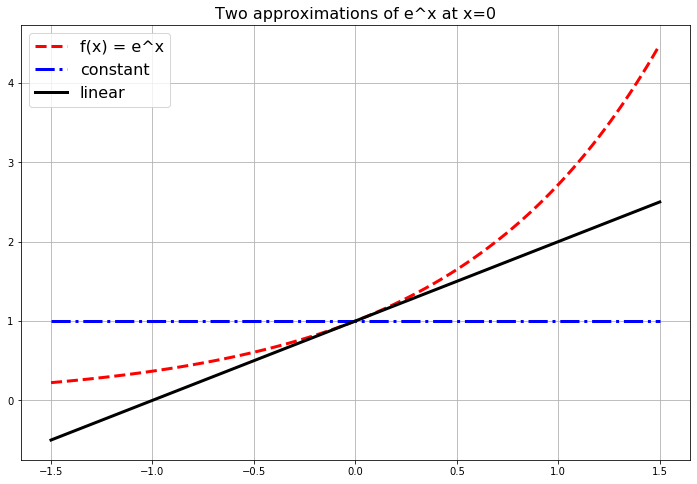
\includegraphics[width=0.75\linewidth]{images/Ch01Sec04_Taylor_exp1} 

}

\caption{The first few Taylor approximations of the exponential function.}\label{fig:taylor-exp1}
\end{figure}

\begin{center}\rule{0.5\linewidth}{0.5pt}\end{center}

\begin{exercise}
\protect\hypertarget{exr:unnamed-chunk-33}{}{\label{exr:unnamed-chunk-33} }Let's extend the idea from the previous problem to much better approximations of the function \(f(x) = e^x\).

\begin{enumerate}
\def\labelenumi{\alph{enumi}.}
\tightlist
\item
  Let's build a function \(g(x)\) that matches \(f(x)\) exactly at \(x=0\), has exactly the same first derivative as \(f(x)\) at \(x=0\), AND has exactly the same second derivative as \(f(x)\) at \(x=0\). To do this we'll use a quadratic function. For a quadratic approximation of a function we just take a slight extension to the point-slope form of a line and use the equation
  \[ y = f(x_0) + f'(x_0) (x-x_0) + \frac{f''(x_0)}{2} (x-x_0)^2. \]
  In this case we are using \(x_0 = 0\) so the quadratic approximation function looks like
  \[ y = f(0) + f'(0) x + \frac{f''(0)}{2} x^2. \]

  \begin{enumerate}
  \def\labelenumii{\roman{enumii}.}
  \tightlist
  \item
    Find the quadratic approximation for \(f(x) = e^x\).
  \item
    How do you know that this function matches \(f(x)\) is all of the ways described above at \(x=0\)?
  \item
    Add your new function to the plot you created in the previous problem.\\
  \end{enumerate}
\item
  Let's keep going!! Next we'll do a cubic approximation. A cubic approximation takes the form
  \[ y = f(x_0) + f'(0) (x-x_0) + \frac{f''(0)}{2}(x-x_0)^2 + \frac{f'''(0)}{3!}(x-x_0)^3 \]

  \begin{enumerate}
  \def\labelenumii{\roman{enumii}.}
  \tightlist
  \item
    Find the cubic approximation for \(f(x) = e^x\).
  \item
    How do we know that this function matches the first, second, and third derivatives of \(f(x)\) at \(x=0\)?
  \item
    Add your function function to the plot.
  \item
    Pause and think: What's the deal with the \(3!\) on the cubic term?\\
  \end{enumerate}
\item
  Your turn: Build the next several approximations of \(f(x) = e^x\) at \(x=0\). Add these plots to the plot that we've been building all along.
\end{enumerate}
\end{exercise}

\begin{center}\rule{0.5\linewidth}{0.5pt}\end{center}

\begin{exercise}
\protect\hypertarget{exr:unnamed-chunk-34}{}{\label{exr:unnamed-chunk-34} }We can get a decimal expansion of \(e\) pretty easily:
\[ e \approx 2.718281828459045 \]
In Python just type \texttt{np.exp(1)} which will just evaluate \(f(x) = e^x\) at \(x=1\) (and hence giving you a value for \(e^1 = e\)). We built our approximations in the previous problems centered at \(x=0\), and \(x=1\) is \emph{not too terribly} far from \(x=0\) so perhaps we can get a good approximation with the functions that we've already built. Complete the following table to see how we did with our approximations.

\begin{longtable}[]{@{}lll@{}}
\toprule
Approximation Function & Value at \(x=1\) & Absolute Error\tabularnewline
\midrule
\endhead
Constant & 1 & \(| 2.71828... - 1| \approx 1.71828...\)\tabularnewline
Linear & 1+1=2 & \(|2.71828... - 2| \approx 0.71828...\)\tabularnewline
Quadratic & &\tabularnewline
Cubic & &\tabularnewline
Quartic & &\tabularnewline
Quintic & &\tabularnewline
\bottomrule
\end{longtable}
\end{exercise}

\begin{center}\rule{0.5\linewidth}{0.5pt}\end{center}

\begin{exercise}
\protect\hypertarget{exr:unnamed-chunk-35}{}{\label{exr:unnamed-chunk-35} }Use the functions that you've built to approximate \(\sqrt{e} = e^{0.5}\). Check the accuracy of your answer using \texttt{np.exp(0.5)} in Python.
\end{exercise}

\begin{center}\rule{0.5\linewidth}{0.5pt}\end{center}

\begin{exercise}
\protect\hypertarget{exr:unnamed-chunk-36}{}{\label{exr:unnamed-chunk-36} }Use the functions that you've built to approximate \(\frac{1}{e} = e^{-1}\). Check the accuracy of your answer using \texttt{np.exp(-1)} in Python.
\end{exercise}

\begin{center}\rule{0.5\linewidth}{0.5pt}\end{center}

What we've been exploring so far in this section is the \textbf{Taylor Series} of a function.

\begin{definition}[Taylor Series]
\protect\hypertarget{def:unnamed-chunk-37}{}{\label{def:unnamed-chunk-37} \iffalse (Taylor Series) \fi{} }If \(f(x)\) is an infinitely differentiable function at the point \(x_0\) then
\[ f(x) = f(x_0) + f'(x_0)(x-x_0) + \frac{f''(x_0)}{2}(x-x_0)^2 + \cdots \frac{f^{(n)}(x_0)}{n!}(x-x_0)^n + \cdots  \]
for any reasonably small interval around \(x_0\). The infinite polynomial expansion is called the \textbf{Taylor Series} of the function \(f(x)\). Taylor Series are named for the mathematician \href{https://en.wikipedia.org/wiki/Brook_Taylor}{Brook Taylor}.
\end{definition}

\begin{center}\rule{0.5\linewidth}{0.5pt}\end{center}

The Taylor Series of a function is often written with summation notation as
\[ f(x) = \sum_{k=0}^\infty \frac{f^{(k)}(x_0)}{k!} (x-x_0)^k. \]
Don't let the notation scare you. In a Taylor Series you are just saying: \emph{give me a function that}

\begin{itemize}
\tightlist
\item
  \emph{matches \(f(x)\) at \(x=x_0\) exactly,}
\item
  \emph{matches \(f'(x)\) at \(x=x_0\) exactly,}
\item
  \emph{matches \(f''(x)\) at \(x=x_0\) exactly,}
\item
  \emph{matches \(f'''(x)\) at \(x=x_0\) exactly,}
\item
  etc.
\end{itemize}

(Take a moment and make sure that the summation notation makes sense to you.)

Moreover, Taylor Series are built out of the easiest types of functions: polynomials. Computers are rather good at doing computations with addition, subtraction, multiplication, division, and integer exponents, so Taylor Series are a natural way to express functions in a computer. The down side is that we can only get true equality in the Taylor Series if we have infinitely many terms in the series. A computer cannot do infinitely many computations. So, in practice, we truncate Taylor Series after many terms and think of the new polynomial function as being \emph{close enough} to the actual function so far as we don't stray too far from the anchor \(x_0\).

\begin{center}\rule{0.5\linewidth}{0.5pt}\end{center}

\begin{definition}[Maclaurin Series]
\protect\hypertarget{def:unnamed-chunk-38}{}{\label{def:unnamed-chunk-38} \iffalse (Maclaurin Series) \fi{} }A Taylor Series that is centered at \(x_0 = 0\) is called a Maclaurin Series after the mathematician \href{https://en.wikipedia.org/wiki/Colin_Maclaurin}{Colin Maclaurin}. This is just a special case of a Taylor Series, so throughout this book we will refer to both Taylor Series and Maclaurin Series simply as Taylor Series.
\end{definition}

\begin{center}\rule{0.5\linewidth}{0.5pt}\end{center}

\begin{exercise}
\protect\hypertarget{exr:unnamed-chunk-39}{}{\label{exr:unnamed-chunk-39} }Verify from your previous work that the Taylor Series centered at \(x_0 = 0\) (i.e.~the Maclaurin Series) for \(f(x) = e^x\) is indeed
\[ e^x = 1 + x + \frac{x^2}{2} + \frac{x^3}{3!} + \frac{x^4}{4!} + \frac{x^5}{5!} + \cdots. \]
\end{exercise}

\begin{center}\rule{0.5\linewidth}{0.5pt}\end{center}

\begin{exercise}
\protect\hypertarget{exr:unnamed-chunk-40}{}{\label{exr:unnamed-chunk-40} }Do all of the calculations to show that the Taylor Series centered at \(x_0 = 0\) for the function \(f(x) = \sin(x)\) is indeed
\[ \sin(x) = x - \frac{x^3}{3!} + \frac{x^5}{5!} - \frac{x^7}{7!} + \cdots \]
\end{exercise}

\begin{center}\rule{0.5\linewidth}{0.5pt}\end{center}

\begin{exercise}
\protect\hypertarget{exr:unnamed-chunk-41}{}{\label{exr:unnamed-chunk-41} }Do all of the calculations to show that the Taylor Series centered at \(x_0 = 0\) for the function \(f(x) = \cos(x)\) is indeed
\[ \cos(x) = 1 - \frac{x^2}{2!} + \frac{x^4}{4!} - \frac{x^6}{6!} + \cdots \]
\end{exercise}

\begin{center}\rule{0.5\linewidth}{0.5pt}\end{center}

\begin{exercise}
\protect\hypertarget{exr:unnamed-chunk-42}{}{\label{exr:unnamed-chunk-42} }Let's compute a few Taylor Series that are not centered at \(x_0 = 0\) (that is, Taylor Series that are not Maclaurin Series). For example, let's approximate the function \(f(x) = \sin(x)\) near \(x_0 = \frac{\pi}{2}\). Near the point \(x_0 = \frac{\pi}{2}\), the Taylor Series approximation will take the form
\[ f(x) = f\left( \frac{\pi}{2} \right) + f'\left( \frac{\pi}{2} \right)\left( x - \frac{\pi}{2} \right) + \frac{f''\left( \frac{\pi}{2} \right)}{2!}\left( x - \frac{\pi}{2} \right)^2 + \frac{f'''\left( \frac{\pi}{2} \right)}{3!}\left( x - \frac{\pi}{2} \right)^3 + \cdots \]

Write the first several terms of the Taylor Series for \(f(x) = \sin(x)\) centered at \(x_0 = \frac{\pi}{2}\). Then write Python code to build the plot below showing successive approximations for \(f(x) = \sin(x)\) centered at \(\pi/2\).
\end{exercise}

\begin{figure}

{\centering 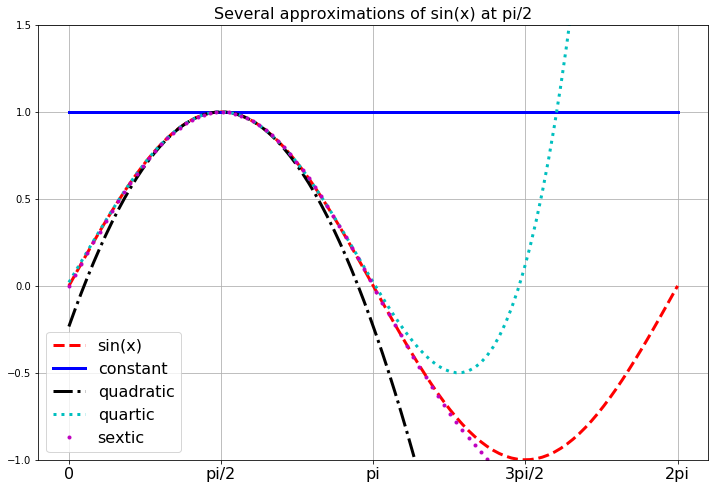
\includegraphics[width=0.75\linewidth]{images/Ch01Sec04_Taylor_Sine_pi2} 

}

\caption{Taylor Series approximations of $f(x) = sin(x)$.}\label{fig:taylor-sine-pi2}
\end{figure}

\begin{center}\rule{0.5\linewidth}{0.5pt}\end{center}

\begin{exercise}
\protect\hypertarget{exr:unnamed-chunk-43}{}{\label{exr:unnamed-chunk-43} }Repeat the previous exercise for the functions
\begin{eqnarray}
  f(x) &= \cos(x) \text{ centered at } x_0 = \pi \\
  f(x) &= \ln(x) \text{ centered at } x_0 = 1
\end{eqnarray}
\end{exercise}

\begin{center}\rule{0.5\linewidth}{0.5pt}\end{center}

\begin{exercise}
\protect\hypertarget{exr:unnamed-chunk-44}{}{\label{exr:unnamed-chunk-44} }Approximate \(\cos(3)\) using a Taylor Series.
\end{exercise}

\begin{center}\rule{0.5\linewidth}{0.5pt}\end{center}

\begin{exercise}
\protect\hypertarget{exr:unnamed-chunk-45}{}{\label{exr:unnamed-chunk-45} }Approximate \(\ln(1.1)\) using a Taylor Series.
\end{exercise}

\begin{center}\rule{0.5\linewidth}{0.5pt}\end{center}

\begin{example}
\protect\hypertarget{exm:unnamed-chunk-46}{}{\label{exm:unnamed-chunk-46} }Let's conclude this brief section by examining an interesting example. Consider the function
\[ f(x) = \frac{1}{1-x}. \]
If we build a Taylor Series centered at \(x_0 = 0\) (i.e.~the Maclaurin Series) it isn't too hard to show that we get
\[ f(x) = 1 + x + x^2 + x^3 + x^4 + x^5 + \cdots \]
(you should stop now and verify this!). However, if we plot the function \(f(x)\) along with several successive approximations for \(f(x)\) we find that beyond \(x=1\) we don't get the correct behavior of the function (see Figure \ref{fig:taylor-3}). More specifically, we cannot get the Taylor Series to change behavior across the vertical asymptote of the function at \(x=1\). This example is meant to point out the fact that a Taylor Series will only ever make sense \emph{near} the point at which you center the expansion. For the function \(f(x) = \frac{1}{1-x}\) centered at \(x_0 = 0\) we can only get good approximations within the interval \(x \in (-1,1)\) and no further.
\end{example}

\begin{figure}

{\centering 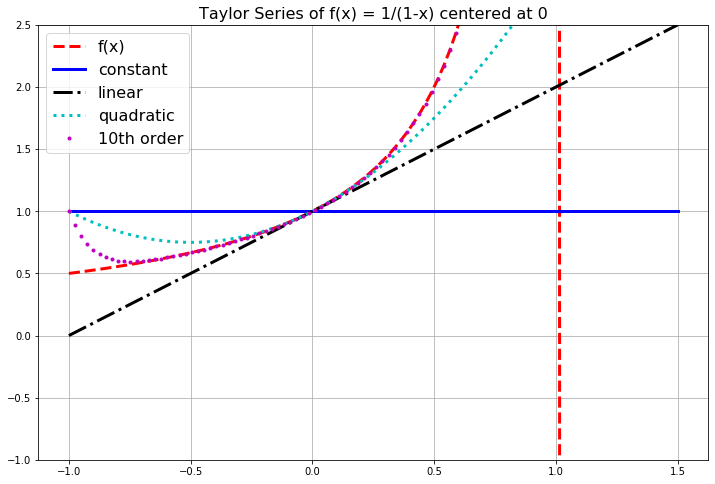
\includegraphics[width=0.75\linewidth]{images/Ch01Sec04_Taylor3} 

}

\caption{Several Taylor Series approximations of the function $f(x) = 1/(1-x)$.}\label{fig:taylor-3}
\end{figure}

\begin{center}\rule{0.5\linewidth}{0.5pt}\end{center}

In the previous example we saw that we cannot always get approximations from Taylor Series that are good everywhere. For every Taylor Series there is a \textbf{domain of convergence} where the Taylor Series actually makes sense and gives good approximations. While it is beyond the scope of this section to give all of the details for finding the domain of convergence for a Taylor Series, a good heuristic is to observe that a Taylor Series will only give reasonable approximations of a function from the center of the series to the nearest asymptote. The domain of convergence is typically symmetric about the center as well. For example:

\begin{itemize}
\tightlist
\item
  If we were to build a Taylor Series approximation for the function \(f(x) = \ln(x)\) centered at the point \(x_0 = 1\) then the radius of convergence should be \(x \in (0,2)\) since there is a vertical asymptote for the natural logarithm function at \(x=0\).
\item
  If we were to build a Taylor Series approximation for the function \(f(x) = \frac{5}{2x-3}\) centered at the point \(x_0 = 4\) then the radius of convergence should be \(x \in (1.5, 6.5)\) since there is a vertical asymptote at \(x=1.5\) and the distance from \(x_0 = 4\) to \(x=1.5\) is 2.5 units.\\
\item
  If we were to build a Taylor Series approximation for the function \(f(x) = \frac{1}{1+x^2}\) centered at the point \(x_0 = 0\) then the radius of convergence should be \(x \in (-1,1)\). This may seem quite odd (and perhaps quite surprising!) but let's think about where the nearest asymptote might be. To find the asymptote we need to solve \(1+x^2 = 0\) but this gives us the values \(x = \pm i\). In the complex plane, the numbers \(i\) and \(-i\) are 1 unit away from \(x_0 = 0\), so the ``asymptote'' isn't visible in a real-valued plot but it is still only one unit away. Hence the domain of convergence is \(x \in (-1,1)\). You should pause now and build some plots to show yourself that this indeed appears to be true.\footnote{The cover photo of the book shows the first several terms of the Taylor Series for this function. The convergence in the interval \(x \in (-1,1)\) is pretty clear from the picture.}
\end{itemize}

A Taylor Series will give good approximations to the function within the domain of convergence, but will give garbage outside of it. For more details about the domain of convergence of a Taylor Series you can refer to the \href{https://activecalculus.org/single/sec-8-5-taylor.html}{Taylor Series section of the online Active Calculus Textbook} {[}\protect\hyperlink{ref-active-calculus}{2}{]}.

\hypertarget{approximation-error-with-taylor-series}{%
\section{Approximation Error with Taylor Series}\label{approximation-error-with-taylor-series}}

The great thing about Taylor Series is that they allow for the
representation of potentially very complicated functions as polynomials -- and polynomials are
easily dealt with on a computer since they involve only addition,
subtraction, multiplication, division, and integer powers. The down side is that
the order of the polynomial is infinite. Hence, every time we use a Taylor series on a
computer we are actually going to be using a \textbf{Truncated Taylor Series}
where we only take a finite number of terms. The idea here is simple in principle:

\begin{itemize}
\tightlist
\item
  If a function \(f(x)\) has a Taylor Series representation it can be written as an infinite sum.
\item
  Computers can't do infinite sums.
\item
  So stop the sum at some point \(n\) and throw away the rest of the infinite sum.
\item
  Now \(f(x)\) is approximated by some finite sum so long as you stay pretty close to \(x = x_0\),
\item
  and everything that we just chopped off of the end is called the \textbf{remainder} for the finite sum.
\end{itemize}

Let's be a bit more concrete about it. The Taylor Series for \(f(x) = e^x\) centered at \(x_0 = 0\) is
\[ e^x = 1 + x + \frac{x^2}{2!} + \frac{x^3}{3!} + \frac{x^4}{4!} + \cdots. \]

\begin{description}
\item[\(0^{th}\) Order Approximation of \(f(x) = e^x\):]
If we want to use a zeroth-order (constant) approximation of \(f(x) = e^x\) then we only take the first term in the Taylor Series and the rest is not used for the approximation
\[ e^x = \underbrace{1}_{\text{$0^{th}$ order approximation}} + \underbrace{x + \frac{x^2}{2!} + \frac{x^3}{3!} + \frac{x^4}{4!} + \cdots}_{\text{remainder}}. \]
Therefore we would approximate \(e^x\) as \(e^x \approx 1\) for values of \(x\) that are close to \(x_0 = 0\). Furthermore, for small values of \(x\) that are close to \(x_0 = 0\) the largest term in the remainder is \(x\) (since for small values of \(x\) like 0.01, \(x^2\) will be even smaller, \(x^3\) even smaller than that, etc). This means that if we use a \(0^{th}\) order approximation for \(e^x\) then we expect our error to be about the same size as \(x\). It is common to then rewrite the truncated Taylor Series as
\[ \text{$0^{th}$ order approximation: } e^x \approx 1 + \mathcal{O}(x) \]
where \(\mathcal{O}(x)\) (read ``Big-O of \(x\)'') tells us that the expected error for approximations close to \(x_0 = 0\) is about the same size as \(x\).
\item[\(1^{st}\) Order Approximation of \(f(x) = e^x\):]
If we want to use a first-order (linear) approximation of \(f(x) = e^x\) then we gather the \(0^{th}\) order and \(1^{st}\) order terms together as our approximation and the rest is the remainder
\[ e^x = \underbrace{1 + x}_{\text{$1^{st}$ order approximation}} + \underbrace{\frac{x^2}{2!} + \frac{x^3}{3!} + \frac{x^4}{4!} + \cdots}_{\text{remainder}}. \]
Therefore we would approximate \(e^x\) as \(e^x \approx 1+x\) for values of \(x\) that are close to \(x_0 = 0\). Furthermore, for values of \(x\) very close to \(x_0 = 0\) the largest term in the remainder is the \(x^2\) term. Using Big-O notation we can write the approximation as
\[ \text{$1^{st}$ order approximation: } e^x \approx 1 + x + \mathcal{O}(x^2). \]
Notice that we don't explicitly say what the coefficient is for the \(x^2\) term. Instead we are just saying that \emph{using the linear function \(y=1+x\) to approximate \(e^x\) for values of \(x\) near \(x_0=0\) will result in errors that are proportional to \(x^2\).}
\item[\(2^{nd}\) Order Approximation of \(f(x) = e^x\):]
If we want to use a second-order (quadratic) approximation of \(f(x) = e^x\) then we gather the \(0^{th}\) order, \(1^{st}\) order, and \(2^{nd}\) order terms together as our approximation and the rest is the remainder
\[ e^x = \underbrace{1 + x + \frac{x^2}{2!}}_{\text{$2^{nd}$ order approximation}} + \underbrace{\frac{x^3}{3!} + \frac{x^4}{4!} + \cdots}_{\text{remainder}}. \]
Therefore we would approximate \(e^x\) as \(e^x \approx 1+x+\frac{x^2}{2}\) for values of \(x\) that are close to \(x_0 = 0\). Furthermore, for values of \(x\) very close to \(x_0 = 0\) the largest term in the remainder is the \(x^3\) term. Using Big-O notation we can write the approximation as
\[ \text{$2^{nd}$ order approximation: } e^x \approx 1 + x + \frac{x^2}{2} + \mathcal{O}(x^3). \]
Again notice that we don't explicitly say what the coefficient is for the \(x^3\) term. Instead we are just saying that \emph{using the quadratic function \(y=1+x+\frac{x^2}{2}\) to approximate \(e^x\) for values of \(x\) near \(x_0=0\) will result in errors that are proportional to \(x^3\).}
\end{description}

For the function \(f(x) = e^x\) the idea of approximating the amount of approximation error by truncating the Taylor Series is relatively straight forward: if we want an \(n^{th}\) order polynomial approximation of \(e^x\) near \(x_0 = 0\) then
\[ e^x = 1 + x + \frac{x^2}{2!} + \frac{x^3}{3!} + \frac{x^4}{4!} + \cdots + \frac{x^n}{n!} + \mathcal{O}(x^{n+1}) \]
meaning that we expect the error to be proportional to \(x^{n+1}\).

Keep in mind that this sort of analysis is only good for values of \(x\) that are very close to the center of the Taylor Series. If you are making approximations that are too far away then all bets are off.

\begin{center}\rule{0.5\linewidth}{0.5pt}\end{center}

\begin{exercise}
\protect\hypertarget{exr:unnamed-chunk-47}{}{\label{exr:unnamed-chunk-47} }Let's make the previous discussion a bit more concrete. We know the Taylor Series for \(f(x) = e^x\) quite well at this point so let's use it to approximate the value of \(f(0.1) = e^{0.1}\) with different order polynomials. Notice that \(x=0.1\) is pretty close to the center of the Taylor Series \(x_0 = 0\) so this sort of approximation is reasonable.

Using \texttt{np.exp(0.1)} we have Python's approximation \(e^{0.1} \approx\) \texttt{np.exp(0.1)} \(=1.1051709181\).

Fill in the blanks in the table.

\begin{longtable}[]{@{}llll@{}}
\toprule
\begin{minipage}[b]{0.23\columnwidth}\raggedright
Taylor Series\strut
\end{minipage} & \begin{minipage}[b]{0.23\columnwidth}\raggedright
Approximation\strut
\end{minipage} & \begin{minipage}[b]{0.23\columnwidth}\raggedright
Absolute Error\strut
\end{minipage} & \begin{minipage}[b]{0.19\columnwidth}\raggedright
Expected Error\strut
\end{minipage}\tabularnewline
\midrule
\endhead
\begin{minipage}[t]{0.23\columnwidth}\raggedright
\(0^{th}\) Order\strut
\end{minipage} & \begin{minipage}[t]{0.23\columnwidth}\raggedright
\(1\)\strut
\end{minipage} & \begin{minipage}[t]{0.23\columnwidth}\raggedright
\(|e^{0.1}-1| = 0.1051709181\)\strut
\end{minipage} & \begin{minipage}[t]{0.19\columnwidth}\raggedright
\(\mathcal{O}(x) = 0.1\)\strut
\end{minipage}\tabularnewline
\begin{minipage}[t]{0.23\columnwidth}\raggedright
\(1^{st}\) Order\strut
\end{minipage} & \begin{minipage}[t]{0.23\columnwidth}\raggedright
\(1.1\)\strut
\end{minipage} & \begin{minipage}[t]{0.23\columnwidth}\raggedright
\(|e^{0.1}-1.1| = 0.0051709181\)\strut
\end{minipage} & \begin{minipage}[t]{0.19\columnwidth}\raggedright
\(\mathcal{O}(x^2) = 0.1^2 = 0.01\)\strut
\end{minipage}\tabularnewline
\begin{minipage}[t]{0.23\columnwidth}\raggedright
\(2^{nd}\) Order\strut
\end{minipage} & \begin{minipage}[t]{0.23\columnwidth}\raggedright
\(1.105\)\strut
\end{minipage} & \begin{minipage}[t]{0.23\columnwidth}\raggedright
\strut
\end{minipage} & \begin{minipage}[t]{0.19\columnwidth}\raggedright
\strut
\end{minipage}\tabularnewline
\begin{minipage}[t]{0.23\columnwidth}\raggedright
\(3^{rd}\) Order\strut
\end{minipage} & \begin{minipage}[t]{0.23\columnwidth}\raggedright
\strut
\end{minipage} & \begin{minipage}[t]{0.23\columnwidth}\raggedright
\strut
\end{minipage} & \begin{minipage}[t]{0.19\columnwidth}\raggedright
\strut
\end{minipage}\tabularnewline
\begin{minipage}[t]{0.23\columnwidth}\raggedright
\(4^{th}\) Order\strut
\end{minipage} & \begin{minipage}[t]{0.23\columnwidth}\raggedright
\strut
\end{minipage} & \begin{minipage}[t]{0.23\columnwidth}\raggedright
\strut
\end{minipage} & \begin{minipage}[t]{0.19\columnwidth}\raggedright
\strut
\end{minipage}\tabularnewline
\begin{minipage}[t]{0.23\columnwidth}\raggedright
\(5^{th}\) Order\strut
\end{minipage} & \begin{minipage}[t]{0.23\columnwidth}\raggedright
\strut
\end{minipage} & \begin{minipage}[t]{0.23\columnwidth}\raggedright
\strut
\end{minipage} & \begin{minipage}[t]{0.19\columnwidth}\raggedright
\strut
\end{minipage}\tabularnewline
\bottomrule
\end{longtable}
\end{exercise}

\begin{center}\rule{0.5\linewidth}{0.5pt}\end{center}

Observe in the previous exercise that the actual absolute error and the expected error get closer and closer to each other. Using the first term in the remainder to estimate the approximation error of truncating a Taylor Series is crude but very easy to implement.

\begin{center}\rule{0.5\linewidth}{0.5pt}\end{center}

\begin{theorem}
\protect\hypertarget{thm:unnamed-chunk-48}{}{\label{thm:unnamed-chunk-48} }The approximation error when using a truncated Taylor Series is roughly proportional to the size of the next term in the Taylor Series.
\end{theorem}

\begin{center}\rule{0.5\linewidth}{0.5pt}\end{center}

\begin{exercise}
\protect\hypertarget{exr:unnamed-chunk-49}{}{\label{exr:unnamed-chunk-49} }Next we will examine the approximation error for the sine function near \(x_0 = 0\). We know that the sine function has the Taylor Series centered at \(x_0 = 0\) as
\[ \sin(x) = x - \frac{x^3}{3!} + \frac{x^5}{5!} - \frac{x^7}{7!} + \cdots. \]

\begin{enumerate}
\def\labelenumi{\alph{enumi}.}
\tightlist
\item
  A linear approximation of \(\sin(x)\) near \(x_0 = 0\) is \(\sin(x) = x + \mathcal{O}(x^3)\).

  \begin{enumerate}
  \def\labelenumii{\roman{enumii}.}
  \tightlist
  \item
    Use the linear approximation formula to approximate \(\sin(0.2)\).
  \item
    What does ``\(\mathcal{O}(x^3)\)'' mean about the approximation of \(\sin(0.2)\)?\\
    (Take note that we ignore the minus sign on the approximation error since we are really only interested in absolute error (i.e.~we don't care if we overshoot or undershoot).)
  \end{enumerate}
\item
  Notice that there are no quadratic terms in the Taylor Series so there is no quadratic approximation for \(\sin(x)\) near \(x_0 =0\).
\item
  A cubic approximation of \(\sin(x)\) near \(x_0 = 0\) is \(\sin(x) = ?? - ?? + \mathcal{O}(??)\).

  \begin{enumerate}
  \def\labelenumii{\roman{enumii}.}
  \tightlist
  \item
    Fill in the question marks in the cubic approximation formula.
  \item
    Use the linear approximation formula to approximate \(\sin(0.2)\).
  \item
    What is the approximation error for your approximation?
  \end{enumerate}
\item
  What is the next approximation formula for \(\sin(x)\) near \(x_0 = 0\)? Use it to approximate \(\sin(0.2)\), and give the expected approximation error.
\item
  Now let's check all of our answers against what Python says we should get for \(\sin(0.2)\). If you use \texttt{np.sin(0.2)} you should get \(\sin(0.2) \approx\) \texttt{np.sin(0.2)} \(=0.1986693308\). Fill in the blanks in the table below and then discuss the quality of our error approximations.
\end{enumerate}

\begin{longtable}[]{@{}lll@{}}
\toprule
Taylor Series & Estimated Error & Actual Absolute Error\tabularnewline
\midrule
\endhead
\(1^{st}\) Order & \(\mathcal{O}(x^3) = 0.2^3 = 0.008\) & \(0.001330669205\)\tabularnewline
\(3^{rd}\) Order & &\tabularnewline
\(5^{th}\) Order & &\tabularnewline
\(7^{th}\) Order & &\tabularnewline
\(9^{th}\) Order & &\tabularnewline
\bottomrule
\end{longtable}

\begin{enumerate}
\def\labelenumi{\alph{enumi}.}
\setcounter{enumi}{5}
\tightlist
\item
  What observations do you make about the estimate of the approximation error and the actual approximation error?\\
\end{enumerate}
\end{exercise}

\begin{center}\rule{0.5\linewidth}{0.5pt}\end{center}

\begin{exercise}
\protect\hypertarget{exr:unnamed-chunk-50}{}{\label{exr:unnamed-chunk-50} }What if we want an approximation of \(\ln(1.1)\) and we want that approximation to be within 5 decimal places. The number 1.1 is very close to 1 and we know that \(\ln(1) = 0\). Hence, it seems like a good idea to build a Taylor Series approximation for \(\ln(x)\) centered at \(x_0 = 1\) to solve this problem.

\begin{enumerate}
\def\labelenumi{\alph{enumi}.}
\tightlist
\item
  Complete the table of derivatives below to get the Taylor coefficients for the Taylor Series of \(\ln(x)\) centered at \(x_0 = 1\).
\end{enumerate}

\begin{longtable}[]{@{}llll@{}}
\toprule
Order of Derivative & Derivative & Value at \(x_0 = 1\) & Taylor Coefficient\tabularnewline
\midrule
\endhead
0 & \(\ln(x)\) & 0 & 0\tabularnewline
1 & \(\frac{1}{x} = x^{-1}\) & 1 & 1\tabularnewline
2 & \(-x^{-2}\) & \(-1\) & \(\frac{-1}{2!} = -\frac{1}{2}\)\tabularnewline
3 & \(2x^{-3}\) & 2 & \(\frac{2}{3!} = \frac{1}{3}\)\tabularnewline
4 & \(-6x^{-4}\) & \(-6\) &\tabularnewline
5 & & &\tabularnewline
6 & & &\tabularnewline
\(\vdots\) & \(\vdots\) & \(\vdots\) & \(\vdots\)\tabularnewline
\bottomrule
\end{longtable}

\begin{enumerate}
\def\labelenumi{\alph{enumi}.}
\setcounter{enumi}{1}
\tightlist
\item
  Based on what you did in part (a), complete the Taylor Series for \(\ln(x)\) centered at \(x_0 = 1\).
  \[ \ln(x) = 0 + 1(x-1) - \frac{1}{2}(x-1)^2 + \frac{1}{3}(x-1)^3 - \frac{??}{??}(x-1)^4 + \frac{??}{??}(x-1)^5 + \cdots. \]
\item
  The \(n^{th}\) order Taylor approximation of \(\ln(x)\) near \(x_0 = 1\) is given below. What is the order of the estimated approximation error?
  \[ \ln(x) = (x-1) - \frac{(x-1)^2}{2} + \frac{(x-1)^3}{3} - \cdots + \frac{(-1)^{n-1} (x-1)^n}{n} + \mathcal{O}(???) \]
\item
  Finally we want to get an approximation for \(\ln(1.1)\) accurate to 5 decimal places (or better). What is the minimum number of terms we expect to need from the Taylor Series? Support your answer mathematically.
\item
  Use Python's \texttt{np.log(1.1)} to get an approximation for \(\ln(1.1)\) and then numerically verify your answer to part (d).
\end{enumerate}
\end{exercise}

\begin{center}\rule{0.5\linewidth}{0.5pt}\end{center}

\begin{exercise}
\protect\hypertarget{exr:unnamed-chunk-51}{}{\label{exr:unnamed-chunk-51} }In the previous problem you found an approximation for \(\ln(1.1)\) to 5 decimal places. In doing so you had to build a Taylor Series at a well-known point nearby 1.1 and then use our approximation of the error to determine the number of terms to keep in the approximation. In this exercise we want an approximation of \(\cos\left( \frac{\pi}{2} + 0.05 \right)\). To do so you should build a Taylor Series for the cosine function centered at an appropriate point, determine an estimate for the approximation error, and then use that estimate to determine the number of terms to keep in the approximation.
\end{exercise}

\begin{center}\rule{0.5\linewidth}{0.5pt}\end{center}

\hypertarget{exercises}{%
\section{Exercises}\label{exercises}}

\hypertarget{coding-exercises}{%
\subsection{Coding Exercises}\label{coding-exercises}}

The first several exercises here are meant for you to practice and
improve your coding skills. If you are stuck on any of the coding then I recommend that you have a look at Appendix \ref{ch:python}. Please refrain from Googling anything on these problems. The point is to struggle through the code, get it wrong many times, debug, and then to eventually have working code.

\begin{center}\rule{0.5\linewidth}{0.5pt}\end{center}

\begin{exercise}
\protect\hypertarget{exr:unnamed-chunk-52}{}{\label{exr:unnamed-chunk-52} }(This problem is modified from {[}\protect\hyperlink{ref-euler}{3}{]})\\
If we list all of the numbers below 10 that are multiples of 3 or 5 we
get 3, 5, 6, and 9. The sum of these multiples is 23. Write code to find
the sum of all the multiples of 3 or 5 below 1000. Your code needs to
run error free and output only the sum.
\end{exercise}

\begin{center}\rule{0.5\linewidth}{0.5pt}\end{center}

\begin{exercise}
\protect\hypertarget{exr:unnamed-chunk-53}{}{\label{exr:unnamed-chunk-53} }(This problem is modified from {[}\protect\hyperlink{ref-euler}{3}{]})\\
Each new term in the Fibonacci sequence is generated by adding the
previous two terms. By starting with 1 and 2, the first 10 terms will
be: \[1, 2, 3, 5, 8, 13, 21, 34, 55, 89, \dots\] By considering the
terms in the Fibonacci sequence whose values do not exceed four million,
write code to find the sum of the even-valued terms. Your code needs to
run error free and output only the sum.
\end{exercise}

\begin{center}\rule{0.5\linewidth}{0.5pt}\end{center}

\begin{exercise}
\protect\hypertarget{exr:unnamed-chunk-54}{}{\label{exr:unnamed-chunk-54} }Write computer code that will draw random numbers from the unit interval
\([0,1]\), distributed uniformly (using Python's \texttt{np.random.rand()}), until the sum of the numbers that you
draw is greater than 1. Keep track of how many numbers you draw. Then
write a loop that does this process many many times. On average, how
many numbers do you have to draw until your sum is larger than 1?

\begin{description}
\item[Hint \#1:]
Use the \texttt{np.random.rand()}command to
draw a single number from a uniform distribution with bounds \((0,1)\).\\
\item[Hint \#2:]
You should do this more than 1,000,000 times to get a good
average \ldots and the number that you get should be familiar!
\end{description}
\end{exercise}

\begin{center}\rule{0.5\linewidth}{0.5pt}\end{center}

\begin{exercise}
\protect\hypertarget{exr:unnamed-chunk-55}{}{\label{exr:unnamed-chunk-55} }My favorite prime number is 8675309. Yep. Jenny's phone number is prime!
Write a script that verifies this fact.

\begin{description}
\item[Hint:]
You only need to check divisors as large as the square root of 8675309 (why).
\end{description}
\end{exercise}

\begin{center}\rule{0.5\linewidth}{0.5pt}\end{center}

\begin{exercise}
\protect\hypertarget{exr:unnamed-chunk-56}{}{\label{exr:unnamed-chunk-56} }(This problem is modified from {[}\protect\hyperlink{ref-euler}{3}{]})\\
Write a function called that accepts an integer and returns a binary
variable:
* 0 = not prime,
* 1 = prime.

Next write a script to find the sum of all of the prime numbers less than 1000.

\begin{description}
\item[Hint:]
Remember that a prime number has exactly two divisors: 1 and itself. You only need to check divisors as large as the square root of \(n\). Your script should probably be smart enough to avoid all of the non-prime even numbers.
\end{description}
\end{exercise}

\begin{center}\rule{0.5\linewidth}{0.5pt}\end{center}

\begin{exercise}
\protect\hypertarget{exr:unnamed-chunk-57}{}{\label{exr:unnamed-chunk-57} }(This problem is modified from {[}\protect\hyperlink{ref-euler}{3}{]})\\
The sum of the squares of the first ten natural numbers is,
\[1^2 + 2^2 + \dots + 10^2 = 385\] The square of the sum of the first
ten natural numbers is, \[(1 + 2 + \dots + 10)^2 = 55^2 = 3025\] Hence
the difference between the sum of the squares of the first ten natural
numbers and the square of the sum is \(3025 - 385 = 2640\).
\end{exercise}

\begin{center}\rule{0.5\linewidth}{0.5pt}\end{center}

\begin{exercise}
\protect\hypertarget{exr:unnamed-chunk-58}{}{\label{exr:unnamed-chunk-58} }(This problem is modified from {[}\protect\hyperlink{ref-euler}{3}{]})\\
Write code to find the difference between the sum of the squares of the
first one hundred natural numbers and the square of the sum. Your code
needs to run error free and output only the difference.
\end{exercise}

\begin{center}\rule{0.5\linewidth}{0.5pt}\end{center}

\begin{exercise}
\protect\hypertarget{exr:unnamed-chunk-59}{}{\label{exr:unnamed-chunk-59} }(This problem is modified from {[}\protect\hyperlink{ref-euler}{3}{]})\\
The prime factors of \(13195\) are \(5, 7, 13\) and \(29\). Write code to find
the largest prime factor of the number \(600851475143\)? Your code needs
to run error free and output only the largest prime factor.
\end{exercise}

\begin{center}\rule{0.5\linewidth}{0.5pt}\end{center}

\begin{exercise}
\protect\hypertarget{exr:unnamed-chunk-60}{}{\label{exr:unnamed-chunk-60} }(This problem is modified from {[}\protect\hyperlink{ref-euler}{3}{]})\\
The number 2520 is the smallest number that can be divided by each of
the numbers from 1 to 10 without any remainder. Write code to find the
smallest positive number that is evenly divisible by all of the numbers
from 1 to 20?

\textbf{Hint:} You will likely want to use \href{https://python-reference.readthedocs.io/en/latest/docs/operators/modulus.html}{modular division} for this problem.
\end{exercise}

\begin{center}\rule{0.5\linewidth}{0.5pt}\end{center}

\begin{exercise}
\protect\hypertarget{exr:unnamed-chunk-61}{}{\label{exr:unnamed-chunk-61} }The following iterative sequence is defined for the set of positive
integers:
\[\begin{aligned}
        & n \to \frac{n}{2} \quad \text{(n is even)} \\
        & n \to 3n + 1 \quad \text{(n is odd)}
    \end{aligned}\]
Using the rule above and starting with \(13\), we
generate the following sequence:
\[13 \to  40 \to 20 \to 10 \to 5 \to 16 \to 8 \to 4 \to 2 \to 1\] It can
be seen that this sequence (starting at 13 and finishing at 1) contains
10 terms. Although it has not been proved yet (Collatz Problem), it is
thought that all starting numbers finish at 1.

Write code to determine which starting number, under one million,
produces the longest chain. NOTE: Once the chain starts the terms are
allowed to go above one million.
\end{exercise}

\begin{center}\rule{0.5\linewidth}{0.5pt}\end{center}

\hypertarget{applying-what-youve-learned}{%
\subsection{Applying What You've Learned}\label{applying-what-youve-learned}}

\begin{exercise}
\protect\hypertarget{exr:unnamed-chunk-62}{}{\label{exr:unnamed-chunk-62} }(This problem is modified from {[}\protect\hyperlink{ref-chartier}{4}{]})\\
Sometimes floating point arithmetic does not work like we would expect (and hope) as compared to by-hand mathematics. In each of the following problems we have a mathematical problem that the computer gets wrong. Explain why the computer is getting these wrong.

\begin{enumerate}
\def\labelenumi{\alph{enumi}.}
\tightlist
\item
  Mathematically we know that \(\sqrt{5}^2\) should just give us 5 back. In Python type \texttt{np.sqrt(5)**2\ ==\ 5}. What do you get and why do you get it?
\item
  Mathematically we know that \(\left( \frac{1}{49} \right) \cdot 49\) should just be 1. In Python type \texttt{(1/49)*49\ ==\ 1}. What do you get and why do you get it?
\item
  Mathematically we know that \(e^{\ln(3)}\) should just give us 3 back. In Python type \texttt{np.exp(np.log(3))\ ==\ 3}. What do you get and why do you get it?
\item
  Create your own example of where Python gets something incorrect because of floating point arithmetic.
\end{enumerate}
\end{exercise}

\begin{center}\rule{0.5\linewidth}{0.5pt}\end{center}

\begin{exercise}
\protect\hypertarget{exr:unnamed-chunk-63}{}{\label{exr:unnamed-chunk-63} }(This problem is modified from {[}\protect\hyperlink{ref-chartier}{4}{]})\\
In the 1999 movie \emph{Office Space}, a character creates a program that
takes fractions of cents that are truncated in a bank's transactions and
deposits them to his own account. This is idea has been attempted in the
past and now banks look for this sort of thing. In this problem you will
build a simulation of the program to see how long it takes to become a
millionaire.

\textbf{Assumptions:}

\begin{itemize}
\tightlist
\item
  Assume that you have access to 50,000 bank accounts.
\item
  Assume that the account balances are uniformly distributed between \$100 and \$100,000.
\item
  Assume that the annual interest rate on the accounts is 5\% and the interest is compounded daily and added to the accounts, except that fractions of cents are truncated.
\item
  Assume that your \texttt{illegal} account initially has a \$0 balance.
\end{itemize}

\textbf{Your Tasks:}

\begin{enumerate}
\def\labelenumi{\alph{enumi}.}
\tightlist
\item
  Explain what the code below does.
\end{enumerate}
\end{exercise}

\begin{Shaded}
\begin{Highlighting}[]
\ImportTok{import}\NormalTok{ numpy }\ImportTok{as}\NormalTok{ np}
\NormalTok{accounts }\OperatorTok{=} \DecValTok{100} \OperatorTok{+}\NormalTok{ (}\DecValTok{100000}\OperatorTok{{-}}\DecValTok{100}\NormalTok{) }\OperatorTok{*}\NormalTok{ np.random.rand(}\DecValTok{50000}\NormalTok{,}\DecValTok{1}\NormalTok{)}\OperatorTok{;}
\NormalTok{accounts }\OperatorTok{=}\NormalTok{ np.floor(}\DecValTok{100}\OperatorTok{*}\NormalTok{accounts)}\OperatorTok{/}\DecValTok{100}\OperatorTok{;}
\end{Highlighting}
\end{Shaded}

\begin{enumerate}
\def\labelenumi{\alph{enumi}.}
\setcounter{enumi}{1}
\tightlist
\item
  By hand (no computer) write the mathematical steps necessary to
  increase the accounts by (5/365)\% per day, truncate the accounts to
  the nearest penny, and add the truncated amount into an account
  titled ``illegal''.
\item
  Write code to complete your plan from part (b).
\item
  Using a \texttt{while} loop, iterate over your code until the illegal
  account has accumulated \$1,000,000. How long does it take?
\end{enumerate}

\begin{center}\rule{0.5\linewidth}{0.5pt}\end{center}

\begin{exercise}
\protect\hypertarget{exr:unnamed-chunk-65}{}{\label{exr:unnamed-chunk-65} }(This problem is modified from {[}\protect\hyperlink{ref-chartier}{4}{]})\\
In the 1991 Gulf War, the Patriot missle defense system failed due to
roundoff error. The troubles stemmed from a computer that performed the
tracking calculations with an internal clock whose integer values in
tenths of a second were converted to seconds by multiplying by a 24-bit
binary approximation to \(\frac{1}{10}\):
\[0.1_{10} \approx 0.00011001100110011001100_2.\]

\begin{enumerate}
\def\labelenumi{\alph{enumi}.}
\tightlist
\item
  Convert the binary number above to a fraction by hand (common
  denominators would be helpful).
\item
  The approximation of \(\frac{1}{10}\) given above is clearly not equal
  to \(\frac{1}{10}\). What is the absolute error in this value?
\item
  What is the time error, in seconds, after 100 hours of operation?
\item
  During the 1991 war, a Scud missile traveled at approximately Mach 5
  (3750 mph). Find the distance that the Scud missle would travel
  during the time error computed in (c).
\end{enumerate}
\end{exercise}

\begin{center}\rule{0.5\linewidth}{0.5pt}\end{center}

\begin{exercise}
\protect\hypertarget{exr:unnamed-chunk-66}{}{\label{exr:unnamed-chunk-66} }Find the Taylor Series for \(f(x) = \frac{1}{\ln(x)}\) centered at the point \(x_0 = e\). Then use the Taylor Series to approximate the number \(\frac{1}{\ln(3)}\) to 5 decimal places.
\end{exercise}

\begin{center}\rule{0.5\linewidth}{0.5pt}\end{center}

\begin{exercise}
\protect\hypertarget{exr:unnamed-chunk-67}{}{\label{exr:unnamed-chunk-67} }In this problem we will use Taylor Series to build approximations for
the irrational number \(\pi\).

\begin{enumerate}
\def\labelenumi{\alph{enumi}.}
\item
  Write the Taylor series centered at \(x_0=0\) for the function
  \[ f(x) = \frac{1}{1+x}. \]
\item
  Now we want to get the Taylor Series for the function \(g(x) = \frac{1}{1+x^2}\). It would be quite time consuming to take all of the necessary derivatives to get this Taylor Series. Instead we will use our answer from part (a) of this problem to shortcut the whole process.

  \begin{enumerate}
  \def\labelenumii{\roman{enumii}.}
  \tightlist
  \item
    Substitute \(x^2\) for every \(x\) in the Taylor Series for \(f(x) = \frac{1}{1+x}\).\\
  \item
    Make a few plots to verify that we indeed now have a Taylor Series for the function \(g(x) = \frac{1}{1+x^2}\).
  \end{enumerate}
\item
  Recall from Calculus that
  \[ \int \frac{1}{1+x^2} dx = \arctan(x). \]
  Hence, if we integrate each term of the Taylor Series that results from part (b) we should have a Taylor Series for \(\arctan(x)\).\footnote{There are many reasons why integrating an infinite series term by term should give you a moment of pause. For the sake of this problem we are doing this operation a little blindly, but in reality we should have verified that the infinite series actually converges uniformly.}
\item
  Now recall the following from Calculus:
\end{enumerate}

\begin{itemize}
\item
  \(\tan(\pi/4) = 1\)
\item
  so \(\arctan(1) = \pi/4\)
\item
  and therefore \(\pi = 4\arctan(1)\).

  Let's use these facts along with the Taylor Series for \(\arctan(x)\) to approximate \(\pi\): we can just plug in \(x=1\) to the series, add up a bunch of terms, and then multiply by 4. Write a loop in Python that builds successively better and better approximations of \(\pi\). Stop the loop when you have an approximation that is correct to 6 decimal places.
\end{itemize}
\end{exercise}

\begin{center}\rule{0.5\linewidth}{0.5pt}\end{center}

\begin{exercise}
\protect\hypertarget{exr:unnamed-chunk-68}{}{\label{exr:unnamed-chunk-68} }In this problem we will prove the famous (and the author's favorite)
formula \[e^{i\theta} = \cos(\theta) + i \sin(\theta).\] This is known
as Euler's formula after the famous mathematician Leonard Euler. Show
all of your work for the following tasks.

\begin{enumerate}
\def\labelenumi{\alph{enumi}.}
\item
  Write the Taylor series for the functions \(e^x\), \(\sin(x)\), and
  \(\cos(x)\).
\item
  Replace \(x\) with \(i\theta\) in the Taylor expansion of \(e^x\). Recall
  that \(i = \sqrt{-1}\) so \(i^2 = -1\), \(i^3 = -i\), and \(i^4 = 1\).
  Simplify all of the powers of \(i\theta\) that arise in the Taylor
  expansion. I'll get you started:
  \[\begin{aligned}
    e^x &= 1 + x + \frac{x^2}{2} + \frac{x^3}{3!} + \frac{x^4}{4!} + \frac{x^5}{5!} + \cdots \\
    e^{i\theta} &= 1 + (i\theta) + \frac{(i\theta)^2}{2!} + \frac{(i\theta)^3}{3!} + \frac{(i\theta)^4}{4!} + \frac{(i\theta)^5}{5!} + \cdots \\
    &= 1 + i\theta + i^2 \frac{\theta^2}{2!} + i^3 \frac{\theta^3}{3!} + i^4 \frac{\theta^4}{4!} + i^5 \frac{\theta^5}{5!} + \cdots \\
    &= \ldots \text{ keep simplifying ... } \ldots
  \end{aligned}\]
\item
  Gather all of the real terms and all of the imaginary terms
  together. Factor the \(i\) out of the imaginary terms. What do you
  notice?
\item
  Use your result from part (c) to prove that \(e^{i\pi} + 1 = 0\).
\end{enumerate}
\end{exercise}

\begin{center}\rule{0.5\linewidth}{0.5pt}\end{center}

\begin{exercise}
\protect\hypertarget{exr:unnamed-chunk-69}{}{\label{exr:unnamed-chunk-69} }In physics, the \emph{relativistic energy} is defined as
\[ E_{rel} = \gamma mc^2 \]
where
\[ \gamma = \frac{1}{\sqrt{1 - \frac{v^2}{c^2}}}. \]
In these equations, \(m\) is the mass of the object, \(c\) is the speed of light (\(c \approx 3 \times 10^8\)m/s), and \(v\) is the velocity of the object. For an object of fixed mass (m) we can expand the Taylor Series centered at \(v=0\) for \(E_{rel}\) to get
\[ E_{rel} = mc^2 + \frac{1}{2} mv^2 + \frac{3}{8} \frac{mv^4}{c^2} + \frac{5}{16} \frac{mv^6}{c^4} + \cdots. \]

\begin{enumerate}
\def\labelenumi{\alph{enumi}.}
\tightlist
\item
  What do we recover if we consider an object with zero velocity?
\item
  Why might it be completely reasonable to only use the quadratic approximation
  \[ E_{rel} = mc^2 + \frac{1}{2} mv^2 \]
  for the relativistic energy equation?\footnote{This is something that people in physics and engineering do all the time -- there is some complicated nonlinear relationship that they wish to use, but the first few terms of the Taylor Series captures almost all of the behavior since the higher-order terms are very very small.}
\item
  (some physics knowledge required) What do you notice about the second term in the Taylor Series approximation of the relativistic energy function?
\item
  Show all of the work to derive the Taylor Series centered at \(v = 0\) given above.
\end{enumerate}
\end{exercise}

\begin{center}\rule{0.5\linewidth}{0.5pt}\end{center}

\hypertarget{ch:algebra}{%
\chapter{Algebra}\label{ch:algebra}}

\hypertarget{intro-to-numerical-root-finding}{%
\section{Intro to Numerical Root Finding}\label{intro-to-numerical-root-finding}}

In this chapter we want to solve algebraic equations using a computer. An algebraic equation is an equation with an algebraic expression on either side, and the goal is to find the value of the independent variable which makes the equation true. These are the sorts of equations that you learned to solve in high school algebra and Pre-Calculus. For a very simple example, \emph{solve for \(x\) if \(x+5 = 2x- 3\).} Or for another example, the equation \(x^2+x=2x - 7\) is an algebraic equation that could be solved with the quadratic formula. As another example, the equation \(\sin(x) = \frac{\sqrt{2}}{2}\) is an algebraic equation which can be solved using some knowledge of trigonometry. The topic of Numerical Root Finding really boils down to approximating the solutions to equations \emph{without} using all of the by-hand techniques that you learned in high school. The down side to everything that we're about to do is that our answers are only ever going to be approximations.

The fact that we will only ever get approximate answers begs the question: \emph{why would we want to do numerical algebra if by-hand techniques exist?} The answers are relatively simple:

\begin{itemize}
\tightlist
\item
  By-hand algebra is often very challenging, quite time consuming, and error prone. You will find that the numerical techniques are quite elegant, work very quickly, and require very little overhead to actually implement and verify.\\
\item
  Most algebraic equations do not lend themselves to by-hand solutions. The techniques that we know from high school algebra solve common, and often quite simplified, problems but when algebraic equations arise naturally they are often not \emph{nice}.
\end{itemize}

Let's first take a look at algebraic equations in a more abstract way. Consider the equation \(\ell(x) = r(x)\) where \(\ell(x)\) and \(r(x)\) stand for
left-hand and right-hand expressions respectively. To begin solving this equation we can first rewrite it by subtracting the right-hand side from the left to get
\[ \ell(x) - r(x) = 0.\]
Hence, we can define a function \(f(x)\) as \(f(x)=\ell(x)-r(x)\) and observe that \textbf{every} algebraic equation can be written as:
\[ \text{If } f(x) = 0, \text{ find } x. \]
This gives us a common language for which to frame all of our numerical algorithms.

For example, if we want to solve the equation \(3\sin(x) + 9 = x^2 - \cos(x)\) then this is the same as solving \((3\sin(x) + 9 ) - (x^2 - \cos(x)) = 0\). We illustrate this idea in Figure \ref{fig:root-finding-intro}. You should pause and notice that there is no way that you are going to apply by-hand techniques from algebra to solve this equation \ldots{} an approximate answer is pretty much our \href{https://www.youtube.com/watch?v=5cc_h5Ghuj4}{only hope}.

\begin{figure}

{\centering 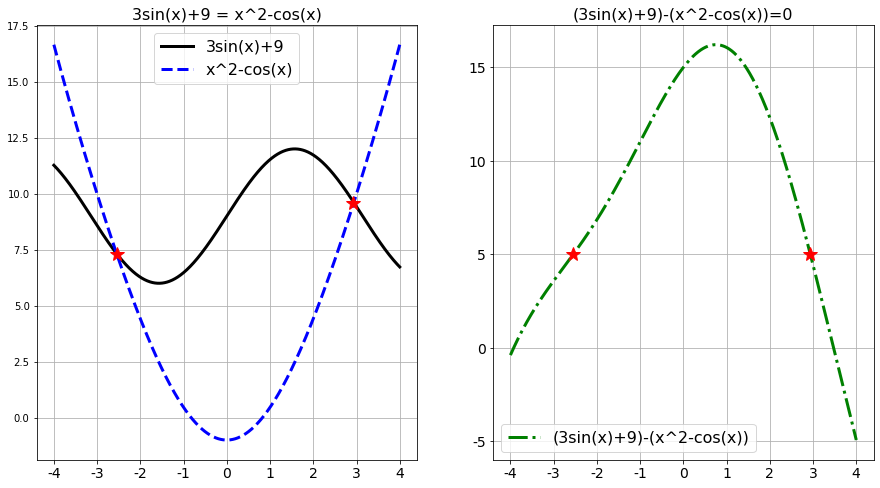
\includegraphics[width=0.9\linewidth]{images/Ch02Sec01_IntroRootFinding} 

}

\caption{A Typical Root Finding Problem}\label{fig:root-finding-intro}
\end{figure}

On the left-hand side of Figure \ref{fig:root-finding-intro} we see the solutions to the equation \(3\sin(x) + 9 = x^2 - \cos(x)\), and on the right-hand side we see the solutions to the equation
\[ \left( 3\sin(x)+9 \right) - \left( x^2 - \cos(x) \right) = 0.\]
From the plots it is apparent that the two equations have the same solutions: \(x_1 \approx -2.55\) and \(x_2 \approx 2.88\). This plot should demonstrate what we me when we say that solving equations of the form \(\ell(x) = r(x)\) will give the same answer and solving \(f(x) = 0\).

We now have one way to view every algebraic equation-solving problem. As we'll see in this chapter, if \(f(x)\) has certain properties then different numerical techniques for solving the equation will apply -- and some will be much faster and more accurate than others. The following sections give several different techniques for solving algebraic equations of the form \(f(x) = 0\). We will start with the simplest techniques to implement and then move to the more powerful techniques that require some ideas from Calculus to understand and analyze. Throughout this chapter we will also work to quantify the amount of error that we make while using these techniques.

\hypertarget{the-bisection-method}{%
\section{The Bisection Method}\label{the-bisection-method}}

\hypertarget{intuition-and-implementation}{%
\subsection{Intuition and Implementation}\label{intuition-and-implementation}}

\begin{exercise}
\protect\hypertarget{exr:bisection1}{}{\label{exr:bisection1} }A friend tells you that she is thinking of a number between 1 and 100. She will allow you multiple guesses with some feedback for where the mystery number falls. How do you systematically go about guessing the mystery number? Is there an optimal strategy?

For example, the conversation might go like this.

\begin{itemize}
\tightlist
\item
  Sally: I'm thinking of a number between 1 and 100
\item
  Joe: Is it 35?
\item
  Sally: No, but the number is between 35 and 100
\item
  Joe: Is it 99?
\item
  Sally: No, but the number is between 35 and 99
\item
  \ldots{}
\end{itemize}
\end{exercise}

\begin{center}\rule{0.5\linewidth}{0.5pt}\end{center}

\begin{exercise}
\protect\hypertarget{exr:bisection2}{}{\label{exr:bisection2} }Now let's say that Sally has a continuous function that has a root somewhere between \(x=2\) and \(x=10\). Modify your strategy from the number guessing game in the previous problem to narrow down where the root is.
\end{exercise}

\begin{center}\rule{0.5\linewidth}{0.5pt}\end{center}

\begin{exercise}
\protect\hypertarget{exr:unnamed-chunk-70}{}{\label{exr:unnamed-chunk-70} }Was it necessary to say that Sally's function was continuous? Could your technique work if the function were not continuous.
\end{exercise}

\begin{center}\rule{0.5\linewidth}{0.5pt}\end{center}

Now let's get to the math. We'll start the mathematical discussion with a theorem from Calculus.

\begin{theorem}[The Intermediate Value Theorem (IVT)]
\protect\hypertarget{thm:unnamed-chunk-71}{}{\label{thm:unnamed-chunk-71} \iffalse (The Intermediate Value Theorem (IVT)) \fi{} }If \(f(x)\) is a continuous function on the closed interval \([a,b]\) and
\(y_*\) lies between \(f(a)\) and \(f(b)\), then there exists some point
\(x_* \in [a,b]\) such that \(f(x_*) = y_*\).
\end{theorem}

\begin{center}\rule{0.5\linewidth}{0.5pt}\end{center}

\begin{exercise}
\protect\hypertarget{exr:unnamed-chunk-72}{}{\label{exr:unnamed-chunk-72} }Draw a picture of what the intermediate value theorem says graphically.
\end{exercise}

\begin{center}\rule{0.5\linewidth}{0.5pt}\end{center}

\begin{exercise}
\protect\hypertarget{exr:unnamed-chunk-73}{}{\label{exr:unnamed-chunk-73} }If \(y_*=0\) the Intermediate Value Theorem gives us important information
about solving equations. What does it tell us?
\end{exercise}

\begin{center}\rule{0.5\linewidth}{0.5pt}\end{center}

\begin{corollary}
\protect\hypertarget{cor:unnamed-chunk-74}{}{\label{cor:unnamed-chunk-74} }If \(f(x)\) is a continuous function on the closed interval \([a,b]\) and if
\(f(a)\) and \(f(b)\) have opposite signs then from the Intermediate Value
Theorem we know that there exists some point \(x_* \in [a,b]\) such that \_\_\_\_.
\end{corollary}

\begin{center}\rule{0.5\linewidth}{0.5pt}\end{center}

\begin{exercise}
\protect\hypertarget{exr:unnamed-chunk-75}{}{\label{exr:unnamed-chunk-75} }Fill in the blank in the previous corollary and then draw several pictures that indicate why this might be true for continuous functions.
\end{exercise}

\begin{center}\rule{0.5\linewidth}{0.5pt}\end{center}

The Intermediate Value Theorem (IVT) and its corollary are \emph{existence theorems} in the
sense that they tell us that some point exists. The annoying thing about
mathematical existence theorems is that they typically don't tell us
\emph{how} to find the point that is guaranteed to exist -- annoying. The method that you developed in Exercises \ref{exr:bisection1} and \ref{exr:bisection2} give one possible way to find the root.

In Exercises \ref{exr:bisection1} and \ref{exr:bisection2} you likely came up with an algorithm such as this:

\begin{itemize}
\tightlist
\item
  Say we know that the root of a continuous function lies between \(x=a\) and \(x=b\).
\item
  Guess that the root is at the midpoint \(m = \frac{a+b}{2}\).
\item
  By using the signs of the function narrow the interval which contains the root to either \([a,m]\) or \([m,b]\).
\item
  Repeat
\end{itemize}

Now we will turn this optimal strategy into computer code that will simply play the game for us. But first we need to pay careful attention to some of the mathematical details.

\begin{center}\rule{0.5\linewidth}{0.5pt}\end{center}

\begin{exercise}
\protect\hypertarget{exr:unnamed-chunk-76}{}{\label{exr:unnamed-chunk-76} }Where is the Intermediate Value Theorem used in the root-guessing strategy?
\end{exercise}

\begin{center}\rule{0.5\linewidth}{0.5pt}\end{center}

\begin{exercise}
\protect\hypertarget{exr:unnamed-chunk-77}{}{\label{exr:unnamed-chunk-77} }Why was it important that the function \(f(x)\) is continuous when playing this root-guessing game? Provide a few sketches to demonstrate your answer.
\end{exercise}

\begin{center}\rule{0.5\linewidth}{0.5pt}\end{center}

\begin{exercise}[The Bisection Method]
\protect\hypertarget{exr:unnamed-chunk-78}{}{\label{exr:unnamed-chunk-78} \iffalse (The Bisection Method) \fi{} }\textbf{Goal:} We want to solve the algebraic equation \(f(x) = 0\) for \(x\) assuming that the solution \(x^*\) is in the interval \([a,b]\).

\textbf{The Algorithm:} Assume that \(f(x)\) is continuous on the closed interval \([a,b]\). To make
approximations of the solutions to the equation \(f(x) = 0\), do the
following:

\begin{enumerate}
\def\labelenumi{\arabic{enumi}.}
\item
  Check to see if \(f(a)\) and \(f(b)\) have opposite signs. You can do
  this taking the product of \(f(a)\) and \(f(b)\).

  \begin{itemize}
  \item
    If \(f(a)\) and \(f(b)\) have different signs then what does the IVT
    tell you?
  \item
    If \(f(a)\) and \(f(b)\) have the same sign then what does the IVT
    not tell you? What should you do in this case?
  \item
    Why does the product of \(f(a)\) and \(f(b)\) tell us something
    about the signs of the two numbers?
  \end{itemize}
\item
  Compute the midpoint of the closed interval, \(m=\frac{a+b}{2}\), and
  evaluate \(f(m)\).

  \begin{itemize}
  \item
    Will \(m\) always be a better guess of the root than \(a\) or \(b\)?
    Why?
  \item
    What should you do here if \(f(m)\) is really close to zero?
  \end{itemize}
\item
  Compare the signs of \(f(a)\) vs \(f(m)\) and \(f(b)\) vs \(f(m)\).

  \begin{itemize}
  \item
    What do you do if \(f(a)\) and \(f(m)\) have opposite signs?
  \item
    What do you do if \(f(m)\) and \(f(b)\) have opposite signs?
  \end{itemize}
\item
  Repeat steps 2 and 3 and stop when \(f(m)\) is \emph{close enough} to zero.
\end{enumerate}
\end{exercise}

\begin{center}\rule{0.5\linewidth}{0.5pt}\end{center}

\begin{exercise}
\protect\hypertarget{exr:unnamed-chunk-79}{}{\label{exr:unnamed-chunk-79} }Draw a picture illustrating what the Bisection Method does to
approximate solutions to the algebraic equation \(f(x) = 0\).
\end{exercise}

\begin{center}\rule{0.5\linewidth}{0.5pt}\end{center}

\begin{exercise}
\protect\hypertarget{exr:unnamed-chunk-80}{}{\label{exr:unnamed-chunk-80} }We want to write a Python function for the Bisection Method. Instead of jumping
straight into the code we should ALWAYS write pseudo-code first. It is
often helpful to write pseudo-code as comments in your file. Use the
template below to complete your pseudo-code.
\end{exercise}

\begin{Shaded}
\begin{Highlighting}[]
\KeywordTok{def}\NormalTok{ Bisection(f , a , b , tol):}
\CommentTok{\# The input parameters are}
\CommentTok{\# f is a Python function or a lambda function}
\CommentTok{\# a is the lower guess}
\CommentTok{\# b is the upper guess}
\CommentTok{\# tol is an optional tolerance for the accuracy of the root}

\CommentTok{\# if the user doesn\textquotesingle{}t define a tolerance we need code to create a default}

\CommentTok{\# check that there is a root between a and b}
\CommentTok{\# if not we should return an error and break the code}

\CommentTok{\# next calculate the midpoint m = (a+b)/2}

\CommentTok{\# start a while loop}
\CommentTok{\#   \# in the while loop we need an if statement}
\CommentTok{\#   \# if ...}
\CommentTok{\#   \# elif ...}
\CommentTok{\#   \# elif ...}

\CommentTok{\#   \# we should check that the while loop isn\textquotesingle{}t running away}

\CommentTok{\# end the while loop}
\CommentTok{\# define and return the root}
\end{Highlighting}
\end{Shaded}

\begin{center}\rule{0.5\linewidth}{0.5pt}\end{center}

\begin{exercise}
\protect\hypertarget{exr:unnamed-chunk-82}{}{\label{exr:unnamed-chunk-82} }Now use the pseudo-code as structure to complete a function for the
Bisection Method. Also write test code that verifies that your
function works properly. Be sure that it can take a Lambda Function as an input along with an initial lower
bound, an initial upper bound, and an optional error tolerance. The
output should be only 1 single number: the root.
\end{exercise}

\begin{center}\rule{0.5\linewidth}{0.5pt}\end{center}

\begin{exercise}
\protect\hypertarget{exr:unnamed-chunk-83}{}{\label{exr:unnamed-chunk-83} }Test your Bisection Method code on the following algebraic equations.

\begin{enumerate}
\def\labelenumi{\alph{enumi}.}
\tightlist
\item
  \(x^2 - 2 = 0\) on \(x \in [0,2]\)
\item
  \(\sin(x) + x^2 = 2\ln(x) + 5\) on \(x \in [0,5]\) (be careful! make a
  plot first)
\item
  \((5-x)e^{x}=5\) on \(x \in [0,5]\)
\end{enumerate}
\end{exercise}

\begin{center}\rule{0.5\linewidth}{0.5pt}\end{center}

\hypertarget{analysis}{%
\subsection{Analysis}\label{analysis}}

After we build any root finding algorithm we need to stop and think about how it will perform on new problems. The questions that we typically have for a root-finding algorithm are:

\begin{itemize}
\tightlist
\item
  Will the algorithm always converge to a solution?
\item
  How fast will the algorithm converge to a solution?
\item
  Are there any pitfalls that we should be aware of when using the algorithm?
\end{itemize}

\begin{center}\rule{0.5\linewidth}{0.5pt}\end{center}

\begin{exercise}
\protect\hypertarget{exr:unnamed-chunk-84}{}{\label{exr:unnamed-chunk-84} }Discussion: What must be true in order to use the bisection method?
\end{exercise}

\begin{center}\rule{0.5\linewidth}{0.5pt}\end{center}

\begin{exercise}
\protect\hypertarget{exr:unnamed-chunk-85}{}{\label{exr:unnamed-chunk-85} }Discussion: Does the bisection method work if the Intermediate Value Theorem does not apply? (Hint: what does it mean for the IVT to ``not apply''?)
\end{exercise}

\begin{center}\rule{0.5\linewidth}{0.5pt}\end{center}

\begin{exercise}
\protect\hypertarget{exr:unnamed-chunk-86}{}{\label{exr:unnamed-chunk-86} }If there is a root of a continuous function \(f(x)\) between \(x=a\) and \(x=b\) will the bisection method always be able to find it? Why / why not?
\end{exercise}

\begin{center}\rule{0.5\linewidth}{0.5pt}\end{center}

Next we'll focus on a deeper mathematical analysis that will allow us to determine exactly how fast the bisection method actually converges to within a pre-set tolerance. Work through the next problem to develop a formula that tells you exactly how many steps the bisection method needs to take in order to stop.

\begin{center}\rule{0.5\linewidth}{0.5pt}\end{center}

\begin{exercise}
\protect\hypertarget{exr:bisectionerror}{}{\label{exr:bisectionerror} }Let \(f(x)\) be a continuous function on the interval \([a,b]\) and assume
that \(f(a) \cdot f(b) <0\). A reoccurring theme in Numerical Analysis is to
approximate some mathematical thing to within some tolerance. For
example, if we want to approximate the solution to the equation \(f(x)=0\)
to within \(\varepsilon\) with the bisection method, we should be able to
figure out how many steps it will take to achieve that goal.

\begin{enumerate}
\def\labelenumi{\alph{enumi}.}
\item
  Let's say that \(a = 3\) and \(b = 8\) and \(f(a) \cdot f(b) < 0\) for
  some continuous function \(f(x)\). The width of this interval is 5, so
  if we guess that the root is \(m=(3+8)/2 = 5.5\) then our error is
  less than \(5/2\). In the more general setting, if there is a root of
  a continuous function in the interval \([a,b]\) then how far off could
  the midpoint approximation of the root be? In other words, what is
  the error in using \(m=(a+b)/2\) as the approximation of the root?
\item
  The bisection method cuts the width of the interval down to a
  smaller size at every step. As such, the approximation error gets
  smaller at every step. Fill in the blanks in the following table to
  see the pattern in how the approximation error changes with each
  iteration.
\end{enumerate}

\begin{longtable}[]{@{}lll@{}}
\toprule
Iteration & Width of Interval & Approximation Error\tabularnewline
\midrule
\endhead
0 & \(|b-a|\) & \(\frac{|b-a|}{2}\)\tabularnewline
1 & \(\frac{|b-a|}{2}\) &\tabularnewline
2 & \(\frac{|b-a|}{2^2}\) &\tabularnewline
\(\vdots\) & \(\vdots\) & \(\vdots\)\tabularnewline
\(n\) & \(\frac{|b-a|}{2^n}\) &\tabularnewline
\bottomrule
\end{longtable}

\begin{enumerate}
\def\labelenumi{\alph{enumi}.}
\setcounter{enumi}{2}
\tightlist
\item
  Now to the key question:\\
  If we want to approximate the solution to the equation \(f(x)=0\) to
  within some tolerance \(\varepsilon\) then how many iterations of the
  bisection method do we need to take?\\
  Hint: Set the \(n^{th}\) approximation error from the table equal to
  \(\varepsilon\). What should you solve for from there?
\end{enumerate}
\end{exercise}

\begin{center}\rule{0.5\linewidth}{0.5pt}\end{center}

In Exercise \ref{exr:bisectionerror} you actually proved the following theorem.

\begin{theorem}[Convergence Rate of the Bisection Method]
\protect\hypertarget{thm:bisectionconvergence}{}{\label{thm:bisectionconvergence} \iffalse (Convergence Rate of the Bisection Method) \fi{} }If \(f(x)\) is a continuous function with a root in the interval \([a,b]\) and if the bisection method is performed to find the root then:

\begin{itemize}
\tightlist
\item
  The error between the actual root and the approximate root will decrease by a factor of 2 at every iteration.
\item
  If we want the approximate root found by the bisection method to be within a tolerance of \(\varepsilon\) then
  \[ \frac{|b-a|}{2^{n+1}} = \varepsilon \]
  where \(n\) is the number of iterations that it takes to achieve that tolerance.

  \begin{itemize}
  \tightlist
  \item
    Solving for the number of iterations (\(n\)) we get
    \[ n = \log_2\left( \frac{|b-a|}{\varepsilon} \right) - 1. \]
  \item
    Rounding the value of \(n\) up to the nearest integer gives the number of iterations necessary to approximate the root to a precision less than \(\varepsilon\).
  \end{itemize}
\end{itemize}
\end{theorem}

\begin{center}\rule{0.5\linewidth}{0.5pt}\end{center}

\begin{exercise}
\protect\hypertarget{exr:unnamed-chunk-87}{}{\label{exr:unnamed-chunk-87} }Is it possible for a given function and a given interval that the
Bisection Method converges to the root in fewer steps than what you just
found in the previous problem? Explain.
\end{exercise}

\begin{center}\rule{0.5\linewidth}{0.5pt}\end{center}

\begin{exercise}
\protect\hypertarget{exr:unnamed-chunk-88}{}{\label{exr:unnamed-chunk-88} }Create a second version of your Python Bisection Method function that uses a \texttt{for}
loop that takes the optimal number of steps to approximate the root to
within some tolerance. This should be in contrast to your first version
which likely used a \texttt{while} loop to decide when to stop. Is there an advantage
to using one of these version of the Bisection Method over the other?
\end{exercise}

\begin{center}\rule{0.5\linewidth}{0.5pt}\end{center}

The final type of analysis that we should do on the bisection method is to make plots of the error between the approximate solution that the bisection method gives you and the exact solution to the algebraic equation. This is a bit of a funny thing! Stop and think about this for a second: \emph{if you know the exact solution to the equation then why are you solving it numerically in the first place!?!?} However, whenever you build an algorithm you need to test it on problems where you actually do know the answer so that you can can be somewhat sure that it isn't giving you nonsense. Furthermore, analysis like this tells us how fast the algorithm is expected to perform.

From Theorem \ref{thm:bisectionconvergence} you know that the bisection method cuts the interval in half at every iteration. You proved in Exercise \ref{exr:bisectionerror} that the error given by the bisection method is therefore cut in half at every iteration as well. The following example demonstrate this theorem graphically.

\begin{center}\rule{0.5\linewidth}{0.5pt}\end{center}

\begin{example}
\protect\hypertarget{exm:bisectionplots}{}{\label{exm:bisectionplots} }Let's solve the very simple algebraic problem \(x^2 - 2 = 0\) for \(x\) to get the solution \(x = \sqrt{2}\) with the bisection method. Since we know the exact answer we can compare the exact answer to the value of the midpoint given at each iteration and calculate an absolute error:
\[ \text{Absolute Error} = | \text{Approximate Solution} - \text{Exact Solution}|. \]

\begin{enumerate}
\def\labelenumi{\alph{enumi}.}
\tightlist
\item
  If we plot the absolute error on the vertical axis and the iteration number on the horizontal axis we get Figure \ref{fig:bisection-exponential-error}. As expected, the absolute error follows an exponentially decreasing trend. Notice that it isn't a completely smooth curve since we will have some jumps in the accuracy just due to the face that sometimes the root will be near the midpoint of the interval and sometimes it won't be.
\end{enumerate}
\end{example}

\begin{figure}

{\centering 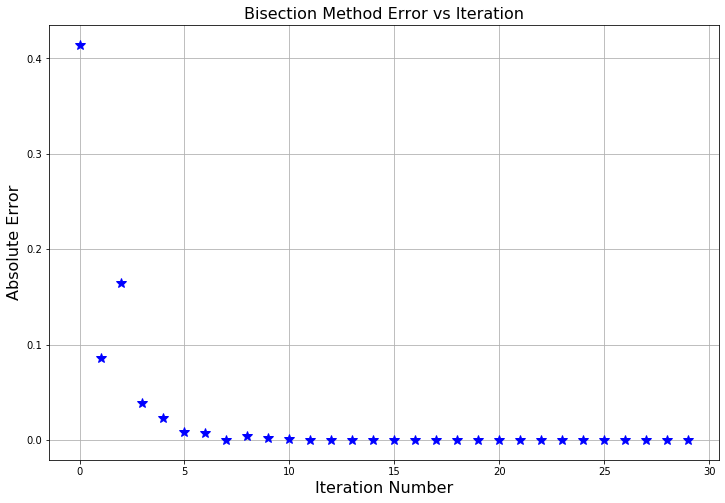
\includegraphics[width=0.9\linewidth]{images/Ch02Sec02_BisectionError1} 

}

\caption{The evolution of the absolute error when solving the equation $x^2-2=0$ with the bisection method.}\label{fig:bisection-exponential-error}
\end{figure}

\begin{enumerate}
\def\labelenumi{\alph{enumi}.}
\setcounter{enumi}{1}
\tightlist
\item
  Without Theorem \ref{thm:bisectionconvergence} it would be rather hard to tell what the exact behavior is in the exponential plot above. We know from Theorem \ref{thm:bisectionconvergence} that the error will divide by 2 at every step, so if we instead plot the base-2 logarithm of the absolute error against the iteration number we should see a linear trend as shown in Figure \ref{fig:bisection-error-1}. There will be times later in this course where we won't have a nice theorem like Theorem \ref{thm:bisectionconvergence} and instead we will need to deduce the relationship from plots like these.

  \begin{enumerate}
  \def\labelenumii{\roman{enumii}.}
  \tightlist
  \item
    The trend is linear since logarithms and exponential functions are inverses. Hence, applying a logarithm to an exponential will give a linear function.
  \item
    The slope of the resulting linear function should be \(-1\) in this case since we are dividing by 1 power of 2 each iteration. Visually verify that the slope in the plot below follows this trend (the red dashed line in the plot is shown to help you see the slope).
  \end{enumerate}
\end{enumerate}

\begin{figure}

{\centering 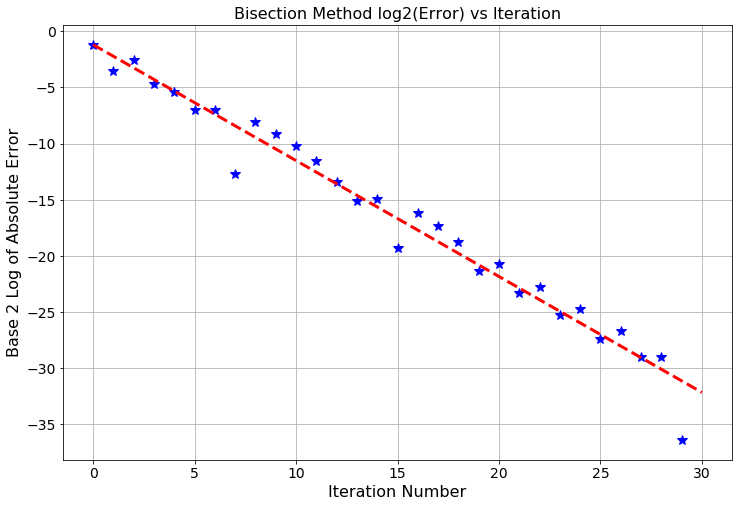
\includegraphics[width=0.75\linewidth]{images/Ch02Sec02_BisectionError2} 

}

\caption{Iteration number vs the base-2 logarithm of the absolute error.  Notice the slope of $-1$ indicating that the error is divided by 1 factor of 2 at each step of the algorithm.}\label{fig:bisection-error-1}
\end{figure}

\begin{enumerate}
\def\labelenumi{\alph{enumi}.}
\setcounter{enumi}{2}
\tightlist
\item
  Another plot that numerical analysts use quite frequently for determining how an algorithm is behaving as it progresses is described by the following bullets:
\end{enumerate}

\begin{itemize}
\tightlist
\item
  The horizontal axis is the absolute error at iteration \(k\).
\item
  The vertical axis is the absolute error at iteration \(k+1\).
\end{itemize}

See Figure \ref{fig:bisection-error-2} below, but this type of plot takes a bit of explaining the first time you see it. Start on the right-hand side of the plot where the error is the largest (this will be where the algorithm starts). The coordinates of the first point are interpreted as:
\[ (\text{absolute error at step 1} \, , \, \text{absolute error at step 2}). \]
The coordinates of the second point are interpreted as:
\[ (\text{absolute error at step 2} \, , \, \text{absolute error at step 3}). \]
Etc. Examining the slope of the trend line in this plot shows how we expect the error to progress from step to step. The slope appears to be about \(1\) in the plot below and the intercept appears to be about \(-1\). In this case we used a base-2 logarithm for each axis so we have just empirically shown that
\[ \log_2(\text{absolute error at step $k+1$}) \approx 1\cdot \log_2(\text{absolute error at step $k$}) -1. \]
Rearranging the algebra a bit we see that this linear relationship turns into
\[ \frac{\text{absolute error at step $k+1$}}{\text{absolute error at step $k$}} \approx \frac{1}{2}. \]
(You should stop now and do this algebra.) Rearranging a bit more we get
\[ (\text{absolute error at step $k+1$}) = \frac{1}{2}(\text{absolute error at step $k$}), \]
exactly as expected!! Pause and ponder this result for a second -- we just empirically verified the convergence rate for the bisection method just by examining the plot below!! That's what makes these types of plots so powerful!

\begin{figure}

{\centering 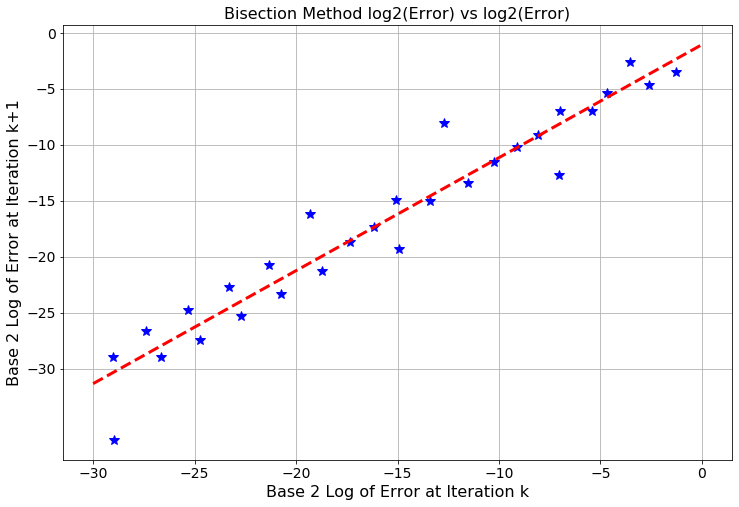
\includegraphics[width=0.75\linewidth]{images/Ch02Sec02_BisectionError3} 

}

\caption{The base-2 logarithm of the absolute error at iteration $k$ vs the base-2 logarithm of the absolute error at iteration $k+1$.}\label{fig:bisection-error-2}
\end{figure}

\begin{enumerate}
\def\labelenumi{\alph{enumi}.}
\setcounter{enumi}{3}
\tightlist
\item
  The final plot that we will make in analyzing the bisection method is the same as the plot that we just made but with the base-10 logarithm instead. See Figure \ref{fig:bisection-error-3}. In future algorithms we will not know that the error decreases by a factor of 2 so instead we will just try the base-10 logarithm. We will be able to extract the exact same information from this plot. The primary advantage of this last plot is that we can see how the order of magnitude (the power of 10) for the error progresses as the algorithm steps forward. Notice that
\end{enumerate}

\begin{figure}

{\centering 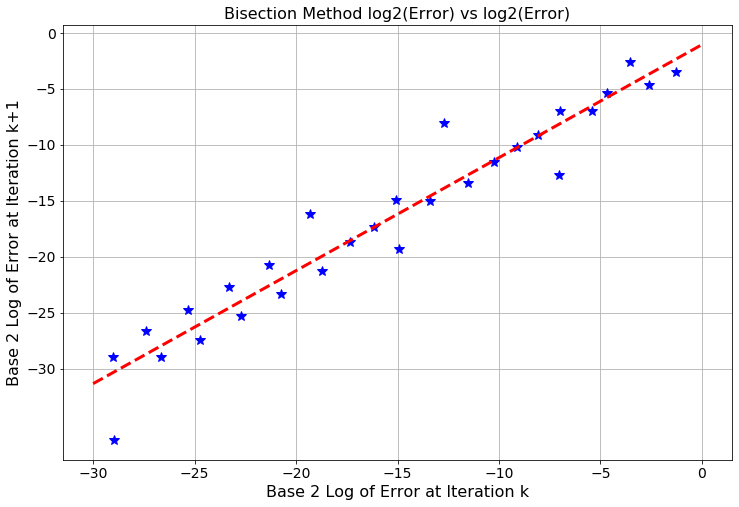
\includegraphics[width=0.75\linewidth]{images/Ch02Sec02_BisectionError3} 

}

\caption{The base-10 logarithm of the absolute error at iteration $k$ vs the base-10 logarithm of the absolute error at iteration $k+1$.}\label{fig:bisection-error-3}
\end{figure}

\begin{center}\rule{0.5\linewidth}{0.5pt}\end{center}

\begin{exercise}
\protect\hypertarget{exr:unnamed-chunk-89}{}{\label{exr:unnamed-chunk-89} }Carefully read and discuss all of the details of the previous example and plots. Then create plots similar to this example to solve an algebraic equation to which you know the exact solution to. You should see the same basic behavior based on the theorem that you proved in Exercise \ref{exr:bisectionerror}. If you don't see the same basic behavior then something has gone wrong.

\begin{description}
\item[Hints:]
You will need to create a modified bisection method function which returns all of the iterations instead of just the final root.

If the logarithms of your absolute errors are in a Python list called \texttt{error} then a command like \texttt{plt.plot(error{[}0:-2{]},error{[}1:-1{]},\textquotesingle{}b*\textquotesingle{})} will plot the \((k+1)^{st}\) absolute error against the \(k^{th}\) absolute error.

If you want the actual slope and intercept of the trend line then you can use \texttt{m,\ b\ =\ np.polyfit(error{[}0:-2{]},\ error{[}1:-1{]},\ deg=1)}.
\end{description}
\end{exercise}

\begin{center}\rule{0.5\linewidth}{0.5pt}\end{center}

\hypertarget{the-regula-falsi-method}{%
\section{The Regula Falsi Method}\label{the-regula-falsi-method}}

\hypertarget{intuition-and-implementation-1}{%
\subsection{Intuition and Implementation}\label{intuition-and-implementation-1}}

The bisection method is one of many methods for performing root finding
on a continuous function. The next algorithm takes a slightly different
approach.

\begin{center}\rule{0.5\linewidth}{0.5pt}\end{center}

\begin{exercise}
\protect\hypertarget{exr:unnamed-chunk-90}{}{\label{exr:unnamed-chunk-90} }In the Bisection Method, we always used the midpoint of the interval as
the next approximation of the root of the function \(f(x)\) on the
interval \([a,b]\). The three pictures in Figure \ref{fig:regula-falsi-1} show the same function
with three different choices for \(a\) and \(b\). Which one will take fewer
Bisection-steps to find the root? Which one will take more steps? Explain your reasoning.

(\emph{Note: The root in question is marked with the green star and the initial interval is marked with the red circles.})
\end{exercise}

\begin{figure}

{\centering 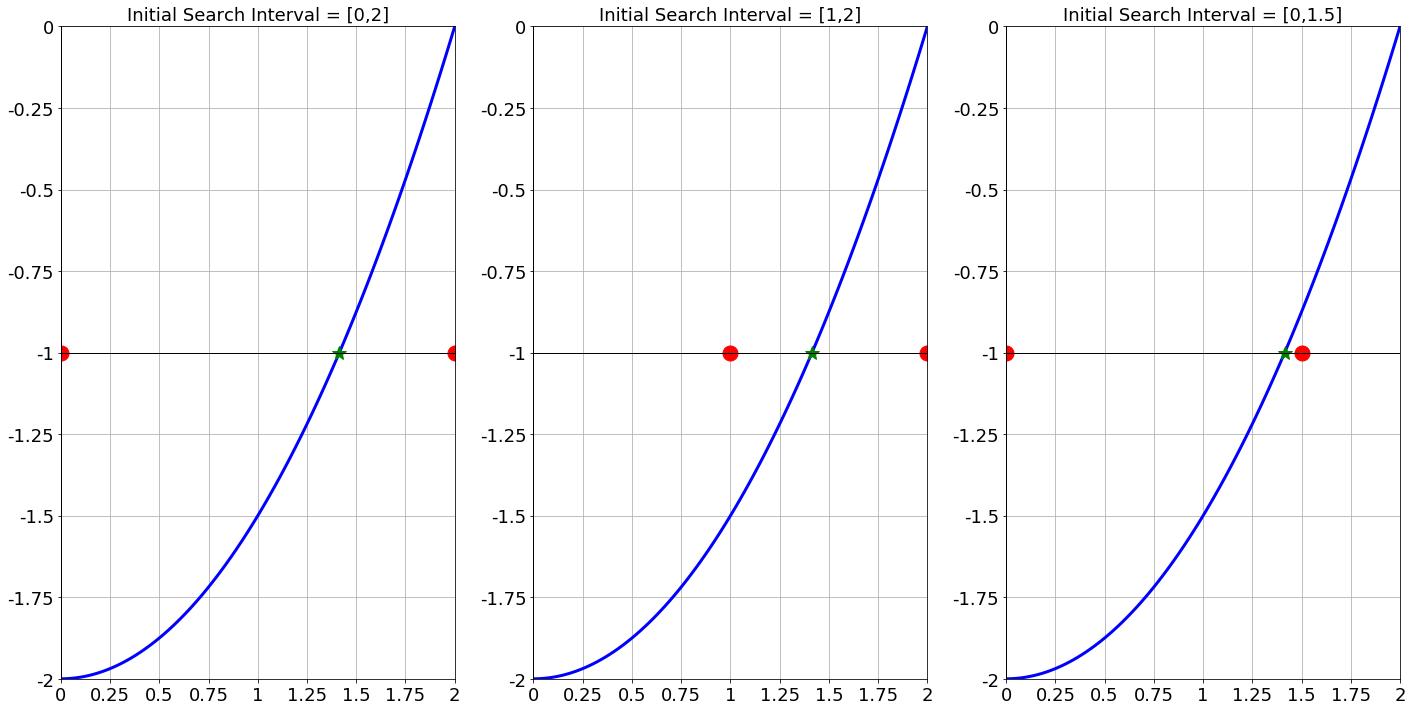
\includegraphics[width=0.75\linewidth]{images/Ch02Sec03_MultipleBisections} 

}

\caption{In the bisection method you get to choose the starting interval however you like.  That choice will make an impact on how fast the algorithm converges to the approximate root.}\label{fig:regula-falsi-1}
\end{figure}

\begin{center}\rule{0.5\linewidth}{0.5pt}\end{center}

\begin{exercise}
\protect\hypertarget{exr:unnamed-chunk-91}{}{\label{exr:unnamed-chunk-91} }Now let's modify the Bisection Method approach. Instead of always using
the midpoint (which as you saw in the previous problem could take a
little while to converge) let's draw a line between the endpoints and
use the \(x\)-intercept as the updated guess. If we use this method can we
improve the speed of convergence on any of the choices of \(a\) and \(b\)
for this function? Which one will now likely take the fewest steps to
converge? Figure \ref{fig:regula-falsi-2} shows three different starting intervals marked in red with the new guess marked as a black X.
\end{exercise}

\begin{figure}

{\centering 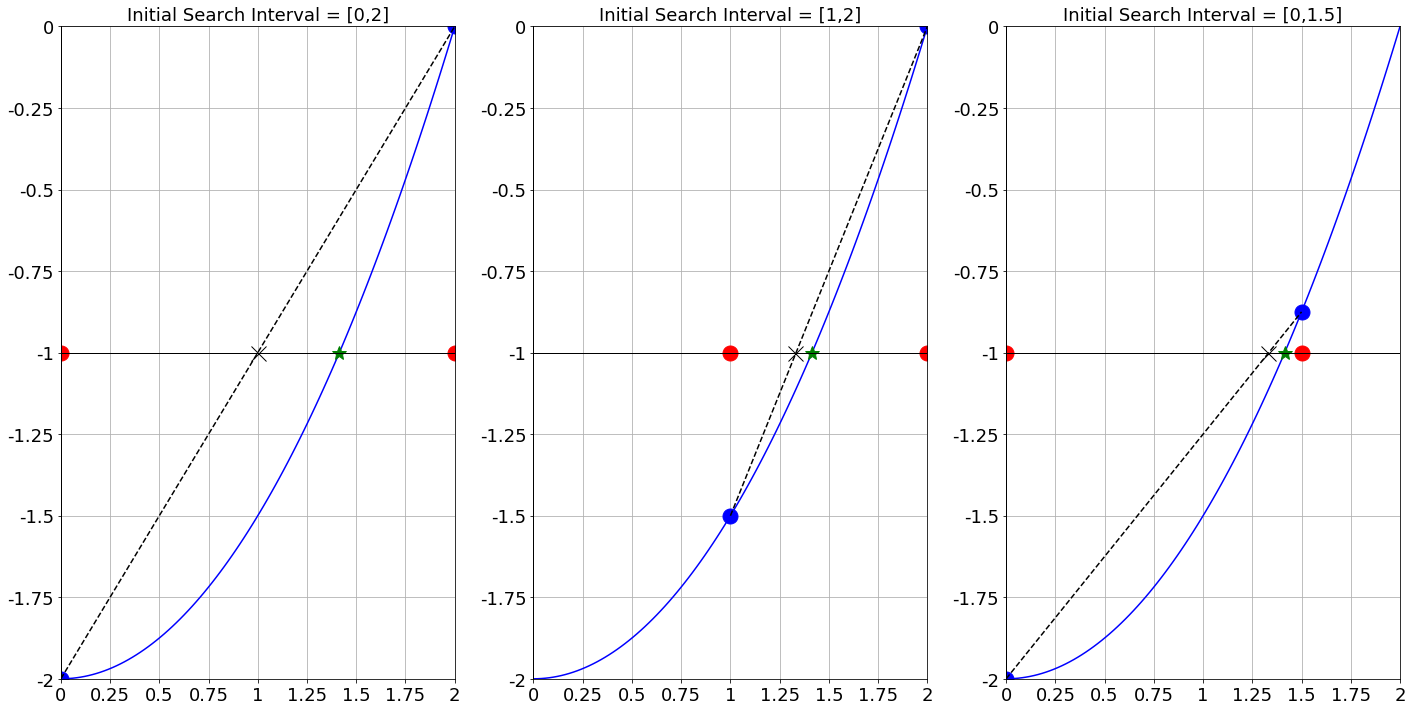
\includegraphics[width=0.75\linewidth]{images/Ch02Sec03_MultipleBisections2} 

}

\caption{In hopes of improving the bisection method we instead propose that we choose the intersection of a line between the endpoints of the interval and the $x$ axis.  The intersection (marked with a black X) would be the next approximation instead of the midpoint of the interval.}\label{fig:regula-falsi-2}
\end{figure}

\begin{center}\rule{0.5\linewidth}{0.5pt}\end{center}

The algorithm that you played with graphically in the previous problem
is known as the Regula Falsi (false position) algorithm. It is really
just a minor tweak on the Bisection method. After all, the algorithm is
still designed to use the Intermediate Value Theorem and to iteratively
zero in on the root of the function on the given interval. This time, instead of picking the midpoint of the interval that contains the root we draw a line between the function values at either end of the interval and then use the intersection of that line with the \(x\) axis as the new approximation of the root. As you can see in Figure \ref{fig:regula-falsi-2} you might actually converge to the approximate root much faster this way (like with the far right plot) or you might gain very little performance (like the far left plot).

\begin{center}\rule{0.5\linewidth}{0.5pt}\end{center}

\begin{exercise}[The Regula Falsi Method]
\protect\hypertarget{exr:regula-falsi}{}{\label{exr:regula-falsi} \iffalse (The Regula Falsi Method) \fi{} }Assume that \(f(x)\) is continuous on the interval \([a,b]\). To make iterative
approximations of the solutions to the equation \(f(x) = 0\), do the
following:

\begin{enumerate}
\def\labelenumi{\arabic{enumi}.}
\item
  Check to see if \(f(a)\) and \(f(b)\) have opposite signs so that the
  intermediate value theorem guarantees a root on the interval.
\item
  We want to write the equation of the line connecting the points
  \((a,f(a))\) and \((b,f(b))\).

  \begin{itemize}
  \item
    What is the slope of this line? \[m = \underline{\hspace{0.4in}}\]
  \item
    Using the point-slope form of a line, \(y-y_1 = m(x-x_1)\), what
    is the equation of the line?
    \[y - \underline{\hspace{0.4in}} = \underline{\hspace{0.4in}} \cdot
                        \left( x - \underline{\hspace{0.4in}} \right)\]
  \end{itemize}
\item
  Find the \(x\) intercept of the linear function that you wrote in the
  previous step by setting the \(y\) to zero and solving for \(x\). Call
  this point \(x=c\). \[c = \underline{\hspace{2in}}\]
  \emph{Hint: The \(x\) intercept occurs with \(y=0\).}
\item
  Just as we did with the bisection method, compare the signs of
  \(f(a)\) vs \(f(c)\) and \(f(b)\) vs \(f(c)\). Replace one of the endpoints
  with \(c\). Which one do you replace and why?
\item
  Repeat steps 2 - 4, and stop when \(f(c)\) is \emph{close enough} to zero.
\end{enumerate}
\end{exercise}

\begin{center}\rule{0.5\linewidth}{0.5pt}\end{center}

\begin{exercise}
\protect\hypertarget{exr:unnamed-chunk-92}{}{\label{exr:unnamed-chunk-92} }Draw a picture of what the Regula Falsi method does to approximate a
root.
\end{exercise}

\begin{center}\rule{0.5\linewidth}{0.5pt}\end{center}

\begin{exercise}
\protect\hypertarget{exr:unnamed-chunk-93}{}{\label{exr:unnamed-chunk-93} }Give sketches of functions where the Regula Falsi method will perform
faster than the Bisection method and visa versa. Justify your thinking
with several pictures and be prepared to defend your answers.
\end{exercise}

\begin{center}\rule{0.5\linewidth}{0.5pt}\end{center}

\begin{exercise}
\protect\hypertarget{exr:regulafalsi-python}{}{\label{exr:regulafalsi-python} }Create a new Python function called \texttt{regulafalsi} and write comments giving pseudo-code for
the Regula-Falsi method. Remember that starting with pseudo-code is always the best way to start your coding. Write comments that give direction to the code that you're about to write. It is a trap to try and write actual code without any pseudo-code to give you a backbone for the function.
\end{exercise}

\begin{center}\rule{0.5\linewidth}{0.5pt}\end{center}

\begin{exercise}
\protect\hypertarget{exr:unnamed-chunk-94}{}{\label{exr:unnamed-chunk-94} }Use your pseudo-code to create a Python function that implements the Regula
Falsi method. Write a test script that verifies that your function
works properly. Your function should accept a Python function or a Lambda function as input along with
an initial lower bound, an
initial upper bound, and an optional error tolerance. The output should
be only 1 single number: the approximate root.
\end{exercise}

\begin{center}\rule{0.5\linewidth}{0.5pt}\end{center}

\hypertarget{analysis-1}{%
\subsection{Analysis}\label{analysis-1}}

In this subsection we will lean on the fact that we developed a bunch of analysis tools in the Analysis section of the Bisection Method. You may want to go back to that section first and take another look at the plots and tools that we built.

\begin{center}\rule{0.5\linewidth}{0.5pt}\end{center}

\begin{exercise}
\protect\hypertarget{exr:unnamed-chunk-95}{}{\label{exr:unnamed-chunk-95} }In this problem we are going to solve the algebraic equation \(x^2 - 2 = 0\) since we know that the exact answer is \(x = \sqrt{2}\). You will need to start by modifying your \texttt{regulafalsi} function from Exercise \ref{exr:regulafalsi-python} so that it returns all of the iterations instead of just the root.

\begin{enumerate}
\def\labelenumi{\alph{enumi}.}
\tightlist
\item
  Start with the interval \([0,2]\) and solve the equation \(x^2 - 2 = 0\) with the Regula-Falsi method.

  \begin{enumerate}
  \def\labelenumii{\roman{enumii}.}
  \tightlist
  \item
    Find the absolute error between each iteration and the exact answer \(x=\sqrt{2}\).
  \item
    Make a plot of the base-10 logarithm of the absolute error at step \(k\) against the base-10 logarithm of the absolute error at step \(k+1\). This plot will be very similar to Figure \ref{fig:bisection-error-3}.
  \item
    Approximate the slope and intercept of the linear trend in the plot.
    \[ \log_{10}(\text{abs error at step $k+1$}) = \underline{\hspace{0.4in}} \log_{10}(\text{abs error at step $k+1$}) + \underline{\hspace{0.4in}} \]
  \item
    Based on the work that we did in Example \ref{exm:bisectionplots} estimate the rate of convergence of the Regula-Falsi method.
  \end{enumerate}
\item
  Repeat part (a) with the initial interval \([1,2]\).
\item
  Repeat part (a) with the initial interval \([0,1.5]\).
\end{enumerate}
\end{exercise}

\begin{center}\rule{0.5\linewidth}{0.5pt}\end{center}

\begin{exercise}[Bisection vs Regula-Falsi]
\protect\hypertarget{exr:unnamed-chunk-96}{}{\label{exr:unnamed-chunk-96} \iffalse (Bisection vs Regula-Falsi) \fi{} }Pick a somewhat non-trivial algebraic equation where you know the exact answer. Then pick several different starting intervals where you can use both the Bisection Method and the Regula-Falsi Method. Try picking the starting intervals so that some of them converge faster using the Bisection Method and some will converge faster with the Regula-Falsi Method. Show your results with error plots similar to the previous exercise.
\end{exercise}

\begin{center}\rule{0.5\linewidth}{0.5pt}\end{center}

\begin{exercise}
\protect\hypertarget{exr:unnamed-chunk-97}{}{\label{exr:unnamed-chunk-97} }Is the Regula-Falsi always better than the bisection method at finding an approximate root for a continuous function that has a known root in a closed interval? Why / why not? Discuss.
\end{exercise}

\begin{center}\rule{0.5\linewidth}{0.5pt}\end{center}

\hypertarget{newtons-method}{%
\section{Newton's Method}\label{newtons-method}}

In the previous two sections we studied techniques for solving algebraic equations that required very little sophisticated math. The bisection and regula-falsi methods work very well, but as we'll find in this section we can actually greatly improve the quality of the root-finding algorithms by leveraging some Calculus.

\hypertarget{intuition-and-implementation-2}{%
\subsection{Intuition and Implementation}\label{intuition-and-implementation-2}}

\begin{center}\rule{0.5\linewidth}{0.5pt}\end{center}

\begin{exercise}
\protect\hypertarget{exr:unnamed-chunk-98}{}{\label{exr:unnamed-chunk-98} }We will start this section with a reminder from Differential Calculus.\\

\begin{enumerate}
\def\labelenumi{\alph{enumi}.}
\tightlist
\item
  If \(f(x)\) is a differentiable function at \(x=x_0\) then the slope of the tangent line to \(f(x)\) at \(x=x_0\) is
  \[ \text{Slope of Tangent Line to $f(x)$ at $x=x_0$ is } m= \underline{\hspace{1in}} \]
\item
  From algebra, the point-slope form of a line is
  \[ y - y_0 = m(x-x_0) \]
  where \((x_0, y_0)\) is a point on the line and \(m\) is the slope.\\
\item
  If \(f(x)\) is a differential function at \(x=x_0\) then the equation of the tangent to \(f(x)\) at that point is
  \[ y - \underline{\hspace{1in}} = \underline{\hspace{0.5in}} \cdot \left( x - \underline{\hspace{0.5in}} \right) \]
\item
  If we rearrange the answer from part (c) we get
  \[ y = \underline{\hspace{0.5in}} + \underline{\hspace{0.5in}} \cdot \left( x - \underline{\hspace{0.5in}} \right)  \]
\end{enumerate}
\end{exercise}

\begin{center}\rule{0.5\linewidth}{0.5pt}\end{center}

The \(x\)-intercept of a function is where the function is 0. Algebraic root finding is really the process of finding the \(x\)-intercept of the function. If the function is complicated (e.g.~highly nonlinear or doesn't lend itself to traditional by-hand techniques) then we can approximate the \(x\)-intercept by creating a Taylor Series approximation of the function at a nearby point and then finding the \(x\)-intercept of that simpler Taylor Series. The simplest non-trivial Taylor Series is a linear function -- a tangent line!

\begin{center}\rule{0.5\linewidth}{0.5pt}\end{center}

\begin{exercise}
\protect\hypertarget{exr:unnamed-chunk-99}{}{\label{exr:unnamed-chunk-99} }A tangent line approximation to a function \(f(x)\) near a point \(x=x_0\) is
\[ y = f(x_0) + f'(x_0) \left( x - x_0 \right). \]
Set \(y\) to zero and solve for \(x\) to find the \(x\)-intercept of the tangent line.
\[ \text{$x$-intercept of tangent line is } x = \underline{\hspace{0.5in}} \]
\end{exercise}

\begin{center}\rule{0.5\linewidth}{0.5pt}\end{center}

\begin{exercise}
\protect\hypertarget{exr:unnamed-chunk-100}{}{\label{exr:unnamed-chunk-100} }Now let's use the computations you did in the previous exercises to look at an algorithm for approximating the root of a function. In the following sequence of plots we do the following algorithm:

\begin{itemize}
\tightlist
\item
  Given a value of \(x\) that is a decent approximation of the root, draw a tangent line to \(f(x)\) at that point.
\item
  Find where the tangent line intersects the \(x\) axis.
\item
  Use this intersection as the new \(x\) value and repeat.
\end{itemize}

The first step has been shown for you. Take a couple more steps
graphically. Does the algorithm appear to converge to the root? Do you
think that this will generally take more or fewer steps than the
Bisection Method?
\end{exercise}

\begin{figure}

{\centering 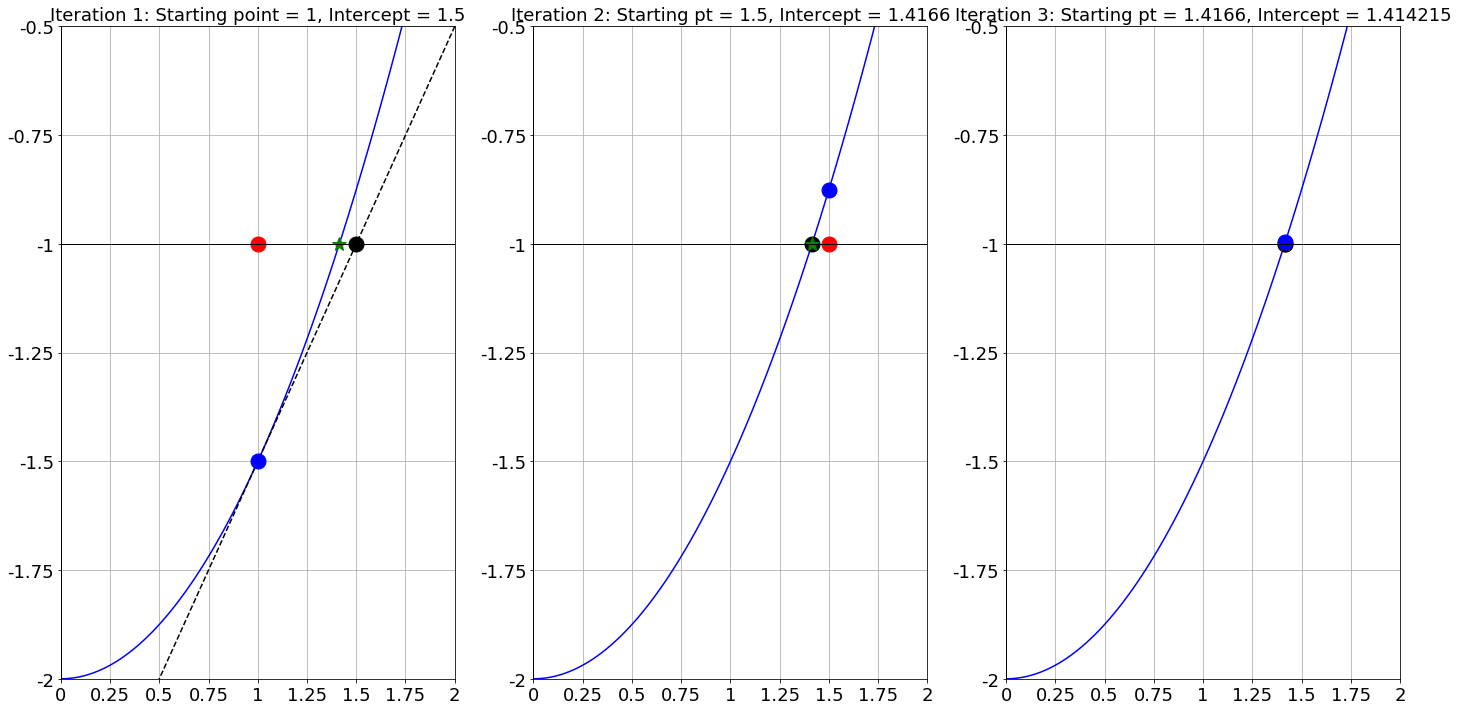
\includegraphics[width=0.75\linewidth]{images/Ch02Sec04_Newton01} 

}

\caption{Using successive tangent line approximations to find the root of a function}\label{fig:newton01}
\end{figure}

\begin{center}\rule{0.5\linewidth}{0.5pt}\end{center}

\begin{exercise}
\protect\hypertarget{exr:unnamed-chunk-101}{}{\label{exr:unnamed-chunk-101} }If we had started at \(x=0\) in the previous problem what would have
happened? Would this initial guess have worked to eventually approximate
the root?
\end{exercise}

\begin{center}\rule{0.5\linewidth}{0.5pt}\end{center}

\begin{exercise}
\protect\hypertarget{exr:unnamed-chunk-102}{}{\label{exr:unnamed-chunk-102} }Make a complete list of what you must know about the function \(f(x)\) for
the previous algorithm to work?
\end{exercise}

\begin{center}\rule{0.5\linewidth}{0.5pt}\end{center}

The algorithm that we just played with is known as Newton's Method. The
method was originally proposed by Isaac Newton, and later modified by
Joseph Raphson, for approximating roots of the algebraic equation \(f(x)=0\). It should
be clear that Newton's method requires the existence of the first
derivative so we are asking a bit more of our functions than we were
before. In Bisection and Regula Falsi we only asked that the functions
be continuous, now we're asking that they be differentiable. Stop and think for a moment \ldots{} why is this a more restrictive thing to ask for of the function \(f(x)\)?

\begin{center}\rule{0.5\linewidth}{0.5pt}\end{center}

\begin{exercise}[Newton's Method]
\protect\hypertarget{exr:newtons-method}{}{\label{exr:newtons-method} \iffalse (Newton's Method) \fi{} }The Newton-Raphson method for solving algebraic equations can be
described as follows:

\begin{enumerate}
\def\labelenumi{\arabic{enumi}.}
\item
  Check that \(f\) is differentiable on a given domain and find a way to
  guarantee that \(f\) has a root on that domain (this step happens by
  hand, not on the computer).
\item
  Pick a starting point \(x_0\) in the domain
\item
  We want to write the equation of a tangent line to \(f\) at the point
  \((x_0,  f(x_0))\).

  \begin{enumerate}
  \def\labelenumii{\roman{enumii}.}
  \item
    What is the slope of the tangent line to the function \(f(x)\) at
    the point \((x_0, f(x_0))\)?
    \[m_{tangent} = \underline{\hspace{0.5in}}\]
  \item
    Using the point-slope form of a line, \(y-y_1 = m(x-x_1)\), write
    the equation of the tangent line to \(f(x)\) at the point
    \((x_0, f(x_0))\).
    \[y - \underline{\hspace{0.4in}} = \underline{\hspace{0.4in}} \cdot \left(
                  x - \underline{\hspace{0.4in}} \right)\]
  \end{enumerate}
\item
  Find the \(x\) intercept of the equation of the tangent line by
  setting \(y=0\) and solving for \(x\). Call this new point \(x_1\).
  \[x_1 = \underline{\hspace{2in}}\]
\item
  Now iterate the process by replacing the labels ``\(x_1\)'' and ``\(x_0\)''
  in the previous step with \(x_{n+1}\) and \(x_{n}\) respectively.
  \[x_{n+1} = \underline{\hspace{2in}}\]
\item
  Iterate step 5 until \(f(x_{n})\) is \emph{close} to zero.
\end{enumerate}
\end{exercise}

\begin{center}\rule{0.5\linewidth}{0.5pt}\end{center}

\begin{exercise}
\protect\hypertarget{exr:unnamed-chunk-103}{}{\label{exr:unnamed-chunk-103} }Draw a picture of what Newton's method does graphically.
\end{exercise}

\begin{center}\rule{0.5\linewidth}{0.5pt}\end{center}

\begin{exercise}
\protect\hypertarget{exr:unnamed-chunk-104}{}{\label{exr:unnamed-chunk-104} }Create a new Python function called and write comments giving pseudo-code for
Newton's method. This version of Newton's method will accept the
function and the first derivative so you don't need to set aside any
code for calculating the derivative.
\end{exercise}

\begin{center}\rule{0.5\linewidth}{0.5pt}\end{center}

\begin{exercise}
\protect\hypertarget{exr:unnamed-chunk-105}{}{\label{exr:unnamed-chunk-105} }Write a Python function for Newton's method. Your function needs to accept a Python function for \(f(x)\), a Python function for \(f'(x)\), an initial guess,
and an optional error tolerance. The only output should be the solution
to the equation that you are solving. Write a test script to verify that
your Newton's method code indeed works.
\end{exercise}

\begin{center}\rule{0.5\linewidth}{0.5pt}\end{center}

\hypertarget{analysis-2}{%
\subsection{Analysis}\label{analysis-2}}

There are several ways in which Newton's Method will behave unexpectedly
-- or downright fail. Some of these issues can be foreseen by examining
the Newton iteration formula
\[ x_{n+1} = x_n - \frac{f(x_n)}{f'(x_n)}. \]
Some of the failures that we'll see are a little more surprising. Also in this section we will look at the convergence rate of Newton's Method and we will show that we can greatly outperform the Bisection and Regula-Falsi methods.

\begin{center}\rule{0.5\linewidth}{0.5pt}\end{center}

\begin{exercise}
\protect\hypertarget{exr:unnamed-chunk-106}{}{\label{exr:unnamed-chunk-106} }There are several reasons why Newton's method could fail. Work with your
partners to come up with a list of reasons. Support each of
your reasons with a sketch or an algebraic example.
\end{exercise}

\begin{center}\rule{0.5\linewidth}{0.5pt}\end{center}

\begin{exercise}
\protect\hypertarget{exr:unnamed-chunk-107}{}{\label{exr:unnamed-chunk-107} }One of the failures of Newton's Method is that it requires a division by \(f'(x_n)\). If \(f'(x_n)\) is zero then the algorithm completely fails. Go back to your Python function and put an \texttt{if} statement in the function that catches instances when Newton's Method fails in this way.
\end{exercise}

\begin{center}\rule{0.5\linewidth}{0.5pt}\end{center}

\begin{exercise}
\protect\hypertarget{exr:unnamed-chunk-108}{}{\label{exr:unnamed-chunk-108} }An interesting failure can occur with Newton's Method that you might not
initially expect. Consider the function \(f(x) = x^3 - 2x + 2\). This
function has a root near \(x=-1.77\). Fill in the table below and draw the
tangent lines on the figure for approximating the solution to \(f(x) = 0\)
with a starting point of \(x=0\).

\begin{longtable}[]{@{}lll@{}}
\toprule
\(n\) & \(x_n\) & \(f(x_n)\)\tabularnewline
\midrule
\endhead
\(0\) & \(x_0 = 0\) & \(f(x_0) = 2\)\tabularnewline
\(1\) & \(x_1 = 0 - \frac{f(x_0)}{f'(x_0)} = 1\) & \(f(x_1) = 1\)\tabularnewline
\(2\) & \(x_2 = 1 - \frac{f(x_1)}{f'(x_1)} =\) & \(f(x_2) =\)\tabularnewline
\(3\) & \(x_3 =\) & \(f(x_3) =\)\tabularnewline
\(4\) & \(x_4 =\) & \(f(x_4) =\)\tabularnewline
\(\vdots\) & \(\vdots\) & \(\vdots\)\tabularnewline
\bottomrule
\end{longtable}
\end{exercise}

\begin{figure}

{\centering 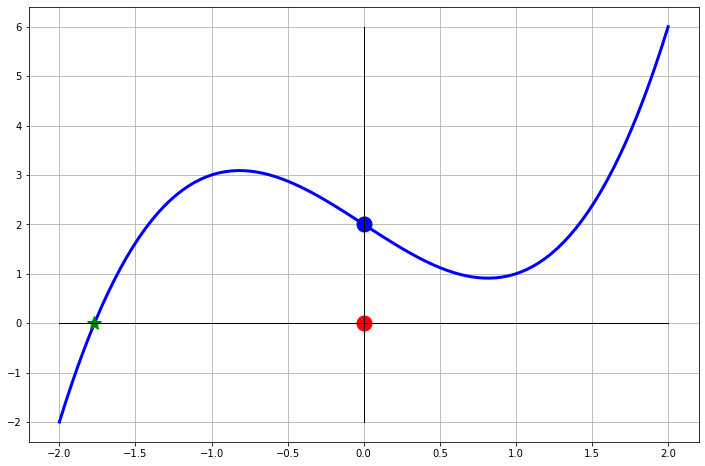
\includegraphics[width=0.5\linewidth]{images/Ch02Sec04_Newton02} 

}

\caption{An interesting Newton's Method failure.}\label{fig:newton02}
\end{figure}

\begin{center}\rule{0.5\linewidth}{0.5pt}\end{center}

\begin{exercise}
\protect\hypertarget{exr:unnamed-chunk-109}{}{\label{exr:unnamed-chunk-109} }Now let's consider the function \(f(x) = \sqrt[3]{x}\). This function has
a root \(x=0\). Furthermore, it is differentiable everywhere except at
\(x=0\) since \[f'(x) = \frac{1}{3} x^{-2/3} = \frac{1}{3x^{2/3}}.\] The
point of this problem is to show what can happen when the point of
non-differentiability is precisely the point that you're looking for.

\begin{enumerate}
\def\labelenumi{\alph{enumi}.}
\tightlist
\item
  Fill in the table of iterations starting at \(x=-1\), draw the tangent
  lines on the plot, and make a general observation of what is
  happening with the Newton iterations.
\end{enumerate}

\begin{longtable}[]{@{}lll@{}}
\toprule
\(n\) & \(x_n\) & \(f(x_n)\)\tabularnewline
\midrule
\endhead
\(0\) & \(x_0 = -1\) & \(f(x_0) = -1\)\tabularnewline
\(1\) & \(x_1 = -1 - \frac{f(-1)}{f'(-1)} =\) & \(f(x_1) =\)\tabularnewline
\(2\) & &\tabularnewline
\(3\) & &\tabularnewline
\(4\) & &\tabularnewline
\(\vdots\) & \(\vdots\) & \(\vdots\)\tabularnewline
\bottomrule
\end{longtable}
\end{exercise}

\begin{figure}

{\centering 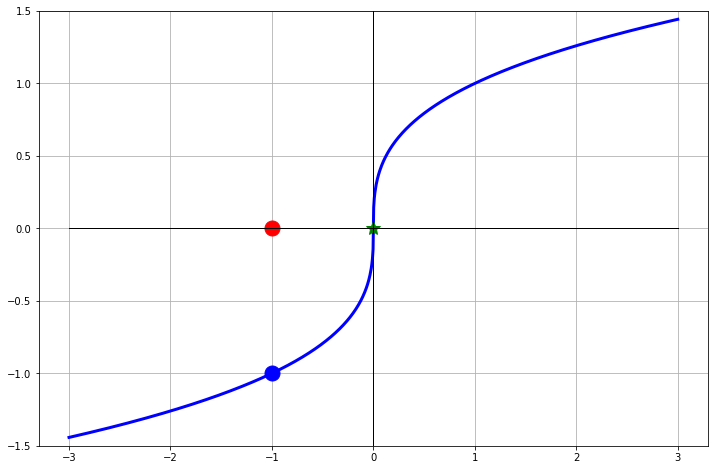
\includegraphics[width=0.5\linewidth]{images/Ch02Sec04_Newton03} 

}

\caption{Another surprising Newton's Method failure.}\label{fig:newton03}
\end{figure}

\begin{enumerate}
\def\labelenumi{\alph{enumi}.}
\setcounter{enumi}{1}
\item
  Now let's look at the Newton iteration in a bit more detail. Since
  \(f(x) = x^{1/3}\) and \(f'(x) = \frac{1}{3} x^{-2/3}\) the Newton iteration
  can be simplified as
  \[x_{n+1} = x_n - \frac{x^{1/3}}{ \left( \frac{1}{3} x^{-2/3} \right)} = x_n - 3 \frac{x^{1/3}}{x^{-2/3}} =
      x_n - 3x_n = -2x_n.\] What does this tell us about the Newton
  iterations?\\
  Hint: You should have found the exact same thing in the numerical
  experiment in part (a).
\item
  Was there anything special about the starting point \(x_0=-1\)? Will
  this problem exist for every starting point?
\end{enumerate}

\begin{center}\rule{0.5\linewidth}{0.5pt}\end{center}

\begin{exercise}
\protect\hypertarget{exr:unnamed-chunk-110}{}{\label{exr:unnamed-chunk-110} }Repeat the previous exercise with the function \(f(x) = x^3 - 5x\) with the starting point \(x_0 = -1\).
\end{exercise}

\begin{figure}

{\centering 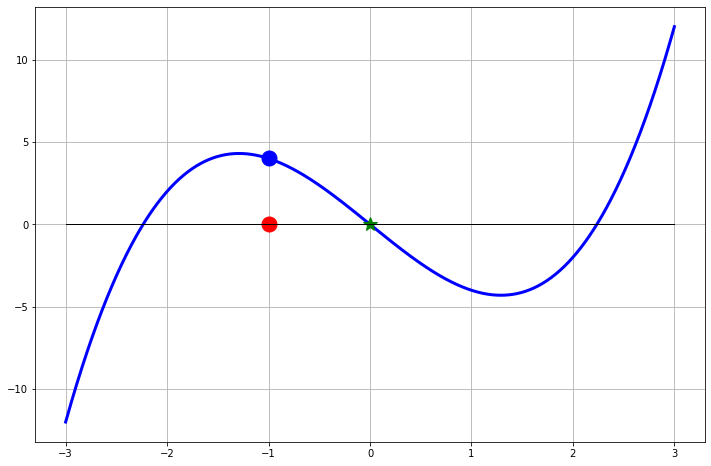
\includegraphics[width=0.5\linewidth]{images/Ch02Sec04_Newton04} 

}

\caption{Another surprising Newton's Method failure.}\label{fig:newton04}
\end{figure}

\begin{center}\rule{0.5\linewidth}{0.5pt}\end{center}

\begin{exercise}
\protect\hypertarget{exr:unnamed-chunk-111}{}{\label{exr:unnamed-chunk-111} }Newton's Method is known to have a
\emph{quadratic convergence rate}. This means that there is some constant \(C\)
such that \[|x_{k+1} - x_*| \leq C |x_{k} - x_*|^2,\] where \(x_*\) is the
root that we're hunting for.

The quadratic convergence implies that if we plot the error in the new iterate on the \(y\)-axis and
the error in the old iterate on the \(x\) axis of a log-log plot then we
will see a constant slope of 2. To see this we can take the log (base
10) of both sides of the previous equation to get
\[\log(|x_{k+1} - x_*|) = \log(C) + 2 \log(|x_{k} - x_*|),\]
and we see that this is a linear function (on a log-log plot) and the slope is 2. We created plots like this back in Example \ref{exm:bisectionplots}.

We are going to create an error plot just like what we just described.

\begin{enumerate}
\def\labelenumi{\alph{enumi}.}
\tightlist
\item
  Pick an algebraic equation where you know the solution.\\
\item
  Create the error plot with \(|x_{k} - x_*|\) on the horizontal axis and \(|x_{k+1} - x_*|\) on the vertical axis
\item
  Demonstrate that this plot has a slope of 2.
\item
  Give a thorough explanation for how to interpret the plot that you just made.
\end{enumerate}
\end{exercise}

\begin{center}\rule{0.5\linewidth}{0.5pt}\end{center}

\hypertarget{the-secant-method}{%
\section{The Secant Method}\label{the-secant-method}}

\hypertarget{intuition-and-implementation-3}{%
\subsection{Intuition and Implementation}\label{intuition-and-implementation-3}}

Newton's Method has second-order (quadratic) convergence and, as such, will perform faster than the Bisection and Regula-Falsi methods. However, Newton's Method requires that you have a function and a derivative of that function. The conundrum here is that sometimes the derivative is cumbersome or impossible to obtain but you still want to have the great quadratic convergence exhibited by Newton's method.

Recall that Newton's method is
\[x_{n+1} = x_n - \frac{f(x_n)}{f'(x_n)}.\] If we replace \(f'(x_n)\) with
an approximation of the derivative then we may have a method that is
\emph{close} to Newton's method in terms of convergence rate but is less
troublesome to compute. Any method that replaces the derivative in
Newton's method with an approximation is called a \textbf{Quasi-Newton
Method}. The first, and most obvious, way to approximate the derivative is just to
use the slope of a secant line instead of the slope a tangent line in the Newton iteration. If
we choose two starting points that are quite close to each other then
the slope of the secant line through those points will be approximately
the same as the slope of the tangent line.

\begin{center}\rule{0.5\linewidth}{0.5pt}\end{center}

\begin{exercise}[The Secant Method]
\protect\hypertarget{exr:secant-method}{}{\label{exr:secant-method} \iffalse (The Secant Method) \fi{} }Assume that \(f(x)\) is continuous and we wish to solve \(f(x) = 0\) for
\(x\).

\begin{enumerate}
\def\labelenumi{\arabic{enumi}.}
\item
  Determine if there is a root \emph{near} an arbitrary starting point
  \(x_0\). How might you do that?
\item
  Pick a second starting point \emph{near} \(x_0\). Call this second starting
  point \(x_1\). Note well that the points \(x_0\) and \(x_1\) should be
  close to each other. Why?\\
  (The choice here is different than for the Bisection and Regula
  Falsi methods. We are \emph{not} choosing the left- and right- sides of an interval surrounding the root.)
\item
  Use the backward difference
  \[f'(x_n) \approx \frac{f(x_n) - f(x_{n-1})}{x_n - x_{n-1}}\] to
  approximate the derivative of \(f\) at \(x_n\). ~Discuss why this approximates the derivative.
\item
  Perform the Newton-type iteration
  \[x_{n+1} = x_n - \frac{f(x_n)}{ \left(  \frac{f(x_n) - f(x_{n-1})}{x_n - x_{n-1}}\right)}\]
  until \(f(x_n)\) is \emph{close enough} to zero. Notice that the new
  iteration simplifies to
  \[x_{n+1} = x_n - \frac{f(x_n)\left( x_n - x_{n-1} \right)}{f(x_n) -
              f(x_{n-1})}.\]
\end{enumerate}
\end{exercise}

\begin{center}\rule{0.5\linewidth}{0.5pt}\end{center}

\begin{exercise}
\protect\hypertarget{exr:unnamed-chunk-112}{}{\label{exr:unnamed-chunk-112} }Draw several pictures showing what the Secant method does pictorially.
\end{exercise}

\begin{center}\rule{0.5\linewidth}{0.5pt}\end{center}

\begin{exercise}
\protect\hypertarget{exr:unnamed-chunk-113}{}{\label{exr:unnamed-chunk-113} }Write pseudo-code to outline how you will implement the Secant Method.
\end{exercise}

\begin{center}\rule{0.5\linewidth}{0.5pt}\end{center}

\begin{exercise}
\protect\hypertarget{exr:unnamed-chunk-114}{}{\label{exr:unnamed-chunk-114} }Write Python code for solving algebraic equations of the form \(f(x) = 0\) with
the Secant method. Your function should accept a Python function, two starting points, and an optional error tolerance. Also write a test script that clearly shows that your
code is working.
\end{exercise}

\begin{center}\rule{0.5\linewidth}{0.5pt}\end{center}

\hypertarget{analysis-3}{%
\subsection{Analysis}\label{analysis-3}}

Up to this point we have done analysis work on the Bisection Method, the Regula-Falsi Method, and Newton's Method. We have found that the methods are first order, first order, and second order respectively. We end this chapter by doing the same for the Secant Method.

\begin{center}\rule{0.5\linewidth}{0.5pt}\end{center}

\begin{exercise}
\protect\hypertarget{exr:unnamed-chunk-115}{}{\label{exr:unnamed-chunk-115} }Choose a non-trivial algebraic equation for which you know the solution
and write a script to empirically determine the convergence rate of the
Secant method.
\end{exercise}

\begin{center}\rule{0.5\linewidth}{0.5pt}\end{center}

\hypertarget{exercises-1}{%
\section{Exercises}\label{exercises-1}}

\hypertarget{algorithm-summaries}{%
\subsection{Algorithm Summaries}\label{algorithm-summaries}}

The following four problems are meant to have you re-build each of the
algorithms that we developed in this chapter. Write all of the
mathematical details completely and clearly. Don't just write ``how'' the
method works, but give all of the mathematical details for ``why'' it
works.

\begin{center}\rule{0.5\linewidth}{0.5pt}\end{center}

\begin{exercise}
\protect\hypertarget{exr:unnamed-chunk-116}{}{\label{exr:unnamed-chunk-116} }Let \(f(x)\) be a continuous function on the interval \([a,b]\) where
\(f(a) \cdot f(b) < 0\). Clearly give all of the mathematical details for how the
Bisection Method approximates the root of the function \(f(x)\) in the
interval \([a,b]\).
\end{exercise}

\begin{center}\rule{0.5\linewidth}{0.5pt}\end{center}

\begin{exercise}
\protect\hypertarget{exr:unnamed-chunk-117}{}{\label{exr:unnamed-chunk-117} }Let \(f(x)\) be a continuous function on the interval \([a,b]\) where
\(f(a) \cdot f(b) <  0\). Clearly give all of the mathematical details for how the Regula
Falsi Method approximates the root of the function \(f(x)\) in the
interval \([a,b]\).
\end{exercise}

\begin{center}\rule{0.5\linewidth}{0.5pt}\end{center}

\begin{exercise}
\protect\hypertarget{exr:unnamed-chunk-118}{}{\label{exr:unnamed-chunk-118} }Let \(f(x)\) be a differentiable function with a root \emph{near} \(x=x_0\).
Clearly give all of the mathematical details for how Newton's Method
approximates the root of the function \(f(x)\).
\end{exercise}

\begin{center}\rule{0.5\linewidth}{0.5pt}\end{center}

\begin{exercise}
\protect\hypertarget{exr:unnamed-chunk-119}{}{\label{exr:unnamed-chunk-119} }Let \(f(x)\) be a continuous function with a root \emph{near} \(x=x_0\). Clearly
give all of the mathematical details for how the Secant Method
approximates the root of the function \(f(x)\).
\end{exercise}

\begin{center}\rule{0.5\linewidth}{0.5pt}\end{center}

\hypertarget{applying-what-youve-learned-1}{%
\subsection{Applying What You've Learned}\label{applying-what-youve-learned-1}}

\begin{center}\rule{0.5\linewidth}{0.5pt}\end{center}

\begin{exercise}
\protect\hypertarget{exr:unnamed-chunk-120}{}{\label{exr:unnamed-chunk-120} }How many iterations of the bisection method are necessary to approximate
\(\sqrt{3}\) to within \(10^{-3}\), \(10^{-4}\), \ldots, \(10^{-15}\) using the
initial interval \([a,b]=[0,2]\)?
\end{exercise}

\begin{center}\rule{0.5\linewidth}{0.5pt}\end{center}

\begin{exercise}
\protect\hypertarget{exr:unnamed-chunk-121}{}{\label{exr:unnamed-chunk-121} }Refer back to Example \ref{exm:bisectionplots} and demonstrate that you get the same results by solving the problem \(x^3 - 3 = 0\). Generate versions of all of the plots from the Example and give thorough descriptions of what you learn from each plot.
\end{exercise}

\begin{center}\rule{0.5\linewidth}{0.5pt}\end{center}

\begin{exercise}
\protect\hypertarget{exr:unnamed-chunk-122}{}{\label{exr:unnamed-chunk-122} }In this problem you will demonstrate that all of your root finding codes
work. At the beginning of this chapter we proposed the algebraic
equation solving problem \[3\sin(x) + 9 = x^2 - \cos(x).\] Write a
script that calls upon your Bisection, Regula Falsi, Newton, and Secant
methods one at a time to find the positive solution to this equation.
Your script needs to output the solutions in a clear and readable way so
you can tell which answer can from which root finding algorithm.
\end{exercise}

\begin{center}\rule{0.5\linewidth}{0.5pt}\end{center}

\begin{exercise}
\protect\hypertarget{exr:unnamed-chunk-123}{}{\label{exr:unnamed-chunk-123} }A root-finding method has a convergence rate of order \(M\) if there is a
constant \(C\) such that \[|x_{k+1} - x_*| \leq C |x_k - x_*|^M.\] Here,
\(x_*\) is the exact root, \(x_k\) is the \(k^{th}\) iteration of the root
finding technique, and \(x_{k+1}\) is the \((k+1)^{st}\) iteration of the
root finding technique.

\begin{enumerate}
\def\labelenumi{\alph{enumi}.}
\item
  If we consider the equation \[|x_{k+1} - x_*| \leq C |x_k - x_*|^M\]
  and take the logarithm (base 10) of both sides then we get
  \[\log\left( |x_{k+1} - x_*| \right) \leq \underline{\hspace{1in}} +
              \underline{\hspace{1in}}\]
\item
  In part (a) you should have found that the log of new error is a
  linear function of the log of the old error. What is the slope of
  this linear function on a log-log plot?
\item
  In the plots below you will see three different log-log plots of the
  new error to the old error for different root finding techniques.
  What is the order of the convergence rate for each of these methods?
\end{enumerate}
\end{exercise}

\begin{figure}

{\centering \includegraphics[width=0.95\linewidth]{images/Ch02_ErrorsExercise} 

}

\caption{Three Error Plots}\label{fig:thee-error-plots}
\end{figure}

\begin{enumerate}
\def\labelenumi{\alph{enumi}.}
\setcounter{enumi}{3}
\tightlist
\item
  In your own words, what does it mean for a root finding method to
  have a ``first order convergence rate''? ``Second order convergence
  rate''? etc.
\end{enumerate}

\begin{center}\rule{0.5\linewidth}{0.5pt}\end{center}

\begin{exercise}
\protect\hypertarget{exr:unnamed-chunk-124}{}{\label{exr:unnamed-chunk-124} }Multiple Choice: For every step of Newton's method the new estimate of
the error between the Newton iteration and the exact answer is
approximately:

\begin{enumerate}
\def\labelenumi{\alph{enumi}.}
\item
  the same as it was on the previous step.
\item
  ten times smaller than it was on the previous step
\item
  one hundred times smaller than it was on the previous step
\item
  one thousand times smaller than it was on the previous step
\end{enumerate}

Defend your answer with a sentence or two.
\end{exercise}

\begin{center}\rule{0.5\linewidth}{0.5pt}\end{center}

\begin{exercise}
\protect\hypertarget{exr:unnamed-chunk-125}{}{\label{exr:unnamed-chunk-125} }There are MANY other root finding techniques beyond the four that we have studied thus far. In this problem you will built the Chebyshev Method -- named for the famous mathematician \href{https://en.wikipedia.org/wiki/Pafnuty_Chebyshev}{Pafnuty Chebyshev}.

The iteration scheme for Chebyshev's Method is given as
\[x_{n+1} = x_n - \frac{f(x_n)}{f'(x_n)} - \frac{1}{2} \left( \frac{f(x_n)}{f'(x_n)}
    \right)^2 \frac{f''(x_n)}{f'(x_n)},\]

\begin{enumerate}
\def\labelenumi{\alph{enumi}.}
\tightlist
\item
  Write a Python function that implements the Chebyshev Method.
\item
  Demonstrate that your code is indeed working by solving several problems where you know the exact solution.
\item
  Show several plots that demonstrates that the Chebyshev Method exhibits a third-order
  convergence rate. That is, create a log-log plot of the successive errors for several different equation-solving problems. What does this ``third order convergence'' mean about the successive approximations in the Chebyshev iterations?
\item
  What are the pro's and con's to using Chebyshev's method instead of Newton's method?
\end{enumerate}
\end{exercise}

\begin{center}\rule{0.5\linewidth}{0.5pt}\end{center}

\begin{exercise}
\protect\hypertarget{exr:unnamed-chunk-126}{}{\label{exr:unnamed-chunk-126} }(modified from {[}\protect\hyperlink{ref-burden}{5}{]}) An object falling vertically through the air is subject to friction due
to air resistance as well as gravity. The function describing the
position of such a function is
\[s(t) = s_0 - \frac{mg}{k} t + \frac{m^2 g}{k^2}\left( 1- e^{-kt/m} \right),\]
where \(m\) is the mass measured in kg, \(g\) is gravity measured in meters
per second per second, \(s_0\) is the initial position measured in meters,
and \(k\) is the coefficient of air resistance.

\begin{enumerate}
\def\labelenumi{\alph{enumi}.}
\item
  What are the units of the parameter \(k\)?
\item
  If \(m = 1\)kg, \(g=9.8\)m/s\(^2\), \(k=0.1\), and \(s_0 = 100\)m how long
  will it take for the object to hit the ground? Find your answer to
  within 0.01 seconds.
\item
  The value of \(k\) depends on the aerodynamics of the object and might
  be challenging to measure. We want to perform a sensitivity analysis
  on your answer to part (b) subject to small measurement errors in
  \(k\). If the value of \(k\) is only known to within 10\% then what are
  your estimates of when the object will hit the ground?
\end{enumerate}
\end{exercise}

\begin{center}\rule{0.5\linewidth}{0.5pt}\end{center}

\begin{exercise}
\protect\hypertarget{exr:unnamed-chunk-127}{}{\label{exr:unnamed-chunk-127} }Can the Bisection Method, Regula Falsi Method, or Newton's Method be used to find the roots of the function \(f(x) = cos(x) + 1\)? Explain why or why not for each technique?
\end{exercise}

\begin{center}\rule{0.5\linewidth}{0.5pt}\end{center}

\begin{exercise}
\protect\hypertarget{exr:unnamed-chunk-128}{}{\label{exr:unnamed-chunk-128} }Consider our four primary root finding methods: Bisection, Regula Falsi,
Newton's method, and the Secant method.

\begin{enumerate}
\def\labelenumi{\alph{enumi}.}
\item
  For each method give a mathematical situation where you might want
  to use the method and give a mathematical situation where you might
  not want to use the method.
\item
  For each of these methods give one example where the method will
  fail.
\end{enumerate}

Support your arguments with proper mathematics. You are welcome to argue
graphically but be sure to fully explain your graphical reasoning.
\end{exercise}

\begin{center}\rule{0.5\linewidth}{0.5pt}\end{center}

\begin{exercise}
\protect\hypertarget{exr:unnamed-chunk-129}{}{\label{exr:unnamed-chunk-129} }In Single Variable Calculus you studied methods for finding local and
global extrema of functions. You likely recall that part of the process
is to set the first derivative to zero and to solve for the independent
variable (remind yourself why you're doing this). The trouble with this
process is that it may be very very challenging to do the algebraic
solve by hand. This is a perfect place for Newton's method or any other
root finding techinque!\\
Find the local extrema for the function \(f(x) = x^3(x-3)(x-6)^4\) using numerical techniques where appropriate.
\end{exercise}

\begin{center}\rule{0.5\linewidth}{0.5pt}\end{center}

\begin{exercise}
\protect\hypertarget{exr:unnamed-chunk-130}{}{\label{exr:unnamed-chunk-130} }A \emph{fixed point} of a function \(f(x)\) is a point that solves the equation
\(f(x) =  x\). Fixed points are interesting in iterative processes since fixed
points don't change under repeated application of the function \(f\).

For example, consider the function \(f(x) = x^2 - 6\). The fixed points of
\(f(x)\) can be found by solving the equation \(x^2 - 6 = x\) which, when
simplified algebraically, is \(x^2 - x -  6 = 0\). Factoring the left-hand side gives \((x-3)(x+2)=0\) which
implies that \(x=3\) and \(x=-2\) are fixed points for this function. That
is, \(f(3) = 3\) and \(f(-2) = -2\). Notice, however, that finding fixed
points is identical to a root finding problem.

\begin{enumerate}
\def\labelenumi{\alph{enumi}.}
\item
  Use a numerical root-finding algorithm to find the fixed points of
  the function \(f(x) = x^2 - 6\) on the interval \([0,\infty)\).
\item
  Find the fixed points of the function \(f(x) =  \sqrt{\frac{8}{x+6}}\).
\end{enumerate}
\end{exercise}

\begin{center}\rule{0.5\linewidth}{0.5pt}\end{center}

\begin{exercise}[`scipy.optimize.fsolve()`]
\protect\hypertarget{exr:fsolve}{}{\label{exr:fsolve} \iffalse (\texttt{scipy.optimize.fsolve()}) \fi{} }The \texttt{scipy} library in Python has many built-in numerical analysis routines much like the ones that we have built in this chapter. Of particular interest to the task of algebraic root finding is the \texttt{fsolve} command in the \texttt{scipy.optimize} library.

\begin{enumerate}
\def\labelenumi{\alph{enumi}.}
\tightlist
\item
  Go to the \href{https://docs.scipy.org/doc/scipy/reference/generated/scipy.optimize.fsolve.html}{help documentation} for \texttt{scipy.optimize.fsolve} and make yourself familiar with how to use the tool.
\item
  First solve the algebraic equation \(x\sin(x) - \ln(x) = 0\) for \(x\) starting at \(x_0 = 3\).

  \begin{enumerate}
  \def\labelenumii{\roman{enumii}.}
  \tightlist
  \item
    Make a plot of the function on the domain \([0,5]\) so you can eyeball the root before using the tool.
  \item
    Use the \texttt{scipy.optimize.fsolve()} command to approximate the root.
  \item
    Fully explain each of the outputs from the \texttt{scipy.optimize.fsolve()} command. You should use the \texttt{fsolve()} command with \texttt{full\_output=1} so you can see all of the solver diagnostics.
  \end{enumerate}
\item
  Demonstrate how to use \texttt{fsolve()} using any non-trivial nonlinear algebraic equation solving problem. Demonstrate what some of the options of \texttt{fsolve()} do.
\item
  The \texttt{scipy.optimize.fsolve()} command can also solve systems of equations (something we have not built algorithms for in this chapter). Consider the system of equations
  \[ \begin{aligned} x_0 \cos(x_1) &= 4 \\ x_0 x_1 - x_1 &= 5  \end{aligned} \]
  The following Python code allows you to use \texttt{scipy.optimize.fsolve()} so solve this system of nonlinear equations in much the same way as we did in part (b) of this problem. However, be aware that we need to think of \texttt{x} as a vector of \(x\)-values. Go through the code below and be sure that you understand every line of code.
\item
  Solve the system of nonlinear algebraic equation below using \texttt{scipy.optimize.fsolve()}.
  \[ \begin{aligned} x^2-xy^2 &=2 \\ xy &= 2 \end{aligned} \]
\end{enumerate}
\end{exercise}

\begin{Shaded}
\begin{Highlighting}[]
\ImportTok{import}\NormalTok{ numpy }\ImportTok{as}\NormalTok{ np}
\ImportTok{from}\NormalTok{ scipy.optimize }\ImportTok{import}\NormalTok{ fsolve}

\KeywordTok{def}\NormalTok{ F(x):}
\NormalTok{  Output }\OperatorTok{=}\NormalTok{ [x[}\DecValTok{0}\NormalTok{]}\OperatorTok{*}\NormalTok{np.cos(x[}\DecValTok{1}\NormalTok{])}\OperatorTok{{-}}\DecValTok{4}\NormalTok{]}
\NormalTok{  Output.append( x[}\DecValTok{0}\NormalTok{]}\OperatorTok{*}\NormalTok{x[}\DecValTok{1}\NormalTok{] }\OperatorTok{{-}}\NormalTok{ x[}\DecValTok{1}\NormalTok{] }\OperatorTok{{-}} \DecValTok{5}\NormalTok{ )}
  \ControlFlowTok{return}\NormalTok{ Output}

\NormalTok{fsolve(F,[}\DecValTok{6}\NormalTok{,}\DecValTok{1}\NormalTok{],full\_output}\OperatorTok{=}\DecValTok{1}\NormalTok{) }\CommentTok{\# Note: full\_output gives the solver diagnostics}
\end{Highlighting}
\end{Shaded}

\begin{center}\rule{0.5\linewidth}{0.5pt}\end{center}

\hypertarget{projects}{%
\section{Projects}\label{projects}}

At the end of every chapter we propose a few projects related to the content in the preceding chapter(s). In this section we propose one ideas for a project related to numerical algebra. The projects in this book are meant to be open ended, to encourage creative mathematics, to push your coding skills, and to require you to write and communicate your mathematics. Take the time to read Appendix \ref{ch:writing} before you write your final paper.

\hypertarget{basins-of-attraction}{%
\subsection{Basins of Attraction}\label{basins-of-attraction}}

Let \(f(x)\) be a differentiable function with several roots. Given a
starting \(x\) value we should be able to apply Newton's Method to that
starting point and we will converge to one of the roots (so long as you
aren't in one of the special cases discussed earlier in the chapter). It
stands to reason that starting points \emph{near} each other should all end
up at the same root, and for some functions this is true. However, it is
not true in general.

A \textbf{basin of attraction} for a root is the set of \(x\) values that
converges to that root under Newton iterations. In this problem you will
produce colored plots showing the basins of attraction for all of the
following functions. Do this as follows:

\begin{itemize}
\item
  Find the actual roots of the function by hand (this should be easy
  on the functions below).
\item
  Assign each of the roots a different color.
\item
  Pick a starting point on the \(x\) axis and use it to start Newton's
  Method.
\item
  Color the starting point according to the root that it converges to.
\item
  Repeat this process for many many starting points so you get a
  colored picture of the \(x\) axis showing where the starting points
  converge to.
\end{itemize}

The set of points that are all the same color are called the \textbf{basin of
attraction} for the root associated with that color. In Figure \ldots{} there is an image of a sample basin of attraction image.

\begin{figure}

{\centering 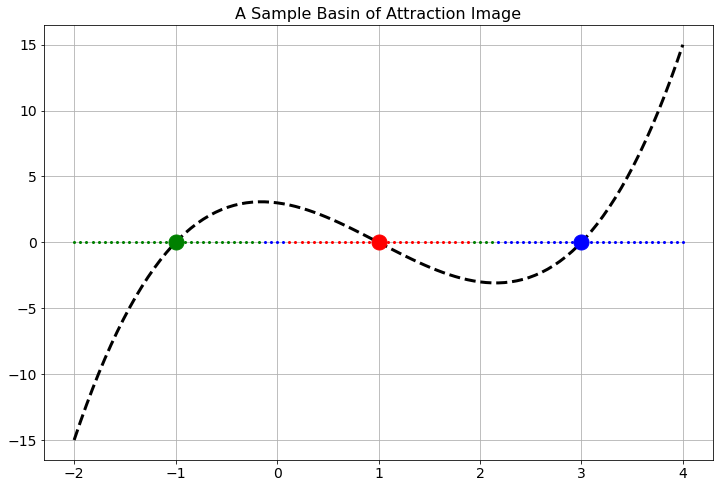
\includegraphics[width=0.6\linewidth]{images/Ch02ProjectBasin} 

}

\caption{A sample basin of attraction image for a cubic function.}\label{fig:basin}
\end{figure}

\begin{enumerate}
\def\labelenumi{\arabic{enumi}.}
\item
  Create a basin on attraction image for the function \(f(x) = (x-4)(x+1)\).
\item
  Create a basin on attraction image for the function \(g(x) = (x-1)(x+3)\).
\item
  Create a basin on attraction image for the function \(h(x) = (x-4)(x-1)(x+3)\).
\item
  Find a non-trivial single-variable function of your own that has an interesting
  picture of the basins of attraction. In your write up explain why you thought that this was an interesting function in terms of the basins of attraction.
\item
  Now for the fun part! Consider the function \(f(z) = z^3 - 1\) where
  \(z\) is a complex variable. That is, \(z = x + iy\) where
  \(i = \sqrt{-1}\). From the Fundamental Theorem of Algebra we know
  that there are three roots to this polynomial in the complex plane.
  In fact, we know that the roots are \(z_0 =  1\), \(z_1 = \frac{1}{2}\left( -1 + \sqrt{3} i \right)\), and
  \(z_2 =  \frac{1}{2} \left( -1 - \sqrt{3} i \right)\) (you should stop
  now and check that these three numbers are indeed roots of the
  polynomial \(f(z)\)). Your job is to build a picture of the basins of
  attraction for the three roots in the complex plane. This picture
  will naturally be two-dimensional since numbers in the complex plane
  are two dimensional (each has a real and an imaginary part). When
  you have your picture give a thorough write up of what you found.
\item
  Now pick your favorite complex-valued function and build a picture
  of the basins of attraction. Consider this an art project! See if
  you can come up with the prettiest basin of attraction picture.
\end{enumerate}

\hypertarget{artillery}{%
\subsection{Artillery}\label{artillery}}

An artillery officer wishes to fire his cannon on an enemy brigade. He wants to know the angle to aim the cannon in order to strike the target. If we have control over the initial velocity of the cannon ball, \(v_0\), and the angle of the cannon above horizontal, \(\theta\), then the initial vertical component of the velocity of the ball is \(v_y(0) = v_0 \sin(\theta)\) and the initial horizontal component of the velocity of the ball is \(v_x(0) = v_0 \cos(\theta)\). In this problem we will assume the following:

\begin{itemize}
\tightlist
\item
  We will neglect air resistance\footnote{Strictly speaking, neglecting air resistance is a poor assumption since a cannon ball moves fast enough that friction with the air plays a non-negligible role. However, the assumption of no air resistance greatly simplifies the math and makes this version of the problem more tractable. The second version of the artillery problem in Chapter \ref{ch:odes} will look at the effects of air resistance on the cannon ball.} so for all time differential equations \(v_y'(t) = -g\) and \(v_x'(t) = 0\) must both hold.
\item
  We will assume that the position of the cannon is the origin of a coordinate system so \(s_x(0) = 0\) and \(s_y(0) = 0\).
\item
  We will assume that the target is at position \((x_*,y_*)\) which you can measure accurately relative to the cannon's position. The landscape is relatively flat but \(y_*\) could be a bit higher or a bit lower than the cannon's position.
\end{itemize}

Use the given information to write a nonlinear equation\footnote{Hint: Symbolically work out the amount of time that it takes until the vertical position of the cannon ball reaches \(y_*\). Then substitute that time into the horizontal position, and set the horizontal position equation to \(x_*\).} that relates \(x_*\), \(y_*\), \(v_0\), \(g\), and \(\theta\). We know that \(g = 9.8m/s^2\) is constant and we will assume that the initial velocity can be adjusted between \(v_0 = 100m/s\) and \(v_0 = 150m/s\) in increments of \(10m/s\). If we then are given a fixed value of \(x_*\) and \(y_*\) the only variable left to find in your equation is \(\theta\). A numerical root-finding technique can then be applied to your equation to approximate the angle. Create several look up tables for the artillery officer so they can be given \(v_0\), \(x_*\), and \(y_*\) and then use your tables to look up the angle at which to set the cannon. Be sure to indicate when a target is out of range.

Write a brief technical report detailing your methods. Support your work with appropriate mathematics and plots. Include your tables at the end of your report.

\hypertarget{ch:calculus}{%
\chapter{Calculus}\label{ch:calculus}}

\hypertarget{intro-to-numerical-calculus}{%
\section{Intro to Numerical Calculus}\label{intro-to-numerical-calculus}}

In this chapter we build some of the common techniques for approximating
the two primary computations in calculus: taking derivatives and
evaluating definite integrals. Beyond differentiation and integration one of the major applications of differential calculus was optimization. The last several sections of this chapter focus on numerical routines for approximating the solutions to optimization problems.

Recall the typical tools of differential calculus:

\begin{itemize}
\tightlist
\item
  the power rule,
\item
  the chain rule,
\item
  the product rule,
\item
  the quotient rule,
\item
  the differentiation rules for exponentials, inverses, and trig
  functions,
\item
  implicit differentiation,
\item
  etc.
\end{itemize}

With these rules, and enough time and patience, we can find a derivative
of any algebraically defined function. The truth of the matter is that
not all functions are given to us algebraically, and even the ones that
are given algebraically are sometimes really cumbersome.

\begin{center}\rule{0.5\linewidth}{0.5pt}\end{center}

\begin{exercise}
\protect\hypertarget{exr:unnamed-chunk-132}{}{\label{exr:unnamed-chunk-132} }A water quality engineering team wants to find the rate at which the
volume of waste water is changing in their containment pond throughout
the year. They presently only have data on the specific geometric shape
of the containment pond as well as the depth of the waste water each day
for the past year. Propose several methods for approximating the first
derivative of the volume of the waste water pond.
\end{exercise}

\begin{center}\rule{0.5\linewidth}{0.5pt}\end{center}

\begin{exercise}
\protect\hypertarget{exr:unnamed-chunk-133}{}{\label{exr:unnamed-chunk-133} }When a police officer fires a radar gun at a moving car it uses a laser
to measure the distance from the officer to the car:

\begin{itemize}
\item
  The speed of light is constant.
\item
  The time between when the laser is fired and when the light
  reflected off of the car is received can be measured very
  accurately.
\item
  Using the formula \(\text{distance} = \text{rate} \cdot \text{time}\),
  the time for the laser pulse to be sent and received can then be
  converted to a distance.
\end{itemize}

How does the radar gun then use that information to calculate the speed
of the moving car?
\end{exercise}

\begin{center}\rule{0.5\linewidth}{0.5pt}\end{center}

Integration, on the other hand, is a more difficult situation. You may
recall some of the techniques of integral calculus such as the power
rule, \(u\)-substitution, and integration by parts. However, these tools
are not enough to find an antiderviative for any given function.
Furthermore, not every function can be written algebraically.

\begin{center}\rule{0.5\linewidth}{0.5pt}\end{center}

\begin{exercise}
\protect\hypertarget{exr:unnamed-chunk-134}{}{\label{exr:unnamed-chunk-134} }In statistics the function known as \emph{the normal distribution} (the bell
curve) is defined as \[N(x) = \frac{1}{\sqrt{2\pi}} e^{-x^2/2}.\] One of
the primary computations of introductory statistics is to find the area
under a portion of this curve since this area gives the probability of
some event
\[P(a < x < b) = \int_a^b \frac{1}{\sqrt{2\pi}} e^{-x^2/2} dx.\] The
trouble is that there is no known antiderivative of this function.
Propose a method for approximating this area.
\end{exercise}

\begin{center}\rule{0.5\linewidth}{0.5pt}\end{center}

\begin{exercise}
\protect\hypertarget{exr:unnamed-chunk-135}{}{\label{exr:unnamed-chunk-135} }Give a list of five functions for which an exact algebraic derivative is
relatively easy but an exact antiderivative is either very hard or maybe
impossible. Be prepared to compare with your peers.
\end{exercise}

\begin{center}\rule{0.5\linewidth}{0.5pt}\end{center}

\begin{exercise}
\protect\hypertarget{exr:unnamed-chunk-136}{}{\label{exr:unnamed-chunk-136} }A dam operator has control of the rate at which water is flowing out of
a hydroelectric dam. He has records for the approximate flow rate
through the dam over the course of a day. Propose a way for the operator
to use his data to determine the total amount of water that has passed
through the dam during that day.
\end{exercise}

\begin{center}\rule{0.5\linewidth}{0.5pt}\end{center}

What you've seen here are just a few examples of why you might need to
use numerical calculus instead of the classical routines that you
learned earlier in your mathematical career. Another typical need for
numerical derivatives and integrals arises when we approximate the
solutions to differential equations in the later chapters of this book.

Throughout this chapter we will make heavy use of Taylor's Theorem to
build approximations of derivatives and integrals. If you find yourself
still a bit shaky on Taylor's Theorem it would probably be wise to go
back to Section \ref{sec:Taylor} and do a quick review.

At the end of the chapter
we'll examine a numerical technique for solving optimization problems
without explicitly finding derivatives. Then we'll look at a common use
of numerical calculus for fitting curves to data.

\hypertarget{differentiation}{%
\section{Differentiation}\label{differentiation}}

\hypertarget{the-first-derivative}{%
\subsection{The First Derivative}\label{the-first-derivative}}

\begin{exercise}
\protect\hypertarget{exr:unnamed-chunk-137}{}{\label{exr:unnamed-chunk-137} }Recall from your first-semester Calculus class that the derivative of a
function \(f(x)\) is defined as
\[f'(x) = \lim_{\Delta x \to 0} \frac{f(x+\Delta x) - f(x)}{\Delta x}\]
A Calculus student proposes that it would just be much easier if we
dropped the limit and instead just always choose \(\Delta x\) to be some
small number, like \(0.001\) or \(10^{-6}\). Discuss the following questions:

\begin{enumerate}
\def\labelenumi{\alph{enumi}.}
\item
  When might the Calculus student's proposal actually work pretty well
  in place of calculating an actual derivative?
\item
  When might the Calculus student's proposal fail in terms of approximating the derivative?
\end{enumerate}
\end{exercise}

\begin{center}\rule{0.5\linewidth}{0.5pt}\end{center}

In this section we'll build several approximation of first and second
derivatives. The primary idea for each of these approximations is:

\begin{itemize}
\tightlist
\item
  Partition the interval \([a,b]\) into \(N\) sub intervals
\item
  Define the distance between two points in the partition as \(h\).\\
\item
  Approximate the derivative at any point \(x\) in the interval \([a,b]\) by using linear combinations of \(f(x-h)\), \(f(x)\), \(f(x+h)\), and/or other points in the partition.
\end{itemize}

Partitioning the interval into discrete points turns the continuous
problem of finding a derivative at every real point in \([a,b]\) into a
discrete problem where we calculate the approximate derivative at
finitely many points in \([a,b]\).

\begin{figure}

{\centering 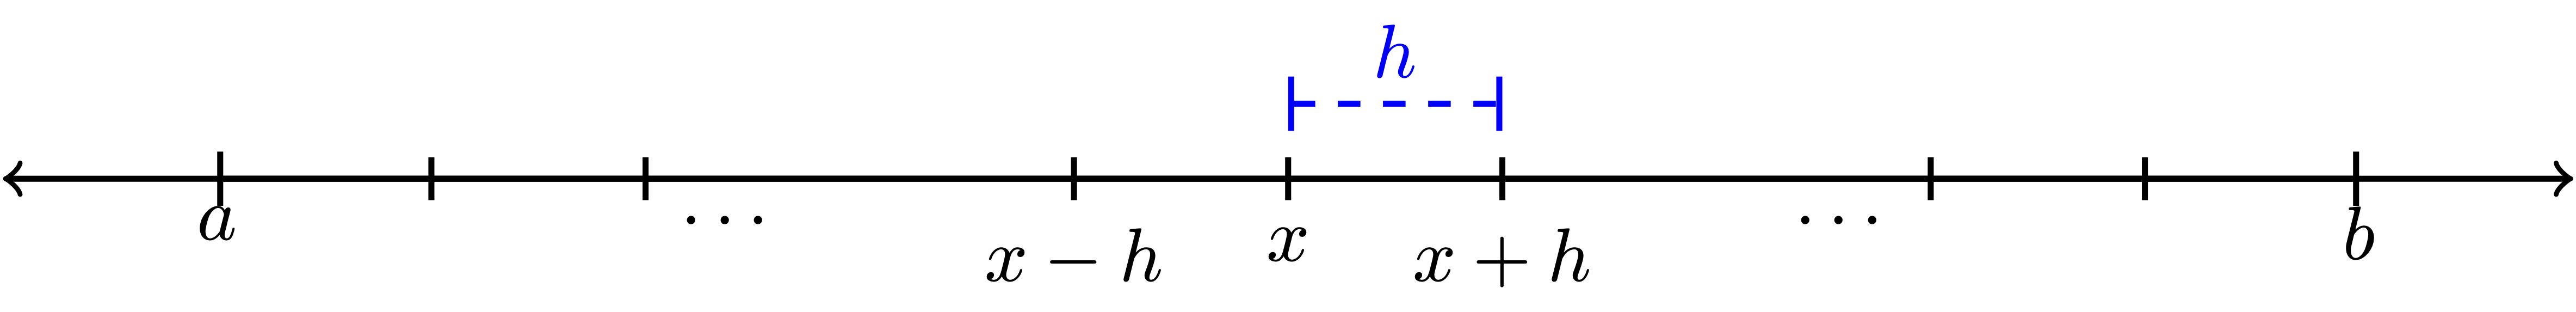
\includegraphics[width=0.75\linewidth]{images/Ch03_IntervalPartition} 

}

\caption{A partition of the interval $[a,b]$.}\label{fig:differentiation-partition}
\end{figure}

Figure \ref{fig:differentiation-partition} shows a depiction of the
partition as well as making clear that \(h\) is the separation between
each of the points in the partition. Note that in general the points in
the partition do not need to be equally spaced, but that is the simplest
place to start.

\begin{center}\rule{0.5\linewidth}{0.5pt}\end{center}

\begin{exercise}
\protect\hypertarget{exr:unnamed-chunk-138}{}{\label{exr:unnamed-chunk-138} }Let's take a close look at partitions before moving on to more details about numerical differentiation.

\begin{enumerate}
\def\labelenumi{\alph{enumi}.}
\tightlist
\item
  If we partition the interval \([0,1]\) into \(3\) equal sub intervals each with length \(h\) then:

  \begin{enumerate}
  \def\labelenumii{\roman{enumii}.}
  \tightlist
  \item
    \(h = \underline{\hspace{1in}}\)
  \item
    \([0,1] = [0,\underline{\hspace{0.25in}}] \cup [\underline{\hspace{0.25in}},\underline{\hspace{0.25in}}] \cup [\underline{\hspace{0.25in}},1]\)
  \item
    There are four total points that define the partition. They are \(0, ??, ??, 1\).
  \end{enumerate}
\item
  If we partition the interval \([3,7]\) into \(5\) equal sub intervals each with length \(h\) then:

  \begin{enumerate}
  \def\labelenumii{\roman{enumii}.}
  \tightlist
  \item
    \(h = \underline{\hspace{1in}}\)
  \item
    \([3,7] = [3,\underline{\hspace{0.25in}}] \cup [\underline{\hspace{0.25in}},\underline{\hspace{0.25in}}] \cup [\underline{\hspace{0.25in}},\underline{\hspace{0.25in}}] \cup [\underline{\hspace{0.25in}},\underline{\hspace{0.25in}}] \cup [\underline{\hspace{0.25in}},7]\)
  \item
    There are 6 total points that define the partition. They are \(0, ??, ??, ??, ??, 7\).
  \end{enumerate}
\item
  More generally, if a closed interval \([a,b]\) contains \(N\) equal sub intervals where
  \[ [a,b] = \underbrace{[a,a+h] \cup [a+h, a+2h] \cup [a+2h, a+3h] \cup \cdots \cup [b-2h,b-h] \cup [b-h,b]}_{\text{$N$ total sub intervals}} \]
  then the length of each sub interval, \(h\), is given by the formula
  \[ h = \frac{?? - ??}{??}. \]
\end{enumerate}
\end{exercise}

\begin{center}\rule{0.5\linewidth}{0.5pt}\end{center}

\begin{exercise}
\protect\hypertarget{exr:unnamed-chunk-139}{}{\label{exr:unnamed-chunk-139} }In Python's \texttt{numpy} library there is a nice tool called \texttt{np.linspace()} that partitions an interval in exactly the way that we want. The command takes the form \texttt{np.linspace(a,\ b,\ n)} where the interval is \([a,b]\) and \(n\) the number of points used to create the partition. For example, \texttt{np.linspace(0,1,5)} will produce the list of numbers \texttt{0,\ 0.25,\ 0.5,\ 0.75,\ 1}. Notice that there are 5 total points, the first point is \(a\), the last point is \(b\), and there are \(n-1\) total sub intervals in the partition. Hence, if we want to partition the interval \([0,1]\) into 20 equal sub intervals then we would use the command \texttt{np.linspace(0,1,21)}. What command would you use to partition the interval \([5,10]\) into \(100\) equal sub intervals?
\end{exercise}

\begin{Shaded}
\begin{Highlighting}[]
\ImportTok{import}\NormalTok{ numpy }\ImportTok{as}\NormalTok{ np}
\NormalTok{np.linspace(}\DecValTok{0}\NormalTok{,}\DecValTok{1}\NormalTok{,}\DecValTok{5}\NormalTok{)}
\end{Highlighting}
\end{Shaded}

\begin{verbatim}
## array([0.  , 0.25, 0.5 , 0.75, 1.  ])
\end{verbatim}

\begin{Shaded}
\begin{Highlighting}[]
\ImportTok{import}\NormalTok{ numpy }\ImportTok{as}\NormalTok{ np}
\NormalTok{np.linspace(}\DecValTok{0}\NormalTok{,}\DecValTok{1}\NormalTok{,}\DecValTok{20}\NormalTok{)}
\end{Highlighting}
\end{Shaded}

\begin{verbatim}
## array([0.        , 0.05263158, 0.10526316, 0.15789474, 0.21052632,
##        0.26315789, 0.31578947, 0.36842105, 0.42105263, 0.47368421,
##        0.52631579, 0.57894737, 0.63157895, 0.68421053, 0.73684211,
##        0.78947368, 0.84210526, 0.89473684, 0.94736842, 1.        ])
\end{verbatim}

\begin{center}\rule{0.5\linewidth}{0.5pt}\end{center}

\begin{exercise}
\protect\hypertarget{exr:unnamed-chunk-142}{}{\label{exr:unnamed-chunk-142} }Consider the Python command \texttt{np.linspace(0,1,50)}.

\begin{enumerate}
\def\labelenumi{\alph{enumi}.}
\tightlist
\item
  What interval does this command partition?
\item
  How many points are going to be returned?
\item
  How many equal length subintervals will we have in the resulting partition?
\item
  What is the length of each of the subintervals in the resulting partition?
\end{enumerate}
\end{exercise}

\begin{center}\rule{0.5\linewidth}{0.5pt}\end{center}

Now let's get back to the discussion of numerical differentiation. If we recall that the definition of the first derivative of a function is
\[ \begin{aligned}
    \frac{df}{dx} = \lim_{h \to 0} \frac{f(x+h) - f(x)}{h}.
    \label{eqn:derivative_defintiion}\end{aligned}\]
our first approximation for the first derivative is naturally
\[ \begin{aligned}
    \frac{df}{dx} \approx \frac{f(x+h) - f(x)}{h}.
    \label{eqn:derivative_first_approx}\end{aligned}\]
In this approximation of the derivative we have simply removed the
limit and instead approximated the derivative as the slope. It should be
clear that this approximation is only good if \(h\) is \emph{small}.

While
this is the simplest and most obvious approximation for the first
derivative there is a much more elegant technique, using Taylor series,
for arriving at this approximation. Furthermore, the Taylor series
technique suggests an infinite family of other techniques.

\begin{center}\rule{0.5\linewidth}{0.5pt}\end{center}

\begin{exercise}
\protect\hypertarget{exr:unnamed-chunk-143}{}{\label{exr:unnamed-chunk-143} }From Taylor's
Theorem we know that for an infinitely differentiable function \(f(x)\),
\[f(x) = f(x_0) + \frac{f'(x_0)}{1!} (x-x_0)^1 + \frac{f''(x_0)}{2!}(x-x_0)^2 +
        \frac{f^{(3)}(x_0)}{3!}(x-x_0)^3 + \frac{f^{(4)}(x_0)}{4!}(x-x_0)^4 + \cdots.\]
What do we get if we replace every ``\(x\)'' in the Taylor Series with ``\(x+h\)'' and replace every ``\(x_0\)'' in the Taylor Series with ``\(x\)''? In other
words, in Figure \ref{fig:differentiation-partition} we want to center the Taylor
series at \(x\) and evaluate the resulting series at the point \(x+h\).
\[f(x+h) = \underline{\hspace{3in}}\]
\end{exercise}

\begin{center}\rule{0.5\linewidth}{0.5pt}\end{center}

\begin{exercise}
\protect\hypertarget{exr:num-diff-first-order}{}{\label{exr:num-diff-first-order} }Solve the result from the previous problem for \(f'(x)\) to create an approximation for \(f'(x)\) using
\(f(x+h)\), \(f(x)\), and some higher order terms. (fill in the blanks and
the question marks)
\[f'(x) = \frac{f(x+h) - ???}{??} + \underline{\hspace{2in}}\]
\end{exercise}

\begin{center}\rule{0.5\linewidth}{0.5pt}\end{center}

\begin{exercise}
\protect\hypertarget{exr:unnamed-chunk-144}{}{\label{exr:unnamed-chunk-144} }In the formula that you developed in Exercise \ref{exr:num-diff-first-order}, if we were to drop everything after the fraction (called the \emph{remainder}) we know that we would be introducing error into our derivative computation. If \(h\) is taken to be very small then the first term in the remainder is the largest and everything else in the remainder can be ignored (since all subsequent terms should be extremely small \ldots{} pause and ponder this fact). Therefore, the amount of error we make in the derivative computation by dropping the remainder depends on the power of \(h\) in that first term in the remainder.

What is the power of \(h\) in the first term of the remainder from Exercise \ref{exr:num-diff-first-order}?
\end{exercise}

\begin{center}\rule{0.5\linewidth}{0.5pt}\end{center}

\begin{definition}[Order of a Numerical Differentiation Scheme]
\protect\hypertarget{def:unnamed-chunk-145}{}{\label{def:unnamed-chunk-145} \iffalse (Order of a Numerical Differentiation Scheme) \fi{} }The \textbf{order} of a numerical derivative is the power of the step size in
the first term of the remainder of the rearranged Taylor Series. For example, a first order method will have ``\(h^1\)'' in the first term of the remainder. A second order method will have ``\(h^2\)'' in the first term of the remainder. Etc.

The error that you make by dropping the remainder is proportional to the power of \(h\) in the first term of the remainder. Hence, the \textbf{order} of a numerical differentiation scheme tells you how to quantify the amount of error that you are making by using that approximation scheme.
\end{definition}

\begin{center}\rule{0.5\linewidth}{0.5pt}\end{center}

\begin{definition}[Big O Notation]
\protect\hypertarget{def:unnamed-chunk-146}{}{\label{def:unnamed-chunk-146} \iffalse (Big O Notation) \fi{} }We say that the error in a differentiation scheme is \(\mathcal{O}(h)\) (read: ``big O of \(h\)''),
if and only if there is a positive constant \(M\) such that
\[ |Error| \le M \cdot h.\]
This is equivalent to saying that a differentiation method is ``first order''. In other words, if the error in a numerical differentiation scheme is proportional to the length of the subinterval in the partition of the interval (see Figure \ref{fig:differentiation-partition}) then we call that scheme ``first order'' and say that the error is \(\mathcal{O}(h)\).

More generally, we say that the error in a differentiation scheme is \(\mathcal{O}(h^k)\) (read: ``big O of \(h^k\)'') if an only if there is a positive constant \(M\) such that
\[ |Error| \leq M \cdot h^k. \]
This is equivalent to saying that a differentiation scheme is ``\(k^{th}\) order''. This means that the error in using the scheme is proportional to \(h^k\).
\end{definition}

\begin{center}\rule{0.5\linewidth}{0.5pt}\end{center}

\begin{theorem}
\protect\hypertarget{thm:first-order-first-deriv}{}{\label{thm:first-order-first-deriv} }In problem \ref{exr:num-diff-first-order} we derived a first order approximation of the first derivative:
\[ f'(x) = \frac{f(x+h) - f(x)}{h} + \mathcal{O}(h).\]
In this formula, \(h = \Delta x\) is the step size.

If we approximate the first derivative of a differentiable function \(f(x)\) at the point \(x\) with the formula
\[ f'(x) \approx \frac{f(x+h)-f(x)}{h} \]
then we know that the error in this approximation is proprotional to \(h\) since the approximation scheme is \(\mathcal{O}(h)\).
\end{theorem}

\begin{center}\rule{0.5\linewidth}{0.5pt}\end{center}

\hypertarget{error-analysis}{%
\subsection{Error Analysis}\label{error-analysis}}

\begin{exercise}
\protect\hypertarget{exr:deriv-error-analysis-ex}{}{\label{exr:deriv-error-analysis-ex} }Consider the function
\(f(x) = \sin(x) (1- x)\). The goal of this problem is to make sense of
the discussion of the ``order'' of the derivative approximation. You may
want to pause first and reread the previous couple of pages.

\begin{enumerate}
\def\labelenumi{\alph{enumi}.}
\item
  Find \(f'(x)\) by hand.
\item
  Use your answer to part (a) to verify that \(f'(1) = -\sin(1) \approx  -0.8414709848\).
\item
  To approximate the first derivative at \(x=1\) numerically with our first order approximation formula from Theorem \ref{thm:first-order-first-deriv} we calculate
  \[ f'(1) \approx \frac{f(1+h) - f(1)}{h}.\]
  We want to see how the error in the approximation behaves as \(h\) is made smaller and smaller. Fill in the table below with the derivative approximation and the absolute error associated with each given \(h\). You may want to use a spreadsheet to organize your data (be sure that you're working in radians!).

  \begin{longtable}[]{@{}cccc@{}}
  \toprule
  \(h\) & Approx. of \(f'(1)\) & Exact value of \(f'(1)\) & Abs. \% Error\tabularnewline
  \midrule
  \endhead
  \(2^{-1} = 0.5\) & \(\frac{f(1+0.5)-f(1)}{0.5} \approx -0.99749\) & \(-\sin(1) \approx -0.841471\) & \(18.54181\%\)\tabularnewline
  \(2^{-2} = 0.25\) & \(\frac{f(1+0.25)-f(1)}{0.25} \approx -0.94898\) & \(-\sin(1) \approx -0.841471\) & \(12.77687\%\)\tabularnewline
  \(2^{-3} = 0.125\) & & \(-\sin(1)\) &\tabularnewline
  \(2^{-4}=0.0625\) & & \(-\sin(1)\) &\tabularnewline
  \(2^{-5}\) & & \(-\sin(1)\) &\tabularnewline
  \(2^{-6}\) & & \(-\sin(1)\) &\tabularnewline
  \(2^{-7}\) & & \(-\sin(1)\) &\tabularnewline
  \(2^{-8}\) & & \(-\sin(1)\) &\tabularnewline
  \(2^{-9}\) & & \(-\sin(1)\) &\tabularnewline
  \(2^{-10}\) & & \(-\sin(1)\) &\tabularnewline
  \bottomrule
  \end{longtable}
\item
  There was nothing really special in part (c) about powers of 2. Use
  your spreadsheet to build similar tables for the following sequences
  of \(h\): \[\begin{aligned}
             h &= 3^{-1}, \, 3^{-2}, \, 3^{-3}, \, \ldots \text{ (start with $h=1/3$ and divide $h$ by 3 for each new approx.)}  \\
             h &= 5^{-1}, \, 5^{-2}, \, 5^{-3}, \, \ldots \text{ (start with $h=1/5$ and divide $h$ by 5 for each new approx.)} \\
             h &= 10^{-1}, \, 10^{-2}, \, 10^{-3}, \, \ldots \text{ (start with $h=1/10$ and divide $h$ by 10 for each new approx.)} \\
             h &= \pi^{-1}, \, \pi^{-2}, \, \pi^{-3}, \, \ldots \text{ (start with $h=1/\pi$ and divide $h$ by $\pi$ for each new approx.)} \\
          \end{aligned}\]
\item
  Observation: If you calculate a numerical derivative with a forward
  difference and then calculate the absolute percent error with a
  fixed value of \(h\), then what do you expect to happen to the
  absolute error if you divide the value of \(h\) by some positive
  contant \(M\)?
\item
  What does your answer to part (e) have to do with the approximation
  order of the numerical derivative method that you used?
\end{enumerate}
\end{exercise}

\begin{center}\rule{0.5\linewidth}{0.5pt}\end{center}

\begin{exercise}
\protect\hypertarget{exr:unnamed-chunk-147}{}{\label{exr:unnamed-chunk-147} }The following incomplete block of Python code will help to streamline the previous problem so that you don't need to do the computation with a spreadsheet.

\begin{enumerate}
\def\labelenumi{\alph{enumi}.}
\tightlist
\item
  Comment every existing line with a thorough description.
\item
  Fill in the blanks in the code to perform the spreadsheet computations from the previous problem.
\item
  Run the code for several forms of \(h\)
\item
  Do you still observe the same result that you observed in part (e) of the previous problem?
\item
  We know that for \(h \to 0\) the derivative approximation should mathematically tend toward the exact derivative. Modify the code slightly to see if this is the case. Explain what you see.
\end{enumerate}
\end{exercise}

\begin{Shaded}
\begin{Highlighting}[]
\ImportTok{import}\NormalTok{ numpy }\ImportTok{as}\NormalTok{ np}
\ImportTok{import}\NormalTok{ matplotlib.pyplot }\ImportTok{as}\NormalTok{ plt}
\NormalTok{f }\OperatorTok{=} \KeywordTok{lambda}\NormalTok{ x: np.sin(x) }\OperatorTok{*}\NormalTok{ (}\DecValTok{1}\OperatorTok{{-}}\NormalTok{x) }\CommentTok{\# what does this line do?}
\NormalTok{exact }\OperatorTok{=} \OperatorTok{{-}}\NormalTok{np.sin(}\DecValTok{1}\NormalTok{) }\CommentTok{\# what does this line do?}
\NormalTok{H }\OperatorTok{=} \FloatTok{2.0}\OperatorTok{**}\NormalTok{(}\OperatorTok{{-}}\NormalTok{np.arange(}\DecValTok{1}\NormalTok{,}\DecValTok{10}\NormalTok{)) }\CommentTok{\# what does this line do?}
\NormalTok{AbsPctError }\OperatorTok{=}\NormalTok{ [] }\CommentTok{\# start off with a blank list of errors}
\ControlFlowTok{for}\NormalTok{ h }\KeywordTok{in}\NormalTok{ H:}
\NormalTok{    approx }\OperatorTok{=} \CommentTok{\# FINISH THIS LINE OF CODE}
\NormalTok{    AbsPctError.append( np.}\BuiltInTok{abs}\NormalTok{( (approx }\OperatorTok{{-}}\NormalTok{ exact)}\OperatorTok{/}\NormalTok{exact ) )}
    \BuiltInTok{print}\NormalTok{(}\StringTok{"h="}\NormalTok{,h,}\StringTok{"}\CharTok{\textbackslash{}t}\StringTok{ Absolute Pct Error="}\NormalTok{, AbsPctError[}\OperatorTok{{-}}\DecValTok{1}\NormalTok{])}
\NormalTok{plt.loglog(H,AbsPctError,}\StringTok{\textquotesingle{}b{-}*\textquotesingle{}}\NormalTok{) }\CommentTok{\# Why are we build a loglog plot here?}
\NormalTok{plt.grid()}
\NormalTok{plt.show()}
\end{Highlighting}
\end{Shaded}

\begin{center}\rule{0.5\linewidth}{0.5pt}\end{center}

\begin{exercise}
\protect\hypertarget{exr:unnamed-chunk-149}{}{\label{exr:unnamed-chunk-149} }Assume that \(f(x)\) is some differentiable function and that we have
calculated the value of \(f'(c)\) using the forward difference formula
\[f'(c) \approx \frac{f(c+h) - f(c)}{h}.\] Using what you learned from
the previous problem to fill in the following table.

\begin{longtable}[]{@{}ll@{}}
\toprule
My \(h\) & Absolute Percent Error\tabularnewline
\midrule
\endhead
\(0.2\) & \(2.83\%\)\tabularnewline
\(0.1\) &\tabularnewline
\(0.05\) &\tabularnewline
\(0.02\) &\tabularnewline
\(0.002\) &\tabularnewline
\bottomrule
\end{longtable}
\end{exercise}

\begin{center}\rule{0.5\linewidth}{0.5pt}\end{center}

\begin{exercise}
\protect\hypertarget{exr:unnamed-chunk-150}{}{\label{exr:unnamed-chunk-150} }Explain the phrase: \emph{The first derivative approximation} \(f'(x) \approx \frac{f(x+h)-f(x)}{h}\) \emph{is first order.}
\end{exercise}

\begin{center}\rule{0.5\linewidth}{0.5pt}\end{center}

\hypertarget{efficient-coding}{%
\subsection{Efficient Coding}\label{efficient-coding}}

Now that we have a handle on how the first order approximation scheme for the first derivative works and how the errors will propagate, let's build some code that will take in a function and output the approximate first derivative on an entire interval instead of just at a single point.

\begin{center}\rule{0.5\linewidth}{0.5pt}\end{center}

\begin{exercise}
\protect\hypertarget{exr:unnamed-chunk-151}{}{\label{exr:unnamed-chunk-151} }We want to build a Python function that accepts:

\begin{itemize}
\tightlist
\item
  a mathematical function,
\item
  the bounds of an interval,
\item
  and the number of subintervals.
\end{itemize}

The function will return a first order approximation of the first derivative at every point in the interval except at the right-hand side. For example, we could send the function \(f(x) = \sin(x)\), the interval \([0,2\pi]\), and tell it to split the interval into 100 subintervals. We would then get back a value of the derivative \(f'(x)\) at all of the points except at \(x=2\pi\).

\begin{enumerate}
\def\labelenumi{\alph{enumi}.}
\tightlist
\item
  First of all, why can't we compute a derivative at the last point?
\item
  Next, fill in the blanks in the partially complete code below. Every line needs to have a comment explaining exactly what it does.
\end{enumerate}
\end{exercise}

\begin{Shaded}
\begin{Highlighting}[]
\ImportTok{import}\NormalTok{ numpy }\ImportTok{as}\NormalTok{ np}
\ImportTok{import}\NormalTok{ matplotlib.pyplot }\ImportTok{as}\NormalTok{ plt}
\KeywordTok{def}\NormalTok{ FirstDeriv(f,a,b,N):}
\NormalTok{    x }\OperatorTok{=}\NormalTok{ np.linspace(a,b,N}\OperatorTok{+}\DecValTok{1}\NormalTok{) }\CommentTok{\# What does this line of code do? What\textquotesingle{}s up with the N+1?}
\NormalTok{    h }\OperatorTok{=}\NormalTok{ x[}\DecValTok{1}\NormalTok{] }\OperatorTok{{-}}\NormalTok{ x[}\DecValTok{0}\NormalTok{] }\CommentTok{\# What does this line of code do?}
\NormalTok{    df }\OperatorTok{=}\NormalTok{ [] }\CommentTok{\# What does this line of code do?}
    \ControlFlowTok{for}\NormalTok{ j }\KeywordTok{in}\NormalTok{ np.arange(}\BuiltInTok{len}\NormalTok{(x)}\OperatorTok{{-}}\DecValTok{1}\NormalTok{): }\CommentTok{\# What does this line of code do?  }
        \CommentTok{\# What\textquotesingle{}s up with the {-}1 in the definition of the loop?}
        \CommentTok{\# }
        \CommentTok{\# Now we want to build the approximation (f(x+h) {-} f(x)) / h.}
        \CommentTok{\# Obviously "x+h" is just the next item in the list of x values so }
        \CommentTok{\# when we do f(x+h) mathematically we should write f( x[j+1] ) in }
        \CommentTok{\# Python (explain this).  }
        \CommentTok{\# Fill in the question marks below}
\NormalTok{        df.append( (f( ??? ) }\OperatorTok{{-}}\NormalTok{ f( ??? )) }\OperatorTok{/}\NormalTok{ h )}
    \ControlFlowTok{return}\NormalTok{ df}
\end{Highlighting}
\end{Shaded}

\begin{enumerate}
\def\labelenumi{\alph{enumi}.}
\setcounter{enumi}{2}
\tightlist
\item
  Now we want to call upon this function to build the first order approximation of the first derivative for some function. We'll use the function \(f(x) = \sin(x)\) on the interval \([0,2\pi]\) with 100 sub intervals (since we know what the answer should be). Complete the code below to call upon your \texttt{FirstDeriv()} function and to plot \(f(x)\), \(f'(x)\), and the approximation of \(f'(x)\).
\end{enumerate}

\begin{Shaded}
\begin{Highlighting}[]
\NormalTok{f }\OperatorTok{=} \KeywordTok{lambda}\NormalTok{ x: np.sin(x)}
\NormalTok{exact\_df }\OperatorTok{=} \KeywordTok{lambda}\NormalTok{ x: np.cos(x)}
\NormalTok{a }\OperatorTok{=}\NormalTok{ ???}
\NormalTok{b }\OperatorTok{=}\NormalTok{ ???}
\NormalTok{N }\OperatorTok{=} \DecValTok{100} \CommentTok{\# What is this?}
\NormalTok{x }\OperatorTok{=}\NormalTok{ np.linspace(a,b,N}\OperatorTok{+}\DecValTok{1}\NormalTok{) }\CommentTok{\# What does this line do?  What\textquotesingle{}s up with the N+1?}

\NormalTok{df }\OperatorTok{=}\NormalTok{ FirstDeriv(f,a,b,N) }\CommentTok{\# What does this line do?}

\CommentTok{\# In the next line we plot three curves: }
\CommentTok{\# 1) the function f(x) = sin(x)}
\CommentTok{\# 2) the function f\textquotesingle{}(x) = cos(x)}
\CommentTok{\# 3) the approximation of f\textquotesingle{}(x)}
\CommentTok{\# However, we do something funny with the x in the last plot.  Why?}
\NormalTok{plt.plot(x,f(x),}\StringTok{\textquotesingle{}b\textquotesingle{}}\NormalTok{,x,exact\_df(x),}\StringTok{\textquotesingle{}r{-}{-}\textquotesingle{}}\NormalTok{,x[}\DecValTok{0}\NormalTok{:}\OperatorTok{{-}}\DecValTok{1}\NormalTok{], df, }\StringTok{\textquotesingle{}k{-}.\textquotesingle{}}\NormalTok{)}
\NormalTok{plt.grid()}
\NormalTok{plt.legend([}\StringTok{\textquotesingle{}f(x) = sin(x)\textquotesingle{}}\NormalTok{,}\StringTok{\textquotesingle{}exact first deriv\textquotesingle{}}\NormalTok{,}\StringTok{\textquotesingle{}approx first deriv\textquotesingle{}}\NormalTok{])}
\NormalTok{plt.show()}
\end{Highlighting}
\end{Shaded}

\begin{enumerate}
\def\labelenumi{\alph{enumi}.}
\setcounter{enumi}{3}
\tightlist
\item
  Implement your completed code and then test it in several ways:

  \begin{enumerate}
  \def\labelenumii{\roman{enumii}.}
  \tightlist
  \item
    Test your code on functions where you know the derivative. Be sure that you get the plots that you expect.
  \item
    Test your code with a very large number of sub intervals, \(N\). What do you observe?
  \item
    Test your code with small number of sub intervals, \(N\). What do you observe?
  \end{enumerate}
\end{enumerate}

\begin{center}\rule{0.5\linewidth}{0.5pt}\end{center}

\begin{exercise}
\protect\hypertarget{exr:unnamed-chunk-154}{}{\label{exr:unnamed-chunk-154} }Now let's build the first derivative function in a much \emph{smarter} way -- using \texttt{numpy} lists in Python. Instead of looping over all of the elements we can take advantage of the fact that every thing is stored in lists. Hence we can just do list operations and do all of the subtractions and divisions at once without a loop.
\end{exercise}

\begin{enumerate}
\def\labelenumi{\alph{enumi}.}
\tightlist
\item
  From your previous code, comment out the following lines.
\end{enumerate}

\begin{Shaded}
\begin{Highlighting}[]
\CommentTok{\#     df = []}
\CommentTok{\#     for j in np.arange(len(x){-}1):}
\CommentTok{\#         df.append( (f(x[j+1]) {-} f(x[j])) / h )}
\end{Highlighting}
\end{Shaded}

\begin{enumerate}
\def\labelenumi{\alph{enumi}.}
\setcounter{enumi}{1}
\tightlist
\item
  From the line of code \texttt{x\ =\ np.linspace(a,b,N+1)} we build a list of \(N+1\) values of \(x\) starting at \(a\) and ending at \(b\). In the following questions remember that Python indexes all lists starting at 0. Also remember that you can call on the last element of a list using an index of \texttt{-1}. Finally, remember that if you do \texttt{x{[}p:q{]}} in Python you will get a list of \texttt{x} values starting at index \texttt{p} and ending at index \texttt{q-1}.

  \begin{enumerate}
  \def\labelenumii{\roman{enumii}.}
  \tightlist
  \item
    What will we get if we evaluate the code \texttt{x{[}1:{]}}?
  \item
    What will we get if we evaluate the code \texttt{f(x{[}1:{]})}?
  \item
    What will we get if we evaluate the code \texttt{x{[}0:-1{]}}?\\
  \item
    What will we get if we evaluate the code \texttt{f(x{[}0:-1{]})}?
  \item
    What will we give if we evaluate the code \texttt{f(x{[}1:{]})\ -\ f(x{[}0:-1{]})}?
  \item
    What will we give if we evaluate the code \texttt{(\ f(x{[}1:{]})\ -\ f(x{[}0:-1{]})\ )\ /\ h}?
  \end{enumerate}
\item
  Replace the lines that you commented out in part (a) of this exercise with the appropriate single line of code that builds all of the approximations for the first derivative all at once without the need for a loop. What you did in part (b) should help. Your simplified first order first derivative function should look like the code below.
\end{enumerate}

\begin{Shaded}
\begin{Highlighting}[]
\KeywordTok{def}\NormalTok{ FirstDeriv(f,a,b,N):}
\NormalTok{    x }\OperatorTok{=}\NormalTok{ np.linspace(a,b,N}\OperatorTok{+}\DecValTok{1}\NormalTok{)}
\NormalTok{    h }\OperatorTok{=}\NormalTok{ x[}\DecValTok{1}\NormalTok{] }\OperatorTok{{-}}\NormalTok{ x[}\DecValTok{0}\NormalTok{]}
\NormalTok{    df }\OperatorTok{=} \CommentTok{\# your line of code goes here?  }
    \ControlFlowTok{return}\NormalTok{ df}
\end{Highlighting}
\end{Shaded}

\begin{center}\rule{0.5\linewidth}{0.5pt}\end{center}

\begin{exercise}
\protect\hypertarget{exr:unnamed-chunk-157}{}{\label{exr:unnamed-chunk-157} }Write code that finds a first order approximation for the first
derivative of \(f(x) = \sin(x) - x\sin(x)\) on the interval
\(x \in (0,15)\). Your script should output two plots (side-by-side).

\begin{enumerate}
\def\labelenumi{\alph{enumi}.}
\tightlist
\item
  The left-hand plot should show the function in blue and the approximate first
  derivative as a red dashed curve. Sample code for this problem is given below.
\end{enumerate}
\end{exercise}

\begin{Shaded}
\begin{Highlighting}[]
\ImportTok{import}\NormalTok{ matplotlib.pyplot }\ImportTok{as}\NormalTok{ plt}
\ImportTok{import}\NormalTok{ numpy }\ImportTok{as}\NormalTok{ np}

\NormalTok{f }\OperatorTok{=} \KeywordTok{lambda}\NormalTok{ x: np.sin(x) }\OperatorTok{{-}}\NormalTok{ x}\OperatorTok{*}\NormalTok{np.sin(x)}
\NormalTok{a }\OperatorTok{=} \DecValTok{0}
\NormalTok{b }\OperatorTok{=} \DecValTok{15}
\NormalTok{N }\OperatorTok{=} \CommentTok{\# make this an appropriately sized number of subintervals}
\NormalTok{x }\OperatorTok{=}\NormalTok{ np.linspace(a,b,N}\OperatorTok{+}\DecValTok{1}\NormalTok{) }\CommentTok{\# what does this line do?}
\NormalTok{y }\OperatorTok{=}\NormalTok{ f(x) }\CommentTok{\# what does this line do?}
\NormalTok{df }\OperatorTok{=}\NormalTok{ FirstDerivFirstOrder(f,a,b,N) }\CommentTok{\# what does this line do?}

\NormalTok{fig, ax }\OperatorTok{=}\NormalTok{ plt.subplots(}\DecValTok{1}\NormalTok{,}\DecValTok{2}\NormalTok{) }\CommentTok{\# what does this line do?}
\NormalTok{ax[}\DecValTok{0}\NormalTok{].plot(x,y,}\StringTok{\textquotesingle{}b\textquotesingle{}}\NormalTok{,x[}\DecValTok{0}\NormalTok{:}\OperatorTok{{-}}\DecValTok{1}\NormalTok{],df,}\StringTok{\textquotesingle{}r{-}{-}\textquotesingle{}}\NormalTok{) }\CommentTok{\# what does this line do?}
\NormalTok{ax[}\DecValTok{0}\NormalTok{].grid()}
\end{Highlighting}
\end{Shaded}

\begin{enumerate}
\def\labelenumi{\alph{enumi}.}
\setcounter{enumi}{1}
\tightlist
\item
  The right-hand plot should show the absolute error between the exact
  derivative and the numerical derivative. You should use a
  logarithmic \(y\) axis for this plot.
\end{enumerate}

\begin{Shaded}
\begin{Highlighting}[]
\NormalTok{exact }\OperatorTok{=} \KeywordTok{lambda}\NormalTok{ x: }\CommentTok{\# write a function for the exact derivative}
\CommentTok{\# There is a lot going on the next line of code ... explain it all.}
\NormalTok{ax[}\DecValTok{1}\NormalTok{].semilogy(x[}\DecValTok{0}\NormalTok{:}\OperatorTok{{-}}\DecValTok{1}\NormalTok{],}\BuiltInTok{abs}\NormalTok{(exact(x[}\DecValTok{0}\NormalTok{:}\OperatorTok{{-}}\DecValTok{1}\NormalTok{]) }\OperatorTok{{-}}\NormalTok{ df))}
\NormalTok{ax[}\DecValTok{1}\NormalTok{].grid()}
\end{Highlighting}
\end{Shaded}

\begin{enumerate}
\def\labelenumi{\alph{enumi}.}
\setcounter{enumi}{2}
\tightlist
\item
  Play with the number of sub intervals, \(N\), and demonstrate the fact that we are using a first order method to approximate the first derivative.
\end{enumerate}

\begin{center}\rule{0.5\linewidth}{0.5pt}\end{center}

\hypertarget{a-better-first-derivative}{%
\subsection{A Better First Derivative}\label{a-better-first-derivative}}

Next we'll build a more accurate numerical first derivative scheme. The derivation technique is the same: play a little algebra game with the Taylor series and see if you can get the first derivative to simplify out. This time we'll be hoping to have a better error approximation.

\begin{center}\rule{0.5\linewidth}{0.5pt}\end{center}

\begin{exercise}
\protect\hypertarget{exr:unnamed-chunk-160}{}{\label{exr:unnamed-chunk-160} }Consider again the Taylor series for an infinitely differentiable function \(f(x)\):
\[ f(x) = f(x_0) + \frac{f'(x_0)}{1!} (x-x_0)^1 + \frac{f''(x_0)}{2!}(x-x_0)^2 +
        \frac{f^{(3)}(x_0)}{3!}(x-x_0)^3 + \cdots \]

\begin{enumerate}
\def\labelenumi{\alph{enumi}.}
\item
  Replace the ``\(x\)'' in the Taylor Series with ``\(x+h\)'' and replace the ``\(x_0\)'' in the Taylor Series with ``\(x\)'' and simplify.
  \[f(x+h) = \underline{\hspace{3in}}\]
\item
  Now replace the ``\(x\)'' in the Taylor Series with ``\(x-h\)'' and replace the ``\(x_0\)'' in the Taylor Series with ``\(x\)'' and simplify.
  \[f(x-h) = \underline{\hspace{3in}}\]
\item
  Find the difference between \(f(x+h)\) and \(f(x-h)\) and simplify. Be very careful of your signs.
  \[f(x+h) - f(x-h) = \underline{\hspace{3in}}\]
\item
  Solve for \(f'(x)\) in your result from part (c). Fill in the question
  marks and blanks below once you have finished simplifying.
  \[f'(x) = \frac{??? - ???}{2h} + \underline{\hspace{3in}}.\]
\item
  Use your result from part (d) to verify that
  \[f'(x) = \underline{\hspace{2in}} + \mathcal{O}(h^2).\]
\end{enumerate}
\end{exercise}

\begin{center}\rule{0.5\linewidth}{0.5pt}\end{center}

\begin{exercise}
\protect\hypertarget{exr:unnamed-chunk-161}{}{\label{exr:unnamed-chunk-161} }Let's return to the function \(f(x) = \sin(x)(1- x)\) but this time we
will approximate the first derivative at \(x=1\) using the formula
\[f'(1) \approx \frac{f(1+h) - f(1-h)}{2h}.\] You should already have
the first derivative and the exact answer from Exercise \ref{exr:deriv-error-analysis-ex} (if not, then go get them by hand again).

\begin{enumerate}
\def\labelenumi{\alph{enumi}.}
\item
  Fill in the table below with the derivative approximation and the
  absolute error associated with each given \(h\). You may want to use a
  spreadsheet to organize your data (be sure that you're working in
  radians!).

  \begin{longtable}[]{@{}cccc@{}}
  \toprule
  \(h\) & Approx. of \(f'(1)\) & Exact value of \(f'(1)\) & Abs. \% Error\tabularnewline
  \midrule
  \endhead
  \(2^{-3} = 0.5\) & & \(-\sin(1)\) &\tabularnewline
  \(2^{-3} = 0.25\) & & \(-\sin(1)\) &\tabularnewline
  \(2^{-3} = 0.125\) & & \(-\sin(1)\) &\tabularnewline
  \(2^{-4}=0.0625\) & & \(-\sin(1)\) &\tabularnewline
  \(2^{-5}\) & & \(-\sin(1)\) &\tabularnewline
  \(2^{-6}\) & & \(-\sin(1)\) &\tabularnewline
  \(2^{-7}\) & & \(-\sin(1)\) &\tabularnewline
  \(2^{-8}\) & & \(-\sin(1)\) &\tabularnewline
  \(2^{-9}\) & & \(-\sin(1)\) &\tabularnewline
  \bottomrule
  \end{longtable}
\item
  There was nothing really special in part (c) about powers of 2. Use
  your spreadsheet to build similar tables for the following sequences
  of \(h\): \[\begin{aligned}
             h &= 3^{-1}, \, 3^{-2}, \, 3^{-3}, \, \ldots \\
             h &= 5^{-1}, \, 5^{-2}, \, 5^{-3}, \, \ldots \\
             h &= 10^{-1}, \, 10^{-2}, \, 10^{-3}, \, \ldots \\
             h &= \pi^{-1}, \, \pi^{-2}, \, \pi^{-3}, \, \ldots 
          \end{aligned}\]
\item
  Observation: If you calculate a numerical derivative with a centered
  difference and calculate the resulting absolute percent error with a
  fixed value of \(h\), then what do you expect to happen to the
  absolute percent error if you divide the value of \(h\) by some
  positive constant \(M\)?
\item
  What does your answer to part (e) have to do with the approximation
  order of the numerical derivative method that you used?
\end{enumerate}
\end{exercise}

\begin{center}\rule{0.5\linewidth}{0.5pt}\end{center}

\begin{exercise}
\protect\hypertarget{exr:unnamed-chunk-162}{}{\label{exr:unnamed-chunk-162} }Assume that \(f(x)\) is some differentiable function and that we have
calculated the value of \(f'(c)\) using the centered difference formula
\[f'(c) \approx \frac{f(c+h) - f(c-h)}{2h}.\] Using what you learned
from the previous problem to fill in the following table.

\begin{longtable}[]{@{}ll@{}}
\toprule
My \(h\) & Absolute Percent Error\tabularnewline
\midrule
\endhead
\(0.2\) & \(2.83\%\)\tabularnewline
\(0.1\) &\tabularnewline
\(0.05\) &\tabularnewline
\(0.02\) &\tabularnewline
\(0.002\) &\tabularnewline
\bottomrule
\end{longtable}
\end{exercise}

\begin{center}\rule{0.5\linewidth}{0.5pt}\end{center}

\begin{exercise}
\protect\hypertarget{exr:unnamed-chunk-163}{}{\label{exr:unnamed-chunk-163} }Write a Python function that takes a mathematical function and an interval and returns a second
order numerical approximation to the first derivative on the interval. You should try to write this code without using any loops. (Hint: This should really be a minor modification of your first order first derivative code.)
\end{exercise}

\begin{center}\rule{0.5\linewidth}{0.5pt}\end{center}

\begin{exercise}
\protect\hypertarget{exr:unnamed-chunk-164}{}{\label{exr:unnamed-chunk-164} }Test the code you wrote in the previous exercise on functions where you know the first derivative.
\end{exercise}

\begin{center}\rule{0.5\linewidth}{0.5pt}\end{center}

\begin{exercise}
\protect\hypertarget{exr:unnamed-chunk-165}{}{\label{exr:unnamed-chunk-165} }The plot shown in Figure \ref{fig:first-deriv-comparison} shows the maximum absolute error between the exact first derivative of a function \(f(x)\) and a numerical first derivative approximation scheme. At this point we know two schemes:
\[ f'(x) = \frac{f(x+h) - f(x)}{h} + \mathcal{O}(h) \]
and
\[ f'(x) = \frac{f(x+h) - f(x-h)}{2h} + \mathcal{O}(h^2). \]

\begin{enumerate}
\def\labelenumi{\alph{enumi}.}
\tightlist
\item
  Which curve in the plot matches with which method. How do you know?
\item
  Recreate the plot with a function of your choosing.
\end{enumerate}
\end{exercise}

\begin{figure}

{\centering 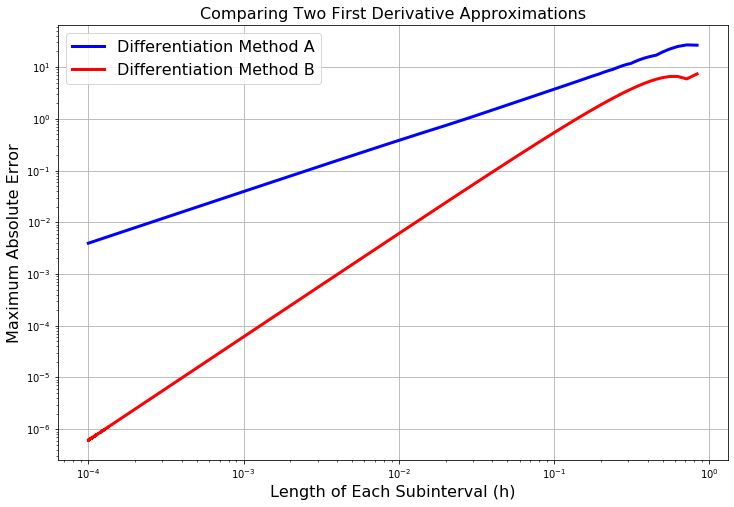
\includegraphics[width=0.75\linewidth]{images/Ch03_FirstDerivCompare} 

}

\caption{Maximum absolute error between the first derivative and two different approximations of the first derivative.}\label{fig:first-deriv-comparison}
\end{figure}

\begin{center}\rule{0.5\linewidth}{0.5pt}\end{center}

\hypertarget{the-second-derivative}{%
\subsection{The Second Derivative}\label{the-second-derivative}}

Now we'll search for an approximation of the second derivative. Again,
the game will be the same: experiment with the Taylor series and some algebra
with an eye toward getting the second derivative to pop out cleanly. This time we'll do the
algebra in such a way that the first derivative cancels.

From the previous problems you already have Taylor expansions of the
form \(f(x+h)\) and \(f(x-h)\). Let's summarize them here since you're going
to need them for future computations.
\[ \begin{aligned}
    f(x+h) &= f(x) + \frac{f'(x)}{1!} h + \frac{f''(x)}{2!} h^2 + \frac{f^{(3)}(x)}{3!}
    h^3 + \cdots \\
    f(x-h) &= f(x) - \frac{f'(x)}{1!} h + \frac{f''(x)}{2!} h^2 - \frac{f^{(3)}(x)}{3!}
    h^3 + \cdots \end{aligned} \]

\begin{center}\rule{0.5\linewidth}{0.5pt}\end{center}

\begin{exercise}
\protect\hypertarget{exr:unnamed-chunk-166}{}{\label{exr:unnamed-chunk-166} }The goal of
this problem is to use the Taylor series for \(f(x+h)\) and \(f(x-h)\) to
arrive at an approximation of the .

\begin{enumerate}
\def\labelenumi{\alph{enumi}.}
\item
  Add the Taylor series for \(f(x+h)\) and \(f(x-h)\) and combine all like
  terms. You should notice that several terms cancel.
  \[f(x+h) + f(x-h) = \underline{\hspace{3in}}.\]
\item
  Solve your answer in part (a) for \(f''(x)\).
  \[f''(x) = \frac{?? - 2 \cdot ?? + ??}{h^2} + \underline{\hspace{1in}}.\]
\item
  If we were to drop all of the terms after the fraction on the right-hand
  side of the previous result we would be introducing some error into the
  derivative computation. What does this tell us about the order of the error for the second derivative approximation scheme we just built?
\end{enumerate}
\end{exercise}

\begin{center}\rule{0.5\linewidth}{0.5pt}\end{center}

\begin{exercise}
\protect\hypertarget{exr:unnamed-chunk-167}{}{\label{exr:unnamed-chunk-167} }Again consider the function \(f(x) = \sin(x)(1 - x)\).

\begin{enumerate}
\def\labelenumi{\alph{enumi}.}
\item
  Calculate the derivative of this function and calculate the exact
  value of \(f''(1)\).
\item
  If we calcuate the second derivative with the central difference scheme that you built in the previous exericse using \(h = 0.5\) then we get a 4.115\% error. Stop now and verify this percent error calculation.
\item
  Based on our previous work with the order of the error in a numerical differentiation scheme, what do you predict the error will be if we calculate \(f''(1)\) with \(h = 0.25\)? With \(h = 0.05\)? With \(h = 0.005\)? Defend your answers.
\end{enumerate}
\end{exercise}

\begin{center}\rule{0.5\linewidth}{0.5pt}\end{center}

\begin{exercise}
\protect\hypertarget{exr:unnamed-chunk-168}{}{\label{exr:unnamed-chunk-168} }Write a Python function that takes a mathematical function and a domain and returns a second
order numerical approximation to the second derivative on the interval.
You should ALWAYS start by writing pseudo-code as comments in your function. As before, you should write your code without using any loops.
\end{exercise}

\begin{center}\rule{0.5\linewidth}{0.5pt}\end{center}

\begin{exercise}
\protect\hypertarget{exr:unnamed-chunk-169}{}{\label{exr:unnamed-chunk-169} }Test your second derivative code on the function
\(f(x) = \sin(x) - x\sin(x)\) by doing the following.

\begin{enumerate}
\def\labelenumi{\alph{enumi}.}
\item
  Find the analytic second derivative by hand.
\item
  Find the numerical second derivative with the code that you just
  wrote.
\item
  Find the absolute difference between your numerical second
  derivative and the actual second derivative. This is point-by-point
  subtraction so you should end up with a vector of errors.
\item
  Find the maximum of your errors.
\item
  Now we want to see how the code works if you change the number of
  points used. Build a plot showing the value of \(h\) on the horizontal
  axis and the maximum error on the vertical axis. You will need to
  write a loop that gets the error for many different values of \(h\).
  Finally, it is probably best to build this plot on a log-log scale.
\item
  Discuss what you see? How do you see the fact that the numerical
  second derivative is second order accurate?
\end{enumerate}
\end{exercise}

\begin{center}\rule{0.5\linewidth}{0.5pt}\end{center}

The table below summarizes the formulas that we have for derivatives thus far. The exercises at the end of this chapter contain several more derivative approximations. We will return to this idea when we study numerical differential equations in Chapter \ref{ch:odes}.

\begin{longtable}[]{@{}llll@{}}
\toprule
\begin{minipage}[b]{0.34\columnwidth}\raggedright
Derivative\strut
\end{minipage} & \begin{minipage}[b]{0.24\columnwidth}\raggedright
Formula\strut
\end{minipage} & \begin{minipage}[b]{0.17\columnwidth}\raggedright
Error\strut
\end{minipage} & \begin{minipage}[b]{0.14\columnwidth}\raggedright
Name\strut
\end{minipage}\tabularnewline
\midrule
\endhead
\begin{minipage}[t]{0.34\columnwidth}\raggedright
\(1^{st}\)\strut
\end{minipage} & \begin{minipage}[t]{0.24\columnwidth}\raggedright
\(f'(x) \approx \frac{f(x+h) - f(x)}{h}\)\strut
\end{minipage} & \begin{minipage}[t]{0.17\columnwidth}\raggedright
\(\mathcal{O}(h)\)\strut
\end{minipage} & \begin{minipage}[t]{0.14\columnwidth}\raggedright
Forward Difference\strut
\end{minipage}\tabularnewline
\begin{minipage}[t]{0.34\columnwidth}\raggedright
\(1^{st}\)\strut
\end{minipage} & \begin{minipage}[t]{0.24\columnwidth}\raggedright
\(f'(x) \approx \frac{f(x) - f(x-h)}{h}\)\strut
\end{minipage} & \begin{minipage}[t]{0.17\columnwidth}\raggedright
\(\mathcal{O}(h)\)\strut
\end{minipage} & \begin{minipage}[t]{0.14\columnwidth}\raggedright
Backward Difference\strut
\end{minipage}\tabularnewline
\begin{minipage}[t]{0.34\columnwidth}\raggedright
\(1^{st}\)\strut
\end{minipage} & \begin{minipage}[t]{0.24\columnwidth}\raggedright
\(f'(x) \approx \frac{f(x+h) - f(x-h)}{2h}\)\strut
\end{minipage} & \begin{minipage}[t]{0.17\columnwidth}\raggedright
\(\mathcal{O}(h^2)\)\strut
\end{minipage} & \begin{minipage}[t]{0.14\columnwidth}\raggedright
Centered Difference\strut
\end{minipage}\tabularnewline
\begin{minipage}[t]{0.34\columnwidth}\raggedright
\(2^{nd}\)\strut
\end{minipage} & \begin{minipage}[t]{0.24\columnwidth}\raggedright
\(f''(x) \approx \frac{f(x+h) - 2f(x) + f(x-h)}{h^2}\)\strut
\end{minipage} & \begin{minipage}[t]{0.17\columnwidth}\raggedright
\(\mathcal{O}(h^2)\)\strut
\end{minipage} & \begin{minipage}[t]{0.14\columnwidth}\raggedright
Centered Difference\strut
\end{minipage}\tabularnewline
\bottomrule
\end{longtable}

\begin{center}\rule{0.5\linewidth}{0.5pt}\end{center}

\begin{exercise}
\protect\hypertarget{exr:unnamed-chunk-170}{}{\label{exr:unnamed-chunk-170} }Let \(f(x)\) be a twice differentiable function. We are interested in the
first and second derivative of the function \(f\) at the point \(x = 1.74\).
Use what you have learned in this section to answer the following
questions. (For clarity, you can think of ``\(f\)'' as a different function
in each of the following questions \ldots it doesn't really matter exactly
what function \(f\) is.)

\begin{enumerate}
\def\labelenumi{\alph{enumi}.}
\item
  Johnny used a numerical first derivative scheme with \(h = 0.1\) to
  approximate \(f'(1.74)\) and found an abolute percent error of 3.28\%.
  He then used \(h=0.01\) and found an absolute percent error of 0.328\%.
  What was the order of the error in his first derivative scheme? How
  can you tell?
\item
  Betty used a numerical first derivative scheme with \(h = 0.2\) to
  approximate \(f'(1.74)\) and found an absolute percent error of 4.32\%.
  She then used \(h=0.1\) and found an absolute percent error of 1.08\%.
  What numerical first derivative scheme did she likely use?
\item
  Shelby did the computation
  \[f'(1.74) \approx \frac{f(1.78) - f(1.74)}{0.04}\] and found an
  absolute percent error of 2.93\%. If she now computes
  \[f'(1.74) \approx \frac{f(1.75) - f(1.74)}{0.01}\] what will the
  new absolute percent error be?
\item
  Harry wants to compute \(f''(1.74)\) to within 1\% using a central
  difference scheme. He tries \(h=0.25\) and gets an absolute percent
  error of 3.71\%. What \(h\) should he try next so that his absolute
  percent error is less than (but close to) 1\%?
\end{enumerate}
\end{exercise}

\begin{center}\rule{0.5\linewidth}{0.5pt}\end{center}

\hypertarget{integration}{%
\section{Integration}\label{integration}}

Now we begin our work on the second principle computation of Calculus: evaluating a definite integral. Remember that a single-variable definite integral can be interpreted as the signed area between the curve and the \(x\) axis. In this section we will study three different techniques for approximating the value of a definite integral.

\begin{center}\rule{0.5\linewidth}{0.5pt}\end{center}

\begin{exercise}
\protect\hypertarget{exr:unnamed-chunk-171}{}{\label{exr:unnamed-chunk-171} }Consider the shaded area of the region under the function plotted in
Figure \ref{fig:integration-ex1} between \(x=0\) and \(x=2\).

\begin{enumerate}
\def\labelenumi{\arabic{enumi}.}
\item
  What rectangle with area 6 gives an upper bound for the area under
  the curve? Can you give a better upper bound?
\item
  Why must the area under the curve be greater than 3?
\item
  Is the area greater than 4? Why/Why not?
\item
  Work with your partner to give an estimate of the area and provide
  an estimate for the amount of error that you're making.
\end{enumerate}
\end{exercise}

\begin{figure}

{\centering 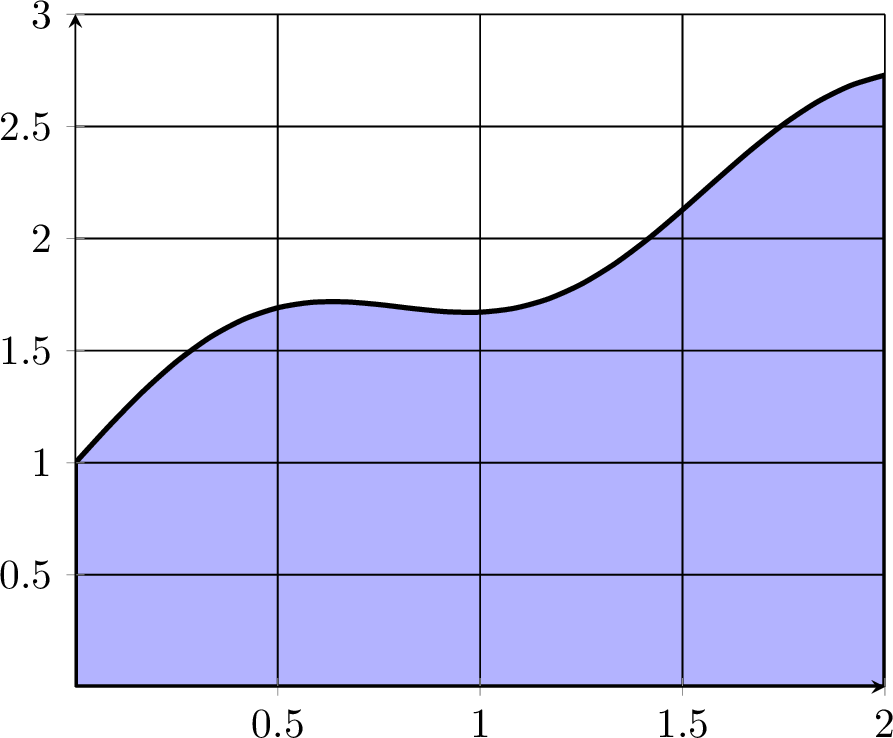
\includegraphics[width=0.45\linewidth]{images/Ch03_InitialIntegral} 

}

\caption{A sample integration}\label{fig:integration-ex1}
\end{figure}

\begin{center}\rule{0.5\linewidth}{0.5pt}\end{center}

\hypertarget{riemann-sums}{%
\subsection{Riemann Sums}\label{riemann-sums}}

In this subsection we will build our first method for approximating definite integrals.
Recall from Calculus that the definition of the Riemann integral is
\[\begin{aligned}
    \int_a^b f(x) dx = \lim_{\Delta x \to 0} \sum_{j=1}^N f(x_j) \Delta x
    \label{eqn:Riemann_integral}\end{aligned}\]
where \(N\) is the number
of sub intervals on the interval \([a,b]\) and \(\Delta x\) is the width of
the interval. As with differentiation, we can remove the limit and have
a decent approximation of the integral so long as \(N\) is large (or equivalently, if \(\Delta x\) is small).
\[\int_a^b f(x) dx \approx \sum_{j=1}^N f(x_j) \Delta x.\] You are
likely familiar with this approximation of the integral from Calculus.
The value of \(x_j\) can be chosen anywhere within the sub interval and
three common choices are to use the left endpoint, the midpoint, and the
right endpoint.

We see a depiction of this in Figure \ref{fig:integral-with-rectangles}.

\begin{figure}

{\centering 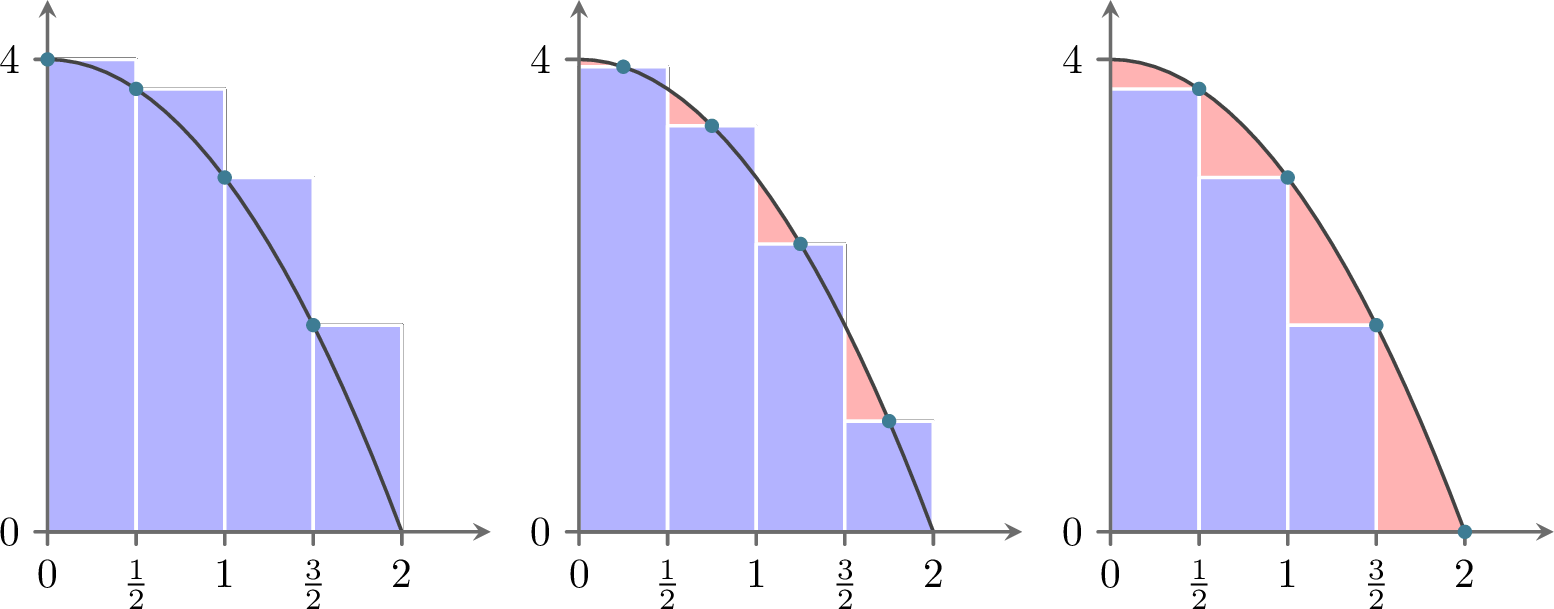
\includegraphics[width=0.8\linewidth]{images/Ch03_ThreeRiemannSums} 

}

\caption{Right-aligned Riemann sums, midpoint-aligned Riemann sums, and left-aligned Riemann sums}\label{fig:integral-with-rectangles}
\end{figure}

Clearly, the more rectangles we choose the closer the sum of the areas
of the rectangles will get to the integral.

\begin{center}\rule{0.5\linewidth}{0.5pt}\end{center}

\begin{exercise}
\protect\hypertarget{exr:unnamed-chunk-172}{}{\label{exr:unnamed-chunk-172} }Write code to approximate an integral with Riemann sums. You should ALWAYS
start by writing pseudo-code as comments in your function. Your Python function
should accept a Python Function, a lower
bound, an upper bound, the number of subintervals, and an optional input
that allows the user to designate whether they want left, right, or
midpoint rectangles. Test your code on several functions for which you know the integral. You
should write your code without any loops.
\end{exercise}

\begin{center}\rule{0.5\linewidth}{0.5pt}\end{center}

\begin{exercise}
\protect\hypertarget{exr:unnamed-chunk-173}{}{\label{exr:unnamed-chunk-173} }Consider the function \(f(x) = \sin(x)\). We know the antiderivative for this function, \(F(x) = -\cos(x) + C\), but in this question we are going to get a sense of the order of the error when doing Riemann Sum integration.

\begin{enumerate}
\def\labelenumi{\alph{enumi}.}
\item
  Find the exact value of \[\int_0^{1} f(x) dx.\]
\item
  Now build a Riemann Sum approximation (using your code) with various
  values of \(\Delta x\). For all of your approximation use
  left-justified rectangles. Fill in the table with your results.
\end{enumerate}

\begin{longtable}[]{@{}llll@{}}
\toprule
\(\Delta x\) & Approx. Integral & Exact Integral & Abs. Percent Error\tabularnewline
\midrule
\endhead
\(2^{-2} = 0.25\) & & &\tabularnewline
\(2^{-3} = 0.125\) & & &\tabularnewline
\(2^{-4}\) & & &\tabularnewline
\(2^{-5}\) & & &\tabularnewline
\(2^{-6}\) & & &\tabularnewline
\(2^{-7}\) & & &\tabularnewline
\(2^{-8}\) & & &\tabularnewline
\(2^{-9}\) & & &\tabularnewline
\bottomrule
\end{longtable}

\begin{enumerate}
\def\labelenumi{\alph{enumi}.}
\setcounter{enumi}{2}
\item
  There was nothing really special about powers of 2 in part (b) of
  this problem. Examine other sequences of \(\Delta x\) with a goal
  toward answering the question:\\
  \emph{If we find an approximation of the integral with a fixed \(\Delta x\) and find an absolute percent error, then what would happen to the absolute percent error if we divide \(\Delta x\) by some positive constant \(M\)?}
\item
  What is the apparent approximation error of the Riemann Sum method
  using left-justified rectangles.
\end{enumerate}
\end{exercise}

\begin{center}\rule{0.5\linewidth}{0.5pt}\end{center}

\begin{exercise}
\protect\hypertarget{exr:unnamed-chunk-174}{}{\label{exr:unnamed-chunk-174} }Repeat the previous problem using right-justified rectangles.
\end{exercise}

\begin{center}\rule{0.5\linewidth}{0.5pt}\end{center}

\begin{theorem}
\protect\hypertarget{thm:unnamed-chunk-175}{}{\label{thm:unnamed-chunk-175} }In approximating the integral \(\int_a^b f(x) dx\) with a fixed interval
width \(\Delta  x\) we find an absolute percent error \(P\).

\begin{itemize}
\item
  If we use left rectangles and an interval width of
  \(\frac{\Delta x}{M}\) then the absolute percent error will be
  approximately \(\underline{\hspace{1in}}\).
\item
  If we use right rectangles and an interval width of
  \(\frac{\Delta x}{M}\) then the absolute percent error will be
  approximately \(\underline{\hspace{1in}}\).
\end{itemize}
\end{theorem}

\begin{center}\rule{0.5\linewidth}{0.5pt}\end{center}

\begin{exercise}
\protect\hypertarget{exr:unnamed-chunk-176}{}{\label{exr:unnamed-chunk-176} }The previous theorem could be stated in an equivalent way.

In approximating the integral \(\int_a^b f(x) dx\) with a fixed interval
number of subintervals we find an absolute percent error \(P\).

\begin{itemize}
\item
  If we use left rectangles and \(M\) times as many subintervals then
  the absolute percent error will be approximately \(\underline{\hspace{1in}}\).
\item
  If we use right rectangles and \(M\) times as many subintervals then
  the absolute percent error will be approximately \(\underline{\hspace{1in}}\).
\end{itemize}
\end{exercise}

\begin{center}\rule{0.5\linewidth}{0.5pt}\end{center}

\begin{exercise}
\protect\hypertarget{exr:unnamed-chunk-177}{}{\label{exr:unnamed-chunk-177} }Create a plot with the width of the subintervals on the horizontal axis
and the absolute error between your (left) Riemann sum calculation and
the exact integral for a known definite integral. Your plot should be on
a log-log scale. Based on your plot, what is the approximate order of
the error in the Riemann sum approximation?
\end{exercise}

\begin{center}\rule{0.5\linewidth}{0.5pt}\end{center}

\hypertarget{trapezoidal-rule}{%
\subsection{Trapezoidal Rule}\label{trapezoidal-rule}}

Now let's turn our attention to some slightly better algorithms for
calculating the value of a definite integral: The Trapezoidal Rule and
Simpson's Rule. There are many others, but in practice these two are
relatively easy to implement and have reasonably good error
approximations. To motivate the idea of the Trapezoid rule consider
Figure \ref{fig:trap-motivation}. It is plain to see that trapezoids
will make better approximations than rectangles at least in this
particular case. Another way to think about using trapezoids, however,
is to see the top side of the trapezoid as a secant line connecting two
points on the curve. As \(\Delta x\) gets arbitrarily small, the secant
lines become better and better approximations for tangent lines and are
hence arbitrarily good approximations for the curve. For these reasons
it seems like we should investigate how to systematically approximate
definite integrals via trapezoids.

\begin{figure}

{\centering 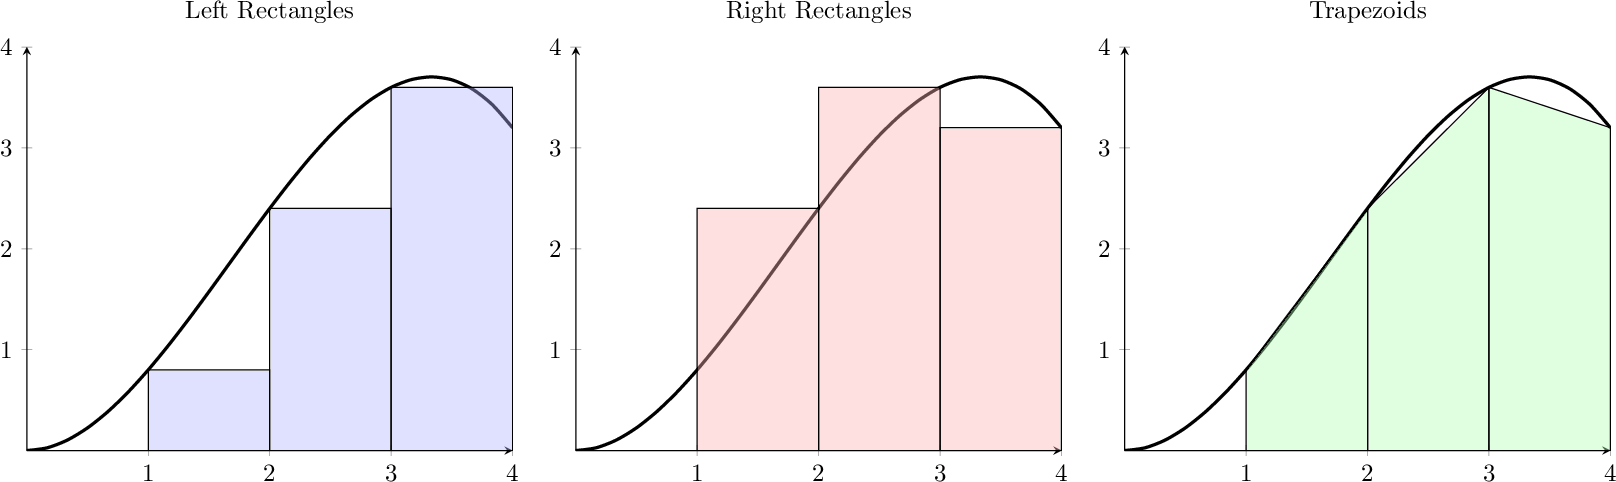
\includegraphics[width=0.9\linewidth]{images/Ch03_Trapezoidal1} 

}

\caption{Motivation for using trapezoids to approximate a definite integral.}\label{fig:trap-motivation}
\end{figure}

\begin{center}\rule{0.5\linewidth}{0.5pt}\end{center}

\begin{exercise}
\protect\hypertarget{exr:unnamed-chunk-178}{}{\label{exr:unnamed-chunk-178} }Consider a single trapezoid approximating the area under a curve. From
geometry we recall that the area of a trapezoid is
\[A = \frac{1}{2}\left( b_1 + b_2 \right) h\] where \(b_1, b_2\) and \(h\)
are marked in Figure \ref{fig:trapezoidal-2}. The function shown in the picture is
\(f(x) = \frac{1}{5} x^2 (5-x)\). Find the area of the shaded region as an
approximation to \[\int_1^4 \left( \frac{1}{5} x^2 (5-x) \right) dx.\]

Now use the same idea with \(h = \Delta x = 1\) from Figure \ref{fig:trap-motivation} to approximate the area under the function \(f(x) = \frac{1}{5}x^2(5-x)\) between \(x=1\) and \(x=4\) using three trapezoids.
\end{exercise}

\begin{figure}

{\centering 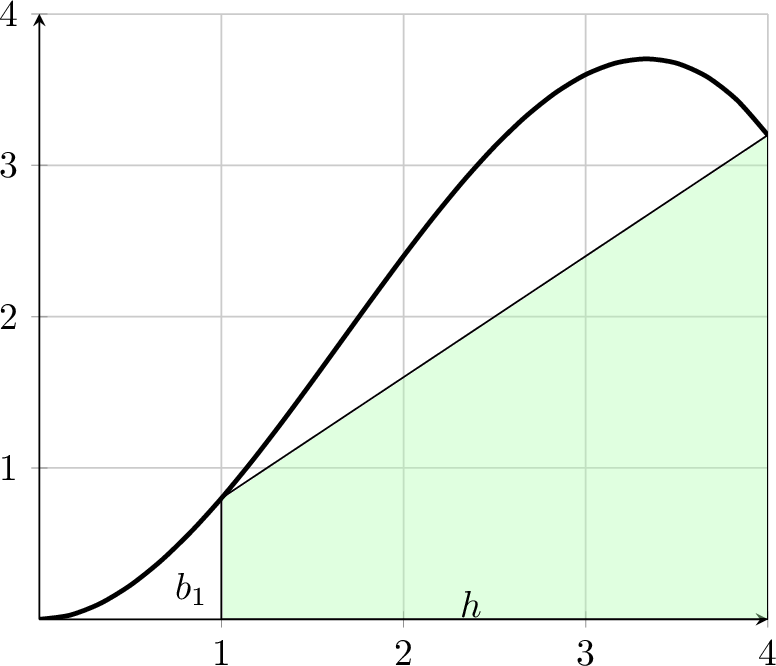
\includegraphics[width=0.4\linewidth]{images/Ch03_Trapezoidal2} 

}

\caption{A single trapezoid to approximate area under a curve.}\label{fig:trapezoidal-2}
\end{figure}

\begin{center}\rule{0.5\linewidth}{0.5pt}\end{center}

\begin{exercise}
\protect\hypertarget{exr:unnamed-chunk-179}{}{\label{exr:unnamed-chunk-179} }Consider the function \(f(x) = \frac{1}{5}x^2(5-x)\) again.

\begin{enumerate}
\def\labelenumi{\alph{enumi}.}
\item
  Work out the exact value of the definite integral by hand.
\item
  Summarize your answers to the previous problems in the following
  table then extend the data that you have for smaller and smaller
  values of \(\Delta x\).
\end{enumerate}

\begin{longtable}[]{@{}llll@{}}
\toprule
\(\Delta x\) & Approx. Integral & Exact Integral & Abs. \% Error\tabularnewline
\midrule
\endhead
\(3\) & & &\tabularnewline
\(1\) & & &\tabularnewline
\(1/3\) & & &\tabularnewline
\(1/9\) & & &\tabularnewline
\(\vdots\) & \(\vdots\) & \(\vdots\) & \(\vdots\)\tabularnewline
\bottomrule
\end{longtable}

\begin{enumerate}
\def\labelenumi{\alph{enumi}.}
\setcounter{enumi}{2}
\tightlist
\item
  From the table that you built in part (b), what do you conjecture is
  the order of the approximation error for the trapezoid method?
\end{enumerate}
\end{exercise}

\begin{center}\rule{0.5\linewidth}{0.5pt}\end{center}

\begin{definition}[The Trapezoidal Rule]
\protect\hypertarget{def:trapezoidal}{}{\label{def:trapezoidal} \iffalse (The Trapezoidal Rule) \fi{} }We want to approximate \(\displaystyle \int_a^b f(x) dx\). One of the
simplest ways is to approximate the area under the function with a
trapezoid. Recall from basic geometry that area of a trapezoid is
\(A = \frac{1}{2} (b_1 + b_2) h\). In terms of the integration problem we
can do the following:

\begin{enumerate}
\def\labelenumi{\alph{enumi}.}
\item
  First partition \([a,b]\) into the set
  \(\{x_0=a, x_1, x_2, \ldots, x_{n-1},  x_n=b\}\).
\item
  On each part of the partition approximate the area with a trapezoid:
  \[A_j = \frac{1}{2} \left[ f(x_j) + f(x_{j-1}) \right]\left(
              x_j - x_{j-1} \right)\]
\item
  Approximate the integral as \[\int_a^b f(x) dx = \sum_{j=1}^n A_j\]
\end{enumerate}
\end{definition}

\begin{center}\rule{0.5\linewidth}{0.5pt}\end{center}

\begin{exercise}
\protect\hypertarget{exr:unnamed-chunk-180}{}{\label{exr:unnamed-chunk-180} }Write code to give the trapezoidal rule approximation for the definite
integral \(\int_a^b f(x) dx\). Test your code on functions where you know
the definite area. Then test your code on functions where you have
approximated the area by examining a plot (i.e.~you have a visual
estimate of the area).
\end{exercise}

\begin{center}\rule{0.5\linewidth}{0.5pt}\end{center}

\begin{exercise}
\protect\hypertarget{exr:unnamed-chunk-181}{}{\label{exr:unnamed-chunk-181} }Use the code that you wrote in the previous problem to test your
conjecture about the order of the approximation error for the trapezoid
rule. Integrate the function \(f(x) = \sin(x)\) from \(x=0\) to \(x=1\) with more and more trapezoids. In
each case compare to the exact answer and find the absolute percent
error. The goal is to answer the question:\\
\emph{If we calculate the definite integral with a fixed \(\Delta x\) and get an
absolute percent error, \(P\), then what absolute percent error will we get
if we use a width of \(\Delta x / M\) for some positive number \(M\)?}
\end{exercise}

\begin{center}\rule{0.5\linewidth}{0.5pt}\end{center}

\hypertarget{simpsons-rule}{%
\subsection{Simpsons Rule}\label{simpsons-rule}}

The trapezoidal rule does a decent job approximating integrals, but
ultimately you are using linear functions to approximate \(f(x)\) and the
accuracy may suffer if the step size is too large or the function too
non-linear. You likely notice that the trapezoidal rule will give an
exact answer if you were to integrate a linear or constant function. A
potentially better approach would be to get an integral that evaluates
quadratic functions exactly. In order to do this we need to evaluate the
function at three points (not two like the trapezoidal rule). Let's
integrate a function \(f(x)\) on the interval \([a,b]\) by using the three
points \((a,f(a))\), \((m,f(m))\), and \((b,f(b))\) where \(m=\frac{a+b}{2}\) is
the midpoint of the two boundary points.

We want to find constants \(A_1\), \(A_2\), and \(A_3\) such that the integral
\(\int_a^b f(x) dx\) can be written as a linear combination of \(f(a)\),
\(f(m)\), and \(f(b)\). Specifically, we want constants \(A_1\), \(A_2\), and
\(A_3\) such that
\[\int_a^b f(x) dx = A_1 f(a) + A_2 f(m) + A_3 f(b)\]
is for all constant, linear, and quadratic functions. This would
guarantee that we have an exact integration method for all polynomials
of order 2 or less but should serve as a decent approximation if the
function is not quadratic.

\begin{center}\rule{0.5\linewidth}{0.5pt}\end{center}

\begin{exercise}
\protect\hypertarget{exr:unnamed-chunk-182}{}{\label{exr:unnamed-chunk-182} }Draw a picture showing what the previous two paragraphs discussed.
\end{exercise}

\begin{center}\rule{0.5\linewidth}{0.5pt}\end{center}

\begin{exercise}
\protect\hypertarget{exr:unnamed-chunk-183}{}{\label{exr:unnamed-chunk-183} }Follow these steps to find \(A_1\), \(A_2\), and \(A_3\).

\begin{enumerate}
\def\labelenumi{\alph{enumi}.}
\item
  Prove that \[\int_a^b 1 dx = b-a = A_1 + A_2 + A_3.\]
\item
  Prove that
  \[\int_a^b x dx = \frac{b^2 - a^2}{2} = A_1 a + A_2 \left( \frac{a+b}{2} \right) + A_3
          b.\]
\item
  Prove that
  \[\int_a^b x^2 dx = \frac{b^3 - a^3}{3} = A_1 a^2 + A_2 \left( \frac{a+b}{2} \right)^2
          + A_3 b^2.\]
\item
  Now solve the linear system of equations to prove that
  \[A_1 = \frac{b-a}{6}, \quad A_2 = \frac{4(b-a)}{6}, \quad \text{and} \quad
          A_3 = \frac{b-a}{6}.\]
\end{enumerate}
\end{exercise}

\begin{center}\rule{0.5\linewidth}{0.5pt}\end{center}

\begin{exercise}
\protect\hypertarget{exr:unnamed-chunk-184}{}{\label{exr:unnamed-chunk-184} }At this point we can see that an integral can be approximated as
\[\int_a^b f(x) dx \approx \left( \frac{b-a}{6} \right) \left( f(a) + 4f\left(
\frac{a+b}{2} \right) + f(b) \right)\] and the technique will give an
exact answer for any polynomial of order 2 or below.

Verify the previous sentence by integrating \(f(x) = 1\), \(f(x) = x\) and
\(f(x) = x^2\) by hand on the interval \([0,1]\) and using the approximation
formula
\[\int_a^b f(x) dx \approx \left( \frac{b-a}{6} \right) \left( f(a) + 4f\left(
\frac{a+b}{2} \right) + f(b) \right).\]

\begin{enumerate}
\def\labelenumi{\alph{enumi}.}
\item
  Use the method described above to approximate the area under the
  curve \(f(x) = (1/5) x^2 (5-x)\) on the interval \([1,4]\). To be clear,
  you will be using the points \(a=1, m=2.5\), and \(b=4\) in the above
  derivation.
\item
  Next find the exact area under the curve \(g(x) = (-1/2)x^2 +3.3x -2\)
  on the interval \([1,4]\).
\item
  What do you notice about the two areas? What does this sample
  problem tell you about the formula that we derived above?
\end{enumerate}
\end{exercise}

\begin{center}\rule{0.5\linewidth}{0.5pt}\end{center}

To make the punchline of the previous exercises a bit more clear, using the formula
\[\int_a^b f(x) dx \approx \left( \frac{a-b}{6} \right) \left( f(a) + 4 f(m) + f(b)
\right)\] is the same as fitting a parabola to the three points
\((a,f(a))\), \((m,f(m))\), and \((b,f(b))\) and finding the area under the
parabola exactly. That is exactly the step up from the trapezoid rule
and Riemann sums that we were after:

\begin{itemize}
\tightlist
\item
  Riemann sums approximate the function with constant functions,
\item
  the trapezoid rule uses linear functions, and
\item
  now we have a method for approximating with parabolas.
\end{itemize}

To improve upon this idea we now examine the problem of partitioning the
interval \([a,b]\) into small pieces and running this process on each
piece. This is called Simpson's Rule for integration.

\begin{center}\rule{0.5\linewidth}{0.5pt}\end{center}

\begin{definition}[Simpson's Rule]
\protect\hypertarget{def:simpsons-rule}{}{\label{def:simpsons-rule} \iffalse (Simpson's Rule) \fi{} }Now we put the process explained above into a form that can be coded to
approximate integrals. We call this method Simpson's Rule after \href{https://en.wikipedia.org/wiki/Thomas_Simpson}{Thomas Simpson (1710-1761)} who, by the way, was a basket weaver in his day job so he could pay the bills and keep doing math.

\begin{enumerate}
\def\labelenumi{\alph{enumi}.}
\item
  First partition \([a,b]\) into the set
  \(\{x_0=a, x_1, x_2, \ldots, x_{n-1},  x_n=b\}\).
\item
  On each part of the partition approximate the area with a parabola:
  \[A_j = \frac{1}{6} \left[ f(x_j) + 4 f\left( \frac{x_j+x_{j-1}}{2} \right) +
                  f(x_{j-1}) \right]\left( x_j - x_{j-1} \right)\]
\item
  Approximate the integral as \[\int_a^b f(x) dx = \sum_{j=1}^n A_j\]
\end{enumerate}
\end{definition}

\begin{center}\rule{0.5\linewidth}{0.5pt}\end{center}

\begin{exercise}
\protect\hypertarget{exr:unnamed-chunk-185}{}{\label{exr:unnamed-chunk-185} }We have spent a lot of time over the past many pages building
approximations of the order of the error for numerical integration and
differentiation schemes. It is now up to you.\\
Build a numerical experiment that allows you to conjecture the order of
the approximation error for Simpson's rule. Remember that the goal is to
answer the question:\\
\emph{If I approximate the integral with a fixed \(\Delta x\) and find an absolute percent error of \(P\), then what will the absolute percent error be using a width of \(\Delta x / M\)?}
\end{exercise}

\begin{center}\rule{0.5\linewidth}{0.5pt}\end{center}

\begin{exercise}
\protect\hypertarget{exr:unnamed-chunk-186}{}{\label{exr:unnamed-chunk-186} }Write a Python function that implements Simpson's Rule. You should ALWAYS start by writing pseudo-code as comments in your file. You shouldn't need a loop in your function.
\end{exercise}

\begin{center}\rule{0.5\linewidth}{0.5pt}\end{center}

\begin{exercise}
\protect\hypertarget{exr:unnamed-chunk-187}{}{\label{exr:unnamed-chunk-187} }Test your function on known integrals and approximate the order of the error based on the mesh size.
\end{exercise}

\begin{center}\rule{0.5\linewidth}{0.5pt}\end{center}

Thus far we have three numerical approximations for definite integrals:
Riemann sums (with rectangles), the trapezoidal rule, and Simpsons's
rule. There are MANY other approximations for integrals and we leave the
further research to the curious reader.

\begin{center}\rule{0.5\linewidth}{0.5pt}\end{center}

\begin{theorem}[Numerical Integration Schemes]
\protect\hypertarget{thm:num-int}{}{\label{thm:num-int} \iffalse (Numerical Integration Schemes) \fi{} }Let \(f(x)\) be a continuous function on the interval \([a,b]\). The integral \(\int_a^b f(x) dx\) can be approximated with any of the following.
\[\begin{aligned}
       &\text{Riemann Sum: }  \int_a^b f(x) dx \approx \sum_{j=1}^N f(x_j) \Delta x \\
       & \qquad \text{Error for Riemann Sums: } \mathcal{O}(\Delta x) \\
       &\text{Trapezoidal Rule: }  \int_a^b f(x) dx \approx \frac{1}{2} \sum_{j=1}^N
       \left( f(x_j) + f(x_{j-1}) \right) \Delta x \\
       & \qquad \text{Error for Trapezoidal Rule: } \mathcal{O}(\Delta x^2) \\
       &\text{Simpson's Rule: }  \int_a^b f(x) dx \approx \frac{1}{6} \sum_{j=1}^N \left(
       f(x_j) + 4 f\left( \frac{x_j + x_{j-1}}{2} \right) + f(x_{j-1}) \right) \Delta x \\
       & \qquad \text{Error for Simpson's Rule: } \mathcal{O}(\Delta x^4) \\
    \end{aligned}\] where \(\Delta x = x_j - x_{j-1}\) and \(N\) is the
number of subintervals.
\end{theorem}

\begin{center}\rule{0.5\linewidth}{0.5pt}\end{center}

\begin{exercise}
\protect\hypertarget{exr:unnamed-chunk-188}{}{\label{exr:unnamed-chunk-188} }Theorem \ref{thm:num-int} simply states the error rates for our three
primary integration schemes. For this problem you need to empirically
verify these error rates. Use the integration problem and exact answer
\[\int_0^{\pi/4} e^{3x} \sin(2x) dx = \frac{3}{13} e^{3\pi/4} + \frac{2}{13}\]
and write code that produces a log-log error plot with \(\Delta x\) on the
horizontal axis and the absolute error on the vertical axis. Fully
explain how the error rates show themselves in your plot.
\end{exercise}

\begin{center}\rule{0.5\linewidth}{0.5pt}\end{center}

\hypertarget{optimization}{%
\section{Optimization}\label{optimization}}

\hypertarget{single-variable-optimization}{%
\subsection{Single Variable Optimization}\label{single-variable-optimization}}

You likely recall that one of the major applications of Calculus was to
solve optimization problems -- find the value of \(x\) which makes some
function as big or as small as possible. The process itself can
sometimes be rather challenging due to either the modeling aspect of the
problems and/or the fact that the differentiation might be quite
cumbersome. In this section we will revisit those problems from
Calculus, but our goal will be to build a numerical method for the
Calculus step in hopes to avoid the messy algebra and differentiation.

\begin{center}\rule{0.5\linewidth}{0.5pt}\end{center}

\begin{exercise}
\protect\hypertarget{exr:cardboard-problem}{}{\label{exr:cardboard-problem} }A piece of cardboard measuring 20cm by 20cm is to be cut so that it can be folded into a box without a lid (see Figure \ref{fig:cardboard}). We want to find the size of the cut, \(x\), that maximizes the volume of the box.

\begin{enumerate}
\def\labelenumi{\alph{enumi}.}
\item
  Write a function for the volume of the box resulting from a cut of
  size \(x\). What is the domain of your function?
\item
  We know that we want to maximize this function so go through the
  full Calculus exercise to find the maximum:

  \begin{itemize}
  \item
    take the derivative
  \item
    set it to zero
  \item
    find the critical points
  \item
    test the critical points and the boundaries of the domain using
    the extreme value theorem to determine the \(x\) that gives the
    maximum.
  \end{itemize}
\end{enumerate}
\end{exercise}

\begin{figure}

{\centering 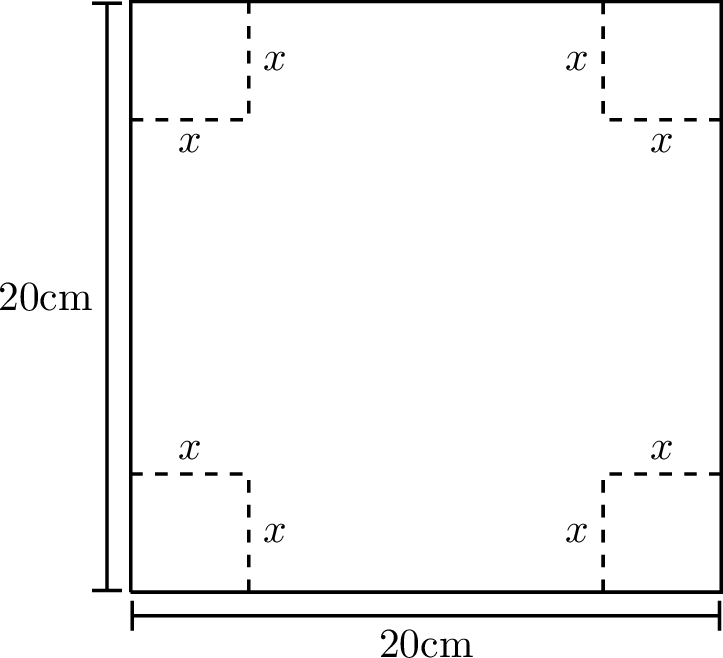
\includegraphics[width=0.4\linewidth]{images/Ch03_CardboardBox} 

}

\caption{Folds to make a cardboard box}\label{fig:cardboard}
\end{figure}

\begin{center}\rule{0.5\linewidth}{0.5pt}\end{center}

Now we'll propose a few numerical techniques that can approximate the
solution to these types of problems. The basic ideas are simple!

\begin{exercise}
\protect\hypertarget{exr:unnamed-chunk-189}{}{\label{exr:unnamed-chunk-189} }If you were blind folded and standing on a hill could you find the top of the hill? (assume no trees and no cliffs \ldots this isn't supposed to be dangerous) How would you do it? Explain your technique clearly.
\end{exercise}

\begin{center}\rule{0.5\linewidth}{0.5pt}\end{center}

\begin{exercise}
\protect\hypertarget{exr:unnamed-chunk-190}{}{\label{exr:unnamed-chunk-190} }If you were blind folded and standing on a crater on the moon could you find the lowest point? How would you do it? Remember that you can hop as far as you like \ldots because gravity \ldots but sometimes that's not a great thing because you could hop too far.
\end{exercise}

\begin{center}\rule{0.5\linewidth}{0.5pt}\end{center}

The intuition of numerical optimization schemes is typically to
visualize the function that you're trying to minimize or maximize and
think about either climbing the hill to the top (maximization) or
descending the hill to the bottom (minimization).

\begin{center}\rule{0.5\linewidth}{0.5pt}\end{center}

\begin{exercise}
\protect\hypertarget{exr:unnamed-chunk-191}{}{\label{exr:unnamed-chunk-191} }Let's turn your intuition into an algorithm. If \(f(x)\) is the function that you are trying to maximize then turn your algorithm from the previous problems into a step-by-step algorithm which could be coded. Then try out your code on the function
\[f(x) = e^{-x^2} + \sin(x^2)\] to see if your algorithm can find the
local maximum near \(x \approx 1.14\).
\end{exercise}

\begin{center}\rule{0.5\linewidth}{0.5pt}\end{center}

Some of the most common algorithms are listed below. Read through them and see which one(s) you ended up recreating? The intuition for these algorithms is pretty darn simple -- travel uphill if you want to maximize -- travel downhill if you want to minimize.

\begin{center}\rule{0.5\linewidth}{0.5pt}\end{center}

\begin{definition}[Derivative Free Optimization]
\protect\hypertarget{def:unnamed-chunk-192}{}{\label{def:unnamed-chunk-192} \iffalse (Derivative Free Optimization) \fi{} }Let \(f(x)\) be the objective function which you are seeking to maximize
(or minimize).

\begin{itemize}
\item
  Pick a starting point, \(x_0\), and find the value of your objective
  function at this point, \(f(x_0)\).
\item
  Pick a small step size (say, \(\Delta x \approx 0.01\)).
\item
  Calculate the objective function one step to the left and one step
  to the right from your starting point. Which ever point is larger
  (if you're seeking a maximum) is the point that you keep for your
  next step.
\item
  Iterate (decide on a good stopping rule)
\end{itemize}
\end{definition}

\begin{center}\rule{0.5\linewidth}{0.5pt}\end{center}

\begin{exercise}
\protect\hypertarget{exr:unnamed-chunk-193}{}{\label{exr:unnamed-chunk-193} }Write code to implement the 1D derivative free optimization algorithm and use it to solve Exercise \ref{exr:cardboard-problem}. Compare your answer to the analytic solution.
\end{exercise}

\begin{center}\rule{0.5\linewidth}{0.5pt}\end{center}

\begin{definition}[Gradient Descent/Ascent]
\protect\hypertarget{def:unnamed-chunk-194}{}{\label{def:unnamed-chunk-194} \iffalse (Gradient Descent/Ascent) \fi{} }Let \(f(x)\) be the objective function which you are seeking to maximize (or minimize).

\begin{itemize}
\item
  Find the derivative of your objective function, \(f'(x)\).
\item
  Pick a starting point, \(x_0\).
\item
  Pick a small control parameter, \(\alpha\) (in machine learning this
  parameter is called the ``learning rate'' for the gradient descent
  algorithm).
\item
  Use the iteration \(x_{n+1} = x_n + \alpha f'(x_n)\) if you're
  maximizing. Use the iteration \(x_{n+1} = x_n - \alpha f'(x_n)\) if
  you're minimizing.
\item
  Iterate (decide on a good stopping rule)
\end{itemize}
\end{definition}

\begin{center}\rule{0.5\linewidth}{0.5pt}\end{center}

\begin{exercise}
\protect\hypertarget{exr:unnamed-chunk-195}{}{\label{exr:unnamed-chunk-195} }Write code to implement the 1D gradient descent algorithm and use it to solve Exercise \ref{exr:cardboard-problem}. Compare your answer to the analytic solution.
\end{exercise}

\begin{center}\rule{0.5\linewidth}{0.5pt}\end{center}

\begin{definition}[Monte-Carlo Search]
\protect\hypertarget{def:unnamed-chunk-196}{}{\label{def:unnamed-chunk-196} \iffalse (Monte-Carlo Search) \fi{} }Let \(f(x)\) be the objective function which you are seeking to maximize
(or minimize).

\begin{itemize}
\item
  Pick many (perhaps several thousand!) different \(x\) values.
\item
  Find the value of the objective function at every one of these
  points (Hint: use lists, not loops)
\item
  Keep the \(x\) value that has the largest (or smallest if you're
  minimizing) value of the objective function.
\item
  Iterate many times and compare the function value in each iteration
  to the previous best function value
\end{itemize}
\end{definition}

\begin{center}\rule{0.5\linewidth}{0.5pt}\end{center}

\begin{exercise}
\protect\hypertarget{exr:unnamed-chunk-197}{}{\label{exr:unnamed-chunk-197} }Write code to implement the 1D monte carlo search algorithm and use it to solve Exercise \ref{exr:cardboard-problem}. Compare your answer to the analytic solution.
\end{exercise}

\begin{center}\rule{0.5\linewidth}{0.5pt}\end{center}

\begin{definition}[Optimization via Numerical Root Finding]
\protect\hypertarget{def:unnamed-chunk-198}{}{\label{def:unnamed-chunk-198} \iffalse (Optimization via Numerical Root Finding) \fi{} }Let \(f(x)\) be the objective function which you are seeking to maximize (or minimize).

\begin{itemize}
\item
  Find the derivative of your objective function.
\item
  Set the derivative to zero and use a numerical root finding method
  (such as bisection or Newton) to find the critical point.
\item
  Use the extreme value theorem to determine if the critical point or
  one of the endpoints is the maximum (or minimum).
\end{itemize}
\end{definition}

\begin{center}\rule{0.5\linewidth}{0.5pt}\end{center}

\begin{exercise}
\protect\hypertarget{exr:unnamed-chunk-199}{}{\label{exr:unnamed-chunk-199} }Write code to implement the 1D numerical root finding optimization algorithm and use it to solve Exercise \ref{exr:cardboard-problem}. Compare your answer to the analytic solution.
\end{exercise}

\begin{center}\rule{0.5\linewidth}{0.5pt}\end{center}

\begin{exercise}
\protect\hypertarget{exr:unnamed-chunk-200}{}{\label{exr:unnamed-chunk-200} }In this problem we will compare an contrast the four methods proposed in
the previous problem.

\begin{enumerate}
\def\labelenumi{\alph{enumi}.}
\item
  What are the advantages to each of the methods proposed?
\item
  What are the disadvantages to each of the methods proposed?
\item
  Which method, do you suppose, will be faster in general? Why?
\item
  Which method, do you suppose, will be slower in general? Why?
\end{enumerate}
\end{exercise}

\begin{center}\rule{0.5\linewidth}{0.5pt}\end{center}

\begin{exercise}
\protect\hypertarget{exr:unnamed-chunk-201}{}{\label{exr:unnamed-chunk-201} }The Gradient Ascent/Descent algorithm is the most geometrically
interesting of the four that we have proposed. The others are pretty
brute force algorithms. What is the Gradient Ascent/Descent algorithm
doing geometrically? Draw a picture and be prepared to explain to your
peers.
\end{exercise}

\begin{center}\rule{0.5\linewidth}{0.5pt}\end{center}

\begin{exercise}
\protect\hypertarget{exr:pig-numerical}{}{\label{exr:pig-numerical} }(This problem is modified from {[}\protect\hyperlink{ref-meerschaert}{6}{]})\\
A pig weighs 200 pounds and gains weight at a rate proportional to its
current weight. Today the growth rate if 5 pounds per day. The pig costs
45 cents per day to keep due mostly to the price of food. The market
price for pigs if 65 cents per pound but is falling at a rate of 1 cent
per day. When should the pig be sold and how much profit do you make on
the pig when you sell it? Write this situation as a single variable
mathematical model and solve the problem analytically (by hand). Then
solve the problem with all four methods outlined thus far in this
section.
\end{exercise}

\begin{center}\rule{0.5\linewidth}{0.5pt}\end{center}

\begin{exercise}
\protect\hypertarget{exr:unnamed-chunk-202}{}{\label{exr:unnamed-chunk-202} }(This problem is modified from {[}\protect\hyperlink{ref-meerschaert}{6}{]})\\
Reconsider the pig problem \ref{exr:pig-numerical} but now suppose that the weight of the pig after \(t\) days is \[w = \frac{800}{1+3e^{-t/30}} \text{ pounds}.\]
When should the pig be sold and how much profit do you make on the pig
when you sell it? Write this situation as a single variable mathematical
model. You should notice that the algebra and calculus for solving this
problem is no longer really a desirable way to go. Use an appropriate
numerical technique to solve this problem.
\end{exercise}

\begin{center}\rule{0.5\linewidth}{0.5pt}\end{center}

Numerical optimization is often seen as quite challenging since the algorithms that we have introduced here could all get ``stuck'' at local extrema. To illustrate this see the function shown in Figure \ref{fig:num-opt-challenging}. How will derivative free optimization methods have trouble finding the red point starting at the black point with this function? How will gradient descent/ascent methods have trouble? Why?

\begin{figure}

{\centering 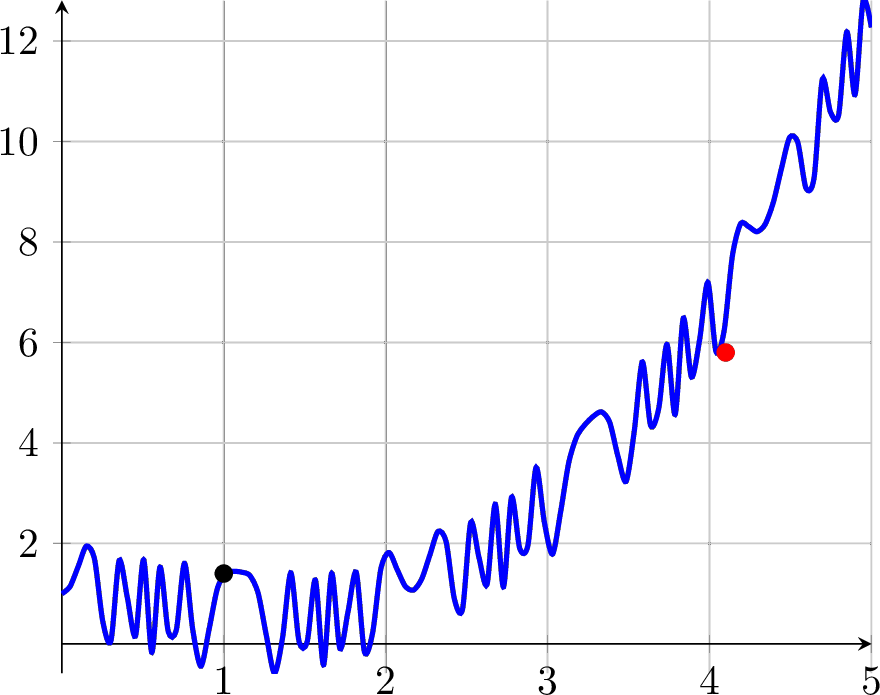
\includegraphics[width=0.5\linewidth]{images/Ch03_HardOptimization} 

}

\caption{A challenging numerical optimization problem. If we start at the black point then how will any of our algorithms find the local minimum at the red point?}\label{fig:num-opt-challenging}
\end{figure}

\begin{center}\rule{0.5\linewidth}{0.5pt}\end{center}

\hypertarget{multivariable-optimization}{%
\subsection{Multivariable Optimization}\label{multivariable-optimization}}

Now let's look at multivariable optimization. The analytic process for
finding optimal solutions is essentially the same as for single
variable.

\begin{itemize}
\item
  Write a function that models a scenario in multiple variables,
\item
  find the gradient vector (presuming that the function is
  differentiable),
\item
  set the gradient vector equal to the zero vector and solve for the
  critical point(s), and
\item
  interpret your answer in the context of the problem.
\end{itemize}

The trouble with unconstrained multivariable optimization is that
finding the critical points is now equivalent to solving a system of
nonlinear equations; a task that is likely impossible even with a
computer algebra system.

Let's see if you can extend your intuition from single variable to
multivariable. This particular subsection is intentionally quite brief. If you want more details on multivariable optimization it would be wise to take a full course in optimization.

\begin{center}\rule{0.5\linewidth}{0.5pt}\end{center}

\begin{exercise}
\protect\hypertarget{exr:unnamed-chunk-203}{}{\label{exr:unnamed-chunk-203} }The derivative free optimization method discussed in the single variable
optimization section just said that you should pick two points and pick
the one that takes you furthest uphill.

\begin{enumerate}
\def\labelenumi{\alph{enumi}.}
\item
  Why is it insufficient to choose just two points if we are dealing
  with a function of two variables? Hint: think about contour line.
\item
  For a function of two variables, how many points should you use to
  compare and determine the direction of ``uphill''?
\item
  Extend your answer from part (b) to \(n\) dimensions. How many points
  should we compare if we are in \(n\) dimensions and need to determine
  which direction is ``uphill''?
\item
  Back in the case of a two-variable function, you should have decided
  that three points was best. Explain an algorithm for moving one
  point at a time so that your three points eventually converge to a
  nearby local maximum. It may be helpful to make a surface plot or a
  contour plot of a well-known function just as a visual.
\end{enumerate}
\end{exercise}

\begin{center}\rule{0.5\linewidth}{0.5pt}\end{center}

\begin{exercise}
\protect\hypertarget{exr:unnamed-chunk-204}{}{\label{exr:unnamed-chunk-204} }Now let's tackle the gradient ascent/descent algorithm. You should
recall that the gradient vector points in the direction of maximum
change. How can you use this fact to modify the gradient ascent/descent
algorithm given previously? Clearly write your algorithm so that a
classmate could turn it into code.
\end{exercise}

\begin{center}\rule{0.5\linewidth}{0.5pt}\end{center}

\begin{exercise}
\protect\hypertarget{exr:unnamed-chunk-205}{}{\label{exr:unnamed-chunk-205} }How does the Monte Carlo algorithm extend to a two-variable optimization
problem? Clearly write your algorithm.
\end{exercise}

\begin{center}\rule{0.5\linewidth}{0.5pt}\end{center}

\begin{exercise}
\protect\hypertarget{exr:unnamed-chunk-206}{}{\label{exr:unnamed-chunk-206} }Try out the three algorithms that you just wrote on the function
\(f(x,y) =  \sin(x)\cos(y) + 0.1 x^2\) which has many local extrema and no global
maximum.
\end{exercise}

\begin{center}\rule{0.5\linewidth}{0.5pt}\end{center}

\begin{exercise}
\protect\hypertarget{exr:unnamed-chunk-207}{}{\label{exr:unnamed-chunk-207} }The derivative free, gradient ascent/descent, and monte carlo techniques
still have good analogues in higher dimensions. We just need to be a bit
careful since in higher dimensions there is much more room to move.
Below we'll give the full description of the gradient ascent/descent
algorithm. We don't give the full description of the derivative free or
Monte Carlo algorithms since there are many ways to implement them. The
interested reader should see a course in mathematical optimization or
machine learning.
\end{exercise}

\begin{center}\rule{0.5\linewidth}{0.5pt}\end{center}

\begin{definition}[The Gradient Descent Algorithm]
\protect\hypertarget{def:unnamed-chunk-208}{}{\label{def:unnamed-chunk-208} \iffalse (The Gradient Descent Algorithm) \fi{} }We want to solve the problem
\[\text{minimize } f(x_1, x_2, \ldots, x_n) \text{ subject to }(x_1, x_2, \ldots, x_n) \in S.\]

\begin{enumerate}
\def\labelenumi{\alph{enumi}.}
\item
  Choose an arbitrary starting point
  \(\boldsymbol{x}_0 = (x_1,x_2,\ldots,x_n)\in S\).
\item
  We are going to define a difference equation that gives successive
  guesses for the optimal value:
  \[\boldsymbol{x}_{n+1} = \boldsymbol{x}_n - \alpha \nabla f(\boldsymbol{x}_n).\] The difference
  equation says to follow the negative gradient a certain distance
  from your present point (why are we doing this). Note that the value
  of \(\alpha\) is up to you so experiment with a few values (you should
  probably take \(\alpha \le 1\) \ldots why?).
\item
  Repeat the iterative process in step b until two successive points
  are \emph{close enough} to each other.
\end{enumerate}
\end{definition}

\begin{center}\rule{0.5\linewidth}{0.5pt}\end{center}

Take Note: If you are looking to maximize your objective function then in the
Monte-Carlo search you should examine if \(z\) is greater than your
current largest value. For gradient descent you should actually do a
gradient \emph{ascent} and follow the positive gradient instead of the
negative gradient.

\begin{center}\rule{0.5\linewidth}{0.5pt}\end{center}

\begin{exercise}
\protect\hypertarget{exr:unnamed-chunk-209}{}{\label{exr:unnamed-chunk-209} }Write generic code to implement the Gradient Descent algorithm in as
many dimensions as necessary and test your code on a multivariable
function where you know the location and value of a local minimum.
\end{exercise}

\begin{center}\rule{0.5\linewidth}{0.5pt}\end{center}

\begin{exercise}
\protect\hypertarget{exr:unnamed-chunk-210}{}{\label{exr:unnamed-chunk-210} }The functions like \(f(x,y) = \sin(x)\cos(y)\) have many local extreme
values which makes optimization challenging. Impelement your Gradient
Descent code on this function to find the local minimum \((0,0)\). Start
somewhere near \((0,0)\) and show by way of example that your gradient
descent code may not converge to this particular local minimum. Why is
this important?
\end{exercise}

\begin{center}\rule{0.5\linewidth}{0.5pt}\end{center}

\hypertarget{calculus-with-numpy-and-scipy}{%
\section{\texorpdfstring{Calculus with \texttt{numpy} and \texttt{scipy}}{Calculus with numpy and scipy}}\label{calculus-with-numpy-and-scipy}}

In this section we will look at some highly versatile functions built into the \texttt{numpy} and \texttt{scipy} libraries in Python. These libraries allow us to lean on pre-built numerical routines for calculus and optimization and instead we can focus our energies on setting up the problems and interpreting solutions. The down side here is that we are going to treat some of the optimization routines in Python as black boxes, so part of the goal of this section is to partially unpack these black boxes so that we know what's going on under the hood. If you haven't done Exercise \ref{exr:fsolve} yet you may want to do so now in order to get used to some of the syntax used by the Python \texttt{scipy} library.

\hypertarget{differentiation-1}{%
\subsection{Differentiation}\label{differentiation-1}}

There are two main tools built into the \texttt{numpy} and \texttt{scipy} libraries that do numerical differentiation. In \texttt{numpy} there is the \texttt{np.diff()} command. In \texttt{scipy} there is the \texttt{scipy.misc.derivative()} command.

\begin{center}\rule{0.5\linewidth}{0.5pt}\end{center}

\begin{exercise}
\protect\hypertarget{exr:unnamed-chunk-211}{}{\label{exr:unnamed-chunk-211} }In the following blocks of Python code we demonstrate what the \texttt{np.diff()} command does. Use these examples to give a thorough description for what \texttt{np.diff()} does to a Python list.
\end{exercise}

\textbf{First example of \texttt{np.diff()}:}

\begin{Shaded}
\begin{Highlighting}[]
\ImportTok{import}\NormalTok{ numpy }\ImportTok{as}\NormalTok{ np}
\NormalTok{myList }\OperatorTok{=}\NormalTok{ np.arange(}\DecValTok{0}\NormalTok{,}\DecValTok{10}\NormalTok{)}
\BuiltInTok{print}\NormalTok{(myList)}
\end{Highlighting}
\end{Shaded}

\begin{verbatim}
## [0 1 2 3 4 5 6 7 8 9]
\end{verbatim}

\begin{Shaded}
\begin{Highlighting}[]
\BuiltInTok{print}\NormalTok{( np.diff(myList) )}
\end{Highlighting}
\end{Shaded}

\begin{verbatim}
## [1 1 1 1 1 1 1 1 1]
\end{verbatim}

\textbf{Second example of \texttt{np.diff()}:}

\begin{Shaded}
\begin{Highlighting}[]
\ImportTok{import}\NormalTok{ numpy }\ImportTok{as}\NormalTok{ np}
\NormalTok{myList }\OperatorTok{=}\NormalTok{ np.linspace(}\DecValTok{0}\NormalTok{,}\DecValTok{1}\NormalTok{,}\DecValTok{6}\NormalTok{)}
\BuiltInTok{print}\NormalTok{(myList)}
\end{Highlighting}
\end{Shaded}

\begin{verbatim}
## [0.  0.2 0.4 0.6 0.8 1. ]
\end{verbatim}

\begin{Shaded}
\begin{Highlighting}[]
\BuiltInTok{print}\NormalTok{( np.diff(myList) )}
\end{Highlighting}
\end{Shaded}

\begin{verbatim}
## [0.2 0.2 0.2 0.2 0.2]
\end{verbatim}

\textbf{Third example of \texttt{np.diff()}:}

\begin{Shaded}
\begin{Highlighting}[]
\ImportTok{import}\NormalTok{ numpy }\ImportTok{as}\NormalTok{ np}
\NormalTok{x }\OperatorTok{=}\NormalTok{ np.linspace(}\DecValTok{0}\NormalTok{,}\DecValTok{1}\NormalTok{,}\DecValTok{6}\NormalTok{)}
\NormalTok{dx }\OperatorTok{=}\NormalTok{ x[}\DecValTok{1}\NormalTok{]}\OperatorTok{{-}}\NormalTok{x[}\DecValTok{0}\NormalTok{]}
\NormalTok{y }\OperatorTok{=}\NormalTok{ x}\OperatorTok{**}\DecValTok{2}
\NormalTok{dy }\OperatorTok{=} \DecValTok{2}\OperatorTok{*}\NormalTok{x}
\BuiltInTok{print}\NormalTok{(}\StringTok{"function values: }\CharTok{\textbackslash{}n}\StringTok{"}\NormalTok{,y)}
\end{Highlighting}
\end{Shaded}

\begin{verbatim}
## function values: 
##  [0.   0.04 0.16 0.36 0.64 1.  ]
\end{verbatim}

\begin{Shaded}
\begin{Highlighting}[]
\BuiltInTok{print}\NormalTok{(}\StringTok{"exact values of derivative: }\CharTok{\textbackslash{}n}\StringTok{"}\NormalTok{,dy)}
\end{Highlighting}
\end{Shaded}

\begin{verbatim}
## exact values of derivative: 
##  [0.  0.4 0.8 1.2 1.6 2. ]
\end{verbatim}

\begin{Shaded}
\begin{Highlighting}[]
\BuiltInTok{print}\NormalTok{(}\StringTok{"values from np.diff(): }\CharTok{\textbackslash{}n}\StringTok{"}\NormalTok{,np.diff(y))}
\end{Highlighting}
\end{Shaded}

\begin{verbatim}
## values from np.diff(): 
##  [0.04 0.12 0.2  0.28 0.36]
\end{verbatim}

\begin{Shaded}
\begin{Highlighting}[]
\BuiltInTok{print}\NormalTok{(}\StringTok{"values from np.diff()/dx: }\CharTok{\textbackslash{}n}\StringTok{"}\NormalTok{,np.diff(y) }\OperatorTok{/}\NormalTok{ dx )}
\end{Highlighting}
\end{Shaded}

\begin{verbatim}
## values from np.diff()/dx: 
##  [0.2 0.6 1.  1.4 1.8]
\end{verbatim}

\begin{center}\rule{0.5\linewidth}{0.5pt}\end{center}

\begin{exercise}
\protect\hypertarget{exr:unnamed-chunk-215}{}{\label{exr:unnamed-chunk-215} }Why does the \texttt{np.diff()} command produce a list that is one element shorter than the original list?
\end{exercise}

\begin{center}\rule{0.5\linewidth}{0.5pt}\end{center}

\begin{exercise}
\protect\hypertarget{exr:unnamed-chunk-216}{}{\label{exr:unnamed-chunk-216} }If we have a list of \(x\) values and a list of \(y\) values for a function \(y=f(x)\) then how do we use \texttt{np.diff()} to approximate the first derivative of \(f(x)\)? What is the order of the error in the approximation?
\end{exercise}

\begin{center}\rule{0.5\linewidth}{0.5pt}\end{center}

\begin{exercise}
\protect\hypertarget{exr:unnamed-chunk-217}{}{\label{exr:unnamed-chunk-217} }What does the following block of Python code do?
\end{exercise}

\begin{Shaded}
\begin{Highlighting}[]
\ImportTok{import}\NormalTok{ numpy }\ImportTok{as}\NormalTok{ np}
\NormalTok{x }\OperatorTok{=}\NormalTok{ np.linspace(}\DecValTok{0}\NormalTok{,}\DecValTok{1}\NormalTok{,}\DecValTok{6}\NormalTok{)}
\NormalTok{dx }\OperatorTok{=}\NormalTok{ x[}\DecValTok{1}\NormalTok{]}\OperatorTok{{-}}\NormalTok{x[}\DecValTok{0}\NormalTok{]}
\NormalTok{y }\OperatorTok{=}\NormalTok{ x}\OperatorTok{**}\DecValTok{2}
\BuiltInTok{print}\NormalTok{( np.diff(y,}\DecValTok{2}\NormalTok{) }\OperatorTok{/}\NormalTok{ dx}\OperatorTok{**}\DecValTok{2}\NormalTok{ )}
\end{Highlighting}
\end{Shaded}

\begin{verbatim}
## [2. 2. 2. 2.]
\end{verbatim}

\begin{center}\rule{0.5\linewidth}{0.5pt}\end{center}

\begin{exercise}
\protect\hypertarget{exr:unnamed-chunk-219}{}{\label{exr:unnamed-chunk-219} }Use the \texttt{np.diff()} command to approximate the first and second derivatives of the function \(f(x) = x\sin(x) - \ln(x)\) on the domain \([1,5]\). Then create a plot that shows \(f(x)\) and the approximations of \(f'(x)\) and \(f''(x)\).
\end{exercise}

\begin{center}\rule{0.5\linewidth}{0.5pt}\end{center}

\begin{exercise}
\protect\hypertarget{exr:unnamed-chunk-220}{}{\label{exr:unnamed-chunk-220} }Next we look into the \texttt{scipy.misc.derivative()} command from the \texttt{scipy} library. This will be another way to calculate the derivative of a function. One advantage will be that you can just send in a Python function (or a lambda function) without actually computing the lists of values. Examine the following Python code and fully describe what it does.
\end{exercise}

\begin{Shaded}
\begin{Highlighting}[]
\ImportTok{import}\NormalTok{ numpy }\ImportTok{as}\NormalTok{ np}
\ImportTok{import}\NormalTok{ scipy.misc}
\NormalTok{f }\OperatorTok{=} \KeywordTok{lambda}\NormalTok{ x: x}\OperatorTok{**}\DecValTok{2}
\NormalTok{x }\OperatorTok{=}\NormalTok{ np.linspace(}\DecValTok{1}\NormalTok{,}\DecValTok{5}\NormalTok{,}\DecValTok{5}\NormalTok{)}
\NormalTok{df }\OperatorTok{=}\NormalTok{ scipy.misc.derivative(f,x,dx }\OperatorTok{=} \FloatTok{1e{-}10}\NormalTok{)}
\BuiltInTok{print}\NormalTok{(df)}
\end{Highlighting}
\end{Shaded}

\begin{verbatim}
## [ 2.00000017  4.00000033  6.0000005   8.00000066 10.00000083]
\end{verbatim}

One advantage to using \texttt{scipy.misc.derivative()} is that you get to dictate the error in the derivative computation, and that error is not tied to the list of values that you provide. In its simplest form you can provide just a single \(x\) value just like in the next block of code.

\begin{Shaded}
\begin{Highlighting}[]
\ImportTok{import}\NormalTok{ numpy }\ImportTok{as}\NormalTok{ np}
\ImportTok{import}\NormalTok{ scipy.misc}
\NormalTok{f }\OperatorTok{=} \KeywordTok{lambda}\NormalTok{ x: x}\OperatorTok{**}\DecValTok{2}
\NormalTok{df }\OperatorTok{=}\NormalTok{ scipy.misc.derivative(f,}\DecValTok{1}\NormalTok{,dx }\OperatorTok{=} \FloatTok{1e{-}10}\NormalTok{) }\CommentTok{\# derivative at x=1}
\BuiltInTok{print}\NormalTok{(df)}
\end{Highlighting}
\end{Shaded}

\begin{verbatim}
## 2.000000165480742
\end{verbatim}

\begin{center}\rule{0.5\linewidth}{0.5pt}\end{center}

\begin{exercise}
\protect\hypertarget{exr:unnamed-chunk-223}{}{\label{exr:unnamed-chunk-223} }In the following code we find the first and second derivatives of \(f(x) = x\sin(x) - \ln(x)\) using \texttt{scipy.misc.derivative()}. Notice that we've chosen to take \texttt{dx=1e-6} for each of the derivative computations. That may seem like an odd choice, but there is more going on here. Try successively smaller and smaller values for the \texttt{dx} parameter. What do you find? Why does it happen?
\end{exercise}

\begin{Shaded}
\begin{Highlighting}[]
\ImportTok{import}\NormalTok{ numpy }\ImportTok{as}\NormalTok{ np}
\ImportTok{import}\NormalTok{ scipy.misc }
\ImportTok{import}\NormalTok{ matplotlib.pyplot }\ImportTok{as}\NormalTok{ plt}
\NormalTok{f }\OperatorTok{=} \KeywordTok{lambda}\NormalTok{ x: np.sin(x)}\OperatorTok{*}\NormalTok{x}\OperatorTok{{-}}\NormalTok{np.log(x)}
\NormalTok{x }\OperatorTok{=}\NormalTok{ np.linspace(}\DecValTok{1}\NormalTok{,}\DecValTok{5}\NormalTok{,}\DecValTok{100}\NormalTok{) }\CommentTok{\# x domain: 100 points between 1 and 5}
\NormalTok{df }\OperatorTok{=}\NormalTok{ scipy.misc.derivative(f,x,dx}\OperatorTok{=}\FloatTok{1e{-}6}\NormalTok{)}
\NormalTok{df2 }\OperatorTok{=}\NormalTok{ scipy.misc.derivative(f,x,dx}\OperatorTok{=}\FloatTok{1e{-}6}\NormalTok{,n}\OperatorTok{=}\DecValTok{2}\NormalTok{)}
\NormalTok{plt.plot(x,f(x),}\StringTok{\textquotesingle{}b\textquotesingle{}}\NormalTok{,x,df,}\StringTok{\textquotesingle{}r{-}{-}\textquotesingle{}}\NormalTok{,x,df2,}\StringTok{\textquotesingle{}k{-}{-}\textquotesingle{}}\NormalTok{)}
\NormalTok{plt.legend([}\StringTok{"f(x)"}\NormalTok{,}\StringTok{"f\textquotesingle{}(x)"}\NormalTok{,}\StringTok{"f\textquotesingle{}\textquotesingle{}(x)"}\NormalTok{])}
\NormalTok{plt.grid()}
\NormalTok{plt.show()}
\end{Highlighting}
\end{Shaded}

\begin{figure}

{\centering 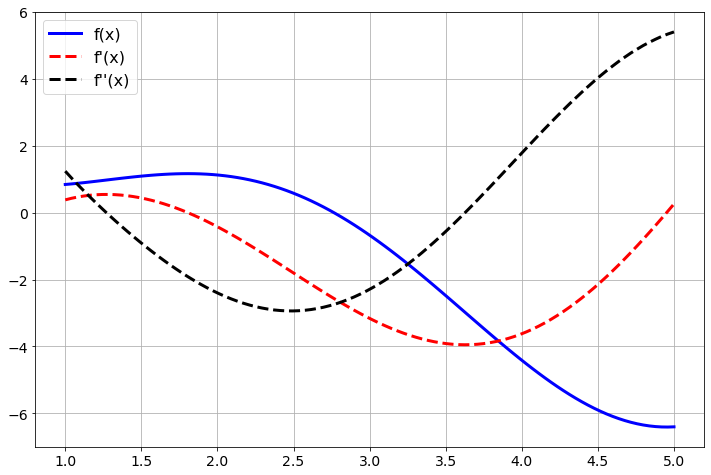
\includegraphics[width=0.75\linewidth]{images/Ch03_ScipyDerivatives} 

}

\caption{Derivatives with scipy}\label{fig:unnamed-chunk-225}
\end{figure}

\begin{center}\rule{0.5\linewidth}{0.5pt}\end{center}

\hypertarget{integration-1}{%
\subsection{Integration}\label{integration-1}}

In \texttt{numpy} there is a nice tool called \texttt{np.trapz()} that implements the trapezoidal rule. In the following problem you will find several examples of the \texttt{np.trapz()} command. Use these examples to determine how the command works to integrate functions.

\begin{center}\rule{0.5\linewidth}{0.5pt}\end{center}

\begin{exercise}
\protect\hypertarget{exr:unnamed-chunk-226}{}{\label{exr:unnamed-chunk-226} }First we'll approximate the integral \(\int_{-2}^2 x^2 dx\). The exact answer is
\[ \int_{-2}^2 x^2 dx = \frac{x^3}{3} \Big|_{-2}^2 = \frac{16}{3} = 5.3333... \]
\end{exercise}

\begin{Shaded}
\begin{Highlighting}[]
\ImportTok{import}\NormalTok{ numpy }\ImportTok{as}\NormalTok{ np}
\NormalTok{x }\OperatorTok{=}\NormalTok{ np.linspace(}\OperatorTok{{-}}\DecValTok{2}\NormalTok{,}\DecValTok{2}\NormalTok{,}\DecValTok{100}\NormalTok{)}
\NormalTok{dx }\OperatorTok{=}\NormalTok{ x[}\DecValTok{1}\NormalTok{]}\OperatorTok{{-}}\NormalTok{x[}\DecValTok{0}\NormalTok{]}
\NormalTok{y }\OperatorTok{=}\NormalTok{ x}\OperatorTok{**}\DecValTok{2}
\BuiltInTok{print}\NormalTok{(}\StringTok{"Approximate integral is "}\NormalTok{,np.trapz(y)}\OperatorTok{*}\NormalTok{dx)}
\end{Highlighting}
\end{Shaded}

\begin{verbatim}
## Approximate integral is  5.334421657653986
\end{verbatim}

Next we'll approximate \(\int_0^{2\pi} \sin(x) dx\). We know that the exact value is 0.

\begin{Shaded}
\begin{Highlighting}[]
\ImportTok{import}\NormalTok{ numpy }\ImportTok{as}\NormalTok{ np}
\NormalTok{x }\OperatorTok{=}\NormalTok{ np.linspace(}\DecValTok{0}\NormalTok{,}\DecValTok{2}\OperatorTok{*}\NormalTok{np.pi,}\DecValTok{100}\NormalTok{)}
\NormalTok{dx }\OperatorTok{=}\NormalTok{ x[}\DecValTok{1}\NormalTok{]}\OperatorTok{{-}}\NormalTok{x[}\DecValTok{0}\NormalTok{]}
\NormalTok{y }\OperatorTok{=}\NormalTok{ np.sin(x)}
\BuiltInTok{print}\NormalTok{(}\StringTok{"Approximate integral is "}\NormalTok{,np.trapz(y)}\OperatorTok{*}\NormalTok{dx)}
\end{Highlighting}
\end{Shaded}

\begin{verbatim}
## Approximate integral is  -2.2019371830862577e-17
\end{verbatim}

Pick a function and an interval for which you know the exact definite integral. Demonstrate how to use \texttt{np.trapz()} on your definite integral.

\begin{center}\rule{0.5\linewidth}{0.5pt}\end{center}

\begin{exercise}
\protect\hypertarget{exr:unnamed-chunk-229}{}{\label{exr:unnamed-chunk-229} }Notice in the last examples that we multiplied the result of the \texttt{np.trapz()} command by \texttt{dx}. Why did we do this? What is the \texttt{np.trapz()} command doing without the \texttt{dx}?
\end{exercise}

\begin{center}\rule{0.5\linewidth}{0.5pt}\end{center}

In the \texttt{scipy} library there is a more general tool called \texttt{scipy.integrate.quad()}. The term ``quad'' is short for ``quadrature''. In numerical analysis literature rules like Simpson's rule are called quadrature rules for integration. The function \texttt{scipy.integrate.quad()} accepts a Python function (or a lambda function) and the bounds of the definite integral. It outputs an approximation of the integral along with an approximation of the error in the integral calculation. See the Python code below.

\begin{Shaded}
\begin{Highlighting}[]
\ImportTok{import}\NormalTok{ numpy }\ImportTok{as}\NormalTok{ np}
\ImportTok{import}\NormalTok{ scipy.integrate}
\NormalTok{f }\OperatorTok{=} \KeywordTok{lambda}\NormalTok{ x: x}\OperatorTok{**}\DecValTok{2}
\NormalTok{I }\OperatorTok{=}\NormalTok{ scipy.integrate.quad(f,}\OperatorTok{{-}}\DecValTok{2}\NormalTok{,}\DecValTok{2}\NormalTok{)}
\BuiltInTok{print}\NormalTok{(I)}
\end{Highlighting}
\end{Shaded}

\begin{verbatim}
## (5.333333333333333, 5.921189464667501e-14)
\end{verbatim}

\begin{center}\rule{0.5\linewidth}{0.5pt}\end{center}

\begin{exercise}
\protect\hypertarget{exr:unnamed-chunk-231}{}{\label{exr:unnamed-chunk-231} }What are the advantages and disadvantages to using the \texttt{scipy.integrate.quad()} command as compared to the \texttt{np.trapz()} command.
\end{exercise}

\begin{center}\rule{0.5\linewidth}{0.5pt}\end{center}

\begin{exercise}
\protect\hypertarget{exr:unnamed-chunk-232}{}{\label{exr:unnamed-chunk-232} }If you have data for the hourly rate at which water is being drained from a dam and you want to find the total amount of water drained over the course of the time in the dataset, then which of the tools that we know would you use? Why?
\end{exercise}

\begin{center}\rule{0.5\linewidth}{0.5pt}\end{center}

\hypertarget{optimization-1}{%
\subsection{Optimization}\label{optimization-1}}

As you've seen in this section there are many tools built into \texttt{numpy} and \texttt{scipy} that will do some of our basic numerical computations. The same is true for numerical optimization problems. Keep in mind throughout the remainder of this section that the whole topic of numerical optimization is still an active area of research and there is much more to the story that what we'll see here. However, the Python tools that we will use are highly optimized and tend to work quite well.

\begin{center}\rule{0.5\linewidth}{0.5pt}\end{center}

\begin{exercise}
\protect\hypertarget{exr:unnamed-chunk-233}{}{\label{exr:unnamed-chunk-233} }Let's solve a very simple function minimization problem to get started. Consider the function \(f(x) = (x-3)^2 - 5\). A moment's thought reveals that the global minimum of this parabolic function occurs at \((3,-5)\). We can have \texttt{scipy.optimize.minimize()} find this value for us numerically. The routine is much like Newton's Method in that we give it a starting point \emph{near} where we think the optimum will be and it will iterate through some algorithm (like a derivative free optimization routine) to approximate the minimum.
\end{exercise}

\begin{Shaded}
\begin{Highlighting}[]
\ImportTok{import}\NormalTok{ numpy }\ImportTok{as}\NormalTok{ np}
\ImportTok{from}\NormalTok{ scipy.optimize }\ImportTok{import}\NormalTok{ minimize}
\NormalTok{f }\OperatorTok{=} \KeywordTok{lambda}\NormalTok{ x: (x}\OperatorTok{{-}}\DecValTok{3}\NormalTok{)}\OperatorTok{**}\DecValTok{2} \OperatorTok{{-}} \DecValTok{5}
\NormalTok{minimize(f,}\DecValTok{2}\NormalTok{)}
\end{Highlighting}
\end{Shaded}

\begin{verbatim}
##       fun: -5.0
##  hess_inv: array([[0.49999999]])
##       jac: array([0.])
##   message: 'Optimization terminated successfully.'
##      nfev: 9
##       nit: 2
##      njev: 3
##    status: 0
##   success: True
##         x: array([2.99999998])
\end{verbatim}

\begin{enumerate}
\def\labelenumi{\alph{enumi}.}
\tightlist
\item
  Implement the code above then spend some time playing around with the minimize command to minimize more challenging functions.
\item
  Explain what all of the output information is from the \texttt{.minimize()} command.
\end{enumerate}

\begin{center}\rule{0.5\linewidth}{0.5pt}\end{center}

\begin{exercise}
\protect\hypertarget{exr:unnamed-chunk-235}{}{\label{exr:unnamed-chunk-235} }There is not a function called \texttt{scipy.optimize.maximize()}. Instead, Python expects you to rewrite every maximization problem as a minimization problem. How do you do that?
\end{exercise}

\begin{center}\rule{0.5\linewidth}{0.5pt}\end{center}

\begin{exercise}
\protect\hypertarget{exr:unnamed-chunk-236}{}{\label{exr:unnamed-chunk-236} }Solve Exercise \ref{exr:cardboard-problem} using \texttt{scipy.optimize.minimize()}.
\end{exercise}

\begin{center}\rule{0.5\linewidth}{0.5pt}\end{center}

\hypertarget{least-squares-curve-fitting}{%
\section{Least Squares Curve Fitting}\label{least-squares-curve-fitting}}

In this section we'll change our focus a bit to look at a different question from algebra, and, in turn, reveal a hidden numerical optimization problem where the \texttt{scipy.optimize.minimize()} tool will come in quite handy.

Here is the primary question of interest:\\
\emph{If we have a few data points and a reasonable guess for the type of function fitting the points, how would we determine the actual function?}

You may recognize this as the basic question of regression from statistics. What we will do here is pose the statistical question of which curve best fits a data set as an optimization problem. Then we will use the tools that we've built so far to solve the optimization problem.

\begin{center}\rule{0.5\linewidth}{0.5pt}\end{center}

\begin{exercise}
\protect\hypertarget{exr:unnamed-chunk-237}{}{\label{exr:unnamed-chunk-237} }Consider the function \(f(x)\) that goes exactly through the points
\((0,1)\), \((1,4)\), and \((2,13)\).

\begin{enumerate}
\def\labelenumi{\alph{enumi}.}
\item
  Find a function that goes through these points exactly. Be able to
  defend your work.
\item
  Is your function unique? That is to say, is there another function
  out there that also goes exactly through these points?
\end{enumerate}
\end{exercise}

\begin{center}\rule{0.5\linewidth}{0.5pt}\end{center}

\begin{exercise}
\protect\hypertarget{exr:first-least-squares}{}{\label{exr:first-least-squares} }Now let's make a minor tweak to the previous problem. Let's say that we
have the data points \((0,1.07)\), \((1,3.9)\), \((2,14.8)\), and \((3,26.8)\).
Notice that these points are \emph{close} to the points we had in the
previous problem, but all of the \(y\) values have a little noise in them
and we have added a fourth point. If we suspect that a function \(f(x)\)
that \emph{best} fits this data is quadratic then \(f(x) = ax^2 +  bx + c\) for some constants \(a\), \(b\), and \(c\).

\begin{enumerate}
\def\labelenumi{\alph{enumi}.}
\item
  Plot the four points along with the function \(f(x)\) for arbitrarily
  chosen values of \(a\), \(b\), and \(c\).
\item
  Work with your partner(s) to systematically change \(a\), \(b\), and \(c\) so that you get a good visual match to the data. The Python code below will help you get started.
\end{enumerate}
\end{exercise}

\begin{Shaded}
\begin{Highlighting}[]
\ImportTok{import}\NormalTok{ numpy }\ImportTok{as}\NormalTok{ np}
\ImportTok{import}\NormalTok{ matplotlib.pyplot }\ImportTok{as}\NormalTok{ plt}
\NormalTok{xdata }\OperatorTok{=}\NormalTok{ np.array([}\DecValTok{0}\NormalTok{, }\DecValTok{1}\NormalTok{, }\DecValTok{2}\NormalTok{, }\DecValTok{3}\NormalTok{])}
\NormalTok{ydata }\OperatorTok{=}\NormalTok{ np.array([}\FloatTok{1.07}\NormalTok{, }\FloatTok{3.9}\NormalTok{, }\FloatTok{14.8}\NormalTok{, }\FloatTok{26.8}\NormalTok{])}
\NormalTok{a }\OperatorTok{=} \DecValTok{1}
\NormalTok{b }\OperatorTok{=} \DecValTok{1}
\NormalTok{c }\OperatorTok{=} \DecValTok{1}
\NormalTok{x }\OperatorTok{=}\NormalTok{ np.linspace(}\DecValTok{0}\NormalTok{,}\DecValTok{4}\NormalTok{,}\DecValTok{100}\NormalTok{)}
\NormalTok{guess }\OperatorTok{=}\NormalTok{ a}\OperatorTok{*}\NormalTok{x}\OperatorTok{**}\DecValTok{2} \OperatorTok{+}\NormalTok{ b}\OperatorTok{*}\NormalTok{x }\OperatorTok{+}\NormalTok{ c}
\NormalTok{plt.plot(xdata,ydata,}\StringTok{\textquotesingle{}bo\textquotesingle{}}\NormalTok{,markersize}\OperatorTok{=}\DecValTok{5}\NormalTok{)}
\NormalTok{plt.plot(x,guess,}\StringTok{\textquotesingle{}r{-}{-}\textquotesingle{}}\NormalTok{)}
\NormalTok{plt.grid()}
\NormalTok{plt.legend([}\StringTok{\textquotesingle{}Data\textquotesingle{}}\NormalTok{,}\StringTok{\textquotesingle{}Guess\textquotesingle{}}\NormalTok{])}
\NormalTok{plt.show()}
\end{Highlighting}
\end{Shaded}

\begin{figure}

{\centering 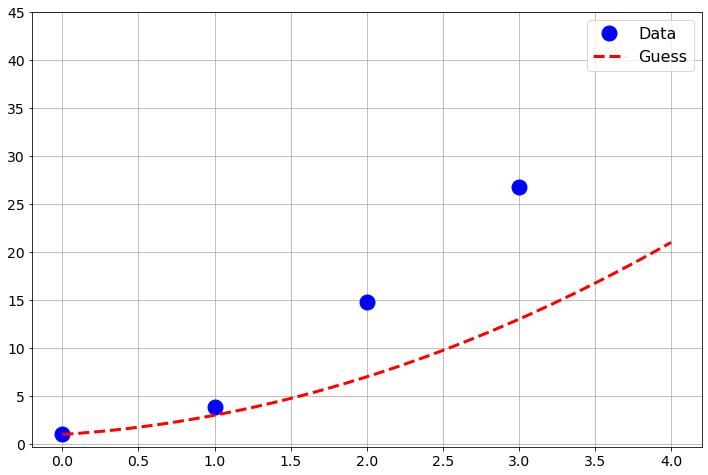
\includegraphics[width=0.75\linewidth]{images/Ch03_DataMatch} 

}

\caption{Initial attempt at matching data with a quadratic.}\label{fig:unnamed-chunk-239}
\end{figure}

\begin{center}\rule{0.5\linewidth}{0.5pt}\end{center}

\begin{exercise}
\protect\hypertarget{exr:unnamed-chunk-240}{}{\label{exr:unnamed-chunk-240} }Now let's be a bit more systematic about things from the previous problem. Let's say that you have a pretty good guess that \(b \approx 2\) and \(c \approx 0.7\). We need to get a good estimate for \(a\).

\begin{enumerate}
\def\labelenumi{\alph{enumi}.}
\tightlist
\item
  Pick an arbitrary starting value for \(a\) then for each of the four points find the error between the predicted \(y\) value and the actual \(y\) value. These errors are called the \emph{residuals}.
\item
  Square all four of your errors and add them up. (Pause, ponder, and discuss: why are we squaring the errors before we sum them?)
\item
  Now change your value of \(a\) to several different values and record the sum of the square errors for each of your values of \(a\). It may be worth while to use a spreadsheet to keep track of your work here.
\item
  Make a plot with the value of \(a\) on the horizontal axis and the value of the sum of the square errors on the vertical axis. Use your plot to defend the optimal choice for \(a\).
\end{enumerate}
\end{exercise}

\begin{center}\rule{0.5\linewidth}{0.5pt}\end{center}

\begin{exercise}
\protect\hypertarget{exr:unnamed-chunk-241}{}{\label{exr:unnamed-chunk-241} }We're going to revisit part (c) of the previous problem. Write a loop that tries many values of \(a\) in very small increments and calculates the sum of the squared errors. The following partial Python code should help you get started. In the resulting plot you should see a clear local minimum. What does that minimum tell you about solving this problem?
\end{exercise}

\begin{Shaded}
\begin{Highlighting}[]
\ImportTok{import}\NormalTok{ numpy }\ImportTok{as}\NormalTok{ np}
\ImportTok{import}\NormalTok{ matplotlib.pyplot }\ImportTok{as}\NormalTok{ plt}
\NormalTok{xdata }\OperatorTok{=}\NormalTok{ np.array([}\DecValTok{0}\NormalTok{, }\DecValTok{1}\NormalTok{, }\DecValTok{2}\NormalTok{, }\DecValTok{3}\NormalTok{])}
\NormalTok{ydata }\OperatorTok{=}\NormalTok{ np.array([}\FloatTok{1.07}\NormalTok{, }\FloatTok{3.9}\NormalTok{, }\FloatTok{14.8}\NormalTok{, }\FloatTok{26.8}\NormalTok{])}
\NormalTok{b }\OperatorTok{=} \DecValTok{2}
\NormalTok{c }\OperatorTok{=} \FloatTok{0.75}
\NormalTok{A }\OperatorTok{=} \CommentTok{\# give a numpy array of values for a}
\NormalTok{SumSqRes }\OperatorTok{=}\NormalTok{ [] }\CommentTok{\# this is blank storage for the sum of the squared residuals}
\ControlFlowTok{for}\NormalTok{ a }\KeywordTok{in}\NormalTok{ A:}
\NormalTok{  guess }\OperatorTok{=}\NormalTok{ a}\OperatorTok{*}\NormalTok{xdata}\OperatorTok{**}\DecValTok{2} \OperatorTok{+}\NormalTok{ b}\OperatorTok{*}\NormalTok{xdata }\OperatorTok{+}\NormalTok{ c}
\NormalTok{  residuals }\OperatorTok{=} \CommentTok{\# write code to calculate the residuals}
\NormalTok{  SumSqRes.append(  ) }\CommentTok{\# inside the parenthesis calculate the sum of the squared residuals}
\NormalTok{plt.plot(A,SumSqRes,}\StringTok{\textquotesingle{}r*\textquotesingle{}}\NormalTok{)}
\NormalTok{plt.grid()}
\NormalTok{plt.xlabel(}\StringTok{\textquotesingle{}Value of a\textquotesingle{}}\NormalTok{)}
\NormalTok{plt.ylabel(}\StringTok{\textquotesingle{}Sum of squared residuals\textquotesingle{}}\NormalTok{)}
\NormalTok{plt.show()}
\end{Highlighting}
\end{Shaded}

\begin{center}\rule{0.5\linewidth}{0.5pt}\end{center}

Now let's formalize the process that we've described in the previous problems.

\begin{definition}[Least Squares Regression]
\protect\hypertarget{def:least-squares}{}{\label{def:least-squares} \iffalse (Least Squares Regression) \fi{} }Let
\[S = \{ (x_1, y_1), \, (x_2, y_2), \, \ldots, \, (x_n, y_n) \}\] be a
set of \(n\) ordered pairs in \(\mathbb{R}^2\). If we guess that a function
\(f(x)\) is a best choice to fit the data and if \(f(x)\) depends on
parameters \(a_1, a_2, \ldots, a_n\) then

\begin{enumerate}
\def\labelenumi{\alph{enumi}.}
\item
  Pick initial values for the parameters \(a_1, a_2, \ldots, a_n\) so that
  the function \(f(x)\) \emph{looks like} it is close to the data (this is
  strictly a visual step \ldots take care that it may take some playing
  around to guess the initial values of the parameters)
\item
  Calculate the square error between the data point and the prediction
  from the function \(f(x)\)
  \[\text{error for the point $x_i$: } e_i = \left( y_i - f(x_i) \right)^2.\]
  Note that squaring the error has the advantages of removing the
  sign, accentuating errors larger than 1, and decreasing errors that
  are less than 1.
\item
  As a measure of the total error between the function and the data,
  sum the squared errors
  \[\text{sum of square errors } = \sum_{i=1}^n \left( y_i - f(x_i) \right)^2.\]
  (Take note that if there were a continuum of points instead of a
  discrete set then we would integrate the square errors instead of
  taking a sum.)
\item
  Change the parameters \(a_1, a_2, \ldots\) so as to minimize the sum
  of the square errors.
\end{enumerate}
\end{definition}

\begin{center}\rule{0.5\linewidth}{0.5pt}\end{center}

\begin{exercise}
\protect\hypertarget{exr:unnamed-chunk-243}{}{\label{exr:unnamed-chunk-243} }In \ref{def:least-squares} the last step is a bit vague. That was purposeful since there are many techniques that could be used to minimize the sum of the square errors. However, if we just think about the sum of the squared residuals as a function then we can apply \texttt{scipy.optimize.minimize()} to that function in order to return the values of the parameters that best minimize the sum of the squared residuals. The following blocks of Python code implement the idea in a very streamlined way. Go through the code and comment each line to describe exactly what it does.
\end{exercise}

\begin{Shaded}
\begin{Highlighting}[]
\ImportTok{import}\NormalTok{ numpy }\ImportTok{as}\NormalTok{ np}
\ImportTok{import}\NormalTok{ matplotlib.pyplot }\ImportTok{as}\NormalTok{ plt}
\ImportTok{from}\NormalTok{ scipy.optimize }\ImportTok{import}\NormalTok{ minimize}

\NormalTok{xdata }\OperatorTok{=}\NormalTok{ np.array([}\DecValTok{0}\NormalTok{, }\DecValTok{1}\NormalTok{, }\DecValTok{2}\NormalTok{, }\DecValTok{3}\NormalTok{])}
\NormalTok{ydata }\OperatorTok{=}\NormalTok{ np.array([}\FloatTok{1.07}\NormalTok{, }\FloatTok{3.9}\NormalTok{, }\FloatTok{14.8}\NormalTok{, }\FloatTok{26.8}\NormalTok{])}

\KeywordTok{def}\NormalTok{ SSRes(parameters):}
  \CommentTok{\# In the next line of code we want to build our quadratic approximation.}
  \CommentTok{\# y = ax\^{}2 + bx + c}
  \CommentTok{\# We are sending in a list of parameters so }
  \CommentTok{\# a = parameters[0], b = parameters[1], and c = parameters[2]}
\NormalTok{  yapprox }\OperatorTok{=}\NormalTok{ parameters[}\DecValTok{0}\NormalTok{]}\OperatorTok{*}\NormalTok{xdata}\OperatorTok{**}\DecValTok{2} \OperatorTok{+}\NormalTok{ parameters[}\DecValTok{1}\NormalTok{]}\OperatorTok{*}\NormalTok{xdata }\OperatorTok{+}\NormalTok{ parameters[}\DecValTok{2}\NormalTok{]}
\NormalTok{  residuals }\OperatorTok{=}\NormalTok{ np.}\BuiltInTok{abs}\NormalTok{(ydata}\OperatorTok{{-}}\NormalTok{yapprox)}
  \ControlFlowTok{return}\NormalTok{ np.}\BuiltInTok{sum}\NormalTok{(residuals}\OperatorTok{**}\DecValTok{2}\NormalTok{)}


\NormalTok{BestParameters }\OperatorTok{=}\NormalTok{ minimize(SSRes,[}\DecValTok{2}\NormalTok{,}\DecValTok{2}\NormalTok{,}\FloatTok{0.75}\NormalTok{])}
\BuiltInTok{print}\NormalTok{(}\StringTok{"The best values of a, b, and c are: }\CharTok{\textbackslash{}n}\StringTok{"}\NormalTok{,BestParameters.x)}
\end{Highlighting}
\end{Shaded}

\begin{verbatim}
## The best values of a, b, and c are: 
##  [2.29249989 1.93150033 0.72149989]
\end{verbatim}

\begin{Shaded}
\begin{Highlighting}[]
\BuiltInTok{print}\NormalTok{(}\StringTok{"The minimization diagnostics are: }\CharTok{\textbackslash{}n}\StringTok{"}\NormalTok{,BestParameters)}
\end{Highlighting}
\end{Shaded}

\begin{verbatim}
## The minimization diagnostics are: 
##        fun: 2.4290450000000545
##  hess_inv: array([[ 0.12500001, -0.37500002,  0.12499999],
##        [-0.37500002,  1.22500001, -0.52499991],
##        [ 0.12499999, -0.52499991,  0.47499989]])
##       jac: array([-2.98023224e-08, -2.98023224e-08, -2.98023224e-08])
##   message: 'Optimization terminated successfully.'
##      nfev: 35
##       nit: 4
##      njev: 7
##    status: 0
##   success: True
##         x: array([2.29249989, 1.93150033, 0.72149989])
\end{verbatim}

\begin{Shaded}
\begin{Highlighting}[]
\NormalTok{plt.plot(xdata,ydata,}\StringTok{\textquotesingle{}bo\textquotesingle{}}\NormalTok{,markersize}\OperatorTok{=}\DecValTok{5}\NormalTok{)}
\NormalTok{x }\OperatorTok{=}\NormalTok{ np.linspace(}\DecValTok{0}\NormalTok{,}\DecValTok{4}\NormalTok{,}\DecValTok{100}\NormalTok{)}
\NormalTok{y }\OperatorTok{=}\NormalTok{ BestParameters.x[}\DecValTok{0}\NormalTok{]}\OperatorTok{*}\NormalTok{x}\OperatorTok{**}\DecValTok{2} \OperatorTok{+}\NormalTok{ BestParameters.x[}\DecValTok{1}\NormalTok{]}\OperatorTok{*}\NormalTok{x }\OperatorTok{+}\NormalTok{ BestParameters.x[}\DecValTok{2}\NormalTok{]}
\NormalTok{plt.plot(x,y,}\StringTok{\textquotesingle{}r{-}{-}\textquotesingle{}}\NormalTok{)}
\NormalTok{plt.grid()}
\NormalTok{plt.xlabel(}\StringTok{\textquotesingle{}x\textquotesingle{}}\NormalTok{)}
\NormalTok{plt.ylabel(}\StringTok{\textquotesingle{}y\textquotesingle{}}\NormalTok{)}
\NormalTok{plt.title(}\StringTok{\textquotesingle{}Best Fit Quadratic\textquotesingle{}}\NormalTok{)}
\NormalTok{plt.show()}
\end{Highlighting}
\end{Shaded}

\begin{figure}

{\centering 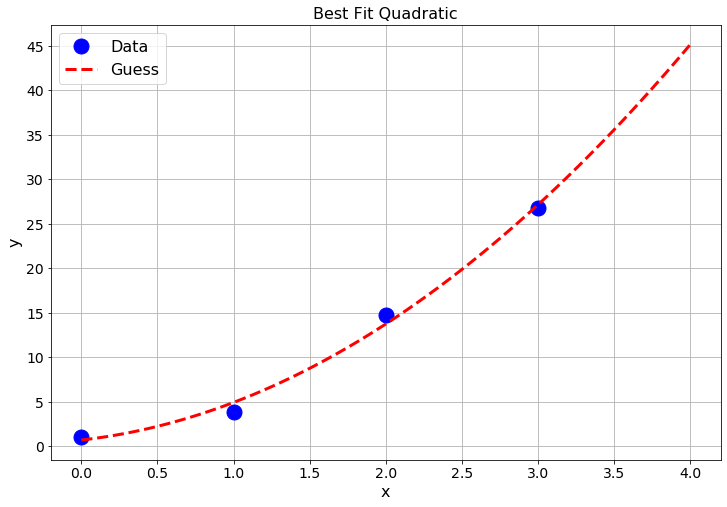
\includegraphics[width=0.75\linewidth]{images/Ch03_BestQuadratic} 

}

\caption{Best fit quadratic function.}\label{fig:unnamed-chunk-246}
\end{figure}

\begin{center}\rule{0.5\linewidth}{0.5pt}\end{center}

\begin{exercise}
\protect\hypertarget{exr:unnamed-chunk-247}{}{\label{exr:unnamed-chunk-247} }With a partner choose a function and then choose 10 points on that function. Add a small bit of error into the \(y\)-values of your points. Give your 10 points to another group. Upon receiving your new points:

\begin{itemize}
\tightlist
\item
  Plot your points.
\item
  Make a guess about the basic form of the function that might best fit the data. Your general form will likely have several parameters (just like the quadratic had the parameters \(a\), \(b\), and \(c\)).\\
\item
  Modify the code from above to find the best collection of parameters minimize the sum of the squares of the residuals between your function and the data.\\
\item
  Plot the data along with your best fit function. If you are not satisfied with how it fit then make another guess on the type of function and repeat the process.
\item
  Finally, go back to the group who gave you your points and check your work.
\end{itemize}
\end{exercise}

\begin{center}\rule{0.5\linewidth}{0.5pt}\end{center}

\begin{exercise}
\protect\hypertarget{exr:unnamed-chunk-248}{}{\label{exr:unnamed-chunk-248} }Your instructor will now give you a collection of dataset. For each dataset give a functional form that might be a good model for the data. Be sure to choose the most general form of your guess (for example, if you choose ``quadratic'' then your functional guess is \(f(x) = ax^2 + bx + c\) or if you choose sinusoidal then your guess should be something like \(f(x) = A\sin(Bx) + C\cos(Dx) + E\).). Once you have a guess of the function type create a plot showing your data along with your guess for a reasonable set of parameters. Then write a function that leverages \texttt{scipy.optimize.minimize()} to find the best set of parameters so that your function best fits the data.
\end{exercise}

\begin{center}\rule{0.5\linewidth}{0.5pt}\end{center}

\hypertarget{exercises-2}{%
\section{Exercises}\label{exercises-2}}

\hypertarget{algorithm-summaries-1}{%
\subsection{Algorithm Summaries}\label{algorithm-summaries-1}}

\begin{exercise}
\protect\hypertarget{exr:unnamed-chunk-249}{}{\label{exr:unnamed-chunk-249} }Starting from Taylor series prove that
\[f'(x) \approx \frac{f(x+h) - f(x)}{h}\] is a first-order approximation
of the first derivative of \(f(x)\). Clearly describe what ``first-order
approximation'' means in this context.
\end{exercise}

\begin{center}\rule{0.5\linewidth}{0.5pt}\end{center}

\begin{exercise}
\protect\hypertarget{exr:unnamed-chunk-250}{}{\label{exr:unnamed-chunk-250} }Starting from Taylor series prove that
\[f'(x) \approx \frac{f(x+h) - f(x-h)}{2h}\] is a second-order
approximation of the first derivative of \(f(x)\). Clearly describe what
``second-order approximation'' means in this context.
\end{exercise}

\begin{center}\rule{0.5\linewidth}{0.5pt}\end{center}

\begin{exercise}
\protect\hypertarget{exr:unnamed-chunk-251}{}{\label{exr:unnamed-chunk-251} }Starting from Taylor series prove that
\[f''(x) \approx \frac{f(x+h) - 2f(x) + f(x-h)}{h^2}\] is a second-order
approximation of the second derivative of \(f(x)\). Clearly describe what
``second-order approximation'' means in this context.
\end{exercise}

\begin{center}\rule{0.5\linewidth}{0.5pt}\end{center}

\begin{exercise}
\protect\hypertarget{exr:unnamed-chunk-252}{}{\label{exr:unnamed-chunk-252} }Explain how to approximate the value of a definite integral with Riemann
sums. When will the Riemann sum approximation be exact? The Riemann sum
approximation is first order. Expain what ``first order'' means for
calculating a definite integral.
\end{exercise}

\begin{center}\rule{0.5\linewidth}{0.5pt}\end{center}

\begin{exercise}
\protect\hypertarget{exr:unnamed-chunk-253}{}{\label{exr:unnamed-chunk-253} }Explain how to approximate the value of a definite integral with the
Trapezoid rule. When will the Trapezoid rule approximation be exact? The
Trapezoidal rule approximation is second order. Expain what ``second
order'' means for calculating a definite integral.
\end{exercise}

\begin{center}\rule{0.5\linewidth}{0.5pt}\end{center}

\begin{exercise}
\protect\hypertarget{exr:unnamed-chunk-254}{}{\label{exr:unnamed-chunk-254} }Explain how to approximate the value of a definite integral with
Simpson's rule. Give the full mathematical details for where Simpson's
rule comes from. When will the Simpson's rule approximation be exact?
The Simpson's rule approximation is fourth order. Expain what ``fourth
order'' means for calculating a definite integral.
\end{exercise}

\begin{center}\rule{0.5\linewidth}{0.5pt}\end{center}

\begin{exercise}
\protect\hypertarget{exr:unnamed-chunk-255}{}{\label{exr:unnamed-chunk-255} }Explain in clear language how the derivative free optimization method
works on a single-variable function.
\end{exercise}

\begin{center}\rule{0.5\linewidth}{0.5pt}\end{center}

\begin{exercise}
\protect\hypertarget{exr:unnamed-chunk-256}{}{\label{exr:unnamed-chunk-256} }Explain in clear language how the gradient descent/ascent optimization
method works on a single-variable function.
\end{exercise}

\begin{center}\rule{0.5\linewidth}{0.5pt}\end{center}

\begin{exercise}
\protect\hypertarget{exr:unnamed-chunk-257}{}{\label{exr:unnamed-chunk-257} }Explain in clear language how the Monte Carlo search optimization method
works on a single-variable function.
\end{exercise}

\begin{center}\rule{0.5\linewidth}{0.5pt}\end{center}

\begin{exercise}
\protect\hypertarget{exr:unnamed-chunk-258}{}{\label{exr:unnamed-chunk-258} }Explain in clear language how you find the optimal set of parameters
given a set of data and a proposed general function type.
\end{exercise}

\begin{center}\rule{0.5\linewidth}{0.5pt}\end{center}

\hypertarget{applying-what-youve-learned-2}{%
\subsection{Applying What You've Learned}\label{applying-what-youve-learned-2}}

\begin{exercise}
\protect\hypertarget{exr:unnamed-chunk-259}{}{\label{exr:unnamed-chunk-259} }For each of the following numerical differentiation formulas (1) prove
that the formula is true and (2) find the order of the method. To prove
that each of the formulas is true you will need to write the Taylor
series for all of the terms in the numerator on the right and then
simplify to solve for the necessary derivative. The highest power of the
remainder should reveal the order of the method.

\begin{enumerate}
\def\labelenumi{\alph{enumi}.}
\item
  \(f'(x) \approx \frac{\frac{1}{12} f(x-2h) - \frac{2}{3} f(x-h) +  \frac{2}{3} f(x+h) - \frac{1}{12} f(x+2h)}{h}\)
\item
  \(f'(x) \approx \frac{-\frac{3}{2} f(x) + 2 f(x+h) -  \frac{1}{2} f(x+2h)}{h}\)
\item
  \(f''(x) \approx \frac{-\frac{1}{12} f(x-2h) + \frac{4}{3} f(x-h) -  \frac{5}{2} f(x) + \frac{4}{3} f(x+h) - \frac{1}{12} f(x+2h)}{h^2}\)
\item
  \(f'''(x) \approx \frac{-\frac{1}{2} f(x-2h) + f(x-h) - f(x+h) +  \frac{1}{2} f(x+2h)}{h^3}\)
\end{enumerate}
\end{exercise}

\begin{center}\rule{0.5\linewidth}{0.5pt}\end{center}

\begin{exercise}
\protect\hypertarget{exr:unnamed-chunk-260}{}{\label{exr:unnamed-chunk-260} }Write a function that accepts a list of
\((x,y)\) ordered pairs from a spreadsheet and returns a list of
\((x,y)\) ordered pairs for a first order approximation of the first
derivative of the underlying function. Create a test spreadsheet file and a
test script that have graphical output showing that your function is
finding the correct derivative.
\end{exercise}

\begin{center}\rule{0.5\linewidth}{0.5pt}\end{center}

\begin{exercise}
\protect\hypertarget{exr:unnamed-chunk-261}{}{\label{exr:unnamed-chunk-261} }Write a function that accepts a list of \((x,y)\) ordered pairs from an
Excel spreadsheet and returns a list of \((x,y)\) ordered pairs for a
second order approximation of the second derivative of the underlying
function. Create a test Excel file and a test script that have graphical
output showing that your function is finding the correct derivative.
\end{exercise}

\begin{center}\rule{0.5\linewidth}{0.5pt}\end{center}

\begin{exercise}
\protect\hypertarget{exr:unnamed-chunk-262}{}{\label{exr:unnamed-chunk-262} }Write a function that implements the
trapezoidal rule on a list of \((x,y)\) order pairs representing the
integrand function. The list of ordered pairs should be read from an
Excel file. Create a test Excel file and a test script showing that your
function is finding the correct integral.
\end{exercise}

\begin{center}\rule{0.5\linewidth}{0.5pt}\end{center}

\begin{exercise}
\protect\hypertarget{exr:unnamed-chunk-263}{}{\label{exr:unnamed-chunk-263} }Use numerical integration to answer the question in each of the
following scenarios

\begin{enumerate}
\def\labelenumi{\alph{enumi}.}
\tightlist
\item
  We measure the rate at which water is flowing out of a reservoir (in
  gallons per second) several times over the course of one hour.
  Estimate the total amount of water which left the reservoir during
  that hour.
\end{enumerate}

\begin{longtable}[]{@{}llllllll@{}}
\toprule
time (min) & 0 & 7 & 19 & 25 & 38 & 47 & 55\tabularnewline
\midrule
\endhead
flow rate (gal/sec) & 316 & 309 & 296 & 298 & 305 & 314 & 322\tabularnewline
\bottomrule
\end{longtable}

\begin{enumerate}
\def\labelenumi{\alph{enumi}.}
\setcounter{enumi}{1}
\tightlist
\item
  The department of transportation finds that the rate at which cars
  cross a bridge can be approximated by the function
  \[f(t) = \frac{22.8 }{3.5 + 7(t-1.25)^4} ,\] where \(t=0\) at 4pm, and
  is measured in hours, and \(f(t)\) is measured in cars per minute.
  Estimate the total number of cars that cross the bridge between 4
  and 6pm. Make sure that your estimate has an error less than 5\% and
  provide sufficient mathematical evidence of your error estimate.
\end{enumerate}
\end{exercise}

\begin{center}\rule{0.5\linewidth}{0.5pt}\end{center}

\begin{exercise}
\protect\hypertarget{exr:unnamed-chunk-264}{}{\label{exr:unnamed-chunk-264} }Consider the integrals
\[\int_{-2}^2 e^{-x^2/2} dx \quad \text{and} \quad \int_0^1 \cos(x^2) dx.\]
Neither of these integrals have closed-form solutions so a numerical
method is necessary. Create a loglog plot that shows the errors for the
integrals with different values of \(h\) (log of \(h\) on the \(x\)-axis and
log of the absolute error on the \(y\)-axis). Write a complete
interpretation of the loglog plot. To get the \emph{exact} answer for these
plots use the =0 MATLAB command. Python's \texttt{scipy.integrate.quad}
command. (What we're really doing here is comparing our algorithms to 's
built in algorithm).
\end{exercise}

\begin{center}\rule{0.5\linewidth}{0.5pt}\end{center}

\begin{exercise}
\protect\hypertarget{exr:unnamed-chunk-265}{}{\label{exr:unnamed-chunk-265} }Go to \href{https://www.data.gov/}{data.gov} or the \href{http://apps.who.int/gho/data/?theme=home}{World Health
Organization Data Repository}
and find data sets for the following tasks.

\begin{enumerate}
\def\labelenumi{\alph{enumi}.}
\item
  Find a data set where the variables naturally lead to a meaningful
  derivative. Use appropriate code to evaluate and plot the
  derivative. If your data appears to be subject to significant noise
  then you may want to smooth the data first before doing the derivative. Write a few sentences explaning what the
  derivative means in the context of the data.
\item
  Find a data set where the variables naturally lead to a meaningfun
  definite integral. Use appropriate code to evaluate the definite integral.
  If your data appears to be subject to significant noise then you might want to smooth the data first before doing the
  integral. Write a few sentences explaning what the integral means in
  the context of the data.
\end{enumerate}

In both of these tasks be very cautious of the units on the data sets
and the units of your answer.
\end{exercise}

\begin{center}\rule{0.5\linewidth}{0.5pt}\end{center}

\begin{exercise}
\protect\hypertarget{exr:unnamed-chunk-266}{}{\label{exr:unnamed-chunk-266} }Integrate each of the functions over the interval \([-1,2]\) and verify
mathematically that your numerical integral is correct to 10 decimal
places. Then provide a plot of the function along with its numerical
first derivative.

\begin{enumerate}
\def\labelenumi{\alph{enumi}.}
\item
  \(f(x) = \frac{x}{1+x^4}\)
\item
  \(g(x) = (x-1)^3 (x-2)^2\)
\item
  \(h(x) = \sin\left(x^2\right)\)
\end{enumerate}
\end{exercise}

\begin{center}\rule{0.5\linewidth}{0.5pt}\end{center}

\begin{exercise}
\protect\hypertarget{exr:unnamed-chunk-267}{}{\label{exr:unnamed-chunk-267} }A bicyclist completes a race course in 90 seconds. The speed of the
biker at each 10-second interval is determined using a radar gun and is
given in the table in feet per second. How long is the race course?

\begin{longtable}[]{@{}lllllllllll@{}}
\toprule
Time (sec) & 0 & 10 & 20 & 30 & 40 & 50 & 60 & 70 & 80 & 90\tabularnewline
\midrule
\endhead
Speed (ft/sec) & 34 & 32 & 29 & 33 & 37 & 40 & 41 & 36 & 38 & 39\tabularnewline
\bottomrule
\end{longtable}
\end{exercise}

\begin{center}\rule{0.5\linewidth}{0.5pt}\end{center}

\begin{exercise}
\protect\hypertarget{exr:unnamed-chunk-268}{}{\label{exr:unnamed-chunk-268} }For each of the following functions write code to find the local maximum
or minimum that is closest to \(x=0\). You may want to start with a plot
of the function just to get a feel for where the local extreme value(s)
might be.

\begin{enumerate}
\def\labelenumi{\alph{enumi}.}
\item
  \(\displaystyle f(x) = \frac{x}{1+x^4} + \sin(x)\)
\item
  \(\displaystyle g(x) =  \left(x-1\right)^3\cdot\left(x-2\right)^2+e^{-0.5\cdot x}\)
\end{enumerate}
\end{exercise}

\begin{center}\rule{0.5\linewidth}{0.5pt}\end{center}

\begin{exercise}
\protect\hypertarget{exr:unnamed-chunk-269}{}{\label{exr:unnamed-chunk-269} }Go back to your old Calculus textbook or homework and find your favorite
optimization problem. State the problem, create the mathematical model,
and use any of the numerical optimization techniques in this chapter to
get an approximate solution to the problem.
\end{exercise}

\begin{center}\rule{0.5\linewidth}{0.5pt}\end{center}

\begin{exercise}
\protect\hypertarget{exr:unnamed-chunk-270}{}{\label{exr:unnamed-chunk-270} }Your instructor will give you access to several sets of noisy data from
measurements of elementary single variable functions.

\begin{enumerate}
\def\labelenumi{\alph{enumi}.}
\item
  Make a hypothesis about which function would best model the data. Be
  sure to choose the most general (parameterized) form of your
  function.
\item
  Use appropriate tools to find the parameters for the function that
  best fits the data. Report you sum of square residuals for each
  function.
\end{enumerate}

Your instructor will provide you with the raw data. The functions that you propose must be continuous functions.
\end{exercise}

\begin{center}\rule{0.5\linewidth}{0.5pt}\end{center}

\hypertarget{projects-1}{%
\section{Projects}\label{projects-1}}

In this section we propose several ideas for projects related to
numerical Calculus. These projects are meant to be open ended, to
encourage creative mathematics, to push your coding skills, and to
require you to write and communicate your mathematics. Take the time to
read Appendix \ref{ch:writing} before you write your final solution.

\hypertarget{galaxy-integration}{%
\subsection{Galaxy Integration}\label{galaxy-integration}}

To analyze the light from stars and galaxies, scientists use a spectral
grating (fancy prism) to split it up into the different frequencies
(colors). We can then measure the intensity (brightness) of the light
(in units of Watts per square meter) at each frequency (measured in
Hertz), to get intensity per frequency (Watts per square meter per
Hertz, W/(m\(^2\) Hz)). Light from the dense opaque surface of a star
produces a smooth rainbow, which produces a continuous curve when we
plot intensity versus frequency. However stars are also surrounded by
thin gas which either emits or absorbs light at only a specific set of
frequencies, called spectral lines. Every chemical element produces a
specific set of lines (or peaks) at fixed frequencies, so by identifying
the lines, we can tell what types of atoms and molecules a star is made
of. If the gas is cool, then it will absorb light at these wavelengths,
and if the gas is hot then it will emit light at these wavelengths. For
galaxies, on the other hand, we expect mostly emission spectra: light
emitted from the galaxy.

For this project we will be analyzing the galaxy ``ngc 1275''. The black
hole at the center of this galaxy is often referred to as the ``Galactic
Spaghetti Monster'' since the magnetic field ``sustains a mammoth network
of spaghetti-like gas filaments around it''. In the Excel file
associated with this project you will see the spectral data measuring
the light intensity from ncg 1275 at several different wavelengths
(measured in Angstroms ). You will notice in this data set that there
are several emission lines at various wavelengths. Of particular
interest are the peaks near \(3800\) Angstroms, \(5100\) Angstroms, \(6400\)
Angstroms, and the two peaks around \(6700\) Angstroms. The data set
contains 1,727 data points at different wavelengths. Your first job will
be to transform the wavelength data to frequency via the formula
\[\lambda = \frac{c}{f}\] where \(\lambda\) is the wavelength, \(c\) is the
speed of light, and \(f\) is the frequency (measured in Hertz). Be sure to
double check the units. Given the inverse relationship between frequency
and wavelength you should see the emission lines flip to the other side
of the plot (right-to-left or left-to-right).

The strength of each emission line (in W/m\(^2\)) is defined as the
relative intensity of each peak across the associated frequencies. Note
that you are not interested in the intensity of the continuous spectrum
-- just the peaks. That is to say that you are only interested in the
area above the background curve and the background noise.

Your primary task is to develop a process for analyzing data sets like
this so as to determine the strength of each emission lines. You must
demonstrate your process on this particular data set, but your process
must be generalizable to any similar data set. Your process must clearly
determine the strength of peaks in data sets like this and you must
apply your procedure to determine the strength of each of these four
lines with an associated margin of error. Keep in mind that you will
first want to first develop a method for removing the background noise.
Finally, the double peak near \(6700\) Angstroms needs to be handled with
care: the strength of each emission line is only the integral over one
peak, not two, so you'll need to determine a way to separate these
peaks.

Finally, it would be cool, but is not necessary, to report on which
chemicals correspond to the emission lines in the data. Remember that
the galaxy is far away and hence there is a non-trivial red-shift to
consider. This will take some research but if done properly will likely
give a lot more merit to your paper.

\hypertarget{higher-order-integration}{%
\subsection{Higher Order Integration}\label{higher-order-integration}}

Riemann sums can be used to approximate integrals and they do so by
using piece wise constant functions to approximate the function. The
trapezoidal rule uses piece wise linear functions to approximate the
function and then the area of a trapezoid to approximate the area. We
saw earlier that Simpson's rule uses piece wise parabolas to approximate
the function. The process which we used to build Simpson's rule can be
extended to any higher-order polynomial. Your job in this project is to
build integration algorithms that use piece wise cubic functions, quartic
functions, etc. For each you need to show all of the mathematics
necessary to derive the algorithm, provide several test cases to show
that the algorithm works, and produce a numerical experiment that shows
the order of accuracy of the algorithm.

\hypertarget{dam-integration}{%
\subsection{Dam Integration}\label{dam-integration}}

Go to the USGS water data repository:\\
\url{https://maps.waterdata.usgs.gov/mapper/index.html}.\\
Here you'll find a map with information about water resources around the
country.

\begin{itemize}
\item
  Zoom in to a dam of your choice (make sure that it is a dam).
\item
  Click on the map tag then click ``Access Data''
\item
  From the drop down menu at the top select either ``Daily Data'' or
  ``Current / Historical Data''. If these options don't appear then
  choose a different dam.
\item
  Change the dates so you have the past year's worth of information.
\item
  Select ``Tab-separated'' under ``Output format'' and press Go. Be sure
  that the data you got has a flow rate (ft\(^3\)/sec).
\item
  At this point you should have access to the entire data set. Copy it
  into a \texttt{csv} file and save it to your computer.
\end{itemize}

For the data that you just downloaded you have three tasks: (1) plot the
data in a reasonable way giving appropriate units, (2) find the total
amount of water that has been discharged from the dam during the past
calendar year, and (3) report any margin of error in your calculation
based on the numerical method that you used in part (2).

\hypertarget{edge-detection-in-images}{%
\subsection{Edge Detection in Images}\label{edge-detection-in-images}}

Edge detection is the process of finding the boundaries or edges of objects in an image. There are many approaches to performing edge detection, but one method that is quite robust is to use the gradient vector in the following way:

\begin{itemize}
\tightlist
\item
  First convert the image to grayscale.
\item
  Then think of the grayscale image as a plot of a multivariable function \(G(x,y)\) where the ordered pair \((x,y)\) is the pixel location and the output \(G(x,y)\) is the value of the grayscale at that point.
\item
  At each pixel calculate the gradient of the function \(G(x,y)\) numerically.
\item
  If the magnitude of the gradient is larger than some threshold then the function \(G(x,y)\) is steep at that location and it is possible that there is an edge (a transition from one part of the image to a different part) at that point. Hence, if \(\|\nabla G(x,y)\| > \delta\) for some threshold \(\delta\) then we can mark the point \((x,y)\) as an edge point.
\end{itemize}

\textbf{Your Tasks:}

\begin{enumerate}
\def\labelenumi{\arabic{enumi}.}
\tightlist
\item
  Choose several images on which to do edge detection. You should take your own images, but if you choose not to be sure that you cite the source(s) of your images.
\item
  Write Python code that performs edge detection as described above on the image. In the end you should produce side-by-side plots of the original picture and the image showing only the edges. To calculate the gradient use a centered difference scheme for the first derivatives
  \[ f'(x) \approx \frac{f(x+h)-f(x-h)}{2h}. \]
  In an image we can take \(h=1\) (why?), and since the gradient is two dimensional we get
  \[ \nabla G(x,y) \approx \left< \frac{G(x+1,y)-G(x-1,y)}{2} \, , \, \frac{G(x,y+1)-G(x,y-1)}{2}  \right>. \]
\item
  There are many ways to approximate numerical first derivatives. The simplest approach is what you did in part (2) -- using a centered difference scheme. However, pixels are necessarily tightly packed in an image and the immediate neighbors of a point may not have enough contrast to truly detect edges. Your job is to build several other approaches to calculating the gradient vector, implement them to perform edge detection, and show the resulting images. For each method you need to give the full mathematical details for how you calculated the gradient as well as give a list of pros and cons for using the new numerical gradient for edge detection based on what you see in your images. As an example, you could use a centered difference scheme that looks two pixels away instead of at the immediate neighboring pixels
  \[ f'(x) \approx \frac{??? f(x-2) + ??? f(x+2)}{???}. \]
  Of course you would need to determine the coefficients in this approximation scheme.\\
  Another idea could use a centered difference scheme that uses pixels that are immediate neighbors AND pixels that are two units away
  \[ f'(x) \approx \frac{??? f(x-2) + ??? f(x-1) + ??? f(x+1) + ??? f(x+2)}{???}. \]\\
  In any case, you will need to use Taylor Series to derive coefficients in the formulas for the derivatives as well as the order of the error. There are many ways to approximate the first derivatives so be creative. You are not restricted to using just the first derivative either. There could be some argument for using the second derivatives of the grayscale image function \(G(x,y)\) and using some function of the concavity as a means of edge detection. Explore and have fun!
\end{enumerate}

The following code will allow you to read an image into Python as an \texttt{np.array()}.

\begin{Shaded}
\begin{Highlighting}[]
\ImportTok{import}\NormalTok{ numpy }\ImportTok{as}\NormalTok{ np}
\ImportTok{import}\NormalTok{ matplotlib.pyplot }\ImportTok{as}\NormalTok{ plt}
\ImportTok{from}\NormalTok{ matplotlib }\ImportTok{import}\NormalTok{ image}
\NormalTok{I }\OperatorTok{=}\NormalTok{ np.array(image.imread(}\StringTok{\textquotesingle{}ImageName.jpg\textquotesingle{}}\NormalTok{))}
\NormalTok{plt.imshow(I)}
\NormalTok{plt.axis(}\StringTok{"off"}\NormalTok{)}
\NormalTok{plt.show()}
\end{Highlighting}
\end{Shaded}

You should notice that the image, \texttt{I}, is a three dimensional array. The three layers are the red, green, and blue channels of the image. To flatten the image to grayscale you can apply the rule
\[ \text{grayscale value} = 0.3 \text{Red} + 0.59 \text{Green} + 0.11 \text{Blue}. \]
The output should be a 2 dimensional \texttt{numpy} array which you can show with the following Python code.

\begin{Shaded}
\begin{Highlighting}[]
\NormalTok{plt.imshow(G, cmap}\OperatorTok{=}\StringTok{\textquotesingle{}gray\textquotesingle{}}\NormalTok{) }\CommentTok{\# "cmap" stands for "color map"}
\NormalTok{plt.axis(}\StringTok{"off"}\NormalTok{)}
\NormalTok{plt.show()}
\end{Highlighting}
\end{Shaded}

Figure \ref{fig:edgedetection} shows the result of different threshold values applied to the simplest numerical gradient computations. The image was taken by the author.

\begin{figure}

{\centering 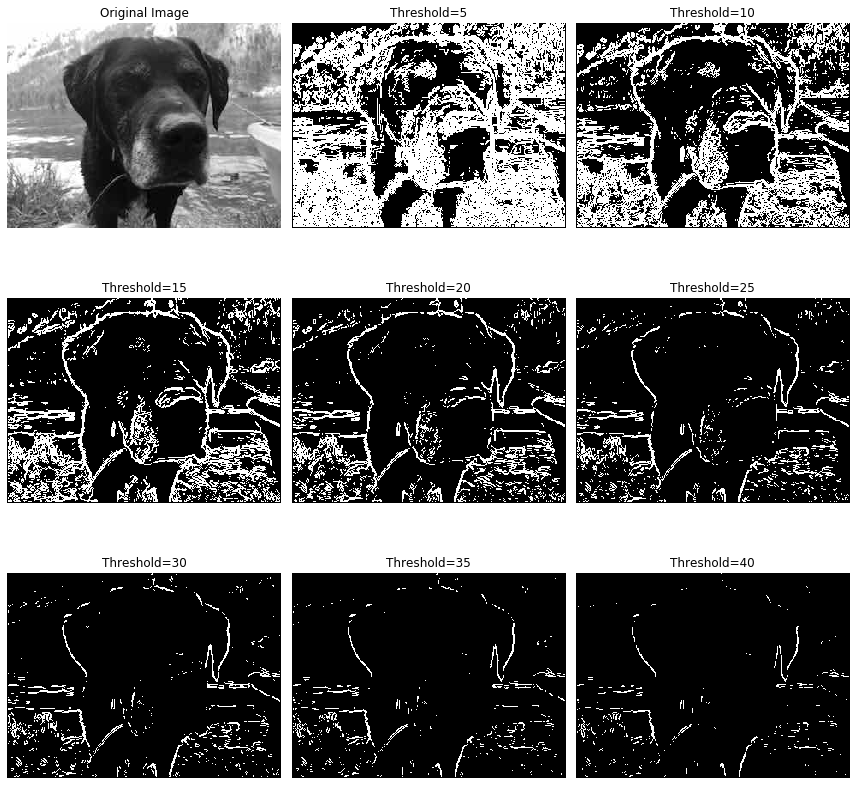
\includegraphics[width=0.85\linewidth]{images/Ch03_EdgeDetection} 

}

\caption{Edge detection using different thresholds for the value of the gradient on the grayscale image}\label{fig:edgedetection}
\end{figure}

\hypertarget{ch:linearalgebra}{%
\chapter{Linear Algebra}\label{ch:linearalgebra}}

\hypertarget{intro-to-numerical-linear-algebra}{%
\section{Intro to Numerical Linear Algebra}\label{intro-to-numerical-linear-algebra}}

\begin{quote}
\emph{You cannot learn too much linear algebra.}\\
-- Every mathematician
\end{quote}

The preceding comment says it all -- linear algebra is the most important of all of the mathematical tools that you can learn as a practitioner of the mathematical sciences.. The theorems, proofs, conjectures, and big ideas in almost every other mathematical field find their roots in linear algebra. Our goal in this chapter is to explore numerical algorithms for the primary questions of
linear algebra:

\begin{itemize}
\tightlist
\item
  solving systems of equations,
\item
  approximating solutions to over-determined systems of equations, and
\item
  finding the dominant eigenvalue-eigenvector pair for a matrix.
\end{itemize}

Take careful note, that in our current digital age numerical linear algebra and its fast algorithms are behind the scenes for wide varieties of computing applications. Applications of numerical linear algebra include:

\begin{itemize}
\tightlist
\item
  determining the most important web page in a Google search,
\item
  determine the forces on a car during a crash,
\item
  modeling realistic 3D environments in video games,
\item
  digital image processing,
\item
  building neural networks and AI algorithms,
\item
  and many many more.
\end{itemize}

What's more, researchers have found provably optimal ways to perform most of the typical tasks of linear algebra so most scientific software works very well and very quickly with linear algebra. For example, we have already seen in Chapter \ref{ch:calculus} that programming numerical differentiation and numerical integration schemes can be done in Python with the use of vectors instead of loops. We want to use vectors specifically so that we can use the fast implementations of numerical linear algebra in the background in Python.

Lastly, a comment on notation. Throughout this chapter we will use the following notation conventions.

\begin{itemize}
\tightlist
\item
  A bold mathematical symbol such as \(\boldsymbol{x}\) or \(\boldsymbol{u}\) will represent a vector.\\
\item
  If \(\boldsymbol{u}\) is a vector then \(u_j\) will be the \(j^{th}\) entry of the vector.
\item
  Vectors will typically be written vertically with parenthesis as delimiters such as
  \[ \boldsymbol{u} = \begin{pmatrix} 1\\2\\3 \end{pmatrix}. \]
\item
  Two bold symbols separated by a centered dot such as \(\boldsymbol{u} \cdot \boldsymbol{v}\) will represent the dot product of two vectors.
\item
  A capital mathematical symbol such as \(A\) or \(X\) will represent a matrix
\item
  If \(A\) is a matrix then \(A_{ij}\) will be the element in the \(i^{th}\) row and \(j^{th}\) column of the matrix.
\item
  A matrix will typically be written with parenthesis as delimiters such as
  \[ A = \begin{pmatrix} 1 & 2 & 3 \\ 4 & 5 & \pi \end{pmatrix}. \]
\item
  The juxtaposition of a capital symbol and a bold symbol such as \(A\boldsymbol{x}\) will represent matrix-vector multiplication.
\item
  A lower case or Greek mathematical symbol such as \(x\), \(c\), or \(\lambda\) will represent a scalar.\\
\item
  The scalar field of real numbers is given as \(\mathbb{R}\) and the scalar field of complex numbers is given as \(\mathbb{C}\).\\
\item
  The symbol \(\mathbb{R}^n\) represents the collection of \(n\)-dimensional vectors where the elements are drawn from the real numbers.\\
\item
  The symbol \(\mathbb{C}^n\) represents the collection of \(n\)-dimensional vectors where the elements are drawn from the complex numbers.
\end{itemize}

It is an important part of learning to read and write linear algebra to give special attention to the symbolic language so you can communicate your work easily and efficiently.

\hypertarget{vectors-and-matrices-in-python}{%
\section{Vectors and Matrices in Python}\label{vectors-and-matrices-in-python}}

We first need to understand how Python's \texttt{numpy} library builds and stores vectors and matrices. The following exercises will give you some experience building and working with these data structures and will point out some common pitfalls that mathematicians fall into when using Python for linear algebra.

\begin{center}\rule{0.5\linewidth}{0.5pt}\end{center}

\begin{example}[`numpy` Arrays]
\protect\hypertarget{exm:unnamed-chunk-273}{}{\label{exm:unnamed-chunk-273} \iffalse (\texttt{numpy} Arrays) \fi{} }In Python you can build a list using square brackets such as \texttt{{[}1,2,3{]}}. This is called a ``Python list'' and is NOT a vector in the way that we think about it mathematically. It is simply an ordered collection of objects. To build mathematical vectors in Python we need to use \texttt{numpy} arrays with \texttt{np.array()}. For example, the vector
\[ \boldsymbol{u} = \begin{pmatrix} 1\\2\\3\end{pmatrix} \]
would be built with the following code.
\end{example}

\begin{Shaded}
\begin{Highlighting}[]
\ImportTok{import}\NormalTok{ numpy }\ImportTok{as}\NormalTok{ np}
\NormalTok{u }\OperatorTok{=}\NormalTok{ np.array([}\DecValTok{1}\NormalTok{,}\DecValTok{2}\NormalTok{,}\DecValTok{3}\NormalTok{])}
\BuiltInTok{print}\NormalTok{(u)}
\end{Highlighting}
\end{Shaded}

\begin{verbatim}
## [1 2 3]
\end{verbatim}

Notice that Python defines the vector \texttt{u} as a matrix without a second dimension. You can see that in the following code.

\begin{Shaded}
\begin{Highlighting}[]
\ImportTok{import}\NormalTok{ numpy }\ImportTok{as}\NormalTok{ np}
\NormalTok{u }\OperatorTok{=}\NormalTok{ np.array([}\DecValTok{1}\NormalTok{,}\DecValTok{2}\NormalTok{,}\DecValTok{3}\NormalTok{])}
\BuiltInTok{print}\NormalTok{(}\StringTok{"The length of the u vector is }\CharTok{\textbackslash{}n}\StringTok{"}\NormalTok{,}\BuiltInTok{len}\NormalTok{(u))}
\end{Highlighting}
\end{Shaded}

\begin{verbatim}
## The length of the u vector is 
##  3
\end{verbatim}

\begin{Shaded}
\begin{Highlighting}[]
\BuiltInTok{print}\NormalTok{(}\StringTok{"The shape of the u vector is }\CharTok{\textbackslash{}n}\StringTok{"}\NormalTok{,u.shape)}
\end{Highlighting}
\end{Shaded}

\begin{verbatim}
## The shape of the u vector is 
##  (3,)
\end{verbatim}

\begin{center}\rule{0.5\linewidth}{0.5pt}\end{center}

\begin{example}[`numpy` Matrices]
\protect\hypertarget{exm:unnamed-chunk-276}{}{\label{exm:unnamed-chunk-276} \iffalse (\texttt{numpy} Matrices) \fi{} }In \texttt{numpy}, a matrix is a list of lists. For example, the matrix
\[ A = \begin{pmatrix} 1 & 2 & 3 \\ 4 & 5 & 6 \\ 7 & 8 & 9 \end{pmatrix} \]
is defined using \texttt{np.matrix()} where each row is an individual list, and the matrix is a collection of these lists.
\end{example}

\begin{Shaded}
\begin{Highlighting}[]
\ImportTok{import}\NormalTok{ numpy }\ImportTok{as}\NormalTok{ np}
\NormalTok{A }\OperatorTok{=}\NormalTok{ np.matrix([[}\DecValTok{1}\NormalTok{,}\DecValTok{2}\NormalTok{,}\DecValTok{3}\NormalTok{],[}\DecValTok{4}\NormalTok{,}\DecValTok{5}\NormalTok{,}\DecValTok{6}\NormalTok{],[}\DecValTok{7}\NormalTok{,}\DecValTok{8}\NormalTok{,}\DecValTok{9}\NormalTok{]])}
\BuiltInTok{print}\NormalTok{(A)}
\end{Highlighting}
\end{Shaded}

\begin{verbatim}
## [[1 2 3]
##  [4 5 6]
##  [7 8 9]]
\end{verbatim}

Moreover, we can extract the shape, the number of rows, and the number of columns of \(A\) using the \texttt{A.shape} command. To be a bit more clear on this one we'll use the matrix
\[ A = \begin{pmatrix} 1 & 2 & 3 \\ 4 & 5 & 6 \end{pmatrix} \]

\begin{Shaded}
\begin{Highlighting}[]
\ImportTok{import}\NormalTok{ numpy }\ImportTok{as}\NormalTok{ np}
\NormalTok{A }\OperatorTok{=}\NormalTok{ np.matrix([[}\DecValTok{1}\NormalTok{,}\DecValTok{2}\NormalTok{,}\DecValTok{3}\NormalTok{],[}\DecValTok{4}\NormalTok{,}\DecValTok{5}\NormalTok{,}\DecValTok{6}\NormalTok{]])}
\BuiltInTok{print}\NormalTok{(}\StringTok{"The shape of the A matrix is }\CharTok{\textbackslash{}n}\StringTok{"}\NormalTok{,A.shape)}
\end{Highlighting}
\end{Shaded}

\begin{verbatim}
## The shape of the A matrix is 
##  (2, 3)
\end{verbatim}

\begin{Shaded}
\begin{Highlighting}[]
\BuiltInTok{print}\NormalTok{(}\StringTok{"Number of rows in A is }\CharTok{\textbackslash{}n}\StringTok{"}\NormalTok{,A.shape[}\DecValTok{0}\NormalTok{])}
\end{Highlighting}
\end{Shaded}

\begin{verbatim}
## Number of rows in A is 
##  2
\end{verbatim}

\begin{Shaded}
\begin{Highlighting}[]
\BuiltInTok{print}\NormalTok{(}\StringTok{"Number of columns in A is }\CharTok{\textbackslash{}n}\StringTok{"}\NormalTok{,A.shape[}\DecValTok{1}\NormalTok{])}
\end{Highlighting}
\end{Shaded}

\begin{verbatim}
## Number of columns in A is 
##  3
\end{verbatim}

\begin{center}\rule{0.5\linewidth}{0.5pt}\end{center}

\begin{example}[Row and Column Vectors in Python]
\protect\hypertarget{exm:unnamed-chunk-279}{}{\label{exm:unnamed-chunk-279} \iffalse (Row and Column Vectors in Python) \fi{} }You can more specifically build row or column vectors in Python using the \texttt{np.matrix()} command and then only specifying one row or column. For example, if you want the vectors
\[ \boldsymbol{u} = \begin{pmatrix} 1\\2\\3\end{pmatrix} \quad \text{and} \quad \boldsymbol{v} = \begin{pmatrix} 4 & 5 & 6 \end{pmatrix} \]
then we would use the following Python code.
\end{example}

\begin{Shaded}
\begin{Highlighting}[]
\ImportTok{import}\NormalTok{ numpy }\ImportTok{as}\NormalTok{ np}
\NormalTok{u }\OperatorTok{=}\NormalTok{ np.matrix([[}\DecValTok{1}\NormalTok{],[}\DecValTok{2}\NormalTok{],[}\DecValTok{3}\NormalTok{]])}
\BuiltInTok{print}\NormalTok{(}\StringTok{"The column vector u is }\CharTok{\textbackslash{}n}\StringTok{"}\NormalTok{,u)}
\end{Highlighting}
\end{Shaded}

\begin{verbatim}
## The column vector u is 
##  [[1]
##  [2]
##  [3]]
\end{verbatim}

\begin{Shaded}
\begin{Highlighting}[]
\NormalTok{v }\OperatorTok{=}\NormalTok{ np.matrix([[}\DecValTok{1}\NormalTok{,}\DecValTok{2}\NormalTok{,}\DecValTok{3}\NormalTok{]])}
\BuiltInTok{print}\NormalTok{(}\StringTok{"The row vector v is }\CharTok{\textbackslash{}n}\StringTok{"}\NormalTok{,v)}
\end{Highlighting}
\end{Shaded}

\begin{verbatim}
## The row vector v is 
##  [[1 2 3]]
\end{verbatim}

Alternatively, if you want to define a column vector you can define a row vector (since there are far fewer brackets to keep track of) and then transpose the matrix to turn it into a column.

\begin{Shaded}
\begin{Highlighting}[]
\ImportTok{import}\NormalTok{ numpy }\ImportTok{as}\NormalTok{ np}
\NormalTok{u }\OperatorTok{=}\NormalTok{ np.matrix([[}\DecValTok{1}\NormalTok{,}\DecValTok{2}\NormalTok{,}\DecValTok{3}\NormalTok{]])}
\NormalTok{u }\OperatorTok{=}\NormalTok{ u.transpose()}
\BuiltInTok{print}\NormalTok{(}\StringTok{"The column vector u is }\CharTok{\textbackslash{}n}\StringTok{"}\NormalTok{,u)}
\end{Highlighting}
\end{Shaded}

\begin{verbatim}
## The column vector u is 
##  [[1]
##  [2]
##  [3]]
\end{verbatim}

\begin{center}\rule{0.5\linewidth}{0.5pt}\end{center}

\begin{example}[Matrix Indexing]
\protect\hypertarget{exm:unnamed-chunk-282}{}{\label{exm:unnamed-chunk-282} \iffalse (Matrix Indexing) \fi{} }Python indexes all arrays, vectors, lists, and matrices starting from index 0. Let's get used to this fact.

Consider the matrix \(A\) defined in the previous problem. Mathematically we know that the entry in row 1 column 1 is a 1, the entry in row 1 column 2 is a 2, and so on. However, with Python we need to shift the way that we enumerate the rows and columns of a matrix. Hence we would say that the entry in row 0 column 0 is a 1, the entry in row 0 column 1 is a 2, and so on.

Mathematically we can view all Python matrices as follows. If \(A\) is an \(n \times n\) matrix then
\[ A = \begin{pmatrix} A_{0,0} & A_{0,1} & A_{0,2} & \cdots & A_{0,n-1} \\
A_{1,0} & A_{1,1} & A_{1,2} & \cdots & A_{1,n-1} \\ 
\vdots & \vdots & \vdots & \ddots & \vdots \\
A_{n-1,0} & A_{n-1,1} & A_{n-1,2} & \cdots & A_{n-1,n-1} \end{pmatrix} \]

Similarly, we can view all vectors as follows. If \(\boldsymbol{u}\) is an \(n \times 1\) vector then
\[ \boldsymbol{u} = \begin{pmatrix} u_0 \\ u_1 \\ \vdots \\ u_{n-1} \end{pmatrix} \]
\end{example}

The following code should help to illustrate this indexing convention.

\begin{Shaded}
\begin{Highlighting}[]
\ImportTok{import}\NormalTok{ numpy }\ImportTok{as}\NormalTok{ np}
\NormalTok{A }\OperatorTok{=}\NormalTok{ np.matrix([[}\DecValTok{1}\NormalTok{,}\DecValTok{2}\NormalTok{,}\DecValTok{3}\NormalTok{],[}\DecValTok{4}\NormalTok{,}\DecValTok{5}\NormalTok{,}\DecValTok{6}\NormalTok{],[}\DecValTok{7}\NormalTok{,}\DecValTok{8}\NormalTok{,}\DecValTok{9}\NormalTok{]])}
\BuiltInTok{print}\NormalTok{(}\StringTok{"Entry in row 0 column 0 is"}\NormalTok{,A[}\DecValTok{0}\NormalTok{,}\DecValTok{0}\NormalTok{])}
\end{Highlighting}
\end{Shaded}

\begin{verbatim}
## Entry in row 0 column 0 is 1
\end{verbatim}

\begin{Shaded}
\begin{Highlighting}[]
\BuiltInTok{print}\NormalTok{(}\StringTok{"Entry in row 0 column 1 is"}\NormalTok{,A[}\DecValTok{0}\NormalTok{,}\DecValTok{1}\NormalTok{])}
\end{Highlighting}
\end{Shaded}

\begin{verbatim}
## Entry in row 0 column 1 is 2
\end{verbatim}

\begin{Shaded}
\begin{Highlighting}[]
\BuiltInTok{print}\NormalTok{(}\StringTok{"Entry in the bottom right corner"}\NormalTok{,A[}\DecValTok{2}\NormalTok{,}\DecValTok{2}\NormalTok{])}
\end{Highlighting}
\end{Shaded}

\begin{verbatim}
## Entry in the bottom right corner 9
\end{verbatim}

\begin{center}\rule{0.5\linewidth}{0.5pt}\end{center}

\begin{exercise}
\protect\hypertarget{exr:unnamed-chunk-284}{}{\label{exr:unnamed-chunk-284} }Build your own matrix in Python and practice choosing individual entries from the matrix.
\end{exercise}

\begin{center}\rule{0.5\linewidth}{0.5pt}\end{center}

\begin{example}[Matrix Slicing]
\protect\hypertarget{exm:unnamed-chunk-285}{}{\label{exm:unnamed-chunk-285} \iffalse (Matrix Slicing) \fi{} }The last thing that we need to be familiar with is \emph{slicing} a matrix. The term ``slicing'' gernally refers to pulling out individual rows, columns, entries, or blocks from a list, array, or matrix in Python. Examine the code below to see how to slice parts out of a \texttt{numpy} matrix.
\end{example}

\begin{Shaded}
\begin{Highlighting}[]
\ImportTok{import}\NormalTok{ numpy }\ImportTok{as}\NormalTok{ np}
\NormalTok{A }\OperatorTok{=}\NormalTok{ np.matrix([[}\DecValTok{1}\NormalTok{,}\DecValTok{2}\NormalTok{,}\DecValTok{3}\NormalTok{],[}\DecValTok{4}\NormalTok{,}\DecValTok{5}\NormalTok{,}\DecValTok{6}\NormalTok{],[}\DecValTok{7}\NormalTok{,}\DecValTok{8}\NormalTok{,}\DecValTok{9}\NormalTok{]])}
\BuiltInTok{print}\NormalTok{(A)}
\end{Highlighting}
\end{Shaded}

\begin{verbatim}
## [[1 2 3]
##  [4 5 6]
##  [7 8 9]]
\end{verbatim}

\begin{Shaded}
\begin{Highlighting}[]
\BuiltInTok{print}\NormalTok{(}\StringTok{"The first column of A is }\CharTok{\textbackslash{}n}\StringTok{"}\NormalTok{,A[:,}\DecValTok{0}\NormalTok{])}
\end{Highlighting}
\end{Shaded}

\begin{verbatim}
## The first column of A is 
##  [[1]
##  [4]
##  [7]]
\end{verbatim}

\begin{Shaded}
\begin{Highlighting}[]
\BuiltInTok{print}\NormalTok{(}\StringTok{"The second row of A is }\CharTok{\textbackslash{}n}\StringTok{"}\NormalTok{,A[}\DecValTok{1}\NormalTok{,:])}
\end{Highlighting}
\end{Shaded}

\begin{verbatim}
## The second row of A is 
##  [[4 5 6]]
\end{verbatim}

\begin{Shaded}
\begin{Highlighting}[]
\BuiltInTok{print}\NormalTok{(}\StringTok{"The top left 2x2 sub matrix of A is }\CharTok{\textbackslash{}n}\StringTok{"}\NormalTok{,A[}\DecValTok{0}\NormalTok{:}\OperatorTok{{-}}\DecValTok{1}\NormalTok{,}\DecValTok{0}\NormalTok{:}\OperatorTok{{-}}\DecValTok{1}\NormalTok{])}
\end{Highlighting}
\end{Shaded}

\begin{verbatim}
## The top left 2x2 sub matrix of A is 
##  [[1 2]
##  [4 5]]
\end{verbatim}

\begin{Shaded}
\begin{Highlighting}[]
\BuiltInTok{print}\NormalTok{(}\StringTok{"The bottom right 2x2 sub matrix of A is }\CharTok{\textbackslash{}n}\StringTok{"}\NormalTok{,A[}\DecValTok{1}\NormalTok{:,}\DecValTok{1}\NormalTok{:])}
\end{Highlighting}
\end{Shaded}

\begin{verbatim}
## The bottom right 2x2 sub matrix of A is 
##  [[5 6]
##  [8 9]]
\end{verbatim}

\begin{Shaded}
\begin{Highlighting}[]
\NormalTok{u }\OperatorTok{=}\NormalTok{ np.array([}\DecValTok{1}\NormalTok{,}\DecValTok{2}\NormalTok{,}\DecValTok{3}\NormalTok{,}\DecValTok{4}\NormalTok{,}\DecValTok{5}\NormalTok{,}\DecValTok{6}\NormalTok{])}
\BuiltInTok{print}\NormalTok{(}\StringTok{"The first 3 entries of the vector u are }\CharTok{\textbackslash{}n}\StringTok{"}\NormalTok{,u[}\DecValTok{0}\NormalTok{:}\DecValTok{3}\NormalTok{])}
\end{Highlighting}
\end{Shaded}

\begin{verbatim}
## The first 3 entries of the vector u are 
##  [1 2 3]
\end{verbatim}

\begin{Shaded}
\begin{Highlighting}[]
\BuiltInTok{print}\NormalTok{(}\StringTok{"The last entry of the vector u is }\CharTok{\textbackslash{}n}\StringTok{"}\NormalTok{,u[}\OperatorTok{{-}}\DecValTok{1}\NormalTok{])}
\end{Highlighting}
\end{Shaded}

\begin{verbatim}
## The last entry of the vector u is 
##  6
\end{verbatim}

\begin{Shaded}
\begin{Highlighting}[]
\BuiltInTok{print}\NormalTok{(}\StringTok{"The last two entries of the vector u are }\CharTok{\textbackslash{}n}\StringTok{"}\NormalTok{,u[}\OperatorTok{{-}}\DecValTok{2}\NormalTok{:])}
\end{Highlighting}
\end{Shaded}

\begin{verbatim}
## The last two entries of the vector u are 
##  [5 6]
\end{verbatim}

\begin{center}\rule{0.5\linewidth}{0.5pt}\end{center}

\begin{exercise}
\protect\hypertarget{exr:unnamed-chunk-287}{}{\label{exr:unnamed-chunk-287} }Define the matrix \(A\) and the vector \(u\) in Python. Then perform all of the tasks below.
\[ A = \begin{pmatrix} 1 & 3 & 5 & 7 \\ 2 & 4 & 6 & 8 \\ -3 & -2 & -1 & 0 \end{pmatrix} \quad \text{and} \quad \boldsymbol{u} = \begin{pmatrix} 10\\20\\30 \end{pmatrix} \]

\begin{enumerate}
\def\labelenumi{\alph{enumi}.}
\tightlist
\item
  Print the matrix \(A\), the vector \(\boldsymbol{u}\), the shape of \(A\), and the shape of \(\boldsymbol{u}\).
\item
  Print the first column of \(A\).
\item
  Print the first two rows of \(A\).
\item
  Print the first two entries of \(\boldsymbol{u}\).
\item
  Print the last two entries of \(\boldsymbol{u}\).
\item
  Print the bottom left \(2 \times 2\) submatrix of \(A\).
\item
  Print the middle two elements of the middle row of \(A\).
\end{enumerate}
\end{exercise}

\begin{center}\rule{0.5\linewidth}{0.5pt}\end{center}

\hypertarget{matrix-and-vector-operations}{%
\section{Matrix and Vector Operations}\label{matrix-and-vector-operations}}

Now let's start doing some numerical linear algebra. We start our discussion with the basics: the dot product and matrix multiplication. The numerical routines in Python's \texttt{numpy} packages are designed to do these tasks in very efficient ways but it is a good coding exercise to build your own dot product and matrix multiplication routines just to further cement the way that Python deals with these data structures and to remind you of the mathematical algorithms. What you will find in numerical linear algebra is that the indexing and the housekeeping in the codes is the hardest part. So why don't we start ``easy''.

\hypertarget{the-dot-product}{%
\subsection{The Dot Product}\label{the-dot-product}}

\begin{exercise}
\protect\hypertarget{exr:unnamed-chunk-288}{}{\label{exr:unnamed-chunk-288} }This problem is meant to jog your memory about dot products, how to compute them, and what you might use them for. If your linear algebra is a bit rusty then read ahead a bit and then come back to this problem.

Consider two vectors \(\boldsymbol{u}\) and \(\boldsymbol{v}\) defined as
\[ \boldsymbol{u} = \begin{pmatrix} 1 \\ 2 \end{pmatrix} \quad \text{and} \quad \boldsymbol{v} = \begin{pmatrix} 3\\4 \end{pmatrix}. \]

\begin{enumerate}
\def\labelenumi{\alph{enumi}.}
\tightlist
\item
  Draw a picture showing both \(\boldsymbol{u}\) and \(\boldsymbol{v}\).
\item
  What is \(\boldsymbol{u} \cdot \boldsymbol{v}\)?
\item
  What is \(\|\boldsymbol{u}\|\)?
\item
  What is \(\|\boldsymbol{v}\|\)?
\item
  What is the angle between \(\boldsymbol{u}\) and \(\boldsymbol{v}\)?
\item
  Give two reasons why we know that \(\boldsymbol{u}\) is not perpendicular to \(\boldsymbol{v}\).
\item
  What is the scalar projection of \(\boldsymbol{u}\) onto \(\boldsymbol{v}\)? Draw this scalar projections on your picture from part (a).
\item
  What is the scalar projection of \(\boldsymbol{v}\) onto \(\boldsymbol{u}\)? Draw this scalar projections on your picture from part (a).
\end{enumerate}
\end{exercise}

\begin{center}\rule{0.5\linewidth}{0.5pt}\end{center}

Now let's get the formal definitions of the dot product on the table.

\begin{definition}[The Dot Product]
\protect\hypertarget{def:unnamed-chunk-289}{}{\label{def:unnamed-chunk-289} \iffalse (The Dot Product) \fi{} }The \textbf{dot product} of two vectors \(\boldsymbol{u}, \boldsymbol{v} \in \mathbb{R}^n\) is
\[\boldsymbol{u} \cdot \boldsymbol{v} = \sum_{j=1}^n u_j v_j.\]
Without summation notation the dot product of two vectors is ,
\[\boldsymbol{u} \cdot \boldsymbol{v} = u_1 v_1 + u_2 v_2 + \cdots + u_n v_n.\]
\end{definition}

Alternatively, you may also recall that the dot product of two vectors is given geometrically as
\[ \boldsymbol{u} \cdot \boldsymbol{v} = \|\boldsymbol{u} \| \|\boldsymbol{v}\| \cos \theta \]
where \(\|\boldsymbol{u}\|\) and \(\|\boldsymbol{v}\|\) are the magnitudes (or lengths) of \(\boldsymbol{u}\) and \(\boldsymbol{v}\) respectively, and \(\theta\) is the angle between the two vectors. In physical applications the dot product is often used to find the angle between two vectors (e.g.~between two forces). Hence, the last form of the dot product is often rewritten as
\[ \theta = \cos^{-1}\left( \frac{\boldsymbol{u} \cdot \boldsymbol{v}}{ \|\boldsymbol{u} \| \| \boldsymbol{v} \|} \right). \]

\begin{center}\rule{0.5\linewidth}{0.5pt}\end{center}

\begin{definition}[Magnitude of a Vector]
\protect\hypertarget{def:unnamed-chunk-290}{}{\label{def:unnamed-chunk-290} \iffalse (Magnitude of a Vector) \fi{} }The \textbf{magnitude} of a vector \(\boldsymbol{u} \in \mathbb{R}^n\) is defined as
\[ \| \boldsymbol{u} \| = \sqrt{\boldsymbol{u} \cdot \boldsymbol{u}}. \]
You should note that in two dimensions this collapses to the Pythagorean Theorem, and in higher dimensions this is just a natural extension of the Pythagorean Theorm.\footnote{You should also note that \(\|\boldsymbol{u}\| = \sqrt{\boldsymbol{u} \cdot \boldsymbol{u}}\) is not the only definition of distance. More generally, if you let \(\left< \boldsymbol{u}, \boldsymbol{v}\right>\) be an inner product for \(\boldsymbol{u}\) and \(\boldsymbol{v}\) in some vector space \(\mathcal{V}\) then \(\|\boldsymbol{u}\| = \sqrt{\left< \boldsymbol{u}, \boldsymbol{u}\right>}\). In most cases in this text we will be using the dot product as our prefered inner product so we won't have to worry much about this particular natural extension of the definition of the length of a vector.}
\end{definition}

\begin{center}\rule{0.5\linewidth}{0.5pt}\end{center}

\begin{exercise}
\protect\hypertarget{exr:unnamed-chunk-291}{}{\label{exr:unnamed-chunk-291} }Verify that \(\sqrt{\boldsymbol{u} \cdot \boldsymbol{u}}\) indeed gives the Pythagorean Theorem for \(\boldsymbol{u} \in \mathbb{R}^2\).
\end{exercise}

\begin{center}\rule{0.5\linewidth}{0.5pt}\end{center}

\begin{exercise}
\protect\hypertarget{exr:unnamed-chunk-292}{}{\label{exr:unnamed-chunk-292} }Our task now is to write a Python function that accepts two vectors (defined as \texttt{numpy} arrays) and returns the dot product. Write this code without the use any loops.
\end{exercise}

\begin{Shaded}
\begin{Highlighting}[]
\ImportTok{import}\NormalTok{ numpy }\ImportTok{as}\NormalTok{ np}
\KeywordTok{def}\NormalTok{ myDotProduct(u,v):}
    \ControlFlowTok{return} \CommentTok{\# the dot product formula uses a product inside a sum ... write one line of code here.}
\end{Highlighting}
\end{Shaded}

\begin{center}\rule{0.5\linewidth}{0.5pt}\end{center}

\begin{exercise}
\protect\hypertarget{exr:unnamed-chunk-294}{}{\label{exr:unnamed-chunk-294} }Test your \texttt{myDotProduct()} function on several dot products to make sure that it works. Example code to find the dot product between
\[ \boldsymbol{u} = \begin{pmatrix} 1 \\ 2\\ 3\end{pmatrix} \quad \text{and} \quad \boldsymbol{v} = \begin{pmatrix} 4\\5\\6\end{pmatrix} \]
is given below. Test your code on other vectors. Then implement an error catch into your code to catch the case where the two input vectors are not the same size. You will want to use the \texttt{len()} command to find the length of the vectors.
\end{exercise}

\begin{Shaded}
\begin{Highlighting}[]
\NormalTok{u }\OperatorTok{=}\NormalTok{ np.array([}\DecValTok{1}\NormalTok{,}\DecValTok{2}\NormalTok{,}\DecValTok{3}\NormalTok{])}
\NormalTok{v }\OperatorTok{=}\NormalTok{ np.array([}\DecValTok{4}\NormalTok{,}\DecValTok{5}\NormalTok{,}\DecValTok{6}\NormalTok{])}
\NormalTok{myDotProduct(u,v)}
\end{Highlighting}
\end{Shaded}

\begin{center}\rule{0.5\linewidth}{0.5pt}\end{center}

\begin{exercise}
\protect\hypertarget{exr:unnamed-chunk-296}{}{\label{exr:unnamed-chunk-296} }Try sending Python lists instead of \texttt{numpy} arrays into your \texttt{myDotProduct} function. What happens? Why does it happen? What is the cautionary tale here? Modify your \texttt{myDotProduct()} function one more time so that it starts by converting the input vectors into \texttt{numpy} arrays.
\end{exercise}

\begin{Shaded}
\begin{Highlighting}[]
\NormalTok{u }\OperatorTok{=}\NormalTok{ [}\DecValTok{1}\NormalTok{,}\DecValTok{2}\NormalTok{,}\DecValTok{3}\NormalTok{]}
\NormalTok{v }\OperatorTok{=}\NormalTok{ [}\DecValTok{4}\NormalTok{,}\DecValTok{5}\NormalTok{,}\DecValTok{6}\NormalTok{]}
\NormalTok{myDotProduct(u,v)}
\end{Highlighting}
\end{Shaded}

\begin{center}\rule{0.5\linewidth}{0.5pt}\end{center}

\begin{exercise}
\protect\hypertarget{exr:unnamed-chunk-298}{}{\label{exr:unnamed-chunk-298} }The \texttt{numpy} library in Python has a built-in command for doing the dot product: \texttt{np.dot()}. Test the \texttt{np.dot()} command and be sure that it does the same thing as your \texttt{myDotProduct()} function.
\end{exercise}

\begin{center}\rule{0.5\linewidth}{0.5pt}\end{center}

\hypertarget{matrix-multiplication}{%
\subsection{Matrix Multiplication}\label{matrix-multiplication}}

\begin{exercise}
\protect\hypertarget{exr:unnamed-chunk-299}{}{\label{exr:unnamed-chunk-299} }Next we will blow the dust off of your matrix multiplication skills. Verify that the product of \(A\) and \(B\) is indeed what we show below. Work out all of the details by hand.
\[ A = \begin{pmatrix} 1 & 2 \\ 3 & 4 \\ 5 & 6 \end{pmatrix} \qquad B = \begin{pmatrix} 7 & 8 & 9 \\ 10 & 11 & 12 \end{pmatrix} \]
\[ AB = \begin{pmatrix} 27 & 30 & 33 \\ 61 & 68 & 75 \\ 95 & 106 & 117 \end{pmatrix} \]
\end{exercise}

\begin{center}\rule{0.5\linewidth}{0.5pt}\end{center}

Now that you've practiced the algorithm for matrix multiplication we can formalize the definition and then turn the algorithm into a Python function.

\begin{center}\rule{0.5\linewidth}{0.5pt}\end{center}

\begin{definition}[Matrix Multiplicaiton]
\protect\hypertarget{def:unnamed-chunk-300}{}{\label{def:unnamed-chunk-300} \iffalse (Matrix Multiplicaiton) \fi{} }If \(A\) and \(B\) are matrices with \(A \in \mathbb{R}^{n \times p}\) and \(B \in \mathbb{R}^{p \times m}\) then the product \(AB\) is defined as
\[ \left( AB \right)_{ij} = \sum_{k=1}^p A_{ik} B_{kj}.\]
A moment's reflection reveals that each entry in the matrix product is actually a dot product,
\[ \left( \text{Entry in row $i$ column $j$ of $AB$} \right) = \left( \text{Row $i$ of matrix $A$} \right) \cdot \left( \text{Column $j$ of matrix $B$} \right).\]
\end{definition}

\begin{center}\rule{0.5\linewidth}{0.5pt}\end{center}

\begin{exercise}
\protect\hypertarget{exr:unnamed-chunk-301}{}{\label{exr:unnamed-chunk-301} }The definition of matrix multiplication above contains the cryptic phrase \emph{a moment's reflection reveals that each entry in the matrix product is actually a dot product.} Let's go back to the matrices \(A\) and \(B\) defined above and re-evaluate the matrix multiplication algorithm to make sure that you see each entry as the end result of a dot product.

We want to find the product of matrices \(A\) and \(B\) using dot products.
\[A = \begin{pmatrix} 1 & 2 \\ 3 & 4 \\ 5 & 6 \end{pmatrix} \qquad B =
    \begin{pmatrix} 7 & 8 & 9 \\ 10 & 11 & 12 \end{pmatrix}\]

\begin{enumerate}
\def\labelenumi{\alph{enumi}.}
\tightlist
\item
  Why will the product \(AB\) clear be a \(3 \times 3\) matrix?
\item
  When we do matrix multiplication we take the product of a row from the first matrix times a column from the second matrix \ldots{} at least that's how many people think of it when they perform the operation by hand.

  \begin{enumerate}
  \def\labelenumii{\roman{enumii}.}
  \tightlist
  \item
    The rows of \(A\) can be written as the vectors
    \[ \boldsymbol{a}_0 = \begin{pmatrix} 1 & 2 \end{pmatrix} \]
    \[ \boldsymbol{a}_1 = \begin{pmatrix} \underline{\hspace{0.5in}} & \underline{\hspace{0.5in}} \end{pmatrix} \]
    \[ \boldsymbol{a}_2 = \begin{pmatrix} \underline{\hspace{0.5in}} & \underline{\hspace{0.5in}} \end{pmatrix} \]
  \item
    The columns of \(B\) can be written as the vectors
    \[ \boldsymbol{b}_0 = \begin{pmatrix} 7 \\ 10 \end{pmatrix} \]
    \[ \boldsymbol{b}_1 = \begin{pmatrix} \underline{\hspace{0.5in}} \\ \underline{\hspace{0.5in}} \end{pmatrix} \]
    \[ \boldsymbol{b}_2 = \begin{pmatrix} \underline{\hspace{0.5in}} \\ \underline{\hspace{0.5in}} \end{pmatrix} \]
  \end{enumerate}
\item
  Now let's write each entry in the product \(AB\) as a dot product.
  \[ AB = \begin{pmatrix} \boldsymbol{a}_0 \cdot \boldsymbol{b}_0 & \underline{\hspace{0.25in}} \cdot \underline{\hspace{0.25in}} & \underline{\hspace{0.25in}} \cdot \underline{\hspace{0.25in}} \\
  \underline{\hspace{0.25in}} \cdot \underline{\hspace{0.25in}} & \underline{\hspace{0.25in}} \cdot \underline{\hspace{0.25in}} & \underline{\hspace{0.25in}} \cdot \underline{\hspace{0.25in}} \\ \underline{\hspace{0.25in}} \cdot \underline{\hspace{0.25in}} & \underline{\hspace{0.25in}} \cdot \underline{\hspace{0.25in}} & \underline{\hspace{0.25in}} \cdot \underline{\hspace{0.25in}} \end{pmatrix} \]
\item
  Verify that you get
  \[ AB = \begin{pmatrix} 27 & 30 & 33 \\ 61 & 68 & 75 \\ 95 & 106 & 117 \end{pmatrix}\]
  when you perform all of the dot products from part (c).
\end{enumerate}
\end{exercise}

\begin{center}\rule{0.5\linewidth}{0.5pt}\end{center}

\begin{exercise}
\protect\hypertarget{exr:unnamed-chunk-302}{}{\label{exr:unnamed-chunk-302} }The observation that matrix multiplication is just a bunch of dot products is what makes the code for doing matrix multiplication very fast and very streamlined. We want to write a Python function that accepts two \texttt{numpy} matrices and returns the product of the two matrices. Inside the code we will leverage the \texttt{np.dot()} command to do the appropriate dot products.

Partial code is given below. Fill in all of the details and give ample comments showing what each line does.
\end{exercise}

\begin{Shaded}
\begin{Highlighting}[]
\ImportTok{import}\NormalTok{ numpy }\ImportTok{as}\NormalTok{ np}
\KeywordTok{def}\NormalTok{ myMatrixMult(A,B):}
\NormalTok{    n }\OperatorTok{=} \CommentTok{\# get the number of rows from A using A.shape}
\NormalTok{    m }\OperatorTok{=} \CommentTok{\# get the number of columns from B using B.shape}
\NormalTok{    AB }\OperatorTok{=}\NormalTok{ np.zeros( (n,m) ) }\CommentTok{\# what does this do?}
    \ControlFlowTok{for}\NormalTok{ i }\KeywordTok{in} \BuiltInTok{range}\NormalTok{(n): }\CommentTok{\# loop over the rows of AB}
        \ControlFlowTok{for}\NormalTok{ j }\KeywordTok{in} \BuiltInTok{range}\NormalTok{(m): }\CommentTok{\# loop over the columns of AB}
\NormalTok{            AB[i,j] }\OperatorTok{=} \CommentTok{\# use the np.dot() command to take the appropriate dot product}
    \ControlFlowTok{return}\NormalTok{ AB}
\end{Highlighting}
\end{Shaded}

Use the following test code to determine if you actually get the correct matrix product out of your code.

\begin{Shaded}
\begin{Highlighting}[]
\NormalTok{A }\OperatorTok{=}\NormalTok{ np.matrix([[}\DecValTok{1}\NormalTok{,}\DecValTok{2}\NormalTok{],[}\DecValTok{3}\NormalTok{,}\DecValTok{4}\NormalTok{],[}\DecValTok{5}\NormalTok{,}\DecValTok{6}\NormalTok{]])}
\NormalTok{B }\OperatorTok{=}\NormalTok{ np.matrix([[}\DecValTok{7}\NormalTok{,}\DecValTok{8}\NormalTok{,}\DecValTok{9}\NormalTok{],[}\DecValTok{10}\NormalTok{,}\DecValTok{11}\NormalTok{,}\DecValTok{12}\NormalTok{]])}
\NormalTok{AB }\OperatorTok{=}\NormalTok{ myMatrixMult(A,B)}
\BuiltInTok{print}\NormalTok{(AB)}
\end{Highlighting}
\end{Shaded}

\begin{center}\rule{0.5\linewidth}{0.5pt}\end{center}

\begin{exercise}
\protect\hypertarget{exr:unnamed-chunk-305}{}{\label{exr:unnamed-chunk-305} }Try your \texttt{myMatrixMult()} function on several other matrix multiplication problems.
\end{exercise}

\begin{center}\rule{0.5\linewidth}{0.5pt}\end{center}

\begin{exercise}
\protect\hypertarget{exr:unnamed-chunk-306}{}{\label{exr:unnamed-chunk-306} }Build in an error catch so that your \texttt{myMatrixMul()} function catches when the input matrices do not have compatible sizes for multiplication. Write your code so that it returns an appropriate error message in this special case.
\end{exercise}

\begin{center}\rule{0.5\linewidth}{0.5pt}\end{center}

Now that you've been through the exercise of building a matrix multiplication function we will admit that using it inside larger coding problems would be a bit cumbersome (and perhaps annoying). It would be nice to just type \texttt{*} and have Python just \emph{know} that you mean to do matrix multiplication. The trouble is that there are many different versions of multiplication and any programming language needs to be told explicitly which type they're dealing with. This is where \texttt{numpy} and \texttt{np.matrix()} come in quite handy.

\begin{center}\rule{0.5\linewidth}{0.5pt}\end{center}

\begin{exercise}[Matrix Multiplication with Python]
\protect\hypertarget{exr:unnamed-chunk-307}{}{\label{exr:unnamed-chunk-307} \iffalse (Matrix Multiplication with Python) \fi{} }Python will handle matrix multiplication easily so long as the matrices are defined as \texttt{numpy} matrices with \texttt{np.matrix()}. For example, with the matrices \(A\) and \(B\) from above if you can just type \texttt{A*B} in Python and you will get the correct result. Pretty nice!! Let's take another moment to notice, though, that regular Python arrays do not behave in the same way. What happens if you run the following Python code?
\end{exercise}

\begin{Shaded}
\begin{Highlighting}[]
\NormalTok{A }\OperatorTok{=}\NormalTok{ [[}\DecValTok{1}\NormalTok{,}\DecValTok{2}\NormalTok{],[}\DecValTok{3}\NormalTok{,}\DecValTok{4}\NormalTok{],[}\DecValTok{5}\NormalTok{,}\DecValTok{6}\NormalTok{]] }\CommentTok{\# a Python list of lists}
\NormalTok{B }\OperatorTok{=}\NormalTok{ [[}\DecValTok{7}\NormalTok{,}\DecValTok{8}\NormalTok{,}\DecValTok{9}\NormalTok{],[}\DecValTok{10}\NormalTok{,}\DecValTok{11}\NormalTok{,}\DecValTok{12}\NormalTok{]] }\CommentTok{\# a Python list of lists}
\NormalTok{A}\OperatorTok{*}\NormalTok{B}
\end{Highlighting}
\end{Shaded}

\begin{center}\rule{0.5\linewidth}{0.5pt}\end{center}

\begin{example}[Element-by-Element Multiplication]
\protect\hypertarget{exm:unnamed-chunk-309}{}{\label{exm:unnamed-chunk-309} \iffalse (Element-by-Element Multiplication) \fi{} }Sometimes it is convenient to do naive multiplication of matrices when you code. That is, if you have two matrices that are the same size, ``naive multiplication'' would just line up the matrices on top of each other and multiply the corresponding entries.\footnote{You might have thought that \emph{naive multiplication} was a much more natural way to do matrix multiplication when you first saw it. Hopefully now you see the power in the definition of matrix multiplication that we actually use. If not, then I give you this moment to ponder that (a) matrix multiplication is just a bunch of dot products, and (b) dot products can be seen as projections. Hence, matrix multiplication is really just a projection of the rows of \(A\) onto the columns of \(B\). This has much more rich geometric flavor than \emph{naive multiplication}.} In Python the tool to do this is \texttt{np.multiply()}. The code below demonstrates this tool with the matrices
\[ A = \begin{pmatrix} 1 & 2 \\ 3 & 4 \\ 5 & 6 \end{pmatrix} \quad \text{and} \quad B = \begin{pmatrix} 7 & 8 \\ 9 & 10 \\ 11 & 12 \end{pmatrix}. \]

(Note that the product \(AB\) does not make sense under the mathematical definition of matrix multiplication, but it does make sense in terms of element-by-element (``naive'') multiplication.)
\end{example}

\begin{Shaded}
\begin{Highlighting}[]
\ImportTok{import}\NormalTok{ numpy }\ImportTok{as}\NormalTok{ np}
\NormalTok{A }\OperatorTok{=}\NormalTok{ [[}\DecValTok{1}\NormalTok{,}\DecValTok{2}\NormalTok{],[}\DecValTok{3}\NormalTok{,}\DecValTok{4}\NormalTok{],[}\DecValTok{5}\NormalTok{,}\DecValTok{6}\NormalTok{]]}
\NormalTok{B }\OperatorTok{=}\NormalTok{ [[}\DecValTok{7}\NormalTok{,}\DecValTok{8}\NormalTok{],[}\DecValTok{9}\NormalTok{,}\DecValTok{10}\NormalTok{],[}\DecValTok{11}\NormalTok{,}\DecValTok{12}\NormalTok{]]}
\NormalTok{np.multiply(A,B)}
\end{Highlighting}
\end{Shaded}

\begin{verbatim}
## array([[ 7, 16],
##        [27, 40],
##        [55, 72]])
\end{verbatim}

\begin{center}\rule{0.5\linewidth}{0.5pt}\end{center}

The key takeaways for doing matrix multiplication in Python are as follows:

\begin{itemize}
\tightlist
\item
  If you are doing linear algebra in Python then you should define vectors with \texttt{np.array()} and matrices with \texttt{np.matrix()}.
\item
  If your matrices are defined with \texttt{np.matrix()} then \texttt{*} does regular matrix multiplication and \texttt{np.multiply()} does element-by-element multiplication.
\end{itemize}

\begin{center}\rule{0.5\linewidth}{0.5pt}\end{center}

\hypertarget{the-lu-factorization}{%
\section{The LU Factorization}\label{the-lu-factorization}}

One of the many classic problems of linear algebra is to solve the
linear system \(A \boldsymbol{x} = \boldsymbol{b}\) where \(A\) is a matrix of coefficients and \(\boldsymbol{b}\) is a vector of right-hand sides. You likely recall your go-to technique for solving systems was row reduction (or Gaussian Elimination or RREF). Furthermore, you likely recall from your linear algebra class that you rarely actually did row reduction by hand, and instead you relied on a computer to do most of the computations for you. Just what was the computer doing, exactly? Do you think that it was actually following the same algorithm that you did by hand?

\hypertarget{a-recap-of-row-reduction}{%
\subsection{A Recap of Row Reduction}\label{a-recap-of-row-reduction}}

Let's blow the dust off your row reduction skills before we look at something better.

\begin{center}\rule{0.5\linewidth}{0.5pt}\end{center}

\begin{exercise}
\protect\hypertarget{exr:unnamed-chunk-311}{}{\label{exr:unnamed-chunk-311} }Solve the following system of equations by hand.
\[ \begin{array}{rl} x_0 + 2x_1 + 3x_2 &= 1 \\ 
                    4x_0 + 5x_1 + 6x_2 &= 0 \\
                    7x_0 + 8x_1 &= 2 \end{array} \]
Note that the system of equations can also be written in the matrix form
\[ \begin{pmatrix} 1 & 2 & 3 \\ 4 & 5 & 6 \\ 7 & 8 & 0 \end{pmatrix} \begin{pmatrix} x_0 \\ x_1 \\ x_2 \end{pmatrix} = \begin{pmatrix} 1 \\ 0 \\ 2\end{pmatrix} \]

If you need a nudge to get started then jump ahead to the next problem.
\end{exercise}

\begin{center}\rule{0.5\linewidth}{0.5pt}\end{center}

\begin{exercise}
\protect\hypertarget{exr:unnamed-chunk-312}{}{\label{exr:unnamed-chunk-312} }We want to solve the system of equations
\[ \begin{pmatrix} 1 & 2 & 3 \\ 4 & 5 & 6 \\ 7 & 8 & 0 \end{pmatrix} \begin{pmatrix} x_0 \\ x_1 \\ x_2 \end{pmatrix} = \begin{pmatrix} 1 \\ 0 \\ 2\end{pmatrix} \]

\textbf{Row Reduction Process:}

\textbf{Note:} Throughout this discussion we use Python-type indexing so the rows and columns are enumerated starting at 0. That is to say, we will talk about row 0, row 1, and row 2 of a matrix instead of rows 1, 2, and 3.

\begin{enumerate}
\def\labelenumi{\alph{enumi}.}
\tightlist
\item
  Augment the coefficient matrix and the vector on the right-hand side to get
  \[ \left( \begin{array}{ccc|c} 1 & 2 & 3 & 1 \\ 4 & 5 & 6 & 0 \\ 7 & 8 & 0 & 2 \end{array} \right)\]
\item
  The goal of row reduction is to perform elementary row operations until our augmented matrix gets to (or at least gets as close as possible to)
  \[ \left( \begin{array}{ccc|c} 1 & 0 & 0 & \star \\ 0 & 1 & 0 & \star \\ 0 & 0 & 1 & \star \end{array} \right) \]
  The allowed elementary row operations are:

  \begin{enumerate}
  \def\labelenumii{\roman{enumii}.}
  \tightlist
  \item
    We are allowed to scale any row.
  \item
    We can add two rows.
  \item
    We can interchange two rows.
  \end{enumerate}
\item
  We are going to start with column 0. We already have the ``\(1\)'' in the top left corner so we can use it to eliminate all of the other values in the first column of the matrix.

  \begin{enumerate}
  \def\labelenumii{\roman{enumii}.}
  \tightlist
  \item
    For example, if we multiply the \(0^{th}\) row by \(-4\) and add it to the first row we get
    \[ \left( \begin{array}{ccc|c} 1 & 2 & 3 & 1 \\ 0 & -3 & -6 & -4 \\ 7 & 8 & 0 & 2 \end{array} \right). \]
  \item
    Multiply row 0 by a scalar and add it to row 2. Your end result should be
    \[ \left( \begin{array}{ccc|c} 1 & 2 & 3 & 1 \\ 0 & -3 & -6 & -4 \\ 0 & -6 & -21 & -5 \end{array} \right). \]
    What did you multiply by? Why?
  \end{enumerate}
\item
  Now we should deal with column 1.

  \begin{enumerate}
  \def\labelenumii{\roman{enumii}.}
  \tightlist
  \item
    We want to get a 1 in row 1 column 1. We can do this by scaling row 1. What did you scale by? Why? Your end result should be
    \[ \left( \begin{array}{ccc|c} 1 & 2 & 3 & 1 \\ 0 & 1 & 2 & \frac{4}{3} \\ 0 & -6 & -21 & -5 \end{array} \right). \]
  \item
    Now scale row 1 by something and add it to row 0 so that the entry in row 0 column 1 becomes a 0.\\
  \item
    Next scale row 1 by something and add it to row 2 so that the entry in row 2 column 1 becomes a 0.\\
  \item
    At this point you should have the augmented system
    \[ \left( \begin{array}{ccc|c} 1 & 0 & -1 & -\frac{5}{3} \\ 0 & 1 & 2 & \frac{4}{3} \\ 0 & 0 & -9 & 3 \end{array} \right). \]
  \end{enumerate}
\item
  Finally we need to work with column 2.

  \begin{enumerate}
  \def\labelenumii{\roman{enumii}.}
  \tightlist
  \item
    Make the value in row 2 column 2 a 1 by scaling row 2. What did you scale by? Why?
  \item
    Scale row 2 by something and add it to row 1 so that the entry in row 1 column 2 becomes a 0. What did you scale by? Why?
  \item
    Scale row 2 by something and add it to row 0 so that the entry in row 0 column 2 becomes a 0. What did you scale by? Why?
  \item
    By the time you've made it this far you should have the system
    \[ \left( \begin{array}{ccc|c} 1 & 0 & 0 & -2 \\ 0 & 1 & 0 & 2 \\ 0 & 0 & 1 & -\frac{1}{3} \end{array} \right) \]
    and you should be able to read off the solution to the system.
  \end{enumerate}
\item
  You should verify your answer in two different ways:

  \begin{enumerate}
  \def\labelenumii{\roman{enumii}.}
  \tightlist
  \item
    If you substitute your values into the original system then all of the equal signs should be true. Verify this.
  \item
    If you substitute your values into the matrix equation and perform the matrix-vector multiplication on the left-hand side of the equation you should get the right-hand side of the equation. Verify this.
  \end{enumerate}
\end{enumerate}
\end{exercise}

\begin{center}\rule{0.5\linewidth}{0.5pt}\end{center}

\begin{exercise}
\protect\hypertarget{exr:unnamed-chunk-313}{}{\label{exr:unnamed-chunk-313} }Summarize the process for doing Gaussian Elimination to solve a square system of linear equations.
\end{exercise}

\begin{center}\rule{0.5\linewidth}{0.5pt}\end{center}

\hypertarget{the-lu-decomposition}{%
\subsection{The LU Decomposition}\label{the-lu-decomposition}}

You may have used the \texttt{rref()} command either on a calculator in other software to perform row reduction in the past. You will be surprised to learn that there is no \texttt{rref()} command in Python's \texttt{numpy} library! That's because there are far more efficient and stable ways to solve a linear system on a computer. There is an \texttt{rref} command in Python's \texttt{sympy} (symbolic Python) library, but given that it works with symbolic algebra it is quite slow.

In solving systems of equations we are interested in equations of the form \(A \boldsymbol{x} = \boldsymbol{b}\). Notice that the \(\boldsymbol{b}\) vector is just along for the ride, so to speak, in the row reduction process since none of the values in \(\boldsymbol{b}\) actually cause you to make different decisions in the row reduction algorithm. Hence, we only really need to focus on the matrix \(A\). Furthermore, let's change our awfully restrictive view of always seeking a matrix of the form
\[ \left( \begin{array}{cccc|c} 1 & 0 & \cdots & 0  & \star \\ 0 & 1 & \cdots & 0 & \star \\ \vdots & \vdots & \ddots & \vdots & \vdots \\ 0 & 0 & \cdots & 1 & \star \end{array} \right) \]
and instead say:

\begin{quote}
\emph{What if we just row reduce until the system is simple enough to solve by hand?}
\end{quote}

That's what the next several exercises are going to lead you to. Our goal here is to develop an algorithm that is fast to implement on a computer and simultaneously performs the same basic operations as row reduction for solving systems of linear equations.

\begin{center}\rule{0.5\linewidth}{0.5pt}\end{center}

\begin{exercise}
\protect\hypertarget{exr:unnamed-chunk-314}{}{\label{exr:unnamed-chunk-314} }Let \(A\) be defined as
\[ A = \begin{pmatrix} 1 & 2 & 3 \\ 4 & 5 & 6 \\ 7 & 8 & 0 \end{pmatrix}. \]

\begin{enumerate}
\def\labelenumi{\alph{enumi}.}
\tightlist
\item
  The first step in row reducing \(A\) would be to multiply row 0 by \(-4\) and add it to row 1. Do this operation by hand so that you know what the result is supposed to be. Check out the following amazing observation. Define the matrix \(L_1\) as follows:
  \[ L_1 = \begin{pmatrix} 1 & 0 & 0 \\ -4 & 1 & 0 \\ 0 & 0 & 1 \end{pmatrix}. \]
  Now multiply \(L_1\) and \(A\).
  \[ L_1 A = \begin{pmatrix} \underline{\hspace{0.25in}} & \underline{\hspace{0.25in}} & \underline{\hspace{0.25in}} \\ \underline{\hspace{0.25in}} & \underline{\hspace{0.25in}} & \underline{\hspace{0.25in}} \\ \underline{\hspace{0.25in}} & \underline{\hspace{0.25in}} & \underline{\hspace{0.25in}} \end{pmatrix} \]
  What just happened?!
\item
  Let's do it again. The next step in the row reduction of your result from part (b) would be to multiply row 0 by \(-7\) and add to row 2. Again, do this by hand so you know what the result should be. Then define the matrix \(L_2\) as
  \[ L_2 = \begin{pmatrix} 1 & 0 & 0 \\ 0 & 1 & 0 \\ -7 & 0 & 1 \end{pmatrix} \]
  and find the product \(L_2 \left( L_1 A \right)\).
  \[ L_2 \left( L_1 A \right) = \begin{pmatrix} \underline{\hspace{0.25in}} & \underline{\hspace{0.25in}} & \underline{\hspace{0.25in}} \\ \underline{\hspace{0.25in}} & \underline{\hspace{0.25in}} & \underline{\hspace{0.25in}} \\ \underline{\hspace{0.25in}} & \underline{\hspace{0.25in}} & \underline{\hspace{0.25in}} \end{pmatrix} \]
  Pure insanity!!\\
\item
  Now let's say that you want to make the entry in row 2 column 1 into a 0 by scaling row 1 by something and then adding to row 2. Determine what the scalar would be and then determine which matrix, call it \(L_3\), would do the trick so that \(L_3 (L_2 L_1 A)\) would be the next row reduced step.
  \[ L_3 = \begin{pmatrix} 1 & \underline{\hspace{0.25in}} & \underline{\hspace{0.25in}} \\ \underline{\hspace{0.25in}} & 1 & \underline{\hspace{0.25in}} \\ \underline{\hspace{0.25in}} & \underline{\hspace{0.25in}} & 1 \end{pmatrix} \]
\end{enumerate}

\[ L_3 \left( L_2 L_1 A \right) = \begin{pmatrix} \underline{\hspace{0.25in}} & \underline{\hspace{0.25in}} & \underline{\hspace{0.25in}} \\ \underline{\hspace{0.25in}} & \underline{\hspace{0.25in}} & \underline{\hspace{0.25in}} \\ \underline{\hspace{0.25in}} & \underline{\hspace{0.25in}} & \underline{\hspace{0.25in}} \end{pmatrix} \]
\end{exercise}

\begin{center}\rule{0.5\linewidth}{0.5pt}\end{center}

\begin{exercise}
\protect\hypertarget{exr:unnamed-chunk-315}{}{\label{exr:unnamed-chunk-315} }Apply the same idea from the previous problem to do the first three steps of row reduction to the matrix
\[ A = \begin{pmatrix} 2 & 6 & 9 \\ -6 & 8 & 1 \\ 2 & 2 & 10 \end{pmatrix} \]
\end{exercise}

\begin{center}\rule{0.5\linewidth}{0.5pt}\end{center}

\begin{exercise}
\protect\hypertarget{exr:unnamed-chunk-316}{}{\label{exr:unnamed-chunk-316} }Now let's make a few observations about the two previous problems.

\begin{enumerate}
\def\labelenumi{\alph{enumi}.}
\tightlist
\item
  What will multiplying \(A\) by a matrix of the form
  \[ \begin{pmatrix} 1 & 0 & 0 \\ c & 1 & 0 \\ 0 & 0 & 1 \end{pmatrix} \]
  do?
\item
  What will multiplying \(A\) by a matrix of the form
  \[ \begin{pmatrix} 1 & 0 & 0 \\ 0 & 1 & 0 \\ c & 0 & 1 \end{pmatrix} \]
  do?
\item
  What will multiplying \(A\) by a matrix of the form
  \[ \begin{pmatrix} 1 & 0 & 0 \\ 0 & 1 & 0 \\ 0 & c & 1 \end{pmatrix} \]
  do?
\item
  More generally: If you wanted to multiply row \(j\) of an \(n\times n\) matrix by \(c\) and add it to row \(k\), that is the same as multiplying by what matrix?
\end{enumerate}
\end{exercise}

\begin{center}\rule{0.5\linewidth}{0.5pt}\end{center}

\begin{exercise}
\protect\hypertarget{exr:unnamed-chunk-317}{}{\label{exr:unnamed-chunk-317} }After doing all of the matrix products, \(L_3 L_2 L_1 A\), the resulting matrix will have zeros in the entire lower triangle. That is, all of the nonzero entries of the resulting matrix will be on the main diagonal or above. We call this matrix \(U\), for upper triangular. Hence, we have formed a matrix
\[ L_3 L_2 L_1 A = U \]
and if we want to solve for \(A\) we would get
\[ A = (\underline{\hspace{0.5in}})^{-1} (\underline{\hspace{0.5in}})^{-1} (\underline{\hspace{0.5in}})^{-1} U \]
(Take care that everything is in the right order in your answer.)
\end{exercise}

\begin{center}\rule{0.5\linewidth}{0.5pt}\end{center}

\begin{exercise}
\protect\hypertarget{exr:unnamed-chunk-318}{}{\label{exr:unnamed-chunk-318} }It would be nice, now, if the inverses of the \(L\) matrices were easy to find. Use \texttt{np.linalg.inv()} to directly compute the inverse of \(L_1\), \(L_2\), and \(L_3\) for each of the example matrices. Then complete the statement:
If \(L_k\) is an identity matrix with some nonzero \(c\) in row \(i\) and column \(j\) then \(L_k^{-1}\) is what matrix?
\end{exercise}

\begin{center}\rule{0.5\linewidth}{0.5pt}\end{center}

\begin{exercise}
\protect\hypertarget{exr:unnamed-chunk-319}{}{\label{exr:unnamed-chunk-319} }We started this discussion with \(A\) as
\[ A = \begin{pmatrix} 1 & 2 & 3 \\ 4 & 5 & 6 \\ 7 & 8 & 0 \end{pmatrix} \]
and we defined
\[ L_1 = \begin{pmatrix} 1 & 0 & 0 \\ -4 & 1 & 0 \\ 0 & 0 & 1 \end{pmatrix}, \quad L_2 = \begin{pmatrix} 1 & 0 & 0 \\ 0 & 1 & 0 \\ -7 & 0 & 1 \end{pmatrix}, \quad \text{and} \quad L_3 = \begin{pmatrix} 1 & 0 & 0 \\ 0 & 1 & 0 \\ 0 & -2 & 1 \end{pmatrix}.  \]
Based on your answer to the previous exercises we know that
\[ A = L_1^{-1} L_2^{-1} L_3^{-1} U. \]
Explicitly write down the matrices \(L_1^{-1}\), \(L_2^{-1}\), and \(L_3^{-1}\).

Now explicitly find the product \(L_1^{-1} L_2^{-1} L_3^{-1}\) and call this product \(L\). Verify that \(L\) itself is also a lower triangular matrix with ones on the main diagonal. Moreover, take note of exactly the form of the matrix. The answer should be super surprising to you!!
\end{exercise}

\begin{center}\rule{0.5\linewidth}{0.5pt}\end{center}

Throughout all of the preceding exercises, our final result is that we have factored the matrix \(A\) into the product of a lower triangular matrix and an upper triangular matrix. Stop and think about that for a minute \ldots{} we just factored a matrix!

Let's return now to our discussion of solving the system of equations \(A \boldsymbol{x} = \boldsymbol{b}\). If \(A\) can be factored into \(A = LU\) then the system of equations can be rewritten as \(LU \boldsymbol{x} = \boldsymbol{b}\). As we will see in the next subsection, solving systems of equations with triangular matrices is super fast and relatively simple! Hence, we have partially achieved our modified goal of reducing the row reduction into some simpler case.\footnote{Take careful note here. We have actually just built a special case of the \(LU\) decomposition. Remember that in row reduction you are allowed to swap the order of the rows, but in our \(LU\) algorithm we don't have any row swaps. The version of \(LU\) with row swaps is called \(LU\) with partial pivoting. We won't built the full partial pivoting algorithm in this text but feel free to look it up. The \href{https://en.wikipedia.org/wiki/LU_decomposition\#LU_factorization_with_partial_pivoting}{wikipedia page} is a decent place to start. What you'll find is that there are indeed many different versions of the \(LU\) decomposition.}

It remains to implement the \(LU\) decomposition (also called the \(LU\) factorization) in Python.

\begin{center}\rule{0.5\linewidth}{0.5pt}\end{center}

\begin{definition}[The LU Factorization]
\protect\hypertarget{def:lu}{}{\label{def:lu} \iffalse (The LU Factorization) \fi{} }The following Python function takes a square matrix \(A\) and outputs the matrices \(L\) and \(U\) such that \(A = LU\). The entire code is given to you. It will be up to you in the next exercise to pick apart every step of the function.
\end{definition}

\begin{Shaded}
\begin{Highlighting}[]
\KeywordTok{def}\NormalTok{ MyLU(A):}
\NormalTok{    n }\OperatorTok{=}\NormalTok{ A.shape[}\DecValTok{0}\NormalTok{] }\CommentTok{\# get the dimension of the matrix A}
\NormalTok{    L }\OperatorTok{=}\NormalTok{ np.matrix( np.identity(n) ) }\CommentTok{\# Build the identity part of the L matrix}
\NormalTok{    U }\OperatorTok{=}\NormalTok{ A }\CommentTok{\# start a placeholder for the U matrix}
    \ControlFlowTok{for}\NormalTok{ j }\KeywordTok{in} \BuiltInTok{range}\NormalTok{(}\DecValTok{0}\NormalTok{,n}\OperatorTok{{-}}\DecValTok{1}\NormalTok{):}
        \ControlFlowTok{for}\NormalTok{ i }\KeywordTok{in} \BuiltInTok{range}\NormalTok{(j}\OperatorTok{+}\DecValTok{1}\NormalTok{,n):}
\NormalTok{            mult }\OperatorTok{=}\NormalTok{ A[i,j] }\OperatorTok{/}\NormalTok{ A[j,j]}
\NormalTok{            A[i, j}\OperatorTok{+}\DecValTok{1}\NormalTok{:n] }\OperatorTok{=}\NormalTok{ A[i, j}\OperatorTok{+}\DecValTok{1}\NormalTok{:n] }\OperatorTok{{-}}\NormalTok{ mult }\OperatorTok{*}\NormalTok{ A[j,j}\OperatorTok{+}\DecValTok{1}\NormalTok{:n]}
\NormalTok{            U[i, j}\OperatorTok{+}\DecValTok{1}\NormalTok{:n] }\OperatorTok{=}\NormalTok{ A[i, j}\OperatorTok{+}\DecValTok{1}\NormalTok{:n]}
\NormalTok{            L[i,j] }\OperatorTok{=}\NormalTok{ mult}
\NormalTok{            U[i,j] }\OperatorTok{=} \DecValTok{0}
    \ControlFlowTok{return}\NormalTok{ L,U}
\end{Highlighting}
\end{Shaded}

\begin{center}\rule{0.5\linewidth}{0.5pt}\end{center}

\begin{exercise}
\protect\hypertarget{exr:unnamed-chunk-321}{}{\label{exr:unnamed-chunk-321} }Go to Definition \ref{def:lu} and go through every iteration of every loop \textbf{by hand} starting with the matrix
\[ A = \begin{pmatrix} 1 & 2 & 3 \\ 4 & 5 & 6 \\ 7 & 8 & 0 \end{pmatrix} \]
Give details of what happens at every step of the algorithm. I'll get you started.

\begin{itemize}
\tightlist
\item
  \texttt{n=3}, \texttt{L} starts as an identity matrix of the correct size, and \texttt{U} starts as a copy of \texttt{A}.
\item
  Start the outer loop: \texttt{j=0}: (\texttt{j} is the counter for the column)

  \begin{itemize}
  \tightlist
  \item
    Start the inner loop: \texttt{i=1}: (\texttt{i} is the counter for the row)

    \begin{itemize}
    \tightlist
    \item
      \texttt{mult\ =\ A{[}1,0{]}\ /\ A{[}0,0{]}} so \texttt{mult}\(=4/1\).
    \item
      \texttt{A{[}1,\ 1:3{]}\ =\ A{[}1,\ 1:3{]}\ -\ 4\ *\ A{[}0,1:3{]}}. Translated, this states that columns 1 and 2 of matrix \(A\) took their original value minus 4 times the corresponding values in row 0.
    \item
      \texttt{U{[}1,\ 1:3{]}\ =\ A{[}1,\ 1:3{]}}. Now we replace the locations in \(U\) with the updated information from our first step of row reduction.
    \item
      \texttt{L{[}1,0{]}=4}. We now fill the \(L\) matrix with the proper value.
    \item
      \texttt{U{[}1,0{]}=0}. Finally, we zero out the lower triangle piece of the \(U\) matrix which we've now taken care of.
    \end{itemize}
  \item
    \texttt{i=2}:

    \begin{itemize}
    \tightlist
    \item
      \ldots{} keep going from here \ldots{}
    \end{itemize}
  \end{itemize}
\end{itemize}
\end{exercise}

\begin{center}\rule{0.5\linewidth}{0.5pt}\end{center}

\begin{exercise}
\protect\hypertarget{exr:unnamed-chunk-322}{}{\label{exr:unnamed-chunk-322} }Apply your new \texttt{myLU} code to other square matrices and verify that indeed \(A\) is the product of the resulting \(L\) and \(U\) matrices. You can produce a random matrix with \texttt{np.random.randn(\ (n,n)\ )} where \texttt{n} is the number of rows and columns of the matrix. For example, \texttt{np.random.randn(\ (10,10)\ )} will produce a random \(10 \times 10\) matrix with entries chosen from the normal distribution with center 0 and standard deviation 1. Random matrices are just as good as any other when testing your algorithm.
\end{exercise}

\begin{center}\rule{0.5\linewidth}{0.5pt}\end{center}

\hypertarget{solving-triangular-systems}{%
\subsection{Solving Triangular Systems}\label{solving-triangular-systems}}

We now know that row reduction is just a collection of sneaky matrix multiplications. In the previous exercises we saw that we can often turn our system of equations \(A \boldsymbol{x} = \boldsymbol{b}\) into the system \(LU \boldsymbol{x} = \boldsymbol{b}\) where \(L\) us lower triangular (with ones on the main diagonal) and \(U\) is upper triangular. But why was this important?

Well, if \(LU \boldsymbol{x} = \boldsymbol{b}\) then we can rewrite our system of equations as two systems:
\[ \text{An upper triangular system: } U \boldsymbol{x} = \boldsymbol{y} \]
and
\[ \text{A lower triangular system: } L \boldsymbol{y} = \boldsymbol{b}. \]

In the following exercises we will devise algorithms for solving triangular systems. After we know how to work with triangular systems we'll put all of the pieces together and show how to leverage the \(LU\) decomposition and the solution techniques for triangular systems to quickly and efficiently solve linear systems.

\begin{center}\rule{0.5\linewidth}{0.5pt}\end{center}

\begin{exercise}
\protect\hypertarget{exr:unnamed-chunk-323}{}{\label{exr:unnamed-chunk-323} }Outline a fast algorithm (without formal row reduction) for solving the lower triangular system
\[\begin{pmatrix} 1 & 0 & 0 \\ 4 & 1 & 0 \\ 7 & 2 & 1 \end{pmatrix} \begin{pmatrix}
        y_0 \\ y_1 \\ y_2 \end{pmatrix} = \begin{pmatrix} 1 \\ 0 \\ 2\end{pmatrix}.\]
\end{exercise}

\begin{center}\rule{0.5\linewidth}{0.5pt}\end{center}

\begin{exercise}
\protect\hypertarget{exr:unnamed-chunk-324}{}{\label{exr:unnamed-chunk-324} }As a convention we will always write our lower triangular matrices with ones on the main diagonal. Generalize your steps from the previous exercise so that you have an algorithm for solving any lower triangular system. The most natural algorithm that most people devise here is called \textbf{forward substitution}.
\end{exercise}

\begin{center}\rule{0.5\linewidth}{0.5pt}\end{center}

\begin{definition}[The Forward Substutition Algorithm (`lsolve`)]
\protect\hypertarget{def:lsolve}{}{\label{def:lsolve} \iffalse (The Forward Substutition Algorithm (\texttt{lsolve})) \fi{} }The general statement of the Forward Substitution Algorithm is:

\emph{Solve \(L \boldsymbol{y} = \boldsymbol{b}\) for \(\boldsymbol{y}\), where the matrix \(L\) is assumed to be lower triangular with ones on the main diagonal.}

The code below gives a full implementation of the \textbf{Forward Substitution} algorithm (also called the \texttt{lsolve} algorithm).
\end{definition}

\begin{Shaded}
\begin{Highlighting}[]
\KeywordTok{def}\NormalTok{ lsolve(L, b):}
\NormalTok{    L }\OperatorTok{=}\NormalTok{ np.matrix(L) }\CommentTok{\# make sure L is the correct data type}
\NormalTok{    n }\OperatorTok{=}\NormalTok{ b.size }\CommentTok{\# what does this do?}
\NormalTok{    y }\OperatorTok{=}\NormalTok{ np.matrix( np.zeros( (n,}\DecValTok{1}\NormalTok{)) ) }\CommentTok{\# what does this do?}
    \ControlFlowTok{for}\NormalTok{ i }\KeywordTok{in} \BuiltInTok{range}\NormalTok{(n):}
\NormalTok{        y[i] }\OperatorTok{=}\NormalTok{ b[i] }\CommentTok{\# start the loop by assigning y to the value on the right hand side}
        \ControlFlowTok{for}\NormalTok{ j }\KeywordTok{in} \BuiltInTok{range}\NormalTok{(i): }\CommentTok{\# now adjust y }
\NormalTok{            y[i] }\OperatorTok{=}\NormalTok{ y[i] }\OperatorTok{{-}}\NormalTok{ L[i,j] }\OperatorTok{*}\NormalTok{ y[j]}
    \ControlFlowTok{return}\NormalTok{(y)}
\end{Highlighting}
\end{Shaded}

\begin{center}\rule{0.5\linewidth}{0.5pt}\end{center}

\begin{exercise}
\protect\hypertarget{exr:unnamed-chunk-326}{}{\label{exr:unnamed-chunk-326} }Work with your partner(s) to apply the \texttt{lsolve()} code to the lower triangular system\\
\[\begin{pmatrix} 1 & 0 & 0 \\ 4 & 1 & 0 \\ 7 & 2 & 1 \end{pmatrix} \begin{pmatrix} y_0 \\ y_1 \\ y_2 \end{pmatrix} = \begin{pmatrix} 1 \\ 0 \\ 2\end{pmatrix}\]
\textbf{by hand}. It is incredibly important to impelement numerical linear algebra routines by hand a few times so that you truly understand how everything is being tracked and calculated.

I'll get you started.

\begin{itemize}
\tightlist
\item
  Start: \texttt{i=0}:

  \begin{itemize}
  \tightlist
  \item
    \texttt{y{[}0{]}=1} since \texttt{b{[}0{]}=1}.
  \item
    The next \texttt{for} loop does not start since \texttt{range(0)} has no elements (stop and think about why this is).
  \end{itemize}
\item
  Next step in the loop: \texttt{i=1}:

  \begin{itemize}
  \tightlist
  \item
    \texttt{y{[}1{]}} is initialized as 0 since \texttt{b{[}1{]}=0}.
  \item
    Now we enter the inner loop at \texttt{j=0}:

    \begin{itemize}
    \tightlist
    \item
      What does \texttt{y{[}1{]}} become when \texttt{j=0}?
    \end{itemize}
  \item
    Does \texttt{j} increment to anything larger?
  \end{itemize}
\item
  Finally we increment \texttt{i} to \texttt{i=2}:

  \begin{itemize}
  \tightlist
  \item
    What does \texttt{y{[}2{]}} get initialized to?
  \item
    Enter the inner loop at \texttt{j=0}:

    \begin{itemize}
    \tightlist
    \item
      What does \texttt{y{[}2{]}} become when \texttt{j=0}?
    \end{itemize}
  \item
    Increment the inner loop to \texttt{j=1}:

    \begin{itemize}
    \tightlist
    \item
      What does \texttt{y{[}2{]}} become when \texttt{j=1}?
    \end{itemize}
  \end{itemize}
\item
  Stop
\end{itemize}
\end{exercise}

\begin{center}\rule{0.5\linewidth}{0.5pt}\end{center}

\begin{exercise}
\protect\hypertarget{exr:unnamed-chunk-327}{}{\label{exr:unnamed-chunk-327} }Copy the code from Definition \ref{def:lsolve} into a Python function but in your code write a comment on every line stating what it is doing. Write a test script that creates a lower triangular matrix of the correct form and a right-hand side \(\boldsymbol{b}\) and solve for \({\bf y}\). Test your code by giving it a large lower triangular system.
\end{exercise}

\begin{center}\rule{0.5\linewidth}{0.5pt}\end{center}

Now that we have a method for solving lower triangular systems, let's build a similar method for solving upper triangular systems. The merging of lower and upper triangular systems will play an important role in solving systems of equations.

\begin{center}\rule{0.5\linewidth}{0.5pt}\end{center}

\begin{exercise}
\protect\hypertarget{exr:unnamed-chunk-328}{}{\label{exr:unnamed-chunk-328} }Outline a fast algorithm (without formal row reduction) for solving the upper triangular system
\[\begin{pmatrix} 1 & 2 & 3 \\ 0 & -3 & -6 \\ 0 & 0 & -9 \end{pmatrix} \begin{pmatrix} x_0 \\ x_1 \\ x_2 \end{pmatrix} = \begin{pmatrix} 1 \\ -4 \\ 3\end{pmatrix}\]
The most natural algorithm that most people devise here is called \textbf{backward substitution}. Notice that in our upper
triangular matrix we do not have a diagonal containing all ones.
\end{exercise}

\begin{center}\rule{0.5\linewidth}{0.5pt}\end{center}

\begin{exercise}
\protect\hypertarget{exr:unnamed-chunk-329}{}{\label{exr:unnamed-chunk-329} }Generalize your backward substitution algorithm from the previous problem so that it could be applied to any upper triangular system.
\end{exercise}

\begin{center}\rule{0.5\linewidth}{0.5pt}\end{center}

\begin{definition}[Backward Substitution Algorithm]
\protect\hypertarget{def:usolve}{}{\label{def:usolve} \iffalse (Backward Substitution Algorithm) \fi{} }The following code solves the problem \(U \boldsymbol{x} = \boldsymbol{y}\) using backward substitution. The matrix \(U\) is assumed to be upper triangular. You'll notice that most of this code is incomplete. It is your job to complete this code, and the next exercise should help.
\end{definition}

\begin{Shaded}
\begin{Highlighting}[]
\KeywordTok{def}\NormalTok{ USolve(U, y):}
\NormalTok{    U }\OperatorTok{=}\NormalTok{ np.matrix(U)}
\NormalTok{    n }\OperatorTok{=}\NormalTok{ y.size}
\NormalTok{    x }\OperatorTok{=}\NormalTok{ np.matrix( np.zeros( (n,}\DecValTok{1}\NormalTok{)))}
    \ControlFlowTok{for}\NormalTok{ i }\KeywordTok{in} \BuiltInTok{range}\NormalTok{( ??? ):     }\CommentTok{\# what should we be looping over?}
\NormalTok{        x[i] }\OperatorTok{=}\NormalTok{ y[i] }\OperatorTok{/}\NormalTok{ ???      }\CommentTok{\# what should we be dividing by?}
        \ControlFlowTok{for}\NormalTok{ j }\KeywordTok{in} \BuiltInTok{range}\NormalTok{( ??? ): }\CommentTok{\# what should we be looping over:}
\NormalTok{            x[i] }\OperatorTok{=}\NormalTok{ x[i] }\OperatorTok{{-}}\NormalTok{ U[i,j] }\OperatorTok{*}\NormalTok{ x[j] }\OperatorTok{/}\NormalTok{ U[i,i]}
    \ControlFlowTok{return}\NormalTok{(x)}
\end{Highlighting}
\end{Shaded}

\begin{center}\rule{0.5\linewidth}{0.5pt}\end{center}

\begin{exercise}
\protect\hypertarget{exr:unnamed-chunk-331}{}{\label{exr:unnamed-chunk-331} }Now we will work through the backward substitution algorithm to help fill in the blanks in the code. Consider the upper triangular system
\[ \begin{pmatrix} 1 & 2 & 3 \\ 0 & -3 & -6 \\ 0 & 0 & -9 \end{pmatrix} \begin{pmatrix} x_1 \\ x_2 \\ x_3 \end{pmatrix} = \begin{pmatrix} 1 \\ -4 \\ 3\end{pmatrix} \]

Work the code from Definition \ref{def:usolve} to solve the system. Keep track of all of the indices as you work through the code. You may want to work this problem in conjunction with the previous two problems to unpack all of the parts of the \emph{backward substitution} algorithm.

I'll get you started.

\begin{itemize}
\tightlist
\item
  In your backward substitution algorithm you should have started with the last row, therefore the outer loop starts at \texttt{n-1} and reads backward to 0. (Why are we starting at \texttt{n-1} and not \texttt{n}?)
\item
  Outer loop: \texttt{i=2}:

  \begin{itemize}
  \tightlist
  \item
    We want to solve the equation \(-9x_2 = 3\) so the clear solution is to divide by \(-9\). In code this means that \texttt{x{[}2{]}=y{[}2{]}/U{[}2,2{]}}.\\
  \item
    There is nothing else to do for row 3 of the matrix, so we should not enter the inner loop. How can we keep from entering the inner loop?\\
  \end{itemize}
\item
  Outer loop: \texttt{i=1}:

  \begin{itemize}
  \tightlist
  \item
    Now we are solving the algebraic equation \(-3x_1 - 6x_2 = -4\). If we follow the high school algebra we see that \(x_1 = \frac{-4 - (-6)x_2}{-3}\) but this can be rearranged to
    \[ x_1 = \frac{-4}{-3} - \frac{-6x_2}{-3}. \]
    So we can initialize \(x_1\) with \(x_1 = \frac{-4}{-3}\). In code, this means that we initialize with \texttt{x{[}1{]}\ =\ y{[}1{]}\ /\ U{[}1,1{]}}.
  \item
    Now we need to enter the inner loop at \texttt{j=2}: (why are we entering the loop at \texttt{j=2}?)

    \begin{itemize}
    \tightlist
    \item
      To complete the algebra we need to take our initialized value of \texttt{x{[}1{]}} and subtract off \(\frac{-6x_2}{-3}\). In code this is \texttt{x{[}1{]}\ =\ x{[}1{]}\ -\ U{[}1,2{]}\ *\ x{[}2{]}\ /\ U{[}1,1{]}}
    \end{itemize}
  \item
    There is nothing else to do so the inner loop should end.
  \end{itemize}
\item
  Outer loop: \texttt{i=0}:

  \begin{itemize}
  \tightlist
  \item
    Finally, we are solving the algebraic equation \(x_0 + 2x_1 + 3 x_2 = 1\) for \(x_0\). The clear and obvious solution is \(x_0 = \frac{1 - 2x_1 - 3x_2}{1}\) (why am I explicitly showing the division by \(1\) here?).\\
  \item
    Initialize \(x_0\) at \texttt{x{[}0{]}\ =\ ???}
  \item
    Enter the inner loop at \texttt{j=2}:

    \begin{itemize}
    \tightlist
    \item
      Adjust the value of \texttt{x{[}0{]}} by subtracting off \(\frac{3x_2}{1}\). In code we have `x{[}0{]} = x{[}0{]} - ??? * ??? / ???
    \end{itemize}
  \item
    Increment \texttt{j} to \texttt{j=1}:

    \begin{itemize}
    \tightlist
    \item
      Adjust the value of \texttt{x{[}0{]}} by subtracting off \(\frac{2x_1}{1}\). In code we have `x{[}0{]} = x{[}0{]} - ??? * ??? / ???
    \end{itemize}
  \end{itemize}
\item
  Stop.
\item
  You should now have a solution to the equation \(U \boldsymbol{x} = \boldsymbol{y}\). Substitute your solution in and verify that your solution is correct.
\end{itemize}
\end{exercise}

\begin{center}\rule{0.5\linewidth}{0.5pt}\end{center}

\begin{exercise}
\protect\hypertarget{exr:unnamed-chunk-332}{}{\label{exr:unnamed-chunk-332} }Copy the code from Definition \ref{def:usolve} into a Python function but in your code write a comment on every line stating what it is doing. Write a test script that creates an upper triangular matrix of the correct form and a right-hand side \(\boldsymbol{y}\) and solve for \(\boldsymbol{x}\). Your code needs to work on
systems of arbitrarily large size.
\end{exercise}

\begin{center}\rule{0.5\linewidth}{0.5pt}\end{center}

\hypertarget{solving-systems-with-lu}{%
\subsection{Solving Systems with LU}\label{solving-systems-with-lu}}

We are finally ready for the punch line of this whole \(LU\) and triangular systems business!

\begin{center}\rule{0.5\linewidth}{0.5pt}\end{center}

\begin{exercise}
\protect\hypertarget{exr:unnamed-chunk-333}{}{\label{exr:unnamed-chunk-333} }If we want to solve \(A \boldsymbol{x} = \boldsymbol{b}\) then

\begin{enumerate}
\def\labelenumi{\alph{enumi}.}
\tightlist
\item
  If we can, write the system of equations as \(LU \boldsymbol{x} = \boldsymbol{b}\).
\item
  Solve \(L \boldsymbol{y} = \boldsymbol{b}\) for \(\boldsymbol{y}\) using forward substitution.
\item
  Solve \(U \boldsymbol{x} = \boldsymbol{y}\) for \(\boldsymbol{x}\) using backward substitution.
\end{enumerate}

Pick a matrix \(A\) and a right-hand side \(\boldsymbol{b}\) and solve the system using this process..
\end{exercise}

\begin{center}\rule{0.5\linewidth}{0.5pt}\end{center}

\begin{exercise}
\protect\hypertarget{exr:unnamed-chunk-334}{}{\label{exr:unnamed-chunk-334} }Try the process again on the \(3\times 3\) system of equations
\[\begin{pmatrix}
        3 & 6 & 8\\
        2 & 7 & -1 \\
        5 & 2 & 2 
    \end{pmatrix} \begin{pmatrix} x_0 \\ x_1 \\ x_2 \end{pmatrix} = 
        \begin{pmatrix} -13 \\ 4 \\ 1 \end{pmatrix}\] That is: Find
matrices \(L\) and \(U\) such that \(A \boldsymbol{x} = \boldsymbol{b}\) can be written as \(LU\boldsymbol{x} =  \boldsymbol{b}\). Then do two triangular solves to determine \(\boldsymbol{x}\).
\end{exercise}

\begin{center}\rule{0.5\linewidth}{0.5pt}\end{center}

Let's take stock of what we have done so far.

\begin{itemize}
\tightlist
\item
  Solving lower triangular systems is super fast and easy!
\item
  Solving upper triangular systems is super fast and easy (so long as we never divide by zero).\\
\item
  It is often possible to rewrite the matrix \(A\) as the product of a lower triangular matrix \(L\) and an upper triangular matrix \(U\) so \(A=LU\).
\item
  Now we can re-frame the equation \(A \boldsymbol{x} = \boldsymbol{b}\) as \(LU \boldsymbol{x} = \boldsymbol{b}\).\\
\item
  Substitute \(\boldsymbol{y} = U \boldsymbol{x}\) so the system becomes \(L \boldsymbol{y} = \boldsymbol{b}\). Solve for \(\boldsymbol{y}\) with forward substitution.
\item
  Now solve \(U \boldsymbol{x} = \boldsymbol{y}\) using backward substitution.
\end{itemize}

We have successfully take row reduction and turned into some fast matrix multiplications and then two very quick triangular solves. Ultimately this will be a faster algorithm for solving a system of linear equations.

\begin{center}\rule{0.5\linewidth}{0.5pt}\end{center}

\begin{definition}[Solving Linear Systems with the LU Decomposition]
\protect\hypertarget{def:unnamed-chunk-335}{}{\label{def:unnamed-chunk-335} \iffalse (Solving Linear Systems with the LU Decomposition) \fi{} }Let \(A\) be a square matrix in \(\mathbb{R}^{n \times n}\) and let
\(\boldsymbol{x}, \boldsymbol{b} \in \mathbb{R}^n\). To solve the problem \(A \boldsymbol{x} =\boldsymbol{b}\),

\begin{enumerate}
\def\labelenumi{\arabic{enumi}.}
\item
  Factor \(A\) into lower and upper triangular matrices \(A = LU\).\\
  \texttt{L,\ U\ =\ myLU(A)}
\item
  The system can now be written as \(LU \boldsymbol{x} = \boldsymbol{b}\). Substitute \(U \boldsymbol{x} = \boldsymbol{y}\) and solve the system \(L \boldsymbol{y} = \boldsymbol{b}\) with forward substitution.~
  \texttt{y\ =\ lsolve(L,b)}
\item
  Finally, solve the system \(U \boldsymbol{x} = \boldsymbol{y}\) with backward substitution.\\
  \texttt{x\ =\ usolve(U,y)}
\end{enumerate}
\end{definition}

\begin{center}\rule{0.5\linewidth}{0.5pt}\end{center}

\begin{exercise}
\protect\hypertarget{exr:unnamed-chunk-336}{}{\label{exr:unnamed-chunk-336} }Test your \texttt{lsolve}, \texttt{usolve}, and \texttt{myLU} functions on a linear system for which you know the answer. Then test your problem on a system that you don't know the solution to.
\end{exercise}

\begin{center}\rule{0.5\linewidth}{0.5pt}\end{center}

\begin{exercise}
\protect\hypertarget{exr:unnamed-chunk-337}{}{\label{exr:unnamed-chunk-337} }The \(LU\) decomposition is not perfect. Discuss where the algorithm will fail.
\end{exercise}

\begin{center}\rule{0.5\linewidth}{0.5pt}\end{center}

\begin{exercise}
\protect\hypertarget{exr:unnamed-chunk-338}{}{\label{exr:unnamed-chunk-338} }What happens when you try to solve the system of equations
\[ \begin{pmatrix} 0 & 0 & 1 \\ 0 & 1 & 0 \\ 1 & 0 & 0 \end{pmatrix} \begin{pmatrix} x_0 \\ x_1 \\ x_2 \end{pmatrix} = \begin{pmatrix} 7 \\ 9\\-3\end{pmatrix} \]
with the \(LU\) decomposition algorithm? Discuss.
\end{exercise}

\begin{center}\rule{0.5\linewidth}{0.5pt}\end{center}

\hypertarget{the-qr-factorization}{%
\section{The QR Factorization}\label{the-qr-factorization}}

In this section we will try to find an improvement on the \(LU\) factorization scheme from the previous section. What we'll do here is leverage the geometry of the column space of the \(A\) matrix instead of leveraging the row reduction process.

\begin{center}\rule{0.5\linewidth}{0.5pt}\end{center}

\begin{exercise}
\protect\hypertarget{exr:unnamed-chunk-339}{}{\label{exr:unnamed-chunk-339} }We want to solve the system of equations
\[ \begin{pmatrix} 1/3 & 2/3 & 2/3 \\ 2/3 & 1/3 & -2/3 \\ -2/3 & 2/3 & -1/3 \end{pmatrix} \begin{pmatrix} x_0 \\ x_1 \\ x_2 \end{pmatrix} = \begin{pmatrix} 6 \\ 12\\ -9 \end{pmatrix}. \]

\begin{enumerate}
\def\labelenumi{\alph{enumi}.}
\tightlist
\item
  We could do row reduction by hand \ldots{} yuck \ldots{} don't do this.
\item
  We could apply our new-found skills with the \(LU\) decomposition to solve the system, so go ahead and do that with your Python code.
\item
  What do you get if you compute the product \(A^T A\)?

  \begin{enumerate}
  \def\labelenumii{\roman{enumii}.}
  \tightlist
  \item
    Why do you get what you get? In other words, what was special about \(A\) that gave such an nice result?
  \item
    What does this mean about the matrices \(A\) and \(A^T\)?
  \end{enumerate}
\item
  Now let's leverage what we found in part (c) to solve the system of equations \(A \boldsymbol{x} = \boldsymbol{b}\) much faster. Multiply both sides of the matrix equation by \(A^T\), and now you should be able to just read off the solution. This seems amazing!!
\item
  What was it about this particular problem that made part (d) so elegant and easy?
\end{enumerate}
\end{exercise}

\begin{center}\rule{0.5\linewidth}{0.5pt}\end{center}

\begin{theorem}[Orthonomal Matrices]
\protect\hypertarget{thm:orthog-matrices}{}{\label{thm:orthog-matrices} \iffalse (Orthonomal Matrices) \fi{} }The previous exercise tells us something amazing: If \(A\) is an orthonormal matrix where the columns are mutually orthogonal and every column is a unit vector, then \(A^T = A^{-1}\) and to solve the system of equation \(A\boldsymbol{x} = \boldsymbol{b}\) we simply need to multiply both sides of the equation by \(A^T\). Hence, the solution to \(A \boldsymbol{x} = \boldsymbol{b}\) is just \(\boldsymbol{x} = A^T \boldsymbol{b}\) in this special case.
\end{theorem}

\begin{center}\rule{0.5\linewidth}{0.5pt}\end{center}

Theorem \ref{thm:orthog-matrices} begs an obvious question: \emph{Is there a way to turn any matrix \(A\) into an orthogonal matrix so that we can solve \(A \boldsymbol{x} = \boldsymbol{b}\) in this same very efficient and fast way?}

The answer: Yes. Kind of.

In essence, if we can factor our coefficient matrix into an orthonormal matrix and some other nicely formatted matrix (like a triangular matrix, perhaps) then the job of solving the linear system of equations comes down to matrix multiplication and a quick triangular solve -- both of which are extremely extremely fast!

What we will study in this section is a new matrix factorization called the \(QR\) factorization who's goal is to convert the matrix \(A\) into a product of two matrices, \(Q\) and \(R\), where \(Q\) is orthonormal and \(R\) is upper triangular.

\begin{center}\rule{0.5\linewidth}{0.5pt}\end{center}

\begin{exercise}
\protect\hypertarget{exr:unnamed-chunk-340}{}{\label{exr:unnamed-chunk-340} }Let's say that we have a matrix \(A\) and we know that it can be factored into \(A = QR\) where \(Q\) is an orthonormal matrix and \(R\) is an upper triangular matrix. How would we then leverage this factorization to solve the system of equation \(A \boldsymbol{x} = \boldsymbol{b}\) for \(\boldsymbol{x}\)?
\end{exercise}

\begin{center}\rule{0.5\linewidth}{0.5pt}\end{center}

\begin{exercise}
\protect\hypertarget{exr:unnamed-chunk-341}{}{\label{exr:unnamed-chunk-341} }We want to build a \(QR\) factorization of the matrix \(A\) in the matrix equation \(A \boldsymbol{x} = \boldsymbol{b}\) so that we can leverage your result from the previous exercise. Consider the matrix \(A\) defined as
\[ A = \begin{pmatrix} 3 & 1 \\ 4 & 1 \end{pmatrix}. \]
Notice that the columns of \(A\) are NOT othonormal (they are not unit vectors and they are not perpendicular to each other).

\begin{enumerate}
\def\labelenumi{\alph{enumi}.}
\tightlist
\item
  Draw a picture of the two column vectors of \(A\) in \(\mathbb{R}^2\). We'll use this picture to build geometric intuition for the rest of the \(QR\) factorization process.
\item
  Define \(\boldsymbol{a}_0\) as the first column of \(A\) and \(\boldsymbol{a}_1\) as the second column of \(A\). That is
  \[ \boldsymbol{a}_0 = \begin{pmatrix} 3\\4\end{pmatrix} \quad \text{and} \quad \boldsymbol{a}_1 = \begin{pmatrix} 1\\1\end{pmatrix}. \]
  Turn \(\boldsymbol{a}_0\) into a unit vector and call this unit vector \(\boldsymbol{q}_0\)
  \[ \boldsymbol{q}_0 = \frac{\boldsymbol{a}_0}{\|\boldsymbol{a}_0\|} = \begin{pmatrix} \underline{\hspace{0.5in}} \\ \underline{\hspace{0.5in}} \end{pmatrix}. \]
  This vector \(\boldsymbol{q}_0\) will be the first column of the \(2 \times 2\) matrix \(Q\). Why is this a nice place to start building the \(Q\) matrix (think about the desired structure of \(Q\))?
\item
  The matrix \(R\) will be an upper triangular \(2 \times 2\) matrix so it will take the form
  \[ R = \begin{pmatrix} \star & \star \\ 0 & \star \end{pmatrix}.\]\\
  The entry in the top left corner of \(R\) will be defined as \(R_{0,0} = \boldsymbol{a}_1 \cdot \boldsymbol{q}_1\). Compute this value.\\
\item
  Since \(\boldsymbol{q}_0\) is a unit vector pointing in the same direction as \(\boldsymbol{a}_0\) then show how this means that \(R_{0,0} = \|\boldsymbol{a}_0\|\).
\item
  In your picture of \(\boldsymbol{a}_0\) and \(\boldsymbol{a}_1\) mark where \(\boldsymbol{q}_0\) is. Then draw the orthogonal projection from \(\boldsymbol{a}_1\) onto \(\boldsymbol{q}_0\). In your picture you should now see a right triangle with \(\boldsymbol{a}_1\) on the hypotenuse, the projection of \(\boldsymbol{a}_1\) onto \(\boldsymbol{q}_0\) on one leg, and the second leg is the vector difference of the hypotenuse and the first leg. Simplify the projection formula for leg 1 and write the formula for leg 2.\\
  \[ \text{hypotenuse } = \boldsymbol{a}_1 \]
  \[ \text{leg 1 } = \left( \frac{\boldsymbol{a}_1 \cdot \boldsymbol{q}_0}{\boldsymbol{q}_0 \cdot \boldsymbol{q}_0} \right) \boldsymbol{q}_0 = \underline{\hspace{1in}} \]
  \[ \text{leg 2 } = \underline{\hspace{1in}} - \underline{\hspace{1in}}. \]
\item
  Compute the vector for leg 2 and then normalize it to turn it into a unit vector. Call this vector \(\boldsymbol{q}_1\) and put it in the second column of \(Q\).\\
\item
  Verify that the columns of \(Q\) are now orthogonal and are both unit vectors.
\item
  In the top right corner of \(R\) we need to put the value \(R_{0,1} = \boldsymbol{a}_1 \cdot \boldsymbol{q}_0\). Why?
\item
  What value goes into the bottom right side of \(R\)? Why?
\item
  You should now have an orthonormal matrix \(Q\) and an upper triangular matrix \(R\). Verify that \(A = QR\).
\end{enumerate}
\end{exercise}

\begin{center}\rule{0.5\linewidth}{0.5pt}\end{center}

\begin{exercise}
\protect\hypertarget{exr:unnamed-chunk-342}{}{\label{exr:unnamed-chunk-342} }Keeping track of all of the arithmetic in the \(QR\) factorization process is quite challenging, so let's leverage Python to do some of the work for us. The following block of code walk through the previous exercise without any looping (that way we can see every step transparently). Some of the code is missing so you'll need to fill it in.
\end{exercise}

\begin{Shaded}
\begin{Highlighting}[]
\ImportTok{import}\NormalTok{ numpy }\ImportTok{as}\NormalTok{ np}
\CommentTok{\# Define the matrix $A$}
\NormalTok{A }\OperatorTok{=}\NormalTok{ np.matrix([[}\DecValTok{3}\NormalTok{,}\DecValTok{1}\NormalTok{],[}\DecValTok{4}\NormalTok{,}\DecValTok{1}\NormalTok{]])}
\NormalTok{n }\OperatorTok{=}\NormalTok{ A.shape[}\DecValTok{0}\NormalTok{]}
\CommentTok{\# Build the vectors a0 and a1}
\NormalTok{a0 }\OperatorTok{=}\NormalTok{ A[:,}\DecValTok{0}\NormalTok{]}
\NormalTok{a1 }\OperatorTok{=} \CommentTok{\# ... write code to get column 1 from A}
\CommentTok{\# Set up storage for Q and R}
\NormalTok{Q }\OperatorTok{=}\NormalTok{ np.matrix( np.zeros( (n,n) ) )}
\NormalTok{R }\OperatorTok{=}\NormalTok{ np.matrix( np.zeros( (n,n) ) )}
\CommentTok{\# build the vector q1 by normalizing a0}
\NormalTok{q0 }\OperatorTok{=}\NormalTok{ a0 }\OperatorTok{/}\NormalTok{ np.linalg.norm(a0)}
\CommentTok{\# Put q0 as the first column of Q}
\NormalTok{Q[:,}\DecValTok{0}\NormalTok{] }\OperatorTok{=}\NormalTok{ q0}
\CommentTok{\# Write the first value of R}
\NormalTok{R[}\DecValTok{0}\NormalTok{,}\DecValTok{0}\NormalTok{] }\OperatorTok{=}\NormalTok{ ( np.transpose(a0) }\OperatorTok{*}\NormalTok{ q0 ).item()}
\CommentTok{\# Calculate the projection of a1 onto q0 to get a leg of the triangle}
\NormalTok{length\_of\_leg1 }\OperatorTok{=}\NormalTok{ ( np.transpose(a1) }\OperatorTok{*}\NormalTok{ q0 ).item() }\CommentTok{\# Explain this code}
\NormalTok{R[}\DecValTok{0}\NormalTok{,}\DecValTok{1}\NormalTok{] }\OperatorTok{=}\NormalTok{ length\_of\_leg1 }\CommentTok{\# What did we do here?}
\NormalTok{leg1 }\OperatorTok{=} \CommentTok{\# write code to get the vector for leg 1 of the triangle}
\NormalTok{leg2 }\OperatorTok{=} \CommentTok{\# write code to get the vector for leg 2 of the triangle}
\CommentTok{\# normalize leg2 and call it q1}
\NormalTok{q1 }\OperatorTok{=} \CommentTok{\# write code to normalize leg2}
\NormalTok{Q[:,}\DecValTok{1}\NormalTok{] }\OperatorTok{=}\NormalTok{ q1 }\CommentTok{\# What does this line do?}
\CommentTok{\# Fill in the corresponding value of the projection in R}
\NormalTok{R[}\DecValTok{1}\NormalTok{,}\DecValTok{1}\NormalTok{] }\OperatorTok{=}\NormalTok{ ( np.transpose(a1) }\OperatorTok{*}\NormalTok{ q1 ).item()}

\BuiltInTok{print}\NormalTok{(}\StringTok{"The Q matrix is }\CharTok{\textbackslash{}n}\StringTok{"}\NormalTok{,Q,}\StringTok{"}\CharTok{\textbackslash{}n}\StringTok{"}\NormalTok{)}
\BuiltInTok{print}\NormalTok{(}\StringTok{"The R matrix is }\CharTok{\textbackslash{}n}\StringTok{"}\NormalTok{,R,}\StringTok{"}\CharTok{\textbackslash{}n}\StringTok{"}\NormalTok{)}
\BuiltInTok{print}\NormalTok{(}\StringTok{"The A matrix is }\CharTok{\textbackslash{}n}\StringTok{"}\NormalTok{,A,}\StringTok{"}\CharTok{\textbackslash{}n}\StringTok{"}\NormalTok{)}
\BuiltInTok{print}\NormalTok{(}\StringTok{"The product QR is}\CharTok{\textbackslash{}n}\StringTok{"}\NormalTok{,Q}\OperatorTok{*}\NormalTok{R)}
\end{Highlighting}
\end{Shaded}

\begin{center}\rule{0.5\linewidth}{0.5pt}\end{center}

\begin{exercise}
\protect\hypertarget{exr:unnamed-chunk-344}{}{\label{exr:unnamed-chunk-344} }You should notice that the code in the previous exercise does not depend on the specific matrix \(A\) that we used? Put in a different \(2 \times 2\) matrix and verify that the process still works. That is, verify that \(Q\) is orthonormal, \(R\) is upper triangular, and \(A = QR\).
\end{exercise}

\begin{center}\rule{0.5\linewidth}{0.5pt}\end{center}

\begin{exercise}
\protect\hypertarget{exr:unnamed-chunk-345}{}{\label{exr:unnamed-chunk-345} }Draw two generic vectors in \(\mathbb{R}^2\) and demonstrate the process outlined in the previous problem to build the vectors for the \(Q\) matrix starting from your generic vectors.
\end{exercise}

\begin{center}\rule{0.5\linewidth}{0.5pt}\end{center}

\begin{exercise}
\protect\hypertarget{exr:unnamed-chunk-346}{}{\label{exr:unnamed-chunk-346} }Extend your process from the previous problem to three dimensions. This time we will need three othonormal vectors. Include pictures where appropriate.
\end{exercise}

\begin{center}\rule{0.5\linewidth}{0.5pt}\end{center}

\begin{exercise}
\protect\hypertarget{exr:unnamed-chunk-347}{}{\label{exr:unnamed-chunk-347} }Now let's extend the algorithm and code that we've written thus far to a specific matrix who's columns are in \(\mathbb{R}^3\). We really don't want to do this by hand so we'll write code for each step. Fill in the holes in the code.
\[ A = \begin{pmatrix} 1 & 1 & 0 \\ 1 & 0 & 1 \\ 0 & 1 & 1 \end{pmatrix} \]
\end{exercise}

\begin{Shaded}
\begin{Highlighting}[]
\ImportTok{import}\NormalTok{ numpy }\ImportTok{as}\NormalTok{ np}
\CommentTok{\# Define the matrix $A$}
\NormalTok{A }\OperatorTok{=}\NormalTok{ np.matrix([[}\DecValTok{1}\NormalTok{,}\DecValTok{1}\NormalTok{,}\DecValTok{0}\NormalTok{],[}\DecValTok{1}\NormalTok{,}\DecValTok{0}\NormalTok{,}\DecValTok{1}\NormalTok{],[}\DecValTok{0}\NormalTok{,}\DecValTok{1}\NormalTok{,}\DecValTok{1}\NormalTok{]])}
\BuiltInTok{print}\NormalTok{(}\StringTok{"A=}\CharTok{\textbackslash{}n}\StringTok{"}\NormalTok{,A,}\StringTok{"}\CharTok{\textbackslash{}n}\StringTok{"}\NormalTok{)}
\NormalTok{n }\OperatorTok{=}\NormalTok{ A.shape[}\DecValTok{0}\NormalTok{]}
\CommentTok{\# Build the vectors a0 and a1}
\NormalTok{a0 }\OperatorTok{=} \CommentTok{\# write code here}
\NormalTok{a1 }\OperatorTok{=} \CommentTok{\# write code here}
\NormalTok{a2 }\OperatorTok{=} \CommentTok{\# write code here}
\CommentTok{\# Set up storage for Q and R}
\NormalTok{Q }\OperatorTok{=}\NormalTok{ np.matrix( np.zeros( (n,n) ) )}
\NormalTok{R }\OperatorTok{=}\NormalTok{ np.matrix( np.zeros( (n,n) ) )}
\CommentTok{\# \# build the vector q1}
\NormalTok{q0 }\OperatorTok{=}\NormalTok{ a0 }\OperatorTok{/}\NormalTok{ np.linalg.norm(a0)}
\CommentTok{\# Put q0 as the first column of Q}
\NormalTok{Q[:,}\DecValTok{0}\NormalTok{] }\OperatorTok{=}\NormalTok{ q0}
\CommentTok{\# Write the first value of R}
\NormalTok{R[}\DecValTok{0}\NormalTok{,}\DecValTok{0}\NormalTok{] }\OperatorTok{=}\NormalTok{ ( np.transpose(a0) }\OperatorTok{*}\NormalTok{ q0 ).item()}

\CommentTok{\# Project a1 onto q0 to get a leg of the triangle}
\NormalTok{length\_of\_leg1 }\OperatorTok{=}\NormalTok{ ( np.transpose(a1) }\OperatorTok{*}\NormalTok{ q0 ).item() }
\NormalTok{R[}\DecValTok{0}\NormalTok{,}\DecValTok{1}\NormalTok{] }\OperatorTok{=}\NormalTok{ length\_of\_leg1}
\NormalTok{leg1 }\OperatorTok{=} \CommentTok{\# write code here}
\NormalTok{leg2 }\OperatorTok{=} \CommentTok{\# write code here}
\NormalTok{q1 }\OperatorTok{=} \CommentTok{\# write code here to normalize q1}
\NormalTok{Q[:,}\DecValTok{1}\NormalTok{] }\OperatorTok{=}\NormalTok{ q1}
\NormalTok{R[}\DecValTok{1}\NormalTok{,}\DecValTok{1}\NormalTok{] }\OperatorTok{=} \CommentTok{\# write code here}

\CommentTok{\# Now we necessarily work in 3D to get the next set of projections}
\CommentTok{\# This means that we are actually going to build two triangles }
\CommentTok{\# (one at a time) and subtract the projects from a2}
\CommentTok{\# }
\CommentTok{\# first project a2 onto q0}
\NormalTok{length\_of\_leg1a }\OperatorTok{=}\NormalTok{ ( np.transpose(a2) }\OperatorTok{*}\NormalTok{ q0 ).item() }
\NormalTok{R[}\DecValTok{0}\NormalTok{,}\DecValTok{2}\NormalTok{] }\OperatorTok{=}\NormalTok{ length\_of\_leg1a}
\NormalTok{leg1a }\OperatorTok{=}\NormalTok{ length\_of\_leg1a }\OperatorTok{*}\NormalTok{ q0}
\CommentTok{\# then project a2 onto q1}
\NormalTok{length\_of\_leg1b }\OperatorTok{=} \CommentTok{\# write code here}
\NormalTok{R[}\DecValTok{1}\NormalTok{,}\DecValTok{2}\NormalTok{] }\OperatorTok{=} \CommentTok{\# write code here}
\NormalTok{leg1b }\OperatorTok{=} \CommentTok{\# write code here}
\CommentTok{\# Build }
\NormalTok{leg2 }\OperatorTok{=}\NormalTok{ a2 }\OperatorTok{{-}}\NormalTok{ leg1a }\OperatorTok{{-}}\NormalTok{ leg1b }\CommentTok{\# what have we done here?}
\NormalTok{q2 }\OperatorTok{=}\NormalTok{ leg2 }\OperatorTok{/}\NormalTok{ np.linalg.norm(leg2) }\CommentTok{\# what have we done here?}
\NormalTok{Q[:,}\DecValTok{2}\NormalTok{] }\OperatorTok{=}\NormalTok{ q2}

\NormalTok{R[}\DecValTok{2}\NormalTok{,}\DecValTok{2}\NormalTok{] }\OperatorTok{=} \CommentTok{\# write code here}

\BuiltInTok{print}\NormalTok{(}\StringTok{"The Q matrix is }\CharTok{\textbackslash{}n}\StringTok{"}\NormalTok{,Q,}\StringTok{"}\CharTok{\textbackslash{}n}\StringTok{"}\NormalTok{)}
\BuiltInTok{print}\NormalTok{(}\StringTok{"The R matrix is }\CharTok{\textbackslash{}n}\StringTok{"}\NormalTok{,R,}\StringTok{"}\CharTok{\textbackslash{}n}\StringTok{"}\NormalTok{)}
\BuiltInTok{print}\NormalTok{(}\StringTok{"The A matrix is }\CharTok{\textbackslash{}n}\StringTok{"}\NormalTok{,A,}\StringTok{"}\CharTok{\textbackslash{}n}\StringTok{"}\NormalTok{)}
\BuiltInTok{print}\NormalTok{(}\StringTok{"The product QR is}\CharTok{\textbackslash{}n}\StringTok{"}\NormalTok{,Q}\OperatorTok{*}\NormalTok{R)}
\end{Highlighting}
\end{Shaded}

\begin{center}\rule{0.5\linewidth}{0.5pt}\end{center}

\begin{example}[QR for $n=3$]
\protect\hypertarget{exm:unnamed-chunk-349}{}{\label{exm:unnamed-chunk-349} \iffalse (QR for \(n=3\)) \fi{} }For the sake of clarity let's now write down the full \(QR\) factorization for a \(3 \times 3\) matrix.

If the columns of \(A\) are \(\boldsymbol{a}_0\), \(\boldsymbol{a}_1\), and \(\boldsymbol{a}_2\) then
\[ \boldsymbol{q}_0 = \frac{\boldsymbol{a}_0}{\|\boldsymbol{a}_0\|} \]
\[ \boldsymbol{q}_1 = \frac{ \boldsymbol{a}_1 - \left( \boldsymbol{a}_1 \cdot \boldsymbol{q}_0 \right) \boldsymbol{q}_0 }{\| \boldsymbol{a}_1 - \left( \boldsymbol{a}_1 \cdot \boldsymbol{q}_0 \right) \boldsymbol{q}_0 \|} \]
\[ \boldsymbol{q}_2 = \frac{ \boldsymbol{a}_2 - \left( \boldsymbol{a}_2 \cdot \boldsymbol{q}_0 \right) \boldsymbol{q}_0 - \left( \boldsymbol{a}_2 \cdot \boldsymbol{q}_1 \right) \boldsymbol{q}_1}{\| \boldsymbol{a}_2 - \left( \boldsymbol{a}_2 \cdot \boldsymbol{q}_0 \right) \boldsymbol{q}_0  - \left( \boldsymbol{a}_2 \cdot \boldsymbol{q}_1 \right) \boldsymbol{q}_1 \|} \]

and
\[ R = \begin{pmatrix} \boldsymbol{a}_0 \cdot \boldsymbol{q}_0 & \boldsymbol{a}_1 \cdot \boldsymbol{q}_0 & \boldsymbol{a}_2 \cdot \boldsymbol{q}_0 \\ 
0 & \boldsymbol{a}_1 \cdot \boldsymbol{q}_1 & \boldsymbol{a}_2 \cdot \boldsymbol{q}_1 \\ 0 & 0 & \boldsymbol{a}_2 \cdot \boldsymbol{q}_2 \end{pmatrix} \]
\end{example}

\begin{center}\rule{0.5\linewidth}{0.5pt}\end{center}

\begin{exercise}[The QR Factorization]
\protect\hypertarget{exr:qr}{}{\label{exr:qr} \iffalse (The QR Factorization) \fi{} }Now we're ready to build general code for the \(QR\) factorization. The following Python function definition is partially complete. Fill in the missing pieces of code and then test your code on square matrices of many different sizes. The easiest way to check if you have an error is to find the normed difference between \(A\) and \(QR\) with \texttt{np.linalg.norm(A\ -\ Q*R)}.
\end{exercise}

\begin{Shaded}
\begin{Highlighting}[]
\ImportTok{import}\NormalTok{ numpy }\ImportTok{as}\NormalTok{ np}
\KeywordTok{def}\NormalTok{ myQR(A):}
\NormalTok{    n }\OperatorTok{=}\NormalTok{ A.shape[}\DecValTok{0}\NormalTok{]}
\NormalTok{    Q }\OperatorTok{=}\NormalTok{ np.matrix( np.zeros( (n,n) ) )}
\NormalTok{    R }\OperatorTok{=}\NormalTok{ np.matrix( np.zeros( (n,n) ) )}
    \ControlFlowTok{for}\NormalTok{ j }\KeywordTok{in} \BuiltInTok{range}\NormalTok{( ??? ): }\CommentTok{\# The outer loop goes over the columns}
\NormalTok{        q }\OperatorTok{=}\NormalTok{ A[:,j]}
        \CommentTok{\# The next loop is meant to do all of the projections.}
        \CommentTok{\# When do you start the inner loop and how far do you go?}
        \CommentTok{\# Hint: You don\textquotesingle{}t need to enter this loop the first time through}
        \ControlFlowTok{for}\NormalTok{ i }\KeywordTok{in} \BuiltInTok{range}\NormalTok{( ??? ): }
\NormalTok{            R[i,j] }\OperatorTok{=}\NormalTok{ (np.transpose(A[:,j]) }\OperatorTok{*}\NormalTok{ Q[:,i]).item()}
\NormalTok{            q }\OperatorTok{=}\NormalTok{ q }\OperatorTok{{-}}\NormalTok{  ??? }\OperatorTok{*}\NormalTok{ ??? }\CommentTok{\# This is where the projects come in.}
\NormalTok{        Q[:,j] }\OperatorTok{=}\NormalTok{ q }\OperatorTok{/}\NormalTok{ np.linalg.norm(q)}
\NormalTok{        R[j,j] }\OperatorTok{=}\NormalTok{ ( np.transpose(A[:,j]) }\OperatorTok{*}\NormalTok{ q).item()}
    \ControlFlowTok{return}\NormalTok{ Q, R}
\end{Highlighting}
\end{Shaded}

\begin{Shaded}
\begin{Highlighting}[]
\CommentTok{\# Test Code}
\NormalTok{A }\OperatorTok{=}\NormalTok{ np.matrix( ... ) }\CommentTok{\# or you can use np.random.randn( ... ) for random matrices}
\NormalTok{Q, R }\OperatorTok{=}\NormalTok{ myQR(A)}
\NormalTok{error }\OperatorTok{=}\NormalTok{ np.linalg.norm(A }\OperatorTok{{-}}\NormalTok{ Q}\OperatorTok{*}\NormalTok{R)}
\BuiltInTok{print}\NormalTok{(error)}
\end{Highlighting}
\end{Shaded}

\begin{center}\rule{0.5\linewidth}{0.5pt}\end{center}

We now have a robust algorithm for doing \(QR\) factorization of square matrices we can finally return to solving systems of equations.

\begin{theorem}[Solving Systems with $QR$]
\protect\hypertarget{thm:unnamed-chunk-352}{}{\label{thm:unnamed-chunk-352} \iffalse (Solving Systems with \(QR\)) \fi{} }Remember that we want to solve \(A \boldsymbol{x} = \boldsymbol{b}\) and since \(A = QR\) we can rewrite it with \(QR \boldsymbol{x} = \boldsymbol{b}\). Since we know that \(Q\) is orthonormal by design we can multiply both sides of the equation by \(Q^T\) to get \(R \boldsymbol{x} = Q^T \boldsymbol{b}\). Finally, since \(R\) is upper triangular we can use our \texttt{usolve} code from the previous section to solve the resulting triangular system.
\end{theorem}

\begin{center}\rule{0.5\linewidth}{0.5pt}\end{center}

\begin{exercise}
\protect\hypertarget{exr:unnamed-chunk-353}{}{\label{exr:unnamed-chunk-353} }Solve the system of equations
\[ \begin{pmatrix} 1 & 2 & 3 \\ 4 & 5 & 6 \\ 7 & 8 & 0 \end{pmatrix} \begin{pmatrix} x_0 \\ x_1 \\ x_2 \end{pmatrix} = \begin{pmatrix} 1 \\ 0 \\ 2 \end{pmatrix} \]
by first computing the \(QR\) factorization of \(A\) and then solving the resulting upper triangular system.
\end{exercise}

\begin{center}\rule{0.5\linewidth}{0.5pt}\end{center}

\begin{exercise}
\protect\hypertarget{exr:unnamed-chunk-354}{}{\label{exr:unnamed-chunk-354} }Write code that builds a random \(n \times n\) matrix and a random \(n \times 1\) vector. Solve the equation \(A \boldsymbol{x} = \boldsymbol{b}\) using the \(QR\) factorization and compare the answer to what we find from \texttt{np.linalg.solve()}. Do this many times for various values of \(n\) and create a plot with \(n\) on the horizontal axis and the normed error between Python's answer and your answer from the \(QR\) algorithm on the vertical axis. It would be wise to use a \texttt{plt.semilogy()} plot. To find the normed difference you should use \texttt{np.linalg.norm()}. What do you notice?
\end{exercise}

\begin{center}\rule{0.5\linewidth}{0.5pt}\end{center}

\hypertarget{over-determined-systems-and-curve-fitting}{%
\section{Over Determined Systems and Curve Fitting}\label{over-determined-systems-and-curve-fitting}}

\begin{exercise}
\protect\hypertarget{exr:unnamed-chunk-355}{}{\label{exr:unnamed-chunk-355} }In Exercise \ref{exr:first-least-squares} we considered finding the quadratic function \(f(x) = ax^2 + bx + c\) that \emph{best fits} the points
\[ (0, 1.07), (1, 3.9), (2, 14.8), (3, 26.8). \]
Back in Exercise \ref{exr:first-least-squares} and the subsequent problems we approached this problem using an optimization tool in Python. You might be surprised to learn that there is a way to do this same optimization with linear algebra!!

We don't know the values of \(a\), \(b\), or \(c\) but we do have four different \((x,y)\) ordered pairs. Hence, we have four equations:
\[ 1.07 = a(0)^2 + b(0) + c \]
\[ 3.9 = a(1)^2 + b(1) + c  \]
\[ 14.8 = a(2)^2 + b(2) + c \]
\[ 26.8 = a(3)^2 + b(3) + c. \]

There are four equations and only three unknowns. This is what is called an \textbf{over determined systems} -- when there are more equations than unknowns. Let's play with this problem.

\begin{enumerate}
\def\labelenumi{\alph{enumi}.}
\tightlist
\item
  First turn the system of equations into a matrix equation.
  \[ \begin{pmatrix} 0 & 0 & 1 \\ \underline{\hspace{0.25in}} & \underline{\hspace{0.25in}} & \underline{\hspace{0.25in}} \\ \underline{\hspace{0.25in}} & \underline{\hspace{0.25in}} & \underline{\hspace{0.25in}} \\ \underline{\hspace{0.25in}} & \underline{\hspace{0.25in}} & \underline{\hspace{0.25in}} \end{pmatrix} \begin{pmatrix} a \\ b \\ c \end{pmatrix} = \begin{pmatrix} 1.07 \\ 3.9 \\ 14.8 \\ 26.8 \end{pmatrix}. \]
\item
  None of our techniques for solving systems will likely work here since it is highly unlikely that the vector on the right-hand side of the equation is in the column space of the coefficient matrix. Discuss this.
\item
  One solution to the unfortunate fact from part (b) is that we can project the vector on the right-hand side into the subspace spanned by the columns of the coefficient matrix. Think of this as casting the shadow of the right-hand vector down onto the space spanned by the columns. If we do this projection we will be able to solve the equation for the values of \(a\), \(b\), and \(c\) that will create the projection exactly -- and hence be as close as we can get to the actual right-hand side. Draw a picture of what we've said here.
\item
  Now we need to project the right-hand side, call it \(\boldsymbol{b}\), onto the column space of the the coefficient matrix \(A\). Recall the following facts:

  \begin{itemize}
  \tightlist
  \item
    Projections are dot products
  \item
    Matrix multiplication is nothing but a bunch of dot products.
  \item
    The projections of \(\boldsymbol{b}\) onto the columns of \(A\) are the dot products of \(\boldsymbol{b}\) with each of the columns of \(A\).
  \item
    What matrix can we multiply both sides of the equation \(A \boldsymbol{x} = \boldsymbol{b}\) by in order for the right-hand side to become the projection that we want? (Now do the projection in Python)
  \end{itemize}
\item
  If you have done part (d) correctly then you should now have a square system (i.e.~the matrix on the left-hand side should now be square). Solve this system for \(a\), \(b\), and \(c\). Compare your answers to what you found way back in Exercise \ref{exr:first-least-squares}.
\end{enumerate}
\end{exercise}

\begin{center}\rule{0.5\linewidth}{0.5pt}\end{center}

\begin{theorem}[Solving Overdetermined Systems]
\protect\hypertarget{thm:overdetermined}{}{\label{thm:overdetermined} \iffalse (Solving Overdetermined Systems) \fi{} }If \(A \boldsymbol{x} = \boldsymbol{b}\) is an overdetermined system (i.e.~\(A\) has more rows than columns) then we first multiply both sides of the equation by \(A^T\) (why do we do this?) and then solve square the \((A^T A) \boldsymbol{x} = A^T \boldsymbol{b}\) using any system solving technique. The answer to this new system is interpreted as the vector \(\boldsymbol{x}\) which solves exactly for the projection of \(\boldsymbol{b}\) onto the column space of \(A\).

The equation \((A^T A) \boldsymbol{x} = A^T \boldsymbol{b}\) is called \textbf{the normal equations} and arises often in Statistics and Machine Learning.
\end{theorem}

\begin{center}\rule{0.5\linewidth}{0.5pt}\end{center}

\begin{exercise}
\protect\hypertarget{exr:unnamed-chunk-356}{}{\label{exr:unnamed-chunk-356} }Fit a linear function to the following data. Solve for the slope and intercept using the technique outlined in Theorem \ref{thm:overdetermined}. Make a plot of the points along with your best fit curve.

\begin{longtable}[]{@{}ll@{}}
\toprule
\(x\) & \(y\)\tabularnewline
\midrule
\endhead
0 & 4.6\tabularnewline
1 & 11\tabularnewline
2 & 12\tabularnewline
3 & 19.1\tabularnewline
4 & 18.8\tabularnewline
5 & 39.5\tabularnewline
6 & 31.1\tabularnewline
7 & 43.4\tabularnewline
8 & 40.3\tabularnewline
9 & 41.5\tabularnewline
10 & 41.6\tabularnewline
\bottomrule
\end{longtable}
\end{exercise}

\begin{center}\rule{0.5\linewidth}{0.5pt}\end{center}

\begin{exercise}
\protect\hypertarget{exr:unnamed-chunk-357}{}{\label{exr:unnamed-chunk-357} }Fit a quadratic function to the following data using the technique outlined in Theorem \ref{thm:overdetermined}. Make a plot of the points along with your best fit curve.

\begin{longtable}[]{@{}ll@{}}
\toprule
\(x\) & \(y\)\tabularnewline
\midrule
\endhead
0 & -6.8\tabularnewline
1 & 11.8\tabularnewline
2 & 50.6\tabularnewline
3 & 94\tabularnewline
4 & 224.3\tabularnewline
5 & 301.7\tabularnewline
6 & 499.2\tabularnewline
7 & 454.7\tabularnewline
8 & 578.5\tabularnewline
9 & 1102\tabularnewline
10 & 1203.2\tabularnewline
\bottomrule
\end{longtable}
\end{exercise}

\begin{center}\rule{0.5\linewidth}{0.5pt}\end{center}

\begin{exercise}
\protect\hypertarget{exr:unnamed-chunk-358}{}{\label{exr:unnamed-chunk-358} }The Statistical technique of curve fitting is often called ``linear regression''. This even holds when we are fitting quadratic functions, cubic functions, etc to the data \ldots{} we still call that linear regression! Why?
\end{exercise}

\begin{center}\rule{0.5\linewidth}{0.5pt}\end{center}

This section of the text on solving over determined systems is just a bit of a teaser for a bit of higher-level statistics, data science, and machine learning. The normal equations and solving systems via projections is the starting point of many modern machine learning algorithms. For more information on this sort of problem look into taking some statistics, data science, and/or machine learning courses. You'll love it!

\begin{center}\rule{0.5\linewidth}{0.5pt}\end{center}

\hypertarget{the-eigenvalue-eigenvector-problem}{%
\section{The Eigenvalue-Eigenvector Problem}\label{the-eigenvalue-eigenvector-problem}}

We finally turn our attention to the last major topic in numerical linear algebra in this course.\footnote{Numerical Linear Algebra is a huge field and there is way more to say \ldots{} but alas, this is an introductory course in numerical methods so we can't do everything. Sigh.}

\begin{definition}[The Eigenvalue Problem]
\protect\hypertarget{def:eig}{}{\label{def:eig} \iffalse (The Eigenvalue Problem) \fi{} }Recall that the eigenvectors, \(\boldsymbol{x}\), and the eigenvalues, \(\lambda\) of a
square matrix satisfy the equation \(A\boldsymbol{x}=\lambda \boldsymbol{x}\). Geometrically, the eign-problem is the task of finding the special vectors \(\boldsymbol{x}\) such that multiplication by the matrix \(A\) only produces a scalar multiple of \(\boldsymbol{x}\).
\end{definition}

\begin{center}\rule{0.5\linewidth}{0.5pt}\end{center}

Thinking about matrix multiplication, the geometric notion of the eigenvalue problem is rather peculiar since matrix-vector multiplication usually results in a scaling and a
rotation of the vector \(\boldsymbol{x}\). Therefore, in some sense the eigenvectors are
the only special vectors which avoid geometric rotation under matrix
multiplication. For a graphical exploration of this idea see:\\
\url{https://www.geogebra.org/m/JP2XZpzV}.

\begin{center}\rule{0.5\linewidth}{0.5pt}\end{center}

\begin{theorem}
\protect\hypertarget{thm:unnamed-chunk-359}{}{\label{thm:unnamed-chunk-359} }Recall that to solve the eigen-problem for a square matrix \(A\) we complete the following steps:

\begin{enumerate}
\def\labelenumi{\alph{enumi}.}
\tightlist
\item
  First rearrange the definition of the eigenvalue-eigenvector pair to
  \[(A\boldsymbol{x}-\lambda \boldsymbol{x})=\boldsymbol{0}.\]
\item
  Next, factor the \(\boldsymbol{x}\) on the right to get
  \[(A-\lambda I) \boldsymbol{x}=\boldsymbol{0}.\]
\item
  Now observe that since \(\boldsymbol{x} \ne 0\) the matrix \(A-\lambda I\) must NOT have an inverse. Therefore, \[\det(A-\lambda I)=0.\]
\item
  Solve the equation \(\det(A-\lambda I)=0\) for all of the values of \(\lambda\).
\item
  For each \(\lambda\), find a solution to the equation
  \((A-\lambda I) \boldsymbol{x}=\boldsymbol{0}\). Note that there will be infinitely many solutions so you will need to make wise choices for the free variables.
\end{enumerate}
\end{theorem}

\begin{center}\rule{0.5\linewidth}{0.5pt}\end{center}

\begin{exercise}
\protect\hypertarget{exr:unnamed-chunk-360}{}{\label{exr:unnamed-chunk-360} }Find the eigenvalues and eigenvectors of
\[ A = \begin{pmatrix} 1 & 2 \\ 4 & 3 \end{pmatrix}. \]
\end{exercise}

\begin{center}\rule{0.5\linewidth}{0.5pt}\end{center}

\begin{exercise}
\protect\hypertarget{exr:unnamed-chunk-361}{}{\label{exr:unnamed-chunk-361} }In the matrix
\[ A = \begin{pmatrix} 1 & 2 & 3 \\ 4 & 5 & 6 \\ 7 & 8 & 9 \end{pmatrix} \]
one of the eigenvalues is \(\lambda_1 = 0\).

\begin{enumerate}
\def\labelenumi{\alph{enumi}.}
\tightlist
\item
  What does that tell us about the matrix \(A\)?
\item
  What is the eigenvector \(\boldsymbol{v}_1\) associated with \(\lambda_1 = 0\)?
\item
  What is the null space of the matrix \(A\)?
\end{enumerate}
\end{exercise}

\begin{center}\rule{0.5\linewidth}{0.5pt}\end{center}

OK. Now that you recall some of the basics let's play with a little limit problem. The following exercises are going to work us toward the \textbf{power method} for finding certain eigen-structure of a matrix.

\begin{center}\rule{0.5\linewidth}{0.5pt}\end{center}

\begin{exercise}
\protect\hypertarget{exr:unnamed-chunk-362}{}{\label{exr:unnamed-chunk-362} }Consider the matrix
\[ A = \begin{pmatrix} 8 & 5 & -6 \\ -12 & -9 & 12 \\ -3 & -3 & 5 \end{pmatrix}. \]
This matrix has the following eigen-structure:
\[ \boldsymbol{v}_1 = \begin{pmatrix} 1\\-1\\0\end{pmatrix} \quad \text{with} \quad \lambda_1 = 3 \]
\[ \boldsymbol{v}_2 = \begin{pmatrix} 2\\0\\2\end{pmatrix} \quad \text{with} \quad \lambda_2 = 2 \]
\[ \boldsymbol{v}_3 = \begin{pmatrix} -1\\3\\1\end{pmatrix} \quad \text{with} \quad \lambda_3 = -1 \]

If we have
\[ \boldsymbol{x} = -2 \boldsymbol{v}_1 + 1 \boldsymbol{v}_2 - 3 \boldsymbol{v}_3 = \begin{pmatrix} 3 \\ -7 \\ -1 \end{pmatrix} \]
then we want to do a bit of an experiment. What happens when we iteratively multiply \(\boldsymbol{x}\) by \(A\) but at the same time divide by the largest eigenvalue. Let's see:

\begin{itemize}
\tightlist
\item
  What is \(A^1 \boldsymbol{x} / 3^1\)?
\item
  What is \(A^2 \boldsymbol{x} / 3^2\)?
\item
  What is \(A^3 \boldsymbol{x} / 3^3\)?
\item
  What is \(A^4 \boldsymbol{x} / 3^4\)?
\item
  \ldots{}
\end{itemize}

It might be nice now to go to some Python code to do the computations (if you haven't already). Use your code to conjecture about the following limit.
\[ \lim_{k \to \infty} \frac{A^k \boldsymbol{x}}{\lambda_{max}^k} = ???. \]
In this limit we are really interested in the direction of the resulting vector, not the magnitude. Therefore, in the code below you will see that we normalize the resulting vector so that it is a unit vector.

Note: be careful, computers don't do infinity, so for powers that are too large you won't get any results.
\end{exercise}

\begin{Shaded}
\begin{Highlighting}[]
\ImportTok{import}\NormalTok{ numpy }\ImportTok{as}\NormalTok{ np}
\NormalTok{A }\OperatorTok{=}\NormalTok{ np.matrix([[}\DecValTok{8}\NormalTok{,}\DecValTok{5}\NormalTok{,}\OperatorTok{{-}}\DecValTok{6}\NormalTok{],[}\OperatorTok{{-}}\DecValTok{12}\NormalTok{,}\OperatorTok{{-}}\DecValTok{9}\NormalTok{,}\DecValTok{12}\NormalTok{],[}\OperatorTok{{-}}\DecValTok{3}\NormalTok{,}\OperatorTok{{-}}\DecValTok{3}\NormalTok{,}\DecValTok{5}\NormalTok{]])}
\NormalTok{x }\OperatorTok{=}\NormalTok{ np.matrix([[}\DecValTok{3}\NormalTok{],[}\OperatorTok{{-}}\DecValTok{7}\NormalTok{],[}\OperatorTok{{-}}\DecValTok{1}\NormalTok{]])}
\NormalTok{eigval\_max }\OperatorTok{=} \DecValTok{3}

\NormalTok{k }\OperatorTok{=} \DecValTok{4}
\NormalTok{result }\OperatorTok{=}\NormalTok{ A}\OperatorTok{**}\NormalTok{k }\OperatorTok{*}\NormalTok{ x }\OperatorTok{/}\NormalTok{ eigval\_max}\OperatorTok{**}\NormalTok{k}
\BuiltInTok{print}\NormalTok{(result }\OperatorTok{/}\NormalTok{ np.linalg.norm(result) )}
\end{Highlighting}
\end{Shaded}

\begin{center}\rule{0.5\linewidth}{0.5pt}\end{center}

\begin{exercise}
\protect\hypertarget{exr:unnamed-chunk-364}{}{\label{exr:unnamed-chunk-364} }If a matrix \(A\) has eigenvectors \(\boldsymbol{v}_1\), \(\boldsymbol{v}_2\), \(\boldsymbol{v}_3\), \(\cdots,\) \(\boldsymbol{v}_n\) with eigenvalues \(\lambda_1, \lambda_2, \lambda_3, \ldots, \lambda_n\) and \(\boldsymbol{x}\) is in the column space of \(A\) then what will we get, approximately, if we evaluate \(A^k \boldsymbol{x} / \max_{j}(\lambda_j)^k\) for very large values of \(k\)?

Discuss your conjecture with your peers. Then try to verify it with several numerical examples.
\end{exercise}

\begin{center}\rule{0.5\linewidth}{0.5pt}\end{center}

\begin{exercise}
\protect\hypertarget{exr:unnamed-chunk-365}{}{\label{exr:unnamed-chunk-365} }Explain your result from the previous exercise geometrically.
\end{exercise}

\begin{center}\rule{0.5\linewidth}{0.5pt}\end{center}

\begin{exercise}
\protect\hypertarget{exr:unnamed-chunk-366}{}{\label{exr:unnamed-chunk-366} }The algorithm that we've been toying with will find the dominant eigenvector of a matrix fairly quickly. Why might you be only interested in the dominant eigenvector of a matrix? Discuss.
\end{exercise}

\begin{center}\rule{0.5\linewidth}{0.5pt}\end{center}

\begin{exercise}
\protect\hypertarget{exr:power-proof}{}{\label{exr:power-proof} }In this problem we will formally prove the conjecture that you just made. This conjecture will lead us to the \textbf{power method} for finding the dominant eigenvector and eigenvalue of a matrix.

\begin{enumerate}
\def\labelenumi{\alph{enumi}.}
\item
  Assume that \(A\) has \(n\) linearly independent eigenvectors
  \(\boldsymbol{v}_1, \boldsymbol{v}_2, \dots, \boldsymbol{v}_n\) and choose \(\boldsymbol{x} = \sum_{j=1}^n c_j \boldsymbol{v}_j\). You have proved in the past that
  \[A^k \boldsymbol{x} = c_1 \lambda_1^k \boldsymbol{v}_1 + c_2 \lambda_2^k \boldsymbol{v}_2 + \cdots c_n \lambda_n^k \boldsymbol{v}_n\].
  Stop and sketch out the details of this proof now.
\item
  If we factor \(\lambda_1^k\) out of the right-hand side we get
  \[A^k \boldsymbol{x} = \lambda_1^k \left( c_1 ??? + c_2 \left(
                  \frac{???}{???} \right)^k \boldsymbol{v}_2 + c_3 \left(
                  \frac{???}{???}
                  \right)^k \boldsymbol{v}_3 + \cdots + c_n \left( \frac{???}{???}
                  \right)^k \boldsymbol{v}_n \right)\]
  (fill in the question marks)
\item
  If \(|\lambda_1| > |\lambda_2| \ge |\lambda_3| \ge \cdots \ge |\lambda_n|\)
  then what happens to each of the \((\lambda_j/\lambda_1)^k\) terms as
  \(k \to \infty\)?
\item
  Using your answer to part (c), what is
  \(\lim_{k \to \infty} A^k \boldsymbol{x} / \lambda_1^k\)?
\end{enumerate}
\end{exercise}

\begin{center}\rule{0.5\linewidth}{0.5pt}\end{center}

\begin{theorem}[The Power Method]
\protect\hypertarget{thm:power}{}{\label{thm:power} \iffalse (The Power Method) \fi{} }The following algorithm, called \textbf{the power method} will quickly find the eigenvalue of largest absolute value for a square matrix \(A \in \mathbb{R}^{n \times n}\) as well as the associated (normalized) eigenvector. We are assuming that there are \(n\) linearly independent eigenvectors of \(A\).

\begin{description}
\item[Step \#1:]
Given a nonzero vector \(\boldsymbol{x}\), set \(\boldsymbol{v}^{(1)} = \boldsymbol{x} / \|\boldsymbol{x}\|\). (Here
the superscript indiates the iteration number) Note that the initial vector \(\boldsymbol{x}\) is pretty irrelevant to the process so it can just be a random vector of the correct size..
\item[Step \#2:]
For \(k=2, 3, \ldots\)

\begin{description}
\item[Step \#2a:]
Compute \(\tilde{\boldsymbol{v}}^{(k)} = A \boldsymbol{v}^{(k-1)}\) (this gives a
non-normalized version of the next estimate of the dominant
eigenvector.)
\item[Step \#2b:]
Set \(\lambda^{(k)} = \tilde{\boldsymbol{v}}^{(k)} \cdot  \boldsymbol{v}^{(k-1)}\). (this gives an
approximation of the eigenvalue since if \(\boldsymbol{v}^{(k-1)}\) was the
actual eigenvector we would have
\(\lambda = A \boldsymbol{v}^{(k-1)} \cdot \boldsymbol{v}^{(k-1)}\). Stop now and explain this.)
\item[Step \#2c:]
Normalize \(\tilde{\boldsymbol{v}}^{(k)}\) by computing \(\boldsymbol{v}^{(k)} =  \tilde{\boldsymbol{v}}^{(k)} / \| \tilde{\boldsymbol{v}}^{(k)} \|\).
(This guarantees that you will be sending a unit vector into the
next iteration of the loop)
\end{description}
\end{description}
\end{theorem}

\begin{center}\rule{0.5\linewidth}{0.5pt}\end{center}

\begin{exercise}
\protect\hypertarget{exr:unnamed-chunk-367}{}{\label{exr:unnamed-chunk-367} }Go through Theorem \ref{thm:power} carefully and describe what we need to do in each step and why we're doing it. Then complete all of the missing pieces of the following Python function.
\end{exercise}

\begin{Shaded}
\begin{Highlighting}[]
\ImportTok{import}\NormalTok{ numpy }\ImportTok{as}\NormalTok{ np}
\KeywordTok{def}\NormalTok{ myPower(A, tol }\OperatorTok{=} \FloatTok{1e{-}8}\NormalTok{):}
\NormalTok{    n }\OperatorTok{=}\NormalTok{ A.shape[}\DecValTok{0}\NormalTok{]}
\NormalTok{    x }\OperatorTok{=}\NormalTok{ np.matrix( np.random.randn(n,}\DecValTok{1}\NormalTok{) )}
\NormalTok{    v }\OperatorTok{=} \CommentTok{\# turn x into a unit vector}
    
    \CommentTok{\# The variable "difference" will initialize the normed difference between}
    \CommentTok{\# two successive approximations of the dominant eigenvector.  We start }
    \CommentTok{\# the value to be large so that our code enters the while loop.}
\NormalTok{    difference }\OperatorTok{=} \DecValTok{1000} 
\NormalTok{    counter }\OperatorTok{=} \DecValTok{0} \CommentTok{\# keep track of how many steps we\textquotesingle{}ve taken through the algorithm.}
    \ControlFlowTok{while}\NormalTok{ difference }\OperatorTok{\textgreater{}}\NormalTok{ tol }\KeywordTok{and}\NormalTok{ counter }\OperatorTok{\textless{}} \DecValTok{1000}\NormalTok{:}
\NormalTok{        vnew }\OperatorTok{=} \CommentTok{\# Calcuate the new approximation of v}
\NormalTok{        L }\OperatorTok{=}\NormalTok{ ( np.transpose(vnew) }\OperatorTok{*}\NormalTok{ v).item() }\CommentTok{\# approximation of the eigenvalue}
\NormalTok{        vnew }\OperatorTok{=} \CommentTok{\# normalized vnew to make it a unit vector}
\NormalTok{        difference }\OperatorTok{=} \CommentTok{\# use np.linalg.norm( ) to determine how close v and vnew are}
\NormalTok{        counter }\OperatorTok{+=} \DecValTok{1} \CommentTok{\# increment the counter}
\NormalTok{        v }\OperatorTok{=}\NormalTok{ vnew }\CommentTok{\# set v to vnew so we can start again.}
    \ControlFlowTok{return}\NormalTok{ v, L}
\end{Highlighting}
\end{Shaded}

\begin{center}\rule{0.5\linewidth}{0.5pt}\end{center}

\begin{exercise}
\protect\hypertarget{exr:unnamed-chunk-369}{}{\label{exr:unnamed-chunk-369} }Test your \texttt{myPower()} function on several matrices where you know the eigenstructure. Then try the \texttt{myPower()} function on larger random matrices. You can check that it is working using \texttt{np.linalg.eig()} (be sure to normalize the vectors in the same way so you can compare them.)
\end{exercise}

\begin{center}\rule{0.5\linewidth}{0.5pt}\end{center}

\begin{exercise}
\protect\hypertarget{exr:unnamed-chunk-370}{}{\label{exr:unnamed-chunk-370} }The check that we built into our code to stop the \texttt{while} loop in our \texttt{myPower()} function will fail if \(\lambda_1 < 0\). Why? What happens to the approximation of the dominant eigenvector throughout the iterations when \(\lambda_1 < 1\). Modify your code to account for this issue so that it will still stop appropriately.
\end{exercise}

\begin{center}\rule{0.5\linewidth}{0.5pt}\end{center}

\begin{exercise}
\protect\hypertarget{exr:unnamed-chunk-371}{}{\label{exr:unnamed-chunk-371} }What happens in the power method iterations when \(\lambda_1\) is complex. The maximum eigenvalue can certainly be complex if \(|\lambda_1|\) (the modulus of the complex number) is larger than all of the other eigenvalues. It may be helpful to build a matrix specifically with complex eigenvalues.\footnote{To build a matrix with specific eigenvalues it may be helpful to recall the matrix factorization \(A = PDP^{-1}\) where the columns of \(P\) are the eigenvectors of \(A\) and the diagonal entries of \(D\) are the eigenvalues. If you choose \(P\) and \(D\) then you can build \(A\) with your specific eigen-structure. If you are looking for complex eigenvalues then remember that the eigenvectors may well be complex too.}
\end{exercise}

\begin{center}\rule{0.5\linewidth}{0.5pt}\end{center}

\begin{exercise}[Convergence Rate of the Power Method]
\protect\hypertarget{exr:unnamed-chunk-372}{}{\label{exr:unnamed-chunk-372} \iffalse (Convergence Rate of the Power Method) \fi{} }The proof that the power method will work hingest on the fact that \(|\lambda_1| > |\lambda_2| \geq |\lambda_3| \geq \cdots \geq |\lambda_n|\). In Exercise \ref{exr:power-proof} we proved that the limit
\[ \lim_{k \to \infty} \frac{A^k \boldsymbol{x}}{\lambda_1^k} \]
converges to the dominant eigenvector, but how fast is the convergence? What does the speed of the convergence depend on?

Take note that since we're assuming that the eigenvalues are ordered, the ratio \(\lambda_2 / \lambda_1\) will be larger than \(\lambda_j / \lambda_1\) for all \(j>2\). Hence, the speed at which the power method converges depends mostly on the ratio \(\lambda_2 / \lambda_1\). Let's build a numerical experiment to see how sensitive the power method is to this ratio.

Build a \(4 \times 4\) matrix \(A\) with dominant eigenvalue \(\lambda_1 = 1\) and all other eigenvalues less than 1 in absolute value. Then choose several values of \(\lambda_2\) and build an experiment to determine the number of iterations that it takes for the power method to converge to within a pre-determined tolerance to the dominant eigenvector. In the end you should produce a plot with the ratio \(\lambda_2 / \lambda_1\) on the horizontal axis and the number of iterations to converge to a fixed tolerance on the vertical axis. Discuss what you see in your plot.

Hint: To build a matrix with specific eigen-structure use the matrix factorization \(A = PDP^{-1}\) where the columns of \(P\) contain the eigenvectors of \(A\) and the diagonal of \(D\) contains the eigenvalues. In this case the \(P\) matrix can be random but you need to control the \(D\) matrix. Moreover, remember that \(\lambda_3\) and \(\lambda_4\) should be smaller than \(\lambda_2\).
\end{exercise}

\begin{center}\rule{0.5\linewidth}{0.5pt}\end{center}

\hypertarget{exercises-3}{%
\section{Exercises}\label{exercises-3}}

\hypertarget{algorithm-summaries-2}{%
\subsection{Algorithm Summaries}\label{algorithm-summaries-2}}

\begin{exercise}
\protect\hypertarget{exr:unnamed-chunk-373}{}{\label{exr:unnamed-chunk-373} }Explain in clear language how to efficiently solve an upper triangular
system of linear equations.
\end{exercise}

\begin{center}\rule{0.5\linewidth}{0.5pt}\end{center}

\begin{exercise}
\protect\hypertarget{exr:unnamed-chunk-374}{}{\label{exr:unnamed-chunk-374} }Explain in clear language how to efficiently solve a lower triangular
system of linear equations.
\end{exercise}

\begin{center}\rule{0.5\linewidth}{0.5pt}\end{center}

\begin{exercise}
\protect\hypertarget{exr:unnamed-chunk-375}{}{\label{exr:unnamed-chunk-375} }Explain in clear language how to solve the equation \(A \boldsymbol{x} = \boldsymbol{b}\) using an \(LU\) decomposition.
\end{exercise}

\begin{center}\rule{0.5\linewidth}{0.5pt}\end{center}

\begin{exercise}
\protect\hypertarget{exr:unnamed-chunk-376}{}{\label{exr:unnamed-chunk-376} }Explain in clear language how to solve an overdetermined system of linear equations (more equations than unknowns) numerically.
\end{exercise}

\begin{center}\rule{0.5\linewidth}{0.5pt}\end{center}

\begin{exercise}
\protect\hypertarget{exr:unnamed-chunk-377}{}{\label{exr:unnamed-chunk-377} }Explain in clear language the algorithm for finding the columns of the \(Q\) matrix in the \(QR\) factorization. Give all of the mathematical details.
\end{exercise}

\begin{center}\rule{0.5\linewidth}{0.5pt}\end{center}

\begin{exercise}
\protect\hypertarget{exr:unnamed-chunk-378}{}{\label{exr:unnamed-chunk-378} }Explain in clear language how to find the upper triangular matrix \(R\) in the \(QR\) factorization. Give all of the mathematical details.
\end{exercise}

\begin{center}\rule{0.5\linewidth}{0.5pt}\end{center}

\begin{exercise}
\protect\hypertarget{exr:unnamed-chunk-379}{}{\label{exr:unnamed-chunk-379} }Explain in clear language how to solve the equation \(A \boldsymbol{x} = \boldsymbol{b}\) using a \(QR\) decomposition.
\end{exercise}

\begin{center}\rule{0.5\linewidth}{0.5pt}\end{center}

\begin{exercise}
\protect\hypertarget{exr:unnamed-chunk-380}{}{\label{exr:unnamed-chunk-380} }Explain in clear language how the power method works to find the dominant eigenvalue and eigenvector of a square matrix. Give all of the mathematical details.
\end{exercise}

\begin{center}\rule{0.5\linewidth}{0.5pt}\end{center}

\hypertarget{applying-what-youve-learned-3}{%
\subsection{Applying What You've Learned}\label{applying-what-youve-learned-3}}

\begin{exercise}
\protect\hypertarget{exr:unnamed-chunk-381}{}{\label{exr:unnamed-chunk-381} }As mentioned much earlier in this chapter, there is an \texttt{rref()} command in Python, but it is in the \texttt{sympy} library. The following code will compute the reduced row echelon form of a matrix (RREF). Implement the code so that you know how it works. Then build a large system of equations (you can use a random matrix \(A\) and a random vector \(\boldsymbol{b}\)), solve the system \(A \boldsymbol{x} = \boldsymbol{b}\) with the \(LU\) decomposition, and row reduce the augmented system with \texttt{sympy.rref()}. Time each of the two using the \texttt{time} library and discuss what you find. Then, instead of your \(LU\) code, time the \texttt{sympy.rref()} code against the \texttt{numpy.linalg.solve()} command. The \texttt{numpy.linalg.solve()} command has the most optimized version of \(LU\) running in the background so it should be quite fast! Compare and see.
\end{exercise}

\begin{Shaded}
\begin{Highlighting}[]
\ImportTok{import}\NormalTok{ sympy }\ImportTok{as}\NormalTok{ sp}
\NormalTok{M }\OperatorTok{=}\NormalTok{ sp.Matrix([[}\DecValTok{1}\NormalTok{, }\DecValTok{0}\NormalTok{, }\DecValTok{1}\NormalTok{, }\DecValTok{3}\NormalTok{], [}\DecValTok{2}\NormalTok{, }\DecValTok{3}\NormalTok{, }\DecValTok{5}\NormalTok{, }\DecValTok{7}\NormalTok{], [}\OperatorTok{{-}}\DecValTok{1}\NormalTok{, }\OperatorTok{{-}}\DecValTok{3}\NormalTok{, }\OperatorTok{{-}}\DecValTok{3}\NormalTok{, }\DecValTok{3}\NormalTok{]]) }
\NormalTok{M\_rref }\OperatorTok{=}\NormalTok{ M.rref()   }
\BuiltInTok{print}\NormalTok{(M\_rref)}
\end{Highlighting}
\end{Shaded}

To time code you can use code like the following.

\begin{Shaded}
\begin{Highlighting}[]
\ImportTok{import}\NormalTok{ time}
\NormalTok{start\_time }\OperatorTok{=}\NormalTok{ time.perf\_counter()}
\CommentTok{\# some code that you want to time}
\NormalTok{stop\_time }\OperatorTok{=}\NormalTok{  time.perf\_counter()}
\NormalTok{total\_time }\OperatorTok{=}\NormalTok{ stop\_time }\OperatorTok{{-}}\NormalTok{ start\_time}
\BuiltInTok{print}\NormalTok{(total\_time)}
\end{Highlighting}
\end{Shaded}

\begin{center}\rule{0.5\linewidth}{0.5pt}\end{center}

\begin{exercise}
\protect\hypertarget{exr:heated-rod-lin-alg}{}{\label{exr:heated-rod-lin-alg} }Imagine that we have a 1 meter long thin metal rod that has been heated to 100\(^\circ\) on the left-hand side and cooled to 0\(^\circ\) on the right-hand side. We want to know the temperature every 10 cm from left to right on the rod.

\begin{enumerate}
\def\labelenumi{\alph{enumi}.}
\item
  First we break the rod into equal 10cm increments as shown. See Figure \ref{fig:heated-rod}. How many unknowns are there in this picture?
\item
  The temperature at each point along the rod is the average of the
  temperatures at the adjacent points. For example, if we let \(T_1\) be
  the temperature at point \(x_1\) then \[T_1 = \frac{T_0 + T_2}{2}.\]
  Write a system of equations for each of the unknown temperatures.
\item
  Solve the system for the temperature at each unknown node.
\end{enumerate}
\end{exercise}

\begin{figure}

{\centering 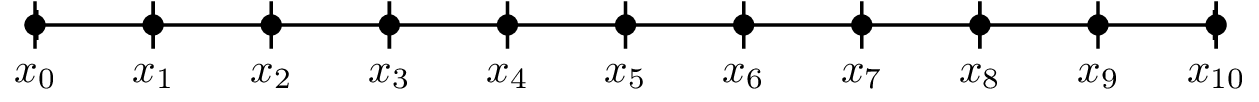
\includegraphics[width=0.6\linewidth]{images/Ch04_HeatedRod} 

}

\caption{A rod to be heated broken into 10 equal-length segments.}\label{fig:heated-rod}
\end{figure}

\begin{center}\rule{0.5\linewidth}{0.5pt}\end{center}

\begin{exercise}
\protect\hypertarget{exr:unnamed-chunk-384}{}{\label{exr:unnamed-chunk-384} }Write code to solve the following systems of equations via both LU and
QR decompositions.

\begin{enumerate}
\def\labelenumi{\alph{enumi}.}
\item
  \[\begin{array}{rl} x + 2y + 3z &= 4 \\ 2x + 4y + 3z &= 5 \\ x + y &= 4
                  \end{array}\]
\item
  \[\begin{array}{rl} 2y + 3z &= 4 \\ 2x + 3z &= 5 \\ y &= 4
                  \end{array}\]
\item
  \[\begin{array}{rl} 2y + 3z &= 4 \\ 2x + 4y + 3z &= 5 \\ x+y &= 4
                  \end{array}\]
\end{enumerate}
\end{exercise}

\begin{center}\rule{0.5\linewidth}{0.5pt}\end{center}

\begin{exercise}
\protect\hypertarget{exr:unnamed-chunk-385}{}{\label{exr:unnamed-chunk-385} }Give a specific example of a nonzero matrix which will NOT have an \(LU\) decomposition. Give specific reasons why \(LU\) will fail on your matrix.
\end{exercise}

\begin{center}\rule{0.5\linewidth}{0.5pt}\end{center}

\begin{exercise}
\protect\hypertarget{exr:unnamed-chunk-386}{}{\label{exr:unnamed-chunk-386} }Give a specific example of a nonzero matrix which will NOT have an \(QR\) decomposition. Give specific reasons why \(QR\) will fail on your matrix.
\end{exercise}

\begin{center}\rule{0.5\linewidth}{0.5pt}\end{center}

\begin{exercise}
\protect\hypertarget{exr:unnamed-chunk-387}{}{\label{exr:unnamed-chunk-387} }Have you ever wondered how scientific software computes a determinant? The formula that you learned for \href{https://en.wikipedia.org/wiki/Determinant}{calculating determinants by hand} is horribly cumbersome and computationally intractible for large matrices. This problem is meant to give you glimpse of what is \emph{actually} going on under the hood.\footnote{Actually, the determinant computation uses LU with partial pivoting which we did not cover here in the text. What we are looking at in this exercise is a smaller subcase of what happens when you have a matrix \(A\) that does not require any row swaps in the row reduction process.}

If \(A\) has an \(LU\) decomposition then \(A = LU\). Use properties that you know about determinants to come up with a simple way to find the determinant for matrices that have an \(LU\) decomposition. Show all of your work in developing your formula.

Once you have your formula for calculating \(\det(A)\), write a Python function that accepts a matrix, produces the \(LU\) decomposition, and returns the determinant of \(A\). Check your work against Python's \texttt{np.linalg.det()} function.
\end{exercise}

\begin{center}\rule{0.5\linewidth}{0.5pt}\end{center}

\begin{exercise}
\protect\hypertarget{exr:lu-error}{}{\label{exr:lu-error} }For this problem we are going to run a numerical experiment to see how the process of solving the equation \(A \boldsymbol{x} = \boldsymbol{b}\) using the \(LU\) factorization performs on random coefficient matrices \(A\) and random right-hand sides \(\boldsymbol{b}\). We will compare against Python's algorithm for solving linear systems.

We will do the following:

Create a loop that does the following:

\begin{enumerate}
\def\labelenumi{\alph{enumi}.}
\tightlist
\item
  Loop over the size of the matrix \(n\).
\item
  Build a random matrix \(A\) of size \(n \times n\). You can do this with the code \texttt{A\ =\ np.random.randn(n,n)}
\item
  Build a random vector \(\boldsymbol{b}\) in \(\mathbb{R}^{n}\). You can do this with the code \texttt{b\ =\ np.random.randn(n,1)}
\item
  Find Python's answer to the problem \(A\boldsymbol{x}=\boldsymbol{b}\) =0 using the command \texttt{exact\ =\ np.linalg.solve(A,b)}
\item
  Write code that uses your three \(LU\) functions (\texttt{myLU}, \texttt{lsolve}, \texttt{usolve}) to find a solution to the equation \(A\boldsymbol{x}=\boldsymbol{b}\).
\item
  Find the error between your answer and the exact answer using the code \texttt{np.linalg.norm(x\ -\ exact)}
\item
  Make a plot (\texttt{plt.semilogy()}) that shows how the error behaves as the size of the problem changes. You should run this for matrices of larger and larger size but be warned that the loop will run for quite a long time if you go above \(300 \times 300\) matrices. Just be patient.
\end{enumerate}

\textbf{Conclusions:} What do you notice in your final plot. What does this tell you about the behavior of our \(LU\) decomposition code?
\end{exercise}

\begin{center}\rule{0.5\linewidth}{0.5pt}\end{center}

\begin{exercise}
\protect\hypertarget{exr:unnamed-chunk-388}{}{\label{exr:unnamed-chunk-388} }Repeat Exercise \ref{exr:lu-error} for the \(QR\) decomposition. Your final plot should show both the behavior of \(QR\) and of \(LU\) throughout the experiement. What do you notice?
\end{exercise}

\begin{center}\rule{0.5\linewidth}{0.5pt}\end{center}

\begin{exercise}
\protect\hypertarget{exr:unnamed-chunk-389}{}{\label{exr:unnamed-chunk-389} }Find a least squares solution to the equation \(A \boldsymbol{x} = \boldsymbol{b}\) in two
different ways with
\[A = \begin{pmatrix} 1 & 3 & 5 \\ 4 & -2 & 6 \\ 4 & 7 & 8 \\ 3 & 7 & 19
        \end{pmatrix} \quad \text{and} \quad \boldsymbol{b} = \begin{pmatrix} 5 \\ 2 \\ -2 \\
        8\end{pmatrix}.\]
\end{exercise}

\begin{center}\rule{0.5\linewidth}{0.5pt}\end{center}

\begin{exercise}
\protect\hypertarget{exr:unnamed-chunk-390}{}{\label{exr:unnamed-chunk-390} }Let \(A\) be defined as
\[ A = \begin{pmatrix} 10^{-15} & 1 \\ 1 & 1 \end{pmatrix} \]
and let \(\boldsymbol{b}\) be the vector
\[ \boldsymbol{b}=\begin{pmatrix} 2 \\ 3\end{pmatrix}. \]\\
Notice that \(A\) has a tiny, but nonzero, value in the first entry.

\begin{enumerate}
\def\labelenumi{\alph{enumi}.}
\tightlist
\item
  Solve the linear system \(A \boldsymbol{x}=\boldsymbol{b}\) by hand.\\
\item
  Use your \texttt{myLU}, \texttt{lsolve}, and \texttt{usolve} functions to solve this problem using the LU decomposition method.\\
\item
  Compare your answers to parts (a) and (b). What went wrong?
\end{enumerate}
\end{exercise}

\begin{center}\rule{0.5\linewidth}{0.5pt}\end{center}

\begin{exercise}[Hilbert Matrices]
\protect\hypertarget{exr:unnamed-chunk-391}{}{\label{exr:unnamed-chunk-391} \iffalse (Hilbert Matrices) \fi{} }A Hilbert Matrix is a matrix of the form \(H_{ij} = 1 / (i+j-1)\). For example, a \(4 \times 4\) Hilbert Matrix is
\[ H = \begin{pmatrix} 1 & \frac{1}{2} & \frac{1}{3} & \frac{1}{4} \\
                       \frac{1}{2} & \frac{1}{3} & \frac{1}{4} & \frac{1}{5} \\ 
                       \frac{1}{3} & \frac{1}{4} & \frac{1}{5} & \frac{1}{6} \\ 
                       \frac{1}{4} & \frac{1}{5} & \frac{1}{6} & \frac{1}{7} \end{pmatrix}. \]
This type of matrix is often used to test numerical linear algebra algorithms since it is known to have some \emph{odd} behaviors \ldots{} which you'll see in a moment.

\begin{enumerate}
\def\labelenumi{\alph{enumi}.}
\tightlist
\item
  Write code to build a \(n\times n\) Hilbert Matrix and call this matrix \(H\). Test your code for various values of \(n\) to be sure that it is building the correct matrices.
\item
  Build a vector of ones called \(\boldsymbol{b}\) with code \texttt{b\ =\ np.ones(\ (n,1)\ )}. We will use \(\boldsymbol{b}\) as the right hand side of the system of equations \(H\boldsymbol{x} = \boldsymbol{b}\).
\item
  Solve the system of equations \(H \boldsymbol{x} = \boldsymbol{b}\) using any technique you like from this chapter.
\item
  Now let's say that you change the first entry of \(\boldsymbol{b}\) by just a little bit, say 10\^{}(-15). If we were to now solve the equation \(H \boldsymbol{x}_{new} = \boldsymbol{b}_{new}\) what would you expect as compared to solving \(H \boldsymbol{x} = \boldsymbol{b}\).
\item
  Now let's actually make the change suggested in part (d). Use the code \texttt{bnew\ =\ np.ones(\ (n,1)\ )} and then \texttt{bnew{[}0{]}\ =\ bnew{[}0{]}\ +\ 1e-15} to build a new \(\boldsymbol{b}\) vector with this small change. Solve \(H\boldsymbol{x}=\boldsymbol{b}\) and \(H\boldsymbol{x}_{new}=\boldsymbol{b}_{new}\) and then compare the maximum absolute difference \texttt{np.max(\ np.abs(\ x\ -\ xnew\ )\ )}. What do you notice? Make a plot with \(n\) on the horizontal axis and the maximum absolute difference on the vertical axis. What does this plot tell you about the solution to the equation \(H \boldsymbol{x} = \boldsymbol{b}\)?
\item
  We know that \(H H^{-1}\) should be the identity matrix. As we'll see, however, Hilbert matrices are particularly poorly behaved! Write a loop over \(n\) that (i) builds a Hilbert matrix of size \(n\), (ii) calculates \(H * H^{-1}\) (using \texttt{np.linalg.inv()} to compute the inverse directly), (iii) calculates the norm of the difference between the identity matrix (\texttt{np.identity(n)}) and your calculated identity matrix from part (ii). Finally. Build a plot that shows \(n\) on the horizontal axis and the normed difference on the vertical axis. What do you see? What does this mean about the matrix inversion of the Hilbert matrix.
\item
  There are cautionary tales hiding in this problem. Write a paragraph explaining what you can learn by playing with pathological matrices like the Hilbert Matrix.
\end{enumerate}
\end{exercise}

\begin{center}\rule{0.5\linewidth}{0.5pt}\end{center}

\begin{exercise}
\protect\hypertarget{exr:unnamed-chunk-392}{}{\label{exr:unnamed-chunk-392} }Now that you have \(QR\) and \(LU\) code we're going to use both of them! The problem is as follows:\\
We are going to find the polynomial of degree 4 that best fits the function
\$\[ y = \cos(4t) + 0.1 \varepsilon(t) \]
at 50 equally spaced points \(t\) between \(0\) and \(1\). Here we are using \(\varepsilon(t)\) as a function that outputs normally distributed random white noise. In Python you will build \(y\) as \texttt{y\ =\ np.cos(4*t)\ +\ 0.1*np.random.randn(t.shape)}

Build the \(t\) vector and the \(y\) vector (these are your data). We need to set up the least squares problems \(A \boldsymbol{x} = \boldsymbol{b}\) by setting up the matrix \(A\) as we did in the other least squares curve fitting problems and by setting up the \(\boldsymbol{b}\) vector using the \(y\) data you just built.

\begin{enumerate}
\def\labelenumi{\alph{enumi}.}
\tightlist
\item
  Solve the normal equations \(A^T A \boldsymbol{x} = A^T \boldsymbol{b}\) using your \(LU\) code.
\item
  Solve the system \(A \boldsymbol{x} = \boldsymbol{b}\) by first transforming \(A\) to \(A = QR\) and then solving \(R\boldsymbol{x} = Q^T \boldsymbol{b}\).
\item
  Use Python to find the sum of the square errors between the polynomial approximation and the function \(f(t) = \cos(4t)\) for both the \(QR\) and the \(LU\) approaches.
\item
  Build code that does parts (a) - (c) several hundred times and complies results comparing which method gives the better approximation (smaller sum of square error). Give appropriate plots of your results. What conclusions can you make in general?
\end{enumerate}
\end{exercise}

\begin{center}\rule{0.5\linewidth}{0.5pt}\end{center}

\begin{exercise}
\protect\hypertarget{exr:unnamed-chunk-393}{}{\label{exr:unnamed-chunk-393} }Find the largest eigenvalue of the matrix \(A\) WITHOUT using any built-in Python command for finding eigenstructure.
\[A = \begin{pmatrix} 1 & 2 & 3 & 4 \\ 5 & 6 & 7 & 8 \\ 9 & 0 & 1 & 2 \\ 3 & 4 & 5 &
        6 \end{pmatrix}\]
\end{exercise}

\begin{center}\rule{0.5\linewidth}{0.5pt}\end{center}

\begin{exercise}
\protect\hypertarget{exr:unnamed-chunk-394}{}{\label{exr:unnamed-chunk-394} }It is possible in a matrix that the eigenvalues \(\lambda_1\) and \(\lambda_2\) are equal but with the corresponding eigenvectors not equal. Before you experiment with matrices of this sort, write a conjecture about what will happen to the power method in this case (look back to our proof in Exercise \ref{exr:power-proof} of how the power method works). Now build several specific matrices where this is the case and see what happens to the power method.
\end{exercise}

\begin{center}\rule{0.5\linewidth}{0.5pt}\end{center}

\begin{exercise}
\protect\hypertarget{exr:unnamed-chunk-395}{}{\label{exr:unnamed-chunk-395} }Will the power method fail, slow down, or be uneffected if one (or more) of the non-dominant eigenvalues is zero? Give sufficient mathematical evidence or show several numerical experiments to support your answer.
\end{exercise}

\begin{center}\rule{0.5\linewidth}{0.5pt}\end{center}

\begin{exercise}
\protect\hypertarget{exr:unnamed-chunk-396}{}{\label{exr:unnamed-chunk-396} }Find a cubic function that best fits the following data.
\end{exercise}

\begin{longtable}[]{@{}ll@{}}
\toprule
\(x\) Data & \(y\) Data\tabularnewline
\midrule
\endhead
0 & 1.0220\tabularnewline
0.0500 & 1.0174\tabularnewline
0.1000 & 1.0428\tabularnewline
0.1500 & 1.0690\tabularnewline
0.2000 & 1.0505\tabularnewline
0.2500 & 1.0631\tabularnewline
0.3000 & 1.0458\tabularnewline
0.3500 & 1.0513\tabularnewline
0.4000 & 1.0199\tabularnewline
0.4500 & 1.0180\tabularnewline
0.5000 & 1.0156\tabularnewline
0.5500 & 0.9817\tabularnewline
0.6000 & 0.9652\tabularnewline
0.6500 & 0.9429\tabularnewline
0.7000 & 0.9393\tabularnewline
0.7500 & 0.9266\tabularnewline
0.8000 & 0.8959\tabularnewline
0.8500 & 0.9014\tabularnewline
0.9000 & 0.8990\tabularnewline
0.9500 & 0.9038\tabularnewline
1.0000 & 0.8989\tabularnewline
\bottomrule
\end{longtable}

\begin{center}\rule{0.5\linewidth}{0.5pt}\end{center}

\begin{theorem}
\protect\hypertarget{thm:symmetric-eigenvalues}{}{\label{thm:symmetric-eigenvalues} }If \(A\) is a symmetric matrix with eigenvalues \(\lambda_1, \lambda_2, \ldots, \lambda_n\) then \(|\lambda_1| > |\lambda_2| > \cdots > |\lambda_n|\). Furthermore, the eigenvectors will be orthogonal to each other.
\end{theorem}

\begin{exercise}[The Deflation Method]
\protect\hypertarget{exr:unnamed-chunk-397}{}{\label{exr:unnamed-chunk-397} \iffalse (The Deflation Method) \fi{} }
For symmetric matrices we can build an extension to the power method in order to find the second most dominant eigen-pair for a matrix \(A\). Theorem \ref{thm:symmetric-eigenvalues} suggests the following method for finding the second dominant eigen-pair for a symmetric matrix. This method is called the \textbf{deflation method}.

\begin{itemize}
\tightlist
\item
  Use the power method to find the dominant eigenvalue and eigenvector.
\item
  Start with a random unit vector of the correct shape.
\item
  Multiplying your vector by \(A\) will \emph{pull it toward} the dominant eigenvector. After you multiply, project your vector onto the dominant eigenvector and find the projection error.
\item
  Use the projection error as the new approximation for the eigenvector (Why should we do this? What are we really finding here?)
\end{itemize}

Note that the deflation method is really exactly the same as the power method with the exception that we orthogonalize at every step. Hence, when you write your code expect to only change a few lines from your power method.

Write a function to find the second largest eigenvalue and eigenvector pair by putting the deflation method into practice. Test your code on a matrix \(A\) and compare against Python's \texttt{np.linalg.eig()} command. Your code needs to work on symmetric matrices of arbitrary size and you need to write test code that clearly shows the error between your calculated eigenvalue and Python's eigenvalue as well as your calculated eigenvector and 's eigenvector.

To guarantee that you start with a symmetric matrix you can use the
following code.
\end{exercise}

\begin{Shaded}
\begin{Highlighting}[]
\ImportTok{import}\NormalTok{ numpy }\ImportTok{as}\NormalTok{ np}
\NormalTok{N }\OperatorTok{=} \DecValTok{40}
\NormalTok{A }\OperatorTok{=}\NormalTok{ np.random.randn(N,N)}
\NormalTok{A }\OperatorTok{=}\NormalTok{ np.matrix(A)}
\NormalTok{A }\OperatorTok{=}\NormalTok{ np.transpose(A) }\OperatorTok{*}\NormalTok{ A }\CommentTok{\# this should build a symmetric matrix (why?)}
\end{Highlighting}
\end{Shaded}

\begin{center}\rule{0.5\linewidth}{0.5pt}\end{center}

\begin{exercise}
\protect\hypertarget{exr:unnamed-chunk-399}{}{\label{exr:unnamed-chunk-399} }(This concept for this problem is modified from {[}\protect\hyperlink{ref-meerschaert}{6}{]}. The data is taken from \href{https://www.weather.gov/arx/mississippi_river}{NOAA and the National Weather Service} with the specific values associated with La Crosse, WI.)

Floods in the Mississippi River Valleys of the upper midwest have somewhat predictable day-to-day behavior in that the flood stage today has high predictive power for the flood stage tomorrow. Assume that the flood stages are:

\begin{itemize}
\tightlist
\item
  Stage 0 (Normal): Average daily flow is below 90,000 \(ft^3/sec\) (cubic feet per second = cfs). This is the \emph{normal} river level.
\item
  Stage 1 (Action Level): Average daily flow is between 90,000 cfs and 124,000 cfs.
\item
  Stage 2 (Minor Flood): Average daily flow is between 124,000 cfs and 146,000 cfs.
\item
  Stage 3 (Moderate Flood): Average daily flow is between 146,000 cfs and 170,000 cfs.
\item
  Stage 4 (Extreme Flood): Average daily flow is above 170,000 cfs.
\end{itemize}

The following table shows the probability of one stage transitioning into another stage from one day to the next.

\begin{longtable}[]{@{}llllll@{}}
\toprule
& Stage 0 Today & Stage 1 Today & Stage 2 Today & Stage 3 Today & Stage 4 Today\tabularnewline
\midrule
\endhead
Stage 0 Tomorrow & 0.9 & 0.3 & 0 & 0 & 0\tabularnewline
Stage 1 Tomorrow & 0.05 & 0.7 & 0.4 & 0 & 0\tabularnewline
Stage 2 Tomorrow & 0.025 & 0 & 0.6 & 0.6 & 0\tabularnewline
Stage 3 Tomorrow & 0.015 & 0 & 0 & 0.4 & 0.8\tabularnewline
Stage 4 Tomorrow & 0.01 & 0 & 0 & 0 & 0.2\tabularnewline
\bottomrule
\end{longtable}

Mathematically, if \(\boldsymbol{s}_k\) is the state at day \(k\) and \(A\) is the matrix given in the table above then the difference equation \(\boldsymbol{s}_{k+1} = A \boldsymbol{s}_k\) shows how a state will transition from day to day. For example, if we are currently in Stage 0 then \[ \boldsymbol{s}_0 = \begin{pmatrix} 1 \\ 0 \\ 0 \\ 0 \\ 0 \end{pmatrix}. \]
We can interpret this as ``\emph{there is a probability of 1 that we are in Stage 0 today and there is a probability of 0 that we are in any other stage today.}''

If we want to advance this model forward in time then we just need to iterate. In our example, the state tomorrow would be \(\boldsymbol{s}_1 = A \boldsymbol{s}_0\). The state two days from now would be \(\boldsymbol{s}_2 = A \boldsymbol{s}_1\), and if we use the expression for \(\boldsymbol{s}_1\) we can simplify to \(\boldsymbol{s}_2 = A^2 \boldsymbol{s}_0\).

\begin{enumerate}
\def\labelenumi{\alph{enumi}.}
\tightlist
\item
  Prove that the state at day \(n\) is \(\boldsymbol{s}_n = A^n \boldsymbol{s}_0\).
\item
  If \(n\) is large then the steady state solution to the difference equation in part (a) is given exactly by the power method iteration that we have studied in this chapter. Hence, as the iterations proceed they will be pulled toward the dominant eigenvector. Use the power method to find the dominant eigenvector of the matrix \(A\).\\
\item
  The vectors in this problem are called \textbf{probability vectors} in the sense that the vectors sum to 1 and every entry can be interpreted as a probability. Re-scale your answer from part (b) so that we can interpret the entries as probabilities. That is, ensure that the sum of the vector from part (b) is 1.\\
\item
  Interpret your answer to part (c) in the context of the problem. Be sure that your interpretation could be well understood by someone that does not know the mathematics that you just did.
\end{enumerate}
\end{exercise}

\begin{center}\rule{0.5\linewidth}{0.5pt}\end{center}

\hypertarget{projects-2}{%
\section{Projects}\label{projects-2}}

In this section we propose several ideas for projects related to
numerical linear algebra. These projects are meant to be open ended, to
encourage creative mathematics, to push your coding skills, and to
require you to write and communicate your mathematics. Take the time to
read Appendix \ref{ch:writing} before you write your final solution.

\hypertarget{the-google-page-rank-algorithm}{%
\subsection{The Google Page Rank Algorithm}\label{the-google-page-rank-algorithm}}

In this project you will discover how the Page Rank algorithm works to
give the most relevant information as the top hit on a Google search.

Search engines compile large indexes of the dynamic information on the
Internet so they are easily searched. This means that when you do a
Google search, you are not actually searching the Internet; instead, you
are searching the indexes at Google.

When you type a query into Google the following two steps take place:

\begin{enumerate}
\def\labelenumi{\arabic{enumi}.}
\item
  Query Module: The query module at Google converts your natural
  language into a language that the search system can understand and
  consults the various indexes at Google in order to answer the query.
  This is done to find the list of relevant pages.
\item
  Ranking Module: The ranking module takes the set of relevant pages
  and ranks them. The outcome of the ranking is an ordered list of web
  pages such that the pages near the top of the list are most likely
  to be what you desire from your search. This ranking is the same as
  assigning a \emph{popularity score} to each web site and then listing the
  relevant sites by this score.
\end{enumerate}

This section focuses on the Linear Algebra behind the Ranking Module
developed by the founders of Google: Sergey Brin and Larry Page. Their
algorithm is called the \emph{Page Rank algorithm}, and you use it every
single time you use Google's search engine.

In simple terms: \emph{A webpage is important if it is pointed to by other
important pages}.

The Internet can be viewed as a directed graph (look up this term \href{https://en.wikipedia.org/wiki/Directed_graph}{here
on Wikipedia}) where the
nodes are the web pages and the edges are the hyperlinks between the
pages. The hyperlinks into a page are called \emph{in links}, and the ones
pointing out of a page are called \emph{out links}. In essence, a hyperlink
from my page to yours is my endorsement of your page. Thus, a page with
more recommendations must be more important than a page with a few
links. However, the status of the recommendation is also important.

Let us now translate this into mathematics. To help understand this we
first consider the small web of six pages shown in Figure
\ref{fig:example-graph} (a graph of the router level of the
internet can be found
\href{https://personalpages.manchester.ac.uk/staff/m.dodge/cybergeography/atlas/lumeta_large.jpg}{here}).
The links between the pages are shown by arrows. An arrow pointing into
a node is an \emph{in link} and an arrow pointing out of a node is an
\emph{out link}. In Figure \ref{fig:example-graph}, node 3 has three out links (to nodes 1,
2, and 5) and 1 in link (from node 1).

\begin{figure}

{\centering 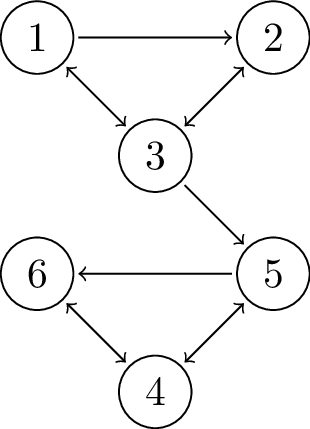
\includegraphics[width=0.2\linewidth]{images/Ch04_GoogleGraph1} 

}

\caption{Example web graph.}\label{fig:example-graph}
\end{figure}

We will first define some notation in the Page Rank algorithm:

\begin{itemize}
\item
  \(|P_i|\) is the number of out links from page \(P_i\)
\item
  \(H\) is the \emph{hyperlink} matrix defined as
  \[H_{ij} = \left\{ \begin{array}{cl} \frac{1}{|P_j|}, & \text{if there is a link
              from node $j$ to node $i$} \\ 0, & \text{otherwise} \end{array} \right.\]
  where the ``\(i\)'' and ``\(j\)'' are the row and column indices
  respectively.
\item
  \(\boldsymbol{x}\) is a vector that contains all of the Page Ranks for the
  individual pages.
\end{itemize}

The Page Rank algorithm works as follows:

\begin{enumerate}
\def\labelenumi{\arabic{enumi}.}
\item
  Initialize the page ranks to all be equal. This means that our
  initial assumption is that all pages are of equal rank. In the case
  of Figure \ref{fig:example-graph} we would take \(\boldsymbol{x}_0\) to be
  \[\boldsymbol{x}_0 = \begin{pmatrix} 1/6 \\ 1/6 \\ 1/6 \\ 1/6 \\ 1/6 \\ 1/6 \end{pmatrix}.\]
\item
  Build the hyperlink matrix.\\
  As an example we'll consider node 3 in Figure \ref{fig:example-graph}. There are three out links from node 3
  (to nodes 1, 2, and 5). Hence \(H_{13}=1/3\), \(H_{23} = 1/3\), and
  \(H_{53} = 1/3\) and the partially complete hyperlink matrix is
  \[H = \begin{pmatrix} 
                  - & - & 1/3 & - & - & - \\
                  - & - & 1/3 & - & - & - \\
                  - & - & 0   & - & - & - \\
                  - & - & 0   & - & - & - \\
                  - & - & 1/3 & - & - & - \\
                  - & - & 0   & - & - & - 
              \end{pmatrix}\]
\item
  The difference equation \(\boldsymbol{x}_{n+1} = H \boldsymbol{x}_n\) is used to iteratively
  refine the estimates of the page ranks. You can view the iterations
  as a person visiting a page and then following a link at random,
  then following a random link on the next page, and the next, and the
  next, etc. Hence we see that the iterations evolve exactly as
  expected for a difference equation.
\end{enumerate}

\begin{longtable}[]{@{}ll@{}}
\toprule
Iteration & New Page Rank Estimation\tabularnewline
\midrule
\endhead
0 & \(\boldsymbol{x}_0\)\tabularnewline
1 & \(\boldsymbol{x}_1 = H \boldsymbol{x}_0\)\tabularnewline
2 & \(\boldsymbol{x}_2 = H \boldsymbol{x}_1 = H^2 \boldsymbol{x}_0\)\tabularnewline
3 & \(\boldsymbol{x}_3 = H \boldsymbol{x}_2 = H^3 \boldsymbol{x}_0\)\tabularnewline
4 & \(\boldsymbol{x}_4 = H \boldsymbol{x}_3 = H^4 \boldsymbol{x}_0\)\tabularnewline
\(\vdots\) & \(\vdots\)\tabularnewline
\(k\) & \(\boldsymbol{x}_k = H^k \boldsymbol{x}_0\)\tabularnewline
\bottomrule
\end{longtable}

\begin{enumerate}
\def\labelenumi{\arabic{enumi}.}
\setcounter{enumi}{3}
\tightlist
\item
  When a steady state is reached we sort the resulting vector \(\boldsymbol{x}_k\)
  to give the page rank. The node (web page) with the highest rank
  will be the top search result, the second highest rank will be the
  second search result, and so on.
\end{enumerate}

It doesn't take much to see that this process can be very time
consuming. Think about your typical web search with hundreds of
thousands of hits; that makes a square matrix \(H\) that has a size of
hundreds of thousands of entries by hundreds of thousands of entries!
The matrix multiplications alone would take many minutes (or possibly
many hours) for every search! \ldots but Brin and Page were pretty smart
dudes!!

We now state a few theorems and definitions that will help us simplify
the iterative Page Rank process.

\begin{center}\rule{0.5\linewidth}{0.5pt}\end{center}

\begin{theorem}
\protect\hypertarget{thm:eigen-expand}{}{\label{thm:eigen-expand} }If
\(A\) is an \(n \times n\) matrix with \(n\) linearly independent eigenvectors
\(\boldsymbol{v}_1,  \boldsymbol{v}_2, \boldsymbol{v}_3,\) \(\ldots, \boldsymbol{v}_n\) and associated eigenvalues
\(\lambda_1, \lambda_2,  \lambda_3, \ldots, \lambda_n\) then for any initial vector
\(\boldsymbol{x} \in \mathbb{R}^n\) we can write \(A^k \boldsymbol{x}\) as
\[A^k \boldsymbol{x} = c_1 \lambda_1^k \boldsymbol{v}_1 + c_2 \lambda_2^k \boldsymbol{v}_2 + c_3 \lambda_3^k \boldsymbol{v}_3 +
        \cdots c_n \lambda_n^k \boldsymbol{v}_n\] where
\(c_1, c_2, c_3, \ldots, c_n\) are the constants found by expressing \(\boldsymbol{x}\)
as a linear combination of the eigenvectors.\\
Note: We can assume that the eigenvalues are ordered such that
\(|\lambda_1| > |\lambda_2| \ge |\lambda_3| \ge \cdots \ge |\lambda_n|\).
\end{theorem}

\begin{center}\rule{0.5\linewidth}{0.5pt}\end{center}

\begin{exercise}
\protect\hypertarget{exr:unnamed-chunk-400}{}{\label{exr:unnamed-chunk-400} }Prove the preceding theorem.
\end{exercise}

\begin{center}\rule{0.5\linewidth}{0.5pt}\end{center}

A \textbf{probability vector} is a vector with entries on the interval
\([0,1]\) that add up to 1.

A \textbf{stochastic matrix} is a square matrix whose columns are probability
vectors.

\begin{center}\rule{0.5\linewidth}{0.5pt}\end{center}

\begin{theorem}
\protect\hypertarget{thm:largest-ev-stochastic}{}{\label{thm:largest-ev-stochastic} }If \(A\) is a stochastic \(n \times n\)
matrix then \(A\) will have \(n\) linearly independent eigenvectors.
Furthermore, the largest eigenvalue of a stochastic matrix will be
\(\lambda_1 = 1\) and the smallest eigenvalue will always be nonnegative:
\(0 \le |\lambda_n| < 1\).
\end{theorem}

Some of the following tasks will ask you to \emph{prove} a statement or a
theorem. This means to clearly write all of the logical and mathematical
reasons why the statement is true. Your proof should be absolutely
crystal clear to anyone with a similar mathematical background \ldots if you
are in doubt then have a peer from a different group read your proof to
you .

\begin{center}\rule{0.5\linewidth}{0.5pt}\end{center}

\begin{exercise}
\protect\hypertarget{exr:unnamed-chunk-401}{}{\label{exr:unnamed-chunk-401} }Finish writing the hyperlink matrix \(H\) from Figure \ref{fig:example-graph}.
\end{exercise}

\begin{center}\rule{0.5\linewidth}{0.5pt}\end{center}

\begin{exercise}
\protect\hypertarget{exr:unnamed-chunk-402}{}{\label{exr:unnamed-chunk-402} }Write code to implement the iterative process defined previously. Make a
plot that shows how the rank evolves over the iterations.
\end{exercise}

\begin{center}\rule{0.5\linewidth}{0.5pt}\end{center}

\begin{exercise}
\protect\hypertarget{exr:unnamed-chunk-403}{}{\label{exr:unnamed-chunk-403} }What must be true about a collection of \(n\) pages such that an
\(n\times n\) hyperlink matrix \(H\) is a stochastic matrix.
\end{exercise}

\begin{center}\rule{0.5\linewidth}{0.5pt}\end{center}

\begin{exercise}
\protect\hypertarget{exr:unnamed-chunk-404}{}{\label{exr:unnamed-chunk-404} }The statement of the next theorem is incomplete, but the proof is given
to you. Fill in the blank in the statement of the theorem and provide a
few sentences supporting your answer.
\end{exercise}

\begin{center}\rule{0.5\linewidth}{0.5pt}\end{center}

\begin{theorem}
\protect\hypertarget{thm:steady}{}{\label{thm:steady} }If \(A\) is an
\(n \times n\) stochastic matrix and \(\boldsymbol{x}_0\) is some initial vector for
the difference equation \(\boldsymbol{x}_{n+1} = A \boldsymbol{x}_n\), then the steady state
vector is
\[\boldsymbol{x}_{equilib} = \lim_{k \to\infty} A^k \boldsymbol{x}_0 = \underline{\hspace{1in}}.\]
\end{theorem}

\textbf{Proof:}

First note that \(A\) is an \(n \times n\) stochastic matrix so from Theorem \ref{thm:largest-ev-stochastic} we know that there are \(n\)
linearly independent eigenvectors. We can then substitute the
eigenvalues from Theorem \ref{thm:largest-ev-stochastic} in Theorem \ref{thm:eigen-expand}. Noting that if \(0<\lambda_j<1\) we have
\(\lim_{k \to  \infty} \lambda_j^k = 0\) the result follows immediately.

\begin{center}\rule{0.5\linewidth}{0.5pt}\end{center}

\begin{exercise}
\protect\hypertarget{exr:unnamed-chunk-405}{}{\label{exr:unnamed-chunk-405} }Discuss how Theorem \ref{thm:steady} greatly simplifies the PageRank iterative
process described previously. In other words: there is no reason to
iterate at all. Instead, just find \ldots{} what?
\end{exercise}

\begin{center}\rule{0.5\linewidth}{0.5pt}\end{center}

\begin{exercise}
\protect\hypertarget{exr:unnamed-chunk-406}{}{\label{exr:unnamed-chunk-406} }Now use the previous two problems to find the resulting PageRank vector
from the web in Figure \ref{fig:example-graph}? Be sure to rank the pages in order of
importance. Compare your answer to the one that you got in problem 2.
\end{exercise}

\begin{center}\rule{0.5\linewidth}{0.5pt}\end{center}

\begin{figure}

{\centering 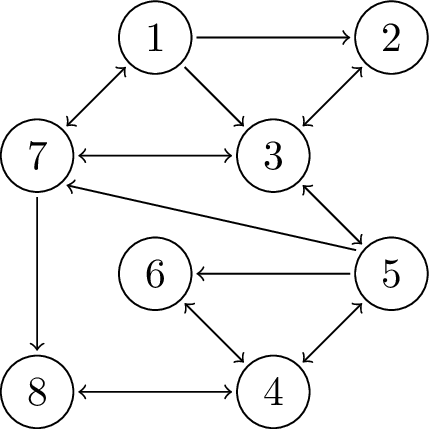
\includegraphics[width=0.3\linewidth]{images/Ch04_GoogleGraph2} 

}

\caption{A second example web graph.}\label{fig:graph2}
\end{figure}

\begin{exercise}
\protect\hypertarget{exr:unnamed-chunk-407}{}{\label{exr:unnamed-chunk-407} }Consider the web in Figure \ref{fig:graph2}.

\begin{enumerate}
\def\labelenumi{\arabic{enumi}.}
\item
  Write the \(H\) matrix and find the initial state \(\boldsymbol{x}_0\),
\item
  Find steady state PageRank vector using the two different methods
  described: one using the iterative difference equation and the other
  using Theorem \ref{thm:steady} and the dominant eigenvector.
\item
  Rank the pages in order of importance.
\end{enumerate}
\end{exercise}

\begin{center}\rule{0.5\linewidth}{0.5pt}\end{center}

\begin{exercise}
\protect\hypertarget{exr:unnamed-chunk-408}{}{\label{exr:unnamed-chunk-408} }One thing that we didn't consider in this version of the Google Page
Rank algorithm is the random behavior of humans. One, admittedly
slightly naive, modification that we can make to the present algorithm
is to assume that the person surfing the web will randomly jump to any
other page in the web at any time. For example, if someone is on page 1
in Figure \ref{fig:graph2} then they could randomly jump to any page 2 - 8.
They also have links to pages 2, 3, and 7. That is a total of 10
possible next steps for the web surfer. There is a \(2/10\) chance of
heading to page 2. One of those is following the link from page 1 to
page 2 and the other is a random jump to page 2 without following the
link. Similarly, there is a \(2/10\) chance of heading to page 3, \(2/10\)
chance of heading to page 7, and a \(1/10\) chance of randomly heading to
any other page.

Implement this new algorithm, called the \emph{random surfer algorithm}, on
the web in Figure \ref{fig:graph2}. Compare your ranking to the non-random surfer
results from the previous problem.
\end{exercise}

\begin{center}\rule{0.5\linewidth}{0.5pt}\end{center}

\hypertarget{ch:odes}{%
\chapter{Ordinary Differential Equations}\label{ch:odes}}

\hypertarget{intro-to-numerical-odes}{%
\section{Intro to Numerical ODEs}\label{intro-to-numerical-odes}}

\begin{quote}
\emph{``The mathematical discipline of differential equations furnishes the
explanation of all those elementary manifestations of nature which
involve time.''}\\
--\href{https://en.wikipedia.org/wiki/Sophus_Lie}{Norwegian Mathematician Sophus
Lie}
\end{quote}

Ordinary Differential Equations (ODEs) arise in all manner of contexts, but the most prevalent and frequently cited are from physics and engineering. The applications of Newton's Second Law, for example, give differential equations relating position, velocity, and acceleration. Newton's second law is the equation \(F = ma\) where \(F\) is a force acting on a body, \(m\) is the mass of the body, and \(a\) is the acceleration. From Calculus recall that \(a = v' = s''\), so Newton's second law can be rephrased as \(F = mv'\), a differential equation with velocity as the unknown, or \(F = ms''\), a second order differential equation with position as the unknown. Some of the cases where we use Newton's second law have nice analytic solutions, such as the motion of an object on a frictionless surface under constant force. However, many of these cases are highly idealized and not reflective of true reality. It doesn't take much to cause the differential equation(s) resulting from Newton's second law to be terribly hard, or maybe impossible, to solve. Just add some friction, perhaps allow multiple bodies to interact, or consider the forces that act differently on multiple length scales. A famous example is the \href{https://en.wikipedia.org/wiki/Three-body_problem}{three body problem} where gravitational forces drive the motion of three celestial bodies. The resulting differential equations have no analytic solution and the only way to show how the positions of the bodies evolve in time is with a numerical approximation \ldots{} And that's just 3 celestial bodies! Imagine how complicated the differential equations get trying to model our solar system (or our galaxy)!

Other examples of ODEs that are impossible to solve analytically are

\begin{itemize}
\tightlist
\item
  The motion of a pendulum where the angle from equilibrium is allowed to be large or the pendulum is allowed to swing over the top (e.g.~\href{https://en.wikipedia.org/wiki/Pendulum_(mathematics)\#Simple_gravity_pendulum}{the nonlinear pendulum}).
\item
  Systems of differential equations that model nonlinear predator-prey interactions (e.g.~\href{https://en.wikipedia.org/wiki/Lotka\%E2\%80\%93Volterra_equations}{the Lotka-Voltera equations}).
\item
  Some types of damped oscillations in electric circuits (e.g.~\href{https://en.wikipedia.org/wiki/Van_der_Pol_oscillator}{the Van der Pol oscillator}).
\item
  \ldots{} and many others.
\end{itemize}

The impossibility of solving a differential equation stems partly from the impossibility of integrating most functions. If we were to just randomly choose functions to integrate we would find that the vast majority do not have antiderivatives. The story in ODEs is the same: pick any combination of a function, its derivatives, and other forcing functions and you will find that there is no way to arrive at an analytic solution involving the regular operations and functions of mathematics: linear combinations, powers, roots, trigonometric functions, logarithms, etc. There are theorems from differential equations that will guarantee the existence and uniqueness of solutions to many differential equations, but just knowing that the solution exists isn't enough to actually go and find it. Numerical techniques give us an avenue to at least approximate these solutions.

So what \emph{is} a numerical solution to a differential equation?\\
When solving a differential equation with analytic techniques the goal is to come up with a function. In a numerical solution the goal is typically to divide the domain (typically the domain is time) for the solution function into a fine partition, just like we did with numerical differentiation and integration, and then to approximate the solution to the differential equation at each point in that partition. Hence, the end result will be a list of approximate solution values associated with each time. In the strictest sense a list of approximate solutions on a partition \emph{is} actually a function (a relation between input and output), but this isn't a function in terms of sines, powers, roots, logarithms, etc. The best way to deliver a numerical solution is just to make a plot. Your intuition of what the plot should look like based on the context of the problem is one of the best tools for you to check your work.

\begin{center}\rule{0.5\linewidth}{0.5pt}\end{center}

\begin{exercise}
\protect\hypertarget{exr:unnamed-chunk-409}{}{\label{exr:unnamed-chunk-409} }Sketch a plot of the function that would model each of the following
scenarios.

\begin{enumerate}
\def\labelenumi{\alph{enumi}.}
\item
  A population of an endangered species is slowly dying off. The rate
  at which the population decreases is proportional to the amount of
  population that is presently there. What does the population as a
  function of time look like for this species?
\item
  Consider a mass hanging from a spring that is suspended vertically from the ceiling. If the mass is given an initial upward \emph{bump} and then left alone, what will the position of the mass relative to its equilibrium state be as a function of time?
\item
  A pollutant has entered a tributary for a certain reservoir, and a
  small concentration leaks into the water over a long period of time.
  The reservoir is dam controlled so the rate of release is well known
  and relatively constant. What does the function modeling the amount
  of pollutant look like as time goes on?
\item
  A drug is eliminated from the body via natural metabolism. Assume
  that there is some initial amount of drug in the body. What does the
  function modeling the amount of drug in the system look like over
  time?
\end{enumerate}
\end{exercise}

\begin{center}\rule{0.5\linewidth}{0.5pt}\end{center}

Now let's formalize the conversation about differential equations, analytic solutions, and numerical solutions.

\begin{definition}[Differential Equation]
\protect\hypertarget{def:unnamed-chunk-410}{}{\label{def:unnamed-chunk-410} \iffalse (Differential Equation) \fi{} }A \textbf{differential equation} is an equation that relates the derivative
(or derivatives) of an unknown function to itself.
\end{definition}

\begin{center}\rule{0.5\linewidth}{0.5pt}\end{center}

\begin{definition}[Solution to a Differential Equations]
\protect\hypertarget{def:unnamed-chunk-411}{}{\label{def:unnamed-chunk-411} \iffalse (Solution to a Differential Equations) \fi{} }A \textbf{solution to a differential equation} (also called an \textbf{analytic solution}) is a function which, when substituted into the differential equation, creates a true statement.
\end{definition}

\begin{center}\rule{0.5\linewidth}{0.5pt}\end{center}

\begin{example}
\protect\hypertarget{exm:unnamed-chunk-412}{}{\label{exm:unnamed-chunk-412} }The function \(x(t) = 3e^{-0.25t}\) is a solution to the differential equation \(x' = -0.25x\) with initial condition \(x(0) = 3\). We can verify this by substituting \(x(t)\) into the differential equation:
\[\begin{aligned} 
\frac{d}{dt} \left( x(t) \right) &\stackrel{?}{=} -0.25 x(t)\\
\implies \frac{d}{dt} \left( 3e^{-0.25t} \right) &\stackrel{?}{=} -0.25 \left( 3e^{-0.25t} \right) \\
\implies -0.25 \left( 3e^{-0.25t} \right) &\stackrel{\checkmark}{=} -0.25 \left( 3e^{-0.25t} \right)
\end{aligned}
\]
Furthermore, \(x(0) = 3e^{-0.25 \cdot 0} = 3e^0 = 3 \checkmark\). Hence, the function \(x(t) = 3e^{-0.25t}\) is indeed a solution to the differential equation \(x'=-0.25x\) with \(x(0) = 3\).
\end{example}

\begin{center}\rule{0.5\linewidth}{0.5pt}\end{center}

\begin{exercise}
\protect\hypertarget{exr:unnamed-chunk-413}{}{\label{exr:unnamed-chunk-413} }A \textbf{numerical solution to a differential equation} is a list of ordered
pairs that gives a point-wise approximation to the actual solution.
\end{exercise}

\begin{center}\rule{0.5\linewidth}{0.5pt}\end{center}

In this chapter we will examine some of the more common ways to create approximations of solutions to differential equations. Moreover, we will lean heavily on Taylor Series to give us ways to accurately measure the order of the errors that we make in the process.

\hypertarget{recalling-the-basics-of-odes}{%
\section{Recalling the Basics of ODEs}\label{recalling-the-basics-of-odes}}

You should be familiar with the basics of differential equations from previous classes, but just in case you're a bit rusty, this section gives a very brief review of some of the basics.

Solving differential equations analytically is a subject unto itself, but it is worth our time here to revisit some of the basic techniques for solving differential equations. It should be noted that if an analytic solution exits then there is no reason to do any of the numerical techniques that we will discuss in this chapter -- if you have an exact analytic solution then why on earth would you then approximate the solution!? The fact of the matter is, however, that the techniques for finding analytic solutions to differential equations are rather limited relative to the wild zoo of possible ODEs, and when the differential equations get complicated we will only have numerical approximations to lean back on. However, when we build approximation methods we will test them on differential equations for which we have the answer. So let's get started with some review.

\begin{center}\rule{0.5\linewidth}{0.5pt}\end{center}

\begin{exercise}
\protect\hypertarget{exr:unnamed-chunk-414}{}{\label{exr:unnamed-chunk-414} }Identify which of the following problems are \emph{differential} equations
and which are \emph{algebraic} equations. (Do not try to solve any of these equations)

\begin{enumerate}
\def\labelenumi{\alph{enumi}.}
\tightlist
\item
  \(x^2 + 5x = 7x^3 - 2\)
\item
  \(x'' + 5x = 7x''' - 2\)
\item
  \(x' + 5 = -3x\)
\item
  \(x''x'x = 8\)
\item
  \(x^2 \cdot x = 8\)
\end{enumerate}
\end{exercise}

\begin{center}\rule{0.5\linewidth}{0.5pt}\end{center}

\begin{exercise}
\protect\hypertarget{exr:unnamed-chunk-415}{}{\label{exr:unnamed-chunk-415} }Consider the differential equation \(x' = 3x\) with an initial condition \(x(0) = 4\). Which of the following functions is a solution to this differential equation, and what is the value of the constant in the function?

\begin{enumerate}
\def\labelenumi{\alph{enumi}.}
\tightlist
\item
  \(x(t) = C \sin(3 t)\)
\item
  \(x(t) = C e^{3t}\)
\item
  \(x(t) = C t^3\)
\item
  \(x(t) = t^3 + C\)
\item
  \(x(t) = e^{3t} + C\)
\item
  \(x(t) = \sin(3t) + C\)
\end{enumerate}
\end{exercise}

\begin{center}\rule{0.5\linewidth}{0.5pt}\end{center}

\begin{exercise}
\protect\hypertarget{exr:unnamed-chunk-416}{}{\label{exr:unnamed-chunk-416} }Consider the differential equation \(x' = 3x + t\) with an initial condition \(x(0) = 4\). Which of the following functions is a solution to this differential equation, and what are the values of the constants?

\begin{enumerate}
\def\labelenumi{\alph{enumi}.}
\tightlist
\item
  \(x(t) = C_0 \sin(\sqrt{3} t) + C_1 t + C_2\)
\item
  \(x(t) = C_0 e^{3t} + C_1 t + C_2\)
\item
  \(x(t) = C_0 t^3 + C_1 t + C_2\)
\item
  \(x(t) = C_3 t^3 + C_2 t^2 + C_1 t + C_0\)
\item
  \(x(t) = e^{3t} + C_1 t + C_2\)
\item
  \(x(t) = \sin(3t) + C_1 t + C_2\)
\end{enumerate}
\end{exercise}

\begin{center}\rule{0.5\linewidth}{0.5pt}\end{center}

\begin{exercise}
\protect\hypertarget{exr:unnamed-chunk-417}{}{\label{exr:unnamed-chunk-417} }Prove that the function \(x(t) = -\frac{1}{2} \cos(2t) + \frac{7}{2}\) solves the differential equation \(x' = \sin(2t)\) with the initial condition \(x(0) =3\).
\end{exercise}

\begin{center}\rule{0.5\linewidth}{0.5pt}\end{center}

Next we can recall one of the easiest techniques of solving ODEs by hand: separation of variables. We review separation here since we will often choose very easy (i.e.~separable) differential equations to check our numerical work.

\begin{theorem}[Separation of Variables]
\protect\hypertarget{thm:unnamed-chunk-418}{}{\label{thm:unnamed-chunk-418} \iffalse (Separation of Variables) \fi{} }To solve a differential equation of the form
\[\frac{dx}{dt} = f(x) g(t)\] we can separate the variables and rewrite
the problem as \[\int \frac{dx}{f(x)} = \int g(t) dt.\] Integrating both
sides and solving for \(x(t)\) gives the solution.
\end{theorem}

\begin{proof}
\iffalse{} {Proof. } \fi{}If \(\frac{dx}{dt} = f(x) g(t)\) then we can first divide both sides by \(f(x)\) (assuming that it is nonzero) and integrate both sides of the equation with respect to \(t\) to get\\
\[ \int \frac{1}{f(x)} \frac{dx}{dt} dt = \int g(t) dt. \]
The expression \(\frac{dx}{dt} dt\) in the left-hand integral is the definition of the differential \(dx\) so the integral equation can be rewritten as
\[ \int \frac{1}{f(x)} dx = \int g(t) dt. \]

Note that it may be quite challenging to actually integrate the functions resulting from separation of variables.
\end{proof}

\begin{center}\rule{0.5\linewidth}{0.5pt}\end{center}

\begin{exercise}
\protect\hypertarget{exr:unnamed-chunk-420}{}{\label{exr:unnamed-chunk-420} }Use separation of variables to solve the differential equation \[\frac{dx}{dt} = x\sin(t)\] with the initial condition \(x(0) = 1\).
\end{exercise}

\begin{center}\rule{0.5\linewidth}{0.5pt}\end{center}

\begin{exercise}
\protect\hypertarget{exr:unnamed-chunk-421}{}{\label{exr:unnamed-chunk-421} }Solve the differential equation \(x' = -2x + 12\) with \(x(0) = 2\) using separation of variables.
\end{exercise}

\begin{center}\rule{0.5\linewidth}{0.5pt}\end{center}

\begin{exercise}
\protect\hypertarget{exr:unnamed-chunk-422}{}{\label{exr:unnamed-chunk-422} }Consider the differential equation \[\frac{dx}{dt} = -\frac{1}{4} x + 4\] with the initial condition \(x(0) = 7\).

\begin{enumerate}
\def\labelenumi{\alph{enumi}.}
\tightlist
\item
  Solve the differential equation using separation of variables.
\item
  Substitute your solution into the differential equation and verify
  that you are indeed correct in your work in part (a).
\end{enumerate}
\end{exercise}

\begin{center}\rule{0.5\linewidth}{0.5pt}\end{center}

There are MANY other techniques for solving differential equations, but a full discussion of all of those techniques is beyond the scope of this book. For the remainder of this chapter we will focus on finding \emph{approximate} solutions to differential equations. It will be handy, however, to be able to check our work on problems where an analytic solution is available. Techniques you should remind yourself of are:

\begin{itemize}
\tightlist
\item
  The method of undetermined coefficients for first- and second-order linear differential equations.
\item
  The method of integrating factors.
\item
  The eigenvalue-eigenvector method for solving linear systems of differential equations.
\end{itemize}

\begin{center}\rule{0.5\linewidth}{0.5pt}\end{center}

\hypertarget{eulers-method}{%
\section{Euler's Method}\label{eulers-method}}

\begin{exercise}
\protect\hypertarget{exr:euler-motivation}{}{\label{exr:euler-motivation} }Consider the differential equation \(x' = -0.5x\) with the initial condition \(x(0) = 6\).

\begin{enumerate}
\def\labelenumi{\alph{enumi}.}
\item
  Since we know that \(x(0) = 6\) and we know that \(x'(0) = -0.5 \cdot x(0)\) we can approximate the value of \(x\) at some future time step. Let's go 1 unit forward in time. That is, approximate \(x(1)\) knowing that \(x(0) = 6\) and \(x'(0) = -3\).\\
  Hint: We know a value, a slope, and the size of the step that we would like to move in the \(t\) direction.
  \[x(1) \approx \underline{\hspace{1in}}\]
\item
  Use your answer from part (a) for time \(t=1\) to approximate the \(x\) value at time \(t=2\). Then use that value to approximate the value at time \(t=3\). Repeat the process to approximate the value of \(x\) at times \(t=2, 3, 4, 5, \ldots, 10\). Record your answers in the table below. Then find the analytic solution to this differential equation and record the \(x\) values at the appropriate times.
\end{enumerate}

\begin{longtable}[]{@{}llllllllllll@{}}
\toprule
\(t\) & 0 & 1 & 2 & 3 & 4 & 5 & 6 & 7 & 8 & 9 & 10\tabularnewline
\midrule
\endhead
Approximation of \(x(t)\) & 6 & & & & & & & & & &\tabularnewline
Exact value of \(x(t)\) & 6 & & & & & & & & & &\tabularnewline
\bottomrule
\end{longtable}

\begin{enumerate}
\def\labelenumi{\alph{enumi}.}
\setcounter{enumi}{2}
\item
  The ``approximations of \(x\)'' that you found in part (b) are a \textbf{numerical approximation} of the solution to the differentialequation. You should notice that your numerical solution is pretty far off from the actual solution for most values of \(t\). Why? What could be the sources of this error and how could we fix it? Once you have an idea of how to fix it, put your idea into action and devise some measurement of error to analyze your results.
\item
  Draw a clear picture of what this method is doing in order to approximate the slope at each individual step.
\end{enumerate}
\end{exercise}

\begin{center}\rule{0.5\linewidth}{0.5pt}\end{center}

The notion of approximating solutions to differential equations is simple in principle:

\begin{itemize}
\tightlist
\item
  make a discrete approximation to the derivative and
\item
  step forward through time as a difference equation.
\end{itemize}

The challenging part is making the approximation to the derivative(s). There are many methods for approximating derivatives, and that is exactly where we'll start.

\begin{center}\rule{0.5\linewidth}{0.5pt}\end{center}

\begin{definition}[Euler's Method]
\protect\hypertarget{def:unnamed-chunk-423}{}{\label{def:unnamed-chunk-423} \iffalse (Euler's Method) \fi{} }Euler's Method is a technique for approximating the
solution to the differential equation \(x'(t) = f(t,x(t))\). Recall from Problem \ref{exr:num-diff-first-order} that the first derivative of a function can be discretized as
\[x'(t) = \frac{x(t+h) - x(t)}{h} + \mathcal{O}(h)\] where \(h = \Delta t\) is the step size (or the size of each partition in the domain), so the differential
equation \(x'(t) = f(t,x(t))\) becomes
\[\frac{x(t+h) - x(t)}{h} \approx f(t,x(t)).\] Rewriting as a difference
equation, letting \(x_{n+1} = x(t_n+h)\) and \(x_n = x(t_n)\), we get
\[\begin{aligned}
        x_{n+1} = x_n + h f(t_n,x_n)
        \label{eqn:Eulers_method}
    \end{aligned}\]
\end{definition}

\begin{center}\rule{0.5\linewidth}{0.5pt}\end{center}

A way to think about Euler's method is that at a given point, the slope is approximated by the value of the right-hand side of the differential equation and then we step forward \(h\) units in time following that slope. Figure \ref{fig:Euler} shows a depiction of the idea. Notice in the figure that in regions of high curvature Euler's method will overshoot the exact solution to the differential equation. However, taking the limit as \(h\) tends to \(0\) theoretically gives the exact solution at the trade off of needing infinite computational resources.

\begin{figure}

{\centering 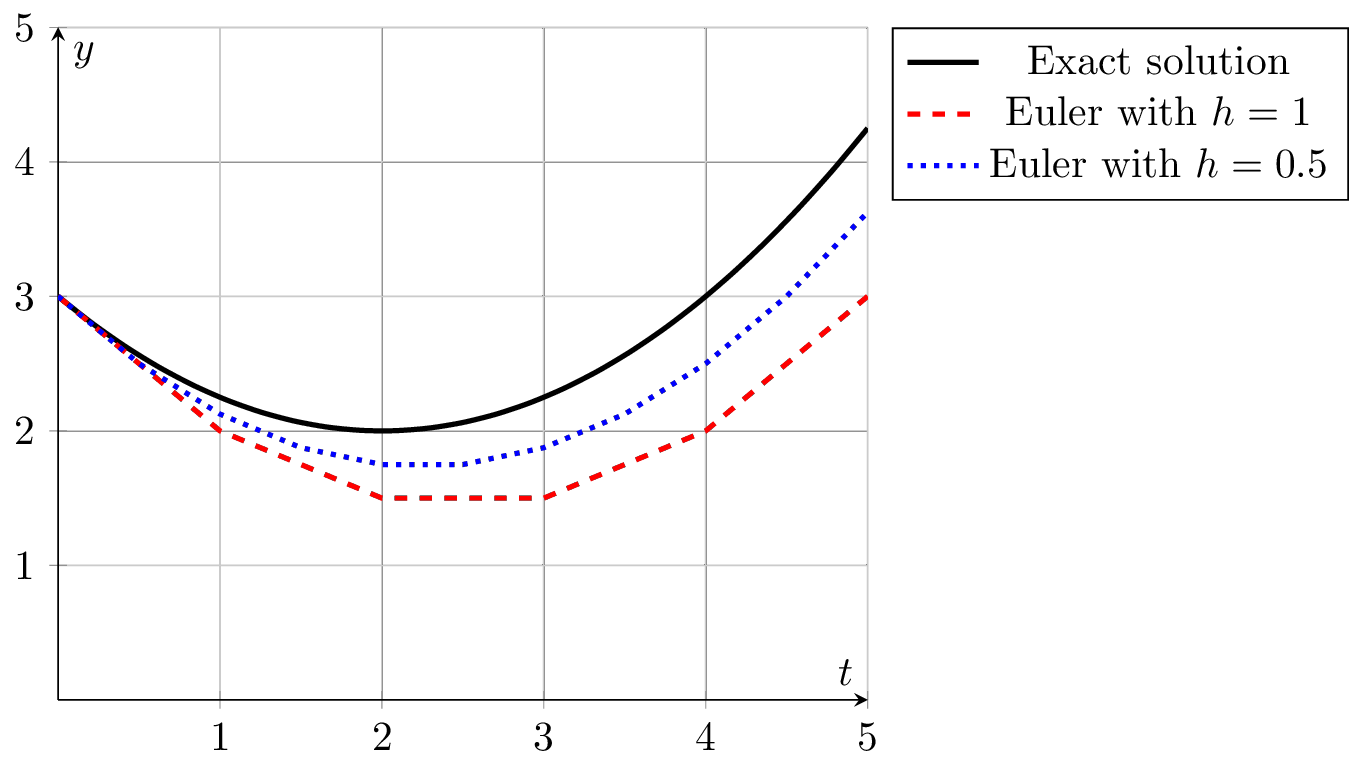
\includegraphics[width=0.7\linewidth]{images/Ch05_Euler} 

}

\caption{Numerical solutions to a differential equation using Euler's method.}\label{fig:Euler}
\end{figure}

\begin{center}\rule{0.5\linewidth}{0.5pt}\end{center}

\begin{exercise}
\protect\hypertarget{exr:unnamed-chunk-424}{}{\label{exr:unnamed-chunk-424} }Why would Euler's method overshoot the exact solution in regions where the solution exhibits high curvature?
\end{exercise}

\begin{center}\rule{0.5\linewidth}{0.5pt}\end{center}

\begin{exercise}
\protect\hypertarget{exr:unnamed-chunk-425}{}{\label{exr:unnamed-chunk-425} }Write code to implement Euler's method for initial value problems. Your
function should accept as input a Python function \(f(t,x)\), an initial condition, a start time, an end time, and the value of \(h = \Delta t\). The output should be vectors for \(t\) and \(x\) that you can easily plot to show the numerical solution. The code below will get you started.
\end{exercise}

\begin{Shaded}
\begin{Highlighting}[]
\KeywordTok{def}\NormalTok{ euler1d(f,x0,t0,tmax,dt):}
\NormalTok{    t }\OperatorTok{=} \CommentTok{\# set up the domain based on t0, tmax, and dt}
\NormalTok{    x }\OperatorTok{=}\NormalTok{ np.zeros\_like(t) }\CommentTok{\# set up a zeros vector for x that is the same size a t}
\NormalTok{    x[}\DecValTok{0}\NormalTok{] }\OperatorTok{=} \CommentTok{\# fill in the initial condition}
    \ControlFlowTok{for}\NormalTok{ n }\KeywordTok{in} \BuiltInTok{range}\NormalTok{( ??? ): }\CommentTok{\# carefully think about how far we should loop}
\NormalTok{        x[n}\OperatorTok{+}\DecValTok{1}\NormalTok{] }\OperatorTok{=} \CommentTok{\# use Euler\textquotesingle{}s method to advance the solution forward in time}
    \ControlFlowTok{return}\NormalTok{ t, x}
\end{Highlighting}
\end{Shaded}

\begin{center}\rule{0.5\linewidth}{0.5pt}\end{center}

\begin{exercise}
\protect\hypertarget{exr:unnamed-chunk-427}{}{\label{exr:unnamed-chunk-427} }Test your code from the previous exercise on a first order differential equation where you know the answer. Then test your code on the differential equation
\[x' = -\frac{1}{3}x+\sin(t) \quad \text{where} \quad x(0) = 1.\]
The partial code below should get you started.
\end{exercise}

\begin{Shaded}
\begin{Highlighting}[]
\ImportTok{import}\NormalTok{ numpy }\ImportTok{as}\NormalTok{ np}
\ImportTok{import}\NormalTok{ matplotlib.pyplot }\ImportTok{as}\NormalTok{ plt}
\CommentTok{\# put the f(t,x) function on the next line }
\CommentTok{\# (be sure to specify t even if it doesn\textquotesingle{}t show up in your test ODEs)}
\NormalTok{f }\OperatorTok{=} \KeywordTok{lambda}\NormalTok{ t, x: }\CommentTok{\# your function goes here}
\NormalTok{x0 }\OperatorTok{=} \CommentTok{\# initial condition}
\NormalTok{t0 }\OperatorTok{=} \CommentTok{\# initial time}
\NormalTok{tmax }\OperatorTok{=} \CommentTok{\# final time (your choice)}
\NormalTok{dt }\OperatorTok{=} \CommentTok{\# Delta t (your choice, but make it small)}
\NormalTok{t, x }\OperatorTok{=}\NormalTok{ euler1d(f,x0,t0,tmax,dt)}
\NormalTok{plt.plot(t,x,}\StringTok{\textquotesingle{}b{-}\textquotesingle{}}\NormalTok{)}
\NormalTok{plt.grid()}
\NormalTok{plt.show()}
\end{Highlighting}
\end{Shaded}

\begin{center}\rule{0.5\linewidth}{0.5pt}\end{center}

\begin{exercise}
\protect\hypertarget{exr:ode-error-analysis}{}{\label{exr:ode-error-analysis} }The differential equation
\(x' = -\frac{1}{3}x + \sin(t)\) with \(x(0) = 1\) has an analytic solution
\[x(t) = \frac{1}{10} \left( 19 e^{-t/3} + 3\sin(t) - 9\cos(t) \right).\]
The goal of this problem will be to compare the maximum error on the
interval \(t \in  [0,5]\) for various values of \(\Delta t\) in your Euler solver.

\begin{enumerate}
\def\labelenumi{\alph{enumi}.}
\item
  Write code that gives the maximum point-wise error between your
  numerical solution and the analytic solution given a value of
  \(\Delta t\).
\item
  Using your code from part (a), build a plot with the value of
  \(\Delta t\) on the horizontal axis and the value of the
  associated error on the vertical axis. You should use a log-log
  plot. Obviously you will need to run your code many times at many
  different values of \(\Delta t\) to build your data set.
\item
  In general, if you were to cut your value of \(\Delta t\) in half,
  what would that do to the value of the error? What about dividing
  \(\Delta t\) by 10? 100? 1000?
\end{enumerate}
\end{exercise}

\begin{center}\rule{0.5\linewidth}{0.5pt}\end{center}

\begin{exercise}
\protect\hypertarget{exr:unnamed-chunk-429}{}{\label{exr:unnamed-chunk-429} }Shelby solved a first order ODE \(x' = f(t,x)\) using Euler's method with a step size of \(dt = 0.1\) on a domain \(t \in [0,3]\). To test her code she used a differential equation where she new the exact analytic solution and she found the maximum absolute error on the interval to be \(0.15\). Jackson then solves the exact same differential equation, on the same interval, with the same initial condition using Euler's method and a step size of \(dt = 0.01\). What is Jackson's expected maximum absolute error?
\end{exercise}

\begin{center}\rule{0.5\linewidth}{0.5pt}\end{center}

\begin{theorem}
\protect\hypertarget{thm:unnamed-chunk-430}{}{\label{thm:unnamed-chunk-430} }Euler's method is a first order method for approximating the solution to the differential equation \(x' = f(t,x)\). Hence, if the step size \(h\) of the partition of the domain were to be divided by some positive constant \(M\) then the maximum absolute error between the numerical solution and the exact solution would ???\\
(Complete the last sentence.)
\end{theorem}

\begin{center}\rule{0.5\linewidth}{0.5pt}\end{center}

\begin{exercise}
\protect\hypertarget{exr:unnamed-chunk-431}{}{\label{exr:unnamed-chunk-431} }If we want to numerically solve the first order differential equation \(x' = f(t,x)\) on the interval \(t \in [0,1]\) with Euler's method so that we realize a maximum absolute error of \(10^{-8}\) between the numerical solution and the exact solution, then how many points do we need to subdivide the interval \([0,1]\) into?
\end{exercise}

\begin{center}\rule{0.5\linewidth}{0.5pt}\end{center}

\begin{exercise}
\protect\hypertarget{exr:euler-multi-dimensional}{}{\label{exr:euler-multi-dimensional} }If a mass is hanging from a spring then Newton's second law, \(\sum F=ma\), gives us the differential equation \(mx'' = F_{restoring} + F_{damping}\) where \(x\) is the displacement of the mass from equilibrium, \(m\) is the mass of the object hanging from the spring, \(F_{restoring}\) is the force pulling the mass back to equilibrium, and \(F_{damping}\) is the force due to friction or air resitance that slows the mass down.

\begin{enumerate}
\def\labelenumi{\alph{enumi}.}
\tightlist
\item
  Which of the following is a good candidate for a restoring force in a spring? Defend your answer.

  \begin{enumerate}
  \def\labelenumii{\roman{enumii}.}
  \tightlist
  \item
    \(F_{restoring} = kx\): The restoring force is proportional to the displacement away from equilibrium.
  \item
    \(F_{restoring} = kx'\): The restoring force is proportional to the velocity of the mass.
  \item
    \(F_{restoring} = kx''\): The restoring force is proportional to the acceleration of the mass.
  \end{enumerate}
\item
  Which of the following is a good candidate for a damping force in a spring? Defend your answer.

  \begin{enumerate}
  \def\labelenumii{\roman{enumii}.}
  \tightlist
  \item
    \(F_{restoring} = bx\): The damping force is proportional to the displacement away from equilibrium.
  \item
    \(F_{restoring} = bx'\): The damping force is proportional to the velocity of the mass.
  \item
    \(F_{restoring} = bx''\): The damping force is proportional to the acceleration of thte mass.
  \end{enumerate}
\item
  Put your answers to parts (a) and (b) together and simplify to form a second-order differential equation for position:
  \[ \underline{\hspace{0.25in}} x'' + \underline{\hspace{0.25in}} x' + \underline{\hspace{0.25in}} x = 0 \]
\item
  If we want to solve a second order differential equation numerically we need to convert it to first order differential equations (Euler's method is only designed to deal with first order differential equations, not second order). To do so we can introduce a new variable, \(x_1\), such that \(x_1 = x'\). For the sake of notational consistency we define \(x_0 = x\). The result is a system of first-order differential equations.
  \[\begin{aligned} x_0' &= x_1 \\ x_1' &= \underline{\hspace{2in}} \end{aligned}\]
\item
  The code and Euler's method algorithm that we've created thus far in this chapter are only designed to work with a single differential equation instead of a system, so we need to make some modifications. We can discretize the system of differential equations using Euler's method so that
  \[ \boldsymbol{x}' = F(t,\boldsymbol{x}) \]
  where \(F\) is a function that accepts a vector of inputs, plus time, and returns a vector of outputs. In the context of this particular problem,
  \[ F(t,\boldsymbol{x}) = \begin{pmatrix} x_0' \\ x_1' \end{pmatrix} = \begin{pmatrix} x_1 \\ \underline{\hspace{1in}} \end{pmatrix} \]
\item
  We now need to discretize the derivatives in the system. As with 1D Euler's method, we will use a first-order approximation of the first derivative so that
  \[ \frac{\boldsymbol{x}_{n+1} - \boldsymbol{x}_n }{h} = F(t_n,\boldsymbol{x}_n) + \mathcal{O}(h). \]
  Rearranging and solving for \(\boldsymbol{x}_{n+1}\) gives
  \[ \boldsymbol{x}_{n+1} = \underline{\hspace{0.5in}} + h F( \underline{\hspace{0.25in}} , \underline{\hspace{0.25in}}). \]
\item
  We now have a choice about how we're going to code this new 2D version of Euler's method. We could just include one more input function and one more input initial condition into the \texttt{euler()} function so that the Python function call is \texttt{euler(f0,f1,x0,x1,t0,tmax,dt)} where \texttt{f0} and \texttt{f1} are the two right-hand sides of the system, and \texttt{x0} and \texttt{x1} are the two initial conditions. Alternatively, we could rethink our \texttt{euler()} function so that it accepts an array of functions and an array of initial conditions so that the Python function call is \texttt{euler(F,X,t0,tmax,dt)} where \texttt{F} is a Python array of functions and \texttt{X} is a Python array of initial conditions. Discuss the pros and cons of each approach.\\
\item
  The following Python function and associated script will implement the vector version of Euler's method. Complete the code and then use it to solve the system of equations from part (d). Use a mass of \(m=2\)kg, a damping force of \(b=40\)kg/s, and a spring constant of \(k=128\)N/m. Consider an initial position of \(x=0\)m (equilibrium) and an initial velocity of \(x_1 = 0.6\)m/s. Show two plots: a plot that shows both position and velocity vs time and a second plot, called a phase plot, that shows position vs velocity.
\end{enumerate}
\end{exercise}

\begin{Shaded}
\begin{Highlighting}[]
\KeywordTok{def}\NormalTok{ euler(F,x0,t0,tmax,dt):}
\NormalTok{    t }\OperatorTok{=} \CommentTok{\# same code as before to set up a vector for time}
    \CommentTok{\# Next we set up x so that it is an array where the rows are the }
    \CommentTok{\# different dimensions of the problem.  For example, in this }
    \CommentTok{\# problem there will be 2 rows and len(t) columns.}
\NormalTok{    x }\OperatorTok{=}\NormalTok{ np.zeros( (}\BuiltInTok{len}\NormalTok{(x0), }\BuiltInTok{len}\NormalTok{(t)) ) }
\NormalTok{    x[:,}\DecValTok{0}\NormalTok{] }\OperatorTok{=}\NormalTok{ x0 }\CommentTok{\# store the initial condition in the first column}
    \ControlFlowTok{for}\NormalTok{ n }\KeywordTok{in} \BuiltInTok{range}\NormalTok{(}\BuiltInTok{len}\NormalTok{(t)}\OperatorTok{{-}}\DecValTok{1}\NormalTok{):}
\NormalTok{        x[:,n}\OperatorTok{+}\DecValTok{1}\NormalTok{] }\OperatorTok{=}\NormalTok{ x[ ??? , ??? ] }\OperatorTok{+}\NormalTok{ dt}\OperatorTok{*}\NormalTok{F(t[ ??? ], x[ ??? , ??? ])}
    \ControlFlowTok{return}\NormalTok{ t, x}
\end{Highlighting}
\end{Shaded}

To use the \texttt{euler()} function defined above we can use the following code. Fill in the code for this system of differential equations with this problem.

\begin{Shaded}
\begin{Highlighting}[]
\NormalTok{F }\OperatorTok{=} \KeywordTok{lambda}\NormalTok{ t, x: np.array([ x[}\DecValTok{1}\NormalTok{] , ??? ])}
\NormalTok{x0 }\OperatorTok{=}\NormalTok{ [ ??? , ??? ] }\CommentTok{\# initial conditions}
\NormalTok{t0 }\OperatorTok{=} \DecValTok{0}
\NormalTok{tmax }\OperatorTok{=} \DecValTok{5} \CommentTok{\# pick something reasonable here}
\NormalTok{dt }\OperatorTok{=} \FloatTok{0.01} \CommentTok{\# your choice.  pick something small}
\NormalTok{t, x }\OperatorTok{=}\NormalTok{ euler(F,x0,t0,tmax,dt)}
\CommentTok{\# Next we plot.  }
\NormalTok{plt.plot(t,x[ ??? ,:],}\StringTok{\textquotesingle{}b{-}\textquotesingle{}}\NormalTok{,t,x[ ??? ,:],}\StringTok{\textquotesingle{}r{-}{-}\textquotesingle{}}\NormalTok{)}
\NormalTok{plt.grid()}
\NormalTok{plt.title(}\StringTok{\textquotesingle{}Time Evolution of Position and Velocity\textquotesingle{}}\NormalTok{)}
\NormalTok{plt.legend([}\StringTok{\textquotesingle{}which legend entry here\textquotesingle{}}\NormalTok{,}\StringTok{\textquotesingle{}which legend entry here\textquotesingle{}}\NormalTok{])}
\NormalTok{plt.xlabel(}\StringTok{\textquotesingle{}time\textquotesingle{}}\NormalTok{)}
\NormalTok{plt.ylabe(}\StringTok{\textquotesingle{}position and velocity\textquotesingle{}}\NormalTok{)}
\NormalTok{plt.show()}

\NormalTok{plt.plot(x[???, :], x[???, :], }\StringTok{\textquotesingle{}k{-}{-}\textquotesingle{}}\NormalTok{)}
\NormalTok{plt.grid()}
\NormalTok{plt.title(}\StringTok{\textquotesingle{}Phase Plot\textquotesingle{}}\NormalTok{)}
\NormalTok{plt.xlabel(}\StringTok{\textquotesingle{}position\textquotesingle{}}\NormalTok{)}
\NormalTok{plt.ylabel(}\StringTok{\textquotesingle{}velocity\textquotesingle{}}\NormalTok{)}
\NormalTok{plt.show()}
\end{Highlighting}
\end{Shaded}

\begin{center}\rule{0.5\linewidth}{0.5pt}\end{center}

\begin{exercise}
\protect\hypertarget{exr:unnamed-chunk-434}{}{\label{exr:unnamed-chunk-434} }Consider a collection of two connected mass-spring oscillators where there is a mass hanging from a fixture and a second mass is connected directly to the first (hanging vertically). For simplicity in this problem we will neglect damping. Let \(k_1\) and \(k_2\) be the spring constants for the two springs, respectively.

\begin{enumerate}
\def\labelenumi{\alph{enumi}.}
\tightlist
\item
  Draw a picture of the physical setup described. Let \(x_1\) be the position of mass 1 relative to its equilibrium. Let \(x_2\) be the position of mass 2 relative to its equilibrium. Label the coordinate systems for the two springs on your picture.
\item
  Give a thorough explanation for why the following second order differential equation models the position of the first mass
  \[ m x_1'' = -k_1 x_1 - k_2 (x_1 - x_2).  \]
\item
  Using similar logic from part (b), write a second order differential equation for the position of the second mass
  \[ m x_2'' = \underline{\hspace{2in}} \]
\item
  We now have a system of two second order differential equations. We can convert this to four first order differential equations by introducing two new variables: \(x_3 = x_1'\) and \(x_4 = x_2'\). Write the full system of first order differential equations.
\item
  Use your vector-based \texttt{euler()} function to numerically solve the system of equations in several different physical scenarios. There are four variables so you will need to think carefully about which plots are the most explanatory. Also, if may be easiest to take \(k_1 = 1\) and then take \(k_2\) as the stiffness of spring 2 relative to spring 1 (e.g.~if \(k_2 = 1\) then the springs are the same stiffness, if \(k_2 = 0.5\) then spring 2 is half as still, etc).
\end{enumerate}
\end{exercise}

\begin{center}\rule{0.5\linewidth}{0.5pt}\end{center}

\begin{exercise}
\protect\hypertarget{exr:unnamed-chunk-435}{}{\label{exr:unnamed-chunk-435} }Extend the previous exercise to that there are three masses hanging in a chain.
\end{exercise}

\begin{center}\rule{0.5\linewidth}{0.5pt}\end{center}

\begin{exercise}
\protect\hypertarget{exr:unnamed-chunk-436}{}{\label{exr:unnamed-chunk-436} }If the speed of the mass in the mass-spring oscillator is \emph{fast enough} then the damping force will no longer just be proportional to the velocity. Instead, at higher speeds the drag force is proportional to the square of the velocity. You can think of this as a bungee jumper jumping off of a bridge. Modify the single mass-spring oscillator equation to allow for nonlinear quadratic damping. Solve the system numerically under several different physical conditions (stiff spring, non-stiff spring, high damping, low damping, different initial conditions, etc).
\end{exercise}

\begin{center}\rule{0.5\linewidth}{0.5pt}\end{center}

\begin{exercise}[A Lotka-Volterra Model]
\protect\hypertarget{exr:unnamed-chunk-437}{}{\label{exr:unnamed-chunk-437} \iffalse (A Lotka-Volterra Model) \fi{} }Test your code from the previous problems on the following system of differential equations by showing a time evolution plot (time on \(x_0\) and populations on \(x_1\)) as well as a phase plot (\(x_0\) on the \(x\) and \(x_1\) on the \(y\) with time understood implicitly):\\
\textbf{The Lotka-Volterra Predator-Prey Model:}\\
Let \(x_0(t)\) denote the number of rabbits (prey) and \(x_1(t)\) denote the
number of foxes (predator) at time \(t\). The relationship between the
species can be modeled by the classic 1920's Lotka-Volterra Model:
\[\left\{ \begin{array}{ll} x_0' &= \alpha x_0 - \beta x_0 x_1 \\ x_1' &= \delta x_0 x_1 - \gamma x_1 \end{array} \right.\]
where \(\alpha, \beta, \gamma,\) and
\(\delta\) are positive constants. For this problems take
\(\alpha \approx 1.1\), \(\beta \approx 0.4\), \(\gamma \approx 0.1\), and
\(\delta \approx 0.4\).

\begin{enumerate}
\def\labelenumi{\alph{enumi}.}
\tightlist
\item
  First rewrite the system of ODEs in the form \(\boldsymbol{x}' = F(t,\boldsymbol{x})\) so you can use your \texttt{euler()} code.\\
\item
  Modify your code from the previous problem so that it works for this problem. Use \texttt{tmax\ =\ 200} and an appropriately small time step.
\item
  Create the time evolution plot. What does this plot tell you in context?
\item
  Create a phase plot. What does this plot tell you in context?\\
\item
  If you cut your time step in half, what do you see in the two plots? Why? What is Euler's method doing here?
\end{enumerate}
\end{exercise}

\begin{center}\rule{0.5\linewidth}{0.5pt}\end{center}

\begin{exercise}[The SIR Model]
\protect\hypertarget{exr:unnamed-chunk-438}{}{\label{exr:unnamed-chunk-438} \iffalse (The SIR Model) \fi{} }A classic model for predicting the spread of a virus or a disease is the SIR Model. In these models, \(S\) stands for the proportion of the population which is susceptible to the virus, \(I\) is the proportion of the population that is currently infected with the virus, and \(R\) is the proportion of the population that has recovered from the virus. The idea behind the model is that

\begin{itemize}
\tightlist
\item
  Susceptible people become infected by hanving interaction with the infected people. Hence, the rate of change of the susceptible people is proportional to the number of interactions that can occur between the \(S\) and the \(I\) populations.\\
  \[ S' = -\alpha SI \]
\item
  The infected population gains people from the interactions with the susceptible people, but at the same time, infected people recover at a predictable rate.
  \[ I' = \alpha SI - \beta I \]
\item
  The people in the recovered class are then immune to the virus, so the recovered class \(R\) only gains people from the recoveries from the \(I\) class.
  \[ R' = \beta I \]
\end{itemize}

\begin{enumerate}
\def\labelenumi{\alph{enumi}.}
\tightlist
\item
  Explain the minus sign in the \(S'\) equation in the context of the spread of a virus.
\item
  Explain the product \(SI\) in the \(S'\) equation in the context of the spread of a virus.
\item
  Find a numerical solution to the system of equations using your \texttt{euler()} function. Use the parameters \(\alpha = 0.4\) and \(\beta = 0.04\) with initial conditions \(S(0) = 0.99\), \(I(0) = 0.01\), and \(R(0) = 0\). Explain all three curves in context.
\end{enumerate}
\end{exercise}

\begin{center}\rule{0.5\linewidth}{0.5pt}\end{center}

\hypertarget{the-midpoint-method}{%
\section{The Midpoint Method}\label{the-midpoint-method}}

Now we get to improve upon Euler's method. There is a long history of wonderful improvements to the classic Euler's method -- some that work in special cases, some that resolve areas where the error is going to be high, and some that are great for general purpose numerical solutions to ODEs with relatively high accuracy. In this section we'll make a simple modification to Euler's method that has a surprisingly great payoff in the error rate.

\begin{center}\rule{0.5\linewidth}{0.5pt}\end{center}

\begin{exercise}
\protect\hypertarget{exr:unnamed-chunk-439}{}{\label{exr:unnamed-chunk-439} }In Euler's method, if we are at the point \(t_n\) then we approximate the slope \(x'(t_n) = f(t_n,x_n)\) and use the slope to propagate forward one time step. As you have seen, this method can lead to an overshooting of the exact solution in regions of high curvature. It would be nice to be able to look into the future and get a better approximation of the slope so that we didn't miss upcoming curvature. If you could build such a method that looks in to the future, finds a slope in the future, and then uses that slope (instead of the slope from Euler's method) to advance forward in time, how far into the future would you look? Why?
\end{exercise}

\begin{center}\rule{0.5\linewidth}{0.5pt}\end{center}

\begin{exercise}
\protect\hypertarget{exr:unnamed-chunk-440}{}{\label{exr:unnamed-chunk-440} }Let's return to the simple differential equation \(x' = -0.5x\) with
\(x(0) = 6\) that we saw in Exercise \ref{exr:euler-motivation}. Now we'll propose a slightly different method for approximating the solution.

\begin{enumerate}
\def\labelenumi{\alph{enumi}.}
\tightlist
\item
  At \(t=0\) we know that \(x(0)=6\). If we use the slope at time \(t=0\) to step forward in time then we will get the Euler approximation of the solution. Consider this alternative approach:
\end{enumerate}

\begin{itemize}
\tightlist
\item
  Use the slope at time \(t=0\) and move \emph{half} a step forward.
\item
  Find the slope at the half-way point
\item
  Then use the slope from the half way point to go a full step forward from time \(t=0\).
\end{itemize}

Perhaps a bit confusing \ldots let's build this idea together:

\begin{itemize}
\tightlist
\item
  What is the slope at time \(t=0\)? \(x'(0) = \underline{\hspace{0.5in}}\)
\item
  Use this slope to step a half step forward and find the \(x\) value: \(x(0.5) \approx \underline{\hspace{0.5in}}\)
\item
  Now use the differential equation to find the slope at time \(t=0.5\). \(x(0.5) = \underline{\hspace{0.5in}}\)
\item
  Now take your answer from the previous step, and go one full step forward from time \(t=0\). What \(x\) value do you end up with?
\item
  Your answers to the previous bullets should be: \(x'(0) = -3\), \(x(0.5) \approx 4.5\), \(x'(0.5) = -2.25\), so if we take a full step forward with slope \(m=-2.25\) starting from \(t=0\) we get \(x(1) \approx 3.75\).
\end{itemize}

\begin{enumerate}
\def\labelenumi{\alph{enumi}.}
\setcounter{enumi}{1}
\tightlist
\item
  Repeat the process outlined in part (a) to approximate the solution to the differential equation at times \(t=2, 3, \ldots, 10\). Also record the exact answer at each of these times.
\end{enumerate}

\begin{longtable}[]{@{}llllllllllll@{}}
\toprule
\(t\) & 0 & 1 & 2 & 3 & 4 & 5 & 6 & 7 & 8 & 9 & 10\tabularnewline
\midrule
\endhead
Approximation of \(x(t)\) & 6 & & & & & & & & & &\tabularnewline
Exact value of \(x(t)\) & 6 & & & & & & & & & &\tabularnewline
\bottomrule
\end{longtable}

\begin{enumerate}
\def\labelenumi{\alph{enumi}.}
\setcounter{enumi}{2}
\item
  Draw a clear picture of what this method is doing in order to approximate the slope at each individual step.
\item
  How does your approximation compare to the Euler approximation that you found in Exercise \ref{exr:euler-motivation}?
\end{enumerate}
\end{exercise}

\begin{center}\rule{0.5\linewidth}{0.5pt}\end{center}

\begin{definition}[The Midpoint Method]
\protect\hypertarget{def:midpoint}{}{\label{def:midpoint} \iffalse (The Midpoint Method) \fi{} }The midpoint method is defined by first taking a half step with Euler's method to approximate a solution at time \(t_{n+1/2}\) There is not grid point at \(t_{n+1/2}\) so we define this as \$ t\_\{n+1/2\} = (t\_n + t\_\{n+1\})/2\$. We then take a full step using the value of \(f\) at \(t_{n+1/2}\) and the approximate \(x_{n+1/2}\).
\[\begin{aligned}
        x_{n+1/2} &= x_n + \frac{h}{2} f(t_n,x_n) \\
        x_{n+1} &= x_n + h f(t_{n+1/2},x_{n+1/2})
    \end{aligned}\]
Note: Indexing by \(1/2\) in a computer is nonsense. Instead, we implement the midpoint method with: \[\begin{aligned}
        m_n &= f(t_n,x_n) \\
        x_{temp} &= x_n + \frac{h}{2} m_n \\
        x_{n+1} &= x_n + h f\left( t_n + \frac{\Delta t}{2}, x_{temp}\right)
    \end{aligned}\]
\end{definition}

\begin{center}\rule{0.5\linewidth}{0.5pt}\end{center}

\begin{exercise}
\protect\hypertarget{exr:unnamed-chunk-441}{}{\label{exr:unnamed-chunk-441} }Complete the code below to implement the midpoint method in one dimension.
\end{exercise}

\begin{Shaded}
\begin{Highlighting}[]
\KeywordTok{def}\NormalTok{ midpoint1d(f,x0,t0,tmax,dt):}
\NormalTok{    t }\OperatorTok{=} \CommentTok{\# build the times}
\NormalTok{    x }\OperatorTok{=} \CommentTok{\# build an array for the x values}
\NormalTok{    x[}\DecValTok{0}\NormalTok{] }\OperatorTok{=} \CommentTok{\# build the initial condition}
    \ControlFlowTok{for}\NormalTok{ n }\KeywordTok{in} \BuiltInTok{range}\NormalTok{( ??? ): }\CommentTok{\# be careful about how far you\textquotesingle{}re looping}
        \CommentTok{\# The interesting part of the code goes here.}
    \ControlFlowTok{return}\NormalTok{ t, x}
\end{Highlighting}
\end{Shaded}

Test your code on several differential equations where you know the solution (just to be sure that it is working).

\begin{Shaded}
\begin{Highlighting}[]
\NormalTok{f }\OperatorTok{=} \KeywordTok{lambda}\NormalTok{ t, x: }\CommentTok{\# your ODE right hand side goes here}
\NormalTok{x0 }\OperatorTok{=} \CommentTok{\# initial condition}
\NormalTok{t0 }\OperatorTok{=} \DecValTok{0}
\NormalTok{tmax }\OperatorTok{=} \CommentTok{\# ending time (up to you)}
\NormalTok{dt }\OperatorTok{=} \CommentTok{\# pick something small}
\NormalTok{t, x }\OperatorTok{=}\NormalTok{ midpoint1d( ??? , ??? , ??? , ??? , ??? )}
\NormalTok{plt.plot( ??? , ??? , ??? )}
\NormalTok{plt.grid()}
\NormalTok{plt.show()}
\end{Highlighting}
\end{Shaded}

\begin{center}\rule{0.5\linewidth}{0.5pt}\end{center}

\begin{exercise}
\protect\hypertarget{exr:unnamed-chunk-444}{}{\label{exr:unnamed-chunk-444} }The goal in building the midpoint method was to hopefully capture some of the upcoming curvature in the solution before we overshot it. Consider the differential equation \(x' = -0.25x + \sin(t)\) with initial condition \(x(0) = 1\) on the domain \(t \in [0,4]\). First get a numerical solution with Euler's method using \(\Delta t = 0.1\). Then get a numerical solution with the midpoint method using the same value for \(\Delta t\). Plot the two solutions on top of each other along with the exact solution
\[ x(t) = \frac{1}{10} \left( 19e^{-t/3} + 3\sin(t) - 9\cos(t)  \right). \]
What do you observe? What do you observe if you make \(\Delta t\) a bit larger (like 0.2 or 0.3)? What do you observe if you make \(\Delta t\) very very small (like 0.001 or 0.0001)?

There are several key takeaways from this problem. Discuss.
\end{exercise}

\begin{center}\rule{0.5\linewidth}{0.5pt}\end{center}

\begin{exercise}
\protect\hypertarget{exr:unnamed-chunk-445}{}{\label{exr:unnamed-chunk-445} }Repeat Exercise \ref{exr:ode-error-analysis} with the midpoint method. Compare your results to what you found with Euler's method.
\end{exercise}

\begin{center}\rule{0.5\linewidth}{0.5pt}\end{center}

\begin{exercise}
\protect\hypertarget{exr:unnamed-chunk-446}{}{\label{exr:unnamed-chunk-446} }We have studied two methods thus far: Euler's method and the Midpoint method. In Figure \ref{fig:Euler-Midpoint} we see a graphical depiction of how each method works on the differential equation \(y' = y\) with \(\Delta t = 1\) and \(y(0) = 1\). The exact solution at \(t=1\) is \(y(1) = e^1 \approx 2.718\) and is shown in red in each figure. The methods can be summarized in the table below.

Discuss what you observe as the pros and cons of each method based on the table and on the Figure.
\end{exercise}

\begin{longtable}[]{@{}ll@{}}
\toprule
\begin{minipage}[b]{0.45\columnwidth}\raggedright
Euler's Method\strut
\end{minipage} & \begin{minipage}[b]{0.49\columnwidth}\raggedright
Midpoint Method\strut
\end{minipage}\tabularnewline
\midrule
\endhead
\begin{minipage}[t]{0.45\columnwidth}\raggedright
1. Get the slope at time \(t_n\)\strut
\end{minipage} & \begin{minipage}[t]{0.49\columnwidth}\raggedright
1. Get the slope at time \(t_n\)\strut
\end{minipage}\tabularnewline
\begin{minipage}[t]{0.45\columnwidth}\raggedright
2. Follow the slope for time \(\Delta t\)\strut
\end{minipage} & \begin{minipage}[t]{0.49\columnwidth}\raggedright
2. Follow the slope for time \(\Delta t/2\)\strut
\end{minipage}\tabularnewline
\begin{minipage}[t]{0.45\columnwidth}\raggedright
\strut
\end{minipage} & \begin{minipage}[t]{0.49\columnwidth}\raggedright
3. Get the slope at the point \(t_n + \Delta t/2\)\strut
\end{minipage}\tabularnewline
\begin{minipage}[t]{0.45\columnwidth}\raggedright
\strut
\end{minipage} & \begin{minipage}[t]{0.49\columnwidth}\raggedright
4. Follow the new slope from time \(t_n\) for time \(\Delta t\)\strut
\end{minipage}\tabularnewline
\bottomrule
\end{longtable}

\begin{figure}

{\centering 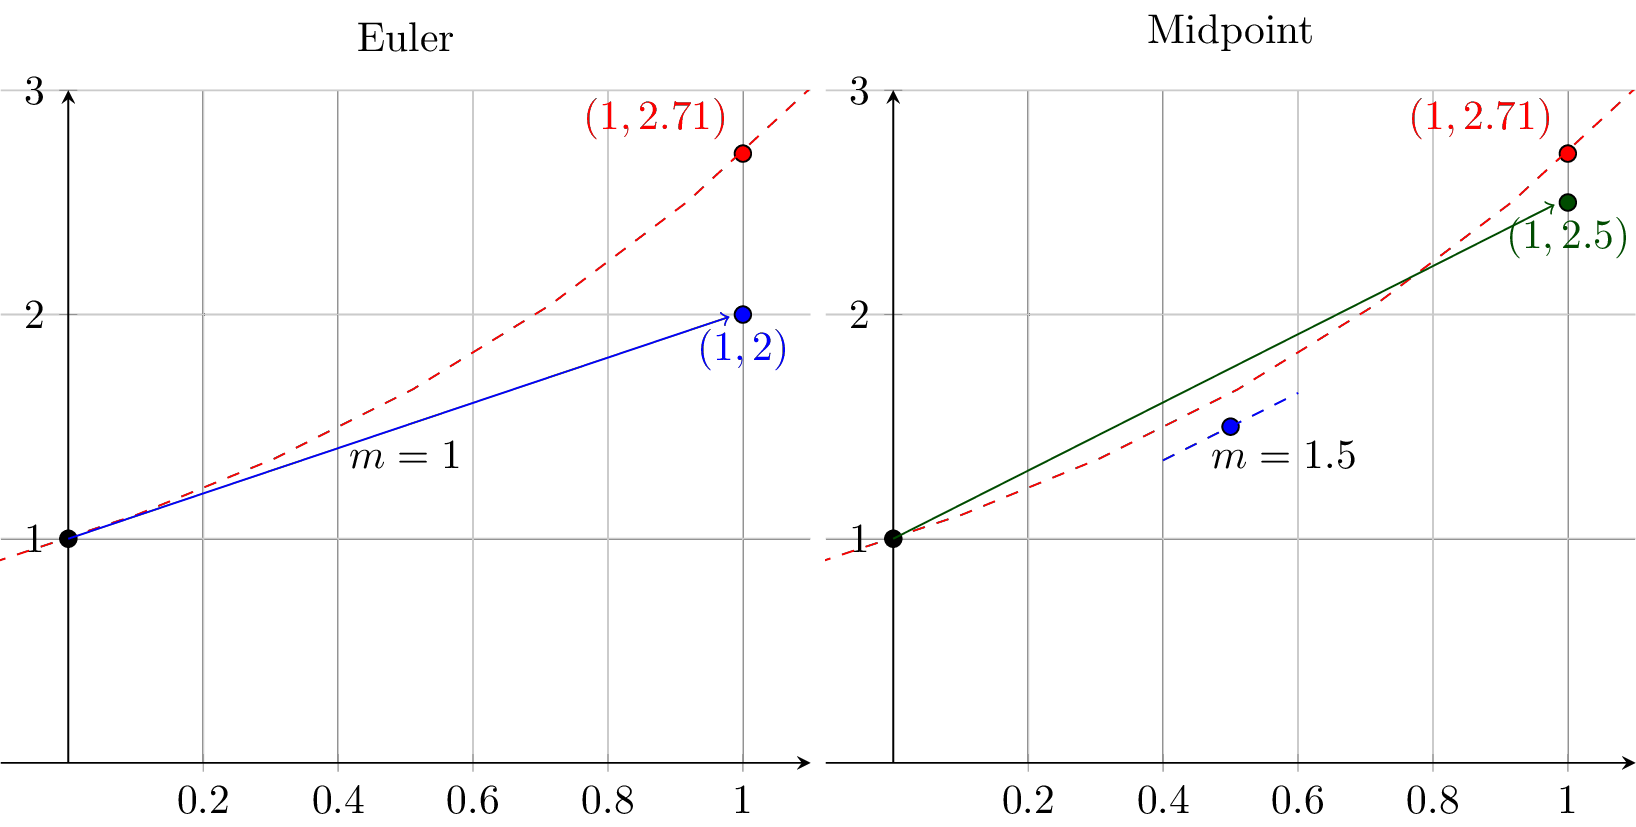
\includegraphics[width=0.9\linewidth]{images/Ch05_Midpoint} 

}

\caption{Graphical depictions of two numerical methods: Euler (left) and Midpoint (right). The exact solution is shown in red.}\label{fig:Euler-Midpoint}
\end{figure}

\begin{center}\rule{0.5\linewidth}{0.5pt}\end{center}

\begin{exercise}
\protect\hypertarget{exr:unnamed-chunk-447}{}{\label{exr:unnamed-chunk-447} }When might you want to use Euler's method instead of the midpoint
method? When might you want to use the midpoint method instead of
Euler's method?
\end{exercise}

\begin{center}\rule{0.5\linewidth}{0.5pt}\end{center}

\begin{exercise}[Midpoint Method in Several Dimensions]
\protect\hypertarget{exr:unnamed-chunk-448}{}{\label{exr:unnamed-chunk-448} \iffalse (Midpoint Method in Several Dimensions) \fi{} }Modify your \texttt{euler()} code from Exercise \ref{exr:euler-multi-dimensional} so that you can use the midoint method in as many dimensions as you like. You should only have to add one line of code and then be careful about the size of the arrays that are in play. Test your code on several problems. Compare and contract what you see with your Euler solutions and with your Midpoint solutions.
\end{exercise}

\begin{center}\rule{0.5\linewidth}{0.5pt}\end{center}

\hypertarget{the-runge-kutta-4-method}{%
\section{The Runge-Kutta 4 Method}\label{the-runge-kutta-4-method}}

OK. Ready for some experimentation? We are going to build a few experiments that eventually lead us to a very powerful method for finding numerical solutions to first order differential equations.

\begin{exercise}
\protect\hypertarget{exr:unnamed-chunk-449}{}{\label{exr:unnamed-chunk-449} }Let's talk about the Midpoint Method for a moment. The geometric idea of the midpoint method is outlined in the bullets below. Draw a picture along with the bullets.

\begin{itemize}
\tightlist
\item
  You're sitting at the point \((t_n,x_n)\).
\item
  The slope of the solution curve to the ODE where you're standing is
  \[ \text{slope at the point $(t_n,x_n)$ is: } m_n = f(t_n,x_n) \]
\item
  You take a half a step forward using the slope where you're standing. The new point, denoted \(x_{n+1/2}\), is given by
  \[ \text{location a half step forward is: } x_{n+1/2} = x_n + \frac{\Delta t}{2} m_n. \]
\item
  Now you're standing at \((t_n + \frac{\Delta t}{2} , x_{n+1/2})\) so there is a new slope here given by
  \[ \text{slope after a half of an Euler step is: } m_{n+1/2} = f(t_n+\Delta t/2,x_{n+1/2}). \]
\item
  Go back to the point \((t_n,x_n)\) and step a full step forward using slope \(m_{n+1/2}\). Hence the new approximation is
  \[ x_{n+1} = x_n + \Delta t \cdot m_{n+1/2} \]
\end{itemize}
\end{exercise}

\begin{center}\rule{0.5\linewidth}{0.5pt}\end{center}

\begin{exercise}
\protect\hypertarget{exr:unnamed-chunk-450}{}{\label{exr:unnamed-chunk-450} }One of the troubles with the midpoint method is that it doesn't actually use the information at the point \((t_n,x_n)\). Moreover, it doesn't leverage a slope at the next time step \(t_{n+1}\). Let's see what happens when we try a solution technique that combined the ideas of Euler and Midpoint as follows:

\begin{itemize}
\tightlist
\item
  The slope at the point \((t_n,x_n)\) can be called \(m_n\) and we find it by evaluating \(f(t_n,x_n)\).
\item
  The slope at the point \((t_{n+1/2}, x_{n+1/2})\) can be called \(m_{n+1/2}\) and we find it by evaluating \(f(t_{n+1/2}, x_{n+1/2})\).
\item
  We can now take a full step using slope \(m_{n+1/2}\) to get the point \(x_{n+1}\) and the slope there is \(m_{n+1} = f(t_{n+1}, x_{n+1})\).
\item
  Now we have three estimates of the slope that we can use to actually propagate forward from \((t_n,x_n)\):

  \begin{itemize}
  \tightlist
  \item
    We could just use \(m_n\). This is Euler's method.
  \item
    We could just use \(m_{n+1/2}\). This is the midpoint method.
  \item
    We could use \(m_{n+1}\). Would this approach be any good?
  \item
    We could use the average of the three slopes.
  \item
    We could use a weighted average of the three slopes where some preference is given to some slopes over the others.
  \end{itemize}
\end{itemize}

In the code below you will find a function called \texttt{ode\_test()} that you can use as a starting point to test our the last three ideas. After the function you will see several lines of code that test your method against the differential equation \(x'(t) = -\frac{1}{3}x + \sin(t)\) with \(x(0) = 1\). The plots that come out are our typical error plots with the step size on the horizontal axis and our maximum absolute error between the numerical solution and the exact solution on the vertical axis. Recall that the exact solution to this differential equation is
\[ x(t) = \frac{1}{10} \left( 19 e^{-t/3} + 3\sin(t) - 9\cos(t) \right) \]
\end{exercise}

\begin{Shaded}
\begin{Highlighting}[]
\ImportTok{import}\NormalTok{ numpy }\ImportTok{as}\NormalTok{ np}
\ImportTok{import}\NormalTok{ matplotlib.pyplot }\ImportTok{as}\NormalTok{ plt}

\CommentTok{\# *********}
\CommentTok{\# You should copy your euler and midpoint functions here. }
\CommentTok{\# We will be comparing to these two existing methods.}
\CommentTok{\# *********}

\KeywordTok{def}\NormalTok{ ode\_test(f,x0,t0,tmax,dt):}
\NormalTok{    t }\OperatorTok{=}\NormalTok{ np.arange(t0,tmax}\OperatorTok{+}\NormalTok{dt,dt) }\CommentTok{\# set up the times}
\NormalTok{    x }\OperatorTok{=}\NormalTok{ np.zeros(}\BuiltInTok{len}\NormalTok{(t)) }\CommentTok{\# set up the x}
\NormalTok{    x[}\DecValTok{0}\NormalTok{] }\OperatorTok{=}\NormalTok{ x0 }\CommentTok{\# initial condition}
    \ControlFlowTok{for}\NormalTok{ n }\KeywordTok{in} \BuiltInTok{range}\NormalTok{(}\BuiltInTok{len}\NormalTok{(t)}\OperatorTok{{-}}\DecValTok{1}\NormalTok{):}
\NormalTok{        m\_n }\OperatorTok{=}\NormalTok{ f(t[n],x[n])}
\NormalTok{        x\_n\_plus\_half }\OperatorTok{=}\NormalTok{ x[n] }\OperatorTok{+}\NormalTok{ (dt}\OperatorTok{/}\DecValTok{2}\NormalTok{)}\OperatorTok{*}\NormalTok{m\_n}
\NormalTok{        m\_n\_plus\_half }\OperatorTok{=}\NormalTok{ f( t[n]}\OperatorTok{+}\NormalTok{dt}\OperatorTok{/}\DecValTok{2}\NormalTok{ , x\_n\_plus\_half )}
\NormalTok{        x\_n }\OperatorTok{=}\NormalTok{ x[n] }\OperatorTok{+}\NormalTok{ dt }\OperatorTok{*}\NormalTok{ m\_n\_plus\_half}
\NormalTok{        m\_n\_plus\_1 }\OperatorTok{=}\NormalTok{ f(t[n]}\OperatorTok{+}\NormalTok{dt, x\_n )}
\NormalTok{        estimate\_of\_slope }\OperatorTok{=} \CommentTok{\# This is where you get to play}
\NormalTok{        x[n}\OperatorTok{+}\DecValTok{1}\NormalTok{] }\OperatorTok{=}\NormalTok{ x[n] }\OperatorTok{+}\NormalTok{ dt }\OperatorTok{*}\NormalTok{ estimate\_of\_slope}
    \ControlFlowTok{return}\NormalTok{ t, x}


\NormalTok{f }\OperatorTok{=} \KeywordTok{lambda}\NormalTok{ t, x: }\OperatorTok{{-}}\NormalTok{(}\DecValTok{1}\OperatorTok{/}\FloatTok{3.0}\NormalTok{)}\OperatorTok{*}\NormalTok{x }\OperatorTok{+}\NormalTok{ np.sin(t)}
\NormalTok{exact }\OperatorTok{=} \KeywordTok{lambda}\NormalTok{ t: (}\DecValTok{1}\OperatorTok{/}\FloatTok{10.0}\NormalTok{)}\OperatorTok{*}\NormalTok{(}\DecValTok{19}\OperatorTok{*}\NormalTok{np.exp(}\OperatorTok{{-}}\NormalTok{t}\OperatorTok{/}\DecValTok{3}\NormalTok{) }\OperatorTok{+} \DecValTok{3}\OperatorTok{*}\NormalTok{np.sin(t)}\OperatorTok{{-}}\DecValTok{9}\OperatorTok{*}\NormalTok{np.cos(t))}

\NormalTok{x0 }\OperatorTok{=} \DecValTok{1} \CommentTok{\# initial condition}
\NormalTok{t0 }\OperatorTok{=} \DecValTok{0} \CommentTok{\# initial time}
\NormalTok{tmax }\OperatorTok{=} \DecValTok{3} \CommentTok{\# max time}
\CommentTok{\# set up blank arrays to keep track of the maximum absolute errorrs}
\NormalTok{err\_euler }\OperatorTok{=}\NormalTok{ [] }
\NormalTok{err\_midpoint }\OperatorTok{=}\NormalTok{ []}
\NormalTok{err\_ode\_test }\OperatorTok{=}\NormalTok{ []}
\NormalTok{H }\OperatorTok{=} \FloatTok{10.0}\OperatorTok{**}\NormalTok{(}\OperatorTok{{-}}\NormalTok{np.arange(}\DecValTok{1}\NormalTok{,}\DecValTok{7}\NormalTok{,}\DecValTok{1}\NormalTok{)) }\CommentTok{\# give a list of Delta t values (what list did we give here)}
\ControlFlowTok{for}\NormalTok{ dt }\KeywordTok{in}\NormalTok{ H:}
\NormalTok{    t, xeuler }\OperatorTok{=}\NormalTok{ euler(f,x0,t0,tmax,dt) }\CommentTok{\# build an euler approximation}
\NormalTok{    err\_euler.append( np.}\BuiltInTok{max}\NormalTok{( np.}\BuiltInTok{abs}\NormalTok{( xeuler }\OperatorTok{{-}}\NormalTok{ exact(t) ) ) ) }\CommentTok{\# measure the max abs error}
\NormalTok{    t, xmidpoint }\OperatorTok{=}\NormalTok{ midpoint(f,x0,t0,tmax,dt) }\CommentTok{\# build a midpoint approximation}
\NormalTok{    err\_midpoint.append( np.}\BuiltInTok{max}\NormalTok{( np.}\BuiltInTok{abs}\NormalTok{( xmidpoint }\OperatorTok{{-}}\NormalTok{ exact(t) ) ) ) }\CommentTok{\# measure the max abs error}
\NormalTok{    t, xtest }\OperatorTok{=}\NormalTok{ ode\_test(f,x0,t0,tmax,dt) }\CommentTok{\# build your new approximation}
\NormalTok{    err\_ode\_test.append( np.}\BuiltInTok{max}\NormalTok{( np.}\BuiltInTok{abs}\NormalTok{( xtest }\OperatorTok{{-}}\NormalTok{ exact(t) ) ) ) }\CommentTok{\# measure the max abs error}

\CommentTok{\# Finally, we make a loglog plot of the errors.  }
\CommentTok{\# Keep an eye on the slopes since they tell you the order of the error for the method.}
\NormalTok{plt.loglog(H,err\_euler,}\StringTok{\textquotesingle{}r*{-}\textquotesingle{}}\NormalTok{,H,err\_midpoint,}\StringTok{\textquotesingle{}b*{-}\textquotesingle{}}\NormalTok{,H,err\_ode\_test,}\StringTok{\textquotesingle{}k*{-}\textquotesingle{}}\NormalTok{)}
\NormalTok{plt.grid()}
\NormalTok{plt.legend([}\StringTok{\textquotesingle{}euler\textquotesingle{}}\NormalTok{,}\StringTok{\textquotesingle{}midpoint\textquotesingle{}}\NormalTok{,}\StringTok{\textquotesingle{}test method\textquotesingle{}}\NormalTok{])}
\NormalTok{plt.show()}
\end{Highlighting}
\end{Shaded}

\begin{center}\rule{0.5\linewidth}{0.5pt}\end{center}

\begin{exercise}
\protect\hypertarget{exr:unnamed-chunk-452}{}{\label{exr:unnamed-chunk-452} }In the previous exercise you should have found that an average of the three slopes did just a \emph{little bit} better than the midpoint method but the order of the error (the slope in the loglog plot) stayed about the same. You should have also found that the weighted average
\[ \text{estimate of slope} = \frac{m_n + 2m_{n+1/2} + m_{n+1}}{4} \]
did just a little bit better than just an plain average. Why might this be? (If you haven't tried this weighted average then go back and try it.) Do other weighted averages of this sort work better or worse? Does it appear that we can improve upon the order of the error (the slope in the loglog plot) using any of these methods?
\end{exercise}

\begin{center}\rule{0.5\linewidth}{0.5pt}\end{center}

\begin{exercise}
\protect\hypertarget{exr:unnamed-chunk-453}{}{\label{exr:unnamed-chunk-453} }OK. Let's make one more modification. What if we built a fourth slope that resulted from stepping a half step forward using \(m_{n+1/2}\)? We'll call this \(m_{n+1/2}^*\) since it is a new estimate of \(m_{n+1/2}\).
\[ x_{n+1/2}^* = x_n + \frac{\Delta t}{2} m_{n+1/2} \]
\[ m_{n+1/2}^* = f(t_n + \Delta t/2, x_{n+1/2}^*) \]
Then calculate \(m_{n+1}\) using this new slope instead of what we did in the previous problem.

\begin{enumerate}
\def\labelenumi{\alph{enumi}.}
\tightlist
\item
  Draw a picture showing where this slope was calculated.
\item
  Modify the code from above to include this fourth slope.\\
\item
  Experiment with several ideas about how to best combine the four slopes: \(m_n, \, m_{n+1/2}, \, m_{n+1/2}^*,\) and \(m_{n+1}\).

  \begin{itemize}
  \tightlist
  \item
    Should we just take an average of the four slopes?
  \item
    Should we give one or more of the slopes preferential treatment and do some sort of weighted average?
  \item
    Should we do something else entirely?
  \end{itemize}
\end{enumerate}

Remember that we are looking to improve the slope in the loglog plot since that indicates an improvement in the order of the error (the accuracy) of the method.
\end{exercise}

\begin{center}\rule{0.5\linewidth}{0.5pt}\end{center}

\begin{exercise}
\protect\hypertarget{exr:unnamed-chunk-454}{}{\label{exr:unnamed-chunk-454} }In the previous exercise you no doubt experimented with many different linear combinations of \(m_n\), \(m_{n+1/2}\), \(m_{n+1/2}^*\), and \(m_n\). Many of the resulting numerical ODE methods likely had the same order of accuracy (again, the order of the method is the slope in the error plot), but some may have been much better or much worse. Work with your team to fill in the following summary table of all of the methods that you devised. If you generated linear combinations that are not listed below then just add them to the list (we've only listed the most common ones here).

\begin{longtable}[]{@{}lllllll@{}}
\toprule
Experiment Number & \(m_n\) & \(m_{n+1/2}\) & \(m_{n+1/2}^*\) & \(m_n\) & Order of Error & Name\tabularnewline
\midrule
\endhead
1 & 1 & 0 & 0 & 0 & \(\mathcal{O}(\Delta t)\) & Euler's Method\tabularnewline
2 & 0 & 1 & 0 & 0 & \(\mathcal{O}(\Delta t^2)\) & Midpoint Method\tabularnewline
3 & 1/2 & 1/2 & 0 & 0 & &\tabularnewline
4 & 1/3 & 1/3 & 0 & 1/3 & &\tabularnewline
5 & 1/4 & 2/4 & 0 & 1/4 & &\tabularnewline
6 & 0 & 0 & 1 & 0 & &\tabularnewline
7 & 0 & 1/2 & 1/2 & 0 & &\tabularnewline
8 & 1/3 & 1/3 & 1/3 & 0 & &\tabularnewline
9 & 1/4 & 1/4 & 1/4 & 1/4 & &\tabularnewline
10 & 1/5 & 2/5 & 1/5 & 1/5 & &\tabularnewline
11 & 1/5 & 1/5 & 2/5 & 1/5 & &\tabularnewline
11 & 1/6 & 2/6 & 2/6 & 1/6 & &\tabularnewline
12 & 1/6 & 3/6 & 1/6 & 1/6 & &\tabularnewline
13 & 1/6 & 1/6 & 3/6 & 1/6 & &\tabularnewline
14 & 1/7 & 2/7 & 3/7 & 1/7 & &\tabularnewline
15 & 1/8 & 3/8 & 3/8 & 1/8 & &\tabularnewline
16 & & & & & &\tabularnewline
17 & & & & & &\tabularnewline
\bottomrule
\end{longtable}
\end{exercise}

\begin{center}\rule{0.5\linewidth}{0.5pt}\end{center}

\begin{exercise}
\protect\hypertarget{exr:unnamed-chunk-455}{}{\label{exr:unnamed-chunk-455} }In the previous exercise you should have found at least one of the many methods to be far superior to the others. State which linear combination of slopes seems to have done the trick, draw a picture of what this method does to numerically approximate the next slope for a numerical solution to an ODE, and clearly state what the order of the error means about this method.
\end{exercise}

\begin{center}\rule{0.5\linewidth}{0.5pt}\end{center}

\begin{theorem}[The Runge-Kutta 4 Method]
\protect\hypertarget{thm:rk4}{}{\label{thm:rk4} \iffalse (The Runge-Kutta 4 Method) \fi{} }The Runge-Kutta 4 (RK4) method for approximating the solution to the differential equation \(x' = f(t,x)\) approximates the slope at the point \(t_n\) by using the following weighted sum:
\[ \text{estimated slope } = \frac{m_n + 2 m_{n+1/2} + 2 m_{n+1/2}^* + m_n}{6}. \]
The order of the error in the RK4 method is \(\mathcal{O}(\Delta t^4)\).
\end{theorem}

\begin{center}\rule{0.5\linewidth}{0.5pt}\end{center}

\begin{exercise}
\protect\hypertarget{exr:unnamed-chunk-456}{}{\label{exr:unnamed-chunk-456} }In Theorem \ref{thm:rk4} we state the Runge-Kutta 4 method in terms of the estimates of the slope built up previously in this section. The notation that is commonly used in most numerical analysis sources is slightly different. Typically, the RK4 method is presented as follows:
\[\begin{aligned} 
        k_1 &= f(t_n, x_n) \\
        k_2 &= f(t_n + \frac{h}{2}, x_n + \frac{h}{2} k_1) \\
        k_3 &= f(t_n + \frac{h}{2}, x_n + \frac{h}{2} k_2) \\
        k_4 &= f(t_n + h, x_n + h k_3) \\
        x_{n+1} &= x_n + \frac{h}{6} \left( k_1 + 2 k_2 + 2 k_3 + k_4 \right)
\end{aligned}\]

\begin{enumerate}
\def\labelenumi{\alph{enumi}.}
\tightlist
\item
  Show that indeed we have derived the same exact algorithm.\\
\item
  What is the advantage to posing the RK4 method in this way?
\item
  How many evaluations of the function \(f(t,x)\) do we need to make at every time step of the RK4 method? Compare this Euler's method and the midpoint method. Why is this important?
\end{enumerate}
\end{exercise}

\begin{center}\rule{0.5\linewidth}{0.5pt}\end{center}

\begin{exercise}
\protect\hypertarget{exr:unnamed-chunk-457}{}{\label{exr:unnamed-chunk-457} }Jackson wants to solve the differential equation \(x' = f(t,x)\) on the domain \(t \in [0,1]\) so that the maximum absolute error is less than \(10^{-8}\).

\begin{enumerate}
\def\labelenumi{\alph{enumi}.}
\tightlist
\item
  What value of \(\Delta t\) would Jackson need if he were using Euler's method? How many function evaluations would Jackson's Euler algorithm end up doing in order to achieve his desired level of accuracy.
\item
  What value of \(\Delta t\) would Jackson need if he were using the midpoint method? How many function evaluations would Jackson's midpoint algorithm end up doing in order to achieve his desired level of accuracy.
\item
  What value of \(\Delta t\) would Jackson need if he were using the RK4 method? How many function evaluations would Jackson's RK4 algorithm end up doing in order to achieve his desired level of accuracy.
\item
  Discuss the implications of what you found in parts (a) - (c) of this problem.
\end{enumerate}
\end{exercise}

\begin{center}\rule{0.5\linewidth}{0.5pt}\end{center}

\begin{exercise}
\protect\hypertarget{exr:unnamed-chunk-458}{}{\label{exr:unnamed-chunk-458} }It would nice, but it would be completely impractical, to have a numerical method compute the approximate solution so that the maximum absolute error is less than machine precision \(10^{-16}\). That is an impracticality since we can't actually detect errors that small on a computer using double precision arithmetic. However, what if we wanted accuracy of \(10^{-15}\) instead? Repeat the previous exercise with \(10^{-15}\) as the goal for the maximum absolute error.
\end{exercise}

\begin{center}\rule{0.5\linewidth}{0.5pt}\end{center}

\begin{exercise}
\protect\hypertarget{exr:unnamed-chunk-459}{}{\label{exr:unnamed-chunk-459} }Let's step back for a second and just see what the RK4 method does from a nuts-and-bolts point of view. Consider the differential equation \(x' = x\) with initial condition \(x(0) = 1\). The solution to this differential equation is clearly \(x(t) = e^t\). For the same of simplicity, take \(\Delta t = 1\) and perform 1 step of the RK4 method BY HAND to approximate the value \(x(1)\).
\end{exercise}

\begin{center}\rule{0.5\linewidth}{0.5pt}\end{center}

\begin{exercise}
\protect\hypertarget{exr:unnamed-chunk-460}{}{\label{exr:unnamed-chunk-460} }Write a Python function that implements the Runge-Kutta 4 method in one dimension. Test the problem on several differential equations where you know the solution.
\end{exercise}

\begin{Shaded}
\begin{Highlighting}[]
\ImportTok{import}\NormalTok{ numpy }\ImportTok{as}\NormalTok{ np}
\ImportTok{import}\NormalTok{ matplotlib.pyplot }\ImportTok{as}\NormalTok{ plt}

\KeywordTok{def}\NormalTok{ rk41d(f,x0,t0,tmax,dt):}
\NormalTok{    t }\OperatorTok{=}\NormalTok{ np.arange(t0,tmax}\OperatorTok{+}\NormalTok{dt,dt)}
\NormalTok{    x }\OperatorTok{=}\NormalTok{ np.zeros\_like(t)}
\NormalTok{    x[}\DecValTok{0}\NormalTok{] }\OperatorTok{=}\NormalTok{ x0}
    \ControlFlowTok{for}\NormalTok{ n }\KeywordTok{in} \BuiltInTok{range}\NormalTok{(}\BuiltInTok{len}\NormalTok{(t)}\OperatorTok{{-}}\DecValTok{1}\NormalTok{):}
        \CommentTok{\# the interesting bits of the code go here}
    \ControlFlowTok{return}\NormalTok{ t, x}

\NormalTok{f }\OperatorTok{=} \KeywordTok{lambda}\NormalTok{ x, t: }\OperatorTok{{-}}\NormalTok{(}\DecValTok{1}\OperatorTok{/}\FloatTok{3.0}\NormalTok{)}\OperatorTok{*}\NormalTok{x }\OperatorTok{+}\NormalTok{ np.sin(t)}
\NormalTok{x0 }\OperatorTok{=} \CommentTok{\# initial condition}
\NormalTok{t0 }\OperatorTok{=} \DecValTok{0}
\NormalTok{tmax }\OperatorTok{=} \CommentTok{\# your choice}
\NormalTok{dt }\OperatorTok{=} \CommentTok{\# pick something reasonable}
\NormalTok{t, x }\OperatorTok{=}\NormalTok{ rk41d(f,x0,t0,tmax,dt)}
\NormalTok{plt.plot(t,x,}\StringTok{\textquotesingle{}b.{-}\textquotesingle{}}\NormalTok{)}
\NormalTok{plt.grid()}
\NormalTok{plt.show()}
\end{Highlighting}
\end{Shaded}

\begin{center}\rule{0.5\linewidth}{0.5pt}\end{center}

\begin{exercise}[RK4 in Several Dimensions]
\protect\hypertarget{exr:unnamed-chunk-462}{}{\label{exr:unnamed-chunk-462} \iffalse (RK4 in Several Dimensions) \fi{} }Modify your Runge-Kutta 4 code to work for any number of dimensions. You may want to start from your \texttt{euler()} and \texttt{midpoint()} functions that already do this. You'll only need to make minor modifications from there. Then test your new generalized RK4 method on all of the same problems which you used to test your \texttt{euler()} and \texttt{midpoint()} functions.
\end{exercise}

\begin{center}\rule{0.5\linewidth}{0.5pt}\end{center}

\hypertarget{animating-ode-solutions}{%
\section{Animating ODE Solutions}\label{animating-ode-solutions}}

Differential equations that depend on time are often best visualized when they are animated. There are several animation tools with python and we'll demonstrate only one primary technique here. The interested reader might be interested in the \texttt{animation} library in Python.

Consider the differential equation \(x' = f(t,x)\) with \(x(0) = x_0\). We would like to build an animation of the numerical solution to this differential equation over the parameters \(t\) but also over \(x_0\) and \(\Delta t\). The following blocks of python code walk through this animation. Take note that the tools used here (specifically the \texttt{ipywidgets} library) work well in Google Colab but may require some additional library management if you are running python on your own machine.

\begin{center}\rule{0.5\linewidth}{0.5pt}\end{center}

\begin{example}[ipywidgets.interactive]
\protect\hypertarget{exm:unnamed-chunk-463}{}{\label{exm:unnamed-chunk-463} \iffalse (ipywidgets.interactive) \fi{} }We want to control the numerical solution to the differential equation \(x' = -\frac{1}{3}x + \sin(t)\) by manually altering the values of \(x(0) = x_0\), \(t_{max}\), and \(\Delta t\). In this case we will solve the differential equation using Euler's method but note that our code could be easily modified to use other solvers.

First we import all of the appropriate libraries. Of particular interest is the \texttt{ipywidgets.interactive} library. This allows for images to be interactive with the use of sliders. Moving the sliders will provide a nice way to animate a plot manually.
\end{example}

\begin{Shaded}
\begin{Highlighting}[]
\ImportTok{from}\NormalTok{ ipywidgets }\ImportTok{import}\NormalTok{ interactive}
\ImportTok{import}\NormalTok{ matplotlib.pyplot }\ImportTok{as}\NormalTok{ plt}
\ImportTok{import}\NormalTok{ numpy }\ImportTok{as}\NormalTok{ np}
\end{Highlighting}
\end{Shaded}

Next we build a function that accepts only the parameters that we want to animate over and produces only a plot. Inside this function we will need to define the right-hand side of the differential equation and we will also need to build the numerical solver.

\begin{Shaded}
\begin{Highlighting}[]
\KeywordTok{def}\NormalTok{ eulerAnimator(x0,tmax,dt):}
    \CommentTok{\# First define the right{-}hand side of the differential equation}
\NormalTok{    f }\OperatorTok{=} \KeywordTok{lambda}\NormalTok{ t, x: }\OperatorTok{{-}}\NormalTok{(}\DecValTok{1}\OperatorTok{/}\FloatTok{3.0}\NormalTok{)}\OperatorTok{*}\NormalTok{x }\OperatorTok{+}\NormalTok{ np.sin(t)}
    \CommentTok{\# Next we build a numerical solution to the ODE.}
    \CommentTok{\# We use Euler\textquotesingle{}s method here, but you could use anything you like.}
\NormalTok{    t }\OperatorTok{=}\NormalTok{ np.arange(}\DecValTok{0}\NormalTok{,tmax,dt)}
\NormalTok{    x }\OperatorTok{=}\NormalTok{ np.zeros\_like(t)}
\NormalTok{    x[}\DecValTok{0}\NormalTok{]}\OperatorTok{=}\NormalTok{x0}
    \ControlFlowTok{for}\NormalTok{ n }\KeywordTok{in} \BuiltInTok{range}\NormalTok{(}\BuiltInTok{len}\NormalTok{(t)}\OperatorTok{{-}}\DecValTok{1}\NormalTok{):}
\NormalTok{      x[n}\OperatorTok{+}\DecValTok{1}\NormalTok{] }\OperatorTok{=}\NormalTok{ x[n] }\OperatorTok{+}\NormalTok{ dt}\OperatorTok{*}\NormalTok{f(t[n],x[n])}
    \CommentTok{\# Finally, we build a plot of the solution.    }
\NormalTok{    plt.plot(t, x, }\StringTok{\textquotesingle{}b{-}\textquotesingle{}}\NormalTok{)}
\NormalTok{    plt.xlim(}\DecValTok{0}\NormalTok{,tmax) }\CommentTok{\# or alternatively you could fix the value of tmax so that the axis size doesn\textquotesingle{}t dynamically change.}
\NormalTok{    plt.ylim(}\OperatorTok{{-}}\FloatTok{2.5}\NormalTok{, }\FloatTok{2.5}\NormalTok{)}
\NormalTok{    plt.grid()}
\NormalTok{    plt.show()}
\end{Highlighting}
\end{Shaded}

Now that we have all of the appropriate libraries as well as a function that builds and plots a numerical solution we need to call on the \texttt{ipywidgets.interactive} command to turn the graphic into a visualization which can be controlled by sliders. In the code below we are allowing the initial condition to range between \(x_0 = -2\) and \(x_0 = 2\) in steps of \(0.5\), the time to range from \(t_{max}=1\) to \(t_{max}=30\) in steps of \(0.1\), and the time step to range from \(\Delta t = 0.01\) to \(\Delta t = 0.5\) in steps of \(0.01\).

\begin{Shaded}
\begin{Highlighting}[]
\NormalTok{interactive\_plot }\OperatorTok{=}\NormalTok{ interactive(eulerAnimator, }
\NormalTok{                               x0}\OperatorTok{=}\NormalTok{(}\OperatorTok{{-}}\DecValTok{2}\NormalTok{, }\DecValTok{2}\NormalTok{, }\FloatTok{0.5}\NormalTok{), }
\NormalTok{                               tmax}\OperatorTok{=}\NormalTok{(}\DecValTok{1}\NormalTok{, }\DecValTok{30}\NormalTok{, }\FloatTok{0.1}\NormalTok{), }
\NormalTok{                               dt}\OperatorTok{=}\NormalTok{(}\FloatTok{0.01}\NormalTok{, }\FloatTok{0.5}\NormalTok{, }\FloatTok{0.01}\NormalTok{))}
\NormalTok{interactive\_plot}
\end{Highlighting}
\end{Shaded}

\begin{center}\rule{0.5\linewidth}{0.5pt}\end{center}

\begin{exercise}
\protect\hypertarget{exr:unnamed-chunk-467}{}{\label{exr:unnamed-chunk-467} }Modify the previous exercise to use a different numerical solver (e.g.~the midpoint method) instead of Euler's method.
\end{exercise}

\begin{center}\rule{0.5\linewidth}{0.5pt}\end{center}

\begin{exercise}
\protect\hypertarget{exr:unnamed-chunk-468}{}{\label{exr:unnamed-chunk-468} }Modify the animation routine above to simultaneously show the Euler, Midpoint, and RK4 solutions to a differential equation on top of each other. Animate over different values of \(\Delta t\) for fixed values of \(x_0\) and \(t_{max}\).
\end{exercise}

\begin{center}\rule{0.5\linewidth}{0.5pt}\end{center}

\hypertarget{the-backwards-euler-method}{%
\section{The Backwards Euler Method}\label{the-backwards-euler-method}}

We have now built up a fairly large variety of numerical ODE solvers. All of the solvers that we have built thus far are called \textbf{explicit} numerical differential equation solvers since they try to advance the solution explicitly forward in time. Wouldn't it be nice if we could literally just say, \emph{what slope is going to work best in the future time steps \ldots{} let's use that}? Seems like an unrealistic hope, but that is exactly what the last method covered in this section does.

\begin{center}\rule{0.5\linewidth}{0.5pt}\end{center}

\begin{definition}[Backward Euler Method]
\protect\hypertarget{def:unnamed-chunk-469}{}{\label{def:unnamed-chunk-469} \iffalse (Backward Euler Method) \fi{} }We want to solve \(x' = f(t,x)\) so:

\begin{itemize}
\tightlist
\item
  Approximate the derivative by looking forward in time(!)
  \[\frac{x_{n+1} - x_n}{h} \approx f(t_{n+1}, x_{n+1})\]
\item
  Rearrange to get the difference equation
  \[x_{n+1} = x_n + h f(t_{n+1},x_{n+1}).\]
\item
  We will always know the value of \(t_{n+1}\) and we will always know the value of \(x_n\), but we don't know the value of \(x_{n+1}\). In fact, that is exactly what we want. The major trouble is that \(x_{n+1}\) shows up on both sides of the equation. Can you think of a way to solve for it? \ldots you have code that does this step!!!
\item
  This method is called the \textbf{Backward Euler} method and is known as an \textbf{implicit method} since you do not explicitly calculate \(x_{n+1}\) but instead there is some intermediate calculation that needs to happen to solve for \(x_{n+1}\). The (usual) advantage to an implicit method such as Backward Euler is that you can take far fewer steps with reasonably little loss of accuracy. We'll see that in the coming problems.
\end{itemize}
\end{definition}

\begin{center}\rule{0.5\linewidth}{0.5pt}\end{center}

\begin{exercise}
\protect\hypertarget{exr:unnamed-chunk-470}{}{\label{exr:unnamed-chunk-470} }Let's take a few steps through the backward Euler method on a problem
that we know well: \(x' = -0.5x\) with \(x(0) = 6\).\\
Let's take \(h=1\) for simplicity, so the backward Euler iteration scheme
for this particular differential equation is
\[x_{n+1} = x_n - \frac{1}{2} x_{n+1}.\] Notice that \(x_{n+1}\) shows up
on both sides of the equation. A little bit of rearranging gives
\[\frac{3}{2} x_{n+1} = x_n \quad \implies \quad x_{n+1} = \frac{2}{3} x_n.\]

\begin{enumerate}
\def\labelenumi{\alph{enumi}.}
\tightlist
\item
  Complete the following table.
\end{enumerate}

\begin{longtable}[]{@{}llllllllllll@{}}
\toprule
\(t\) & 0 & 1 & 2 & 3 & 4 & 5 & 6 & 7 & 8 & 9 & 10\tabularnewline
\midrule
\endhead
Euler Approx. of \(x\) & 6 & 3 & 1.5 & 0.75 & & & & & & &\tabularnewline
Back. Euler Approx.of \(x\) & 6 & 4 & 2.667 & 1.778 & & & & & & &\tabularnewline
Exact value of \(x\) & 6 & 3.64 & 2.207 & 1.339 & & & & & & &\tabularnewline
\bottomrule
\end{longtable}

\begin{enumerate}
\def\labelenumi{\alph{enumi}.}
\setcounter{enumi}{1}
\tightlist
\item
  Compare now to what we found for the midpoint method on this problem as well.
\end{enumerate}
\end{exercise}

\begin{center}\rule{0.5\linewidth}{0.5pt}\end{center}

\begin{exercise}
\protect\hypertarget{exr:unnamed-chunk-471}{}{\label{exr:unnamed-chunk-471} }The previous problem could potentially lead you to believe that the backward Euler method will always result in some other nice difference equation after some algebraic rearranging. That isn't true! Let's consider a slightly more complicated differential equation and see what happens
\[x' = -\frac{1}{2} x^2 \quad \text{with} \quad x(0) = 0.\]

\begin{enumerate}
\def\labelenumi{\alph{enumi}.}
\item
  Recall that the backward Euler approximation is
  \[x_{n+1} = x_n + h f(t_{n+1},x_{n+1}).\]
  Let's take \(h=1\) for simplicity (we'll make it smaller later). What is the backward Euler formula for this particular differential equation?
\item
  You should notice that your backward Euler formula is now a quadratic function in \(x_{n+1}\). That is to say, if you are given a value of \(x_n\) then you need to solve a quadratic polynomial equation to get \(x_{n+1}\). Let's be more explicit:\\
  We know that \(x(0) = 6\) so in our numerical solutions, \(x_1 = 6\). In order to get \(x_2\) we consider the equation \(x_2 = x_1 - \frac{1}{2} x_2^2\). Rearranging we see that we need to solve \(\frac{1}{2}x_2^2 + x_2 - 6 = 0\) in order to get \(x_2\). Doing so gives us \(x_2 = \sqrt{13} - 1 \approx 2.606\).
\item
  Go two steps further with the backward Euler method on this problem. Then take the same number of steps with regular (forward) Euler's method.
\item
  Work our the analytic solution for this differential equation (using separation of variables perhaps). Then compare the values that you found in parts (b) and (c) of this problem to values of the analytic solution and values that you would find form the regular (forward) Euler approximation. What do you notice?
\end{enumerate}
\end{exercise}

\begin{center}\rule{0.5\linewidth}{0.5pt}\end{center}

The complications with the backward Euler's method are that you have a
nonlinear equation to solve at every time step
\[x_{n+1} = x_n + h f(t_{n+1},x_{n+1}).\] Notice that this is the same
as solving the equation \[x_{n+1} - hf(t_{n+1},x_{n+1}) - x_n = 0.\] You
know the values of \(h=\Delta t\), \(t_{n+1}\) and \(x_n\), and you know the function \(f\), so, in a practical sense, you should use some sort of Newton's
method iteration to solve that equation -- at each time step. More simply, we could call upon \texttt{scipy.optimize.fsolve()} to quickly implement a built in Python numerical root finding technique for us.

\begin{center}\rule{0.5\linewidth}{0.5pt}\end{center}

\begin{exercise}
\protect\hypertarget{exr:unnamed-chunk-472}{}{\label{exr:unnamed-chunk-472} }Consider the function \texttt{backwardEuler1d()} below. How do you define the function \texttt{G} inside the \texttt{for} loop and what seed do you use to start the \texttt{fsolve()} command?
\end{exercise}

\begin{Shaded}
\begin{Highlighting}[]
\ImportTok{import}\NormalTok{ numpy }\ImportTok{as}\NormalTok{ np}
\ImportTok{from}\NormalTok{ scipy }\ImportTok{import}\NormalTok{ optimize}
\KeywordTok{def}\NormalTok{ backwardEuler1d(f,x0,t0,tmax,dt):}
\NormalTok{    t }\OperatorTok{=}\NormalTok{ np.arange(t0,tmax}\OperatorTok{+}\NormalTok{dt,dt)}
\NormalTok{    x }\OperatorTok{=}\NormalTok{ np.zeros\_like(t)}
\NormalTok{    x[}\DecValTok{0}\NormalTok{] }\OperatorTok{=}\NormalTok{ x0}
    \ControlFlowTok{for}\NormalTok{ n }\KeywordTok{in} \BuiltInTok{range}\NormalTok{(}\BuiltInTok{len}\NormalTok{(t)}\OperatorTok{{-}}\DecValTok{1}\NormalTok{):}
\NormalTok{        G }\OperatorTok{=} \KeywordTok{lambda}\NormalTok{ X: ??? }\CommentTok{\# define this function}
\NormalTok{        x[n}\OperatorTok{+}\DecValTok{1}\NormalTok{] }\OperatorTok{=}\NormalTok{ optimize.fsolve(G, ??? )[}\DecValTok{0}\NormalTok{] }\CommentTok{\# give the correct seed for fsolve}
    \ControlFlowTok{return}\NormalTok{ t, x}
\end{Highlighting}
\end{Shaded}

\begin{center}\rule{0.5\linewidth}{0.5pt}\end{center}

\begin{exercise}
\protect\hypertarget{exr:unnamed-chunk-474}{}{\label{exr:unnamed-chunk-474} }Test the Backward Euler method from the previous problem on several differential equations where you know the solution.
\end{exercise}

\begin{center}\rule{0.5\linewidth}{0.5pt}\end{center}

\begin{exercise}
\protect\hypertarget{exr:unnamed-chunk-475}{}{\label{exr:unnamed-chunk-475} }Write a script that outputs a log-log plot with the step size on the horizontal axis and the error in the numerical method on the vertical axis. Plot the errors for Euler, Midpoint, Runge Kutta, and Backward Euler measured against a differential equation with a known analytic solution. Use this plot to conjecture the convergence rates of the four methods. You can use the differential equation \(x' = -\frac{1}{3} x + \sin(t)\) with \(x(0) = 1\) like we have for many of our past algorithm since we know that the solution is
\[ x(t) = \frac{1}{10}\left( 19e^{-t/3} + 3\sin(t) - 9\cos(t) \right) \]
\end{exercise}

\begin{center}\rule{0.5\linewidth}{0.5pt}\end{center}

\begin{exercise}
\protect\hypertarget{exr:unnamed-chunk-476}{}{\label{exr:unnamed-chunk-476} }What is the order of the error on the Backward Euler method? Given this answer, what are the pros and cons of the Backward Euler method over the regular Euler method? What about compared to the Midpoint or Runge Kutta methods?
\end{exercise}

\begin{center}\rule{0.5\linewidth}{0.5pt}\end{center}

\begin{exercise}
\protect\hypertarget{exr:unnamed-chunk-477}{}{\label{exr:unnamed-chunk-477} }It may not be obvious at the outset, but the Backward Euler method will actually behave better than our regular Euler's method in some sense. Let's take a look. Consider, for example, the really simply differential equation \(x' = -x\) with \(x(0) = 1\) on the interval \(t \in [0,2]\). The analytic solution is \(x(t) = e^{-t}\). Write Python code that plots the analytic solution, the Euler approximation, and the Backward Euler approximation on top of each other. Use a time step that is larger than you normally would (such as \(\Delta t = 0.25\) or \(\Delta t = 0.5\) or larger). Try the same experiment on another differential equation where we know the exact solution and the solution has some regions of high curvature. What do you notice? What does Backward Euler do that is an improvement on regular Euler?
\end{exercise}

\begin{center}\rule{0.5\linewidth}{0.5pt}\end{center}

\hypertarget{fitting-ode-models-to-data}{%
\section{Fitting ODE Models to Data}\label{fitting-ode-models-to-data}}

To end this chapter we will examine a very common scientific situation:~ We have data from an experiment and a (challenging to solve) differential equation modeling the data that has some parameter that controls the behavior. We want to find the value of the parameter that gives us the best fit between our numerical solution and the data. For example, say we have temperature data for a cooling liquid and we have a differential equation for temperature that depends on a parameter related to the thermal properties of the container. We would like to use the data and the differential equation to determine the parameter for the container. As another example, say we have the number of patients that become ill with a virus each day and we actually want to know the long-term impacts on the population. An SIR differential equation model might describe the dynamics of the situation well, and the data can be used to determine the transmission rate parameters in the model.

Data fitting has been examined a few times in this book (see the Least Squares section in Chapter \ref{ch:calculus} and the Over determined Systems section in Chapter \ref{ch:linearalgebra}). The present situation is really not that much different than regular least squares curve fitting.

\begin{itemize}
\tightlist
\item
  Propose a model function:~In this case our model function will be a numerical solution to a differential equation given some value for an unknown parameter.
\item
  Calculate the sum of the squared residuals:~In this case, we need to match the times between the numerical solution and the data. There will likely be far more points in the numerical solution than there will be in the data so we will have to carefully select the points that closely match between the two. Then calculating the sum of the squared error is simple.
\item
  Use an optimization routine to find the value of the best parameter:~In this case this is no different than regular least squares. We are trying to find the value of the parameter that minimizes the sum of the squared residuals.
\end{itemize}

\begin{center}\rule{0.5\linewidth}{0.5pt}\end{center}

\begin{exercise}[Newton's Law of Cooling]
\protect\hypertarget{exr:unnamed-chunk-478}{}{\label{exr:unnamed-chunk-478} \iffalse (Newton's Law of Cooling) \fi{} }From Calculus you may recall Newton's Law of Cooling:
\[ \frac{dT}{dt} = -k(T - T_{ambient}) \]
where \(T\) is the temperature of some object (like a cup of coffee), \(T_{ambient}\) is the temperature of the ambient environment, and \(k\) is the proportionality constant the governs the rate of cooling. This is a classic differential equation with a well known solution.\footnote{If you don't know the solution to Newton's Law of Cooling then take a moment and do the separation of variables to solve for \(T(t)\).} In the present situation we don't want the analytic solution, but instead we will work with a numerical solution since we are thinking ahead to where the differential equation may be very hard to solve in future problems. We also don't want to just look at the data and guess an algebraic form for the function that best fits the data. That would be a trap! (why?) Instead, we rely on our knowledge of the physics of the situation to give us the differential equation.

The following data table gives the temperature (degrees \(F\)) at several times while a cup of tea cools on a table {[}\protect\hyperlink{ref-tea}{7}{]}. The ambient temperature of the room is \(65^\circ F\).

\begin{longtable}[]{@{}ll@{}}
\toprule
Time (sec) & Temperature\tabularnewline
\midrule
\endhead
0 & 160\tabularnewline
60 & 155\tabularnewline
180 & 145\tabularnewline
210 & 142\tabularnewline
600 & 120\tabularnewline
\bottomrule
\end{longtable}

Plot the data as a scatter plot.
\end{exercise}

\begin{Shaded}
\begin{Highlighting}[]
\ImportTok{import}\NormalTok{ matplotlib.pyplot }\ImportTok{as}\NormalTok{ plt}
\NormalTok{data }\OperatorTok{=}\NormalTok{ np.array([[}\DecValTok{0}\NormalTok{,}\DecValTok{160}\NormalTok{],[}\DecValTok{60}\NormalTok{,}\DecValTok{155}\NormalTok{],[}\DecValTok{180}\NormalTok{,}\DecValTok{145}\NormalTok{],[}\DecValTok{210}\NormalTok{,}\DecValTok{142}\NormalTok{],[}\DecValTok{600}\NormalTok{,}\DecValTok{120}\NormalTok{]])}
\NormalTok{plt.plot(data[??? , ???] , data[??? , ???], }\StringTok{\textquotesingle{}b*\textquotesingle{}}\NormalTok{)}
\NormalTok{plt.grid()}
\NormalTok{plt.show()}
\end{Highlighting}
\end{Shaded}

Now we will build several Python functions as well as several additional lines of code that are created specifically for this problem. Note that every parameter estimate problem of this type will take similar form, but there may be subtle differences depending on the data that you need to account for in each problem. You will need to taylor make parts of each parameter estimation script for each new problem.

\begin{itemize}
\tightlist
\item
  First we set the stage by defining \(\Delta t\), a collection of times that contains the data, the function \(f(t,x; k)\) which depends on the parameter \(k\), and any other necessary parameters of our specific problem.
\end{itemize}

\begin{Shaded}
\begin{Highlighting}[]
\ImportTok{import}\NormalTok{ numpy }\ImportTok{as}\NormalTok{ np}
\NormalTok{Tambient }\OperatorTok{=}\NormalTok{ ???}
\CommentTok{\# Next choose an appropriate value of dt.  Choosing dt so that values }
\CommentTok{\# of time in the data fall within the times for the numerical solution}
\CommentTok{\# is typically a good practice (but is not always possible).}
\NormalTok{dt }\OperatorTok{=}\NormalTok{ ??? }
\NormalTok{t0 }\OperatorTok{=} \DecValTok{0} \CommentTok{\# time where the data starts}
\NormalTok{tmax }\OperatorTok{=}\NormalTok{ ??? }\CommentTok{\# just beyond where the data ends}
\NormalTok{t }\OperatorTok{=}\NormalTok{ np.arange(t0,tmax}\OperatorTok{+}\NormalTok{dt,dt) }\CommentTok{\# set up the times }
\NormalTok{f }\OperatorTok{=} \KeywordTok{lambda}\NormalTok{ t, x, k: }\OperatorTok{{-}}\NormalTok{k}\OperatorTok{*}\NormalTok{(x }\OperatorTok{{-}}\NormalTok{ Tambient) }\CommentTok{\# our specific differentia equation}
\NormalTok{x0 }\OperatorTok{=}\NormalTok{ ??? }\CommentTok{\# initial condition pulled from the data}
\end{Highlighting}
\end{Shaded}

\begin{itemize}
\tightlist
\item
  Now we build a Python function that will accept a value of the parameter \(k\) as the only input and will return a high quality numerical solution to the proposed differential equation.
\end{itemize}

\begin{Shaded}
\begin{Highlighting}[]
\KeywordTok{def}\NormalTok{ numericalSolution(k):}
\NormalTok{    x }\OperatorTok{=}\NormalTok{ np.zeros\_like(t)}
\NormalTok{    x[}\DecValTok{0}\NormalTok{] }\OperatorTok{=}\NormalTok{ x0}
    \ControlFlowTok{for}\NormalTok{ n }\KeywordTok{in} \BuiltInTok{range}\NormalTok{(}\BuiltInTok{len}\NormalTok{(t)}\OperatorTok{{-}}\DecValTok{1}\NormalTok{):}
        \CommentTok{\# put the code necessary to build a good numerical solver here}
        \CommentTok{\# be sure to account for the parameter k in each of your function calls.}
    \ControlFlowTok{return}\NormalTok{ t, x}
\end{Highlighting}
\end{Shaded}

\begin{itemize}
\item
  Spend a little time now playing with different parameters and plotting numerical solutions along with the data to determine the proper ballpark value of the parameter.
\item
  Now we need to write a short Python script that will find all of the indices where the value of time in the data closely match values of time in the numerical solution. There are many ways to do this, but the most readable is a pair of nested \texttt{for} loops. Outline what the following code does. Why are we using \texttt{dt/2} in the code below? You should work to find more efficient ways to code this for bigger problems since the nested \texttt{for} loops is potentially quite time consuming.
\end{itemize}

\begin{Shaded}
\begin{Highlighting}[]
\NormalTok{indices }\OperatorTok{=}\NormalTok{ []}
\ControlFlowTok{for}\NormalTok{ j }\KeywordTok{in} \BuiltInTok{range}\NormalTok{(}\BuiltInTok{len}\NormalTok{(t)):}
    \ControlFlowTok{for}\NormalTok{ k }\KeywordTok{in} \BuiltInTok{range}\NormalTok{(}\BuiltInTok{len}\NormalTok{(data)):}
        \ControlFlowTok{if}\NormalTok{ np.}\BuiltInTok{abs}\NormalTok{(t[j] }\OperatorTok{{-}}\NormalTok{ data[k,}\DecValTok{0}\NormalTok{]) }\OperatorTok{\textless{}}\NormalTok{ dt}\OperatorTok{/}\DecValTok{2}\NormalTok{:}
\NormalTok{            indices.append(j)}
\end{Highlighting}
\end{Shaded}

\begin{itemize}
\tightlist
\item
  Now we build a Python function \texttt{dataMatcher(k)} which accepts the parameter \(k\) and outputs the sum of the squared residuals between the numerical solution associated with \(k\) and our data. Carefully dissect the following code.
\end{itemize}

\begin{Shaded}
\begin{Highlighting}[]
\KeywordTok{def}\NormalTok{ dataMatcher(k):}
\NormalTok{    t, x }\OperatorTok{=}\NormalTok{ numericalSolution(k)}
\NormalTok{    err }\OperatorTok{=}\NormalTok{ []}
\NormalTok{    counter }\OperatorTok{=} \DecValTok{0}
    \ControlFlowTok{for}\NormalTok{ n }\KeywordTok{in}\NormalTok{ indices:}
\NormalTok{        err.append( (data[counter,}\DecValTok{1}\NormalTok{] }\OperatorTok{{-}}\NormalTok{ x[}\BuiltInTok{int}\NormalTok{(n)])}\OperatorTok{**}\DecValTok{2}\NormalTok{ )}
\NormalTok{        counter }\OperatorTok{+=} \DecValTok{1}
    \BuiltInTok{print}\NormalTok{(}\StringTok{"For k="}\NormalTok{,k[}\DecValTok{0}\NormalTok{],}\StringTok{",  SSRes="}\NormalTok{,np.}\BuiltInTok{sum}\NormalTok{(err)) }\CommentTok{\# optional}
    \ControlFlowTok{return}\NormalTok{ np.}\BuiltInTok{sum}\NormalTok{(err)}
\end{Highlighting}
\end{Shaded}

\begin{itemize}
\item
  Test your \texttt{dataMatcher()} function to be sure that it is working properly on a value of \(k\) which visually matches the data well.
\item
  Finally, we call upon the \texttt{scipy.optimize.minimize()} function to iteratively try different values of the parameter \(k\) and to find the one that minimizes the sum of the squared residuals. Be sure to start \(k\) at a value that gives a reasonably good visual match between the numerical solution and the data. Once the optimization routine is done you should plot your best solution on top of the data to verify that it indeed found a good solution. You'll notice that there are several options that you can send to the \texttt{scipy.optimize.minimize()} command. Play with these options to see what they do and how they impact the quality of your solution.
\end{itemize}

\begin{Shaded}
\begin{Highlighting}[]
\ImportTok{import}\NormalTok{ scipy.optimize }\ImportTok{as}\NormalTok{ sp}
\CommentTok{\# Choose an initial value of k and put it into the following code in place of the "???".}
\CommentTok{\# Note that we are sending a few parameters to the optimization tool.  Be sure to}
\CommentTok{\# understand these options and take care that these options problem dependent and }
\CommentTok{\# you will need to choose these again for the next new problem.}
\NormalTok{K }\OperatorTok{=}\NormalTok{ sp.minimize(dataMatcher,???, options }\OperatorTok{=}\NormalTok{ \{}\StringTok{\textquotesingle{}maxiter\textquotesingle{}}\NormalTok{: }\DecValTok{5}\NormalTok{\}, tol}\OperatorTok{=}\FloatTok{1e{-}2}\NormalTok{)}
\BuiltInTok{print}\NormalTok{(K)}
\NormalTok{t, x }\OperatorTok{=}\NormalTok{ numericalSolution(K.x[}\DecValTok{0}\NormalTok{])}
\NormalTok{plt.plot(t,x,}\StringTok{\textquotesingle{}r{-}{-}\textquotesingle{}}\NormalTok{,data[:,}\DecValTok{0}\NormalTok{],data[:,}\DecValTok{1}\NormalTok{],}\StringTok{\textquotesingle{}b*\textquotesingle{}}\NormalTok{)}
\NormalTok{plt.grid()}
\NormalTok{plt.show()}
\end{Highlighting}
\end{Shaded}

\begin{itemize}
\tightlist
\item
  Note: If your optimization does not terminate successfully then you'll need to go back to the point where you guess a few values for the parameter so that your initial guess for \texttt{scipy.optimize.minimize()} is \emph{close} to what it should be. It is always helpful to think about the physical context of the problem to help guide your understanding of which value(s) to choose for your parameter.
\end{itemize}

To recap:

\begin{itemize}
\tightlist
\item
  We have data and a proposed differential equation with an unknown parameter.
\item
  We matched numerical solutions to the differential equation to the data for various values of the parameter.
\item
  We used an optimization routine to find the value of the parameter that minimized the sum of the squared residuals between the data and the numerical solution.
\end{itemize}

At this point you can now use the \emph{best} numerical solution to answer questions about the scientific setup (e.g.~extrapolation).

\begin{center}\rule{0.5\linewidth}{0.5pt}\end{center}

\begin{exercise}
\protect\hypertarget{exr:unnamed-chunk-485}{}{\label{exr:unnamed-chunk-485} }In the paper \href{https://www.simiode.org/resources/4192/download/1-094-S-SteepingTea-StudentVersion.pdf}{\emph{Steeping Tea: A differential equations approach to a great cup of fruit tea}} {[}\protect\hyperlink{ref-tea}{7}{]}, the authors give color data from photographs of tea that is steeping a clear mason jar. The temperature data from the previous exercise in this section were taken from this paper.

\begin{enumerate}
\def\labelenumi{\alph{enumi}.}
\tightlist
\item
  Read the introduction, methods, and experimental setup in the paper.
\item
  Think carefully about the physics of the problem to propose a differential equation (NOT an algebraic function) which would best models the grayscale data found on page 3 of the paper. Your model will likely involve at least one unknown parameter.
\item
  Use the least squares data fitting routine outlined in the previous exercise to find the value(s) of your parameter(s) which will create a high quality match between the numerical solution to your ODE and the data.
\item
  Plot your solution curve along with the data.
\end{enumerate}
\end{exercise}

\begin{center}\rule{0.5\linewidth}{0.5pt}\end{center}

\begin{exercise}[Village Epidemic]
\protect\hypertarget{exr:unnamed-chunk-486}{}{\label{exr:unnamed-chunk-486} \iffalse (Village Epidemic) \fi{} }(This exercise is modified from {[}\protect\hyperlink{ref-plague}{8}{]})

In the mid seventeenth century in a small village in England a form of the Plague spread from July 3 through October 20 in one year. We note three classes of individuals: Susceptible, Infective, and Removed. The latter group consists of those who have died from the disease or who developed an immunity from the disease, having already had the disease. We keep track of the following:

\begin{itemize}
\tightlist
\item
  \(S(t)=\) the number of Susceptibles on day \(t\) of the epidemic. \(S(0) = 235\).
\item
  \(I(t)=\) the number of Infectives on day \(t\) of the epidemic. \(I(0)=14\)
\item
  \(R(t)=\) the number of Removeds on day \(t\) of the epidemic. \(R(0)=0\).
\end{itemize}

A standard \(SIR\) model takes the form
\[\begin{aligned}  
S' &= -\alpha SI \\ 
I' &= \alpha SI - \beta I \\
R' &= \beta I.
\end{aligned}\]

Data was gathered on the outbreak and is shown in the table below.

\begin{longtable}[]{@{}lll@{}}
\toprule
Time (days) & Susceptibles & Infectives\tabularnewline
\midrule
\endhead
0 & 235 & 14\tabularnewline
16 & 201 & 22\tabularnewline
31 & 153.5 & 29\tabularnewline
47 & 121 & 21\tabularnewline
62 & 108 & 8\tabularnewline
78 & 97 & 8\tabularnewline
109 & 83 & 0\tabularnewline
\bottomrule
\end{longtable}

Use the least squares fitting technique discussed in this section to find the parameters \(\alpha\) and \(\beta\) that minimize the sum of the squared residuals between a numerical solution of the \(SIR\) model and the data.

Note: The total population is fixed.
\end{exercise}

\begin{center}\rule{0.5\linewidth}{0.5pt}\end{center}

\begin{exercise}[Bedridden Boys Problem]
\protect\hypertarget{exr:unnamed-chunk-487}{}{\label{exr:unnamed-chunk-487} \iffalse (Bedridden Boys Problem) \fi{} }(This problem is modified from {[}\protect\hyperlink{ref-bedridden}{9}{]})

A boarding school is a relatively closed community in which all students live on campus, teachers tend to live on or near campus, and students do not regularly interact with people not in the boarding school community. The table below gives data for an influenza outbreak at a boarding school in England during which there were no fatalities. There were 763 boys at the English boarding school from which the data was obtained.

\begin{longtable}[]{@{}ll@{}}
\toprule
Time (days) & Number of Bedridden Boys\tabularnewline
\midrule
\endhead
0 & 1\tabularnewline
1 & 3\tabularnewline
2 & 25\tabularnewline
3 & 72\tabularnewline
4 & 222\tabularnewline
5 & 282\tabularnewline
6 & 256\tabularnewline
7 & 233\tabularnewline
8 & 189\tabularnewline
9 & 123\tabularnewline
10 & 70\tabularnewline
11 & 25\tabularnewline
12 & 11\tabularnewline
13 & 4\tabularnewline
\bottomrule
\end{longtable}

Propose a differential equation model that includes the number of bedridden (sick) boys. Your model will likely have one or more unknown parameters. Use the technique from this section to find the parameters. Complete the problem by showing a plot of the number of bedridden boys along with the data.
\end{exercise}

\begin{center}\rule{0.5\linewidth}{0.5pt}\end{center}

\hypertarget{exercises-4}{%
\section{Exercises}\label{exercises-4}}

\hypertarget{algorithm-summaries-3}{%
\subsection{Algorithm Summaries}\label{algorithm-summaries-3}}

\begin{exercise}
\protect\hypertarget{exr:unnamed-chunk-488}{}{\label{exr:unnamed-chunk-488} }Consider the first-order differential equation \(x' = f(t,x)\). What is
Euler's method for approximating the solution to this differential
equation? What is the order of accuracy of Euler's method? Explain the
meaning of the order of the method in the context of solving a
differential equation.
\end{exercise}

\begin{center}\rule{0.5\linewidth}{0.5pt}\end{center}

\begin{exercise}
\protect\hypertarget{exr:unnamed-chunk-489}{}{\label{exr:unnamed-chunk-489} }Explain in clear language what Euler's method does geometrically.
\end{exercise}

\begin{center}\rule{0.5\linewidth}{0.5pt}\end{center}

\begin{exercise}
\protect\hypertarget{exr:unnamed-chunk-490}{}{\label{exr:unnamed-chunk-490} }Consider the first-order differential equation \(x' = f(t,x)\). What is
the Midpoint method for approximating the solution to this differential
equation? What is the order of accuracy of the Midpoint method? Explain
the meaning of the order of the method in the context of solving a
differential equation.
\end{exercise}

\begin{center}\rule{0.5\linewidth}{0.5pt}\end{center}

\begin{exercise}
\protect\hypertarget{exr:unnamed-chunk-491}{}{\label{exr:unnamed-chunk-491} }Explain in clear language what the Midpoint method does geometrically.
\end{exercise}

\begin{center}\rule{0.5\linewidth}{0.5pt}\end{center}

\begin{exercise}
\protect\hypertarget{exr:unnamed-chunk-492}{}{\label{exr:unnamed-chunk-492} }Consider the first-order differential equation \(x' = f(t,x)\). What is
the Runge Kutta 4 method for approximating the solution to this
differential equation? What is the order of accuracy of the Runge Kutta 4
method? Explain the meaning of the order of the method in the context of
solving a differential equation.
\end{exercise}

\begin{center}\rule{0.5\linewidth}{0.5pt}\end{center}

\begin{exercise}
\protect\hypertarget{exr:unnamed-chunk-493}{}{\label{exr:unnamed-chunk-493} }Explain in clear language what the Runge Kutta 4 method does
geometrically.
\end{exercise}

\begin{center}\rule{0.5\linewidth}{0.5pt}\end{center}

\begin{exercise}
\protect\hypertarget{exr:unnamed-chunk-494}{}{\label{exr:unnamed-chunk-494} }Consider the first-order differential equation \(x' = f(t,x)\). What is
the Backward Euler method for approximating the solution to this
differential equation? What is the order of accuracy of the Backward Euler
method? Explain the meaning of the order of the method in the context of
solving a differential equation.
\end{exercise}

\begin{center}\rule{0.5\linewidth}{0.5pt}\end{center}

\begin{exercise}
\protect\hypertarget{exr:unnamed-chunk-495}{}{\label{exr:unnamed-chunk-495} }Explain in clear language what the Backward Euler method does
geometrically.
\end{exercise}

\begin{center}\rule{0.5\linewidth}{0.5pt}\end{center}

\hypertarget{applying-what-youve-learned-4}{%
\subsection{Applying What You've Learned}\label{applying-what-youve-learned-4}}

\begin{exercise}
\protect\hypertarget{exr:unnamed-chunk-496}{}{\label{exr:unnamed-chunk-496} }Test the Euler, Midpoint, and Runge Kutta methods on the differential
equation
\[x' = \lambda \left( x - \cos(t) \right) - \sin(t) \quad \text{with} \quad x(0) = 1.5.\]
Find the exact solution by hand using the method of undetermined
coefficients and note that your exact solution will involve the
parameter \(\lambda\). Produce log-log plots for the error between your
numerical solution and the exact solution for \(\lambda =  -1\), \(\lambda = -10\), \(\lambda = -10^2\), \ldots, \(\lambda = -10^6\). In
other words, create 7 plots (one for each \(\lambda\)) showing how each of
the 3 methods performs for that value of \(\lambda\) at different values
for \(\Delta t\).
\end{exercise}

\begin{center}\rule{0.5\linewidth}{0.5pt}\end{center}

\begin{exercise}
\protect\hypertarget{exr:unnamed-chunk-497}{}{\label{exr:unnamed-chunk-497} }Two versions of Python code for one dimensional Euler's method are given below. Compare and contrast the two implementations. What are the advantages / disadvantages to one over the other? Once you have made your pro/con list, devise an experiment to see which of the methods will actually perform faster when solving a differential equation with a very small \(\Delta t\). (You may want to look up how to time the execution of code in Python.)
\end{exercise}

\begin{Shaded}
\begin{Highlighting}[]
\KeywordTok{def}\NormalTok{ euler(f,x0,t0,tmax,dt):}
\NormalTok{    t }\OperatorTok{=}\NormalTok{ [t0]}
\NormalTok{    x }\OperatorTok{=}\NormalTok{ [x0]}
\NormalTok{    steps }\OperatorTok{=}\NormalTok{ (tmax}\OperatorTok{{-}}\NormalTok{t0)}\OperatorTok{/}\NormalTok{dt}
    \ControlFlowTok{for}\NormalTok{ n }\KeywordTok{in} \BuiltInTok{range}\NormalTok{(steps):}
\NormalTok{        t.append(t[n] }\OperatorTok{+}\NormalTok{ dt)}
\NormalTok{        x.append(x[n] }\OperatorTok{+}\NormalTok{ dt}\OperatorTok{*}\NormalTok{f(t[n],x[n]))}
    \ControlFlowTok{return}\NormalTok{ t, x}
\end{Highlighting}
\end{Shaded}

\begin{Shaded}
\begin{Highlighting}[]
\KeywordTok{def}\NormalTok{ euler(f,x0,t0,tmax,dt):}
\NormalTok{    t }\OperatorTok{=}\NormalTok{ np.arange(t0,tmax}\OperatorTok{+}\NormalTok{dt,dt)}
\NormalTok{    x }\OperatorTok{=}\NormalTok{ np.zeros\_like(t)}
\NormalTok{    x[}\DecValTok{0}\NormalTok{] }\OperatorTok{=}\NormalTok{ x0}
    \ControlFlowTok{for}\NormalTok{ n }\KeywordTok{in} \BuiltInTok{range}\NormalTok{(}\BuiltInTok{len}\NormalTok{(t)}\OperatorTok{{-}}\DecValTok{1}\NormalTok{):}
\NormalTok{        x[n}\OperatorTok{+}\DecValTok{1}\NormalTok{] }\OperatorTok{=}\NormalTok{ x[n] }\OperatorTok{+}\NormalTok{ dt}\OperatorTok{*}\NormalTok{f(t[n],x[n])}
    \ControlFlowTok{return}\NormalTok{ t, x}
\end{Highlighting}
\end{Shaded}

\begin{center}\rule{0.5\linewidth}{0.5pt}\end{center}

\begin{exercise}
\protect\hypertarget{exr:unnamed-chunk-500}{}{\label{exr:unnamed-chunk-500} }We wish to solve the boundary valued problem \(x'' + 4x = \sin(t)\) with
initial condition \(x(0)=1\) and boundary condition \(x(1)=2\). Notice that
you do not have the initial position and initial velocity as you
normally would with a second order differential equation. Devise a
method for finding a numerical solution to this problem.\\
Hint: First write the problem as a system of first order differential
equations. Then think about how your bisection method code might help
you.
\end{exercise}

\begin{center}\rule{0.5\linewidth}{0.5pt}\end{center}

\begin{exercise}
\protect\hypertarget{exr:unnamed-chunk-501}{}{\label{exr:unnamed-chunk-501} }Write code to solve the boundary valued differential equation
\[y'' = \cos(t) y' + \sin(t) y \quad \text{with} \quad y(0) = 0 \quad \text{and}
        \quad y(1) = 1.\]
\end{exercise}

\begin{center}\rule{0.5\linewidth}{0.5pt}\end{center}

\begin{exercise}
\protect\hypertarget{exr:unnamed-chunk-502}{}{\label{exr:unnamed-chunk-502} }In this model there are two characters, Romeo and Juliet, whose
affection is quantified on the scale from \(-5\) to \(5\) described below:

\begin{itemize}
\tightlist
\item
  \(-5\): Hysterical Hatred
\item
  \(-2.5\): Disgust
\item
  \(0\): Indifference
\item
  \(2.5\): Sweet Affection
\item
  \(5\): Ecstatic Love
\end{itemize}

The characters struggle with frustrated love due to the lack of
reciprocity of their feelings. Mathematically,

\begin{itemize}
\item
  Romeo: ``My feelings for Juliet decrease in proportion to her love
  for me.''
\item
  Juliet: ``My love for Romeo grows in proportion to his love for me.''
\item
  Juliet's emotional swings lead to many sleepless nights, which
  consequently dampens her emotions.
\end{itemize}

This give rise to
\[\left\{ \begin{array}{ll} \frac{dx}{dt} &= -\alpha y \\ \frac{dy}{dt} &= \beta x -
            \gamma y^2 \end{array} \right.\] where \(x(t)\) is Romeo's
love for Juliet and \(y(t)\) is Juliet's love for Romeo at time \(t\).

Your tasks:

\begin{enumerate}
\def\labelenumi{\alph{enumi}.}
\item
  First implement this 2D system with \(x(0) = 2\), \(y(0)=0\),
  \(\alpha=0.2\), \(\beta=0.8\), and \(\gamma=0.1\) for \(t \in [0,60]\). What
  is the fate of this pair's love under these assumptions?
\item
  Write code that approximates the parameter \(\gamma\) that will result
  in Juliet having a feeling of indifference at \(t=30\). Your code
  should not need human supervision: you should be able to tell it
  that you're looking for \emph{indifference} at \(t=30\) and turn it loose
  to find an approximation for \(\gamma\). Assume throughout this
  problem that \(\alpha=0.2\), \(\beta=0.8\), \(x(0)=2\), and \(y(0)=0\).
  Write a description for how your code works in your homework
  document and also submit your file (along with any support files)
  demonstrating how it works.\\
  Hint: One way to do this problem is very similar to a bisection
  method for root finding.

  \begin{itemize}
  \item
    Shoot two solutions with two different parameters.
  \item
    Compare their results at the desired time against the result of
    shooting with the average value of the parameter.
  \item
    Use the logic of the bisection method to make a new estimate of
    the parameter.
  \end{itemize}
\end{enumerate}
\end{exercise}

\begin{center}\rule{0.5\linewidth}{0.5pt}\end{center}

\begin{exercise}
\protect\hypertarget{exr:unnamed-chunk-503}{}{\label{exr:unnamed-chunk-503} }In this problem we'll look at the orbit of a celestial body around the
sun. The body could be a satellite, comet, planet, or any other object
whose mass is negligible compared to the mass of the sun. We assume that
the motion takes place in a two dimensional plane so we can describe the
path of the orbit with two coordinates, \(x\) and \(y\) with the point
\((0,0)\) being used as the reference point for the sun. According to
Newton's law of universal gravitation the system of differential
equations that describes the motion is
\[x''(t) = \frac{-x}{\left( \sqrt{x^2 + y^2} \right)^3} \quad \text{and} \quad y''(t)
    = \frac{-y}{\left( \sqrt{x^2 + y^2} \right)^3}.\]

\begin{enumerate}
\def\labelenumi{\alph{enumi}.}
\item
  Define the two velocity functions \(v_x(t) = x'(t)\) and \(v_y(t) =  y'(t)\). Using these functions we can now write the
  system of two second-order differential equations as a system of
  four first-order equations \[\begin{aligned}
                  x' &= \underline{\hspace{2in}} \\
                  v_x ' &= \underline{\hspace{2in}} \\
                  y' &= \underline{\hspace{2in}} \\
                  v_y' &= \underline{\hspace{2in}} 
              \end{aligned}\]
\item
  Solve the system of equations from part (a) using an appropriate
  solver. Start with \(x(0) = 4\), \(y(0) = 0\), the initial \(x\) velocity
  as \(0\), and the initial \(y\) velocity as \(0.5\). Create several plots
  showing how the dynamics of the system change for various values of
  the initial \(y\) velocity in the interval \((0,0.5]\).
\end{enumerate}
\end{exercise}

\begin{center}\rule{0.5\linewidth}{0.5pt}\end{center}

\begin{exercise}
\protect\hypertarget{exr:unnamed-chunk-504}{}{\label{exr:unnamed-chunk-504} }In this problem we consider the pursuit and evasion problem where \(E(t)\)
is the vector for an evader (e.g.~a rabbit or a bank robber) and \(P(t)\)
is the vector for a pursuer (e.g.~a fox chasing the rabbit or the police
chasing the bank robber) \[\begin{aligned}
        E(t) = \begin{pmatrix} x_e(t) \\ y_e(t) \end{pmatrix} \quad \text{and} \quad P(t)
        = \begin{pmatrix} x_p(t) \\ y_p(t) \end{pmatrix}.
    \end{aligned}\] Let's presume the following:

\begin{description}
\item[Assumption 1:]
the evader has a predetermined path (known only to him/her),
\item[Assumption 2:]
the pursuer heads directly toward the evader at all times, and
\item[Assumption 3:]
the pursuer's speed is directly proportional to the evader's speed.
\end{description}

From the third assumption we have \[\begin{aligned}
        \| P'(t) \| = k \| E'(t) \| 
        \label{eqn:pursuit_evasion_assumption3}
    \end{aligned}\] and from the second assumption we have
\[\begin{aligned}
        \frac{P'(t)}{\|P'(t)\|} = \frac{E(t) - P(t)}{\| E(t) - P(t)\|}.
    \end{aligned}\] Solving for \(P'(t)\)
the differential equation
that we need to solve becomes \[\begin{aligned}
        P'(t) = k \| E'(t) \| \frac{E(t) - P(t)}{\| E(t) - P(t)\|}.
    \end{aligned}\] Your Tasks:

\begin{enumerate}
\def\labelenumi{\alph{enumi}.}
\item
  Explain assumption \#2 mathematically.
\item
  Explain assumption \#3 physically. Why is this assumption necessary
  mathematically?
\item
  Write code to find the path of the pursuer if the evader has the
  parameterized path
  \[E(t) = \begin{pmatrix} 0 \\ 5t \end{pmatrix} \quad \text{for} \quad t \ge 0\]
  and the pursuer initially starts at the point
  \(P(0) = \begin{pmatrix}  2\\3\end{pmatrix}\). Write your code so that it stops
  when the pursuer is within 0.1 units of the evader. Run your code
  for several values of \(k\).
\item
  Modify your code from part (c) to find the path of the pursuer if
  the evader has the parameterized path
  \[E(t) = \begin{pmatrix} 5 + \cos(2\pi t) + 2\sin(4\pi t) \\ 4 + 3\cos(3 \pi
                  t) \end{pmatrix}  \quad \text{for} \quad t \ge 0\]
  and the pursuer initially starts at the point
  \(P(0) = \begin{pmatrix} 0 \\ 50  \end{pmatrix}\). Write your code so that it stops when
  the pursuer is within 0.1 units of the evader. Run your code for
  several values of \(k\).
\item
  Create your own smooth path for the evader that is \emph{challenging} for
  the pursuer to catch. Write your code so that it stops when the
  pursuer is within 0.1 units of the evader. Run your code for several
  values of \(k\).
\item
  (Challenge) If you extend this problem to three spatial dimensions
  you can have the pursuer and the evader moving on a multivariable
  surface (i.e.~hilly terrain). Implement a path along an appropriate
  surface but be sure that the velocities of both parties are
  appropriately related to the gradient of the surface.
\end{enumerate}

Note: It may be easiest to build this code from scratch instead of using
one of our pre-written codes.
\end{exercise}

\begin{center}\rule{0.5\linewidth}{0.5pt}\end{center}

\begin{exercise}
\protect\hypertarget{exr:unnamed-chunk-505}{}{\label{exr:unnamed-chunk-505} }(This problem is modified from {[}\protect\hyperlink{ref-meerschaert}{6}{]})

One of the favorite foods of the blue whale is krill. Blue whales are
baleen whales and feed almost exclusively on krill. These tiny
shrimp-like creatures are devoured in massive amounts to provide the
principal food source for the huge whales. In the absence of predators,
in uncrowded conditions, the krill population density grows at a rate of
25\% per year. The presence of 500 tons/acre of krill increases the blue
whale population growth rate by 2\% per year, and the presence of 150,000
blue whales decreases krill growth rate by 10\% per year. The population
of blue whales decreases at a rate of 5\% per year in the absence of
krill.

These assumptions yield a pair of differential equations (a
Lotka-Volterra model) that describe the population of the blue whales
(\(B\)) and the krill population density (\(K\)) over time given by
\[\begin{aligned}
        \frac{dB}{dt} &= -0.05B + \left( \frac{0.02}{500} \right) BK \\
        \frac{dK}{dt} &= 0.25K - \left( \frac{0.10}{150000} \right) BK.
    \end{aligned}\]

\begin{enumerate}
\def\labelenumi{\alph{enumi}.}
\item
  What are the units of \(\frac{dB}{dt}\) and \(\frac{dK}{dt}\)?
\item
  Explain what each of the four terms on the right-hand sides of the
  differential equations mean in the context of the problem. Include a
  reason for why each term is positive or negative.
\item
  Find a numerical solution to the differential equation model using
  \(B(0) = 75,000\) whales and \(K(0) = 150\) tons per acre.
\item
  Whaling is a huge concern in the oceans world wide. Implement a
  \emph{harvesting} term into the whale differential equation, defend your
  mathematical choices and provide a thorough exploration of any
  parameters that are introduced.
\end{enumerate}
\end{exercise}

\begin{center}\rule{0.5\linewidth}{0.5pt}\end{center}

\begin{exercise}
\protect\hypertarget{exr:unnamed-chunk-506}{}{\label{exr:unnamed-chunk-506} }(This problem is modified from {[}\protect\hyperlink{ref-drone}{10}{]})

You just received a new long-range helicopter drone for your birthday!
After a little practice, you try a long-range test of it by having it
carry a small package to your home. A friend volunteers to take it 5
miles east of your home with the goal of flying directly back to your
home. So you program and guide the drone to always head directly toward
home at a speed of 6 miles per hour. However, a wind is blowing from the
south at a steady 4 miles per hour. The drone, though, always attempts
to head directly home. We will assume the drone always flies at the same
height. What is the drone's flight path? Does it get the package to your
home? What happens if the speeds are different? What if the initial
distance is different? How much time does the drone's battery have to
last to get home?
\end{exercise}

\begin{center}\rule{0.5\linewidth}{0.5pt}\end{center}

\begin{exercise}
\protect\hypertarget{exr:unnamed-chunk-507}{}{\label{exr:unnamed-chunk-507} }A trebuchet catapult throws a cow vertically into the air. The
differential equation describing its acceleration is
\[\frac{d^2x}{dt^2} = -g - c \frac{dx}{dt} \left| \frac{dx}{dt} \right|\]
where \(g \approx 9.8\) m/s\(^2\) and \(c \approx 0.02\) m\(^{-1}\) for a
typical cow. If the cow is launched at an initial upward velocity of 30
m/s, how high will it go, and when will it crash back into the ground?
Hint: Change this second order differential equation into a system of
first order differential equations.
\end{exercise}

\begin{center}\rule{0.5\linewidth}{0.5pt}\end{center}

\hypertarget{projects-3}{%
\section{Projects}\label{projects-3}}

In this section we propose several ideas for projects related to
numerical ordinary differential equations. These projects are meant to
be open ended, to encourage creative mathematics, to push your coding
skills, and to require you to write and communicate your mathematics.
Take the time to read Appendix \ref{ch:writing} before you write your final solution.

\hypertarget{the-covid-19-pandemic}{%
\subsection{The COVID-19 Pandemic}\label{the-covid-19-pandemic}}

In the paper \href{https://www.nature.com/articles/s41591-020-0883-7}{\emph{Modeling the COVID-19 epidemic and implementation of population-wide interventions in Italy}, by G. Giordana et al.}, the authors propose a robust extension to the SIR model, which they call the ``\emph{SIDARTHE}'' model, to model the spread of the COVID-19 virus in Italy. The acronym stands for

\begin{itemize}
\tightlist
\item
  \(S=\) proportion of the population which is Susceptible.
\item
  \(I=\) proportion of the population which is presently Infected. Asymptomatic, infected, and undetected.
\item
  \(D=\) proportion of the population which has been Diagnosed. Asymptomatic, infected, and detected.
\item
  \(A=\) proportion of the population which is Ailing. Symptomatic, infected, and undetected.
\item
  \(R=\) proportion of the population which is Recognized. Symptomatic, infected, and detected.
\item
  \(T=\) proportion of the population which is Threatened. Acutely symptomatic, infected, and detected.
\item
  \(H=\) proportion of the population which is Healed.\\
\item
  \(E=\) proportion of the population which is Extinct.
\end{itemize}

In the Methods section of the paper (in the paragraph that begins with ``\emph{In particular, \ldots{}}'' the authors propose initial conditions and values for all of the parameters in the model. Using these values create a numerical solution to the system of differential equations and verify that the basic reproduction number for the model is \(R_0 = 2.38\) as the authors say. In the subsequent paragraphs the authors propose ways to modify the parameters to account for social distancing, stay at home orders, and other such measures. Reproduce the authors' results from these paragraphs and fully explain all of your work. Provide sufficient plots to show the dynamics of the situation.

\hypertarget{pain-management}{%
\subsection{Pain Management}\label{pain-management}}

When a patient undergoing surgery is asked about their pain the doctors
often ask patients to rate their pain on a subjective 0 to 10 scale with
0 meaning no pain and 10 meaning excruciating pain. After surgery the
unmitigated pain level in a typical patient will be quite high and as
such doctors typically treat with narcotics. A mathematical model
(inspired by \href{https://sinews.siam.org/Details-Page/data-driven-chronic-pain-management-using-hybrid-mathematical-methods}{THIS
article}
and \href{https://arxiv.org/pdf/1706.02366.pdf}{THIS paper}) of a patient's
subjective pain level as treated pharmaceutically by three drugs is
given as: \[\begin{aligned}
    \frac{dP}{dt} &= - \left( k_0 + k_1 D_1 + k_2 D_2 +k_3 D_3\right)P + k_0 u \\
    \frac{dD_1}{dt} &= -k_{D_1} D_1 + \sum_{j=1}^{N_1} \delta (t-\tau_{1,j}) \\ 
    \frac{dD_2}{dt} &= -k_{D_2} D_2 + \sum_{j=1}^{N_2} \delta (t-\tau_{2,j}) \\ 
    \frac{dD_3}{dt} &= -k_{D_3} D_3 + \sum_{j=1}^{N_3} \delta (t-\tau_{3,j})  \end{aligned}\]
where

\begin{itemize}
\item
  \(P\) is a patient's subjective pain level on a 0 to 10 scale,
\item
  \(D_i\) is the amount of the \(i^{th}\) drug in the patient's
  bloodstream,

  \begin{itemize}
  \item
    \(D_1\) is a long-acting opioid
  \item
    \(D_2\) is a short-acting opioid
  \item
    \(D_3\) is a non-opioid
  \end{itemize}
\item
  \(k_0\) is the relaxation rate to baseline pain without drugs,
\item
  \(k_i\) is the impact of the \(i^{th}\) drug on the relaxation rate,
\item
  \(u\) is the patient's baseline (unmitigated) pain,
\item
  \(k_{D_i}\) is the elimination rate of the \(i^{th}\) drug from the
  bloodstream,
\item
  \(N_i\) is the total number of the \(i^{th}\) drug doses taken, and
\item
  \(\tau_{i,j}\) are the time times the patient takes the \(i^{th}\) drug.
\item
  \(\delta()\) is the Dirac delta function.
\end{itemize}

Implement this model with parameters \(u=8.01\), \(k_0 = \ln(2)/2\),
\(k_1 = 0.319\), \(k_2 = 0.184\), \(k_3 = 0.201\), \(k_{D_1} = \ln(0.5)/(-10)\), \(k_{D_2} = \ln(0.5)/(-4)\), and
\(k_{D_3} = \ln(0.5)/(-4)\). Take the initial pain level to be \(P(0) = 3\)
with no drugs on board. Assume that the patient begins dosing the
long-acting opioid at hour 2 and takes 1 dose periodically every 24
hours. Assume that the patient begins dosing the short-acting opioid at
hour 0 and takes 1 dose periodically every 12 hours. Finally assume that
the patient takes 1 dose of the non-opioid drug every 48 hours starts at
hour 24. Of particular interest are how the pain level evolves over the
first week out of surgery and how the drug concentrations evolve over
this time.

Other questions:

\begin{itemize}
\item
  What does this medication schedule do the patient's pain level?
\item
  What happens to the patient's pain level if he/she forgets the
  non-opioid drug?
\item
  What happens to the patient's pain level if he/she has a bad
  reaction to opioids and only takes the non-opioid drug?
\item
  What happens to the dynamics of the system if the patient's pain
  starts at 9/10?
\item
  In reality, the unmitigated pain \(u\) will decrease in time. Propose
  a differential equation model for the unmitigated pain that will
  have a stable equilibrium at 3 and has a value of 5 on day 5. Add
  this fifth differential equation to the pain model and examine what
  happens to the patient's pain over the first week. In this model,
  what happens after the first week if the narcotics are ceased?
\end{itemize}

\hypertarget{the-h1n1-virus}{%
\subsection{The H1N1 Virus}\label{the-h1n1-virus}}

The H1N1 virus, also known as the ``bird flu'', is a particularly virulent
bug but thankfully is also very predicable. Once a person is infected
they are infectious for 9 days. Assume that a closed population of
\(N = 1500\) people (like a small college campus) starts with exactly 1
infected person and hence the remainder of the population is considered
susceptible to the virus. Furthermore, once a person is recovered they
have an immunity that typically lasts longer than the outbreak.
Mathematically we can model an H1N1 outbreak of this kind using 11
compartments: susceptible people (\(S\)), 9 groups of infected people
(\(I_j\) for \(j=1, 2, \cdots, 9\)), and recovered people (\(R\)). Write and
numerically solve a system of 11 differential equations modeling the
H1N1 outbreak assuming that susceptible people become infected at a rate
proportional to the product of the number of susceptible people and the
total number of infected people. You may assume that the initial
infected person is on the first day of their infection and determine and
unknown parameters using the fact that 1 week after the infection starts
there are 10 total people infected.

\newpage

\hypertarget{the-artillery-problem}{%
\subsection{The Artillery Problem}\label{the-artillery-problem}}

The goal of artillery is to fire a shell (e.g.~a cannon ball) so that it
lands on a specific target. If we ignore the effects of air resistance
the differential equations describing its acceleration are very simple:
\[\begin{aligned}
    \frac{dv_x}{dt} = 0 \quad \text{and} \quad \frac{dv_z}{dt} = -g \label{eqn:no-air-res}\end{aligned}\]
where \(v_x\) and \(v_z\) are the velocities in the \(x\) and \(z\) directions
respectively and \(g\) is the acceleration due to gravity (\(g = 9.8\)
m/s\(^2\)). We can use these equations to \emph{easily} show that the resulting
trajectory is parabolic. Once we know this we can easily\footnote{I'm showing you the algebra here, but it really isn't necessary to
  show this level of routine algebra in your papers. Only show the
  algebra and other calculations that are necessary for the reader to
  understand the work that you're doing.} calculate
the initial speed \(v_0\) and angle \(\theta_0\) above the horizontal
necessary for the shell to reach the target. We will undoubtedly find
that the maximum range will always result from an angle of
\(\theta_0 = 45^\circ\).

The effects of air resistance are significant when the shell must travel
a large distance or when the speed is large. If we modify
the equations to include a simple model of air resistance
the governing equations become \[\begin{aligned}
    \frac{dv_x}{dt} = -c v_x \sqrt{ v_x^2 + v_z^2} \quad \text{and} \quad
    \frac{dv_z}{dt} = -g - cv_z \sqrt{ v_x^2 + v_z^2}
    \label{eqn:with-air-res}\end{aligned}\] where the constant \(c\)
depends on the shape and density of the shell and the density of air.
For this project assume that \(c = 10^{-3} m^{-1}\). To calculate the
components of the position vector recall that since the derivative of
position, \(s(t)\), is velocity we have \[\begin{aligned}
    s_x(t) = \int_0^t v_x(\tau) d\tau \quad \text{and} \quad s_z(t) = \int_0^t v_z(\tau)
    d\tau.\end{aligned}\]

Now, imagine that you are living 200 years ago, acting as a consultant
to an artillery officer who will be going into battle (perhaps against
Napoleon -- he was known for hiring mathematicians to help his war
efforts). Although computers have not yet been invented, given a few
hours or a few days to work, a person living in this time could project
trajectories using numerical methods (yes, numerical solutions to
differential equations were well known back then too). Using this, you
can try various initial speeds \(v_0\) and angles \(\theta_0\) until you
find a pair that reach any target. However, the artillery officer needs
a faster and simpler method. He can do math, but performing hundreds or
thousands of numerical calculations on the battlefield is simply not
practical. Suppose that our artillery piece will be firing at a target
that is a distance \(\Delta x\) away, and that \(\Delta x\) is approximately
half a mile away -- not exactly half a mile, but in that general
neighborhood.

\begin{enumerate}
\def\labelenumi{\alph{enumi}.}
\item
  Develop a method for estimating \(v_0\) and \(\theta_0\) with reasonable
  accuracy given the exact range to the target, \(\Delta x\). Your method needs to be simple enough
  to use in real time on a historic (Napoleon-era) battle field
  without the aid of a computer. (Be sure to persuade me that your
  numerical solution is accurate enough.)
\item
  Discuss the sensitivity in your solutions to variations in the
  constant \(c\).
\item
  Extend this problem to make it more realistic. A few possible
  extensions are listed below but please do not restrict yourselves
  just to this list and do not think that you need to do everything on
  the list.

  \begin{itemize}
  \item
    You could consider the effects of targets at different altitudes
    \(\Delta z\).
  \item
    You could consider moving targets.
  \item
    You could consider headwinds and/or tailwinds.
  \item
    You could consider winds coming from an angle outside the
    \(xz\)-plane.
  \item
    You could consider shooting the cannon from a boat with the
    target on shore (the waves could be interesting!).
  \item
    \ldots You could consider any other physical situation which I
    haven't listed here, but you have to do some amount of extension
    from the \emph{basics}.
  \end{itemize}
\end{enumerate}

The final product of this project will be:

\begin{itemize}
\item
  a \textbf{technical paper} describing your method to a mathematically
  sophisticated audience, and
\item
  a \textbf{field manual} instructing the artillery officer how to use your
  method.
\end{itemize}

You can put both products in one paper. Just use a section header to
start the field manual.

\hypertarget{ch:pdes}{%
\chapter{Partial Differential Equations}\label{ch:pdes}}

\begin{quote}
\emph{When you open the toolkit of differential equations you see the saws and hammers of engineering and physics for the past two centuries and the foreseeable future.}\\
--\href{https://en.wikipedia.org/wiki/Benoit_Mandelbrot}{Benoit Mandelbrot}
\end{quote}

Partial differential equations (PDEs) are differential equations involving the partial derivatives of an unknown multivariable function. The study of PDEs is highly motivated by physics. In most of this chapter we will examine two classical problems from physics: heat transport phenomenon and wave phenomenon. Don't think, however, that just because we're focusing only on these two primary examples that this is the extent of the utility of PDEs. Basically every scientific field has been impacted by (or has directly impacted) the study of PDEs. Any phenomenon that can be modeled via the change in multiple dimensions (and time) is likely governed by a PDE model. Some common phenomena that are modeled by PDEs are:

\begin{itemize}
\tightlist
\item
  heat transport

  \begin{itemize}
  \tightlist
  \item
    The heat equation models heat energy (temperature) diffusing through a metal rod or a solid body
  \end{itemize}
\item
  diffusion of a concentrated substance

  \begin{itemize}
  \tightlist
  \item
    The diffusion equation is a PDE model for the diffusion of smells, contaminants, or the motion of a solute
  \end{itemize}
\item
  wave propagation

  \begin{itemize}
  \tightlist
  \item
    The wave equation is a PDE that can be used to model the standing waves on a guitar string, the waves on lake, or sound waves traveling through the air
  \end{itemize}
\item
  traveling waves

  \begin{itemize}
  \tightlist
  \item
    The traveling wave equation is a PDE that can be used to model pulses of light propagating through a fiber optic cable or regions of high density traffic moving along a highway.
  \end{itemize}
\item
  quantum mechanics

  \begin{itemize}
  \tightlist
  \item
    The wave functions of quantum mechanics are described by a PDE called the Schrodinger Equation.
  \end{itemize}
\item
  electro-magnetism

  \begin{itemize}
  \tightlist
  \item
    Maxwell's Equations are a system of PDEs describing the relationships between electricity and magnetism.
  \end{itemize}
\item
  fluid flow

  \begin{itemize}
  \tightlist
  \item
    The Navier-Stokes equations are a system of PDEs that model fluids in three dimensions -- including turbulent flow.
  \item
    Darcy's Law and Richard's equation are PDE models for the motion of fluids moving through saturated and unsaturated soils.
  \end{itemize}
\item
  stress and strain in structures

  \begin{itemize}
  \tightlist
  \item
    The Linear Elasticity equation is a PDE that models the stresses in a solid body (like a bridge or a building) under load.
  \end{itemize}
\item
  spatial patterns

  \begin{itemize}
  \tightlist
  \item
    Solutions to the Helmholtz equation are known for exhibiting \emph{Turing patterns} which are patterns like leopard spots or zebra stripes.\\
  \end{itemize}
\item
  \ldots{} and many more \ldots{}
\end{itemize}

In many cases we are interested in ultimately solving PDEs in terms of our usual three spatial dimensions along with an extra dimension for time. However, in many cases we don't have to work with all three spatial dimensions (like if the domain is much larger in one or two directions versus the others) or in some cases (like in linear elasticity) we don't need to worry about time.

So what \emph{is} a Partial Differential Equation?

\begin{definition}[Partial Differential Equation]
\protect\hypertarget{def:unnamed-chunk-508}{}{\label{def:unnamed-chunk-508} \iffalse (Partial Differential Equation) \fi{} }A partial differential equation (PDE) is an equation that relates a function and its partial derivatives. Typically we use the function name \(u\) for the unknown function, and in most cases that we consider in this book we are thinking of \(u\) as a function of time \(t\) as well as one, two, or three spatial dimensions \(x\), \(y\), and \(z\).
\end{definition}

\begin{center}\rule{0.5\linewidth}{0.5pt}\end{center}

Specific examples of some common PDEs are:

\begin{itemize}
\tightlist
\item
  In one spatial dimension the ``heat equation'' takes the form
  \[ \frac{\partial u}{\partial t} = D \frac{\partial^2 u}{\partial x^2}.  \]
  This PDE states that the time derivative of the function \(u\) is proportional to the second derivative with respect to the spatial dimension \(x\). This PDE can be used to model the time evolution of temperature in a heated one-dimensional rod.
\item
  In three dimensions the heat equation takes the form
  \[ \frac{\partial u}{\partial t} = D\left( \frac{\partial^2 u}{\partial x^2} + \frac{\partial^2 u}{\partial y^2} + \frac{\partial^2 u}{\partial z^2}  \right). \]
  This PDE states that the time derivative of \(u\) is proportional to the sum of the three spatial second derivatives. This PDE can be used to model the time evolution of temperature in a heated three-dimensional object.
\item
  As a third example, consider the Laplace equation
  \[ \frac{\partial^2 u}{\partial x^2} + \frac{\partial^2 u}{\partial y^2} + \frac{\partial^2 u}{\partial z^2} = 0. \]
  This PDE states that the sum of the three second order derivatives is always zero. The Laplace equation gives the shape of an object that has minimum surface area while fixed to some boundary (like a soap bubble attached to a wire frame).\\
\item
  Finally, consider the three dimensional wave equation
  \[ \frac{\partial^2 u}{\partial t^2} = k\left( \frac{\partial^2 u}{\partial x^2} + \frac{\partial^2 u}{\partial y^2}+ \frac{\partial^2 u}{\partial z^2} \right). \]
  This PDE states that the acceleration at a point is proportional to the sum of the spatial second derivatives. The wave equation can be used to model the propagation of a sound wave through the air.
\end{itemize}

There is a wealth of wonderful theory for finding analytic solutions to many special classes of PDEs. However, most PDEs simply do not easily lend themselves to analytic solutions that we can write down in terms of the regular mathematical operations of sums, products, powers, roots, trigonometric functions, logarithms, etc. Just like with ODEs, the trouble comes in that you are ultimately trying to integrate to solve the PDE, and we know that finding an antiderivative is usually an impossible task!

Recall that numerical solutions to ODEs were approximations of the value of the unknown function at every time. Similarly, numerical solutions to PDEs are going to be approximations of the value of the unknown function at every time AND at every point in the spatial domain.

What we'll cover in this chapter will include one primary and powerful technique for approximating solutions to PDEs: \textbf{the finite difference method}. There are many other techniques for approximating solutions to PDEs, and the field of numerical PDEs is still an active area of mathematical and scientific research.

Lastly, since PDEs require a strong background in the notions of multivariable calculus let's at least start with an exercise that should jog your memory about such things as the partial derivative, the gradient, and the divergence operators.

\begin{center}\rule{0.5\linewidth}{0.5pt}\end{center}

\begin{exercise}
\protect\hypertarget{exr:unnamed-chunk-509}{}{\label{exr:unnamed-chunk-509} }With your partner answer each of the following questions. The main ideas in this problem \emph{should} be review from multivariable calculus. If you and your partner are stuck then ask another group.

\begin{enumerate}
\def\labelenumi{\alph{enumi}.}
\tightlist
\item
  What is a partial derivative (explain geometrically)
\item
  What is the gradient of a function? What does it tell us physically or geometrically? If \(u(x,y)=x^2+\sin(xy)\) then what is \(\nabla u\)?
\item
  What is the divergence of a vector-valued function? What does it tell us physically or geometrically? If \(F(x,y)=\left< \sin(xy), x^2+y^2\right>\) then what is \(\nabla \cdot F\)?
\item
  If \(u\) is a function of \(x\), \(y\), and \(z\) then what is \(\nabla \cdot \nabla u\)?
\end{enumerate}
\end{exercise}

\begin{center}\rule{0.5\linewidth}{0.5pt}\end{center}

\hypertarget{solutions-to-pdes}{%
\section{Solutions to PDEs}\label{solutions-to-pdes}}

\begin{example}
\protect\hypertarget{exm:unnamed-chunk-510}{}{\label{exm:unnamed-chunk-510} }If we were to claim that \(x(t) = 7e^{3t}\) is a solution to the ordinary differential equation \(\frac{dx}{dt} = 3x\) with \(x(0) = 7\) then you could easily check that the claim was true by doing two things:

\begin{enumerate}
\def\labelenumi{\arabic{enumi}.}
\tightlist
\item
  Check that the proposed solution matches the initial condition. In this example we see that \(x(0) = 7e^{3 \cdot 0} = 7 \quad \checkmark.\)
\item
  Check that the function satisfies the differential equation. In other words, substitute the function \(x(t)\) into the differential equation \(x' = 3x\) and verify that the equal sign is actually true. In this case, \(x' = 3\cdot 7e^{3t} = 3 x \quad \checkmark .\)
\end{enumerate}
\end{example}

\begin{center}\rule{0.5\linewidth}{0.5pt}\end{center}

Checking a solution to a differential equation amounts to substituting the function into the differential equation and the associated conditions and verifying that everything is true. Let's do the same for some partial differential equations.

\begin{center}\rule{0.5\linewidth}{0.5pt}\end{center}

\begin{exercise}
\protect\hypertarget{exr:unnamed-chunk-511}{}{\label{exr:unnamed-chunk-511} }Consider the PDE \(u_t = D u_{xx}\) where \(u(t,x)\) is the temperature of a long thin metal rod at time \(t\) (in seconds) and spatial location \(x\) (in meters).

Note: the symbol \(u_t\) is quick shorthand for the partial derivative \(\frac{\partial u}{\partial t}\) and \(u_{xx}\) is a quick shorthand for the second partial derivative \(\frac{\partial^2 u}{\partial x^2}\).

\begin{enumerate}
\def\labelenumi{\alph{enumi}.}
\tightlist
\item
  What are the units of the constant \(D\)?
\item
  For each of the following functions, test whether it is an analytical solution to this PDE by taking the first derivative with respect to time, the second derivative with respect to position, and substituting them into this equation to see if we get an identity (a true statement). If \(D = 3\), which of these functions is a solution? Be able to defend your answer.

  \begin{enumerate}
  \def\labelenumii{\roman{enumii}.}
  \tightlist
  \item
    \(u(t,x) = 4 x^3 + 6 t^2\)
  \item
    \(u(t,x) = 7 x + 5\)
  \item
    \(u(t,x) = 8 x^2 t\)
  \item
    \(u(t,x) = e^{3 t + x}\)
  \item
    \(u(t,x) = 6 e^{3 t + x} +5x - 2\)
  \item
    \(u(t,x) = e^{-3t} + \sin (x)\)
  \item
    \(u(t,x) = e^{3t} \sin (x)\)
  \item
    \(u(t,x) = e^{-3t} \sin (x)\)
  \item
    \(u(t,x) = 5 e^{-3t} \sin (x) + 6x + 7\)
  \item
    \(u(t,x) = -4 e^{-3t} \sin (x) + 3t + 2\)
  \item
    \(u(t,x) = e^{-2t} \sin (3x)\)
  \item
    \(u(t,x) = e^{-12 t} \cos (3x)\)
  \item
    \(u(t,x) = e^{-12 t} \cos (3x)+4x^2 + 8\)
  \item
    \(u(t,x) = e^{-75 t} \cos (5x)\)
  \item
    \(u(t,x) = 9 e^{-75 t} \cos (5x) + 2 x + 7\)
  \end{enumerate}
\end{enumerate}
\end{exercise}

\begin{center}\rule{0.5\linewidth}{0.5pt}\end{center}

\begin{exercise}
\protect\hypertarget{exr:unnamed-chunk-512}{}{\label{exr:unnamed-chunk-512} }Consider the PDE \(u_t = D u_{xx}\), and suppose that \(D=4\). For each of the following functions, find the value of the parameter \(a\) that will make the function solve the PDE, by taking derivatives and substituting them into the equation.

\begin{enumerate}
\def\labelenumi{\alph{enumi}.}
\tightlist
\item
  \(u(t,x) = 6 e^{-8 t} \sin(ax)\)
\item
  \(u(t,x) = -5 e^{38 t} \cos(ax)\)
\item
  \(u(t,x) = 3 e^{at} \sin(5 x)\)
\item
  \(u(t,x) = 7 e^{at} \cos(2 x)\)
\item
  \(u(t,x) = a e^{-36t} \cos(3 x)\)
\item
  \(u(t,x) = a e^{-4t} \cos(6 x)\)
\end{enumerate}
\end{exercise}

\begin{center}\rule{0.5\linewidth}{0.5pt}\end{center}

\begin{exercise}
\protect\hypertarget{exr:unnamed-chunk-513}{}{\label{exr:unnamed-chunk-513} }Consider again the PDE \(u_t = D u_{xx}\). Is the function \(u(t,x) = x^2 - t^3\) a valid solution for this differential equation? If so, what is the value of the constant \(k\)?

\begin{enumerate}
\def\labelenumi{\alph{enumi}.}
\tightlist
\item
  Calculate \(u_t\) and \(u_{xx}\)
  \[ u_t = \underline{\hspace{1in}} \quad \text{and} \quad u_{xx} = \underline{\hspace{1in}} \]
\item
  If the differential equation \(u_t = ku_{xx}\) is to be satisfied then what equation must be true?
  \[ \underline{\hspace{1in}} = \underline{\hspace{1in}} \]
\item
  Is there a single value of \(D\) that makes the PDE true with this proposed solution? If so, then we must have a solution to the PDE, if not then we must not have a solution to the PDE. Is \(u(t,x)\) a solution to the equation \(u_t = Du_{xx}\)?
\end{enumerate}
\end{exercise}

\begin{center}\rule{0.5\linewidth}{0.5pt}\end{center}

\begin{exercise}
\protect\hypertarget{exr:unnamed-chunk-514}{}{\label{exr:unnamed-chunk-514} }The PDE \(u_t = D u_{xx}\) can be seen as asking two questions: (1) the time derivative of the function \(u(t,x)\) is related to the function \(u\) itself, and (2) the second spatial derivative of the function \(u(t,x)\) is related to the function \(u\) itself.

\begin{enumerate}
\def\labelenumi{\alph{enumi}.}
\tightlist
\item
  What sort of function has the property that when you take the derivative you get a scaled version of the function back.
\item
  What sort of function has the property that when you take two derivatives you get a scaled version of the function back.
\item
  Based on your answers to parts (a) and (b), propose a function that might be a solution to the PDE.
\end{enumerate}
\end{exercise}

\begin{center}\rule{0.5\linewidth}{0.5pt}\end{center}

\begin{exercise}
\protect\hypertarget{exr:unnamed-chunk-515}{}{\label{exr:unnamed-chunk-515} }Is the function \(u(t,x) = e^{-0.2t} \sin(\pi x)\) a solution to the PDE \(u_t =Dk u_{xx}\)? If this function is a solution to the PDE then what is the associated value of \(D\)?
\end{exercise}

\begin{center}\rule{0.5\linewidth}{0.5pt}\end{center}

\begin{exercise}
\protect\hypertarget{exr:unnamed-chunk-516}{}{\label{exr:unnamed-chunk-516} }Is a scalar multiple of the function in the previous exercise also a solution to the PDE \(u_t = D u_{xx}\) with the exact same value for \(k\)? Will this always be true? That is, if we have one solution \(u(t,x)\) to the PDE \(u_t = D u_{xx}\) then will \(c u(t,x)\) be another solution for any real number \(c\)?
\end{exercise}

\begin{center}\rule{0.5\linewidth}{0.5pt}\end{center}

\begin{exercise}
\protect\hypertarget{exr:unnamed-chunk-517}{}{\label{exr:unnamed-chunk-517} }When we studied ODEs we always had a starting point for a solution -- the initial condition. In the case of a PDE we also need to have an initial condition, but the initial condition is associated with every point in the spatial domain. Hence, the initial condition is actually a function of \(x\). In the previous exercise you found the \(u(t,x) = e^{-0.2t} \sin(\pi x)\) is a solution to the PDE \(u_t = D u_{xx}\). What is the initial condition that this solution satisfies? In other words, what is the function \(u(t,x)\) at time \(t=0\)?
\end{exercise}

\begin{center}\rule{0.5\linewidth}{0.5pt}\end{center}

\begin{exercise}
\protect\hypertarget{exr:unnamed-chunk-518}{}{\label{exr:unnamed-chunk-518} }Since we have both temporal and spatial variables in PDEs it stands to reason that we need conditions on both variables in order to get a unique solution to the PDE. For the PDE \(u_t = D u_{xx}\) we already saw that \(u(t,x) = e^{-0.2t} \sin(\pi x)\) is a solution to the PDE and the initial condition for that solution is \(u(0,x) = \sin(\pi x)\). If we are solving the PDE on the domain \(x \in [0,1]\) then what are the conditions that holds for all time at the points \(x=0\) and \(x=1\)? These conditions are called \textbf{boundary conditions}.
\end{exercise}

\begin{center}\rule{0.5\linewidth}{0.5pt}\end{center}

\begin{exercise}[Visualizing Solutions to PDEs]
\protect\hypertarget{exr:unnamed-chunk-519}{}{\label{exr:unnamed-chunk-519} \iffalse (Visualizing Solutions to PDEs) \fi{} }Solutions to PDEs are multivariable functions. In the previous few problems we have examined the heat equation \(u_t = D u_{xx}\). The function \(u\) is a function of time, \(t\), and one spatial variable, \(x\). We have several choices when we make a plot of this type of function. Implement and complete the blocks of code below to get three different visualizations of the solution \(u(t,x) = e^{-0.2t} \sin(\pi x)\) on the domain \(t \in [0,1]\) and \(x \in [0,1]\).
\end{exercise}

\begin{enumerate}
\def\labelenumi{\alph{enumi}.}
\tightlist
\item
  The first idea is to show several discrete snapshots of time and to arrange the plots in an array so we can read from left to right to see the evolution in time.
\end{enumerate}

\begin{Shaded}
\begin{Highlighting}[]
\ImportTok{import}\NormalTok{ numpy }\ImportTok{as}\NormalTok{ np}
\ImportTok{import}\NormalTok{ matplotlib.pyplot }\ImportTok{as}\NormalTok{ plt}
\NormalTok{u }\OperatorTok{=} \KeywordTok{lambda}\NormalTok{ t, x: np.exp(}\OperatorTok{{-}}\FloatTok{0.2}\OperatorTok{*}\NormalTok{t) }\OperatorTok{*}\NormalTok{ np.sin(np.pi}\OperatorTok{*}\NormalTok{x)}
\NormalTok{x }\OperatorTok{=} \CommentTok{\# code that gives 100 equally spaced points from 0 to 1 }
\NormalTok{t }\OperatorTok{=} \CommentTok{\# code that gives 16 equally spaced points from 0 to 10}
\NormalTok{fig, ax }\OperatorTok{=}\NormalTok{ plt.subplots(nrows}\OperatorTok{=}\DecValTok{4}\NormalTok{,ncols}\OperatorTok{=}\DecValTok{4}\NormalTok{)}
\NormalTok{counter }\OperatorTok{=} \DecValTok{0} \CommentTok{\# this counter will count through the times}
\ControlFlowTok{for}\NormalTok{ n }\KeywordTok{in} \BuiltInTok{range}\NormalTok{(}\DecValTok{4}\NormalTok{):}
    \ControlFlowTok{for}\NormalTok{ m }\KeywordTok{in} \BuiltInTok{range}\NormalTok{(}\DecValTok{4}\NormalTok{):}
\NormalTok{        ax[n,m].plot(??? , ???, }\StringTok{\textquotesingle{}b\textquotesingle{}}\NormalTok{) }\CommentTok{\# plot x vs u(t[counter],x)}
\NormalTok{        ax[n,m].grid()}
\NormalTok{        ax[n,m].set\_ylim(}\DecValTok{0}\NormalTok{,}\DecValTok{1}\NormalTok{) }\CommentTok{\# this locks the axis so that it doesn\textquotesingle{}t change from plot to plot}
\NormalTok{        ax[n,m].set\_xlabel(}\StringTok{\textquotesingle{}x\textquotesingle{}}\NormalTok{)}
\NormalTok{        ax[n,m].set\_ylabel(}\StringTok{\textquotesingle{}u\textquotesingle{}}\NormalTok{)}
\NormalTok{        ax[n,m].set\_title(}\StringTok{"time="}\OperatorTok{+}\NormalTok{np.}\BuiltInTok{str}\NormalTok{(t[counter]))}
\NormalTok{        counter }\OperatorTok{+=} \DecValTok{1} \CommentTok{\# increment the counter}
\NormalTok{fig.tight\_layout()        }
\NormalTok{plt.show()}
\end{Highlighting}
\end{Shaded}

\begin{enumerate}
\def\labelenumi{\alph{enumi}.}
\setcounter{enumi}{1}
\tightlist
\item
  A second idea for plotting the solution to a PDE is to give an interactive plot where we can use a slider to advance (or reverse) time.
\end{enumerate}

\begin{Shaded}
\begin{Highlighting}[]
\ImportTok{import}\NormalTok{ numpy }\ImportTok{as}\NormalTok{ np}
\ImportTok{import}\NormalTok{ matplotlib.pyplot }\ImportTok{as}\NormalTok{ plt}
\ImportTok{from}\NormalTok{ ipywidgets }\ImportTok{import}\NormalTok{ interactive}

\NormalTok{u }\OperatorTok{=} \KeywordTok{lambda}\NormalTok{ t, x: np.exp(}\OperatorTok{{-}}\FloatTok{0.2}\OperatorTok{*}\NormalTok{t) }\OperatorTok{*}\NormalTok{ (}\DecValTok{1}\OperatorTok{*}\NormalTok{np.sin(}\DecValTok{1}\OperatorTok{*}\NormalTok{np.pi}\OperatorTok{*}\NormalTok{x))}
\NormalTok{x }\OperatorTok{=}\NormalTok{ np.linspace(}\DecValTok{0}\NormalTok{,}\DecValTok{1}\NormalTok{,}\DecValTok{100}\NormalTok{)}

\KeywordTok{def}\NormalTok{ plotter(T):}
\NormalTok{  plt.plot(x , u(T,x), }\StringTok{\textquotesingle{}b\textquotesingle{}}\NormalTok{)}
\NormalTok{  plt.grid()}
\NormalTok{  plt.ylim(}\DecValTok{0}\NormalTok{,}\DecValTok{1}\NormalTok{)}
\NormalTok{  plt.show()}

\NormalTok{interactive\_plot }\OperatorTok{=}\NormalTok{ interactive(plotter, T}\OperatorTok{=}\NormalTok{(}\DecValTok{0}\NormalTok{,}\DecValTok{20}\NormalTok{,}\FloatTok{0.1}\NormalTok{))}
\NormalTok{interactive\_plot}
\end{Highlighting}
\end{Shaded}

\begin{enumerate}
\def\labelenumi{\alph{enumi}.}
\setcounter{enumi}{2}
\tightlist
\item
  A third idea for plotting the solution to a PDE is to create a three dimensional plot with time on one axis, \(x\) on the second axis, and \(u\) on the vertical axis. To read this plot we start our eyes at \(t=0\) and then scan down the \(t\) axis. In this way we can see the whole time evolution of the PDE in one plot without animation. Of course, if the PDE had two or more spatial dimensions plus time then this sort of plot would not be feasible.
\end{enumerate}

\begin{Shaded}
\begin{Highlighting}[]
\ImportTok{import}\NormalTok{ numpy }\ImportTok{as}\NormalTok{ np}
\ImportTok{import}\NormalTok{ matplotlib.pyplot }\ImportTok{as}\NormalTok{ plt}
\NormalTok{fig }\OperatorTok{=}\NormalTok{ plt.figure(figsize}\OperatorTok{=}\NormalTok{(}\DecValTok{10}\NormalTok{,}\DecValTok{8}\NormalTok{))}
\NormalTok{ax }\OperatorTok{=}\NormalTok{ fig.gca(projection}\OperatorTok{=}\StringTok{\textquotesingle{}3d\textquotesingle{}}\NormalTok{) }\CommentTok{\# gca stands for "Get Current Axis"}
\NormalTok{u }\OperatorTok{=} \KeywordTok{lambda}\NormalTok{ t, x: np.exp(}\OperatorTok{{-}}\FloatTok{0.2}\OperatorTok{*}\NormalTok{t)}\OperatorTok{*}\NormalTok{np.sin(np.pi}\OperatorTok{*}\NormalTok{x)}
\NormalTok{x }\OperatorTok{=}\NormalTok{ np.linspace(}\DecValTok{0}\NormalTok{,}\DecValTok{1}\NormalTok{,}\DecValTok{25}\NormalTok{)}
\NormalTok{t }\OperatorTok{=}\NormalTok{ np.linspace(}\DecValTok{0}\NormalTok{,}\DecValTok{10}\NormalTok{,}\DecValTok{25}\NormalTok{)}
\NormalTok{T, X }\OperatorTok{=}\NormalTok{ np.meshgrid(t,x)}
\NormalTok{ax.plot\_wireframe(T,X,u(T,X))}
\NormalTok{ax.set\_xlabel(}\StringTok{\textquotesingle{}time\textquotesingle{}}\NormalTok{)}
\NormalTok{ax.set\_ylabel(}\StringTok{\textquotesingle{}x\textquotesingle{}}\NormalTok{)}
\NormalTok{ax.set\_zlabel(}\StringTok{\textquotesingle{}u(t,x)\textquotesingle{}}\NormalTok{)}
\NormalTok{plt.show()}
\end{Highlighting}
\end{Shaded}

\begin{center}\rule{0.5\linewidth}{0.5pt}\end{center}

\begin{exercise}
\protect\hypertarget{exr:unnamed-chunk-523}{}{\label{exr:unnamed-chunk-523} }In the previous problem you built several plots of the function \(u(t,x) = e^{-0.2t} \sin(\pi x)\) as a solution to the heat equation \(u_t = D u_{xx}\).

\begin{enumerate}
\def\labelenumi{\alph{enumi}.}
\tightlist
\item
  Based on the plots, why do you think the equation \(u_t = D u_{xx}\) called the ``heat equation''? That is, why do the solutions look like dissipating heat?\\
\item
  What is the limit
  \[ \lim_{t \to \infty} u(t,x)? \]
  Explain why your answer makes sense if we are solving an equation, called the ``heat equation'', that models the diffusion of heat through an object. Hint: think of this \emph{object} as a long thing metal rod and take note that the boundary conditions are both 0.
\end{enumerate}
\end{exercise}

\begin{center}\rule{0.5\linewidth}{0.5pt}\end{center}

\begin{exercise}
\protect\hypertarget{exr:unnamed-chunk-524}{}{\label{exr:unnamed-chunk-524} }Propose another solution to the PDE \(u_t = D u_{xx}\) that exactly matches the boundary conditions \(u(t,0)=0\) and \(u(t,1)=0\) for all time \(t\) AND exactly the same value for \(D\) as with the function \(u(t,x) = e^{-0.2t} \sin(\pi x)\). What is the new initial condition associated with your new solution?

Hint: You may want to start with a function of the form \(u(t,x) = e^{at} \sin( bx)\) and then determine values of \(a\) and \(b\) that will satisfy all of the required conditions.
\end{exercise}

\begin{center}\rule{0.5\linewidth}{0.5pt}\end{center}

\begin{exercise}
\protect\hypertarget{exr:unnamed-chunk-525}{}{\label{exr:unnamed-chunk-525} }We now have two solutions to the PDE \(u_t = D u_{xx}\) that satisfy both the PDE and the boundary conditions \(u(t,0) = 0\) and \(u(t,1)=0\).

\begin{enumerate}
\def\labelenumi{\alph{enumi}.}
\tightlist
\item
  Prove that the sum of the two solutions also satisfies the PDE and the same boundary conditions? If so, then the sum appears to be \emph{another} valid solution to the PDE.
\item
  What is the initial condition associated with the new solution you found in part (a)?
\item
  Use the code that you built above to show the time evolution of your new solution.
\end{enumerate}
\end{exercise}

\begin{center}\rule{0.5\linewidth}{0.5pt}\end{center}

Let's take stock of what we've investigated thus far.

\begin{theorem}
\protect\hypertarget{thm:unnamed-chunk-526}{}{\label{thm:unnamed-chunk-526} }If \(u_0(t,x)\) and \(u_1(t,x)\) are both solutions to the PDE \(u_t = D u_{xx}\) matching the same boundary conditions \(u(t,0) = u(t,1) = 0\) then for real scalars \(c_0\) and \(c_1\) the function \(c_0 u_0(t,x) + c_1 u_1(t,x)\) is another solution to the PDE matching the same boundary conditions but perhaps having a different initial condition.
\end{theorem}

\begin{center}\rule{0.5\linewidth}{0.5pt}\end{center}

\begin{exercise}
\protect\hypertarget{exr:unnamed-chunk-527}{}{\label{exr:unnamed-chunk-527} }Prove the previous theorem. Then extend the theorem to show that if there are many functions that satisfy \(u_t = D u_{xx}\) and the boundary conditions \(u(t,0) = u(t,1) = 0\) then the sum of all of the functions is also a solution and also satisfies the boundary conditions.
\end{exercise}

\begin{center}\rule{0.5\linewidth}{0.5pt}\end{center}

\begin{exercise}
\protect\hypertarget{exr:unnamed-chunk-528}{}{\label{exr:unnamed-chunk-528} }Propose several solutions to the PDE \(u_t = D u_{xx}\) with the boundary conditions \(u(t,0) = 0\) and \(u_x(t,1) = 0\). That is to say that the function \(u(t,x)\) is \(0\) at \(x=0\) and the derivative of \(u\) with respect to \(x\) at \(x=1\) is 0 (there is a horizontal tangent line to the function \(u\) at \(x=1\) for all times \(t\)). Then use your plotting code to verify that your solution satisfies the boundary conditions and visually shows the diffusion of heat as time evolves.
\end{exercise}

\begin{center}\rule{0.5\linewidth}{0.5pt}\end{center}

At this point we have a good notion of what the solutions to the PDE \(u_t = D u_{xx}\) look and behave like. Now let's ramp this up to two spatial dimensions.

\begin{exercise}
\protect\hypertarget{exr:unnamed-chunk-529}{}{\label{exr:unnamed-chunk-529} }Leverage what you learned in the previous exercises to propose a function \(u(t,x,y)\) that solves the equation
\[ u_t = D \left( u_{xx} + u_{yy} \right) \]
on the domain \(x \in [0,1]\) and \(y \in [0,1]\) with the boundary conditions \(u(t,0,y) = 0\), \(u(t,1,y) = 0\), \(u(t,x,0)=0\), and \(u(t,x,1)=1\). Then use the code below to show the time evolution of your solution.
\end{exercise}

\begin{Shaded}
\begin{Highlighting}[]
\ImportTok{import}\NormalTok{ numpy }\ImportTok{as}\NormalTok{ np}
\ImportTok{import}\NormalTok{ matplotlib.pyplot }\ImportTok{as}\NormalTok{ plt}
\ImportTok{from}\NormalTok{ ipywidgets }\ImportTok{import}\NormalTok{ interactive}

\NormalTok{u }\OperatorTok{=} \KeywordTok{lambda}\NormalTok{ t, x, y: }\CommentTok{\# your function goes here}
\NormalTok{x, y }\OperatorTok{=}\NormalTok{ np.meshgrid( np.linspace(}\DecValTok{0}\NormalTok{,}\DecValTok{1}\NormalTok{,}\DecValTok{25}\NormalTok{), np.linspace(}\DecValTok{0}\NormalTok{,}\DecValTok{1}\NormalTok{,}\DecValTok{25}\NormalTok{) )}

\KeywordTok{def}\NormalTok{ plotter(T):}
\NormalTok{    fig }\OperatorTok{=}\NormalTok{ plt.figure(figsize}\OperatorTok{=}\NormalTok{(}\DecValTok{15}\NormalTok{,}\DecValTok{12}\NormalTok{))}
\NormalTok{    ax }\OperatorTok{=}\NormalTok{ fig.gca(projection}\OperatorTok{=}\StringTok{\textquotesingle{}3d\textquotesingle{}}\NormalTok{)}
\NormalTok{    z }\OperatorTok{=}\NormalTok{ u(T,x,y)}
\NormalTok{    ax.plot\_surface(x,y,z)}
\NormalTok{    ax.set\_xlabel(}\StringTok{\textquotesingle{}x\textquotesingle{}}\NormalTok{)}
\NormalTok{    ax.set\_ylabel(}\StringTok{\textquotesingle{}y\textquotesingle{}}\NormalTok{)}
\NormalTok{    ax.set\_zlabel(}\StringTok{\textquotesingle{}u(t,x,y)\textquotesingle{}}\NormalTok{)}
\NormalTok{    ax.set\_zlim(}\DecValTok{0}\NormalTok{,}\DecValTok{1}\NormalTok{)}
\NormalTok{    plt.show()}

\NormalTok{interactive\_plot }\OperatorTok{=}\NormalTok{ interactive(plotter, T }\OperatorTok{=}\NormalTok{ (}\DecValTok{0}\NormalTok{,}\DecValTok{10}\NormalTok{,}\FloatTok{0.1}\NormalTok{) )}
\NormalTok{interactive\_plot}
\end{Highlighting}
\end{Shaded}

\begin{center}\rule{0.5\linewidth}{0.5pt}\end{center}

\begin{exercise}
\protect\hypertarget{exr:unnamed-chunk-531}{}{\label{exr:unnamed-chunk-531} }Prove that the function \(u(t,x,y) = e^{-0.2t} \sin(\pi x) \sin(\pi y)\) is a solution to the two dimensional heat equation \(u_t = D(u_{xx} + u_{yy})\). Determine the value of \(D\) for this particular solution. What are the boundary conditions and the initial condition?
\end{exercise}

\begin{center}\rule{0.5\linewidth}{0.5pt}\end{center}

Let's move on to a different PDE: the wave equation.

\begin{exercise}
\protect\hypertarget{exr:unnamed-chunk-532}{}{\label{exr:unnamed-chunk-532} }Consider the wave equation \[\frac{\partial^2 u}{\partial t^2} = c \frac{\partial^2 u}{\partial x^2}.\]

\begin{enumerate}
\def\labelenumi{\alph{enumi}.}
\tightlist
\item
  What are the units of \(c\)?
\item
  Reading from left-to-right, the partial differential equation says that the second derivative of some function of \(t\) is related to that same function. If you had to guess the \emph{type} of function, what would you guess and why?
\item
  Reading from right-to-left, the partial differential equation says that the second derivative of some function of \(x\) is related to that same function. If you had to guess the \emph{type} of function, what would you guess and why?
\item
  Based on your guesses from parts (a) and (b), what type of function would think is a reasonable solution for the differential equation? Why?
\item
  If \(u(0,x) = \sin(\pi x)\) is the initial condition for the PDE and the boundary conditions are \(u(t,0) = u(t,1) = 0\) then propose a solution that matches these conditions and make plots showing how the solution behaves over time.
\end{enumerate}
\end{exercise}

\begin{center}\rule{0.5\linewidth}{0.5pt}\end{center}

\begin{theorem}
\protect\hypertarget{thm:unnamed-chunk-533}{}{\label{thm:unnamed-chunk-533} }If the function \(u(t,x)\) solves the 1D wave equation \(u_{tt} = c u_{xx}\) then \(u(t,x)\) likely has the functional form
\[u(t,x) = \underline{\hspace{2in}}.\]
\end{theorem}

\begin{center}\rule{0.5\linewidth}{0.5pt}\end{center}

\begin{exercise}
\protect\hypertarget{exr:unnamed-chunk-534}{}{\label{exr:unnamed-chunk-534} }Prove your hypotheses from the previous theorem.
\end{exercise}

\begin{center}\rule{0.5\linewidth}{0.5pt}\end{center}

\begin{exercise}
\protect\hypertarget{exr:unnamed-chunk-535}{}{\label{exr:unnamed-chunk-535} }If \(u_0(t,x)\) and \(u_1(t,x)\) are both solutions the wave equation \(u_{tt} = c u_{xx}\) matching boundary conditions \(u(t,0) = u(t,1) = 0\), then is a linear combination of \(u_0\) and \(u_1\) also a solution that matches the particular boundary conditions?
\end{exercise}

\begin{center}\rule{0.5\linewidth}{0.5pt}\end{center}

\begin{exercise}
\protect\hypertarget{exr:unnamed-chunk-536}{}{\label{exr:unnamed-chunk-536} }Consider the wave equation \(u_{tt} = c ( u_{xx} + u_{yy})\) where \(u(x,y,t)\) is the height (in centimeters) of a wave at time \(t\) in seconds and spatial location \((x,y)\) (each in centimeters).

\begin{enumerate}
\def\labelenumi{\alph{enumi}.}
\tightlist
\item
  What are the units of the constant \(c\)?
\item
  For each of the following functions, test whether it is an analytical solution to this PDE by substituting the derivatives into the equation. If \(c = 2\), which of these functions is a solution?

  \begin{enumerate}
  \def\labelenumii{\roman{enumii}.}
  \tightlist
  \item
    \(u(t,x,y) = 3x + 2y + 5 t - 6\)
  \item
    \(u(t,x,y) = 3x^2 + 2y^2 + 5 t^2 - 6\)
  \item
    \(u(t,x,y) = \sin( 2 x) + \cos(3 y) + \sin(4t)\)
  \item
    \(u(t,x,y) = \sin( 2 x) \cos(3 y) \sin(4t)\)
  \item
    \(u(t,x,y) = \sin(3 x) \cos(4 y) \sin(10t)\)
  \item
    \(u(t,x,y) = -6\sin( 3 x) \cos(4 y) \sin(10t)+2x -3y+9-12\)
  \item
    \(u(t,x,y) = \cos(7 x) \cos(3 y) \cos(12t)\)
  \item
    \(u(t,x,y) = \cos(5 x) \sin(12 y) \cos(26t)\)
  \end{enumerate}
\item
  Make plots of the time evolution of the solutions from part (b). What phenomena do you observe in the plots?
\end{enumerate}
\end{exercise}

\begin{center}\rule{0.5\linewidth}{0.5pt}\end{center}

\begin{theorem}
\protect\hypertarget{thm:unnamed-chunk-537}{}{\label{thm:unnamed-chunk-537} }If the function \(u(t,x,y)\) solves the 2D wave equation \(u_{tt} = c \left( u_{xx} + u_{yy} \right)\) then \(u(t,x,y)\) likely has the functional form
\[u(t,x,y) = \underline{\hspace{2in}}.\]
\end{theorem}

\begin{center}\rule{0.5\linewidth}{0.5pt}\end{center}

\begin{exercise}
\protect\hypertarget{exr:unnamed-chunk-538}{}{\label{exr:unnamed-chunk-538} }Prove your hypotheses from the previous theorem.
\end{exercise}

\begin{center}\rule{0.5\linewidth}{0.5pt}\end{center}

\begin{exercise}
\protect\hypertarget{exr:unnamed-chunk-539}{}{\label{exr:unnamed-chunk-539} }Propose a solution to the wave equation \(u_{tt} = c u_{xx}\) where \(u(t,0) = 0\) and \(u_x(t,1)=0\).
\end{exercise}

\begin{center}\rule{0.5\linewidth}{0.5pt}\end{center}

At this point we have only examined two PDEs, the heat and wave equations, and have proposed possible forms of the analytic solutions. These two particular PDEs have nice analytic solutions in terms of exponential and trigonometric functions so it isn't terribly challenging to \emph{guess} at the proper functional forms of the solutions. However, if we were to change the initial conditions, boundary conditions, or the differential equation by just a bit it may be more challenging to propose analytic solutions. It is not the purpose of this chapter to give a complete treatment of the analytic solutions to PDEs (not even the heat or wave equations). The purpose of what we just did was to build some intuition about the types of behaviors that we should expect from these prototypical PDEs. This way we will be able to determine if our numerical solutions in future sections are reasonable or not.

\hypertarget{boundary-conditions}{%
\section{Boundary Conditions}\label{boundary-conditions}}

When we were solving ODEs we typically needed initial conditions to tell us where the solutions starts at time \(t=0\). Since PDEs require both spatial and temporal information we need to tell the differential equation how to behave both at time zero AND on the boundaries of the domain.

\begin{center}\rule{0.5\linewidth}{0.5pt}\end{center}

\begin{definition}
\protect\hypertarget{def:unnamed-chunk-540}{}{\label{def:unnamed-chunk-540} }Let's say that we want to solve a PDE with variable \(t\) and \(x\) on the domain \(x \in [0,1]\).

\begin{itemize}
\tightlist
\item
  The \textbf{initial condition} is a function \(\eta(x)\) where \(u(0,x) = \eta(x)\). In other words, we are dictating the value of \(u\) at every point \(x\) at time \(t=0\).
\item
  The boundary conditions are restrictions for how the solution behaves at \(x=0\) and \(x=1\) (for this problem).

  \begin{itemize}
  \tightlist
  \item
    If the value of the solution \(u\) at the boundary is either a fixed value or a fixed function of time then we call the boundary condition a \textbf{Dirichlet boundary condition.} For example, \(u(t,0) = 1\) and \(u(t,1) = 5\) are Dirichlet boundary conditions for this domain. Similarly, the conditions \(u(t,0) = 0\) and \(u(t,1) = \sin(100\pi t)\) are also Dirichlet boundary conditions. Dirichlet boundary conditions give the exact value of \(u\) the the boundary points.
  \item
    If the value of the solution \(u\) depends on the flux of \(u\) at the boundary then we call the boundary condition a \textbf{Neumann boundary condition.} For example, \(\frac{\partial u}{\partial x}(t,0) = 0\) and \(\frac{\partial u}{\partial x}(t,1) = 0\) are Neumann boundary conditions. They state that the flux of temperature is fixed at the boundaries.
  \end{itemize}
\end{itemize}
\end{definition}

\begin{center}\rule{0.5\linewidth}{0.5pt}\end{center}

Let's play with a couple problems that should help to build your intuition about boundary conditions in PDEs. Again, we will do this graphically instead of numerically.

\begin{exercise}
\protect\hypertarget{exr:unnamed-chunk-541}{}{\label{exr:unnamed-chunk-541} }Consider solving the heat equation \(u_t = D u_{xx}\) in 1 spatial dimension.

\begin{enumerate}
\def\labelenumi{\alph{enumi}.}
\tightlist
\item
  If a long thin metal rod is initially heated in the middle and the temperature at the ends of the rod is held fixed at 0 then the heat diffusion is described by the heat equation. What type of boundary conditions do we have in this setup? How can you tell? Draw a picture showing the expected evolution of the heat equation with these boundary conditions.
\item
  What if we take the initial condition for the 1D heat equation to be \(u(0,x) = \cos(2\pi x)\) and enforce the conditions \(\frac{\partial u}{\partial x}\Big|_{x=0} = 0\) and \(u(t,1) = 1\). What types of boundary conditions are these? Draw a collection of pictures showing the expected evolution of the heat equation with these boundary conditions.
\end{enumerate}
\end{exercise}

\begin{center}\rule{0.5\linewidth}{0.5pt}\end{center}

\begin{exercise}
\protect\hypertarget{exr:unnamed-chunk-542}{}{\label{exr:unnamed-chunk-542} }Consider solving the wave equation \(u_{tt} = c u_{xx}\) in 1 spatial dimension.

\begin{enumerate}
\def\labelenumi{\alph{enumi}.}
\tightlist
\item
  If a guitar string is pulled up in the center and held fixed at the frets then the resulting vibrations of the string are described by the wave equation. What type of boundary conditions do we have in this setup? How can you tell? Draw a picture showing the expected evolution of the heat equation with these boundary conditions.
\item
  What if we take the initial condition for the 1D wave equation to be \(u(0,x) = \cos(2\pi x)\) and enforce the conditions \(\frac{\partial u}{\partial x}\Big|_{x=0} = 0\) and \(u(t,1) = 1\). What types of boundary conditions are these? Draw a collection of pictures showing the expected evolution of the wave equation with these boundary conditions.
\end{enumerate}
\end{exercise}

\begin{center}\rule{0.5\linewidth}{0.5pt}\end{center}

An important lesson when solving partial differential equations is that if you get the boundary conditions wrong then the solution to your problem is meaningless. The next two problems should help you to understand some of the basic scenarios that we might wish to solve with the heat and wave equation.

\begin{exercise}
\protect\hypertarget{exr:unnamed-chunk-543}{}{\label{exr:unnamed-chunk-543} }For each of the following situations propose meaningful boundary conditions for the 1D or 2D heat equation.

\begin{enumerate}
\def\labelenumi{\alph{enumi}.}
\tightlist
\item
  A thin metal rod 1 meter long is heated to \(100^\circ\)C on the left end and is cooled to \(0^\circ\)C on the right end. We model the heat transport with the 1D heat equation \(u_t = Du_{xx}\). What are the appropriate boundary and initial conditions?
\item
  A thin metal rod 1 meter long is insulated on the left end so that the heat flux through that end is 0. The rod is held at a constant temperature of \(50^\circ\)C on the right end. We model the heat transport with the 1D heat equation \(u_t = D u_{xx}\). What are the appropriate boundary conditions?
\item
  In a soil-science lab a column of packed soil is insulated on the sides and cooled to \(20^\circ\)C at the bottom. The top of the column is exposed to a heat lamp that cycles periodically between \(15^\circ\)C and \(25^\circ\)C and is supposed to mimic the heating and cooling that occurs during a day due to the sun. We model the heat transport within the column with the 1D heat equation \(u_t = D u_{xx}\). What are the appropriate boundary conditions?
\item
  A thin rectangular slab of concrete is being designed for a sidewalk. Imagine the slab as viewed from above. We expect the right-hand side to be heated to \(50^\circ\)C due to radiant heating from the road and the left-hand side to be cooled to approximately \(20^\circ\)C due to proximity to a grassy hillside. The top and bottom of the slab are insulated with a felt mat so that the flux of heat through both ends is zero. We model the heat transport with the 2D heat equation \(u_t = D(u_{xx} + u_{yy})\). What are the appropriate boundary conditions?
\end{enumerate}
\end{exercise}

\begin{center}\rule{0.5\linewidth}{0.5pt}\end{center}

\begin{exercise}
\protect\hypertarget{exr:unnamed-chunk-544}{}{\label{exr:unnamed-chunk-544} }For each of the following situations propose meaningful boundary conditions for the 1D and 2D wave equation.

\begin{enumerate}
\def\labelenumi{\alph{enumi}.}
\tightlist
\item
  A guitar string is held tight at both ends and plucked in the middle. We model the vibration of the guitar string with the 1D wave equation \(u_{tt} = c u_{xx}\). What are the appropriate boundary conditions?
\item
  A rope is stretched between two people. The person on the left holds the rope tight and doesn't move. The person on the right wiggles the rope in a periodic fashion completing one full oscillation per second. We model the waves in the rope with the 1D wave equation \(u_{tt} = c u_{xx}\). What are the appropriate boundary conditions?
\item
  A rubber membrane is stretched taught on a rectangular frame. The frame is held completely rigid while the membrane is stretched from equilibrium and then released. We model the vibrations in the membrane with the 2D wave equation \(u_{tt} = c (u_{xx} + u_{yy})\). What are the appropriate boundary conditions?
\end{enumerate}
\end{exercise}

\begin{center}\rule{0.5\linewidth}{0.5pt}\end{center}

\hypertarget{the-heat-equation}{%
\section{The Heat Equation}\label{the-heat-equation}}

In this section we'll use a technique called \textbf{the finite difference method} to build numerical approximations to the heat equation
\[u_t = D \left( \frac{\partial^2 u}{\partial x^2} + \frac{\partial^2 u}{\partial y^2} + \frac{\partial^2 u}{\partial z^2} \right) + f(x).\]
This equation governs the process of heat diffusion in a three dimensional object make of one material (e.g.~a block of aluminum).

In one spatial dimension the heat equation can be written as \(u_t = Du_{xx} + f(x)\) and in two spatial dimensions it can be written as \(u_t = D \left( u_{xx} + u_{yy} \right) + f(x,y)\). The function \(f\) is called a forcing term and in the case of thermal diffusion it is an external source of heat in the system. We'll let \(f(x) = 0\) for the majority of this section for simplicity, but you can modify any of the code that you write in this section to include a forcing term.

For the sake of simplicity we will start by considering the time dependent heat equation in 1 spatial dimension with no external forcing function
\[ \frac{\partial u}{\partial t} = D \frac{\partial^2 u}{\partial x^2}. \]
The constant \(D\) is the called the diffusivity (the rate of diffusion) so in terms of physical problems, if \(D\) is small then the diffusion occurs slowly and if \(D\) is large then the diffusion occurs quickly. Just as we did in Chapter \ref{ch:calculus} to approximate derivatives and integrals numerically, and also in \ref{ch:odes} to approximate solutions to ODEs, we will start by partitioning the domain into finitely many pieces and we will partition time into finitely many pieces.

\begin{center}\rule{0.5\linewidth}{0.5pt}\end{center}

\begin{exercise}
\protect\hypertarget{exr:unnamed-chunk-545}{}{\label{exr:unnamed-chunk-545} }In 1 spatial dimension, the heat equation is simply \[u_t = D u_{xx}.\] We want to build a numerical approximation to the function \(u(t,x)\) for a given collection of initial and boundary conditions.

Frist we need to introduce some notation for the numerical solution. As you'll see, there is a lot to keep track of in numerical PDEs so careful index and well-chosen notation is essential. Let \(U_i^n\) be the approximation of the solution to \(u(t,x)\) at the point \(t=t_n\) and \(x=x_i\) (since we have two variables we need to two indices). For example, \(U_4^1\) is the value of the approximation at time \(t_1\) and at the spatial point \(x_4\).

Next we need to approximate both derivatives \(u_t\) and \(u_{xx}\) in the PDE using methods that we have used before. Now would be a good time to go back to Chapter \ref{ch:calculus} and refresh your memory for how we build approximations of derivatives.

\begin{enumerate}
\def\labelenumi{\alph{enumi}.}
\tightlist
\item
  Give an approximation of \(u_t\) similar to Euler's method
  \[ u_t \approx \frac{??? - ???}{???}. \]
\item
  Give an approximation of \(u_{xx}\) using the approximation for the second derivative from Chapter \ref{ch:calculus}
  \[ u_{xx} \approx \frac{??? - ??? + ???}{???}. \]
\item
  Put your answers from parts (a) and (b) together using the 1D heat equation
  \[\frac{??? - ???}{\Delta t} = D \left( \frac{??? - ??? + ???}{\Delta x^2} \right).\]
  Be sure that your indexing is correct: the superscript \(n\) is the index for time and the subscript \(i\) is the index for space.
\item
  Rearrange your result from part (c) to solve for \(U_i^{n+1}\):
  \[\begin{aligned}
       U_i^{n+1} = ??? + \frac{D \Delta t}{\Delta x^2} \left( ??? - ??? + ??? \right). 
  \end{aligned}\]
  The iterative scheme which you just derived is called a \textbf{finite difference scheme} for the heat equation. Notice that the term on the left is the only term at the next time step \(n+1\). So, for every spatial point \(x_i\) we can build \(U_i^{n+1}\) by evaluating the right-hand side of the finite difference scheme.
\item
  What is the expected order of the error for the approximation of the time derivative in the finite difference scheme from part (d)?
\item
  What is the expected order of the error for the approximation of the spatial second derivative in the finite difference scheme from part (d)?
\item
  The nuemrical errors made by using the finite difference scheme we just built come from two sources: from the approximation of the time derivative and from the approximation of the second spatial derivative. The total error is the sum of the two errors. Fill in the question marks in the powers of the following expression:
  \[ \text{Numerical Error} = \mathcal{O}(\Delta t^{???}) + \mathcal{O}(\Delta x^{???}). \]
\item
  Explain what the result from part (g) means in plain English?
\end{enumerate}
\end{exercise}

\begin{center}\rule{0.5\linewidth}{0.5pt}\end{center}

\begin{exercise}
\protect\hypertarget{exr:unnamed-chunk-546}{}{\label{exr:unnamed-chunk-546} }Now we want to implement your answer to part (d) of the previous exercise to approximate the solution to the
following problem:
\[\text{Solve: } u_t = 0.5u_{xx} \quad \text{with} \quad x \in (0,1), \, u(0,x) =
    \sin(2 \pi x), \, u(t,0) = 0, \, \text{and} \, u(t,1) = 0.\]
Some partial code is given below to get you started.
\end{exercise}

\begin{itemize}
\tightlist
\item
  First we import the proper libraries, set up the time domain, and set up the spatial domain.
\end{itemize}

\begin{Shaded}
\begin{Highlighting}[]
\ImportTok{import}\NormalTok{ numpy }\ImportTok{as}\NormalTok{ np}
\ImportTok{import}\NormalTok{ matplotlib.pyplot }\ImportTok{as}\NormalTok{ plt}
\ImportTok{from}\NormalTok{ ipywidgets }\ImportTok{import}\NormalTok{ interactive}

\CommentTok{\# Write code to give an array of times starting at t=0 and ending at t=1.  }
\CommentTok{\# Be sure that you use many points in the partition of the time domain.}
\CommentTok{\# Be sure to either specify or calculate the value of Delta t.}

\CommentTok{\# Write code to give an array of x values starting at x=0 and ending exactly at x=1.}
\CommentTok{\# This is best done with the np.linspace() command since you can guarantee that you }
\CommentTok{\# end exactly at x=1.  Be sure to either specify or calculate the value of Delta x as}
\CommentTok{\# part of your code. }

\CommentTok{\# The next two lines build two parameters that are of interest for the finite}
\CommentTok{\# difference scheme.}
\NormalTok{D }\OperatorTok{=} \FloatTok{0.5} \CommentTok{\# The diffusion coefficient for the heat equation given.}
\NormalTok{a }\OperatorTok{=}\NormalTok{ D}\OperatorTok{*}\NormalTok{dt }\OperatorTok{/}\NormalTok{ dx}\OperatorTok{**}\DecValTok{2} \CommentTok{\# This is the coefficient that appears in the finite difference scheme.}
\BuiltInTok{print}\NormalTok{(}\StringTok{"dt="}\NormalTok{,dt,}\StringTok{", dx="}\NormalTok{,dx,}\StringTok{" and D dt/dx\^{}2="}\NormalTok{,a)}
\end{Highlighting}
\end{Shaded}

\begin{itemize}
\tightlist
\item
  Next we build the array \(U\) so we can store all of the approximations at all times and at all spatial points. The array will have the dimensions \texttt{len(t)} versus \texttt{len(x)}. We then need to enforce the boundary conditions so for all times we fill the proper portions of the array with the proper boundary conditions. Lastly, we will build the initial condition for all spatial steps in the first time step.
\end{itemize}

\begin{Shaded}
\begin{Highlighting}[]
\NormalTok{U }\OperatorTok{=}\NormalTok{ np.zeros( (}\BuiltInTok{len}\NormalTok{(t),}\BuiltInTok{len}\NormalTok{(x)) )}
\NormalTok{U[:,}\DecValTok{0}\NormalTok{] }\OperatorTok{=} \CommentTok{\# left boundary condition}
\NormalTok{U[:,}\OperatorTok{{-}}\DecValTok{1}\NormalTok{] }\OperatorTok{=} \CommentTok{\# right boundary condition}
\NormalTok{U[}\DecValTok{0}\NormalTok{,:] }\OperatorTok{=} \CommentTok{\# the function for the initial condition (should depend on your array of x values)}
\end{Highlighting}
\end{Shaded}

\begin{itemize}
\tightlist
\item
  Now we step through a loop that fills the \(U\) array one row at a time. Keep in mind that we want to leave the boundary conditions fixed so we will only fill indices \texttt{1} through \texttt{-2} (stop and explain this). Be careful to get the indexing correct. For example, if we want \(U_i^n\) we use \texttt{U{[}n,1:-1{]}}, if we want \(U_{i+1}^n\) we use \texttt{U{[}n,2:{]}}, if we want \(U_i^{n+1}\) we use \texttt{U{[}n+1,1:-1{]}}, etc.
\end{itemize}

\begin{Shaded}
\begin{Highlighting}[]
\ControlFlowTok{for}\NormalTok{ n }\KeywordTok{in} \BuiltInTok{range}\NormalTok{(}\BuiltInTok{len}\NormalTok{(t)}\OperatorTok{{-}}\DecValTok{1}\NormalTok{):}
\NormalTok{    U[n}\OperatorTok{+}\DecValTok{1}\NormalTok{,}\DecValTok{1}\NormalTok{:}\OperatorTok{{-}}\DecValTok{1}\NormalTok{] }\OperatorTok{=}\NormalTok{ U[n,?:?] }\OperatorTok{+}\NormalTok{ a}\OperatorTok{*}\NormalTok{( U[n,?:] }\OperatorTok{{-}} \DecValTok{2}\OperatorTok{*}\NormalTok{U[n,?:?] }\OperatorTok{+}\NormalTok{ U[n,:?])}
\end{Highlighting}
\end{Shaded}

\begin{itemize}
\tightlist
\item
  It remains to plot the solutions. One way to do this is with the \texttt{ipywidgets.interactive} tool. We first need to create a function which returns a plot at a particular time step. Then we call the function inside the \texttt{interactive} function.
\end{itemize}

\begin{Shaded}
\begin{Highlighting}[]
\KeywordTok{def}\NormalTok{ plotter(Frame):}
\NormalTok{    plt.plot(x,U[Frame,:],}\StringTok{\textquotesingle{}b\textquotesingle{}}\NormalTok{)}
\NormalTok{    plt.grid()}
\NormalTok{    plt.ylim(}\OperatorTok{{-}}\DecValTok{1}\NormalTok{,}\DecValTok{1}\NormalTok{)}
\NormalTok{    plt.show()}
\NormalTok{interactive\_plot }\OperatorTok{=}\NormalTok{ interactive(plotter, Frame}\OperatorTok{=}\NormalTok{(}\DecValTok{0}\NormalTok{,}\BuiltInTok{len}\NormalTok{(t)}\OperatorTok{{-}}\DecValTok{1}\NormalTok{,}\DecValTok{1}\NormalTok{))}
\NormalTok{interactive\_plot}
\end{Highlighting}
\end{Shaded}

Note: If you don't want to do an interactive plot then you can produce several snapshots of the solutions with the following code.

\begin{Shaded}
\begin{Highlighting}[]
\ControlFlowTok{for}\NormalTok{ Frame }\KeywordTok{in} \BuiltInTok{range}\NormalTok{(}\DecValTok{0}\NormalTok{,}\BuiltInTok{len}\NormalTok{(t),}\DecValTok{20}\NormalTok{): }\CommentTok{\# built every 20th frame, for example}
\NormalTok{    plotter(Frame)}
\end{Highlighting}
\end{Shaded}

\begin{center}\rule{0.5\linewidth}{0.5pt}\end{center}

\begin{exercise}
\protect\hypertarget{exr:unnamed-chunk-552}{}{\label{exr:unnamed-chunk-552} }You may have found that you didn't get a sensible solution out for the previous problem. The point of this exercise is to show that value of \(a = D\frac{\Delta t}{\Delta x^2}\) controls the stability of the finite difference solution to the heat equation, and furthermore that there is a cutoff for \(a\) below which the finite difference scheme will be stable. Experiment with values of \(\Delta t\) and \(\Delta x\) and conjecture the values of \(a = D \frac{\Delta t}{\Delta x^2}\) that give a stable result. Your conjecture should take the form:

\emph{If \(a = D\frac{\Delta t}{\Delta x^2} < \underline{\hspace{0.5in}}\) then the finite difference solution for the 1D heat equation is stable. Otherwise it is unstable}.
\end{exercise}

\begin{center}\rule{0.5\linewidth}{0.5pt}\end{center}

\begin{exercise}
\protect\hypertarget{exr:unnamed-chunk-553}{}{\label{exr:unnamed-chunk-553} }The consider the one dimensional heat equation with diffusion coefficient \(D=1\):
\[ u_t = u_{xx}. \]
We want to solve this equation on the domain \(x \in (0,1)\) and \(t\in (0,0.5)\) subject to the initial condition \(u(0,x) = \sin(\pi x)\) and the boundary conditions \(u(t,0)=u(t,1) = 0\).

\begin{enumerate}
\def\labelenumi{\alph{enumi}.}
\tightlist
\item
  Prove that the function \(u(t,x) = e^{-\pi^2 t} \sin(\pi x)\) is a solution to this heat equation, satisfies the initial condition, and satisfies the boundary conditions.\\
\item
  Pick values of \(\Delta t\) and \(\Delta x\) so that you can get a stable finite difference solution to this heat equation. Plot your results on top of the analytic solution from part (a).
\item
  Now let's change the initial condition to \(u(0,x)=\sin(\pi x) + 0.1\sin(100 \pi x)\). Prove that the function \(u(t,x) = e^{-\pi^2 t} \sin(\pi x) + 0.1 e^{-10^4\pi^2t}\sin(100\pi x)\) is a solution to this heat equation, matches this new initial condition, and matches the boundary conditions.
\item
  Pick values of \(\Delta t\) and \(\Delta x\) so that you can get a stable finite difference solution to this heat equation. Plot your results on top of the analytic solution from part (c).
\end{enumerate}
\end{exercise}

\begin{center}\rule{0.5\linewidth}{0.5pt}\end{center}

\begin{exercise}
\protect\hypertarget{exr:unnamed-chunk-554}{}{\label{exr:unnamed-chunk-554} }In any initial and boundary value problem such as the heat equation, the boundary values can either be classified as Dirichlet or Neumann type. In Dirichlet boundary conditions the values of the solution at the boundary are dictated specifically. So far we have only solved the heat equation with Dirichlet boundary conditions. In contrast, Neumann boundary conditions dictate the flux at the boundary instead of the value of the solution. Consider the 1D heat equation \(u_t = u_{xx}\) with boundary conditions \(u_x(t,0)=0\) and \(u(t,1)=0\) with initial condition \(u(0,x) = \cos(\pi x/2)\). Notice that the initial condition satisfies both boundary conditions: \(\frac{d}{dx}(\cos(\pi \cdot x/2))\Big|_{x=0} = 0\) and \(\cos(\pi \cdot 1/2)=0\). As the heat profile evolves in time the Neumann boundary condition \(u_x(t,0)=0\) says that the slope of the solution needs to be fixed at 0 at the left-hand boundary.

\begin{enumerate}
\def\labelenumi{\alph{enumi}.}
\tightlist
\item
  Draw several images of what the solution to the PDE should look like as time evolves. Be sure that all boundary conditions are satisfied and that your solution appears to solve the heat equation.
\item
  The Neumann boundary condition \(u_x(t,0) = 0\) can be approximated with the first order approximation
  \[ u_x(t_n,0) \approx \frac{U_1^n - U_0^n}{\Delta x}. \]
  If we set this approximation to 0 (since \(u_x(t,0)=0\)) and solve for \(U_0^n\) we get an additional contraint at every time step of the numerical solution to the heat equation.
\item
  Modify your 1D heat equation code to implement this Neumann boundary condition. Give plots that demonstrate that the Neumann boundary is indeed satisfied.
\end{enumerate}
\end{exercise}

\begin{center}\rule{0.5\linewidth}{0.5pt}\end{center}

\begin{exercise}
\protect\hypertarget{exr:unnamed-chunk-555}{}{\label{exr:unnamed-chunk-555} }Modify your 1D heat equation code to solve the following problems. For each be sure to classify the type of boundary conditions given. Notice that we are now using initial and boundary conditions where it would be quite challenging to built the analytic solution so we weill only show numerical solutions. Be sure that you choose \(\Delta t\) and \(\Delta x\) so that your solution is stable.

\begin{enumerate}
\def\labelenumi{\alph{enumi}.}
\tightlist
\item
  Solve \(u_t = 0.5 u_{xx}\) with \(x \in (0,1)\), \(u(0,x) = x^2\), \(u(t,0) = 0\) and \(u(t,1) = 1\).
\item
  Solve \(u_t = 0.5 u_{xx}\) with \(x \in (0,1)\), \(u(0,x) = 1-\cos(\pi x/2)\), \(u_x(t,0) = 0\) and \(u(t,1) = 1\).
\item
  Solve \(u_t = 0.5 u_{xx}\) with \(x \in (0,1)\), \(u(0,x) = \sin(2\pi x)\), \(u(t,0) = 0\) and \(u(t,1) = \sin(5\pi t)\).
\item
  Solve \(u_t = 0.5 u_{xx}+x^2\) with \(x \in (0,1)\), \(u(0,x) = \sin(2\pi x)\), \(u(t,0) = 0\) and \(u(t,1) = 0\).
\end{enumerate}
\end{exercise}

\begin{center}\rule{0.5\linewidth}{0.5pt}\end{center}

Now we transition to the two dimensional heat equation. Instead of thinking of this as heating a long metal rod we can think of heating a thin plate of metal (like a flat cookie sheet). The heat equation models the propagation of the heat energy throughout the 2D surface. In two spatial dimensions the heat equation is
\[ \frac{\partial u}{\partial t} = D \left( \frac{\partial^2 u}{\partial x^2} + \frac{\partial^2 u}{\partial y^2} \right) \]
or using subscript notation for the partial derivatives,
\[ u_t = D\left( u_{xx} + u_{yy} \right). \]

\begin{center}\rule{0.5\linewidth}{0.5pt}\end{center}

\begin{exercise}
\protect\hypertarget{exr:unnamed-chunk-556}{}{\label{exr:unnamed-chunk-556} }Let's build a numerical solution to the 2D heat equation. We need to make a minor modification to our notation since there is now one more spatial dimension to keep track of. Let \(U_{i,j}^n\) be the approximation to \(u\) at the point \((t_n, x_i, y_j)\). For example, \(U_{2,3}^4\) will be the approximation to the solution at the point \((t_4,x_2,y_3)\).

\begin{enumerate}
\def\labelenumi{\alph{enumi}.}
\tightlist
\item
  We already know how to approximate the time derivative in the heat equation:
  \[ u_t(t_{n+1}, x_i, y_j) \approx \frac{U_{i,j}^{n+1} - U_{i,j}^n}{\Delta t}. \]
  The new challenge now is that we have two spatial partial derivatives: one in \(x\) and one in \(y\). Use what you learned in Chapter \ref{ch:calculus} to write the approximations of \(u_{xx}\) and \(u_{yy}\).
  \[ u_{xx}(t_n,x_i,y_j) \approx \frac{??? - ??? + ???}{\Delta x^2} \]
  \[ u_{yy}(t_n,x_i,y_j) \approx \frac{??? - ??? + ???}{\Delta y^2} \]
  Take careful note that the index \(i\) is the only one that changes for the \(x\) derivative. Similarly, the index \(j\) is the only one that changes for the \(y\) derivative.
\item
  Put your answers to part (a) together with the 2D heat equation
  \[ \frac{U_{i,j}^{n+1} - U_{i,j}^n}{\Delta t} = D \left( \frac{??? - ??? + ???}{\Delta x^2} + \frac{??? - ??? + ???}{\Delta y^2} \right). \]
\item
  Let's make one simplifying assumption. Choose the partition of the domain so that \(\Delta x = \Delta y\). Note that we can usually do this in square domains. In more complicated domains we will need to be more careful. Simplify the right-hand side of your answer to part (b) under this assumption.
  \[ \frac{U_{i,j}^{n+1} - U_{i,j}^n}{\Delta t} = D \left( \frac{??? + ??? - ??? + ??? + ???}{???} \right). \]
\item
  Now solve your result from part (c) for \(U_{i,j}^{n+1}\). Your answer is the explicit finite differene scheme for the 2D heat equation.
  \[ U_{i,j}^{n+1} = U_{???,???}^{???} + \frac{D \cdot ???}{???} \left( ??? + ??? - ??? + ??? + ??? \right) \]
\end{enumerate}
\end{exercise}

\begin{center}\rule{0.5\linewidth}{0.5pt}\end{center}

\begin{exercise}
\protect\hypertarget{exr:unnamed-chunk-557}{}{\label{exr:unnamed-chunk-557} }Now we need to implement the finite difference scheme that you developed in the previous problem. As a model problem, consider the 2D heat equation \(u_t = D(u_{xx} + u_{yy})\) on the domain \((x,y) \in [0,1] \times [0,1]\) with the initial condition \(u(0,x,y) = \sin(\pi x)\sin(\pi y)\), homogeneous Dirichlet boundary conditions, and \(D=1\).\footnote{Take note that homogeneous boundary conditions are ``0'', so saying that a PDE has homogeneous Dirichlet boundary conditions on this domain means that \(u(t,x,0) = u(t,x,1)=u(t,0,y)=u(t,1,y)=0\).} Fill in the holes in the following code chunks.
\end{exercise}

\begin{itemize}
\tightlist
\item
  First we import the proper libraries and set up the domains for \(x\), \(y\), and \(t\).
\end{itemize}

\begin{Shaded}
\begin{Highlighting}[]
\ImportTok{import}\NormalTok{ numpy }\ImportTok{as}\NormalTok{ np}
\ImportTok{import}\NormalTok{ matplotlib.pyplot }\ImportTok{as}\NormalTok{ plt}
\ImportTok{from}\NormalTok{ matplotlib }\ImportTok{import}\NormalTok{ cm }\CommentTok{\# this allows for color maps of a surface plot}
\ImportTok{from}\NormalTok{ ipywidgets }\ImportTok{import}\NormalTok{ interactive}

\CommentTok{\# Write code to build a linearly spaced array of x values starting at 0 }
\CommentTok{\# and ending at exactly 1}
\NormalTok{x }\OperatorTok{=} \CommentTok{\# your code here}
\NormalTok{y }\OperatorTok{=}\NormalTok{ x }\CommentTok{\# This is a step that allows for us to have y = x and hence dy = dx.}
\NormalTok{dx }\OperatorTok{=} \CommentTok{\# Extract dx from your array of x values.}
\CommentTok{\# Now write code to build a linearly spaced array of time values }
\CommentTok{\# starting at 0 and ending at 0.25.}
\CommentTok{\# You will want to use many more values for time than for space }
\CommentTok{\# (think about the stability conditions from the 1D heat equation).}
\NormalTok{t }\OperatorTok{=} \CommentTok{\# your code here}
\NormalTok{dt }\OperatorTok{=} \CommentTok{\# Extract dt from your array of t values}

\CommentTok{\# Next we will use the np.meshgrid() command to turn the arrays of }
\CommentTok{\# x and y values into 2D grids of x and y values.  }
\CommentTok{\# If you match the corresponding entries of X and Y then you get every}
\CommentTok{\# ordered pair in the domain.}
\NormalTok{X, Y }\OperatorTok{=}\NormalTok{ np.meshgrid(x,y)}

\CommentTok{\# Next we set up a 3 dimensional array of zeros to store all of }
\CommentTok{\# the time steps of the solutions.}
\NormalTok{U }\OperatorTok{=}\NormalTok{ np.zeros( (}\BuiltInTok{len}\NormalTok{(t), }\BuiltInTok{len}\NormalTok{(x), }\BuiltInTok{len}\NormalTok{(y)))}
\end{Highlighting}
\end{Shaded}

\begin{itemize}
\tightlist
\item
  Next we have to set up the boundary and initial conditions for the given problem.
\end{itemize}

\begin{Shaded}
\begin{Highlighting}[]
\NormalTok{U[}\DecValTok{0}\NormalTok{,:,:] }\OperatorTok{=} \CommentTok{\# initial condition depending on X and Y}
\NormalTok{U[:,}\DecValTok{0}\NormalTok{,:] }\OperatorTok{=} \CommentTok{\# boundary condition for x=0}
\NormalTok{U[:,}\OperatorTok{{-}}\DecValTok{1}\NormalTok{,:] }\OperatorTok{=} \CommentTok{\# boundary condition for x=1}
\NormalTok{U[:,:,}\DecValTok{0}\NormalTok{] }\OperatorTok{=} \CommentTok{\# boundary condition for y=0}
\NormalTok{U[:,:,}\OperatorTok{{-}}\DecValTok{1}\NormalTok{] }\OperatorTok{=} \CommentTok{\# boundary condition for y=1}
\end{Highlighting}
\end{Shaded}

\begin{itemize}
\tightlist
\item
  We know that the value of \(D \Delta t / \Delta x^2\) controls the stability of finite element methods. Therefore, the next step in our code is to calculate this value and print it.
\end{itemize}

\begin{Shaded}
\begin{Highlighting}[]
\NormalTok{D }\OperatorTok{=} \DecValTok{1}
\NormalTok{a }\OperatorTok{=}\NormalTok{ D}\OperatorTok{*}\NormalTok{dt}\OperatorTok{/}\NormalTok{dx}\OperatorTok{**}\DecValTok{2}
\BuiltInTok{print}\NormalTok{(a)}
\end{Highlighting}
\end{Shaded}

\begin{itemize}
\tightlist
\item
  Next for the part of the code that actually calculates all of the time steps. Be sure to keep the indexing straight. Also be sure that we are calculating all of the spatial indices \emph{inside} the domain since the boundary conditions dictate what happens on the boundary.
\end{itemize}

\begin{Shaded}
\begin{Highlighting}[]
\ControlFlowTok{for}\NormalTok{ n }\KeywordTok{in} \BuiltInTok{range}\NormalTok{(}\BuiltInTok{len}\NormalTok{(t)}\OperatorTok{{-}}\DecValTok{1}\NormalTok{):}
\NormalTok{  U[n}\OperatorTok{+}\DecValTok{1}\NormalTok{,}\DecValTok{1}\NormalTok{:}\OperatorTok{{-}}\DecValTok{1}\NormalTok{,}\DecValTok{1}\NormalTok{:}\OperatorTok{{-}}\DecValTok{1}\NormalTok{] }\OperatorTok{=}\NormalTok{ U[n,}\DecValTok{1}\NormalTok{:}\OperatorTok{{-}}\DecValTok{1}\NormalTok{,}\DecValTok{1}\NormalTok{:}\OperatorTok{{-}}\DecValTok{1}\NormalTok{] }\OperatorTok{+} 
\NormalTok{    a}\OperatorTok{*}\NormalTok{(U[n, ?:? , ?:?] }\OperatorTok{+}\NormalTok{ U[n, ?:?, ?:?] }\OperatorTok{{-}} \DecValTok{4}\OperatorTok{*}\NormalTok{U[n, ?:?, ?:?] }\OperatorTok{+}\NormalTok{ U[n, ?:?, ?:?] }\OperatorTok{+}\NormalTok{ U[n, ?:?, ?:?])}
\end{Highlighting}
\end{Shaded}

\begin{itemize}
\tightlist
\item
  Finally, we just need to visualize the solution. Again we use the \texttt{ipywidgets.interactive} tool to build an interactive plot with time as the slider.
\end{itemize}

\begin{Shaded}
\begin{Highlighting}[]
\KeywordTok{def}\NormalTok{ plotter(Frame):}
\NormalTok{  fig }\OperatorTok{=}\NormalTok{ plt.figure(figsize}\OperatorTok{=}\NormalTok{(}\DecValTok{12}\NormalTok{,}\DecValTok{10}\NormalTok{))}
\NormalTok{  ax }\OperatorTok{=}\NormalTok{ fig.gca(projection}\OperatorTok{=}\StringTok{\textquotesingle{}3d\textquotesingle{}}\NormalTok{)}
\NormalTok{  ax.plot\_surface(X,Y,U[Frame,:,:], cmap}\OperatorTok{=}\NormalTok{cm.coolwarm)}
\NormalTok{  ax.set\_zlim(}\DecValTok{0}\NormalTok{,}\DecValTok{1}\NormalTok{)}
\NormalTok{  plt.show()}

\NormalTok{interactive\_plot }\OperatorTok{=}\NormalTok{ interactive(plotter, Frame}\OperatorTok{=}\NormalTok{(}\DecValTok{0}\NormalTok{,}\BuiltInTok{len}\NormalTok{(t)))}
\NormalTok{interactive\_plot}
\end{Highlighting}
\end{Shaded}

Fill in all of the holes in the code and verify that your solution appears to solve a heat dissipation problem.

\begin{center}\rule{0.5\linewidth}{0.5pt}\end{center}

\begin{theorem}
\protect\hypertarget{thm:unnamed-chunk-563}{}{\label{thm:unnamed-chunk-563} }In order for the finite difference solution to the 2D heat equation on a square domain to be stable then we need \(D \Delta t / \Delta x^2 < \underline{\hspace{0.5in}}\).

Experiment with several parameters to imperically determine the bound.
\end{theorem}

\begin{center}\rule{0.5\linewidth}{0.5pt}\end{center}

\begin{exercise}
\protect\hypertarget{exr:unnamed-chunk-564}{}{\label{exr:unnamed-chunk-564} }Time to do some experimentation with your new 2D heat equation code! Numerically solve the 2D heat equation with different boundary conditions (both Dirichlet and Neumann). Be prepared to present your solutions.
\end{exercise}

\begin{center}\rule{0.5\linewidth}{0.5pt}\end{center}

\begin{exercise}
\protect\hypertarget{exr:unnamed-chunk-565}{}{\label{exr:unnamed-chunk-565} }Now solve the 2D heat equation on a rectangular domain. You will need to make some modifications to your code since it is unlikely that assuming that \(\Delta x = \Delta y\) is a good assumption any longer. Again, be prepared to present your solutions.
\end{exercise}

\begin{center}\rule{0.5\linewidth}{0.5pt}\end{center}

\hypertarget{analysis-of-the-heat-equation}{%
\section{Analysis of the Heat Equation}\label{analysis-of-the-heat-equation}}

\begin{exercise}[Sawtooth Errors]
\protect\hypertarget{exr:unnamed-chunk-566}{}{\label{exr:unnamed-chunk-566} \iffalse (Sawtooth Errors) \fi{} }We have already seen that the 1D heat equation is stable if \(D \Delta t / \Delta x^2 < 0.5\). The goal of this problem is to show what, exactly, occurs when we choose parameters in the unstable region. We'll solve the PDE \(u_t = u_{xx}\) on the domain \(x \in [0,1]\) with initial conditions \(u(0,x) = \sin(\pi x)\) then the analytic solution is \(u(t,x) = e^{-\pi^2 t}\sin(\pi x)\). To build the spatial and temporal domains we will use \texttt{x\ =\ np.linspace(0,1,21)} and \texttt{t\ =\ np.linspace(0,0.25,101)}. This means that \(\Delta x = 0.05\) and \(\Delta t = 0.0025\) so the ratio \(D \Delta t / \Delta x^2 = 1 > 0.5\) (certainly in the unstable region). Solve the heat equation with finite differences using these parameters. Make plots of the approximate solution on top of the exact solution at time steps 0, 10, 20, 30, 31, 32, 33, 34, etc. Describe what you observe as the time step exceeds 30.
\end{exercise}

\begin{center}\rule{0.5\linewidth}{0.5pt}\end{center}

\begin{exercise}
\protect\hypertarget{exr:unnamed-chunk-567}{}{\label{exr:unnamed-chunk-567} }Solve the 2D heat equation on the unit square with the following parameters:

\begin{itemize}
\tightlist
\item
  A partition of 21 points in both the \(x\) and \(y\) direction.
\item
  301 points between 0 and 0.25 for time
\item
  An initial condition of \(u(0,x,y) = \sin(\pi x) \sin(\pi y)\)
\end{itemize}

What happens near time step number 70?
\end{exercise}

\begin{center}\rule{0.5\linewidth}{0.5pt}\end{center}

\begin{exercise}
\protect\hypertarget{exr:unnamed-chunk-568}{}{\label{exr:unnamed-chunk-568} }What you saw in the previous two exercises is an example of a \textbf{sawtooth error} that occurs when a numerical solution technique for a PDE is unstable. Propose a conjecture for why this type of error occurs.
\end{exercise}

\begin{center}\rule{0.5\linewidth}{0.5pt}\end{center}

\begin{theorem}
\protect\hypertarget{thm:unnamed-chunk-569}{}{\label{thm:unnamed-chunk-569} }Let's summarize the stability criteria for the finite difference solutions to the heat equation.

\begin{itemize}
\tightlist
\item
  In the 1D heat equation the finite difference solution is stable if \(D \Delta t / \Delta x^2 < \underline{\hspace{0.5in}}\).
\item
  In the 2D heat equation the finite difference solution is stable if \(D \Delta t / \Delta x^2 < \underline{\hspace{0.5in}}\)~(assuming a square domain where \(\Delta x = \Delta y\))
\item
  Propose a stability criterion for the 3D heat equation.
\end{itemize}
\end{theorem}

\begin{center}\rule{0.5\linewidth}{0.5pt}\end{center}

\begin{exercise}
\protect\hypertarget{exr:unnamed-chunk-570}{}{\label{exr:unnamed-chunk-570} }Rewrite your finite difference code so that it produces an error message when the parameters will result in an unstable finite difference solution. Do the same for your 2D heat equation code.
\end{exercise}

\begin{center}\rule{0.5\linewidth}{0.5pt}\end{center}

Next we'll examine the order of the error for the 1D heat equation.

\begin{exercise}
\protect\hypertarget{exr:unnamed-chunk-571}{}{\label{exr:unnamed-chunk-571} }In the finite difference schemes for the 1D heat equation we have built methods that are first order in time and second order in space. That is to say
\[ \text{Numerical Error} = \mathcal{O}(\Delta t) + \mathcal{O}(\Delta x^2). \]
We want to know what this means.

\begin{enumerate}
\def\labelenumi{\alph{enumi}.}
\tightlist
\item
  Build a Python function that accepts an array of times, an array of \(x\) values, the boundary conditions, and the initial condition and returns the array \(U\) for the finite difference approximation of the 1D heat equation.
\end{enumerate}
\end{exercise}

\begin{Shaded}
\begin{Highlighting}[]
\KeywordTok{def}\NormalTok{ buildU(t,x,leftBC,rightBC,IC):}
\NormalTok{  U }\OperatorTok{=}\NormalTok{ np.zeros( (}\BuiltInTok{len}\NormalTok{(t),}\BuiltInTok{len}\NormalTok{(x)) )}
\NormalTok{  U[:,}\DecValTok{0}\NormalTok{] }\OperatorTok{=}\NormalTok{ ???}
\NormalTok{  U[:,}\OperatorTok{{-}}\DecValTok{1}\NormalTok{] }\OperatorTok{=}\NormalTok{ ???}
\NormalTok{  U[}\DecValTok{0}\NormalTok{,:] }\OperatorTok{=}\NormalTok{ ???}
  \ControlFlowTok{for}\NormalTok{ n }\KeywordTok{in} \BuiltInTok{range}\NormalTok{(}\BuiltInTok{len}\NormalTok{(t)}\OperatorTok{{-}}\DecValTok{1}\NormalTok{):}
    \CommentTok{\# build the finite difference solution here}
  \ControlFlowTok{return}\NormalTok{ U}
\end{Highlighting}
\end{Shaded}

\begin{enumerate}
\def\labelenumi{\alph{enumi}.}
\setcounter{enumi}{1}
\tightlist
\item
  Build a Python function that accepts an array \(U\), an array of times, an array of \(x\) values, a specific time step \(N\), and a \texttt{lambda} function for the analytic solution to the heat equation and returns the relative normed error between the approximation at time step \(N\) and the approximate solution at time step \(N\). Explain exactly what this function is meant to measure.
\end{enumerate}

\begin{Shaded}
\begin{Highlighting}[]
\KeywordTok{def}\NormalTok{ errorT(U,t,x,TimeStep,exact):}
\NormalTok{  approxSoln }\OperatorTok{=}\NormalTok{ U[N,:]}
\NormalTok{  exactSoln }\OperatorTok{=}\NormalTok{ exact(t[N],x)}
  \ControlFlowTok{return}\NormalTok{( np.linalg.norm(approxSoln }\OperatorTok{{-}}\NormalTok{ exactSoln) }\OperatorTok{/}\NormalTok{ np.linalg.norm(exactSoln))}
\end{Highlighting}
\end{Shaded}

\begin{enumerate}
\def\labelenumi{\alph{enumi}.}
\setcounter{enumi}{2}
\item
  If we start with the initial condition \(u(0,x) = \sin(\pi x)\) then the exact solution the heat equation \(u_t = u_{xx}\) is \(u(t,x) = e^{-\pi^2 t}\sin(\pi t)\). Write a loop that builds finite difference solutions to this heat equation with different values of \(\Delta t\) ranging from \(10^{-1}\) to \(10^{-7}\) and a fixed value of \(\Delta x\). On a log-log scale, plot the value of \(\Delta t\) against the value of the relative normed error at a specific time step of your choosing (don't choose time step 0). What do you see in the log-log plot? Given a specific time, what will happen to the error in your finite difference solution when you divide your value of \(\Delta t\) by 10?
\item
  Now we want to repeat the process for the spatial step. Fix a very small value of \(\Delta t\) and build a function that measures the relative normed error between the full time evolution of the solution and the analytic solution at a fixed spatial point (e.g.~the center point in the domain). Make a log-log plot with the value of \(\Delta x\) on the horizontal axis and the value of the relative normed error on the vertical axis.
\item
  What does the plot you built in part (d) tell you? If you were to divide your value of \(\Delta x\) by 10 then what would we expect to divide the relative normed error by?
\end{enumerate}

\begin{center}\rule{0.5\linewidth}{0.5pt}\end{center}

The next problem addresses the issue of stability in solving the heat equation with the finite difference method. There are MANY different techniques for dealing with stability issues in numerical PDEs, and, as we'll see, the methods can get quite complicated. However, if we ignore the slightly more complicated solver, having a solver which is stable no matter the value of \(\Delta t\) and \(\Delta x\) could save us substantial computational time.

\begin{center}\rule{0.5\linewidth}{0.5pt}\end{center}

\begin{exercise}
\protect\hypertarget{exr:unnamed-chunk-574}{}{\label{exr:unnamed-chunk-574} }The instabilities of the heat equation with and Euler-type time discretization and a central differencing scheme is maddening. Thankfully, we can avoid this issue almost entirely by considering an implicit scheme called the \textbf{Crank-Nicolson method}. In this method we approximate the temporal derivative with an Euler-type approximation, but we approximate the spatial derivative as the average of the central difference at the old time step and the central difference at the new time step. That is:
\[\frac{U_i^{n+1} - U_i^n}{\Delta t} = \frac{1}{2} \left[D \left( \frac{U_{i+1}^n - 2U_i^n +
        U_{i+1}^n}{\Delta x^2}\right) +D \left(\frac{U_{i+1}^{n+1} - 2U_i^{n+1} +
    U_{i+1}^{n+1}}{\Delta x^2} \right) \right].\]
Letting
\(r = D \Delta t / (2\Delta x^2)\) we can rearrange to get
\[-r U_{i-1}^{n+1} + (1+2r) U_{i}^{n+1} - r U_{i+1}^{n+1} = r U_{i-1}^{n} + (1-2r)
    U_{i}^{n} + r U_{i+1}^{n}.\]
This can now be viewed as a system of equations. Let's build this system carefully and then write code to solve the heat equation from the previous problems with the Crank-Nicolson method. For this problem we will assume fixed Dirichlet boundary conditions on both the left- and right-hand sides of the domain.

\begin{enumerate}
\def\labelenumi{\alph{enumi}.}
\item
  First let's write the equations for several values of \(i\).
  \[\begin{aligned}
                  (i=2): \qquad -r U_1^{n+1} + (1+2r) U^{n+1}_2 - rU^{n+1}_3 &= rU^n_1 +
                  (1-2r) U^n_2 + rU^n_3 \\
                  (i=3): \qquad -r U_2^{n+1} + (1+2r) U^{n+1}_3 - rU^{n+1}_4 &= rU^n_2 +
                  (1-2r) U^n_3 + rU^n_4 \\
                  (i=4): \qquad -r U_3^{n+1} + (1+2r) U^{n+1}_4 - rU^{n+1}_5 &= rU^n_3 +
                  (1-2r) U^n_4 + rU^n_5 \\
                  \qquad \vdots & \qquad \vdots \\
                  (i=N-1): \qquad -r U_{N-2}^{n+1} + (1+2r) U^{n+1}_{N-1} - rU^{n+1}_N &=
                  rU^n_{N-2} +
                  (1-2r) U^n_{N-1} + rU^n_{N} 
              \end{aligned}\] where \(N\) is the number of spatial
  points.
\item
  The first and last equations can be simplified since we have the
  Dirichlet boundary conditions. Therefore for \(j=2\) we can rearrange
  to move \(U_1\) to the right-hand side since it is fixed for all time.
  Similarly for \(j=N-1\) we can move \(U_N\) to the right-hand side since
  it is fixed for all time. Rewrite these two equtions.
\item
  Verify that the left-hand side of the equations that we have built
  in parts (a) and (b) can be written as the following matrix-vector
  product: \[\begin{aligned}
                  \begin{pmatrix}
                      (1+2r) & -r & 0 & 0 & 0 & \cdots & 0 \\
                      -r & (1+2r) & -r & 0 & 0 & \cdots & 0 \\
                      0 & -r & (1+2r) & -r & 0 & \cdots & 0 \\
                      \vdots & &  & \ddots &  & & 0 \\
                      0 & \cdots & & & 0 & -r & (1+2r)
                  \end{pmatrix} 
                  \begin{pmatrix} 
                      U^{n+1}_2 \\ U^{n+1}_3 \\ U^{n+1}_4 \\ \vdots
                      \\U^{n+1}_{N-1}   
                  \end{pmatrix}
              \end{aligned}\]
\item
  Verify that the right-hand side of the equations that we built in
  parts (a) and (b) can be written as \[\begin{aligned}
                  \begin{pmatrix}
                      (1-2r) & r & 0 & 0 & 0 & \cdots & 0 \\
                      r & (1-2r) & r & 0 & 0 & \cdots & 0 \\
                      0 & r & (1-2r) & r & 0 & \cdots & 0 \\
                      \vdots & &  & \ddots &  & & 0 \\
                      0 & \cdots & & & 0 & r & (1-2r)
                  \end{pmatrix} 
                  \begin{pmatrix} 
                      U^{n}_2 \\ U^{n}_3 \\ U^{n}_4 \\ \vdots
                      \\U^{n}_{N-1}   
                  \end{pmatrix} + 
                  \begin{pmatrix}
                      2rU_1 \\ 0 \\ \vdots \\ 0 \\ 2rU_N 
                  \end{pmatrix}
              \end{aligned}\]
\item
  Now for the wonderful part! The entire system of equations from
  part (a) can be written as \[A U^{n+1} = B U^n + D.\] What are the
  matrices \(A\) and \(B\) and what are the vectors \(U^{n+1}\), \(U^n\), and
  \(D\)?
\item
  To solve for \(U^{n+1}\) at each time step we simply need to do a linear solve: \[U^{n+1} = A^{-1} \left( B U^n + D \right).\] Of course, we will never do a matrix inverse on a computer. Instead we can lean on tools such as \texttt{np.linalg.solve()} to do the linear solve for us.
\item
  Finally. Write code to solve the 1D Heat Equation implementing the
  Crank Nicolson method described in this problem. The setup of your
  code should be largely the same as for the regular heat equation.
  You will need to construct the matrices \(A\) and \(B\) as well as the
  vector \(D\). Then your time stepping loop will contain the code from
  part (f) of this problem.
\end{enumerate}
\end{exercise}

\begin{center}\rule{0.5\linewidth}{0.5pt}\end{center}

\hypertarget{the-wave-equation}{%
\section{The Wave Equation}\label{the-wave-equation}}

The problems that we've dealt with thus far all model natural diffusion processes: heat transport, molecular diffusion, etc. Another interesting physical phenomenon is that of wave propagation. In 1 spatial dimension the \emph{wave equation} is \[\begin{aligned}
       u_{tt} = c u_{xx}
       \label{eqn:wave1D}
   \end{aligned}\]
where \(c\) is a parameter modeling the stiffness of the medium the wave is traveling through. With homogeneous Dirichlet boundary conditions we can think of this as the behavior of a guitar string after it has been plucked. If the boundaries are in motion then the model might be of someone wiggling a taught string from one end.

\begin{center}\rule{0.5\linewidth}{0.5pt}\end{center}

\begin{exercise}
\protect\hypertarget{exr:unnamed-chunk-575}{}{\label{exr:unnamed-chunk-575} }Let's write code to numerically solve the 1D wave equation. As before, we use the notation \(U_i^n\) to represent the approximate solution \(u(t,x)\) at the point \(t=t_n\) and \(x=x_i\).

\begin{enumerate}
\def\labelenumi{\alph{enumi}.}
\tightlist
\item
  Give a reasonable discretization of the second derivative in time:
  \[ u_{tt}(t_{n+1}, x_i) = \underline{\hspace{1in}}. \]
\item
  Give a reasonable discretization of the second derivative in space:
  \[ u_{xx}(t_n, x_i) = \underline{\hspace{1in}}. \]
\item
  Put your answers to parts (a) and (b) together with the wave equation to get
  \[ \frac{??? - ??? + ???}{\Delta t^2} = c \frac{??? - ??? + ???}{\Delta x^2}. \]
\item
  Solve the equation from part (c) for \(U_i^{n+1}\). The resulting difference equation is the finite difference scheme for the 1D wave equation.\\
\item
  You should notice that the finite difference scheme for the wave equation references two different times: \(U_i^n\) and \(U_i^{n-1}\). Based on this observation, what information do we need to in order to actually start our numerical solution?
\item
  Consider the wave equation \(u_{tt} = 2 u_{xx}\) in \(x \in (0,1)\) with \(u(0,x) = 4x(1-x)\), \(u_t(0,x) = 0\), and \(u(t,0) = u(t,1) = 0\). Use the finite difference scheme that you built in this problem to approximate the solution to this PDE.
\end{enumerate}
\end{exercise}

\begin{center}\rule{0.5\linewidth}{0.5pt}\end{center}

\begin{exercise}
\protect\hypertarget{exr:unnamed-chunk-576}{}{\label{exr:unnamed-chunk-576} }The ratio \(c\Delta t^2 / \Delta x^2\) shows up explicitly in the finite difference scheme for the 1D wave equation. Just like in the heat equation, this parameter controlls when the finite difference solution will be stable. Experiment with your finite difference solution and conjecture a value of \(a = c \Delta t^2 / \Delta x^2\) which divides the regions of stability versus instability. Your answer should be in the form:

\emph{If \(a = c\Delta t^2 / \Delta x^2 < \underline{\hspace{0.5in}}\) then the finite difference scheme for the 1D wave equation will be stable. Otherwise it will be unstable.}
\end{exercise}

\begin{center}\rule{0.5\linewidth}{0.5pt}\end{center}

\begin{exercise}
\protect\hypertarget{exr:unnamed-chunk-577}{}{\label{exr:unnamed-chunk-577} }Show several plots demonstrating what occurs to the finite difference solution of the wave equation when the parameters are in the unstable region and right on the edge of the unstable region.
\end{exercise}

\begin{center}\rule{0.5\linewidth}{0.5pt}\end{center}

\begin{exercise}
\protect\hypertarget{exr:unnamed-chunk-578}{}{\label{exr:unnamed-chunk-578} }What is the expected error in the finite difference scheme for the 1D wave equation? What does this mean in plain English?
\end{exercise}

\begin{center}\rule{0.5\linewidth}{0.5pt}\end{center}

\begin{exercise}
\protect\hypertarget{exr:unnamed-chunk-579}{}{\label{exr:unnamed-chunk-579} }Use your finite difference code to solve the 1D wave equation
\[ u_{tt} = c u_{xx} \]
with boundary conditions \(u(t,0) = u(t,1) = 0\), initial condition \(u(0,x) = 4x(1-x)\), and zero initial velocity. Experiment with different values of \(c\). What does the parameter \(c\) to the wave? Give a physical interpretation of \(c\).
\end{exercise}

\begin{center}\rule{0.5\linewidth}{0.5pt}\end{center}

\begin{exercise}
\protect\hypertarget{exr:unnamed-chunk-580}{}{\label{exr:unnamed-chunk-580} }Solve the 1D wave equation
\[ u_{tt} = u_{xx} \]
with Dirichlet boundary conditions \(u(t,0) = 0.4 \sin(\pi t)\) and \(u(t,1) = 0\) along with initial condition \(u(0,x) = 0\) and zero initial velocity. This time the left-hand boundary is being controlled externally and the string starts off at equilibrium. Give a physical situation where this sort of setup might arise. Then modify your solution so that both sides of the string are being wiggled at different frequencies.
\end{exercise}

\begin{center}\rule{0.5\linewidth}{0.5pt}\end{center}

\begin{exercise}
\protect\hypertarget{exr:unnamed-chunk-581}{}{\label{exr:unnamed-chunk-581} }Now consider the 2D wave equation
\[ u_{tt} = c\left( u_{xx} + u_{yy} \right). \]
We want to build a numerical solution to this new PDE. Just like with the 2D heat equation we propose the notation \(U_{i,j}^n\) for the approximation of the function \(u(t,x,y)\) at the point \(t=t_n\), \(x=x_i\), and \(y=y_j\).

\begin{enumerate}
\def\labelenumi{\alph{enumi}.}
\tightlist
\item
  Give discretizations of the derivatives \(u_{tt}\), \(u_{xx}\), and \(u_{yy}\).\\
\item
  Substitute your discretizations into the 2D wave equation, make the simplifying assumption that \(\Delta x = \Delta y\), and solve for \(U_{i,j}^{n+1}\). This is the finite difference scheme for the 2D wave equation.
\item
  Write code to implement the finite difference scheme from part (b) on the domain \((x,y) \in (0,1)\times (0,1)\) with homogeneous Dirichlet boundary conditions, initial condition \(u(0,x,y) = \sin(2\pi (x-0.5))\sin(2\pi(y-0.5))\), and zero initial velocity.
\end{enumerate}
\end{exercise}

\begin{center}\rule{0.5\linewidth}{0.5pt}\end{center}

\begin{exercise}
\protect\hypertarget{exr:unnamed-chunk-582}{}{\label{exr:unnamed-chunk-582} }What is the region of stability for the finite difference scheme on the 2D wave equation? Produce several plots showing what happens when we are in the unstable region as well as when we are right on the edge of the stable region.
\end{exercise}

\begin{center}\rule{0.5\linewidth}{0.5pt}\end{center}

\begin{exercise}
\protect\hypertarget{exr:unnamed-chunk-583}{}{\label{exr:unnamed-chunk-583} }Solve the 2D wave equation on the unit square with \(u\) starting at rest and being driven by a wave coming in from one boundary.
\end{exercise}

\begin{center}\rule{0.5\linewidth}{0.5pt}\end{center}

\hypertarget{traveling-waves}{%
\section{Traveling Waves}\label{traveling-waves}}

Now we turn our attention to a new PDE: the traveling wave equation
\[ u_t + v u_x = 0. \]
In this equation \(u(t,x)\) is the height of a wave at time \(t\) and spatial location \(x\). The parameter \(v\) is the velocity of the wave. Imagine this as sending a single solitary wave pulsing down a taught rope or as sending a single pulse of light down a fiber optic cable.

\begin{center}\rule{0.5\linewidth}{0.5pt}\end{center}

\begin{exercise}
\protect\hypertarget{exr:unnamed-chunk-584}{}{\label{exr:unnamed-chunk-584} }Consider the PDE \(u_t + v u_x = 0\). There is a very easy way to get an analytic solution to this traveling wave equation. If we have the initial condition \(u(0,x) = f(x) = e^{-(x-4)^2}\) then we claim that \(u(t,x) = f(x-vt)\) is an analytic solution to the PDE. More explicitely, we are claiming that
\[ u(t,x) = e^{-(x-vt)^2} \]
is the analytic solution to the PDE. Let's prove this.

\begin{enumerate}
\def\labelenumi{\alph{enumi}.}
\tightlist
\item
  Take the \(t\) derivative of \(u(t,x)\).
\item
  Take the \(x\) derivative of \(u(t,x)\).
\item
  The PDE claims that \(u_t + vu_x = 0\). Verify that this equal sign is indeed true.
\end{enumerate}
\end{exercise}

\begin{center}\rule{0.5\linewidth}{0.5pt}\end{center}

\begin{exercise}
\protect\hypertarget{exr:unnamed-chunk-585}{}{\label{exr:unnamed-chunk-585} }Now would like to visualize the solution to the PDE from the previous exercise. The Python code below gives an interactive visual of the solution. Experiment with different values of \(v\) and different initial conditions.
\end{exercise}

\begin{Shaded}
\begin{Highlighting}[]
\ImportTok{import}\NormalTok{ numpy }\ImportTok{as}\NormalTok{ np}
\ImportTok{import}\NormalTok{ matplotlib.pyplot }\ImportTok{as}\NormalTok{ plt}
\ImportTok{from}\NormalTok{ ipywidgets }\ImportTok{import}\NormalTok{ interactive }
\NormalTok{v }\OperatorTok{=} \DecValTok{1}
\NormalTok{f }\OperatorTok{=} \KeywordTok{lambda}\NormalTok{ x: np.exp(}\OperatorTok{{-}}\NormalTok{(x}\OperatorTok{{-}}\DecValTok{4}\NormalTok{)}\OperatorTok{**}\DecValTok{2}\NormalTok{)}
\NormalTok{u }\OperatorTok{=} \KeywordTok{lambda}\NormalTok{ t, x: f(x }\OperatorTok{{-}}\NormalTok{ v}\OperatorTok{*}\NormalTok{t)}
\NormalTok{x }\OperatorTok{=}\NormalTok{ np.linspace(}\DecValTok{0}\NormalTok{,}\DecValTok{10}\NormalTok{,}\DecValTok{100}\NormalTok{)}
\NormalTok{t }\OperatorTok{=}\NormalTok{ np.linspace(}\DecValTok{0}\NormalTok{,}\DecValTok{10}\NormalTok{,}\DecValTok{100}\NormalTok{)}

\KeywordTok{def}\NormalTok{ plotter(N):}
\NormalTok{  plt.plot(x,u(t[N],x),}\StringTok{\textquotesingle{}b\textquotesingle{}}\NormalTok{)}
\NormalTok{  plt.grid()}
\NormalTok{  plt.ylim(}\DecValTok{0}\NormalTok{,}\DecValTok{1}\NormalTok{)}
\NormalTok{  plt.show()}
\NormalTok{interactive\_plot }\OperatorTok{=}\NormalTok{ interactive(plotter, N}\OperatorTok{=}\NormalTok{(}\DecValTok{0}\NormalTok{,}\BuiltInTok{len}\NormalTok{(t)}\OperatorTok{{-}}\DecValTok{1}\NormalTok{,}\DecValTok{1}\NormalTok{))}
\NormalTok{interactive\_plot}
\end{Highlighting}
\end{Shaded}

\begin{center}\rule{0.5\linewidth}{0.5pt}\end{center}

\begin{theorem}
\protect\hypertarget{thm:unnamed-chunk-587}{}{\label{thm:unnamed-chunk-587} }If \(u_t + v u_{x} = 0\) with initial condition \(u(0,x) = f(x)\) then the function \(u(t,x) = f(x-vt)\) is an analytic solution to the PDE.
\end{theorem}

\begin{center}\rule{0.5\linewidth}{0.5pt}\end{center}

\begin{exercise}
\protect\hypertarget{exr:unnamed-chunk-588}{}{\label{exr:unnamed-chunk-588} }Use the chain rule to prove the previous theorem.
\end{exercise}

\begin{center}\rule{0.5\linewidth}{0.5pt}\end{center}

The traveling wave equation \(u_t + vu_x = 0\) has a very nice analytic solution which we can always find. Therefore there is no need to ever find a numerical solution -- we can just write down the analytic solution if we are given the initial condition. As it turns out though the numerical solutions exhibit some very interesting behavior.

\begin{center}\rule{0.5\linewidth}{0.5pt}\end{center}

\begin{exercise}
\protect\hypertarget{exr:unnamed-chunk-589}{}{\label{exr:unnamed-chunk-589} }Consider the traveling wave equation \(u_t + vu_x = 0\) with initial condition \(u(0,x) = f(x)\) for some given function \(f\) and boundary condition \(u(t,0) = 0\). To build a numerical solution we will again adopt the notation \(U_i^n\) for the approximation to \(u(t,x)\) at the point \(t=t_n\) and \(x=x_i\).

\begin{enumerate}
\def\labelenumi{\alph{enumi}.}
\tightlist
\item
  Write an approximation of \(u_t\) using \(U_i^{n+1}\) and \(U_i^n\).
\item
  Write an approximation of \(u_x\) using \(U_{i+1}^n\) and \(U_i^n\).
\item
  Substitute your answers from parts (a) and (b) into the traveling wave equation and solve for \(U_i^{n+1}\). This is our first finite difference scheme for the traveling wave equation.\\
\item
  Write Python code to get the finite difference approximation of the solution to the PDE. Plot your finite difference solution on top of the analytic solution for \(f(x) = e^{-(x-4)^2}\). What do you notice? Can you stabilize this method by changing the values of \(\Delta t\) and \(\Delta x\) like with did with the heat and wave equations?
\end{enumerate}
\end{exercise}

\begin{center}\rule{0.5\linewidth}{0.5pt}\end{center}

\begin{exercise}
\protect\hypertarget{exr:unnamed-chunk-590}{}{\label{exr:unnamed-chunk-590} }You should have noticed in the previous exercise that you cannot reasonbly stabilize the finite difference scheme. Propose several reasons why this method appears to be unstable no matter what you use for the ratio \(v \Delta t / \Delta x\).
\end{exercise}

\begin{center}\rule{0.5\linewidth}{0.5pt}\end{center}

\begin{exercise}
\protect\hypertarget{exr:unnamed-chunk-591}{}{\label{exr:unnamed-chunk-591} }One of the troubles with the finite difference scheme that we have built for the traveling wave equation is that we are using the information at our present spatial location and the next spatial location to the right to propogate the solution forward in time. The trouble here is that the wave is moving from left to right, so the interesting information about the next time step's solution is actually coming from the left, not the right. We call this ``looking upwind'' since you can think of a fictitious \emph{wind} blowing from left to right, and we need to look ``upwind'' to see what is coming at us. If we write the spatial derivative as
\[ u_x \approx \frac{U_i^n - U_{i-1}^n}{\Delta x}  \]
we still have a first-order approximation of the derivative but we are now looking left instead of right for our spatial derivative. Make this modification in your finite difference code for the traveling wave equation (call it the ``upwind method''). Approximate the solution to the same PDE as we worked with in the previous exercises. What do you notice now?
\end{exercise}

\begin{center}\rule{0.5\linewidth}{0.5pt}\end{center}

\begin{exercise}
\protect\hypertarget{exr:unnamed-chunk-592}{}{\label{exr:unnamed-chunk-592} }Complete the following sentences:

\begin{enumerate}
\def\labelenumi{\alph{enumi}.}
\tightlist
\item
  In the downwind finite difference scheme for the traveling wave equation, the approximate solution moves at the correct speed, but \ldots{}\\
\item
  In the upwind finite difference scheme for the traveling save equation, the approximate solution moves at the correct speed, but \ldots{}
\end{enumerate}
\end{exercise}

\begin{center}\rule{0.5\linewidth}{0.5pt}\end{center}

\begin{exercise}
\protect\hypertarget{exr:unnamed-chunk-593}{}{\label{exr:unnamed-chunk-593} }Neither the downwind nor the upwind solutions for the traveling wave equation are satisfactory. They completely miss the interesting dynamics of the analytic solution to the PDE. Some ideas for stabilizing the finite difference solution for the traveling wave equation are as follows. Impelement each of these ideas and discuss pros and cons of each.

\begin{enumerate}
\def\labelenumi{\alph{enumi}.}
\tightlist
\item
  Perhaps one of the issues is that we are using first-order methods to approximate \(u_t\) and \(u_x\). What if we used a second-order approximation for these first derivatives
  \[ u_t \approx \frac{U_i^{n+1} - U_i^{n-1}}{2\Delta t} \quad \text{ and } \quad u_x \approx \frac{U_{i+1}^n - U_{i-1}^n}{2\Delta x}? \]
  Solve for \(U_i^{n+1}\) and implement this method. This is called the \textbf{leapfrog method.}
\item
  For this next method let's stick with the second-order approximation of \(u_x\) but we'll do something clever for \(u_t\). For the time derivative we originally used
  \[ u_t \approx \frac{U_i^{n+1} - U_i^n}{\Delta t} \]
  what happens if we replace \(U_i^n\) with the average value from the two surrounding spatial points
  \[ U_i^n \approx \frac{1}{2} \left( U_{i+1}^n + U_{i-1}^n \right)? \]
  This would make our approximation of the time derivative
  \[ u_t \approx \frac{U_i^{n+1} - \frac{1}{2} \left( U_{i+1}^n + U_{i-1}^n \right)}{\Delta t}. \]
  Solve this modified finite difference equation for \(U_i^{n+1}\) and implement this method. This is called the \textbf{Lax-Friedrichs} method.
\item
  Finally we'll do something very clever (and very counter intuitive). What if we inserted some artificial diffusion into the problem? You know from your work with the heat equation that diffusion spreads a solution out. The downwind scheme seemed to have the issue that it was \emph{bunching up} at the beginning and end of the wave, so artificial diffusion might smooth this out. The \textbf{Lax-Wendroff method} does exactly that: take a regular Euler-type step in time
  \[ u_t \approx \frac{U_i^{n+1} - U_i^n}{\Delta t}, \]
  use a second-order centered difference scheme in space to approximate \(u_x\)
  \[ u_x \approx \frac{U_{i+1}^n - U_{i-1}^n}{2\Delta x}, \]
  but add on the term
  \[ \left( \frac{v^2 \Delta t^2}{2\Delta x^2} \right) \left( U_{j-1}^n - 2 U_j^n + U_{j+1}^n \right) \]
  to the right-hand side of the equation. Notice that this new term is a scalar multiple of the second-order approximation of the second derivative \(u_{xx}\). Solve this equation for \(U_i^{n+1}\) and implement the Lax-Wendroff method.
\end{enumerate}
\end{exercise}

\begin{center}\rule{0.5\linewidth}{0.5pt}\end{center}

\hypertarget{the-laplace-and-poisson-equations}{%
\section{The Laplace and Poisson Equations}\label{the-laplace-and-poisson-equations}}

\begin{exercise}
\protect\hypertarget{exr:unnamed-chunk-594}{}{\label{exr:unnamed-chunk-594} }Consider the 1D heat equation \(u_t = 1 u_{xx}\) with boundary conditions \(u(t,0) = 0\) and \(u(t,1)=1\) and initial condition \(u(0,x) = 0\).

\begin{enumerate}
\def\labelenumi{\alph{enumi}.}
\tightlist
\item
  Describe the physical setup for this problem.\\
\item
  Recall that the solution to a differential equation reaches a steady state (or equilibrium) when the time rate of change is zero. Based on the physical system, what is the steady state heat profile for this PDE?
\item
  Use your 1D heat equation code to show the full time evolution of this PDE. Run the simulation long enough so that you see the steady state heat profile.
\end{enumerate}
\end{exercise}

\begin{center}\rule{0.5\linewidth}{0.5pt}\end{center}

\begin{exercise}
\protect\hypertarget{exr:unnamed-chunk-595}{}{\label{exr:unnamed-chunk-595} }Now consider the forced 1D heat equation \(u_t = u_{xx} + e^{-(x-0.5)^2}\) with the same boundary and initial conditions as the previous exercise. The exponential forcing function introduced in this equation is an external source of heat (like a flame held to the middle of the metal rod).

\begin{enumerate}
\def\labelenumi{\alph{enumi}.}
\tightlist
\item
  Conjecture what the steady state heat profile will look like for this particular setup. Be able to defend your answer.
\item
  Modify your 1D heat equation code to show the full time evolution of this PDE. Run the simulation long enough so that you see the steady state heat profile.
\end{enumerate}
\end{exercise}

\begin{center}\rule{0.5\linewidth}{0.5pt}\end{center}

\begin{exercise}
\protect\hypertarget{exr:unnamed-chunk-596}{}{\label{exr:unnamed-chunk-596} }Next we'll examine 2D steady state heat profiles. Consider the PDE \(u_t = u_{xx} + u_{yy}\) with boundary conditions \(u(t,0,y) = u(t,x,0) = u(t,x,1) = 0\) and \(u(t,1,y) = 1\) with initial condition \(u(0,x,y) = 0\).

\begin{enumerate}
\def\labelenumi{\alph{enumi}.}
\tightlist
\item
  Describe the physical setup for this problem.
\item
  Based on the physical system, descirbe the steady state heat profile for this PDE. Be sure that your steady state solution still sastisfies the boundary conditions.
\item
  Use your 2D heat equation code to show the full time evolution of this PDE. Run the simulation long enough so that you see the steady state heat profile.
\end{enumerate}
\end{exercise}

\begin{center}\rule{0.5\linewidth}{0.5pt}\end{center}

\begin{exercise}
\protect\hypertarget{exr:unnamed-chunk-597}{}{\label{exr:unnamed-chunk-597} }Now consider the forced 2D heat equation \(u_t = u_{xx} + u_{yy} + e^{-(x-0.5)^2-(y-0.5)^2}\) with the same boundary and initial conditions as the previous exercise. The exponential forcing function introduced in this equation is an external source of heat (like a flame held to the middle of the metal sheet).

\begin{enumerate}
\def\labelenumi{\alph{enumi}.}
\tightlist
\item
  Conjecture what the steady state heat profile will look like for this particular setup. Be able to defend your answer.
\item
  Modify your 2D heat equation code to show the full time evolution of this PDE. Run the simulation long enough so that you see the steady state heat profile.
\end{enumerate}
\end{exercise}

\begin{center}\rule{0.5\linewidth}{0.5pt}\end{center}

Up to this point we have studied PDEs that all depend on time. In many applications, however, we are not interested in the transient (time dependent) behavior of a system. Instead we are often interested in the steady state solution when the forces in question are in static equilibrium. Two very famous time-independent PDEs are the Laplace Equation
\[ u_{xx} + u_{yy} + u_{zz} = 0 \]
and the Poisson equation
\[ u_{xx} + u_{yy} + u_{zz} = f(x,y,z). \]
Notice that both the Laplace and Poisson equations are the equations that we get when we consider the limit \(u_t \to 0\). In the limit when the time rate of change goes to zero we are actually just looking at the eventual steady state heat profile resulting from the initial and boundary conditions of the heat equation. In the previous exercises you already wrote code that will show the steady state profiles in a few setups. The trouble with the approach of letting the time-dependent simulation run for a \emph{long time} is that the finite difference solution for the heat equation is known to have stability issues. Moreover, it may take a lot of computational time for the solution to reach the eventual steady state. In the remainder of this section we look at methods of solving for the steady state directly -- without examining any of the transient behavior. We will first examine a 1D version of the Laplace and Poisson equations.

\begin{center}\rule{0.5\linewidth}{0.5pt}\end{center}

\begin{exercise}
\protect\hypertarget{exr:unnamed-chunk-598}{}{\label{exr:unnamed-chunk-598} }Consider a 1-dimensional rod that is infinitely thin and has unit length. For the sake of simplicity assume the following:

\begin{itemize}
\tightlist
\item
  the specific heat of the rod is exactly 1 for the entire length of the rod,
\item
  the temperature of the left end is held fixed at \(u(0) = 0\),
\item
  the temperature of the right end is held fixed at \(u(1) = 1\), and
\item
  the temperature has reached a steady state.
\end{itemize}

You can assume that the temperatures are \emph{reference temperatures} instead of absolute temperatures, so a temperature of ``0'' might represent room temperature.

Since there are no external sources of heat we model the steady-state heat profile we must have \(u_t = 0\) in the heat equation. Thus the heat equation collapses to \(u_{xx} = 0\). This is exactly the one dimensional Laplace equation.

\begin{enumerate}
\def\labelenumi{\alph{enumi}.}
\tightlist
\item
  To get an exact solution of the Laplace equation in this situation we simply need to integrate twice. Do the integration and write the analytic solution (there should be no surprises here).
\item
  To get a numerical solution we first need to partition the domain into finitely many point. For the sake of simplicity let's say that we subdivide the interval into 5 equal sub intervals (so there are 6 points including the endpoints). Furthermore, we know that we can approximate \(u_{xx}\) as
  \[ u_{xx} \approx \frac{U_{i+1} - 2U_i + U_{i-1}}{\Delta x^2}. \]
  Thus we have 6 linear equations:
  \[\begin{aligned}
  U_0 &= 1 \quad \text{(left boundary condition)}\\
  \frac{U_2 - 2U_1 + U_0}{\Delta x} &= 0 \\ 
  \frac{U_3 - 2U_2 + U_1}{\Delta x} &= 0 \\ 
  \frac{U_4 - 2U_3 + U_2}{\Delta x} &= 0 \\ 
  \frac{U_5 - 2U_4 + U_3}{\Delta x} &= 0 \\ 
  U_5 &= 0 \quad \text{(right boundary condition).}
  \end{aligned}\]
  Notice that there are really only four unknowns since the boundary conditions dictate two of the temperature values. Rearrange this system of equations into a matrix equation and solve for the unknowns \(U_1\), \(U_2\), \(U_3\), and \(U_4\). Your coefficient matrix should be \(4 \times 4\).
\item
  Compare your answers from parts (a) and (b).
\item
  Write code to build the numerical solution with an arbitrary value for \(\Delta x\) (i.e.~an arbitrary number of sub intervals). You should build the linear system automatically in your code.
\end{enumerate}
\end{exercise}

\begin{center}\rule{0.5\linewidth}{0.5pt}\end{center}

\begin{exercise}
\protect\hypertarget{exr:unnamed-chunk-599}{}{\label{exr:unnamed-chunk-599} }Solve the 1D Laplace equation with Dirichlet boundary conditions is rather uninteresting since the answer will alway be a linear function connecting the two boundary conditions. Prove this.
\end{exercise}

\begin{center}\rule{0.5\linewidth}{0.5pt}\end{center}

The Poisson equation, \(u_{xx} = f(x)\), is more interesting than the Laplace equation in 1D. The function \(f(x)\) is called a forcing function. You can think of it this way: if \(u\) is the amount of force on a linear bridge, then \(f\) might be a function that gives the distribution of the forces on the bridge due to the cars sitting on the bridge. In terms of heat we can think of this as an external source of heat energy warming up the one-dimensional rod somewhere in the middle (like a flame being held to one place on the rod).

\begin{center}\rule{0.5\linewidth}{0.5pt}\end{center}

\begin{exercise}
\protect\hypertarget{exr:unnamed-chunk-600}{}{\label{exr:unnamed-chunk-600} }How would we analytically solve the Poisson equation \(u_{xx} = f(x)\) in one spatial dimension? As a sample problem consider \(x\in [0,1]\), the forcing function \(f(x) = 5\sin(2 \pi x)\) and boundary conditions \(u(0) = 2\) and \(u(1) = 0.5\). Of course you need to check your answer by taking two derivatives and making sure that the second derivative exactly matches \(f(x)\). Also be sure that your solution matches the boundary conditions exactly.
\end{exercise}

\begin{center}\rule{0.5\linewidth}{0.5pt}\end{center}

\begin{exercise}
\protect\hypertarget{exr:unnamed-chunk-601}{}{\label{exr:unnamed-chunk-601} }Now we can solve the Poisson equation from the previous problem numerically. Let's again build this with a partition that contains only 6 points just like we did with the Laplace equation a few exercise ago. We know the approximation for \(u_{xx}\) so we have the linear system
\[\begin{aligned}
U_0 &= 2 \quad \text{(left boundary condition)}\\
\frac{U_2 - 2U_1 + U_0}{\Delta x} &= f(x_1) \\ 
\frac{U_3 - 2U_2 + U_1}{\Delta x} &= f(x_2) \\ 
\frac{U_4 - 2U_3 + U_2}{\Delta x} &= f(x_3) \\ 
\frac{U_5 - 2U_4 + U_3}{\Delta x} &= f(x_4) \\ 
U_5 &= 0.5 \quad \text{(right boundary condition).}
\end{aligned}\]

\begin{enumerate}
\def\labelenumi{\alph{enumi}.}
\tightlist
\item
  Rearrange the system of equations as a matrix equation and then solve the system for \(U_1, U_2, U_3\), and \(U_4\). There are really only four equations so your matrix should be \(4 \times 4\).
\item
  Compare your solution from part (a) to the function values that you found in the previous exercise.
\item
  Now generalize the process of solving the 1D Poisson equation for an arbitrary value of \(\Delta x\). You will need to build the matrix and the right-hand side in your code. Test your code on new forcing functions and new boundary conditions.
\end{enumerate}
\end{exercise}

\begin{center}\rule{0.5\linewidth}{0.5pt}\end{center}

\begin{exercise}
\protect\hypertarget{exr:unnamed-chunk-602}{}{\label{exr:unnamed-chunk-602} }The previous exercises only account for Dirichlet boundary conditions (fixed boundary conditions). We would now like to modify our Poisson solution to allow for a Neumann condition: where we know the derivative of \(u\) at one of the boundaries. The statement of the problem is as follows:
\[\text{Solve: } u_{xx} = f(x) \quad \text{on} \quad x \in (0,1) \quad \text{with} \quad u_x(0) = \alpha \quad \text{and} \quad u(1) = \beta.\]
The derivative condition on the boundary can be approximated by using a first-order approximation of the derivative, and as a consequence we have one new equation. Specifically, if we know that \(u_x(0) = \alpha\) then we can approximate this condition as
\[ \frac{U_1 - U_0}{\Delta x} = \alpha, \]
and we simply need to add this equation to the system that we were solving in the previous exercise. If we go back to our example of a partition with 6 points the system becomes
\[\begin{aligned}
\frac{U_1 - U_0}{\Delta x} &= \alpha \quad \text{(left boundary condition)}\\
\frac{U_2 - 2U_1 + U_0}{\Delta x} &= f(x_1) \\ 
\frac{U_3 - 2U_2 + U_1}{\Delta x} &= f(x_2) \\ 
\frac{U_4 - 2U_3 + U_2}{\Delta x} &= f(x_3) \\ 
\frac{U_5 - 2U_4 + U_3}{\Delta x} &= f(x_4) \\ 
U_5 &= \beta \quad \text{(right boundary condition).}
\end{aligned}\]
There are 5 equations this time.

\begin{enumerate}
\def\labelenumi{\alph{enumi}.}
\tightlist
\item
  With a 6 point grid solve the Poisson equation \(u_{xx} = 5\sin(2\pi x)\) with \(u_x(0) = 0\) and \(u(1) = 3\).
\item
  Modify your code from part (a) to solve the same problem but with a much smaller value of \(\Delta x\). You will need to build the matrix equation in your code.
\end{enumerate}
\end{exercise}

\begin{center}\rule{0.5\linewidth}{0.5pt}\end{center}

\begin{exercise}
\protect\hypertarget{exr:unnamed-chunk-603}{}{\label{exr:unnamed-chunk-603} }We conclude this section by increasing from one dimension to two. Solve the Poisson equation \(u_{xx} + u_{yy} = f(x,y)\) on the domain \((x,y) \in (0,1)\times (0,1)\) with homogenous Dirichlet boundary conditions and focing function \(f(x,y) = 20\text{exp}\left( -\frac{(x-0.5)^2 + (y-0.5)^2}{0.05} \right)\) numerically. Start with a \(6 \times 6\) grid of points and explicitly write down all of the equations. There should only be 16 total equations since in a \(6 \times 6\) grid there are 20 points on the boundary and 16 points in the interior of the domain. Then generalize your code to solve the Poisson equation with a much smaller value of \(\Delta x = \Delta y\).

Hint: You will want to number the nodes in your 2D domain and then carefully construct the coefficient matrix based on your numbering scheme. You should observe a nice pattern in your coefficient matrix that will allow you to more easily generalize your code.
\end{exercise}

\begin{center}\rule{0.5\linewidth}{0.5pt}\end{center}

\hypertarget{exercises-5}{%
\section{Exercises}\label{exercises-5}}

\hypertarget{algorithm-summaries-4}{%
\subsection{Algorithm Summaries}\label{algorithm-summaries-4}}

\begin{exercise}
\protect\hypertarget{exr:unnamed-chunk-604}{}{\label{exr:unnamed-chunk-604} }Explain in clear language what it means to check an analytic solution to
a differential equation.
\end{exercise}

\begin{center}\rule{0.5\linewidth}{0.5pt}\end{center}

\begin{exercise}
\protect\hypertarget{exr:unnamed-chunk-605}{}{\label{exr:unnamed-chunk-605} }Explain in clear language what Dirichlet boundary conditions are.
\end{exercise}

\begin{center}\rule{0.5\linewidth}{0.5pt}\end{center}

\begin{exercise}
\protect\hypertarget{exr:unnamed-chunk-606}{}{\label{exr:unnamed-chunk-606} }Explain in clear language what Neumann boundary conditions are.
\end{exercise}

\begin{center}\rule{0.5\linewidth}{0.5pt}\end{center}

\begin{exercise}
\protect\hypertarget{exr:unnamed-chunk-607}{}{\label{exr:unnamed-chunk-607} }Show the full mathematical details for building a first-order in time
and second-order in space approximation method for the one-dimensional
heat equation. Explain what the order of the error means in this context
\end{exercise}

\begin{center}\rule{0.5\linewidth}{0.5pt}\end{center}

\begin{exercise}
\protect\hypertarget{exr:unnamed-chunk-608}{}{\label{exr:unnamed-chunk-608} }Show the full mathematical details for building a second-order in time
and second-order in space approximation method for the one-dimensional
wave equation. Explain what the order of the error means in this context
\end{exercise}

\begin{center}\rule{0.5\linewidth}{0.5pt}\end{center}

\begin{exercise}
\protect\hypertarget{exr:unnamed-chunk-609}{}{\label{exr:unnamed-chunk-609} }Show the full mathematical details for building a first-order in time
and second-order in space approximation method for the two-dimensional
heat equation. Explain what the order of the error means in this context
\end{exercise}

\begin{center}\rule{0.5\linewidth}{0.5pt}\end{center}

\begin{exercise}
\protect\hypertarget{exr:unnamed-chunk-610}{}{\label{exr:unnamed-chunk-610} }Show the full mathematical details for building a second-order in time
and second-order in space approximation method for the two-dimensional
wave equation. Explain what the order of the error means in this context
\end{exercise}

\begin{center}\rule{0.5\linewidth}{0.5pt}\end{center}

\begin{exercise}
\protect\hypertarget{exr:unnamed-chunk-611}{}{\label{exr:unnamed-chunk-611} }Explain in clear language what it means for a finite difference method to be stable vs unstable.
\end{exercise}

\begin{center}\rule{0.5\linewidth}{0.5pt}\end{center}

\begin{exercise}
\protect\hypertarget{exr:unnamed-chunk-612}{}{\label{exr:unnamed-chunk-612} }Show the full mathematical details for building a downwind finite difference scheme for the traveling wave equation. Discuss the primary disadvantages of the downwind scheme.
\end{exercise}

\begin{center}\rule{0.5\linewidth}{0.5pt}\end{center}

\begin{exercise}
\protect\hypertarget{exr:unnamed-chunk-613}{}{\label{exr:unnamed-chunk-613} }Show the full mathematical details for building an upwind finite difference scheme for the traveling wave equation. Discuss the primary disadvantages of the upwind scheme.
\end{exercise}

\begin{center}\rule{0.5\linewidth}{0.5pt}\end{center}

\hypertarget{applying-what-youve-learned-5}{%
\subsection{Applying What You've Learned}\label{applying-what-youve-learned-5}}

\begin{exercise}
\protect\hypertarget{exr:unnamed-chunk-614}{}{\label{exr:unnamed-chunk-614} }In this problem we will solve a more realistic 1D heat equation. We will
allow the diffusivity to change spatially, so \(D = D(x)\) and we want to
solve \[u_t = \left( D(x) u_x \right)_x\] on \(x \in (0,1)\) with
Dirichlet boundary conditions \(u(t,0) = u(t,1) = 0\) and initial
condition \(u(0,x) = \sin(2 \pi x)\). This is ``more realistic'' since it
would be rare to have a perfectly homogenous medium, and the function
\(D\) reflects any heterogeneities in the way the diffusion occurs. In
this problem we will take \(D(x)\) to be the parabola \(D(x)= x(1-x)\). We
start by doing some calculus to rewrite the differential equation:
\[u_t = D(x) u_{xx}(x) + D'(x) u_x(x).\]

Your jobs are:

\begin{enumerate}
\def\labelenumi{\alph{enumi}.}
\item
  Describe what this choice of \(D(x)\) might mean physically in the
  heat equation.
\item
  Write an explicit scheme to solve this problem by using centered
  differences for the spatial derivatives and an Euler-type
  discretization for the temporal derivative. Write a clear and
  thorough explanation for how you are doing the discretization as
  well as a discussion for the errors that are being made with each
  discretization.
\item
  Write a script to find an approximate solution to this problem.
\item
  Write a clear and thorough discussion about how your will choose
  \(\Delta x\) and \(\Delta t\) to give stable solutions to this equation.
\item
  Graphically compare your solution to this problem with a heat
  equation where \(D\) is taken to be the constant average diffusivity
  found by calculating \(D_{ave} = \int_0^1 D(x) dx.\) How does the
  changing diffusivity change the shape of the solution?
\end{enumerate}
\end{exercise}

\begin{center}\rule{0.5\linewidth}{0.5pt}\end{center}

\begin{exercise}
\protect\hypertarget{exr:unnamed-chunk-615}{}{\label{exr:unnamed-chunk-615} }In a square domain create a function \(u(0,x,y)\) that looks like your
college logo. The simplest way to do this might be to take a photo of
the logo, crop it to a square, and use the \texttt{scipy.ndimage.imread} command to read in the image.
Use this function as the initial condition for the heat equation on a
square domain with homogeneous Dirichlet boundary conditions.
Numerically solve the heat equation and show an animation for what
happens to the logo as time evolves.
\end{exercise}

\begin{center}\rule{0.5\linewidth}{0.5pt}\end{center}

\begin{exercise}
\protect\hypertarget{exr:unnamed-chunk-616}{}{\label{exr:unnamed-chunk-616} }Repeat the previous exercise but this time solve the wave equation with
the logo as the initial condition.
\end{exercise}

\begin{center}\rule{0.5\linewidth}{0.5pt}\end{center}

\begin{exercise}
\protect\hypertarget{exr:unnamed-chunk-617}{}{\label{exr:unnamed-chunk-617} }Consider the time-independent partial differential equation
\(-\varepsilon u_{xx} +  u_x = 1\) on the domain \(x \in (0,1)\) with boundary conditions
\(u(0) = u(1) = 0\) and parameter \(\varepsilon\) with
\(0.001<\varepsilon<1\). Write code to solve this boundary valued problem
and provide plots of your numerical solution for various values of
\(\varepsilon\).
\end{exercise}

\begin{center}\rule{0.5\linewidth}{0.5pt}\end{center}

\begin{exercise}
\protect\hypertarget{exr:unnamed-chunk-618}{}{\label{exr:unnamed-chunk-618} }Suppose that we have a concrete slab that is 10 meters in length, with
the left boundary held at a temperature of \(75^\circ\) and the right
boundary held at a temperature of \(90^\circ\). Assume that the thermal
diffusivity of concrete is about \(k = 10^{-5}\) m\(^2\)/s. Assume that the
initial temperature of the slab is given by the function
\(T(x) = 75 + 1.5x - 20 \sin( \pi x / 10)\). In this case, the temperature
can be analytically solved by the function
\(T(x,t) = 75 + 1.5x - 20 \sin(\pi x / 10)  e^{-ct}\) for some value of \(c\).

\begin{enumerate}
\def\labelenumi{\alph{enumi}.}
\item
  Working by hand (no computers!) test this function by substituting
  it into the 1D heat equation and verifying that it is indeed a
  solution. In doing so you will be able to find the correct value of
  \(c\).
\item
  Write numerical code to solve this 1D heat equation. The output of
  your code should be an animation showing how the error between the
  numerical solution and the analytic solution evolve in time.
\end{enumerate}
\end{exercise}

\begin{center}\rule{0.5\linewidth}{0.5pt}\end{center}

\begin{exercise}
\protect\hypertarget{exr:unnamed-chunk-619}{}{\label{exr:unnamed-chunk-619} }(This problem is modified from {[}\protect\hyperlink{ref-simiodeheat}{11}{]}. The data given below is real experimental data provided courtesy of the authors.)

Harry and Sally set up an experiment to gather data specifically for the heat diffusion through a long thin metal rod. Their experimental setup was as follows.

\begin{itemize}
\tightlist
\item
  The ends of the rod are submerged in water baths at different temperatures and the heat from the hot water bath (on the right hand side) travels through the metal to the cooler end (on the left hand side).
\item
  The temperature of the rod is measured at four locations; those measurements are sent to a Raspberry Pi, which processes the raw data and sends the collated data to be displayed on the computer screen.
\item
  They used a metal rod of length \(L = 300 mm\) and square cross-sectional width \(3.2 mm\).\\
\item
  The temperature sensors were placed at \(x_1 = 47mm\), \(x_2 = 94mm\), \(x_3 = 141mm\), and \(x_4 = 188mm\) as measured from the cool end (the left end).
\item
  Foam tubing, with a thickness of 25 mm, was wrapped around the rod and sensors to provide some insulation.
\item
  The ambient temperature in the room was \(22^\circ C\) and the cool water bath is a large enough reservoir that the left side of the rod is kept at \(22^\circ C\).
\end{itemize}

The data table below gives temperature measurements at 60 second intervals for each of the four sensors.

\begin{longtable}[]{@{}lllll@{}}
\toprule
Time (sec) & Sensor 188 & Sensor 141 & Sensor 94 & Sensor 47\tabularnewline
\midrule
\endhead
0 & 22.8 & 22 & 22 & 22\tabularnewline
60 & 29.3 & 24.4 & 23.2 & 22.8\tabularnewline
120 & 35.7 & 27.5 & 25.9 & 25.2\tabularnewline
180 & 41.8 & 30.3 & 27.9 & 26.8\tabularnewline
240 & 45.8 & 33.8 & 30.6 & 29.2\tabularnewline
300 & 48.2 & 36.5 & 32.6 & 31.2\tabularnewline
360 & 50.6 & 37.7 & 34.2 & 32\tabularnewline
420 & 53.4 & 38.5 & 34.9 & 32.8\tabularnewline
480 & 53 & 38.9 & 35.3 & 33.6\tabularnewline
540 & 53 & 40.4 & 36.5 & 34.8\tabularnewline
600 & 55.1 & 41.2 & 37.3 & 35.2\tabularnewline
660 & 54.7 & 42 & 38.1 & 35.6\tabularnewline
720 & 54.7 & 42.4 & 38.1 & 36\tabularnewline
780 & 54.7 & 42.4 & 38.1 & 36.4\tabularnewline
840 & 54.7 & 42 & 38.5 & 36\tabularnewline
900 & 57.5 & 41.2 & 37.7 & 35.6\tabularnewline
960 & 56.3 & 40.8 & 37.3 & 35.6\tabularnewline
\bottomrule
\end{longtable}

\begin{enumerate}
\def\labelenumi{\alph{enumi}.}
\tightlist
\item
  At time time \(t=960\) seconds the temperatures of the rod are essentially at a steady state. Use this data to make a prediction of the temperature of the hot water bath located at \(x=300mm\).\\
\item
  The thermal diffusivity, \(D\), of the metal is unknown. Use your numerical solution in conjunction with the data to approximate the value of \(D\). Be sure to fully defend your process.
\item
  It is unlikely that your numerical solution to the heat equation and the data from part (b) match very well. What are some sources of error in the data or in the heat equation model?
\end{enumerate}
\end{exercise}

\begin{center}\rule{0.5\linewidth}{0.5pt}\end{center}

\begin{exercise}
\protect\hypertarget{exr:unnamed-chunk-620}{}{\label{exr:unnamed-chunk-620} }You may recall from your differential equations class that population growth under limited resources is goverened by the logistic equation \(x' = k_1x(1-x/k_2)\) where \(x=x(t)\) is the population, \(k_1\) is the intrinsic growth rate of the population, and \(k_2\) is the carrying capacity of the population. The carrying capacity is the maximum population that can be supported by the environment. The trouble with this model is that the species is presumed to be fixed to a spatial location. Let's make a modification to this model that allows the species to spread out over time while they reproduce. We have seen throughout this chapter that the heat equation \(u_t = D(u_{xx} + u_{yy})\) models the diffusion of a substance (like heat or concentration). We therefore propose the model\\
\[ \frac{\partial u}{\partial t} = k_1 u \left( 1 - \frac{u}{k_2} \right) + D \left( \frac{\partial^2 u}{\partial x^2} + \frac{\partial^2 u}{\partial y^2} \right)  \]
where \(u(t,x,y)\) is the population density of the species at time \(t\) and spatial point \((x,y)\), \((x,y)\) is a point in some square spatial domain, \(k_1\) is the growth rate of the population, \(k_2\) is the carrying capacity of the population, and \(D\) is the rate of diffusion. Develop a finite difference scheme to solve this PDE. Experiment with this model showing the interplay between the parameters \(D\), \(k_1\), and \(k_2\). Take an initial condition of
\[ u(0,x,y) = e^{-( (x-0.5)^2 + (y-0.5)^2)/0.05}. \]
\end{exercise}

\begin{center}\rule{0.5\linewidth}{0.5pt}\end{center}

\hypertarget{projects-4}{%
\section{Projects}\label{projects-4}}

In this section we propose several ideas for projects related to
numerical partial differential equations. These projects are meant to be
open ended, to encourage creative mathematics, to push your coding
skills, and to require you to write and communicate your mathematics.
Take the time to read Appendix \ref{ch:writing} before you write your final solution.

\hypertarget{hunting-and-diffusion}{%
\subsection{Hunting and Diffusion}\label{hunting-and-diffusion}}

Let \(u\) be a function modeling a mobile population that in an
environment where it has a growth rate of \(r\%\) per year with a carrying
capacity of \(K\). If we were only worried about the size of the
population we could solve the differential equation
\[\frac{du}{dt} = ru \left( 1-\frac{u}{K} \right),\] but there is more
to the story.

Hunters harvest \(h\)\% of the population per year so we can append the
differential equation with the harvesting term ``\(-h u\)'' to arrive at the
ordinary differential equation
\[\frac{du}{dt} = ru \left( 1-\frac{u}{K} \right) - hu.\]

Since the population is mobile let's make a few assumptions about the
environment that they're in and how the individuals move.

\begin{itemize}
\item
  Food is abundant in the entire environment.
\item
  Individuals in the population like to spread out so that they don't
  interfere with each others' hunt for food.
\item
  It is equally easy for the individuals to travel in any direction in
  the environment.
\end{itemize}

Clearly some of these assumptions are unreasonable for real populations
and real environments, but let's go with it for now. Given the nature of
these assumptions we assume that a diffusion term models the spread of
the individuals in the population. Hence, the PDE model is
\[\frac{\partial u}{\partial t} = ru\left( 1-\frac{u}{K} \right) - hu + D \left( u_{xx} + u_{yy|} \right).\]

\begin{enumerate}
\def\labelenumi{\arabic{enumi}.}
\item
  Use any of your ODE codes to solve the ordinary differential
  equation with harvesting. Give a complete description of the
  parameter space.
\item
  Write code to solve the spatial+temporal PDE equation on the 2D
  domain \((x,y) \in [0,1] \times [0,1]\). Choose an appropriate initial
  condition and choose appropriate boundary conditions.
\item
  The third assumption isn't necessary true for rough terrain. The
  true form of the spatial component of the differential equation is
  \(\nabla \cdot  \left( D(x,y) \nabla u \right)\) where \(D(x,y)\) is a
  multivariable function dictating the ease of diffusion in different
  spatial locations. Propose a (non-negative) function \(D(x,y)\) and
  repeat part (b) with this new diffusion term.
\end{enumerate}

\hypertarget{heating-adobe-houses}{%
\subsection{Heating Adobe Houses}\label{heating-adobe-houses}}

Adobe houses, typically built in desert climates, are known for their
great thermal efficiency. The heat equation
\[\frac{\partial T}{\partial t} = \frac{k}{c_p \rho} \left( T_{xx} + T_{yy} + T_{zz} \right),\]
where \(c_p\) is the specific heat of the adobe, \(\rho\) is the mass
density of the adobe, and \(k\) is the thermal conductivity of the adobe,
can be used to model the heat transfer through the adobe from the
outside of the house to the inside. Clearly, the thicker the adobe walls
the better, but there is a trade off to be considered:

\begin{itemize}
\item
  it would be prohibitively expensive to build walls so think that the
  inside temperature was (nearly) constant, and
\item
  if the walls are too thin then the cost is low but the temperature
  inside has a large amount of variability.
\end{itemize}

Your Tasks:

\begin{enumerate}
\def\labelenumi{\arabic{enumi}.}
\item
  Pick a desert location in the southwestern US (New Mexico, Arizona,
  Nevada, or Southern California) and find some basic temperature data
  to model the outside temperature during typical summer and winter
  months.
\item
  Do some research on the cost of building adobe walls and find
  approximations for the parameters in the heat equation.
\item
  Use a numerical model to find the optimal thickness of an adobe
  wall. Be sure to fully describe your criteria for optimality, the
  initial and boundary conditions used, and any other simplifying
  assumptions needed for your model.
\end{enumerate}

\hypertarget{appendix-appendices}{%
\appendix}


\hypertarget{ch:python}{%
\chapter{Introduction to Python}\label{ch:python}}

In this optional Chapter we will walk through some of the basics of
using Python3 - the powerful general-purpose programming language that
we'll use throughout this class. I'm assuming throughout this Chapter
that you're familiar with other programming languages such as R, Java,
C, or MATLAB. Hence, I'm assuming that you know the basics about what a
programming langue ``is'' and ``does''. There are a lot of similarities
between several of these languages, and in fact they borrow heavily from
each other in syntax, ideas, and implementation.

While you work through this chapter it is expected that you do every one of the examples and exercises on your own.

\hypertarget{why-python}{%
\section{Why Python?}\label{why-python}}

We are going to be using Python since

\begin{itemize}
\tightlist
\item
  Python is free,
\item
  Python is very widely used,
\item
  Python is flexible,
\item
  Python is relatively easy to learn,
\item
  and Python is quite powerful.
\end{itemize}

It is important to keep in mind that Python is a general purpose language that we will be using for Scientific Computing. The purpose of Scientific Computing is \emph{not} to build apps, build software, manage databases, or develop user interfaces. Instead, Scientific Computing is the use of a computer programming language (like Python) along with mathematics to solve scientific and mathematical problems. For this reason it is definitely not our purpose to write an all-encompassing guide for how to use Python. We'll only cover what is necessary for our computing needs. You'll learn more as the course progresses so use this chapter as a reference just to get going with the language.

There is an overwhelming abundance of information available about Python and the suite of tools that we will frequently use.

\begin{itemize}
\tightlist
\item
  Python \url{https://www.python.org/},
\item
  \texttt{numpy} (numerical Python) \url{https://www.numpy.org/},
\item
  \texttt{matplotlib} (a suite of plotting tools) \url{https://matplotlib.org/},
\item
  \texttt{scipy} (scientific Python) \url{https://www.scipy.org/}, and
\item
  \texttt{sympy} (symbolic Python) \url{https://www.sympy.org/en/index.html}.
\end{itemize}

These tools together provide all of the computational power that will need. And they're free!

\hypertarget{getting-started}{%
\section{Getting Started}\label{getting-started}}

Every computer is its own unique flower with its own unique requirements. Hence, we will not spend time here giving you all of the ways that you can install Python and all of the associated packages
necessary for this course. For this class we highly recommend that you use the Google Colab notebook tool for writing your Python code: \url{https://colab.research.google.com}. Google Colab allows you to keep all of your Python code on your Google Drive. The Colab environment is meant to be a free and collaborative version of the popular Jupyter Notebook project. Jupyter Notebooks allow you to write and test code as well as to mix writing (including LaTeX formatting) in along with your code and your output.

If you insist on installing Python on your own machine then we highly recommend that you start with the Anaconda downloader \url{https://www.anaconda.com/distribution/} since it includes the most up-to-date version of Python as well as some of the common tools for writing Python code.

In the rest of this chapter we will assume that you have a working version of Python along with a working version of Jupyter Notebooks to work in. The exercises in this appendix are meant to get you going with Python -- you should do \emph{every} one of them. Remember that this is not a full replacement for a ``how to program in Python'' resource. We have only included the essential aspects of the Python language in this chapter as they relate to the mathematical goals of the book. There is definitely more to say about Python and we don't intend to cover it all here.

\hypertarget{hello-world}{%
\section{Hello, World!}\label{hello-world}}

As is tradition for a new programming language, we should create code that prints the words ``Hello, world!'' to the screen. The code below does just that.

\begin{Shaded}
\begin{Highlighting}[]
\BuiltInTok{print}\NormalTok{(}\StringTok{"Hello, world!"}\NormalTok{)}
\end{Highlighting}
\end{Shaded}

\begin{verbatim}
## Hello, world!
\end{verbatim}

In a Jupyter Notebook you will write your code in a code block, and when you're ready to run it you can press Shift+Enter (or Control+Enter) and you'll see your output. Shift+Enter will evaluate your code and advance to the next block of code. Control+Enter will evaluate without advancing the cursor to the next block.

\begin{center}\rule{0.5\linewidth}{0.5pt}\end{center}

\begin{exercise}
\protect\hypertarget{exr:unnamed-chunk-622}{}{\label{exr:unnamed-chunk-622} }Have Python print \texttt{Hello,\ world!} to the screen.
\end{exercise}

\begin{center}\rule{0.5\linewidth}{0.5pt}\end{center}

\begin{exercise}
\protect\hypertarget{exr:unnamed-chunk-623}{}{\label{exr:unnamed-chunk-623} }Write code to print your name to the screen.
\end{exercise}

\begin{center}\rule{0.5\linewidth}{0.5pt}\end{center}

\begin{exercise}
\protect\hypertarget{exr:unnamed-chunk-624}{}{\label{exr:unnamed-chunk-624} }You should now spend a bit of time poking around in Jupyter Notebooks. Figure out how to

\begin{itemize}
\tightlist
\item
  save a file
\item
  load a new iPython Notebook (Jupyter Notebook) file from your computer or your Google Drive
\item
  write text in a Jupyter Notebook
\item
  use the keyboard to switch between writing text and writing code.
\end{itemize}
\end{exercise}

\begin{center}\rule{0.5\linewidth}{0.5pt}\end{center}

\hypertarget{python-programming-basics}{%
\section{Python Programming Basics}\label{python-programming-basics}}

\hypertarget{variables}{%
\subsection{Variables}\label{variables}}

Variables in Python can contain letters (lower case or capital), numbers 0-9, and some special characters such as the underscore. Variable names should start with a letter. Of course there are a bunch of reserved words (just like in any other language). You should look up what the reserved words are in Python so you don't accidentally use them.

You can do the typical things with variables. Assignment is with an equal sign (be careful R users, we will not be using the left-pointing arrow here!).

\textbf{Warning:} When defining numerical variables you don't always get floating point numbers. In some programming languages, if you write \texttt{x=1} then automatically \texttt{x} is saved as 1.0; a floating point decimal number, not an integer. However, in Python if you assign \texttt{x=1} it is defined as an integer (with no decimal digits) but if you assign \texttt{x=1.0} it is assigned as a floating point number.

\begin{Shaded}
\begin{Highlighting}[]
\CommentTok{\# assign some variables}
\NormalTok{x }\OperatorTok{=} \DecValTok{7} \CommentTok{\# integer assignment of the integer 7}
\NormalTok{y }\OperatorTok{=} \FloatTok{7.0} \CommentTok{\# floating point assignment of the decimal number 7.0}
\BuiltInTok{print}\NormalTok{(}\StringTok{"The variable x is"}\NormalTok{,x,}\StringTok{" and has type"}\NormalTok{, }\BuiltInTok{type}\NormalTok{(x),}\StringTok{". }\CharTok{\textbackslash{}n}\StringTok{"}\NormalTok{)}
\BuiltInTok{print}\NormalTok{(}\StringTok{"The variable y is"}\NormalTok{,y,}\StringTok{" and has type"}\NormalTok{, }\BuiltInTok{type}\NormalTok{(y),}\StringTok{". }\CharTok{\textbackslash{}n}\StringTok{"}\NormalTok{)}
\end{Highlighting}
\end{Shaded}

\begin{verbatim}
## The variable x is 7  and has type <class 'int'> .
\end{verbatim}

\begin{verbatim}
## The variable y is 7.0  and has type <class 'float'> .
\end{verbatim}

\begin{Shaded}
\begin{Highlighting}[]
\CommentTok{\# multiplying by a float will convert an integer to a float}
\NormalTok{x }\OperatorTok{=} \DecValTok{7} \CommentTok{\# integer assignment of the integer 7}
\BuiltInTok{print}\NormalTok{(}\StringTok{"Multiplying x by 1.0 gives"}\NormalTok{,}\FloatTok{1.0}\OperatorTok{*}\NormalTok{x)}
\end{Highlighting}
\end{Shaded}

\begin{verbatim}
## Multiplying x by 1.0 gives 7.0
\end{verbatim}

\begin{Shaded}
\begin{Highlighting}[]
\BuiltInTok{print}\NormalTok{(}\StringTok{"The type of this value is"}\NormalTok{, }\BuiltInTok{type}\NormalTok{(}\FloatTok{1.0}\OperatorTok{*}\NormalTok{x),}\StringTok{". }\CharTok{\textbackslash{}n}\StringTok{"}\NormalTok{)}
\end{Highlighting}
\end{Shaded}

\begin{verbatim}
## The type of this value is <class 'float'> .
\end{verbatim}

Note that the allowed mathematical operations are:

\begin{itemize}
\tightlist
\item
  Addition: \texttt{+}
\item
  Subtraction: \texttt{-}
\item
  Multiplication: \texttt{*}
\item
  Division: \texttt{/}
\item
  Integer Division (modular division): \texttt{//} and
\item
  Exponents: \texttt{**}
\end{itemize}

That's right, the caret key, \texttt{\^{}}, is NOT an exponent in Python (sigh). Instead we have to get used to \texttt{**} for exponents.

\begin{Shaded}
\begin{Highlighting}[]
\NormalTok{x }\OperatorTok{=} \FloatTok{7.0}
\NormalTok{y }\OperatorTok{=}\NormalTok{ x}\OperatorTok{**}\DecValTok{2} \CommentTok{\# square the value in x}
\BuiltInTok{print}\NormalTok{(y)}
\end{Highlighting}
\end{Shaded}

\begin{verbatim}
## 49.0
\end{verbatim}

\begin{center}\rule{0.5\linewidth}{0.5pt}\end{center}

\begin{exercise}
\protect\hypertarget{exr:unnamed-chunk-629}{}{\label{exr:unnamed-chunk-629} }What happens if you type \texttt{7\^{}2} into Python? What does it give you? Can
you figure out what it is doing?
\end{exercise}

\begin{center}\rule{0.5\linewidth}{0.5pt}\end{center}

\begin{exercise}
\protect\hypertarget{exr:unnamed-chunk-630}{}{\label{exr:unnamed-chunk-630} }Write code to define positive integers \(a,b,\) and \(c\) of your own choosing. Then calculate \(a^2\), \(b^2\), and \(c^2\). When you have all three values computed, check to see if your three values form a Pythagorean Triple so that \(a^2 + b^2 = c^2\). Have Python simply say True or False to verify that you do, or do not, have a Pythagorean Triple defined.\\
Hint: You will need to use the == Boolean check just like in other programming languages. Some sample output is shown below.
\end{exercise}

\begin{verbatim}
## a= 3 , b= 4 , c= 5
\end{verbatim}

\begin{verbatim}
## a, b, and c form a Pythagorean triple.
\end{verbatim}

\begin{verbatim}
## a= 2 , b= 3 , c= 7
\end{verbatim}

\begin{verbatim}
## a, b, and c do not form a Pythagorean triple.
\end{verbatim}

\begin{center}\rule{0.5\linewidth}{0.5pt}\end{center}

\hypertarget{indexing-and-lists}{%
\subsection{Indexing and Lists}\label{indexing-and-lists}}

Lists are a key component to storing data in Python. Lists are exactly what the name says: lists of things (in our case, usually the entries are floating point numbers).

\textbf{Warning:} Python indexing starts at 0 whereas some other programming languages have indexing starting at 1. We just have to keep this in mind.

We can extract a part of a list using the syntax \texttt{name{[}start:stop{]}} which extracts elements between index \texttt{start} and \texttt{stop-1}. Take note that Python stops reading at the second to last index. This often catches people off guard when they first start with Python.

Some things to keep in mind with Python lists:

\begin{itemize}
\tightlist
\item
  Python starts indexing at 0
\item
  Python stops reading at the second to last index
\item
  The following blocks of code show this feature in action for several different lists.
\end{itemize}

\begin{center}\rule{0.5\linewidth}{0.5pt}\end{center}

\begin{example}[Lists and Indexing]
\protect\hypertarget{exm:unnamed-chunk-633}{}{\label{exm:unnamed-chunk-633} \iffalse (Lists and Indexing) \fi{} }Let's look at a few examples of indexing from lists. In this example we will use the list of numbers 0 through 8. This list contains 9 numbers indexed from 0 to 8.

\begin{itemize}
\tightlist
\item
  Create the list of numbers 0 through 8 and then print only the element with index 0.
\end{itemize}
\end{example}

\begin{Shaded}
\begin{Highlighting}[]
\NormalTok{MyList }\OperatorTok{=}\NormalTok{ [}\DecValTok{0}\NormalTok{,}\DecValTok{1}\NormalTok{,}\DecValTok{2}\NormalTok{,}\DecValTok{3}\NormalTok{,}\DecValTok{4}\NormalTok{,}\DecValTok{5}\NormalTok{,}\DecValTok{6}\NormalTok{,}\DecValTok{7}\NormalTok{,}\DecValTok{8}\NormalTok{] }
\BuiltInTok{print}\NormalTok{(MyList[}\DecValTok{0}\NormalTok{]) }
\end{Highlighting}
\end{Shaded}

\begin{verbatim}
## 0
\end{verbatim}

\begin{itemize}
\tightlist
\item
  Print all elements up to, but not including, the third element of \texttt{MyList}.
\end{itemize}

\begin{Shaded}
\begin{Highlighting}[]
\NormalTok{MyList }\OperatorTok{=}\NormalTok{ [}\DecValTok{0}\NormalTok{,}\DecValTok{1}\NormalTok{,}\DecValTok{2}\NormalTok{,}\DecValTok{3}\NormalTok{,}\DecValTok{4}\NormalTok{,}\DecValTok{5}\NormalTok{,}\DecValTok{6}\NormalTok{,}\DecValTok{7}\NormalTok{,}\DecValTok{8}\NormalTok{] }
\BuiltInTok{print}\NormalTok{(MyList[:}\DecValTok{2}\NormalTok{])}
\end{Highlighting}
\end{Shaded}

\begin{verbatim}
## [0, 1]
\end{verbatim}

\begin{itemize}
\tightlist
\item
  Print the last element of \texttt{MyList} (this is a handy trick!).
\end{itemize}

\begin{Shaded}
\begin{Highlighting}[]
\NormalTok{MyList }\OperatorTok{=}\NormalTok{ [}\DecValTok{0}\NormalTok{,}\DecValTok{1}\NormalTok{,}\DecValTok{2}\NormalTok{,}\DecValTok{3}\NormalTok{,}\DecValTok{4}\NormalTok{,}\DecValTok{5}\NormalTok{,}\DecValTok{6}\NormalTok{,}\DecValTok{7}\NormalTok{,}\DecValTok{8}\NormalTok{] }
\BuiltInTok{print}\NormalTok{(MyList[}\OperatorTok{{-}}\DecValTok{1}\NormalTok{]) }
\end{Highlighting}
\end{Shaded}

\begin{verbatim}
## 8
\end{verbatim}

\begin{itemize}
\tightlist
\item
  Print the elements indexed 1 through 4. Beware! This is not the first through fifth element.
\end{itemize}

\begin{Shaded}
\begin{Highlighting}[]
\NormalTok{MyList }\OperatorTok{=}\NormalTok{ [}\DecValTok{0}\NormalTok{,}\DecValTok{1}\NormalTok{,}\DecValTok{2}\NormalTok{,}\DecValTok{3}\NormalTok{,}\DecValTok{4}\NormalTok{,}\DecValTok{5}\NormalTok{,}\DecValTok{6}\NormalTok{,}\DecValTok{7}\NormalTok{,}\DecValTok{8}\NormalTok{] }
\BuiltInTok{print}\NormalTok{(MyList[}\DecValTok{1}\NormalTok{:}\DecValTok{5}\NormalTok{]) }
\end{Highlighting}
\end{Shaded}

\begin{verbatim}
## [1, 2, 3, 4]
\end{verbatim}

\begin{itemize}
\tightlist
\item
  Print every other element in the list starting with the first.
\end{itemize}

\begin{Shaded}
\begin{Highlighting}[]
\NormalTok{MyList }\OperatorTok{=}\NormalTok{ [}\DecValTok{0}\NormalTok{,}\DecValTok{1}\NormalTok{,}\DecValTok{2}\NormalTok{,}\DecValTok{3}\NormalTok{,}\DecValTok{4}\NormalTok{,}\DecValTok{5}\NormalTok{,}\DecValTok{6}\NormalTok{,}\DecValTok{7}\NormalTok{,}\DecValTok{8}\NormalTok{] }
\BuiltInTok{print}\NormalTok{(MyList[}\DecValTok{0}\NormalTok{::}\DecValTok{2}\NormalTok{])}
\end{Highlighting}
\end{Shaded}

\begin{verbatim}
## [0, 2, 4, 6, 8]
\end{verbatim}

\begin{itemize}
\tightlist
\item
  Print the last three elements of \texttt{MyList}
\end{itemize}

\begin{Shaded}
\begin{Highlighting}[]
\NormalTok{MyList }\OperatorTok{=}\NormalTok{ [}\DecValTok{0}\NormalTok{,}\DecValTok{1}\NormalTok{,}\DecValTok{2}\NormalTok{,}\DecValTok{3}\NormalTok{,}\DecValTok{4}\NormalTok{,}\DecValTok{5}\NormalTok{,}\DecValTok{6}\NormalTok{,}\DecValTok{7}\NormalTok{,}\DecValTok{8}\NormalTok{] }
\BuiltInTok{print}\NormalTok{(MyList[}\OperatorTok{{-}}\DecValTok{3}\NormalTok{:])}
\end{Highlighting}
\end{Shaded}

\begin{verbatim}
## [6, 7, 8]
\end{verbatim}

\begin{center}\rule{0.5\linewidth}{0.5pt}\end{center}

\begin{example}[Range and Lists]
\protect\hypertarget{exm:unnamed-chunk-640}{}{\label{exm:unnamed-chunk-640} \iffalse (Range and Lists) \fi{} }Let's look at another example of indexing in lists. In this one we'll use the \texttt{range} command to build the initial list of numbers. Read the code carefully so you know what each line does.
\end{example}

\begin{Shaded}
\begin{Highlighting}[]
\CommentTok{\# range is a handy command for creating a sequence of integers}
\NormalTok{MySecondList }\OperatorTok{=} \BuiltInTok{range}\NormalTok{(}\DecValTok{4}\NormalTok{,}\DecValTok{20}\NormalTok{) }
\BuiltInTok{print}\NormalTok{(MySecondList) }\CommentTok{\# this is a "range object" in Python.  }
\CommentTok{\# When using range() we won\textquotesingle{}t actually store all of the values in memory.}
\end{Highlighting}
\end{Shaded}

\begin{verbatim}
## range(4, 20)
\end{verbatim}

\begin{Shaded}
\begin{Highlighting}[]
\BuiltInTok{print}\NormalTok{(}\BuiltInTok{list}\NormalTok{(MySecondList)) }\CommentTok{\# notice that we didn\textquotesingle{}t create the last element!}
\end{Highlighting}
\end{Shaded}

\begin{verbatim}
## [4, 5, 6, 7, 8, 9, 10, 11, 12, 13, 14, 15, 16, 17, 18, 19]
\end{verbatim}

\begin{Shaded}
\begin{Highlighting}[]
\BuiltInTok{print}\NormalTok{(MySecondList[}\DecValTok{0}\NormalTok{]) }\CommentTok{\# print the first element ... the one with index 0}
\end{Highlighting}
\end{Shaded}

\begin{verbatim}
## 4
\end{verbatim}

\begin{Shaded}
\begin{Highlighting}[]
\BuiltInTok{print}\NormalTok{(MySecondList[}\OperatorTok{{-}}\DecValTok{5}\NormalTok{]) }\CommentTok{\# print the fifth element from the end}
\end{Highlighting}
\end{Shaded}

\begin{verbatim}
## 15
\end{verbatim}

\begin{Shaded}
\begin{Highlighting}[]
\BuiltInTok{print}\NormalTok{(MySecondList[}\OperatorTok{{-}}\DecValTok{1}\NormalTok{:}\DecValTok{0}\NormalTok{:}\OperatorTok{{-}}\DecValTok{1}\NormalTok{]) }\CommentTok{\# this creates a new range object.  }
\CommentTok{\# Take careful note of how the above range object is defined.}
\CommentTok{\# Print the last element to the one indexed by 1 counting backwards}
\end{Highlighting}
\end{Shaded}

\begin{verbatim}
## range(19, 4, -1)
\end{verbatim}

\begin{Shaded}
\begin{Highlighting}[]
\BuiltInTok{print}\NormalTok{(}\BuiltInTok{list}\NormalTok{(MySecondList[}\OperatorTok{{-}}\DecValTok{1}\NormalTok{:}\DecValTok{0}\NormalTok{:}\OperatorTok{{-}}\DecValTok{1}\NormalTok{])) }
\end{Highlighting}
\end{Shaded}

\begin{verbatim}
## [19, 18, 17, 16, 15, 14, 13, 12, 11, 10, 9, 8, 7, 6, 5]
\end{verbatim}

\begin{Shaded}
\begin{Highlighting}[]
\BuiltInTok{print}\NormalTok{(MySecondList[}\OperatorTok{{-}}\DecValTok{1}\NormalTok{::}\OperatorTok{{-}}\DecValTok{1}\NormalTok{]) }\CommentTok{\# this creates another new range object}
\end{Highlighting}
\end{Shaded}

\begin{verbatim}
## range(19, 3, -1)
\end{verbatim}

\begin{Shaded}
\begin{Highlighting}[]
\BuiltInTok{print}\NormalTok{(}\BuiltInTok{list}\NormalTok{(MySecondList[}\OperatorTok{{-}}\DecValTok{1}\NormalTok{::}\OperatorTok{{-}}\DecValTok{1}\NormalTok{])) }\CommentTok{\# print the whole list backwards}
\end{Highlighting}
\end{Shaded}

\begin{verbatim}
## [19, 18, 17, 16, 15, 14, 13, 12, 11, 10, 9, 8, 7, 6, 5, 4]
\end{verbatim}

\begin{Shaded}
\begin{Highlighting}[]
\BuiltInTok{print}\NormalTok{(MySecondList[::}\DecValTok{2}\NormalTok{]) }\CommentTok{\# create another new range object}
\end{Highlighting}
\end{Shaded}

\begin{verbatim}
## range(4, 20, 2)
\end{verbatim}

\begin{Shaded}
\begin{Highlighting}[]
\BuiltInTok{print}\NormalTok{(}\BuiltInTok{list}\NormalTok{(MySecondList[::}\DecValTok{2}\NormalTok{])) }\CommentTok{\# print every other element starting at the beginning}
\end{Highlighting}
\end{Shaded}

\begin{verbatim}
## [4, 6, 8, 10, 12, 14, 16, 18]
\end{verbatim}

\begin{center}\rule{0.5\linewidth}{0.5pt}\end{center}

In Python, elements in a list do not need to be the same type. You can mix integers, floats, strings, lists, etc.

\begin{center}\rule{0.5\linewidth}{0.5pt}\end{center}

\begin{example}
\protect\hypertarget{exm:unnamed-chunk-642}{}{\label{exm:unnamed-chunk-642} }In this example we see a list of several items that have different data types: float, integer, string, and complex. Note that the imaginary number \(i\) is represented by \(j\) in Python. This is common in many scientific disciplines and is just another thing that we'll need to get used to in Python.
\end{example}

\begin{Shaded}
\begin{Highlighting}[]
\NormalTok{MixedList }\OperatorTok{=}\NormalTok{ [}\FloatTok{1.0}\NormalTok{, }\DecValTok{7}\NormalTok{, }\StringTok{\textquotesingle{}Bob\textquotesingle{}}\NormalTok{, }\DecValTok{1}\OperatorTok{{-}}\OtherTok{1j}\NormalTok{]}
\BuiltInTok{print}\NormalTok{(MixedList)}
\end{Highlighting}
\end{Shaded}

\begin{verbatim}
## [1.0, 7, 'Bob', (1-1j)]
\end{verbatim}

\begin{Shaded}
\begin{Highlighting}[]
\BuiltInTok{print}\NormalTok{(}\BuiltInTok{type}\NormalTok{(MixedList[}\DecValTok{0}\NormalTok{]))}
\end{Highlighting}
\end{Shaded}

\begin{verbatim}
## <class 'float'>
\end{verbatim}

\begin{Shaded}
\begin{Highlighting}[]
\BuiltInTok{print}\NormalTok{(}\BuiltInTok{type}\NormalTok{(MixedList[}\DecValTok{1}\NormalTok{]))}
\end{Highlighting}
\end{Shaded}

\begin{verbatim}
## <class 'int'>
\end{verbatim}

\begin{Shaded}
\begin{Highlighting}[]
\BuiltInTok{print}\NormalTok{(}\BuiltInTok{type}\NormalTok{(MixedList[}\DecValTok{2}\NormalTok{]))}
\end{Highlighting}
\end{Shaded}

\begin{verbatim}
## <class 'str'>
\end{verbatim}

\begin{Shaded}
\begin{Highlighting}[]
\BuiltInTok{print}\NormalTok{(}\BuiltInTok{type}\NormalTok{(MixedList[}\DecValTok{3}\NormalTok{])) }\CommentTok{\# Notice that we use 1j for the imaginary number "i".}
\end{Highlighting}
\end{Shaded}

\begin{verbatim}
## <class 'complex'>
\end{verbatim}

\begin{center}\rule{0.5\linewidth}{0.5pt}\end{center}

\begin{exercise}
\protect\hypertarget{exr:unnamed-chunk-644}{}{\label{exr:unnamed-chunk-644} }In this exercise you will put your new list skills into practice.

\begin{enumerate}
\def\labelenumi{\alph{enumi}.}
\tightlist
\item
  Create the list of the first several Fibonacci numbers: \(1, 1, 2, 3, 5, 8, 13, 21, 34, 55, 89\).
\item
  Print the first four elements of the list.
\item
  Print every third element of the list starting from the first.
\item
  Print the last element of the list.
\item
  Print the list in reverse order.
\item
  Print the list starting at the last element and counting backward by every other element.
\end{enumerate}
\end{exercise}

\begin{center}\rule{0.5\linewidth}{0.5pt}\end{center}

\hypertarget{list-operations}{%
\subsection{List Operations}\label{list-operations}}

Python is awesome about allowing you to do things like appending items to lists, removing items from lists, and inserting items into lists. Note in all of the examples below that we are using the code\\
\texttt{variable.command}~\\
where you put the variable name, a dot, and the thing that you would like to do to that variable. For example, \texttt{MyList.append(7)} will append the number 7 to the list \texttt{MyList}. This is a common programming feature in Python and we'll use it often.

\begin{center}\rule{0.5\linewidth}{0.5pt}\end{center}

\begin{example}[.append]
\protect\hypertarget{exm:unnamed-chunk-645}{}{\label{exm:unnamed-chunk-645} \iffalse (.append) \fi{} }The \texttt{.append} command can be used to append an element to the end of a list.
\end{example}

\begin{Shaded}
\begin{Highlighting}[]
\NormalTok{MyList }\OperatorTok{=}\NormalTok{ [}\DecValTok{0}\NormalTok{,}\DecValTok{1}\NormalTok{,}\DecValTok{2}\NormalTok{,}\DecValTok{3}\NormalTok{]}
\BuiltInTok{print}\NormalTok{(MyList)}
\end{Highlighting}
\end{Shaded}

\begin{verbatim}
## [0, 1, 2, 3]
\end{verbatim}

\begin{Shaded}
\begin{Highlighting}[]
\NormalTok{MyList.append(}\StringTok{\textquotesingle{}a\textquotesingle{}}\NormalTok{) }\CommentTok{\# append the string \textquotesingle{}a\textquotesingle{} to the end of the list}
\BuiltInTok{print}\NormalTok{(MyList)}
\end{Highlighting}
\end{Shaded}

\begin{verbatim}
## [0, 1, 2, 3, 'a']
\end{verbatim}

\begin{Shaded}
\begin{Highlighting}[]
\NormalTok{MyList.append(}\StringTok{\textquotesingle{}a\textquotesingle{}}\NormalTok{) }\CommentTok{\# do it again ... just for fun}
\BuiltInTok{print}\NormalTok{(MyList)}
\end{Highlighting}
\end{Shaded}

\begin{verbatim}
## [0, 1, 2, 3, 'a', 'a']
\end{verbatim}

\begin{Shaded}
\begin{Highlighting}[]
\NormalTok{MyList.append(}\DecValTok{15}\NormalTok{) }\CommentTok{\# append the number 15 to the end of the list}
\BuiltInTok{print}\NormalTok{(MyList)}
\end{Highlighting}
\end{Shaded}

\begin{verbatim}
## [0, 1, 2, 3, 'a', 'a', 15]
\end{verbatim}

\begin{center}\rule{0.5\linewidth}{0.5pt}\end{center}

\begin{example}[.remove]
\protect\hypertarget{exm:unnamed-chunk-647}{}{\label{exm:unnamed-chunk-647} \iffalse (.remove) \fi{} }The \texttt{.remove} command can be used to remove an element from a list.
\end{example}

\begin{Shaded}
\begin{Highlighting}[]
\NormalTok{MyList }\OperatorTok{=}\NormalTok{ [}\DecValTok{0}\NormalTok{,}\DecValTok{1}\NormalTok{,}\DecValTok{2}\NormalTok{,}\DecValTok{3}\NormalTok{]}
\NormalTok{MyList.append(}\StringTok{\textquotesingle{}a\textquotesingle{}}\NormalTok{) }\CommentTok{\# append the string \textquotesingle{}a\textquotesingle{} to the end of the list}
\NormalTok{MyList.append(}\StringTok{\textquotesingle{}a\textquotesingle{}}\NormalTok{) }\CommentTok{\# do it again ... just for fun}
\NormalTok{MyList.append(}\DecValTok{15}\NormalTok{) }\CommentTok{\# append the number 15 to the end of the list}
\NormalTok{MyList.remove(}\StringTok{\textquotesingle{}a\textquotesingle{}}\NormalTok{) }\CommentTok{\# remove the first instance of \textasciigrave{}a\textasciigrave{} from the list}
\BuiltInTok{print}\NormalTok{(MyList)}
\end{Highlighting}
\end{Shaded}

\begin{verbatim}
## [0, 1, 2, 3, 'a', 15]
\end{verbatim}

\begin{Shaded}
\begin{Highlighting}[]
\NormalTok{MyList.remove(}\DecValTok{3}\NormalTok{) }\CommentTok{\# now let\textquotesingle{}s remove the 3}
\BuiltInTok{print}\NormalTok{(MyList)}
\end{Highlighting}
\end{Shaded}

\begin{verbatim}
## [0, 1, 2, 'a', 15]
\end{verbatim}

\begin{center}\rule{0.5\linewidth}{0.5pt}\end{center}

\begin{example}[.insert]
\protect\hypertarget{exm:unnamed-chunk-649}{}{\label{exm:unnamed-chunk-649} \iffalse (.insert) \fi{} }The \texttt{.insert} command can be used to insert an element at a location in a list.
\end{example}

\begin{Shaded}
\begin{Highlighting}[]
\NormalTok{MyList }\OperatorTok{=}\NormalTok{ [}\DecValTok{0}\NormalTok{,}\DecValTok{1}\NormalTok{,}\DecValTok{2}\NormalTok{,}\DecValTok{3}\NormalTok{]}
\NormalTok{MyList.append(}\StringTok{\textquotesingle{}a\textquotesingle{}}\NormalTok{) }\CommentTok{\# append the string \textquotesingle{}a\textquotesingle{} to the end of the list}
\NormalTok{MyList.append(}\StringTok{\textquotesingle{}a\textquotesingle{}}\NormalTok{) }\CommentTok{\# do it again ... just for fun}
\NormalTok{MyList.append(}\DecValTok{15}\NormalTok{) }\CommentTok{\# append the number 15 to the end of the list}
\NormalTok{MyList.remove(}\StringTok{\textquotesingle{}a\textquotesingle{}}\NormalTok{) }\CommentTok{\# remove the first instance \textasciigrave{}a\textasciigrave{} from the list}
\NormalTok{MyList.remove(}\DecValTok{3}\NormalTok{) }\CommentTok{\# now let\textquotesingle{}s remove the 3}
\BuiltInTok{print}\NormalTok{(MyList)}
\end{Highlighting}
\end{Shaded}

\begin{verbatim}
## [0, 1, 2, 'a', 15]
\end{verbatim}

\begin{Shaded}
\begin{Highlighting}[]
\NormalTok{MyList.insert(}\DecValTok{0}\NormalTok{,}\StringTok{\textquotesingle{}A\textquotesingle{}}\NormalTok{) }\CommentTok{\# insert the letter \textasciigrave{}A\textasciigrave{} at the 0{-}indexed spot}
\NormalTok{MyList.insert(}\DecValTok{3}\NormalTok{,}\StringTok{\textquotesingle{}B\textquotesingle{}}\NormalTok{) }\CommentTok{\# insert the letter \textasciigrave{}B\textasciigrave{} at the spot with index 3 }
\CommentTok{\# remember that index 3 means the fourth spot in the list}
\BuiltInTok{print}\NormalTok{(MyList)}
\end{Highlighting}
\end{Shaded}

\begin{verbatim}
## ['A', 0, 1, 'B', 2, 'a', 15]
\end{verbatim}

\begin{center}\rule{0.5\linewidth}{0.5pt}\end{center}

\begin{exercise}
\protect\hypertarget{exr:unnamed-chunk-651}{}{\label{exr:unnamed-chunk-651} }In this exercise you will go a bit further with your list operation skills.

\begin{enumerate}
\def\labelenumi{\alph{enumi}.}
\tightlist
\item
  Create the list of the first several Lucas Numbers: \(1,3,4,7,11,18,29,47.\)
\item
  Add the next three Lucas Numbers to the end of the list.
\item
  Remove the number 3 from the list.
\item
  Insert the 3 back into the list in the correct spot.
\item
  Print the list in reverse order.
\item
  Do a few other list operations to this list and report your findings.
\end{enumerate}
\end{exercise}

\begin{center}\rule{0.5\linewidth}{0.5pt}\end{center}

\hypertarget{tuples}{%
\subsection{Tuples}\label{tuples}}

In Python, a ``tuple'' is like an ordered pair (or order triple, or order quadruple, ...) in mathematics. We will occasionally see tuples in our work in numerical analysis so for now let's just give a couple of code snippets showing how to store and read them.

We can define the tuple of numbers \((10,20)\) in Python as follows.

\begin{Shaded}
\begin{Highlighting}[]
\NormalTok{point }\OperatorTok{=} \DecValTok{10}\NormalTok{, }\DecValTok{20} \CommentTok{\# notice that I don\textquotesingle{}t need the parenthesis}
\BuiltInTok{print}\NormalTok{(point, }\BuiltInTok{type}\NormalTok{(point))}
\end{Highlighting}
\end{Shaded}

\begin{verbatim}
## (10, 20) <class 'tuple'>
\end{verbatim}

We can also define a tuple with parenthesis if we like. Python doesn't care.

\begin{Shaded}
\begin{Highlighting}[]
\NormalTok{point }\OperatorTok{=}\NormalTok{ (}\DecValTok{10}\NormalTok{, }\DecValTok{20}\NormalTok{) }\CommentTok{\# now we define the tuple with parenthesis}
\BuiltInTok{print}\NormalTok{(point, }\BuiltInTok{type}\NormalTok{(point))}
\end{Highlighting}
\end{Shaded}

\begin{verbatim}
## (10, 20) <class 'tuple'>
\end{verbatim}

We can then unpack the tuple into components if we wish.

\begin{Shaded}
\begin{Highlighting}[]
\NormalTok{point }\OperatorTok{=}\NormalTok{ (}\DecValTok{10}\NormalTok{, }\DecValTok{20}\NormalTok{)}
\NormalTok{x, y }\OperatorTok{=}\NormalTok{ point}
\BuiltInTok{print}\NormalTok{(}\StringTok{"x = "}\NormalTok{, x)}
\end{Highlighting}
\end{Shaded}

\begin{verbatim}
## x =  10
\end{verbatim}

\begin{Shaded}
\begin{Highlighting}[]
\BuiltInTok{print}\NormalTok{(}\StringTok{"y = "}\NormalTok{, y)}
\end{Highlighting}
\end{Shaded}

\begin{verbatim}
## y =  20
\end{verbatim}

\hypertarget{control-flow-loops-and-if-statements}{%
\subsection{Control Flow: Loops and If Statements}\label{control-flow-loops-and-if-statements}}

Any time you're doing some repetitive task with a programming language you should actually be using a loop. Just like in other programming languages we can do loops and conditional statements in very easy ways in Python. The thing to keep in mind is that the Python language is very white-space-dependent. This means that your indentations need to be correct in order for a loop to work. You could get away with sloppy indention in other languages but not so in Python. Also, in some languages (like R and Java) you need to wrap your loops in curly braces. Again, not so in Python.

\textbf{Caution:} Be really careful of the white space in your code when you write loops.

\hypertarget{for-loops}{%
\subsubsection{\texorpdfstring{\texttt{for} Loops}{for Loops}}\label{for-loops}}

A \texttt{for} loop is designed to do a task a certain number of times and then stop. This is a great tool for automating repetitive tasks, but it also nice numerically for building sequences, summing series, or just checking lots of examples. The following are several examples of Python for loops. Take careful note of the syntax for a for loop as it is the same as for other loops and conditional statements:

\begin{itemize}
\tightlist
\item
  a control statement,
\item
  a colon, a new line,
\item
  indent four spaces,
\item
  some programming statements
\end{itemize}

When you are done with the loop just back out of the indention. There is no need for an \texttt{end} command or a curly brace. All of the control statements in Python are white-space-dependent.

\begin{center}\rule{0.5\linewidth}{0.5pt}\end{center}

\begin{example}
\protect\hypertarget{exm:unnamed-chunk-655}{}{\label{exm:unnamed-chunk-655} }Print the first 6 perfect square.
\end{example}

\begin{Shaded}
\begin{Highlighting}[]
\ControlFlowTok{for}\NormalTok{ x }\KeywordTok{in}\NormalTok{ [}\DecValTok{1}\NormalTok{,}\DecValTok{2}\NormalTok{,}\DecValTok{3}\NormalTok{,}\DecValTok{4}\NormalTok{,}\DecValTok{5}\NormalTok{,}\DecValTok{6}\NormalTok{]:}
    \BuiltInTok{print}\NormalTok{(x}\OperatorTok{**}\DecValTok{2}\NormalTok{)}
\end{Highlighting}
\end{Shaded}

\begin{verbatim}
## 1
## 4
## 9
## 16
## 25
## 36
\end{verbatim}

\begin{center}\rule{0.5\linewidth}{0.5pt}\end{center}

\begin{example}
\protect\hypertarget{exm:unnamed-chunk-657}{}{\label{exm:unnamed-chunk-657} }Print the names in a list.
\end{example}

\begin{Shaded}
\begin{Highlighting}[]
\NormalTok{NamesList }\OperatorTok{=}\NormalTok{ [}\StringTok{\textquotesingle{}Alice\textquotesingle{}}\NormalTok{,}\StringTok{\textquotesingle{}Billy\textquotesingle{}}\NormalTok{,}\StringTok{\textquotesingle{}Charlie\textquotesingle{}}\NormalTok{,}\StringTok{\textquotesingle{}Dom\textquotesingle{}}\NormalTok{,}\StringTok{\textquotesingle{}Enrique\textquotesingle{}}\NormalTok{,}\StringTok{\textquotesingle{}Francisco\textquotesingle{}}\NormalTok{]}
\ControlFlowTok{for}\NormalTok{ name }\KeywordTok{in}\NormalTok{ NamesList:}
    \BuiltInTok{print}\NormalTok{(name)}
\end{Highlighting}
\end{Shaded}

\begin{verbatim}
## Alice
## Billy
## Charlie
## Dom
## Enrique
## Francisco
\end{verbatim}

\begin{center}\rule{0.5\linewidth}{0.5pt}\end{center}

In Python you can use a more compact notation for \texttt{for} loops sometimes. This takes a bit of getting used to, but is super slick!

\begin{center}\rule{0.5\linewidth}{0.5pt}\end{center}

\begin{example}
\protect\hypertarget{exm:unnamed-chunk-659}{}{\label{exm:unnamed-chunk-659} }Create a list of the perfect squares from 1 to 9.
\end{example}

\begin{Shaded}
\begin{Highlighting}[]
\CommentTok{\# create a list of the perfect squares from 1 to 9}
\NormalTok{CoolList }\OperatorTok{=}\NormalTok{ [x}\OperatorTok{**}\DecValTok{2} \ControlFlowTok{for}\NormalTok{ x }\KeywordTok{in} \BuiltInTok{range}\NormalTok{(}\DecValTok{1}\NormalTok{,}\DecValTok{10}\NormalTok{)]}
\BuiltInTok{print}\NormalTok{(CoolList)}
\CommentTok{\# Then print the sum of this list}
\end{Highlighting}
\end{Shaded}

\begin{verbatim}
## [1, 4, 9, 16, 25, 36, 49, 64, 81]
\end{verbatim}

\begin{Shaded}
\begin{Highlighting}[]
\BuiltInTok{print}\NormalTok{(}\StringTok{"The sum of the first 9 perfect squares is"}\NormalTok{,}\BuiltInTok{sum}\NormalTok{(CoolList))}
\end{Highlighting}
\end{Shaded}

\begin{verbatim}
## The sum of the first 9 perfect squares is 285
\end{verbatim}

\begin{center}\rule{0.5\linewidth}{0.5pt}\end{center}

\texttt{for} loops can also be used to build recursive sequences as can be seen in the next couple of examples.

\begin{center}\rule{0.5\linewidth}{0.5pt}\end{center}

\begin{example}
\protect\hypertarget{exm:unnamed-chunk-661}{}{\label{exm:unnamed-chunk-661} }In the following code we write a for loop that outputs a list of the first 7 iterations of the sequence \(x_{n+1}=-0.5x_n+1\) starting with \(x_0=3\). Notice that we're using the command \texttt{x.append} instead of \(x[n+1]\) to append the new term to the list. This allows us to grow the length of the list dynamically as the loop progresses.
\end{example}

\begin{Shaded}
\begin{Highlighting}[]
\NormalTok{x}\OperatorTok{=}\NormalTok{[}\FloatTok{3.0}\NormalTok{]}
\ControlFlowTok{for}\NormalTok{ n }\KeywordTok{in} \BuiltInTok{range}\NormalTok{(}\DecValTok{0}\NormalTok{,}\DecValTok{7}\NormalTok{):}
\NormalTok{    x.append(}\OperatorTok{{-}}\FloatTok{0.5}\OperatorTok{*}\NormalTok{x[n] }\OperatorTok{+} \DecValTok{1}\NormalTok{)}
    \BuiltInTok{print}\NormalTok{(x) }\CommentTok{\# print the whole list x at each step of the loop}
\end{Highlighting}
\end{Shaded}

\begin{verbatim}
## [3.0, -0.5]
## [3.0, -0.5, 1.25]
## [3.0, -0.5, 1.25, 0.375]
## [3.0, -0.5, 1.25, 0.375, 0.8125]
## [3.0, -0.5, 1.25, 0.375, 0.8125, 0.59375]
## [3.0, -0.5, 1.25, 0.375, 0.8125, 0.59375, 0.703125]
## [3.0, -0.5, 1.25, 0.375, 0.8125, 0.59375, 0.703125, 0.6484375]
\end{verbatim}

\begin{center}\rule{0.5\linewidth}{0.5pt}\end{center}

\begin{example}
\protect\hypertarget{exm:unnamed-chunk-663}{}{\label{exm:unnamed-chunk-663} }As an alternative to the code from the previous example we can pre-allocate the memory in an array of zeros. This is done with the clever code \texttt{x\ =\ {[}0{]}\ *\ 10}. Literally multiplying a list by some number, like 10, says to repeat that list 10 times.

Now we'll build the sequence with pre-allocated memory.
\end{example}

\begin{Shaded}
\begin{Highlighting}[]
\NormalTok{x }\OperatorTok{=}\NormalTok{ [}\DecValTok{0}\NormalTok{] }\OperatorTok{*} \DecValTok{7}
\NormalTok{x[}\DecValTok{0}\NormalTok{] }\OperatorTok{=} \FloatTok{3.0}
\ControlFlowTok{for}\NormalTok{ n }\KeywordTok{in} \BuiltInTok{range}\NormalTok{(}\DecValTok{0}\NormalTok{,}\DecValTok{6}\NormalTok{):}
\NormalTok{    x[n}\OperatorTok{+}\DecValTok{1}\NormalTok{] }\OperatorTok{=} \OperatorTok{{-}}\FloatTok{0.5}\OperatorTok{*}\NormalTok{x[n]}\OperatorTok{+}\DecValTok{1}
    \BuiltInTok{print}\NormalTok{(x) }\CommentTok{\# This print statement shows x at each iteration}
\end{Highlighting}
\end{Shaded}

\begin{verbatim}
## [3.0, -0.5, 0, 0, 0, 0, 0]
## [3.0, -0.5, 1.25, 0, 0, 0, 0]
## [3.0, -0.5, 1.25, 0.375, 0, 0, 0]
## [3.0, -0.5, 1.25, 0.375, 0.8125, 0, 0]
## [3.0, -0.5, 1.25, 0.375, 0.8125, 0.59375, 0]
## [3.0, -0.5, 1.25, 0.375, 0.8125, 0.59375, 0.703125]
\end{verbatim}

\begin{center}\rule{0.5\linewidth}{0.5pt}\end{center}

\begin{exercise}
\protect\hypertarget{exr:unnamed-chunk-665}{}{\label{exr:unnamed-chunk-665} }We want to sum the first 100 perfect cubes. Let's do this in two ways.

\begin{enumerate}
\def\labelenumi{\alph{enumi}.}
\item
  Start off a variable called Total at 0 and write a \texttt{for} loop that adds the next perfect cube to the running total.
\item
  Write a \texttt{for} loop that builds the sequence of the first 100 perfect cubes. After the list has been built find the sum with the sum command.
\end{enumerate}

The answer is: 25,502,500 so check your work.
\end{exercise}

\begin{center}\rule{0.5\linewidth}{0.5pt}\end{center}

\begin{exercise}
\protect\hypertarget{exr:unnamed-chunk-666}{}{\label{exr:unnamed-chunk-666} }Write a \texttt{for} loop that builds the first 20 terms of the sequence \(x_{n+1}=1-x^2\) with \(x_0=0.1\). Pre-allocate enough memory in your list and then fill it with the terms of the sequence. Only print the list after all of the computations have been completed.
\end{exercise}

\begin{center}\rule{0.5\linewidth}{0.5pt}\end{center}

\hypertarget{while-loops}{%
\subsubsection{While Loops}\label{while-loops}}

A \texttt{while} loop repeats some task (or sequence of tasks) while a logical condition is true. It stops when the logical condition turns from true to false. The structure in Python is the same as with \texttt{for} loops.

\begin{center}\rule{0.5\linewidth}{0.5pt}\end{center}

\begin{example}
\protect\hypertarget{exm:unnamed-chunk-667}{}{\label{exm:unnamed-chunk-667} }Print the numbers 0 through 4 and then the word ``done''. We'll do this by starting a counter variable, \texttt{i}, at 0 and increment it every time we pass through the loop.
\end{example}

\begin{Shaded}
\begin{Highlighting}[]
\NormalTok{i }\OperatorTok{=} \DecValTok{0}
\ControlFlowTok{while}\NormalTok{ i }\OperatorTok{\textless{}} \DecValTok{5}\NormalTok{:}
    \BuiltInTok{print}\NormalTok{(i)}
\NormalTok{    i }\OperatorTok{+=} \DecValTok{1} \CommentTok{\# increment the counter}
\end{Highlighting}
\end{Shaded}

\begin{verbatim}
## 0
## 1
## 2
## 3
## 4
\end{verbatim}

\begin{Shaded}
\begin{Highlighting}[]
\BuiltInTok{print}\NormalTok{(}\StringTok{"done"}\NormalTok{)}
\end{Highlighting}
\end{Shaded}

\begin{verbatim}
## done
\end{verbatim}

\begin{center}\rule{0.5\linewidth}{0.5pt}\end{center}

\begin{example}
\protect\hypertarget{exm:unnamed-chunk-669}{}{\label{exm:unnamed-chunk-669} }Now let's use a while loop to build the sequence of Fibonacci numbers and stop when the newest number in the sequence is greater than 1000. Notice that we want to keep looping until the condition that the last term is greater than 1000 -- this is the perfect task for a \texttt{while} loop, instead of a \texttt{for} loop, since we don't know how many steps it will take before we start the task
\end{example}

\begin{Shaded}
\begin{Highlighting}[]
\NormalTok{Fib }\OperatorTok{=}\NormalTok{ [}\DecValTok{1}\NormalTok{,}\DecValTok{1}\NormalTok{]}
\ControlFlowTok{while}\NormalTok{ Fib[}\OperatorTok{{-}}\DecValTok{1}\NormalTok{] }\OperatorTok{\textless{}=} \DecValTok{1000}\NormalTok{:}
\NormalTok{    Fib.append(Fib[}\OperatorTok{{-}}\DecValTok{1}\NormalTok{] }\OperatorTok{+}\NormalTok{ Fib[}\OperatorTok{{-}}\DecValTok{2}\NormalTok{])}
\NormalTok{Fib}
\end{Highlighting}
\end{Shaded}

\begin{verbatim}
## [1, 1, 2, 3, 5, 8, 13, 21, 34, 55, 89, 144, 233, 377, 610, 987, 1597]
\end{verbatim}

\begin{center}\rule{0.5\linewidth}{0.5pt}\end{center}

\begin{exercise}
\protect\hypertarget{exr:unnamed-chunk-671}{}{\label{exr:unnamed-chunk-671} }Write a \texttt{while} loop that sums the terms in the Fibonacci sequence until
the sum is larger than 1000
\end{exercise}

\begin{center}\rule{0.5\linewidth}{0.5pt}\end{center}

\hypertarget{if-statements}{%
\subsubsection{If Statements}\label{if-statements}}

Conditional (\texttt{if}) statements allow you to run a piece of code only under certain conditions. This is handy when you have different tasks to perform under different conditions.

\begin{center}\rule{0.5\linewidth}{0.5pt}\end{center}

\begin{example}
\protect\hypertarget{exm:unnamed-chunk-672}{}{\label{exm:unnamed-chunk-672} }Let's look at a simple example of an \texttt{if} statement in Python.
\end{example}

\begin{Shaded}
\begin{Highlighting}[]
\NormalTok{Name }\OperatorTok{=} \StringTok{"Alice"}
\ControlFlowTok{if}\NormalTok{ Name }\OperatorTok{==} \StringTok{"Alice"}\NormalTok{:}
    \BuiltInTok{print}\NormalTok{(}\StringTok{"Hello, Alice.  Isn\textquotesingle{}t it a lovely day to learn Python?"}\NormalTok{)}
\ControlFlowTok{else}\NormalTok{:}
    \BuiltInTok{print}\NormalTok{(}\StringTok{"You\textquotesingle{}re not Alice.  Where is Alice?"}\NormalTok{)}
\end{Highlighting}
\end{Shaded}

\begin{verbatim}
## Hello, Alice.  Isn't it a lovely day to learn Python?
\end{verbatim}

\begin{Shaded}
\begin{Highlighting}[]
\NormalTok{Name }\OperatorTok{=} \StringTok{"Billy"}
\ControlFlowTok{if}\NormalTok{ Name }\OperatorTok{==} \StringTok{"Alice"}\NormalTok{:}
    \BuiltInTok{print}\NormalTok{(}\StringTok{"Hello, Alice.  Isn\textquotesingle{}t it a lovely day to learn Python?"}\NormalTok{)}
\ControlFlowTok{else}\NormalTok{:}
    \BuiltInTok{print}\NormalTok{(}\StringTok{"You\textquotesingle{}re not Alice.  Where is Alice?"}\NormalTok{)}
\end{Highlighting}
\end{Shaded}

\begin{verbatim}
## You're not Alice.  Where is Alice?
\end{verbatim}

\begin{center}\rule{0.5\linewidth}{0.5pt}\end{center}

\begin{example}
\protect\hypertarget{exm:unnamed-chunk-675}{}{\label{exm:unnamed-chunk-675} }For another example, if we get a random number between 0 and 1 we could have Python print a different message depending on whether it was above or below 0.5. Run the code below several times and you'll see different results each time.

Note: We had to import the \texttt{numpy} package to get the random number generator in Python. Don't worry about that for now. We'll talk about packages in a moment.
\end{example}

\begin{Shaded}
\begin{Highlighting}[]
\ImportTok{import}\NormalTok{ numpy }\ImportTok{as}\NormalTok{ np}
\NormalTok{x }\OperatorTok{=}\NormalTok{ np.random.rand(}\DecValTok{1}\NormalTok{,}\DecValTok{1}\NormalTok{) }\CommentTok{\# get a random 1x1 matrix using numpy}
\NormalTok{x }\OperatorTok{=}\NormalTok{ x[}\DecValTok{0}\NormalTok{,}\DecValTok{0}\NormalTok{] }\CommentTok{\# pull the entry from the first row and first column}
\ControlFlowTok{if}\NormalTok{ x }\OperatorTok{\textless{}} \FloatTok{0.5}\NormalTok{:}
    \BuiltInTok{print}\NormalTok{(x,}\StringTok{" is less than a half"}\NormalTok{)}
\ControlFlowTok{else}\NormalTok{:}
    \BuiltInTok{print}\NormalTok{(x, }\StringTok{"is NOT less than a half"}\NormalTok{)}
\end{Highlighting}
\end{Shaded}

\begin{verbatim}
## 0.5632044403365424 is NOT less than a half
\end{verbatim}

(Take note that the output will change every time you run it)

\begin{center}\rule{0.5\linewidth}{0.5pt}\end{center}

\begin{example}
\protect\hypertarget{exm:unnamed-chunk-677}{}{\label{exm:unnamed-chunk-677} }In many programming tasks it is handy to have several different choices
between tasks instead of just two choices as in the previous examples.
This is a job for the \texttt{elif} command.

This is the same code as last time except we will make the decision at
0.33 and 0.67
\end{example}

\begin{Shaded}
\begin{Highlighting}[]
\ImportTok{import}\NormalTok{ numpy }\ImportTok{as}\NormalTok{ np}
\NormalTok{x }\OperatorTok{=}\NormalTok{ np.random.rand(}\DecValTok{1}\NormalTok{,}\DecValTok{1}\NormalTok{) }\CommentTok{\# get a random 1x1 matrix using numpy}
\NormalTok{x }\OperatorTok{=}\NormalTok{ x[}\DecValTok{0}\NormalTok{,}\DecValTok{0}\NormalTok{] }\CommentTok{\# pull the entry from the first row and first column}
\ControlFlowTok{if}\NormalTok{ x }\OperatorTok{\textless{}} \FloatTok{0.33}\NormalTok{:}
    \BuiltInTok{print}\NormalTok{(x,}\StringTok{" is less than 1/3"}\NormalTok{)}
\ControlFlowTok{elif}\NormalTok{ x }\OperatorTok{\textless{}} \FloatTok{0.67}\NormalTok{:}
    \BuiltInTok{print}\NormalTok{(x, }\StringTok{"is less than 2/3 but greater than or equal to 1/3"}\NormalTok{)}
\ControlFlowTok{else}\NormalTok{:}
    \BuiltInTok{print}\NormalTok{(x, }\StringTok{"is greater than or equal to 2/3"}\NormalTok{)}
\end{Highlighting}
\end{Shaded}

\begin{verbatim}
## 0.9642576354949419 is greater than or equal to 2/3
\end{verbatim}

(Take note that the output will change every time you run it)

\begin{center}\rule{0.5\linewidth}{0.5pt}\end{center}

\begin{exercise}
\protect\hypertarget{exr:unnamed-chunk-679}{}{\label{exr:unnamed-chunk-679} }Write code to give the Collatz Sequence
\[x_{n+1} = \left\{ \begin{array}{ll} x_n / 2, & \text{$x_n$ is even} \\ 3 x_n + 1, & \text{otherwise} \end{array} \right.\]
starting with a positive integer of your choosing. The sequence will converge\footnote{Actually, it is still an open mathematical question that \emph{every} integer seed will converge to 1. The Collatz sequence has been checked for many millions of initial seeds and they all converge to 1, but there is no mathematical proof that it will always happen.} to 1 so your code should stop when the sequence reaches 1.
\end{exercise}

\begin{center}\rule{0.5\linewidth}{0.5pt}\end{center}

\hypertarget{functions}{%
\subsection{Functions}\label{functions}}

Mathematicians and programmers talk about functions in very similar ways, but they aren't exactly the same. When we say ``function'' in a programming sense we are talking about a chunk of code that you can pass parameters and expect an output of some sort. This is not unlike the mathematician's version, but unlike a mathematical function we can have multiple outputs for a programmatic function. We are not going to be talking about symbolic computation on functions in this section. Symbolic computations will have to wait for the `sympy' tutorial.

In Python, to define a function we start with \texttt{def}, followed by the function's name, any input variables in parenthesis, and a colon. The indented code after the colon is what defines the actions of the function.

\begin{center}\rule{0.5\linewidth}{0.5pt}\end{center}

\begin{example}
\protect\hypertarget{exm:unnamed-chunk-680}{}{\label{exm:unnamed-chunk-680} }The following code defines the polynomial \(f(x) = x^3 + 3x^2 + 3x + 1\) and then evaluates the function at a point \(x=2.3\).
\end{example}

\begin{Shaded}
\begin{Highlighting}[]
\KeywordTok{def}\NormalTok{ f(x):}
    \ControlFlowTok{return}\NormalTok{(x}\OperatorTok{**}\DecValTok{3} \OperatorTok{+} \DecValTok{3}\OperatorTok{*}\NormalTok{x}\OperatorTok{**}\DecValTok{2} \OperatorTok{+} \DecValTok{3}\OperatorTok{*}\NormalTok{x }\OperatorTok{+} \DecValTok{1}\NormalTok{)}
\NormalTok{f(}\FloatTok{2.3}\NormalTok{)}
\end{Highlighting}
\end{Shaded}

\begin{verbatim}
## 35.937
\end{verbatim}

\begin{center}\rule{0.5\linewidth}{0.5pt}\end{center}

Take careful note of several things in the previous example:

\begin{itemize}
\tightlist
\item
  To define the function we can not just type it like we would see it one paper. This is not how Python recognizes functions. We just have to get used to it.
\item
  Once we have the function defined we can call upon it just like we would on paper.
\item
  We cannot pass symbols into this type of function. See the section on \texttt{sympy} in this chapter if you want to do symbolic computation.
\end{itemize}

\begin{center}\rule{0.5\linewidth}{0.5pt}\end{center}

\begin{exercise}
\protect\hypertarget{exr:prime-gen}{}{\label{exr:prime-gen} }Define the function \(g(n) = n^2 + n + 41\) as a Python function. Write a loop that gives the output for this function for integers from \(n=0\) to \(n=39\). It is curious to note that each of these outputs is a prime number (check this on your own). Will the function produce a prime for \(n=40\)? For \(n=41\)?
\end{exercise}

\begin{center}\rule{0.5\linewidth}{0.5pt}\end{center}

\begin{example}
\protect\hypertarget{exm:unnamed-chunk-682}{}{\label{exm:unnamed-chunk-682} }One cool thing that you can do with Python functions is call them recursively. That is, you can call the same function from within the function itself. This turns out to be really handy in several mathematical situations.

Now let's define a function for the factorial. This function is naturally going to be recursive in the sense that it calls on itself!
\end{example}

\begin{Shaded}
\begin{Highlighting}[]
\KeywordTok{def}\NormalTok{ Fact(n):}
    \ControlFlowTok{if}\NormalTok{ n}\OperatorTok{==}\DecValTok{0}\NormalTok{:}
        \ControlFlowTok{return}\NormalTok{(}\DecValTok{1}\NormalTok{)}
    \ControlFlowTok{else}\NormalTok{:}
        \ControlFlowTok{return}\NormalTok{( n}\OperatorTok{*}\NormalTok{Fact(n}\OperatorTok{{-}}\DecValTok{1}\NormalTok{) ) }\CommentTok{\# we are calling the function recursively.}
\end{Highlighting}
\end{Shaded}

When you run this code there will be no output. You have just defined the function so you can use it later. So let's use it to make a list of the first several factorials. Note the use of a for loop in the following code.

\begin{Shaded}
\begin{Highlighting}[]
\NormalTok{FactList }\OperatorTok{=}\NormalTok{ [Fact(n) }\ControlFlowTok{for}\NormalTok{ n }\KeywordTok{in} \BuiltInTok{range}\NormalTok{(}\DecValTok{0}\NormalTok{,}\DecValTok{10}\NormalTok{)]}
\NormalTok{FactList}
\end{Highlighting}
\end{Shaded}

\begin{verbatim}
## [1, 1, 2, 6, 24, 120, 720, 5040, 40320, 362880]
\end{verbatim}

\begin{center}\rule{0.5\linewidth}{0.5pt}\end{center}

\begin{example}
\protect\hypertarget{exm:unnamed-chunk-686}{}{\label{exm:unnamed-chunk-686} }For this next example let's define the sequence
\[x_{n+1} = \left\{ \begin{array}{ll} 2x_n, & x_n \in [0,0.5] \\ 2x_n - 1, & x_n \in (0.5,1] \end{array} \right.\]
as a function and then build a loop to find the first several iterates of the sequence starting at any real number between 0 and 1.
\end{example}

\begin{Shaded}
\begin{Highlighting}[]
\CommentTok{\# Define the function}
\KeywordTok{def}\NormalTok{ MySeq(xn):}
    \ControlFlowTok{if}\NormalTok{ xn }\OperatorTok{\textless{}=} \FloatTok{0.5}\NormalTok{:}
        \ControlFlowTok{return}\NormalTok{(}\DecValTok{2}\OperatorTok{*}\NormalTok{xn)}
    \ControlFlowTok{else}\NormalTok{:}
        \ControlFlowTok{return}\NormalTok{(}\DecValTok{2}\OperatorTok{*}\NormalTok{xn}\OperatorTok{{-}}\DecValTok{1}\NormalTok{)}
\CommentTok{\# Now build a sequence with this function}
\NormalTok{x }\OperatorTok{=}\NormalTok{ [}\FloatTok{0.125}\NormalTok{] }\CommentTok{\# arbitrary starting point}
\ControlFlowTok{for}\NormalTok{ n }\KeywordTok{in} \BuiltInTok{range}\NormalTok{(}\DecValTok{0}\NormalTok{,}\DecValTok{5}\NormalTok{): }\CommentTok{\# Let\textquotesingle{}s only build the first 5 terms}
\NormalTok{    x.append(MySeq(x[}\OperatorTok{{-}}\DecValTok{1}\NormalTok{]))}
\BuiltInTok{print}\NormalTok{(x)}
\end{Highlighting}
\end{Shaded}

\begin{verbatim}
## [0.125, 0.25, 0.5, 1.0, 1.0, 1.0]
\end{verbatim}

\begin{center}\rule{0.5\linewidth}{0.5pt}\end{center}

\begin{example}
\protect\hypertarget{exm:unnamed-chunk-688}{}{\label{exm:unnamed-chunk-688} }A fun way to approximate the square root of two is to start with any positive real number and iterate over the sequence
\[x_{n+1} = \frac{1}{2} x_n + \frac{1}{x_n}\]
until we are within any tolerance we like of the square root of \(2\). Write code that defines the sequence as a function and then iterates in a while loop until we are within \(10^{-8}\) of the square root of 2.

Hint: Import the \texttt{math} package so that you get the square root. More about packages in the next section.
\end{example}

\begin{Shaded}
\begin{Highlighting}[]
\ImportTok{from}\NormalTok{ math }\ImportTok{import}\NormalTok{ sqrt}
\KeywordTok{def}\NormalTok{ f(x):}
    \ControlFlowTok{return}\NormalTok{(}\FloatTok{0.5}\OperatorTok{*}\NormalTok{x }\OperatorTok{+} \DecValTok{1}\OperatorTok{/}\NormalTok{x)}
\NormalTok{x }\OperatorTok{=} \FloatTok{1.1} \CommentTok{\# arbitrary starting point}
\BuiltInTok{print}\NormalTok{(}\StringTok{"approximation }\CharTok{\textbackslash{}t\textbackslash{}t}\StringTok{ exact }\CharTok{\textbackslash{}t\textbackslash{}t}\StringTok{ abs error"}\NormalTok{)}
\ControlFlowTok{while} \BuiltInTok{abs}\NormalTok{(x}\OperatorTok{{-}}\NormalTok{sqrt(}\DecValTok{2}\NormalTok{)) }\OperatorTok{\textgreater{}} \DecValTok{10}\OperatorTok{**}\NormalTok{(}\OperatorTok{{-}}\DecValTok{8}\NormalTok{):}
\NormalTok{    x }\OperatorTok{=}\NormalTok{ f(x)}
    \BuiltInTok{print}\NormalTok{(x, sqrt(}\DecValTok{2}\NormalTok{), }\BuiltInTok{abs}\NormalTok{(x }\OperatorTok{{-}}\NormalTok{ sqrt(}\DecValTok{2}\NormalTok{)))}
\end{Highlighting}
\end{Shaded}

\begin{verbatim}
## approximation         exact       abs error
\end{verbatim}

\begin{verbatim}
## 1.459090909090909 1.4142135623730951 0.04487734671781385
## 1.414903709997168 1.4142135623730951 0.0006901476240728233
## 1.4142137306897584 1.4142135623730951 1.6831666327377093e-07
## 1.4142135623731051 1.4142135623730951 9.992007221626409e-15
\end{verbatim}

\begin{center}\rule{0.5\linewidth}{0.5pt}\end{center}

\begin{exercise}
\protect\hypertarget{exr:babylonian-sqrt}{}{\label{exr:babylonian-sqrt} }The previous example is a special case of the Babylonian Algorithm for calculating square roots. If you want the square root of \(S\) then iterate the sequence \[x_{n+1} = \frac{1}{2} \left( x_n + \frac{S}{x_n} \right)\] until you are within an appropriate tolerance.

Modify the code given in the previous example to give a list of approximations of the square roots of the natural numbers 2 through 20, each to within \(10^{-8}\). This problem will require that you build a function, write a `for' loop (for the integers 2-20), and write a `while' loop inside your `for' loop to do the iterations.
\end{exercise}

\begin{center}\rule{0.5\linewidth}{0.5pt}\end{center}

\hypertarget{lambda-functions}{%
\subsection{Lambda Functions}\label{lambda-functions}}

Using \texttt{def} to define a function as in the previous subsection is really nice when you have a function that is complicated or requires some bit of code to evaluate. However, in the case of mathematical functions we have a convenient alternative: \texttt{lambda} Functions.

The basic idea of a \texttt{lambda} Function is that we just want to state what the variable is and what the rule is for evaluating the function. This is the most like the way that we write mathematical functions. For example, let's define the mathematical function \(f(x) = x^2+3\) in two different ways.

\begin{itemize}
\tightlist
\item
  As a Python function with \texttt{def}:
\end{itemize}

\begin{Shaded}
\begin{Highlighting}[]
\KeywordTok{def}\NormalTok{ f(x):}
    \ControlFlowTok{return}\NormalTok{(x}\OperatorTok{**}\DecValTok{2}\OperatorTok{+}\DecValTok{3}\NormalTok{)}
\end{Highlighting}
\end{Shaded}

\begin{itemize}
\tightlist
\item
  As a \texttt{lambda} function:
\end{itemize}

\begin{Shaded}
\begin{Highlighting}[]
\NormalTok{f }\OperatorTok{=} \KeywordTok{lambda}\NormalTok{ x: x}\OperatorTok{**}\DecValTok{2}\OperatorTok{+}\DecValTok{3}
\end{Highlighting}
\end{Shaded}

You can see that in the Lambda Function we are explicitly stating the name of the variable immediately after the word \texttt{lambda}, then we put a colon, and then the function definition.

Now if we want to evaluate the function at a point, say \(x=1.5\), then we can write code just like we would mathematically: \(f(1.5)\)

\begin{Shaded}
\begin{Highlighting}[]
\NormalTok{f }\OperatorTok{=} \KeywordTok{lambda}\NormalTok{ x: x}\OperatorTok{**}\DecValTok{2}\OperatorTok{+}\DecValTok{3}
\NormalTok{f(}\FloatTok{1.5}\NormalTok{) }\CommentTok{\# evaluate the function at x=1.5}
\end{Highlighting}
\end{Shaded}

\begin{verbatim}
## 5.25
\end{verbatim}

where the result is exactly the floating point number we were interested in.

The distinct mathematical advantage for using \texttt{lambda} functions is that the code for setting up a Lambda Function is about as close as we're going to get to a mathematically defined function as we would write it on paper, but the code for evaluating a \texttt{lambda} Function is \emph{exactly} what we would write on paper. Additionally, there is less coding overhead than for defining a function with the command.

We can also define Lambda Functions of several variables. For example, if we want to define the mathematical function \(f(x,y) = x^2 + xy + y^3\) we could write the code

\begin{Shaded}
\begin{Highlighting}[]
\NormalTok{f }\OperatorTok{=} \KeywordTok{lambda}\NormalTok{ x, y: x}\OperatorTok{**}\DecValTok{2} \OperatorTok{+}\NormalTok{ x}\OperatorTok{*}\NormalTok{y }\OperatorTok{+}\NormalTok{ y}\OperatorTok{**}\DecValTok{3}
\end{Highlighting}
\end{Shaded}

If we wanted the value \(f(2,4)\) we could now write the code \texttt{f(2,4)}.

\begin{center}\rule{0.5\linewidth}{0.5pt}\end{center}

\begin{example}
\protect\hypertarget{exm:unnamed-chunk-695}{}{\label{exm:unnamed-chunk-695} }You may recall Euler's Method from your differential equations training. Euler's Method will give a list of approximate values of the solution to a first order differential equation at given times.

Consider the differential equation \(y' = -0.25y + 2\) with the initial condition \(y(0) = 1.1\). We can define the right-hand side of the differential equation as a \texttt{lambda} Function in our code so that we can call on it over and over again in our Euler's Method solution. We'll take 10 Euler steps starting at the proper initial condition. Pay particular attention to how we use the \texttt{lambda} function.
\end{example}

\begin{Shaded}
\begin{Highlighting}[]
\ImportTok{import}\NormalTok{ numpy }\ImportTok{as}\NormalTok{ np}
\NormalTok{RightSide }\OperatorTok{=} \KeywordTok{lambda}\NormalTok{ y: }\OperatorTok{{-}}\FloatTok{0.25}\OperatorTok{*}\NormalTok{y }\OperatorTok{+} \DecValTok{2} \CommentTok{\# define the right{-}hand side}
\NormalTok{dt }\OperatorTok{=} \FloatTok{0.125} \CommentTok{\# define the delta t in Euler\textquotesingle{}s method}
\NormalTok{t }\OperatorTok{=}\NormalTok{ [}\DecValTok{0}\NormalTok{] }\CommentTok{\# initial time}
\NormalTok{y }\OperatorTok{=}\NormalTok{ [}\FloatTok{1.1}\NormalTok{] }\CommentTok{\# initial condition}
\ControlFlowTok{for}\NormalTok{ n }\KeywordTok{in} \BuiltInTok{range}\NormalTok{(}\DecValTok{0}\NormalTok{,}\DecValTok{10}\NormalTok{):}
\NormalTok{    t.append(t[n] }\OperatorTok{+}\NormalTok{ dt) }\CommentTok{\# increment the time}
\NormalTok{    y.append(y[n] }\OperatorTok{+}\NormalTok{ dt}\OperatorTok{*}\NormalTok{RightSide(y[n])) }\CommentTok{\# find approx soln at next pt}
\BuiltInTok{print}\NormalTok{(t) }\CommentTok{\# print the times}
\end{Highlighting}
\end{Shaded}

\begin{verbatim}
## [0, 0.125, 0.25, 0.375, 0.5, 0.625, 0.75, 0.875, 1.0, 1.125, 1.25]
\end{verbatim}

\begin{Shaded}
\begin{Highlighting}[]
\BuiltInTok{print}\NormalTok{(np.}\BuiltInTok{round}\NormalTok{(y,}\DecValTok{4}\NormalTok{)) }\CommentTok{\# round the approx y values to 4 decimal places}
\end{Highlighting}
\end{Shaded}

\begin{verbatim}
## [1.1    1.3156 1.5245 1.7269 1.9229 2.1128 2.2968 2.475  2.6477 2.8149
##  2.977 ]
\end{verbatim}

\begin{center}\rule{0.5\linewidth}{0.5pt}\end{center}

\begin{exercise}
\protect\hypertarget{exr:unnamed-chunk-697}{}{\label{exr:unnamed-chunk-697} }Go back to Exercise \ref{exr:prime-gen} and repeat this exercise using a \texttt{lambda} Function instead of a Python function.
\end{exercise}

\begin{center}\rule{0.5\linewidth}{0.5pt}\end{center}

\begin{exercise}
\protect\hypertarget{exr:unnamed-chunk-698}{}{\label{exr:unnamed-chunk-698} }Go back tp problem \ref{exr:babylonian-sqrt} and repeat this exercise using a \texttt{lambda} function instead of a Python function.
\end{exercise}

\begin{center}\rule{0.5\linewidth}{0.5pt}\end{center}

\hypertarget{packages}{%
\subsection{Packages}\label{packages}}

Unlike mathematical programming languages like MATLAB, Maple, or Mathematica, where every package is already installed and ready to use, Python allows you to only load the packages that you might need for a given task. There are several advantages to this along with a few disadvantages.

\textbf{Advantages:}

\begin{enumerate}
\def\labelenumi{\arabic{enumi}.}
\item
  You can have the same function doing different things in different scenarios. For example, there could be a symbolic differentiation command and a numerical differentiation command coming from different packages that are used in different ways.
\item
  Housekeeping. It is highly advantageous to have a good understanding of where your functions come from. MATLAB, for example, uses the same name for multiple purposes with no indication of how it might behave depending on the inputs. With Python you can avoid that by only importing the appropriate packages for your current use.
\item
  Your code will be ultimately more readable (more on this later).
\end{enumerate}

\textbf{Disadvantages:}

\begin{enumerate}
\def\labelenumi{\arabic{enumi}.}
\item
  It is often challenging to keep track of which function does which task when they have exactly the same name. For example, you could be working with the \texttt{sin()} function numerically from the \texttt{numpy} package or symbolically from the \texttt{sympy} package, and these functions will behave differently in Python - even though they are exactly the same mathematically.
\item
  You need to remember which functions live in which packages so that you can load the right ones. It is helpful to keep a list of commonly used packages and functions at least while you're getting started.
\end{enumerate}

Let's start with the \texttt{math} package.

\begin{center}\rule{0.5\linewidth}{0.5pt}\end{center}

\begin{example}
\protect\hypertarget{exm:unnamed-chunk-699}{}{\label{exm:unnamed-chunk-699} }The code below imports the \texttt{math} package into your instance of Python
and calculates the cosine of \(\pi/4\).
\end{example}

\begin{Shaded}
\begin{Highlighting}[]
\ImportTok{import}\NormalTok{ math}
\NormalTok{x }\OperatorTok{=}\NormalTok{ math.cos(math.pi }\OperatorTok{/} \DecValTok{4}\NormalTok{)}
\BuiltInTok{print}\NormalTok{(x)}
\end{Highlighting}
\end{Shaded}

\begin{verbatim}
## 0.7071067811865476
\end{verbatim}

The answer, unsurprisingly, is the decimal form of \(\sqrt{2}/2\).

\begin{center}\rule{0.5\linewidth}{0.5pt}\end{center}

You might already see a potential disadvantage to Python's packages: there is now more typing involved! Let's fix this. When you import a package you could just import all of the functions so they can be used by their proper names.

\begin{center}\rule{0.5\linewidth}{0.5pt}\end{center}

\begin{example}
\protect\hypertarget{exm:unnamed-chunk-701}{}{\label{exm:unnamed-chunk-701} }Here we import the entire math package so we can use every one of the functions therein without having to use the \texttt{math} prefix.
\end{example}

\begin{Shaded}
\begin{Highlighting}[]
\ImportTok{from}\NormalTok{ math }\ImportTok{import} \OperatorTok{*} \CommentTok{\# read this as: from math import everything}
\NormalTok{x }\OperatorTok{=}\NormalTok{ cos(pi }\OperatorTok{/} \DecValTok{4}\NormalTok{)}
\BuiltInTok{print}\NormalTok{(x)}
\end{Highlighting}
\end{Shaded}

\begin{verbatim}
## 0.7071067811865476
\end{verbatim}

The end result is exactly the same: the decimal form of \(\sqrt{2}/2\), but now we had less typing to do.

\begin{center}\rule{0.5\linewidth}{0.5pt}\end{center}

Now you can freely use the functions that were imported from the math package. There is a disadvantage to this, however. What if we have two packages that import functions with the same name. For example, in the \texttt{math} package and in the \texttt{numpy} package there is a \texttt{cos()} function. In the next block of code we'll import both \texttt{math} and \texttt{numpy}, but instead we will import them with shortened names so we can type things a bit faster.

\begin{center}\rule{0.5\linewidth}{0.5pt}\end{center}

\begin{example}
\protect\hypertarget{exm:unnamed-chunk-703}{}{\label{exm:unnamed-chunk-703} }Here we import \texttt{math} and \texttt{numpy} under aliases so we can use the shortened aliases and not mix up which functions belong to which packages.
\end{example}

\begin{Shaded}
\begin{Highlighting}[]
\ImportTok{import}\NormalTok{ math }\ImportTok{as}\NormalTok{ ma}
\ImportTok{import}\NormalTok{ numpy }\ImportTok{as}\NormalTok{ np}
\NormalTok{x }\OperatorTok{=}\NormalTok{ ma.cos( ma.pi }\OperatorTok{/} \DecValTok{4}\NormalTok{) }\CommentTok{\# use the math version of the cosine function}
\NormalTok{y }\OperatorTok{=}\NormalTok{ np.cos( np.pi }\OperatorTok{/} \DecValTok{4}\NormalTok{) }\CommentTok{\# use the numpy version of the cosine function}
\BuiltInTok{print}\NormalTok{(x, y)}
\end{Highlighting}
\end{Shaded}

\begin{verbatim}
## 0.7071067811865476 0.7071067811865476
\end{verbatim}

Both \texttt{x} and \texttt{y} in the code give the decimal approximation of \(\sqrt{2}/2\). This is clearly pretty redundant in this really simple case, but you should be able to see where you might want to use this and where you might run into troubles.

\begin{center}\rule{0.5\linewidth}{0.5pt}\end{center}

\begin{example}[Contents of a Library]
\protect\hypertarget{exm:unnamed-chunk-705}{}{\label{exm:unnamed-chunk-705} \iffalse (Contents of a Library) \fi{} }Once you have a package imported you can see what is inside of it using the \texttt{dir} command. The following block of code prints a list of all of the functions inside the \texttt{math} package.
\end{example}

\begin{Shaded}
\begin{Highlighting}[]
\ImportTok{import}\NormalTok{ math}
\BuiltInTok{print}\NormalTok{(}\BuiltInTok{dir}\NormalTok{(math))}
\end{Highlighting}
\end{Shaded}

\begin{center}\rule{0.5\linewidth}{0.5pt}\end{center}

Of course, there will be times when you need help with a function. You can use the \texttt{help} command to view the help documentation for any function. For example, you can run the code \texttt{help(math.acos)} to get help on the arc cosine function from the \texttt{math} package.

\begin{center}\rule{0.5\linewidth}{0.5pt}\end{center}

\begin{exercise}
\protect\hypertarget{exr:unnamed-chunk-707}{}{\label{exr:unnamed-chunk-707} }Import the math package, figure out how the \texttt{log} function works, and
write code to calculate the logarithm of the number 8.3 in base 10, base
2, base 16, and base \(e\) (the natural logarithm).
\end{exercise}

\begin{center}\rule{0.5\linewidth}{0.5pt}\end{center}

\hypertarget{numerical-python-with-numpy}{%
\section{\texorpdfstring{Numerical Python with \texttt{numpy}}{Numerical Python with numpy}}\label{numerical-python-with-numpy}}

The base implementation of Python includes the basic programming language, the tools to write loops, check conditions, build and manipulate lists, and all of the other things that we saw in the previous section. In this section we will explore the package \texttt{numpy} that contains optimized numerical routines for doing numerical computations in scientific computing.

\begin{center}\rule{0.5\linewidth}{0.5pt}\end{center}

\begin{example}
\protect\hypertarget{exm:unnamed-chunk-708}{}{\label{exm:unnamed-chunk-708} }To start with let's look at a really simple example. Say you have a list of real numbers and you want to take the sine every element in the list. If you just try to take the sine of the list you will get an error. Try it yourself.
\end{example}

\begin{Shaded}
\begin{Highlighting}[]
\ImportTok{from}\NormalTok{ math }\ImportTok{import}\NormalTok{ pi, sin}
\NormalTok{MyList }\OperatorTok{=}\NormalTok{ [}\DecValTok{0}\NormalTok{,pi}\OperatorTok{/}\DecValTok{6}\NormalTok{, pi}\OperatorTok{/}\DecValTok{4}\NormalTok{, pi}\OperatorTok{/}\DecValTok{3}\NormalTok{, pi}\OperatorTok{/}\DecValTok{2}\NormalTok{, }\DecValTok{2}\OperatorTok{*}\NormalTok{pi}\OperatorTok{/}\DecValTok{3}\NormalTok{, }\DecValTok{3}\OperatorTok{*}\NormalTok{pi}\OperatorTok{/}\DecValTok{4}\NormalTok{, }\DecValTok{5}\OperatorTok{*}\NormalTok{pi}\OperatorTok{/}\DecValTok{6}\NormalTok{, pi]}
\NormalTok{sin(MyList)}
\end{Highlighting}
\end{Shaded}

You could get around this error using some of the tools from base Python, but none of them are very elegant from a programming perspective.

\begin{Shaded}
\begin{Highlighting}[]
\ImportTok{from}\NormalTok{ math }\ImportTok{import}\NormalTok{ pi, sin}
\NormalTok{MyList }\OperatorTok{=}\NormalTok{ [}\DecValTok{0}\NormalTok{,pi}\OperatorTok{/}\DecValTok{6}\NormalTok{, pi}\OperatorTok{/}\DecValTok{4}\NormalTok{, pi}\OperatorTok{/}\DecValTok{3}\NormalTok{, pi}\OperatorTok{/}\DecValTok{2}\NormalTok{, }\DecValTok{2}\OperatorTok{*}\NormalTok{pi}\OperatorTok{/}\DecValTok{3}\NormalTok{, }\DecValTok{3}\OperatorTok{*}\NormalTok{pi}\OperatorTok{/}\DecValTok{4}\NormalTok{, }\DecValTok{5}\OperatorTok{*}\NormalTok{pi}\OperatorTok{/}\DecValTok{6}\NormalTok{, pi]}
\NormalTok{SineList }\OperatorTok{=}\NormalTok{ [sin(n) }\ControlFlowTok{for}\NormalTok{ n }\KeywordTok{in}\NormalTok{ MyList]}
\BuiltInTok{print}\NormalTok{(SineList)}
\end{Highlighting}
\end{Shaded}

\begin{Shaded}
\begin{Highlighting}[]
\ImportTok{from}\NormalTok{ math }\ImportTok{import}\NormalTok{ pi, sin}
\NormalTok{MyList }\OperatorTok{=}\NormalTok{ [}\DecValTok{0}\NormalTok{,pi}\OperatorTok{/}\DecValTok{6}\NormalTok{, pi}\OperatorTok{/}\DecValTok{4}\NormalTok{, pi}\OperatorTok{/}\DecValTok{3}\NormalTok{, pi}\OperatorTok{/}\DecValTok{2}\NormalTok{, }\DecValTok{2}\OperatorTok{*}\NormalTok{pi}\OperatorTok{/}\DecValTok{3}\NormalTok{, }\DecValTok{3}\OperatorTok{*}\NormalTok{pi}\OperatorTok{/}\DecValTok{4}\NormalTok{, }\DecValTok{5}\OperatorTok{*}\NormalTok{pi}\OperatorTok{/}\DecValTok{6}\NormalTok{, pi]}
\NormalTok{SineList }\OperatorTok{=}\NormalTok{ [ ]}
\ControlFlowTok{for}\NormalTok{ n }\KeywordTok{in} \BuiltInTok{range}\NormalTok{(}\DecValTok{0}\NormalTok{,}\BuiltInTok{len}\NormalTok{(MyList)):}
\NormalTok{    SineList.append( sin(MyList[n]) )}
\BuiltInTok{print}\NormalTok{(SineList)}
\end{Highlighting}
\end{Shaded}

\begin{center}\rule{0.5\linewidth}{0.5pt}\end{center}

The package \texttt{numpy} is used in many (most) mathematical computations in numerical analysis using Python. It provides algorithms for matrix and vector arithmetic. Furthermore, it is optimized to be able to do these computations in the most efficient possible way (both in terms of memory and in terms of speed).

Typically when we import \texttt{numpy} we use \texttt{import\ numpy\ as\ np}. This is the standard way to name the \texttt{numpy} package. This means that we will have lots of function with the prefix ``np'' in order to call on the \texttt{numpy} commands. Let's first see what is inside the package with the code \texttt{print(dir(np))} after importing \texttt{numpy} as \texttt{np}. A brief glimpse through the list reveals a huge wealth of mathematical functions that are optimized to work in the best possible way with the Python language. (We are intentionally not showing the output here since it is quite extensive, run it so you can see.)

\hypertarget{numpy-arrays-array-operations-and-matrix-operations}{%
\subsection{Numpy Arrays, Array Operations, and Matrix Operations}\label{numpy-arrays-array-operations-and-matrix-operations}}

In the previous section you worked with Python lists. As we pointed out, the shortcoming of Python lists is that they don't behave well when we want to apply mathematical functions to the vector as a whole. The "numpy array", \texttt{np.array}, is essentially the same as a Python list with the notable exception that

\begin{itemize}
\tightlist
\item
  In a \texttt{numpy} array every entry is a floating point number
\item
  In a \texttt{numpy} array the memory usage is more efficient (mostly since Python is expecting data of all the same type)
\item
  With a \texttt{numpy} array there are ready-made functions that can act directly on the array as a matrix or a vector
\end{itemize}

Let's just look at a few examples. What we're going to do is to define a matrix \(A\) and vectors \(v\) and \(w\) as
\[A = \begin{pmatrix} 1 & 2 \\ 3 & 4 \end{pmatrix}, \quad v = \begin{pmatrix} 5\\6 \end{pmatrix}
\quad \text{and} \quad w = v^T = \begin{pmatrix} 5 & 6 \end{pmatrix}.\]
Then we'll do the following

\begin{itemize}
\tightlist
\item
  Get the size and shape of these arrays
\item
  Get individual elements, rows, and columns from these arrays
\item
  Treat these arrays as with linear algebra to

  \begin{itemize}
  \tightlist
  \item
    do element-wise multiplication
  \item
    do matrix a vector products
  \item
    do scalar multiplication
  \item
    take the transpose of matrices
  \item
    take the inverse of matrices
  \end{itemize}
\end{itemize}

\begin{center}\rule{0.5\linewidth}{0.5pt}\end{center}

\begin{example}[numpy Matrices]
\protect\hypertarget{exm:unnamed-chunk-712}{}{\label{exm:unnamed-chunk-712} \iffalse (numpy Matrices) \fi{} }The first thing to note is that a matrix is a list of lists (each row is a list).
\end{example}

\begin{Shaded}
\begin{Highlighting}[]
\ImportTok{import}\NormalTok{ numpy }\ImportTok{as}\NormalTok{ np}
\NormalTok{A }\OperatorTok{=}\NormalTok{ np.array([[}\DecValTok{1}\NormalTok{,}\DecValTok{2}\NormalTok{],[}\DecValTok{3}\NormalTok{,}\DecValTok{4}\NormalTok{]])}
\BuiltInTok{print}\NormalTok{(}\StringTok{"The matrix A is:}\CharTok{\textbackslash{}n}\StringTok{"}\NormalTok{,A)}
\end{Highlighting}
\end{Shaded}

\begin{verbatim}
## The matrix A is:
##  [[1 2]
##  [3 4]]
\end{verbatim}

\begin{Shaded}
\begin{Highlighting}[]
\NormalTok{v }\OperatorTok{=}\NormalTok{ np.array([[}\DecValTok{5}\NormalTok{],[}\DecValTok{6}\NormalTok{]]) }\CommentTok{\# this creates a column vector}
\BuiltInTok{print}\NormalTok{(}\StringTok{"The vector v is:}\CharTok{\textbackslash{}n}\StringTok{"}\NormalTok{,v)}
\end{Highlighting}
\end{Shaded}

\begin{verbatim}
## The vector v is:
##  [[5]
##  [6]]
\end{verbatim}

\begin{Shaded}
\begin{Highlighting}[]
\NormalTok{w }\OperatorTok{=}\NormalTok{ np.array([}\DecValTok{5}\NormalTok{,}\DecValTok{6}\NormalTok{]) }\CommentTok{\# this creates a row vector}
\BuiltInTok{print}\NormalTok{(}\StringTok{"The vector w is:}\CharTok{\textbackslash{}n}\StringTok{"}\NormalTok{,w)}
\end{Highlighting}
\end{Shaded}

\begin{verbatim}
## The vector w is:
##  [5 6]
\end{verbatim}

\begin{center}\rule{0.5\linewidth}{0.5pt}\end{center}

\begin{example}[variable.shape]
\protect\hypertarget{exm:unnamed-chunk-714}{}{\label{exm:unnamed-chunk-714} \iffalse (variable.shape) \fi{} }The \texttt{variable.shape} command can be used to give the shape of a \texttt{numpy} array. Notice that the output is a tuple showing the size \texttt{(rows,\ columns)}. Also notice that the row vector doesn't give (1,2) as expected. Instead it just gives (2,).
\end{example}

\begin{Shaded}
\begin{Highlighting}[]
\ImportTok{import}\NormalTok{ numpy }\ImportTok{as}\NormalTok{ np}
\NormalTok{A }\OperatorTok{=}\NormalTok{ np.array([[}\DecValTok{1}\NormalTok{,}\DecValTok{2}\NormalTok{],[}\DecValTok{3}\NormalTok{,}\DecValTok{4}\NormalTok{]])}
\BuiltInTok{print}\NormalTok{(A.shape) }\CommentTok{\# Shape of the matrix A}
\end{Highlighting}
\end{Shaded}

\begin{verbatim}
## (2, 2)
\end{verbatim}

\begin{Shaded}
\begin{Highlighting}[]
\NormalTok{v }\OperatorTok{=}\NormalTok{ np.array([[}\DecValTok{5}\NormalTok{],[}\DecValTok{6}\NormalTok{]])}
\BuiltInTok{print}\NormalTok{(v.shape) }\CommentTok{\# Shape of the column vector v}
\end{Highlighting}
\end{Shaded}

\begin{verbatim}
## (2, 1)
\end{verbatim}

\begin{Shaded}
\begin{Highlighting}[]
\NormalTok{w }\OperatorTok{=}\NormalTok{ np.array([}\DecValTok{5}\NormalTok{,}\DecValTok{6}\NormalTok{])}
\BuiltInTok{print}\NormalTok{(w.shape) }\CommentTok{\# Shape of the row vector w}
\end{Highlighting}
\end{Shaded}

\begin{verbatim}
## (2,)
\end{verbatim}

\begin{center}\rule{0.5\linewidth}{0.5pt}\end{center}

\begin{example}[variable.size]
\protect\hypertarget{exm:unnamed-chunk-716}{}{\label{exm:unnamed-chunk-716} \iffalse (variable.size) \fi{} }The \texttt{variable.size} command can be used to give the size of a \texttt{numpy} array. The size of a matrix or vector will be the total number of elements in the array. You can think of this as the product of the values in the tuple coming from the shape command.
\end{example}

\begin{Shaded}
\begin{Highlighting}[]
\ImportTok{import}\NormalTok{ numpy }\ImportTok{as}\NormalTok{ np}
\NormalTok{A }\OperatorTok{=}\NormalTok{ np.array([[}\DecValTok{1}\NormalTok{,}\DecValTok{2}\NormalTok{],[}\DecValTok{3}\NormalTok{,}\DecValTok{4}\NormalTok{]])}
\NormalTok{v }\OperatorTok{=}\NormalTok{ np.array([[}\DecValTok{5}\NormalTok{],[}\DecValTok{6}\NormalTok{]])}
\NormalTok{w }\OperatorTok{=}\NormalTok{ np.array([}\DecValTok{5}\NormalTok{,}\DecValTok{6}\NormalTok{])}
\BuiltInTok{print}\NormalTok{(A.size) }\CommentTok{\# Size (number of elements) of A}
\end{Highlighting}
\end{Shaded}

\begin{verbatim}
## 4
\end{verbatim}

\begin{Shaded}
\begin{Highlighting}[]
\BuiltInTok{print}\NormalTok{(v.size) }\CommentTok{\# Size (number of elements) of v}
\end{Highlighting}
\end{Shaded}

\begin{verbatim}
## 2
\end{verbatim}

\begin{Shaded}
\begin{Highlighting}[]
\BuiltInTok{print}\NormalTok{(w.size) }\CommentTok{\# Size (number of elements) of w}
\end{Highlighting}
\end{Shaded}

\begin{verbatim}
## 2
\end{verbatim}

\begin{center}\rule{0.5\linewidth}{0.5pt}\end{center}

Reading individual elements from a \texttt{numpy} array is the same, essentially, as reading elements from a Python list. We will use square brackets to get the row and column. Remember that the indexing all starts from 0, not 1!

\begin{example}
\protect\hypertarget{exm:unnamed-chunk-717}{}{\label{exm:unnamed-chunk-717} }Let's read the top left and bottom right entries of the matrix \(A\).
\end{example}

\begin{Shaded}
\begin{Highlighting}[]
\ImportTok{import}\NormalTok{ numpy }\ImportTok{as}\NormalTok{ np}
\NormalTok{A }\OperatorTok{=}\NormalTok{ np.array([[}\DecValTok{1}\NormalTok{,}\DecValTok{2}\NormalTok{],[}\DecValTok{3}\NormalTok{,}\DecValTok{4}\NormalTok{]])}
\BuiltInTok{print}\NormalTok{(A[}\DecValTok{0}\NormalTok{,}\DecValTok{0}\NormalTok{]) }\CommentTok{\# top left}
\end{Highlighting}
\end{Shaded}

\begin{verbatim}
## 1
\end{verbatim}

\begin{Shaded}
\begin{Highlighting}[]
\BuiltInTok{print}\NormalTok{(A[}\DecValTok{1}\NormalTok{,}\DecValTok{1}\NormalTok{]) }\CommentTok{\# bottom right}
\end{Highlighting}
\end{Shaded}

\begin{verbatim}
## 4
\end{verbatim}

\begin{center}\rule{0.5\linewidth}{0.5pt}\end{center}

\begin{example}
\protect\hypertarget{exm:unnamed-chunk-719}{}{\label{exm:unnamed-chunk-719} }Let's read the first row from that matrix \(A\).
\end{example}

\begin{Shaded}
\begin{Highlighting}[]
\ImportTok{import}\NormalTok{ numpy }\ImportTok{as}\NormalTok{ np}
\NormalTok{A }\OperatorTok{=}\NormalTok{ np.array([[}\DecValTok{1}\NormalTok{,}\DecValTok{2}\NormalTok{],[}\DecValTok{3}\NormalTok{,}\DecValTok{4}\NormalTok{]])}
\BuiltInTok{print}\NormalTok{(A[}\DecValTok{0}\NormalTok{,:])}
\end{Highlighting}
\end{Shaded}

\begin{verbatim}
## [1 2]
\end{verbatim}

\begin{center}\rule{0.5\linewidth}{0.5pt}\end{center}

\begin{example}
\protect\hypertarget{exm:unnamed-chunk-721}{}{\label{exm:unnamed-chunk-721} }Let's read the second column from the matrix \(A\).
\end{example}

\begin{Shaded}
\begin{Highlighting}[]
\ImportTok{import}\NormalTok{ numpy }\ImportTok{as}\NormalTok{ np}
\NormalTok{A }\OperatorTok{=}\NormalTok{ np.array([[}\DecValTok{1}\NormalTok{,}\DecValTok{2}\NormalTok{],[}\DecValTok{3}\NormalTok{,}\DecValTok{4}\NormalTok{]])}
\BuiltInTok{print}\NormalTok{(A[:,}\DecValTok{1}\NormalTok{])}
\end{Highlighting}
\end{Shaded}

\begin{verbatim}
## [2 4]
\end{verbatim}

Notice when we read the column it was displayed as a column. Be careful. Reading a column from a matrix will automatically flatten it into an array, not a matrix.

\begin{center}\rule{0.5\linewidth}{0.5pt}\end{center}

If we try to multiply either \(A\) and \(v\) or \(A\) and \(A\) we will get some funky results. Unlike programming languages like MATLAB, the default notion of multiplication is NOT matrix multiplication. Instead, the default is element-wise multiplication.

\begin{center}\rule{0.5\linewidth}{0.5pt}\end{center}

\begin{example}
\protect\hypertarget{exm:unnamed-chunk-723}{}{\label{exm:unnamed-chunk-723} }If we write the code \texttt{A*A} we do NOT do matrix multiplication. Instead we do element-by-element multiplication. This is a common source of issues when dealing with matrices and linear algebra in Python.
\end{example}

\begin{Shaded}
\begin{Highlighting}[]
\ImportTok{import}\NormalTok{ numpy }\ImportTok{as}\NormalTok{ np}
\NormalTok{A }\OperatorTok{=}\NormalTok{ np.array([[}\DecValTok{1}\NormalTok{,}\DecValTok{2}\NormalTok{],[}\DecValTok{3}\NormalTok{,}\DecValTok{4}\NormalTok{]])}
\CommentTok{\# Notice that A*A is NOT the same as A*A with matrix multiplication}
\BuiltInTok{print}\NormalTok{(A }\OperatorTok{*}\NormalTok{ A) }
\end{Highlighting}
\end{Shaded}

\begin{verbatim}
## [[ 1  4]
##  [ 9 16]]
\end{verbatim}

\begin{center}\rule{0.5\linewidth}{0.5pt}\end{center}

\begin{example}
\protect\hypertarget{exm:unnamed-chunk-725}{}{\label{exm:unnamed-chunk-725} }If we write \texttt{A\ *\ v} Python will do element-wise multiplication across each column since \(v\) is a column vector.
\end{example}

\begin{Shaded}
\begin{Highlighting}[]
\ImportTok{import}\NormalTok{ numpy }\ImportTok{as}\NormalTok{ np}
\NormalTok{A }\OperatorTok{=}\NormalTok{ np.array([[}\DecValTok{1}\NormalTok{,}\DecValTok{2}\NormalTok{],[}\DecValTok{3}\NormalTok{,}\DecValTok{4}\NormalTok{]])}
\NormalTok{v }\OperatorTok{=}\NormalTok{ np.array([[}\DecValTok{5}\NormalTok{],[}\DecValTok{6}\NormalTok{]])}
\BuiltInTok{print}\NormalTok{(A }\OperatorTok{*}\NormalTok{ v) }\CommentTok{\# This will do element wise multiplication on each column}
\end{Highlighting}
\end{Shaded}

\begin{verbatim}
## [[ 5 10]
##  [18 24]]
\end{verbatim}

\begin{center}\rule{0.5\linewidth}{0.5pt}\end{center}

If, however, we recast these arrays as matrices we can get them to behave as we would expect from Linear Algebra. It is up to you to check that these products are indeed correct from the definitions of matrix multiplication from Linear Algebra.

\begin{example}
\protect\hypertarget{exm:unnamed-chunk-727}{}{\label{exm:unnamed-chunk-727} }Recasting the numpy arrays as matrices allows you to use multiplication as we would expect from linear algebra.
\end{example}

\begin{Shaded}
\begin{Highlighting}[]
\ImportTok{import}\NormalTok{ numpy }\ImportTok{as}\NormalTok{ np}
\NormalTok{A }\OperatorTok{=}\NormalTok{ np.matrix([[}\DecValTok{1}\NormalTok{,}\DecValTok{2}\NormalTok{],[}\DecValTok{3}\NormalTok{,}\DecValTok{4}\NormalTok{]])}
\NormalTok{v }\OperatorTok{=}\NormalTok{ np.matrix([[}\DecValTok{5}\NormalTok{],[}\DecValTok{6}\NormalTok{]])}
\NormalTok{w }\OperatorTok{=}\NormalTok{ np.matrix([}\DecValTok{5}\NormalTok{,}\DecValTok{6}\NormalTok{])}
\BuiltInTok{print}\NormalTok{(}\StringTok{"The product A*A is:}\CharTok{\textbackslash{}n}\StringTok{"}\NormalTok{,A}\OperatorTok{*}\NormalTok{A)}
\end{Highlighting}
\end{Shaded}

\begin{verbatim}
## The product A*A is:
##  [[ 7 10]
##  [15 22]]
\end{verbatim}

\begin{Shaded}
\begin{Highlighting}[]
\BuiltInTok{print}\NormalTok{(}\StringTok{"The product A*v is:}\CharTok{\textbackslash{}n}\StringTok{"}\NormalTok{,A}\OperatorTok{*}\NormalTok{v)}
\end{Highlighting}
\end{Shaded}

\begin{verbatim}
## The product A*v is:
##  [[17]
##  [39]]
\end{verbatim}

\begin{Shaded}
\begin{Highlighting}[]
\BuiltInTok{print}\NormalTok{(}\StringTok{"The product w*A is:}\CharTok{\textbackslash{}n}\StringTok{"}\NormalTok{,w}\OperatorTok{*}\NormalTok{A)}
\end{Highlighting}
\end{Shaded}

\begin{verbatim}
## The product w*A is:
##  [[23 34]]
\end{verbatim}

\begin{center}\rule{0.5\linewidth}{0.5pt}\end{center}

It remains to show some of the other basic linear algebra operations:
inverses, determinants, the trace, and the transpose.

\begin{center}\rule{0.5\linewidth}{0.5pt}\end{center}

\begin{example}[Matrix Transpose]
\protect\hypertarget{exm:unnamed-chunk-729}{}{\label{exm:unnamed-chunk-729} \iffalse (Matrix Transpose) \fi{} }Taking the transpose of a matrix (swapping the rows and columns) is done with the \texttt{matrix.T} command. This is just like other array commands we have seen in Python (like \texttt{.append}, \texttt{.remove}, \texttt{.shape}, etc.).
\end{example}

\begin{Shaded}
\begin{Highlighting}[]
\ImportTok{import}\NormalTok{ numpy }\ImportTok{as}\NormalTok{ np}
\NormalTok{A }\OperatorTok{=}\NormalTok{ np.matrix([[}\DecValTok{1}\NormalTok{,}\DecValTok{2}\NormalTok{],[}\DecValTok{3}\NormalTok{,}\DecValTok{4}\NormalTok{]])}
\BuiltInTok{print}\NormalTok{(A.T) }\CommentTok{\# The transpose is relatively simple}
\end{Highlighting}
\end{Shaded}

\begin{verbatim}
## [[1 3]
##  [2 4]]
\end{verbatim}

\begin{center}\rule{0.5\linewidth}{0.5pt}\end{center}

\begin{example}[Matrix Inverse]
\protect\hypertarget{exm:unnamed-chunk-731}{}{\label{exm:unnamed-chunk-731} \iffalse (Matrix Inverse) \fi{} }The inverse of a square matrix is done with \texttt{A.I}.
\end{example}

\begin{Shaded}
\begin{Highlighting}[]
\ImportTok{import}\NormalTok{ numpy }\ImportTok{as}\NormalTok{ np}
\NormalTok{A }\OperatorTok{=}\NormalTok{ np.matrix([[}\DecValTok{1}\NormalTok{,}\DecValTok{2}\NormalTok{],[}\DecValTok{3}\NormalTok{,}\DecValTok{4}\NormalTok{]])}
\NormalTok{Ainv }\OperatorTok{=}\NormalTok{ A.I }\CommentTok{\# Taking the inverse is also pretty simple}
\BuiltInTok{print}\NormalTok{(Ainv)}
\end{Highlighting}
\end{Shaded}

\begin{verbatim}
## [[-2.   1. ]
##  [ 1.5 -0.5]]
\end{verbatim}

\begin{Shaded}
\begin{Highlighting}[]
\BuiltInTok{print}\NormalTok{(A }\OperatorTok{*}\NormalTok{ Ainv) }\CommentTok{\# check that we get the identity matrix back}
\end{Highlighting}
\end{Shaded}

\begin{verbatim}
## [[1.00000000e+00 1.11022302e-16]
##  [0.00000000e+00 1.00000000e+00]]
\end{verbatim}

\begin{center}\rule{0.5\linewidth}{0.5pt}\end{center}

\begin{example}[Matrix Determinant]
\protect\hypertarget{exm:unnamed-chunk-733}{}{\label{exm:unnamed-chunk-733} \iffalse (Matrix Determinant) \fi{} }The determinant command is hiding under the \texttt{linalg} subpackage inside \texttt{numpy}. Therefore we need to call it as such.
\end{example}

\begin{Shaded}
\begin{Highlighting}[]
\ImportTok{import}\NormalTok{ numpy }\ImportTok{as}\NormalTok{ np}
\NormalTok{A }\OperatorTok{=}\NormalTok{ np.matrix([[}\DecValTok{1}\NormalTok{,}\DecValTok{2}\NormalTok{],[}\DecValTok{3}\NormalTok{,}\DecValTok{4}\NormalTok{]])}
\CommentTok{\# The determinant is inside the numpy.linalg package}
\BuiltInTok{print}\NormalTok{(np.linalg.det(A)) }
\end{Highlighting}
\end{Shaded}

\begin{verbatim}
## -2.0000000000000004
\end{verbatim}

\begin{center}\rule{0.5\linewidth}{0.5pt}\end{center}

\begin{example}[Trace of a Matrix]
\protect\hypertarget{exm:unnamed-chunk-735}{}{\label{exm:unnamed-chunk-735} \iffalse (Trace of a Matrix) \fi{} }The trace is done with \texttt{matrix.trace()}
\end{example}

\begin{Shaded}
\begin{Highlighting}[]
\ImportTok{import}\NormalTok{ numpy }\ImportTok{as}\NormalTok{ np}
\NormalTok{A }\OperatorTok{=}\NormalTok{ np.matrix([[}\DecValTok{1}\NormalTok{,}\DecValTok{2}\NormalTok{],[}\DecValTok{3}\NormalTok{,}\DecValTok{4}\NormalTok{]])}
\BuiltInTok{print}\NormalTok{(A.trace()) }\CommentTok{\# The trace is pretty darn easy too}
\end{Highlighting}
\end{Shaded}

\begin{verbatim}
## [[5]]
\end{verbatim}

Oddly enough, the trace returns a matrix, not a scalar Therefore you'll
have to read the first entry (index \texttt{{[}0,0{]}}) from the answer to just get
the trace.

\begin{center}\rule{0.5\linewidth}{0.5pt}\end{center}

\begin{exercise}
\protect\hypertarget{exr:unnamed-chunk-737}{}{\label{exr:unnamed-chunk-737} }Now that we can do some basic linear algebra with \texttt{numpy} it is your turn. Define the matrix \(B\) and the vector \(u\) as\\
\[B = \begin{pmatrix} 1 & 4 & 8 \\ 2 & 3 & -1 \\ 0 & 9 & -3 \end{pmatrix} \quad \text{and} \quad u = \begin{pmatrix} 6 \\ 3 \\ -7 \end{pmatrix}.\]

Then find

\begin{enumerate}
\def\labelenumi{\alph{enumi}.}
\tightlist
\item
  \(Bu\)
\item
  \(B^2\) (in the traditional linear algebra sense)
\item
  The size and shape of \(B\)
\item
  \(B^T u\)
\item
  The element-by-element product of \(B\) with itself
\item
  The dot product of \(u\) with the first row of \(B\)
\end{enumerate}
\end{exercise}

\begin{center}\rule{0.5\linewidth}{0.5pt}\end{center}

\hypertarget{arange-linspace-zeros-ones-and-meshgrid}{%
\subsection{\texorpdfstring{\texttt{arange,\ linspace,\ zeros,\ ones}, and \texttt{meshgrid}}{arange, linspace, zeros, ones, and meshgrid}}\label{arange-linspace-zeros-ones-and-meshgrid}}

There are a few built-in ways to build arrays in \texttt{numpy} that save a bit
of time in many scientific computing settings.

\begin{itemize}
\tightlist
\item
  \texttt{arange} (array range) builds an array of floating point numbers with the arguments \texttt{start,\ stop,} and \texttt{step}. Note that you may not actually get to the \texttt{stop} point if the distance \texttt{stop-start} is not evenly divisible by the `step'.
\item
  \texttt{linspace} (linearly spaced points) builds an array of floating point numbers starting at one point, ending at the next point, and have exactly the number of points specified with equal spacing in between: \texttt{start,\ stop,\ number\ of\ points}. In a linear space you are always guaranteed to hit the stop point exactly, but you don't have direct control over the stop size.
\item
  The \texttt{zeros} and \texttt{ones} commands create matrices of zeros or ones.
\item
  \texttt{meshgrid} builds two arrays that when paired make up the ordered pairs for a 2D (or higher D) mesh grid of points. This is the same as the \texttt{meshgrid} command in MATLAB.
\end{itemize}

Note: Just like with all Python lists, the ``stop'' number is the one immediately after where you intended to stop.

\begin{center}\rule{0.5\linewidth}{0.5pt}\end{center}

\begin{example}[np.arange]
\protect\hypertarget{exm:unnamed-chunk-738}{}{\label{exm:unnamed-chunk-738} \iffalse (np.arange) \fi{} }The \texttt{np.arange} command is great for building sequences.
\end{example}

\begin{Shaded}
\begin{Highlighting}[]
\ImportTok{import}\NormalTok{ numpy }\ImportTok{as}\NormalTok{ np}
\NormalTok{x }\OperatorTok{=}\NormalTok{ np.arange(}\DecValTok{0}\NormalTok{,}\DecValTok{5}\NormalTok{,}\FloatTok{0.1}\NormalTok{)}
\BuiltInTok{print}\NormalTok{(x)}
\end{Highlighting}
\end{Shaded}

\begin{verbatim}
## [0.  0.1 0.2 0.3 0.4 0.5 0.6 0.7 0.8 0.9 1.  1.1 1.2 1.3 1.4 1.5 1.6 1.7
##  1.8 1.9 2.  2.1 2.2 2.3 2.4 2.5 2.6 2.7 2.8 2.9 3.  3.1 3.2 3.3 3.4 3.5
##  3.6 3.7 3.8 3.9 4.  4.1 4.2 4.3 4.4 4.5 4.6 4.7 4.8 4.9]
\end{verbatim}

\begin{center}\rule{0.5\linewidth}{0.5pt}\end{center}

\begin{example}[np.linspace]
\protect\hypertarget{exm:unnamed-chunk-740}{}{\label{exm:unnamed-chunk-740} \iffalse (np.linspace) \fi{} }The \texttt{np.linspace} command builds a list with equal (linear) spacing between the starting and ending values.
\end{example}

\begin{Shaded}
\begin{Highlighting}[]
\ImportTok{import}\NormalTok{ numpy }\ImportTok{as}\NormalTok{ np}
\NormalTok{y }\OperatorTok{=}\NormalTok{ np.linspace(}\DecValTok{0}\NormalTok{,}\DecValTok{5}\NormalTok{,}\DecValTok{10}\NormalTok{)}
\BuiltInTok{print}\NormalTok{(y)}
\end{Highlighting}
\end{Shaded}

\begin{verbatim}
## [0.         0.55555556 1.11111111 1.66666667 2.22222222 2.77777778
##  3.33333333 3.88888889 4.44444444 5.        ]
\end{verbatim}

\begin{center}\rule{0.5\linewidth}{0.5pt}\end{center}

\begin{example}[np.zeros]
\protect\hypertarget{exm:unnamed-chunk-742}{}{\label{exm:unnamed-chunk-742} \iffalse (np.zeros) \fi{} }The \texttt{np.zeros} command builds an array of zeros. This is handy for pre-allocating memory.
\end{example}

\begin{Shaded}
\begin{Highlighting}[]
\ImportTok{import}\NormalTok{ numpy }\ImportTok{as}\NormalTok{ np}
\NormalTok{z }\OperatorTok{=}\NormalTok{ np.zeros((}\DecValTok{3}\NormalTok{,}\DecValTok{5}\NormalTok{)) }\CommentTok{\# create a 3x5 matrix of zeros}
\BuiltInTok{print}\NormalTok{(z)}
\end{Highlighting}
\end{Shaded}

\begin{verbatim}
## [[0. 0. 0. 0. 0.]
##  [0. 0. 0. 0. 0.]
##  [0. 0. 0. 0. 0.]]
\end{verbatim}

\begin{center}\rule{0.5\linewidth}{0.5pt}\end{center}

\begin{example}[np.ones]
\protect\hypertarget{exm:unnamed-chunk-744}{}{\label{exm:unnamed-chunk-744} \iffalse (np.ones) \fi{} }The \texttt{np.ones} command builds an array of ones.
\end{example}

\begin{Shaded}
\begin{Highlighting}[]
\ImportTok{import}\NormalTok{ numpy }\ImportTok{as}\NormalTok{ np}
\NormalTok{u }\OperatorTok{=}\NormalTok{ np.ones((}\DecValTok{3}\NormalTok{,}\DecValTok{5}\NormalTok{)) }\CommentTok{\# create a 3x5 matrix of ones}
\BuiltInTok{print}\NormalTok{(u)}
\end{Highlighting}
\end{Shaded}

\begin{verbatim}
## [[1. 1. 1. 1. 1.]
##  [1. 1. 1. 1. 1.]
##  [1. 1. 1. 1. 1.]]
\end{verbatim}

\begin{center}\rule{0.5\linewidth}{0.5pt}\end{center}

\begin{example}[mesh grid]
\protect\hypertarget{exm:unnamed-chunk-746}{}{\label{exm:unnamed-chunk-746} \iffalse (mesh grid) \fi{} }The \texttt{np.meshgrid} command creates a mesh grid. This is handy for building 2D (or higher dimensional) arrays of data for multi-variable functions. Notice that the output is defined as a tuple.
\end{example}

\begin{Shaded}
\begin{Highlighting}[]
\ImportTok{import}\NormalTok{ numpy }\ImportTok{as}\NormalTok{ np}
\NormalTok{x, y }\OperatorTok{=}\NormalTok{ np.meshgrid( np.linspace(}\DecValTok{0}\NormalTok{,}\DecValTok{5}\NormalTok{,}\DecValTok{6}\NormalTok{) , np.linspace(}\DecValTok{0}\NormalTok{,}\DecValTok{5}\NormalTok{,}\DecValTok{6}\NormalTok{) )}
\BuiltInTok{print}\NormalTok{(}\StringTok{"x = "}\NormalTok{, x)}
\end{Highlighting}
\end{Shaded}

\begin{verbatim}
## x =  [[0. 1. 2. 3. 4. 5.]
##  [0. 1. 2. 3. 4. 5.]
##  [0. 1. 2. 3. 4. 5.]
##  [0. 1. 2. 3. 4. 5.]
##  [0. 1. 2. 3. 4. 5.]
##  [0. 1. 2. 3. 4. 5.]]
\end{verbatim}

\begin{Shaded}
\begin{Highlighting}[]
\BuiltInTok{print}\NormalTok{(}\StringTok{"y = "}\NormalTok{, y)}
\end{Highlighting}
\end{Shaded}

\begin{verbatim}
## y =  [[0. 0. 0. 0. 0. 0.]
##  [1. 1. 1. 1. 1. 1.]
##  [2. 2. 2. 2. 2. 2.]
##  [3. 3. 3. 3. 3. 3.]
##  [4. 4. 4. 4. 4. 4.]
##  [5. 5. 5. 5. 5. 5.]]
\end{verbatim}

The thing to notice with the \texttt{np.meshgrid()} command is that when you lay the two matrices on top of each other, the matching entries give every ordered pair in the domain.

\begin{center}\rule{0.5\linewidth}{0.5pt}\end{center}

\begin{exercise}
\protect\hypertarget{exr:unnamed-chunk-748}{}{\label{exr:unnamed-chunk-748} }Now time to practice with some of these \texttt{numpy} commands.

\begin{enumerate}
\def\labelenumi{\alph{enumi}.}
\tightlist
\item
  Create a \texttt{numpy} array of the numbers 1 through 10 and square every entry in the list without using a loop.
\item
  Create a \(10 \times 10\) identity matrix and change the top right corner to a 5. Hint: \texttt{np.identity()}
\item
  Find the matrix-vector product of the answer to part (a) (as a column) and the answer to part (b).
\item
  Change the bottom row of your matrix from part (b) to all 3's, then change the third column to all 7's, and then find the \(5^{th}\) power of this matrix.
\end{enumerate}
\end{exercise}

\begin{center}\rule{0.5\linewidth}{0.5pt}\end{center}

\hypertarget{plotting-with-matplotlib}{%
\section{\texorpdfstring{Plotting with \texttt{matplotlib}}{Plotting with matplotlib}}\label{plotting-with-matplotlib}}

A key part of scientific computing is plotting your results or your data. The tool in Python best-suited to this task is the package \texttt{matplotlib}. As with all of the other packages in Python, it is best to learn just the basics first and then to dig deeper later. One advantage to using \texttt{matplotlib} in Python is that it is modeled off of MATLAB's plotting tools. People coming from a MATLAB background should feel pretty comfortable here, but there are some differences to be aware of.

Note: The reader should note that we will NOT be plotting symbolically defined functions in this section. The \texttt{plot} command that we will be using is reserved for numerically defined plots (i.e.~plots of data points), not functions that are symbolically defined. If you have a symbolically defined function and need a plot, then pick a domain, build some \(x\) data, use the function to build the corresponding \(y\) data, and use the plotting tools discussed here. If you need a plot of a symbolic function and for some reason these steps are too much to ask, then look to the section of this Appendix on \texttt{sympy}.

\hypertarget{basics-with-plt.plot}{%
\subsection{\texorpdfstring{Basics with \texttt{plt.plot()}}{Basics with plt.plot()}}\label{basics-with-plt.plot}}

We are going to start right away with an example. In this example, however, we'll walk through each of the code chunks one-by-one so that we understand how to set up a proper plot. Something to keep in mind. The author strongly encourages students and readers to use Jupyter Notebooks for their Python coding. As such, there are some tricks for getting the plots to render that only apply to Jupyter Notebooks. If you are using Google Colab then you may not need some of these little tricks.

\begin{center}\rule{0.5\linewidth}{0.5pt}\end{center}

\begin{example}[Plotting with matplotlib]
\protect\hypertarget{exm:unnamed-chunk-749}{}{\label{exm:unnamed-chunk-749} \iffalse (Plotting with matplotlib) \fi{} }In the first example we want to simply plot the sine function on the domain \(x \in [0,2\pi]\), color it green, put a grid on it, and give a meaningful legend and axis labels. To do so we first need to take care of a couple of housekeeping items.

\begin{itemize}
\tightlist
\item
  Import \texttt{numpy} so we can take advantage of some good numerical routines.
\item
  Import \texttt{matplotlib}'s \texttt{pyplot} module. The standard way to pull it is in is with the nickname \texttt{plt} (just like with \texttt{numpy} when we import it as \texttt{np}).
\end{itemize}
\end{example}

\begin{Shaded}
\begin{Highlighting}[]
\ImportTok{import}\NormalTok{ numpy }\ImportTok{as}\NormalTok{ np }
\ImportTok{import}\NormalTok{ matplotlib.pyplot }\ImportTok{as}\NormalTok{ plt}
\end{Highlighting}
\end{Shaded}

In Jupyter Notebooks the plots will not show up unless you tell the notebook to put them ``inline''. Usually we will use the following command to get the plots to show up. You do not need to do this in Google Colab. The percent sign is called a \emph{magic} command in Jupyter Notebooks. This is not a Python command, but it is a command for controlling the Jupyter IDE specifically.

\begin{Shaded}
\begin{Highlighting}[]
\OperatorTok{\%}\NormalTok{matplotlib inline}
\end{Highlighting}
\end{Shaded}

Now we'll build a \texttt{numpy} array of \(x\) values (using the \texttt{np.linspace} command) and a \texttt{numpy} array of \(y\) values for the sine function.

\begin{Shaded}
\begin{Highlighting}[]
\NormalTok{x }\OperatorTok{=}\NormalTok{ np.linspace(}\DecValTok{0}\NormalTok{,}\DecValTok{2}\OperatorTok{*}\NormalTok{np.pi, }\DecValTok{100}\NormalTok{) }\CommentTok{\# 100 equally spaced points from 0 to 2pi}
\NormalTok{y }\OperatorTok{=}\NormalTok{ np.sin(x)}
\end{Highlighting}
\end{Shaded}

\begin{itemize}
\tightlist
\item
  Finally, build the plot with \texttt{plt.plot()}. The syntax is: \texttt{plt.plot(x,\ y,\ ’color’,\ ...)}~where you have several options that you can pass (more on that later).
\item
  Notice that we send the plot legend in directly to the plot command. This is optional and could set the legend up separately if we like.
\item
  Then we'll add the grid with \texttt{plt.grid()}
\item
  Then we'll add the legend to the plot
\item
  Finally we'll add the axis labels
\item
  We end the plotting code with \texttt{plt.show()} to tell Python to finally show the plot. This line of code tells Python that you're done building that plot.
\end{itemize}

\begin{Shaded}
\begin{Highlighting}[]
\NormalTok{plt.plot(x,y, }\StringTok{\textquotesingle{}green\textquotesingle{}}\NormalTok{, label}\OperatorTok{=}\StringTok{\textquotesingle{}The Sine Function\textquotesingle{}}\NormalTok{)}
\NormalTok{plt.grid()}
\NormalTok{plt.legend()}
\NormalTok{plt.xlabel(}\StringTok{"x axis"}\NormalTok{)}
\NormalTok{plt.ylabel(}\StringTok{"y axis"}\NormalTok{)}
\NormalTok{plt.show()}
\end{Highlighting}
\end{Shaded}

\begin{figure}

{\centering 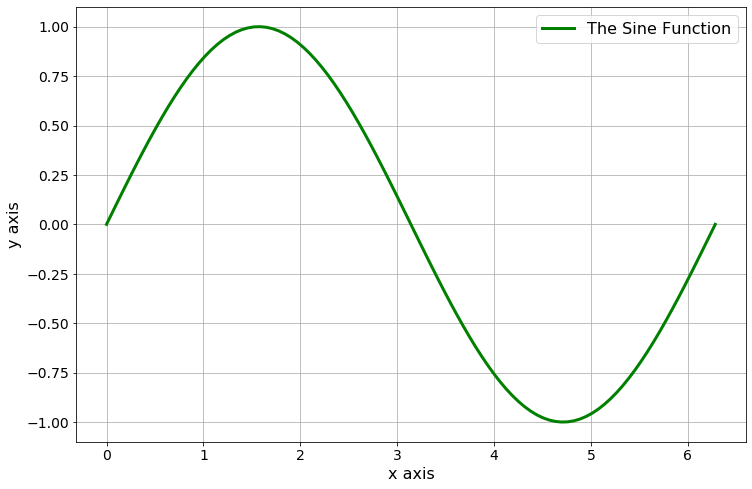
\includegraphics[width=0.75\linewidth]{images/Ch07_SineFunction} 

}

\caption{The sine function}\label{fig:unnamed-chunk-754}
\end{figure}

\begin{center}\rule{0.5\linewidth}{0.5pt}\end{center}

\begin{example}
\protect\hypertarget{exm:unnamed-chunk-755}{}{\label{exm:unnamed-chunk-755} }Now let's do a second example, but this time we want to show four different plots on top of each other. When you start a figure, \texttt{matplotlib} is expecting all of those plots to be layered on top of each other.(Note:For MATLAB users, this means that you do not need the \texttt{hold\ on} command since it is automatically ``on''.)

In this example we will plot
\[y_0 = \sin(2\pi x) \quad y_1 = \cos(2 \pi x) \quad y_2 = y_0 + y_1 \quad \text{and} \quad y_3 = y_0 - y_1\]
on the domain \(x \in [0,1]\) with 100 equally spaced points. We'll give each of the plots a different line style, built a legend, put a grid on the plot, and give axis labels.
\end{example}

\begin{Shaded}
\begin{Highlighting}[]
\ImportTok{import}\NormalTok{ numpy }\ImportTok{as}\NormalTok{ np}
\ImportTok{import}\NormalTok{ matplotlib.pyplot }\ImportTok{as}\NormalTok{ plt}
\CommentTok{\# \%matplotlib inline \# you may need this in Jupyter Notebooks}

\CommentTok{\# build the x and y values}
\NormalTok{x }\OperatorTok{=}\NormalTok{ np.linspace(}\DecValTok{0}\NormalTok{,}\DecValTok{1}\NormalTok{,}\DecValTok{100}\NormalTok{)}
\NormalTok{y0 }\OperatorTok{=}\NormalTok{ np.sin(}\DecValTok{2}\OperatorTok{*}\NormalTok{np.pi}\OperatorTok{*}\NormalTok{x)}
\NormalTok{y1 }\OperatorTok{=}\NormalTok{ np.cos(}\DecValTok{2}\OperatorTok{*}\NormalTok{np.pi}\OperatorTok{*}\NormalTok{x)}
\NormalTok{y2 }\OperatorTok{=}\NormalTok{ y0 }\OperatorTok{+}\NormalTok{ y1}
\NormalTok{y3 }\OperatorTok{=}\NormalTok{ y0 }\OperatorTok{{-}}\NormalTok{ y1}

\CommentTok{\# plot each of the functions (notice that they will be on the same axes)}
\NormalTok{plt.plot(x, y0, }\StringTok{\textquotesingle{}b{-}.\textquotesingle{}}\NormalTok{, label}\OperatorTok{=}\VerbatimStringTok{r"$y\_0 = \textbackslash{}sin(2\textbackslash{}pi x)$"}\NormalTok{)}
\NormalTok{plt.plot(x, y1, }\StringTok{\textquotesingle{}r{-}{-}\textquotesingle{}}\NormalTok{, label}\OperatorTok{=}\VerbatimStringTok{r"$y\_1 = \textbackslash{}cos(2\textbackslash{}pi x)$"}\NormalTok{)}
\NormalTok{plt.plot(x, y2, }\StringTok{\textquotesingle{}g:\textquotesingle{}}\NormalTok{, label}\OperatorTok{=}\VerbatimStringTok{r"$y\_2 = y\_0 + y\_1$"}\NormalTok{)}
\NormalTok{plt.plot(x, y3, }\StringTok{\textquotesingle{}k{-}\textquotesingle{}}\NormalTok{, label}\OperatorTok{=}\VerbatimStringTok{r"$y\_3 = y\_0 {-} y\_1$"}\NormalTok{)}

\CommentTok{\# put in a grid, legend, title, and axis labels}
\NormalTok{plt.grid()}
\NormalTok{plt.legend()}
\NormalTok{plt.title(}\StringTok{"Awesome Title"}\NormalTok{)}
\NormalTok{plt.xlabel(}\StringTok{\textquotesingle{}x axis label\textquotesingle{}}\NormalTok{)}
\NormalTok{plt.ylabel(}\StringTok{\textquotesingle{}y axis label\textquotesingle{}}\NormalTok{)}
\NormalTok{plt.show()}
\end{Highlighting}
\end{Shaded}

\begin{figure}

{\centering 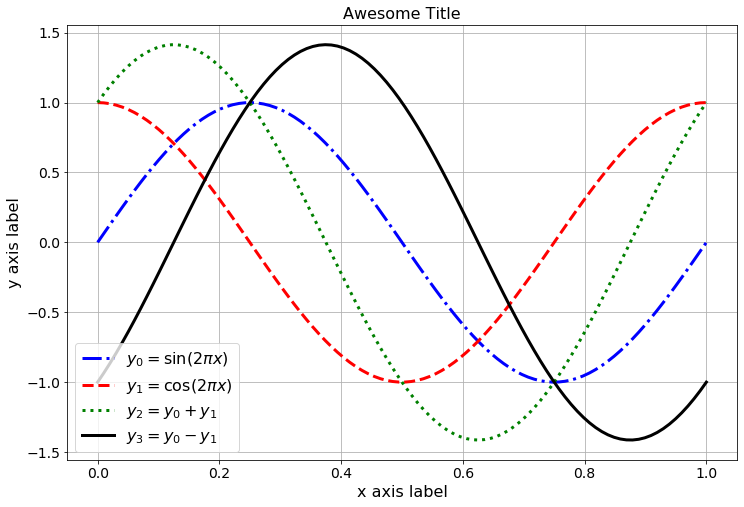
\includegraphics[width=0.75\linewidth]{images/Ch07_SeveralSines} 

}

\caption{Plots of the sine, cosine, and sums and differences.}\label{fig:unnamed-chunk-757}
\end{figure}

Notice that the legend was placed automatically. There are ways to control the placement of the legend if you wish, but for now just let Python and \texttt{matplotlib} have control over the placement.

\begin{center}\rule{0.5\linewidth}{0.5pt}\end{center}

\begin{example}
\protect\hypertarget{exm:unnamed-chunk-758}{}{\label{exm:unnamed-chunk-758} }Now let's create the same plot with slightly different code. The \texttt{plot} command can take several \((x, y)\) pairs in the same line of code. This can really shrink the amount of coding that you have to do when plotting several functions on top of each other.
\end{example}

\begin{Shaded}
\begin{Highlighting}[]
\CommentTok{\# The next line of code does all of the plotting of all of the functions.}
\CommentTok{\# Notice the order: x, y, color and line style, repeat}
\ImportTok{import}\NormalTok{ numpy }\ImportTok{as}\NormalTok{ np}
\ImportTok{import}\NormalTok{ matplotlib.pyplot }\ImportTok{as}\NormalTok{ plt}
\NormalTok{x }\OperatorTok{=}\NormalTok{ np.linspace(}\DecValTok{0}\NormalTok{,}\DecValTok{1}\NormalTok{,}\DecValTok{100}\NormalTok{)}
\NormalTok{y0 }\OperatorTok{=}\NormalTok{ np.sin(}\DecValTok{2}\OperatorTok{*}\NormalTok{np.pi}\OperatorTok{*}\NormalTok{x)}
\NormalTok{y1 }\OperatorTok{=}\NormalTok{ np.cos(}\DecValTok{2}\OperatorTok{*}\NormalTok{np.pi}\OperatorTok{*}\NormalTok{x)}
\NormalTok{y2 }\OperatorTok{=}\NormalTok{ y0 }\OperatorTok{+}\NormalTok{ y1}
\NormalTok{y3 }\OperatorTok{=}\NormalTok{ y0 }\OperatorTok{{-}}\NormalTok{ y1}
\NormalTok{plt.plot(x, y0, }\StringTok{\textquotesingle{}b{-}.\textquotesingle{}}\NormalTok{, x, y1, }\StringTok{\textquotesingle{}r{-}{-}\textquotesingle{}}\NormalTok{, x, y2, }\StringTok{\textquotesingle{}g:\textquotesingle{}}\NormalTok{, x, y3, }\StringTok{\textquotesingle{}k{-}\textquotesingle{}}\NormalTok{)}

\NormalTok{plt.grid()}
\NormalTok{plt.legend([}\VerbatimStringTok{r"$y\_0 = \textbackslash{}sin(2\textbackslash{}pi x)$"}\NormalTok{,}\VerbatimStringTok{r"$y\_1 = \textbackslash{}cos(2\textbackslash{}pi x)$"}\NormalTok{,}\OperatorTok{\textbackslash{}}
            \VerbatimStringTok{r"$y\_2 = y\_0 + y\_1$"}\NormalTok{,}\VerbatimStringTok{r"$y\_3 = y\_0 {-} y\_1$"}\NormalTok{])}
\NormalTok{plt.title(}\StringTok{"Awesome Title"}\NormalTok{)}
\NormalTok{plt.xlabel(}\StringTok{\textquotesingle{}x axis label\textquotesingle{}}\NormalTok{)}
\NormalTok{plt.ylabel(}\StringTok{\textquotesingle{}y axis label\textquotesingle{}}\NormalTok{)}
\NormalTok{plt.show()}
\end{Highlighting}
\end{Shaded}

\begin{figure}

{\centering 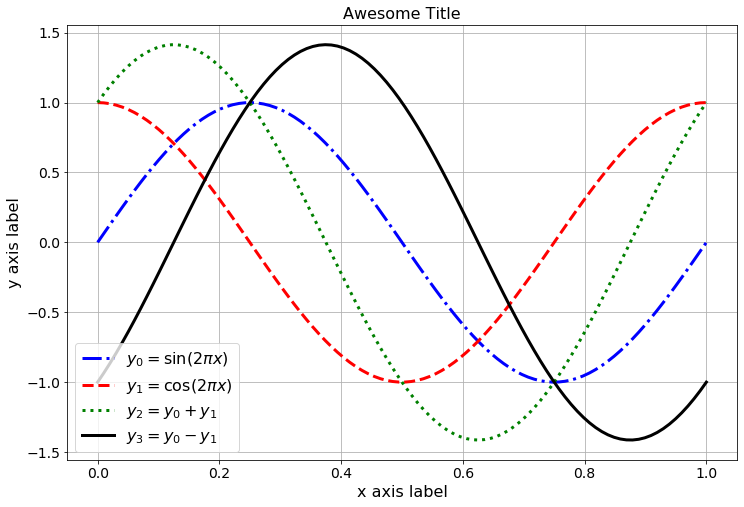
\includegraphics[width=0.75\linewidth]{images/Ch07_SeveralSines2} 

}

\caption{A second plot of the sine, cosine, and sums and differences.}\label{fig:unnamed-chunk-760}
\end{figure}

\begin{center}\rule{0.5\linewidth}{0.5pt}\end{center}

\begin{exercise}
\protect\hypertarget{exr:unnamed-chunk-761}{}{\label{exr:unnamed-chunk-761} }Plot the functions \(f(x) = x^2\), \(g(x) = x^3\), and \(h(x) = x^4\) on the same axes. Use the domain \(x \in [0,1]\) and the range \(y \in [0,1]\). Put a grid, a legend, a title, and appropriate labels on the axes.
\end{exercise}

\begin{center}\rule{0.5\linewidth}{0.5pt}\end{center}

\hypertarget{subplots}{%
\subsection{Subplots}\label{subplots}}

It is often very handy to place plots side-by-side or as some array of plots. The \texttt{subplots} command allows us that control. The main idea is that we are setting up a matrix of blank plots and then populating the axes with the plots that we want.

\begin{center}\rule{0.5\linewidth}{0.5pt}\end{center}

\begin{example}
\protect\hypertarget{exm:unnamed-chunk-762}{}{\label{exm:unnamed-chunk-762} }Let's repeat the previous exercise, but this time we will put each of the plots in its own subplot. There are a few extra coding quirks that come along with building subplots so we'll highlight each block of code separately.

\begin{itemize}
\tightlist
\item
  First we set up the plot area with \texttt{plt.subplots()}. The first two inputs to the \texttt{subplots} command are the number of rows and the number of columns in your plot array. For the first example we will do 2 rows of plots with 2 columns -- so there are four plots total. The last input for the \texttt{subplots} command is the size of the figure (this is really just so that it shows up well in Jupyter Notebooks -- spend some time playing with the figure size to get it to look right).
\item
  Then we build each plot individually telling \texttt{matplotlib} which axes to use for each of the things in the plots.
\item
  Notice the small differences in how we set the titles and labels
\item
  In this example we are setting the \(y\)-axis to the interval \([-2,2]\) for consistency across all of the plots.
\end{itemize}
\end{example}

\begin{Shaded}
\begin{Highlighting}[]
\CommentTok{\# set up the blank matrix of plots}
\ImportTok{import}\NormalTok{ numpy }\ImportTok{as}\NormalTok{ np}
\ImportTok{import}\NormalTok{ matplotlib.pyplot }\ImportTok{as}\NormalTok{ plt}
\NormalTok{x }\OperatorTok{=}\NormalTok{ np.linspace(}\DecValTok{0}\NormalTok{,}\DecValTok{1}\NormalTok{,}\DecValTok{100}\NormalTok{)}
\NormalTok{y0 }\OperatorTok{=}\NormalTok{ np.sin(}\DecValTok{2}\OperatorTok{*}\NormalTok{np.pi}\OperatorTok{*}\NormalTok{x)}
\NormalTok{y1 }\OperatorTok{=}\NormalTok{ np.cos(}\DecValTok{2}\OperatorTok{*}\NormalTok{np.pi}\OperatorTok{*}\NormalTok{x)}
\NormalTok{y2 }\OperatorTok{=}\NormalTok{ y0 }\OperatorTok{+}\NormalTok{ y1}
\NormalTok{y3 }\OperatorTok{=}\NormalTok{ y0 }\OperatorTok{{-}}\NormalTok{ y1}

\NormalTok{fig, axes }\OperatorTok{=}\NormalTok{ plt.subplots(nrows }\OperatorTok{=} \DecValTok{2}\NormalTok{, ncols }\OperatorTok{=} \DecValTok{2}\NormalTok{, figsize }\OperatorTok{=}\NormalTok{ (}\DecValTok{10}\NormalTok{,}\DecValTok{5}\NormalTok{))}

\CommentTok{\# Build the first plot}
\NormalTok{axes[}\DecValTok{0}\NormalTok{,}\DecValTok{0}\NormalTok{].plot(x, y0, }\StringTok{\textquotesingle{}b{-}.\textquotesingle{}}\NormalTok{)}
\NormalTok{axes[}\DecValTok{0}\NormalTok{,}\DecValTok{0}\NormalTok{].grid()}
\NormalTok{axes[}\DecValTok{0}\NormalTok{,}\DecValTok{0}\NormalTok{].set\_title(}\VerbatimStringTok{r"$y\_0 = \textbackslash{}sin(2\textbackslash{}pi x)$"}\NormalTok{)}
\NormalTok{axes[}\DecValTok{0}\NormalTok{,}\DecValTok{0}\NormalTok{].set\_ylim(}\OperatorTok{{-}}\DecValTok{2}\NormalTok{,}\DecValTok{2}\NormalTok{)}
\NormalTok{axes[}\DecValTok{0}\NormalTok{,}\DecValTok{0}\NormalTok{].set\_xlabel(}\StringTok{"x"}\NormalTok{)}
\NormalTok{axes[}\DecValTok{0}\NormalTok{,}\DecValTok{0}\NormalTok{].set\_ylabel(}\StringTok{"y"}\NormalTok{)}

\CommentTok{\# Build the second plot}
\NormalTok{axes[}\DecValTok{0}\NormalTok{,}\DecValTok{1}\NormalTok{].plot(x, y1, }\StringTok{\textquotesingle{}r{-}{-}\textquotesingle{}}\NormalTok{)}
\NormalTok{axes[}\DecValTok{0}\NormalTok{,}\DecValTok{1}\NormalTok{].grid()}
\NormalTok{axes[}\DecValTok{0}\NormalTok{,}\DecValTok{1}\NormalTok{].set\_title(}\VerbatimStringTok{r"$y\_1 = \textbackslash{}cos(2\textbackslash{}pi x)$"}\NormalTok{)}
\NormalTok{axes[}\DecValTok{0}\NormalTok{,}\DecValTok{1}\NormalTok{].set\_ylim(}\OperatorTok{{-}}\DecValTok{2}\NormalTok{,}\DecValTok{2}\NormalTok{)}
\NormalTok{axes[}\DecValTok{0}\NormalTok{,}\DecValTok{1}\NormalTok{].set\_xlabel(}\StringTok{"x"}\NormalTok{)}
\NormalTok{axes[}\DecValTok{0}\NormalTok{,}\DecValTok{1}\NormalTok{].set\_ylabel(}\StringTok{"y"}\NormalTok{)}

\CommentTok{\# Build the first plot}
\NormalTok{axes[}\DecValTok{1}\NormalTok{,}\DecValTok{0}\NormalTok{].plot(x, y2, }\StringTok{\textquotesingle{}g:\textquotesingle{}}\NormalTok{)}
\NormalTok{axes[}\DecValTok{1}\NormalTok{,}\DecValTok{0}\NormalTok{].grid()}
\NormalTok{axes[}\DecValTok{1}\NormalTok{,}\DecValTok{0}\NormalTok{].set\_title(}\VerbatimStringTok{r"$y\_2 = y\_0 + y\_1$"}\NormalTok{)}
\NormalTok{axes[}\DecValTok{1}\NormalTok{,}\DecValTok{0}\NormalTok{].set\_ylim(}\OperatorTok{{-}}\DecValTok{2}\NormalTok{,}\DecValTok{2}\NormalTok{)}
\NormalTok{axes[}\DecValTok{1}\NormalTok{,}\DecValTok{0}\NormalTok{].set\_xlabel(}\StringTok{"x"}\NormalTok{)}
\NormalTok{axes[}\DecValTok{1}\NormalTok{,}\DecValTok{0}\NormalTok{].set\_ylabel(}\StringTok{"y"}\NormalTok{)}

\CommentTok{\# Build the first plot}
\NormalTok{axes[}\DecValTok{1}\NormalTok{,}\DecValTok{1}\NormalTok{].plot(x, y3, }\StringTok{\textquotesingle{}k{-}\textquotesingle{}}\NormalTok{)}
\NormalTok{axes[}\DecValTok{1}\NormalTok{,}\DecValTok{1}\NormalTok{].grid()}
\NormalTok{axes[}\DecValTok{1}\NormalTok{,}\DecValTok{1}\NormalTok{].set\_title(}\VerbatimStringTok{r"$y\_3 = y\_0 {-} y\_1$"}\NormalTok{)}
\NormalTok{axes[}\DecValTok{1}\NormalTok{,}\DecValTok{1}\NormalTok{].set\_ylim(}\OperatorTok{{-}}\DecValTok{2}\NormalTok{,}\DecValTok{2}\NormalTok{)}
\NormalTok{axes[}\DecValTok{1}\NormalTok{,}\DecValTok{1}\NormalTok{].set\_xlabel(}\StringTok{"x"}\NormalTok{)}
\NormalTok{axes[}\DecValTok{1}\NormalTok{,}\DecValTok{1}\NormalTok{].set\_ylabel(}\StringTok{"y"}\NormalTok{)}

\NormalTok{fig.tight\_layout()}
\NormalTok{plt.show()}
\end{Highlighting}
\end{Shaded}

The \texttt{fig.tight\_layout()} command makes the plot labels a bit more readable in this instance (again, something you can play with).

\begin{figure}

{\centering 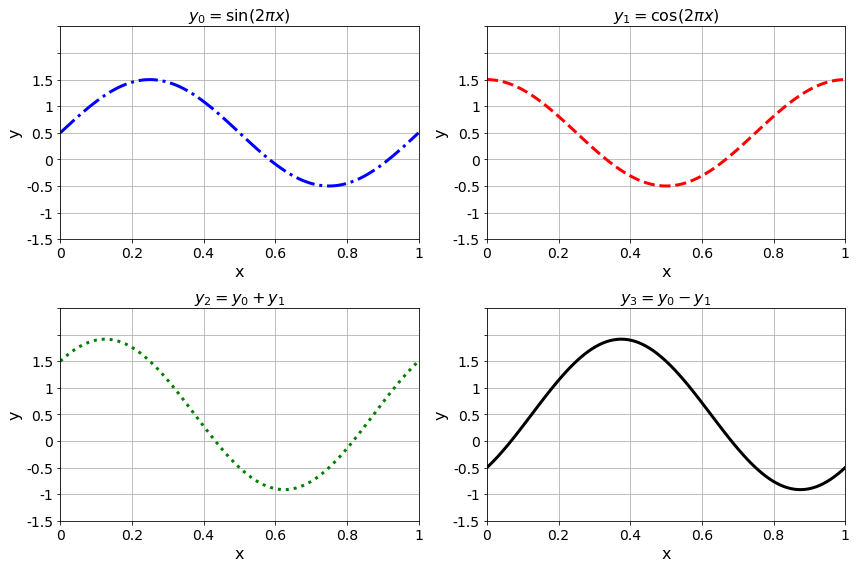
\includegraphics[width=0.75\linewidth]{images/Ch07_Subplots} 

}

\caption{An example of subplots}\label{fig:unnamed-chunk-764}
\end{figure}

\begin{center}\rule{0.5\linewidth}{0.5pt}\end{center}

\begin{exercise}
\protect\hypertarget{exr:unnamed-chunk-765}{}{\label{exr:unnamed-chunk-765} }Put the functions \(f(x) = x^2\), \(g(x) = x^3\) and \(h(x) = x^4\) in a subplot environment with 1 row and 3 columns of plots. Use the unit interval as the domain and range for all three plot, but sure that each plot has a grid, appropriate labels, an appropriate title, and the overall figure has a title.
\end{exercise}

\begin{center}\rule{0.5\linewidth}{0.5pt}\end{center}

\hypertarget{logarithmic-scaling-with-semilogy-semilogx-and-loglog}{%
\subsection{\texorpdfstring{Logarithmic Scaling with \texttt{semilogy}, \texttt{semilogx}, and \texttt{loglog}}{Logarithmic Scaling with semilogy, semilogx, and loglog}}\label{logarithmic-scaling-with-semilogy-semilogx-and-loglog}}

It is occasionally useful to scale an axis logarithmically. This arises most often when we're examining an exponential function, or some other function, that is close to zero for much of the domain. Scaling logarithmically allows us to see how small the function is getting in orders of magnitude instead of as a raw real number. We'll use this often in numerical methods.

\begin{center}\rule{0.5\linewidth}{0.5pt}\end{center}

\begin{example}
\protect\hypertarget{exm:unnamed-chunk-766}{}{\label{exm:unnamed-chunk-766} }In this example we'll plot the function \(y = 10^{-0.01x}\) on a regular (linear) scale and on a logarithmic scale on the \(y\) axis. Use the interval \([0,500]\).
\end{example}

\begin{Shaded}
\begin{Highlighting}[]
\ImportTok{import}\NormalTok{ numpy }\ImportTok{as}\NormalTok{ np}
\ImportTok{import}\NormalTok{ matplotlib.pyplot }\ImportTok{as}\NormalTok{ plt}
\NormalTok{x }\OperatorTok{=}\NormalTok{ np.linspace(}\DecValTok{0}\NormalTok{,}\DecValTok{500}\NormalTok{,}\DecValTok{1000}\NormalTok{)}
\NormalTok{y }\OperatorTok{=} \DecValTok{10}\OperatorTok{**}\NormalTok{(}\OperatorTok{{-}}\FloatTok{0.01}\OperatorTok{*}\NormalTok{x)}
\NormalTok{fig, axis }\OperatorTok{=}\NormalTok{ plt.subplots(}\DecValTok{1}\NormalTok{,}\DecValTok{2}\NormalTok{, figsize }\OperatorTok{=}\NormalTok{ (}\DecValTok{10}\NormalTok{,}\DecValTok{5}\NormalTok{))}

\NormalTok{axis[}\DecValTok{0}\NormalTok{].plot(x,y, }\StringTok{\textquotesingle{}r\textquotesingle{}}\NormalTok{)}
\NormalTok{axis[}\DecValTok{0}\NormalTok{].grid()}
\NormalTok{axis[}\DecValTok{0}\NormalTok{].set\_title(}\StringTok{"Linearly scaled y axis"}\NormalTok{)}
\NormalTok{axis[}\DecValTok{0}\NormalTok{].set\_xlabel(}\StringTok{"x"}\NormalTok{)}
\NormalTok{axis[}\DecValTok{0}\NormalTok{].set\_ylabel(}\StringTok{"y"}\NormalTok{)}

\NormalTok{axis[}\DecValTok{1}\NormalTok{].semilogy(x,y, }\StringTok{\textquotesingle{}k{-}{-}\textquotesingle{}}\NormalTok{)}
\NormalTok{axis[}\DecValTok{1}\NormalTok{].grid()}
\NormalTok{axis[}\DecValTok{1}\NormalTok{].set\_title(}\StringTok{"Logarithmically scaled y axis"}\NormalTok{)}
\NormalTok{axis[}\DecValTok{1}\NormalTok{].set\_xlabel(}\StringTok{"x"}\NormalTok{)}
\NormalTok{axis[}\DecValTok{1}\NormalTok{].set\_ylabel(}\StringTok{"Log(y)"}\NormalTok{)}
\NormalTok{plt.show()}
\end{Highlighting}
\end{Shaded}

It should be noted that the same result can be achieved using the \texttt{yscale} command along with the \texttt{plot} command instead of using the \texttt{semilogy} command. Pay careful attention to the subtle changes in the following code.

\begin{Shaded}
\begin{Highlighting}[]
\ImportTok{import}\NormalTok{ numpy }\ImportTok{as}\NormalTok{ np}
\ImportTok{import}\NormalTok{ matplotlib.pyplot }\ImportTok{as}\NormalTok{ plt}
\NormalTok{x }\OperatorTok{=}\NormalTok{ np.linspace(}\DecValTok{0}\NormalTok{,}\DecValTok{500}\NormalTok{,}\DecValTok{1000}\NormalTok{)}
\NormalTok{y }\OperatorTok{=} \DecValTok{10}\OperatorTok{**}\NormalTok{(}\OperatorTok{{-}}\FloatTok{0.01}\OperatorTok{*}\NormalTok{x)}
\NormalTok{fig, axis }\OperatorTok{=}\NormalTok{ plt.subplots(}\DecValTok{1}\NormalTok{,}\DecValTok{2}\NormalTok{, figsize }\OperatorTok{=}\NormalTok{ (}\DecValTok{10}\NormalTok{,}\DecValTok{5}\NormalTok{))}

\NormalTok{axis[}\DecValTok{0}\NormalTok{].plot(x,y, }\StringTok{\textquotesingle{}r\textquotesingle{}}\NormalTok{)}
\NormalTok{axis[}\DecValTok{0}\NormalTok{].grid()}
\NormalTok{axis[}\DecValTok{0}\NormalTok{].set\_title(}\StringTok{"Linearly scaled y axis"}\NormalTok{)}
\NormalTok{axis[}\DecValTok{0}\NormalTok{].set\_xlabel(}\StringTok{"x"}\NormalTok{)}
\NormalTok{axis[}\DecValTok{0}\NormalTok{].set\_ylabel(}\StringTok{"y"}\NormalTok{)}

\NormalTok{axis[}\DecValTok{1}\NormalTok{].plot(x,y, }\StringTok{\textquotesingle{}k{-}{-}\textquotesingle{}}\NormalTok{) }\CommentTok{\# \textless{}{-}{-}{-}{-}{-} Notice the change here}
\NormalTok{axis[}\DecValTok{1}\NormalTok{].set\_yscale(}\StringTok{"log"}\NormalTok{) }\CommentTok{\# \textless{}{-}{-}{-}{-}{-} And we added this line}
\NormalTok{axis[}\DecValTok{1}\NormalTok{].grid()}
\NormalTok{axis[}\DecValTok{1}\NormalTok{].set\_title(}\StringTok{"Logarithmically scaled y axis"}\NormalTok{)}
\NormalTok{axis[}\DecValTok{1}\NormalTok{].set\_xlabel(}\StringTok{"x"}\NormalTok{)}
\NormalTok{axis[}\DecValTok{1}\NormalTok{].set\_ylabel(}\StringTok{"Log(y)"}\NormalTok{)}
\end{Highlighting}
\end{Shaded}

\begin{figure}

{\centering 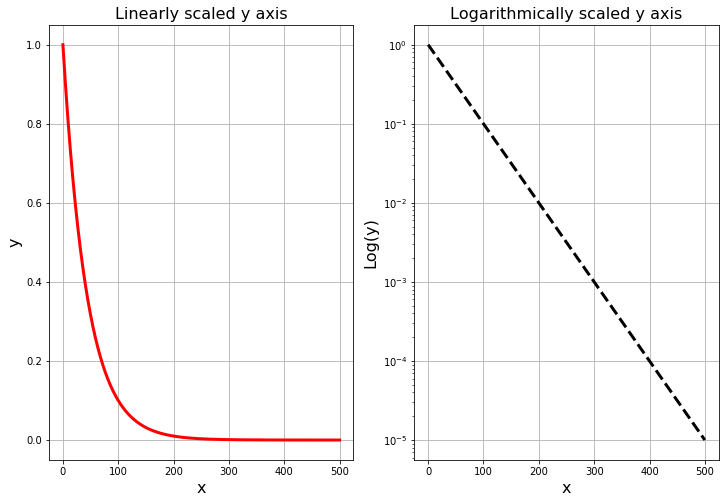
\includegraphics[width=0.75\linewidth]{images/Ch07_LogScale} 

}

\caption{An example of using logarithmic scaling.}\label{fig:unnamed-chunk-769}
\end{figure}

\begin{center}\rule{0.5\linewidth}{0.5pt}\end{center}

\begin{exercise}
\protect\hypertarget{exr:unnamed-chunk-770}{}{\label{exr:unnamed-chunk-770} }Plot the function \(f(x) = x^3\) for \(x \in [0,1]\) on linearly scaled axes, logarithmic axis in the \(y\) direction, logarithmically scaled axes in the \(x\) direction, and a log-log plot with logarithmic scaling on both axes. Use \texttt{subplots} to put your plots side-by-side. Give appropriate labels, titles, etc.
\end{exercise}

\begin{center}\rule{0.5\linewidth}{0.5pt}\end{center}

\hypertarget{symbolic-python-with-sympy}{%
\section{\texorpdfstring{Symbolic Python with \texttt{sympy}}{Symbolic Python with sympy}}\label{symbolic-python-with-sympy}}

In this section we will learn the tools necessary to do symbolic mathematics in Python. The relevant package is \texttt{sympy} (symbolic Python) and it works much like Mathematica, Maple, or MATLAB's symbolic toolbox. That being said, Mathematica and Maple are designed to do symbolic computation in the fastest and best possible ways, so in some sense, \texttt{sympy} is a little step-sibling to these much bigger pieces of software. Remember: Python is free, and this is a book on numerical analysis -- we will not be doing much symbolic work in this particular class, but these tools do occasionally come in handy.

Let's import \texttt{sympy} in the usual way. We will use the nickname \texttt{sp} (just like we used \texttt{np} for \texttt{numpy}). This is not a standard nickname in the Python literature, but it will suffice for our purposes.

\begin{center}\rule{0.5\linewidth}{0.5pt}\end{center}

\begin{exercise}
\protect\hypertarget{exr:unnamed-chunk-771}{}{\label{exr:unnamed-chunk-771} }Load \texttt{sympy} and use the \texttt{dir()} command to see what functions are inside the \texttt{sympy} library.
\end{exercise}

\begin{center}\rule{0.5\linewidth}{0.5pt}\end{center}

\begin{example}
\protect\hypertarget{exm:unnamed-chunk-772}{}{\label{exm:unnamed-chunk-772} }If you include the command \texttt{sp.init\_printing()} after you load \texttt{sympy} you will get some nice LaTeX style output in your Jupyter Notebooks.
\end{example}

\begin{center}\rule{0.5\linewidth}{0.5pt}\end{center}

\hypertarget{symbolic-variables-with-symbols}{%
\subsection{\texorpdfstring{Symbolic Variables with \texttt{symbols}}{Symbolic Variables with symbols}}\label{symbolic-variables-with-symbols}}

When you are working with symbolic variables you have to tell Python that that's what you're doing. In other words, we actually have to type-cast the variables when we name them. Otherwise Python won't know what to do with them -- we need to explicitly tell it that we are working with symbols!

\begin{center}\rule{0.5\linewidth}{0.5pt}\end{center}

\begin{example}
\protect\hypertarget{exm:unnamed-chunk-773}{}{\label{exm:unnamed-chunk-773} }Let's define the variable \(x\) as a symbolic variable. Then we'll define a few symbolic expressions that use \(x\) as a variable.
\end{example}

\begin{Shaded}
\begin{Highlighting}[]
\ImportTok{import}\NormalTok{ sympy }\ImportTok{as}\NormalTok{ sp}
\NormalTok{x }\OperatorTok{=}\NormalTok{ sp.Symbol(}\StringTok{\textquotesingle{}x\textquotesingle{}}\NormalTok{) }\CommentTok{\# note the capitalization}
\end{Highlighting}
\end{Shaded}

Now we'll define the function \(f(x) = (x+2)^3\) and spend the next few
examples playing with it.

\begin{Shaded}
\begin{Highlighting}[]
\NormalTok{f }\OperatorTok{=}\NormalTok{ (x}\OperatorTok{+}\DecValTok{2}\NormalTok{)}\OperatorTok{**}\DecValTok{3} \CommentTok{\# A symbolic function}
\BuiltInTok{print}\NormalTok{(f)}
\end{Highlighting}
\end{Shaded}

\begin{verbatim}
## (x + 2)**3
\end{verbatim}

Notice that the output of these lines of code is not necessarily very nicely formatted as a symbolic expression. What we would really want to see is \(\displaystyle (x+2)^3\). If you include the code \texttt{sp.init\_printing()} after you import the \texttt{sympy} library then you should get nice LaTeX style formatting in your answers.

\begin{center}\rule{0.5\linewidth}{0.5pt}\end{center}

\begin{example}
\protect\hypertarget{exm:unnamed-chunk-776}{}{\label{exm:unnamed-chunk-776} }Be careful that you are using symbolically defined function along with your symbols. For example, see the code below:
\end{example}

\begin{Shaded}
\begin{Highlighting}[]
\CommentTok{\# this line gives an error since it doesn\textquotesingle{}t know which "sine" to use.}
\NormalTok{g }\OperatorTok{=}\NormalTok{ sin(x) }
\end{Highlighting}
\end{Shaded}

\begin{Shaded}
\begin{Highlighting}[]
\ImportTok{import}\NormalTok{ sympy }\ImportTok{as}\NormalTok{ sp}
\NormalTok{x }\OperatorTok{=}\NormalTok{ sp.Symbol(}\StringTok{\textquotesingle{}x\textquotesingle{}}\NormalTok{)}
\NormalTok{g }\OperatorTok{=}\NormalTok{ sp.sin(x) }\CommentTok{\# this one works}
\BuiltInTok{print}\NormalTok{(g)}
\end{Highlighting}
\end{Shaded}

\begin{verbatim}
## sin(x)
\end{verbatim}

\begin{center}\rule{0.5\linewidth}{0.5pt}\end{center}

\hypertarget{symbolic-algebra}{%
\subsection{Symbolic Algebra}\label{symbolic-algebra}}

One of the primary purposes of doing symbolic programming is to do symbolic algebra (the other is typically symbolic calculus). In this section we'll look at a few of the common algebraic exercises that can be handled with \texttt{sympy}.

\begin{center}\rule{0.5\linewidth}{0.5pt}\end{center}

\begin{example}[symbolic expand]
\protect\hypertarget{exm:unnamed-chunk-779}{}{\label{exm:unnamed-chunk-779} \iffalse (symbolic expand) \fi{} }Expand the function \(f(x) = (x+2)^3\). In other words, multiply this out fully so that it is a sum or difference of monomials instead of the cube of a binomial.
\end{example}

\begin{Shaded}
\begin{Highlighting}[]
\ImportTok{import}\NormalTok{ sympy }\ImportTok{as}\NormalTok{ sp}
\NormalTok{x }\OperatorTok{=}\NormalTok{ sp.Symbol(}\StringTok{\textquotesingle{}x\textquotesingle{}}\NormalTok{)}
\NormalTok{f }\OperatorTok{=}\NormalTok{ (x}\OperatorTok{+}\DecValTok{2}\NormalTok{)}\OperatorTok{**}\DecValTok{3}
\NormalTok{sp.expand(f) }\CommentTok{\# do the multiplication to expand the polynomial}
\end{Highlighting}
\end{Shaded}

\begin{verbatim}
## x**3 + 6*x**2 + 12*x + 8
\end{verbatim}

\begin{center}\rule{0.5\linewidth}{0.5pt}\end{center}

\begin{example}[symbolic factoring]
\protect\hypertarget{exm:unnamed-chunk-781}{}{\label{exm:unnamed-chunk-781} \iffalse (symbolic factoring) \fi{} }We will factor the polynomial \(h(x) = x^2 + 4x + 3\).
\end{example}

\begin{Shaded}
\begin{Highlighting}[]
\ImportTok{import}\NormalTok{ sympy }\ImportTok{as}\NormalTok{ sp}
\NormalTok{x }\OperatorTok{=}\NormalTok{ sp.Symbol(}\StringTok{\textquotesingle{}x\textquotesingle{}}\NormalTok{)}
\NormalTok{h }\OperatorTok{=}\NormalTok{ x}\OperatorTok{**}\DecValTok{2} \OperatorTok{+} \DecValTok{4}\OperatorTok{*}\NormalTok{x }\OperatorTok{+} \DecValTok{3}
\NormalTok{sp.factor(h) }\CommentTok{\# factor this polynomial}
\end{Highlighting}
\end{Shaded}

\begin{verbatim}
## (x + 1)*(x + 3)
\end{verbatim}

\begin{center}\rule{0.5\linewidth}{0.5pt}\end{center}

\begin{example}[Trigonometric Simplification]
\protect\hypertarget{exm:unnamed-chunk-783}{}{\label{exm:unnamed-chunk-783} \iffalse (Trigonometric Simplification) \fi{} }The \texttt{sympy} package knows how to work with trigonometric identities. In this example we show how \texttt{sympy} expands \(\sin(a+b)\).
\end{example}

\begin{Shaded}
\begin{Highlighting}[]
\ImportTok{import}\NormalTok{ sympy }\ImportTok{as}\NormalTok{ sp}
\NormalTok{a, b }\OperatorTok{=}\NormalTok{ sp.symbols(}\StringTok{\textquotesingle{}a b\textquotesingle{}}\NormalTok{)}
\NormalTok{j }\OperatorTok{=}\NormalTok{ sp.sin(a}\OperatorTok{+}\NormalTok{b)}
\NormalTok{sp.expand(j, trig}\OperatorTok{=}\VariableTok{True}\NormalTok{) }\CommentTok{\# Trig identities are built in!}
\end{Highlighting}
\end{Shaded}

\begin{verbatim}
## sin(a)*cos(b) + sin(b)*cos(a)
\end{verbatim}

\begin{center}\rule{0.5\linewidth}{0.5pt}\end{center}

\begin{example}[Symbolic Simplification]
\protect\hypertarget{exm:unnamed-chunk-785}{}{\label{exm:unnamed-chunk-785} \iffalse (Symbolic Simplification) \fi{} }In this example we will simplify the function \(g(x) = x^3 + 5x^3 + 12x^2 +1\).
\end{example}

\begin{Shaded}
\begin{Highlighting}[]
\ImportTok{import}\NormalTok{ sympy }\ImportTok{as}\NormalTok{ sp}
\NormalTok{x }\OperatorTok{=}\NormalTok{ sp.Symbol(}\StringTok{\textquotesingle{}x\textquotesingle{}}\NormalTok{)}
\NormalTok{g }\OperatorTok{=}\NormalTok{ x}\OperatorTok{**}\DecValTok{3} \OperatorTok{+} \DecValTok{5}\OperatorTok{*}\NormalTok{x}\OperatorTok{**}\DecValTok{3} \OperatorTok{+} \DecValTok{12}\OperatorTok{*}\NormalTok{x}\OperatorTok{**}\DecValTok{2} \OperatorTok{+} \DecValTok{1}
\NormalTok{sp.simplify(g) }\CommentTok{\# Simplify some algebraic expression}
\end{Highlighting}
\end{Shaded}

\begin{verbatim}
## 6*x**3 + 12*x**2 + 1
\end{verbatim}

\begin{center}\rule{0.5\linewidth}{0.5pt}\end{center}

\begin{example}
\protect\hypertarget{exm:unnamed-chunk-787}{}{\label{exm:unnamed-chunk-787} }In this example we'll simplify an expression that involves trigonometry.
\end{example}

\begin{Shaded}
\begin{Highlighting}[]
\ImportTok{import}\NormalTok{ sympy }\ImportTok{as}\NormalTok{ sp}
\NormalTok{x }\OperatorTok{=}\NormalTok{ sp.Symbol(}\StringTok{\textquotesingle{}x\textquotesingle{}}\NormalTok{)}
\NormalTok{sp.simplify( sp.sin(x) }\OperatorTok{/}\NormalTok{ sp.cos(x)) }\CommentTok{\# simplify a trig expression.}
\end{Highlighting}
\end{Shaded}

\begin{verbatim}
## tan(x)
\end{verbatim}

\begin{center}\rule{0.5\linewidth}{0.5pt}\end{center}

\begin{example}[Symbolic Equation Solving]
\protect\hypertarget{exm:unnamed-chunk-789}{}{\label{exm:unnamed-chunk-789} \iffalse (Symbolic Equation Solving) \fi{} }The primary goal of many algebra problems is to solve an equation. We will dedicate more time to algebraic equation solving later in this section, but this example gives a simple example of how it works in \texttt{sympy}.

We want to solve the equation \(x^2 + 4x + 3 = 0\) for \(x\).
\end{example}

\begin{Shaded}
\begin{Highlighting}[]
\ImportTok{import}\NormalTok{ sympy }\ImportTok{as}\NormalTok{ sp}
\NormalTok{x }\OperatorTok{=}\NormalTok{ sp.Symbol(}\StringTok{\textquotesingle{}x\textquotesingle{}}\NormalTok{)}
\NormalTok{h }\OperatorTok{=}\NormalTok{ x}\OperatorTok{**}\DecValTok{2} \OperatorTok{+} \DecValTok{4}\OperatorTok{*}\NormalTok{x }\OperatorTok{+} \DecValTok{3}
\NormalTok{sp.solve(h,x)}
\end{Highlighting}
\end{Shaded}

\begin{verbatim}
## [-3, -1]
\end{verbatim}

As expected, the roots of the function \(h(x)\) are \(x=-3\) and \(x=1\) since \(h(x)\) factors into \(h(x) = (x+3)(x-1)\).

\begin{center}\rule{0.5\linewidth}{0.5pt}\end{center}

\hypertarget{symbolic-function-evaluation}{%
\subsection{Symbolic Function Evaluation}\label{symbolic-function-evaluation}}

In \texttt{sympy} we cannot simply just evaluate functions as we would on paper. Let's say we have the function \(f(x)= (x+2)^3\) and we want to find \(f(5)\). We would say that we ``substitute 5 into f for x'', and that is exactly what we have to tell Python. Unfortunately we cannot just write \texttt{f(5)} since that would mean that \texttt{f} is a Python function and we are sending the number 5 into that function. This is an unfortunate double-use of the word ``function'', but stop and think about it for a second: When we write \texttt{f\ =\ (x+2)**3} we are just telling Python that \texttt{f} is a symbolic expression in terms of the symbol \texttt{x}, but we did not use \texttt{def} to define it as a function as we did for all other function.

\begin{center}\rule{0.5\linewidth}{0.5pt}\end{center}

\begin{example}
\protect\hypertarget{exm:unnamed-chunk-791}{}{\label{exm:unnamed-chunk-791} }The following code is what the mathematicians in us would like to do:
\end{example}

\begin{Shaded}
\begin{Highlighting}[]
\ImportTok{import}\NormalTok{ sympy }\ImportTok{as}\NormalTok{ sp}
\NormalTok{x }\OperatorTok{=}\NormalTok{ sp.Symbol(}\StringTok{\textquotesingle{}x\textquotesingle{}}\NormalTok{)}
\NormalTok{f }\OperatorTok{=}\NormalTok{ (x}\OperatorTok{+}\DecValTok{2}\NormalTok{)}\OperatorTok{**}\DecValTok{3}
\NormalTok{f(}\DecValTok{5}\NormalTok{) }\CommentTok{\# This gives an error!}
\end{Highlighting}
\end{Shaded}

\ldots{} but this is how it should be done:

\begin{Shaded}
\begin{Highlighting}[]
\ImportTok{import}\NormalTok{ sympy }\ImportTok{as}\NormalTok{ sp}
\NormalTok{x }\OperatorTok{=}\NormalTok{ sp.Symbol(}\StringTok{\textquotesingle{}x\textquotesingle{}}\NormalTok{)}
\NormalTok{f }\OperatorTok{=}\NormalTok{ (x}\OperatorTok{+}\DecValTok{2}\NormalTok{)}\OperatorTok{**}\DecValTok{3}
\NormalTok{f.subs(x,}\DecValTok{5}\NormalTok{) }\CommentTok{\# This actually substitutes 5 for x in f}
\end{Highlighting}
\end{Shaded}

\begin{verbatim}
## 343
\end{verbatim}

\begin{center}\rule{0.5\linewidth}{0.5pt}\end{center}

\hypertarget{symbolic-calculus}{%
\subsection{Symbolic Calculus}\label{symbolic-calculus}}

The \texttt{sympy} package has routines to take symbolic derivatives, antiderivatives, limits, and Taylor series just like other computer algebra systems.

\hypertarget{derivatives}{%
\subsubsection{Derivatives}\label{derivatives}}

The \texttt{diff} command in \texttt{sympy} does differentiation: \texttt{sp.diff(function,\ variable,\ {[}order{]})}.

Take careful note that \texttt{diff} is defined both in \texttt{sympy} and in \texttt{numpy}. That means that there are symbolic and numerical routines for taking derivatives in Python \ldots and we need to tell our instance of Python which one we're working with every time we use it.

\begin{center}\rule{0.5\linewidth}{0.5pt}\end{center}

\begin{example}[Symbolic Differentiation]
\protect\hypertarget{exm:unnamed-chunk-794}{}{\label{exm:unnamed-chunk-794} \iffalse (Symbolic Differentiation) \fi{} }In this example we'll differentiate the function \(f(x) = (x+2)^3\).
\end{example}

\begin{Shaded}
\begin{Highlighting}[]
\ImportTok{import}\NormalTok{ sympy }\ImportTok{as}\NormalTok{ sp }
\NormalTok{x }\OperatorTok{=}\NormalTok{ sp.Symbol(}\StringTok{\textquotesingle{}x\textquotesingle{}}\NormalTok{) }\CommentTok{\# Define the symbol x}
\NormalTok{f }\OperatorTok{=}\NormalTok{ (x}\OperatorTok{+}\DecValTok{2}\NormalTok{)}\OperatorTok{**}\DecValTok{3} \CommentTok{\# Define a symbolic function f(x) = (x+2)\^{}3}
\NormalTok{df }\OperatorTok{=}\NormalTok{ sp.diff(f,x) }\CommentTok{\# Take the derivative of f and call it "df"}
\BuiltInTok{print}\NormalTok{(}\StringTok{"f(x) = "}\NormalTok{, f)}
\end{Highlighting}
\end{Shaded}

\begin{verbatim}
## f(x) =  (x + 2)**3
\end{verbatim}

\begin{Shaded}
\begin{Highlighting}[]
\BuiltInTok{print}\NormalTok{(}\StringTok{"f\textquotesingle{}(x) = "}\NormalTok{,df)}
\end{Highlighting}
\end{Shaded}

\begin{verbatim}
## f'(x) =  3*(x + 2)**2
\end{verbatim}

\begin{Shaded}
\begin{Highlighting}[]
\BuiltInTok{print}\NormalTok{(}\StringTok{"f\textquotesingle{}(x) = "}\NormalTok{, sp.expand(df))}
\end{Highlighting}
\end{Shaded}

\begin{verbatim}
## f'(x) =  3*x**2 + 12*x + 12
\end{verbatim}

\begin{center}\rule{0.5\linewidth}{0.5pt}\end{center}

\begin{example}
\protect\hypertarget{exm:unnamed-chunk-796}{}{\label{exm:unnamed-chunk-796} }Now let's get the first, second, third, and fourth derivatives of the
function \texttt{f}.
\end{example}

\begin{Shaded}
\begin{Highlighting}[]
\ImportTok{import}\NormalTok{ sympy }\ImportTok{as}\NormalTok{ sp }
\NormalTok{x }\OperatorTok{=}\NormalTok{ sp.Symbol(}\StringTok{\textquotesingle{}x\textquotesingle{}}\NormalTok{) }\CommentTok{\# Define the symbol x}
\NormalTok{f }\OperatorTok{=}\NormalTok{ (x}\OperatorTok{+}\DecValTok{2}\NormalTok{)}\OperatorTok{**}\DecValTok{3} \CommentTok{\# Define a symbolic function f(x) = (x+2)\^{}3}
\NormalTok{df }\OperatorTok{=}\NormalTok{ sp.diff(f,x,}\DecValTok{1}\NormalTok{) }\CommentTok{\# first derivative}
\NormalTok{ddf }\OperatorTok{=}\NormalTok{ sp.diff(f,x,}\DecValTok{2}\NormalTok{) }\CommentTok{\# second deriative}
\NormalTok{dddf }\OperatorTok{=}\NormalTok{ sp.diff(f,x,}\DecValTok{3}\NormalTok{) }\CommentTok{\# third deriative}
\NormalTok{ddddf }\OperatorTok{=}\NormalTok{ sp.diff(f,x,}\DecValTok{4}\NormalTok{) }\CommentTok{\# fourth deriative}
\BuiltInTok{print}\NormalTok{(}\StringTok{"f\textquotesingle{}(x) = "}\NormalTok{,df)}
\end{Highlighting}
\end{Shaded}

\begin{verbatim}
## f'(x) =  3*(x + 2)**2
\end{verbatim}

\begin{Shaded}
\begin{Highlighting}[]
\BuiltInTok{print}\NormalTok{(}\StringTok{"f\textquotesingle{}\textquotesingle{}(x) = "}\NormalTok{,sp.simplify(ddf))}
\end{Highlighting}
\end{Shaded}

\begin{verbatim}
## f''(x) =  6*x + 12
\end{verbatim}

\begin{Shaded}
\begin{Highlighting}[]
\BuiltInTok{print}\NormalTok{(}\StringTok{"f\textquotesingle{}\textquotesingle{}\textquotesingle{}(x) = "}\NormalTok{,sp.simplify(dddf))}
\end{Highlighting}
\end{Shaded}

\begin{verbatim}
## f'''(x) =  6
\end{verbatim}

\begin{Shaded}
\begin{Highlighting}[]
\BuiltInTok{print}\NormalTok{(}\StringTok{"f\textquotesingle{}\textquotesingle{}\textquotesingle{}\textquotesingle{}(x) = "}\NormalTok{,sp.simplify(ddddf))}
\end{Highlighting}
\end{Shaded}

\begin{verbatim}
## f''''(x) =  0
\end{verbatim}

\begin{center}\rule{0.5\linewidth}{0.5pt}\end{center}

\begin{example}
\protect\hypertarget{exm:unnamed-chunk-798}{}{\label{exm:unnamed-chunk-798} }Now let's do some partial derivatives. The \texttt{diff} command is still the right tool. You just have to tell it which variable you're working with.
\end{example}

\begin{Shaded}
\begin{Highlighting}[]
\ImportTok{import}\NormalTok{ sympy }\ImportTok{as}\NormalTok{ sp}
\NormalTok{x, y }\OperatorTok{=}\NormalTok{ sp.symbols(}\StringTok{\textquotesingle{}x y\textquotesingle{}}\NormalTok{) }\CommentTok{\# Define the symbols}
\NormalTok{f }\OperatorTok{=}\NormalTok{ sp.sin(x}\OperatorTok{*}\NormalTok{y) }\OperatorTok{+}\NormalTok{ sp.cos(x}\OperatorTok{**}\DecValTok{2}\NormalTok{) }\CommentTok{\# Define the function}
\NormalTok{fx }\OperatorTok{=}\NormalTok{ sp.diff(f,x)}
\NormalTok{fy }\OperatorTok{=}\NormalTok{ sp.diff(f,y)}
\BuiltInTok{print}\NormalTok{(}\StringTok{"f(x,y) = "}\NormalTok{, f)}
\end{Highlighting}
\end{Shaded}

\begin{verbatim}
## f(x,y) =  sin(x*y) + cos(x**2)
\end{verbatim}

\begin{Shaded}
\begin{Highlighting}[]
\BuiltInTok{print}\NormalTok{(}\StringTok{"f\_x(x,y) = "}\NormalTok{, fx)}
\end{Highlighting}
\end{Shaded}

\begin{verbatim}
## f_x(x,y) =  -2*x*sin(x**2) + y*cos(x*y)
\end{verbatim}

\begin{Shaded}
\begin{Highlighting}[]
\BuiltInTok{print}\NormalTok{(}\StringTok{"f\_y(x,y) = "}\NormalTok{, fy)}
\end{Highlighting}
\end{Shaded}

\begin{verbatim}
## f_y(x,y) =  x*cos(x*y)
\end{verbatim}

\begin{center}\rule{0.5\linewidth}{0.5pt}\end{center}

\begin{example}
\protect\hypertarget{exm:unnamed-chunk-800}{}{\label{exm:unnamed-chunk-800} }It is worth noting that when you have a symbolically defined function you can ask \texttt{sympy} to give you the LaTeX code for the symbolic function so you can use it when you write about it.
\end{example}

\begin{Shaded}
\begin{Highlighting}[]
\ImportTok{import}\NormalTok{ sympy }\ImportTok{as}\NormalTok{ sp}
\NormalTok{x, y }\OperatorTok{=}\NormalTok{ sp.symbols(}\StringTok{\textquotesingle{}x y\textquotesingle{}}\NormalTok{) }\CommentTok{\# Define the symbols}
\NormalTok{f }\OperatorTok{=}\NormalTok{ sp.sin(x}\OperatorTok{*}\NormalTok{y) }\OperatorTok{+}\NormalTok{ sp.cos(x}\OperatorTok{**}\DecValTok{2}\NormalTok{) }\CommentTok{\# Define the function}
\NormalTok{sp.latex(f)}
\end{Highlighting}
\end{Shaded}

\begin{verbatim}
## '\\sin{\\left(x y \\right)} + \\cos{\\left(x^{2} \\right)}'
\end{verbatim}

\begin{center}\rule{0.5\linewidth}{0.5pt}\end{center}

\hypertarget{integrals}{%
\subsubsection{Integrals}\label{integrals}}

For integration, the \texttt{sp.integrate} tool is the command for the job: \texttt{sp.integrate(function,\ variable)} will find an antiderivative and \texttt{sp.integrate(function,\ (variable,\ lower,\ upper))} will evaluate a definite integral.

The \texttt{integrate} command in \texttt{sympy} accepts a symbolically defined function along with the variable of integration and optional bounds. If the bounds aren't given then the command finds the antiderivative. Otherwise it finds the definite integral.

\begin{center}\rule{0.5\linewidth}{0.5pt}\end{center}

\begin{example}
\protect\hypertarget{exm:unnamed-chunk-802}{}{\label{exm:unnamed-chunk-802} }Find the antiderivative of the function \(f(x) = (x+2)^3\).
\end{example}

\begin{Shaded}
\begin{Highlighting}[]
\ImportTok{import}\NormalTok{ sympy }\ImportTok{as}\NormalTok{ sp }
\NormalTok{x }\OperatorTok{=}\NormalTok{ sp.Symbol(}\StringTok{\textquotesingle{}x\textquotesingle{}}\NormalTok{)}
\NormalTok{f }\OperatorTok{=}\NormalTok{ (x}\OperatorTok{+}\DecValTok{2}\NormalTok{)}\OperatorTok{**}\DecValTok{3}
\NormalTok{F }\OperatorTok{=}\NormalTok{ sp.integrate(f,x)}
\BuiltInTok{print}\NormalTok{(F)}
\end{Highlighting}
\end{Shaded}

\begin{verbatim}
## x**4/4 + 2*x**3 + 6*x**2 + 8*x
\end{verbatim}

The output of these lines of code is the expression \(\frac{x^{4}}{4} + 2 x^{3} + 6 x^{2} + 8 x\) which is indeed the antiderivative.

\begin{center}\rule{0.5\linewidth}{0.5pt}\end{center}

\begin{example}
\protect\hypertarget{exm:unnamed-chunk-804}{}{\label{exm:unnamed-chunk-804} }Consider the multivariable antiderivative
\[\int \sin(xy) + \cos(x) dx.\]
The \texttt{sympy} package deals with the second variable just as it should.
\end{example}

\begin{Shaded}
\begin{Highlighting}[]
\ImportTok{import}\NormalTok{ sympy }\ImportTok{as}\NormalTok{ sp }
\NormalTok{x, y }\OperatorTok{=}\NormalTok{ sp.symbols(}\StringTok{\textquotesingle{}x y\textquotesingle{}}\NormalTok{)}
\NormalTok{g }\OperatorTok{=}\NormalTok{ sp.sin(x}\OperatorTok{*}\NormalTok{y) }\OperatorTok{+}\NormalTok{ sp.cos(x)}
\NormalTok{G }\OperatorTok{=}\NormalTok{ sp.integrate(g,x) }
\BuiltInTok{print}\NormalTok{(G)}
\end{Highlighting}
\end{Shaded}

\begin{verbatim}
## Piecewise((-cos(x*y)/y, Ne(y, 0)), (0, True)) + sin(x)
\end{verbatim}

It is apparent that \texttt{sympy} was sensitive to the fact that there was some trouble at \(y=0\) and took care of it with a piece wise function.

\begin{center}\rule{0.5\linewidth}{0.5pt}\end{center}

\begin{example}
\protect\hypertarget{exm:unnamed-chunk-806}{}{\label{exm:unnamed-chunk-806} }Consider the integral \[\int_0^\pi \sin(x) dx.\] Notice that the variable and the bounds are sent to the \texttt{integrate} command as a tuple. Furthermore, notice that we had to send the symbolic version of \(\pi\) instead of any other version (e.g.~\texttt{numpy}).
\end{example}

\begin{Shaded}
\begin{Highlighting}[]
\ImportTok{import}\NormalTok{ sympy }\ImportTok{as}\NormalTok{ sp}
\NormalTok{x }\OperatorTok{=}\NormalTok{ sp.Symbol(}\StringTok{\textquotesingle{}x\textquotesingle{}}\NormalTok{)}
\NormalTok{sp.integrate( sp.sin(x), (x,}\DecValTok{0}\NormalTok{,sp.pi))}
\end{Highlighting}
\end{Shaded}

\begin{verbatim}
## 2
\end{verbatim}

\begin{center}\rule{0.5\linewidth}{0.5pt}\end{center}

\begin{example}
\protect\hypertarget{exm:unnamed-chunk-808}{}{\label{exm:unnamed-chunk-808} }This is a fun one. Let's do the definite integral
\[\int_{-\infty}^\infty e^{-x^2} dx.\]
We have to use the ``infinity'' symbol from \texttt{sympy}. It is two lower-case O's next to each other: \texttt{oo}. It kind of looks like and infinity I suppose.
\end{example}

\begin{Shaded}
\begin{Highlighting}[]
\ImportTok{import}\NormalTok{ sympy }\ImportTok{as}\NormalTok{ sp}
\NormalTok{x }\OperatorTok{=}\NormalTok{ sp.Symbol(}\StringTok{\textquotesingle{}x\textquotesingle{}}\NormalTok{)}
\NormalTok{sp.integrate( sp.exp(}\OperatorTok{{-}}\NormalTok{x}\OperatorTok{**}\DecValTok{2}\NormalTok{) , (x, }\OperatorTok{{-}}\NormalTok{sp.oo, sp.oo))}
\end{Highlighting}
\end{Shaded}

\begin{verbatim}
## sqrt(pi)
\end{verbatim}

\begin{center}\rule{0.5\linewidth}{0.5pt}\end{center}

\hypertarget{limits}{%
\subsubsection{Limits}\label{limits}}

The \texttt{limit} command in \texttt{sympy} takes symbolic limits: \texttt{sp.limit(function,\ variable,\ value,\ {[}direction{]})}

The direction (left or right) is optional and if you leave it off then the limit is considered from both directions.

\begin{center}\rule{0.5\linewidth}{0.5pt}\end{center}

\begin{example}
\protect\hypertarget{exm:unnamed-chunk-810}{}{\label{exm:unnamed-chunk-810} }Let's take the limit \[\lim_{x \to 0} \frac{\sin(x)}{x}.\]
\end{example}

\begin{Shaded}
\begin{Highlighting}[]
\ImportTok{import}\NormalTok{ sympy }\ImportTok{as}\NormalTok{ sp}
\NormalTok{x }\OperatorTok{=}\NormalTok{ sp.Symbol(}\StringTok{\textquotesingle{}x\textquotesingle{}}\NormalTok{)}
\NormalTok{sp.limit( sp.sin(x)}\OperatorTok{/}\NormalTok{x, x, }\DecValTok{0}\NormalTok{)}
\end{Highlighting}
\end{Shaded}

\begin{verbatim}
## 1
\end{verbatim}

\begin{center}\rule{0.5\linewidth}{0.5pt}\end{center}

\begin{example}
\protect\hypertarget{exm:unnamed-chunk-812}{}{\label{exm:unnamed-chunk-812} }Let's do the difference quotient
\[\lim_{h \to 0} \frac{ f(x+h) - f(x)}{h}\]
for the function \(f(x) = (x+2)^3\). Taking the limit should give the derivative so we'll check that the \texttt{diff} command gives us the same thing using \texttt{==} \ldots warning!
\end{example}

\begin{Shaded}
\begin{Highlighting}[]
\ImportTok{import}\NormalTok{ sympy }\ImportTok{as}\NormalTok{ sp}
\NormalTok{x }\OperatorTok{=}\NormalTok{ sp.Symbol(}\StringTok{\textquotesingle{}x\textquotesingle{}}\NormalTok{)}
\NormalTok{f }\OperatorTok{=}\NormalTok{ (x}\OperatorTok{+}\DecValTok{2}\NormalTok{)}\OperatorTok{**}\DecValTok{3}
\BuiltInTok{print}\NormalTok{(sp.diff(f,x))}
\end{Highlighting}
\end{Shaded}

\begin{verbatim}
## 3*(x + 2)**2
\end{verbatim}

\begin{Shaded}
\begin{Highlighting}[]
\NormalTok{h }\OperatorTok{=}\NormalTok{ sp.Symbol(}\StringTok{\textquotesingle{}h\textquotesingle{}}\NormalTok{)}
\NormalTok{df }\OperatorTok{=}\NormalTok{ sp.limit( (f.subs(x,x}\OperatorTok{+}\NormalTok{h) }\OperatorTok{{-}}\NormalTok{ f) }\OperatorTok{/}\NormalTok{ h , h , }\DecValTok{0}\NormalTok{ )}
\BuiltInTok{print}\NormalTok{(df)}
\end{Highlighting}
\end{Shaded}

\begin{verbatim}
## 3*x**2 + 12*x + 12
\end{verbatim}

\begin{Shaded}
\begin{Highlighting}[]
\BuiltInTok{print}\NormalTok{(df }\OperatorTok{==}\NormalTok{ sp.diff(f,x)) }\CommentTok{\# notice that these are not "symbolically" equal}
\end{Highlighting}
\end{Shaded}

\begin{verbatim}
## False
\end{verbatim}

\begin{Shaded}
\begin{Highlighting}[]
\BuiltInTok{print}\NormalTok{(df }\OperatorTok{==}\NormalTok{ sp.expand(sp.diff(f,x))) }\CommentTok{\# but these are}
\end{Highlighting}
\end{Shaded}

\begin{verbatim}
## True
\end{verbatim}

Notice that when we check to see if two symbolic functions are equal they must be in the same exact symbolic form. Otherwise \texttt{sympy} won't recognize them as actually being equal even though they are mathematically equivalent.

\begin{center}\rule{0.5\linewidth}{0.5pt}\end{center}

\begin{exercise}
\protect\hypertarget{exr:unnamed-chunk-814}{}{\label{exr:unnamed-chunk-814} }Define the function \(f(x) = 3x^2 + x\sin(x^2)\) symbolically and then do the following:

\begin{enumerate}
\def\labelenumi{\alph{enumi}.}
\tightlist
\item
  Evaluate the function at \(x=2\) and get symbolic and numerical answers.
\item
  Take the first and second derivative
\item
  Take the antiderivative
\item
  Find the definite integral from 0 to 1
\item
  Find the limit as \(x\) goes to 3
\end{enumerate}
\end{exercise}

\begin{center}\rule{0.5\linewidth}{0.5pt}\end{center}

\hypertarget{taylor-series}{%
\subsubsection{Taylor Series}\label{taylor-series}}

The \texttt{sympy} package has a tool for expanding Taylor Series of symbolic functions: \texttt{sp.series(\ function,\ variable,\ {[}center{]},\ {[}num\ terms{]})}.

The center defaults to \(0\) and the number of terms defaults to \(5\).

\begin{center}\rule{0.5\linewidth}{0.5pt}\end{center}

\begin{example}
\protect\hypertarget{exm:unnamed-chunk-815}{}{\label{exm:unnamed-chunk-815} }Find the Taylor series for \(f(x) = e^x\) centered at \(x=0\) and centered at \(x=1\).
\end{example}

\begin{Shaded}
\begin{Highlighting}[]
\ImportTok{import}\NormalTok{ sympy }\ImportTok{as}\NormalTok{ sp}
\NormalTok{x }\OperatorTok{=}\NormalTok{ sp.Symbol(}\StringTok{\textquotesingle{}x\textquotesingle{}}\NormalTok{)}
\NormalTok{sp.series( sp.exp(x),x)}
\end{Highlighting}
\end{Shaded}

\begin{verbatim}
## 1 + x + x**2/2 + x**3/6 + x**4/24 + x**5/120 + O(x**6)
\end{verbatim}

\begin{Shaded}
\begin{Highlighting}[]
\ImportTok{import}\NormalTok{ sympy }\ImportTok{as}\NormalTok{ sp}
\NormalTok{x }\OperatorTok{=}\NormalTok{ sp.Symbol(}\StringTok{\textquotesingle{}x\textquotesingle{}}\NormalTok{)}
\NormalTok{sp.series( sp.exp(x), x, }\DecValTok{1}\NormalTok{, }\DecValTok{4}\NormalTok{) }\CommentTok{\# expand at x=1 (4 terms)}
\end{Highlighting}
\end{Shaded}

\begin{verbatim}
## E + E*(x - 1) + E*(x - 1)**2/2 + E*(x - 1)**3/6 + O((x - 1)**4, (x, 1))
\end{verbatim}

Finally, if we want more terms then we can send the number of desired
terms to the \texttt{series} command.

\begin{Shaded}
\begin{Highlighting}[]
\ImportTok{import}\NormalTok{ sympy }\ImportTok{as}\NormalTok{ sp}
\NormalTok{x }\OperatorTok{=}\NormalTok{ sp.Symbol(}\StringTok{\textquotesingle{}x\textquotesingle{}}\NormalTok{)}
\NormalTok{sp.series( sp.exp(x), x, }\DecValTok{0}\NormalTok{, }\DecValTok{3}\NormalTok{) }\CommentTok{\# expand at x=0 and give 3 terms}
\end{Highlighting}
\end{Shaded}

\begin{verbatim}
## 1 + x + x**2/2 + O(x**3)
\end{verbatim}

\begin{center}\rule{0.5\linewidth}{0.5pt}\end{center}

\hypertarget{solving-equations-symbolically}{%
\subsection{Solving Equations Symbolically}\label{solving-equations-symbolically}}

One of the big reasons to use a symbolic toolboxes such as \texttt{sympy} is to solve algebraic equations exactly. This isn't always going to be possible, but when it is we get some nice results. The \texttt{solve} command in \texttt{sympy} is the tool for the job: \texttt{sp.solve(\ equation,\ variable\ )}

The equation doesn't actually need to be the whole equation. For any equation-solving problem we can always re-frame it so that we are solving \(f(x) = 0\) by subtracting the right-hand side of the equation to the left-hand side. Hence we can leave the equal sign and the zero off and \texttt{sympy} understands what we're doing.

\begin{center}\rule{0.5\linewidth}{0.5pt}\end{center}

\begin{example}
\protect\hypertarget{exm:unnamed-chunk-819}{}{\label{exm:unnamed-chunk-819} }Let's solve the equation \(x^2 - 2 = 0\) for \(x\). We know that the roots are \(\pm \sqrt{2}\) so this should be pretty trivial for a symbolic solver.
\end{example}

\begin{Shaded}
\begin{Highlighting}[]
\ImportTok{import}\NormalTok{ sympy }\ImportTok{as}\NormalTok{ sp}
\NormalTok{x }\OperatorTok{=}\NormalTok{ sp.Symbol(}\StringTok{\textquotesingle{}x\textquotesingle{}}\NormalTok{)}
\NormalTok{sp.solve( x}\OperatorTok{**}\DecValTok{2} \OperatorTok{{-}} \DecValTok{2}\NormalTok{, x)}
\end{Highlighting}
\end{Shaded}

\begin{verbatim}
## [-sqrt(2), sqrt(2)]
\end{verbatim}

\begin{center}\rule{0.5\linewidth}{0.5pt}\end{center}

\begin{example}
\protect\hypertarget{exm:unnamed-chunk-821}{}{\label{exm:unnamed-chunk-821} }Now let's solve the equation \(x^4 - x^2 - 1= 0\) for \(x\). You might recognize this as a quadratic equation in disguise so you can definitely do it by hand ... if you want to. (You could also recognize that this equation is related to the golden ratio!)
\end{example}

\begin{Shaded}
\begin{Highlighting}[]
\ImportTok{import}\NormalTok{ sympy }\ImportTok{as}\NormalTok{ sp}
\NormalTok{x }\OperatorTok{=}\NormalTok{ sp.Symbol(}\StringTok{\textquotesingle{}x\textquotesingle{}}\NormalTok{)}
\NormalTok{sp.solve( x}\OperatorTok{**}\DecValTok{4} \OperatorTok{{-}}\NormalTok{ x}\OperatorTok{**}\DecValTok{2} \OperatorTok{{-}} \DecValTok{1}\NormalTok{, x)}
\end{Highlighting}
\end{Shaded}

Run the code yourself to see the output. In nicer LaTeX style formatting, the answer is
\[\left[ - i \sqrt{- \frac{1}{2} + \frac{\sqrt{5}}{2}}, \  i \sqrt{- \frac{1}{2} + \frac{\sqrt{5}}{2}}, \  - \sqrt{\frac{1}{2} + \frac{\sqrt{5}}{2}}, \  \sqrt{\frac{1}{2} + \frac{\sqrt{5}}{2}}\right]\]
Notice that \texttt{sympy} has no problem dealing with the complex roots.

\begin{center}\rule{0.5\linewidth}{0.5pt}\end{center}

In the previous example the answers may be a bit hard to read due to their symbolic form. This is particularly true for far more complicated equation solving problems. The next example shows how you can loop through the solutions and then print them in decimal form so they are a bit more readable.

\begin{center}\rule{0.5\linewidth}{0.5pt}\end{center}

\begin{example}
\protect\hypertarget{exm:unnamed-chunk-823}{}{\label{exm:unnamed-chunk-823} }We will again solve the equation \(x^4 - x^2 - 1= 0\) for \(x\), but this time we will output the answers as floating point decimals. We are using the \texttt{N} command to convert from symbolic to numerical.
\end{example}

\begin{Shaded}
\begin{Highlighting}[]
\ImportTok{import}\NormalTok{ sympy }\ImportTok{as}\NormalTok{ sp}
\NormalTok{x }\OperatorTok{=}\NormalTok{ sp.Symbol(}\StringTok{\textquotesingle{}x\textquotesingle{}}\NormalTok{)}
\NormalTok{soln }\OperatorTok{=}\NormalTok{ sp.solve( x}\OperatorTok{**}\DecValTok{4} \OperatorTok{{-}}\NormalTok{ x}\OperatorTok{**}\DecValTok{2} \OperatorTok{{-}} \DecValTok{1}\NormalTok{, x)}
\ControlFlowTok{for}\NormalTok{ j }\KeywordTok{in} \BuiltInTok{range}\NormalTok{(}\DecValTok{0}\NormalTok{, }\BuiltInTok{len}\NormalTok{(soln)):}
    \BuiltInTok{print}\NormalTok{(sp.N(soln[j]))}
\end{Highlighting}
\end{Shaded}

\begin{verbatim}
## -0.786151377757423*I
## 0.786151377757423*I
## -1.27201964951407
## 1.27201964951407
\end{verbatim}

The \texttt{N} command gives a numerical approximation for a symbolic expression (this is taken straight from Mathematica!).

\begin{center}\rule{0.5\linewidth}{0.5pt}\end{center}

\begin{exercise}
\protect\hypertarget{exr:unnamed-chunk-825}{}{\label{exr:unnamed-chunk-825} }Give the exact and floating point solutions to the equation \(x^4 - x^2 - x + 5 = 0\).
\end{exercise}

\begin{center}\rule{0.5\linewidth}{0.5pt}\end{center}

When you want to solve a symbolic equation numerically you can use the \texttt{nsolve} command. This will do something like Newton's method in the background. You need to give it a starting point where it can look for you the solution to your equation: \texttt{sp.nsolve(\ equation,\ variable,\ intial\ guess\ )}

\begin{center}\rule{0.5\linewidth}{0.5pt}\end{center}

\begin{example}
\protect\hypertarget{exm:unnamed-chunk-826}{}{\label{exm:unnamed-chunk-826} }Let's solve the equation \(x^3 - x^2 - 2\) for \(x\) both symbolically and numerically. The numerical solution with \texttt{nsolve} will search for the solution near \(x=1\).
\end{example}

\begin{Shaded}
\begin{Highlighting}[]
\ImportTok{import}\NormalTok{ sympy }\ImportTok{as}\NormalTok{ sp}
\NormalTok{x }\OperatorTok{=}\NormalTok{ sp.Symbol(}\StringTok{\textquotesingle{}x\textquotesingle{}}\NormalTok{)}
\NormalTok{ExactSoln }\OperatorTok{=}\NormalTok{ sp.solve(x}\OperatorTok{**}\DecValTok{3} \OperatorTok{{-}}\NormalTok{ x}\OperatorTok{**}\DecValTok{2} \OperatorTok{{-}} \DecValTok{2}\NormalTok{, x) }\CommentTok{\# symbolic solution}
\BuiltInTok{print}\NormalTok{(ExactSoln)}
\end{Highlighting}
\end{Shaded}

Run the code yourself to see the exact solution. In nicer LaTeX style formatting the answer is:
\[\begin{aligned}
\left[ \frac{1}{3} + \left(- \frac{1}{2} - \frac{\sqrt{3} i}{2}\right)
    \sqrt[3]{\frac{\sqrt{87}}{9} + \frac{28}{27}} + \frac{1}{9 \left(- \frac{1}{2} -
    \frac{\sqrt{3} i}{2}\right) \sqrt[3]{\frac{\sqrt{87}}{9} + \frac{28}{27}}}, \right. \\
    \frac{1}{3} + \frac{1}{9 \left(- \frac{1}{2} + \frac{\sqrt{3} i}{2}\right)
    \sqrt[3]{\frac{\sqrt{87}}{9} + \frac{28}{27}}} + \left(- \frac{1}{2} + \frac{\sqrt{3}
i}{2}\right) \sqrt[3]{\frac{\sqrt{87}}{9} + \frac{28}{27}}, \\
\left. \frac{1}{9 \sqrt[3]{\frac{\sqrt{87}}{9} + \frac{28}{27}}} + \frac{1}{3} + \sqrt[3]{\frac{\sqrt{87}}{9} + \frac{28}{27}}\right]\end{aligned}\]
which is rather challenging to read. We can give all of the floating point approximations with the following code.

\begin{Shaded}
\begin{Highlighting}[]
\ImportTok{import}\NormalTok{ sympy }\ImportTok{as}\NormalTok{ sp}
\NormalTok{x }\OperatorTok{=}\NormalTok{ sp.Symbol(}\StringTok{\textquotesingle{}x\textquotesingle{}}\NormalTok{)}
\NormalTok{ExactSoln }\OperatorTok{=}\NormalTok{ sp.solve(x}\OperatorTok{**}\DecValTok{3} \OperatorTok{{-}}\NormalTok{ x}\OperatorTok{**}\DecValTok{2} \OperatorTok{{-}} \DecValTok{2}\NormalTok{, x) }\CommentTok{\# symbolic solution}
\BuiltInTok{print}\NormalTok{(}\StringTok{"First Solution: "}\NormalTok{,sp.N(ExactSoln[}\DecValTok{0}\NormalTok{]))}
\end{Highlighting}
\end{Shaded}

\begin{verbatim}
## First Solution:  -0.347810384779931 - 1.02885225413669*I
\end{verbatim}

\begin{Shaded}
\begin{Highlighting}[]
\BuiltInTok{print}\NormalTok{(}\StringTok{"Second Solution: "}\NormalTok{,sp.N(ExactSoln[}\DecValTok{1}\NormalTok{]))}
\end{Highlighting}
\end{Shaded}

\begin{verbatim}
## Second Solution:  -0.347810384779931 + 1.02885225413669*I
\end{verbatim}

\begin{Shaded}
\begin{Highlighting}[]
\BuiltInTok{print}\NormalTok{(}\StringTok{"Third Solution: "}\NormalTok{,sp.N(ExactSoln[}\DecValTok{2}\NormalTok{]))}
\end{Highlighting}
\end{Shaded}

\begin{verbatim}
## Third Solution:  1.69562076955986
\end{verbatim}

If we were only looking for the floating point real solution near \(x=1\) then we could just use \texttt{nsolve}.

\begin{Shaded}
\begin{Highlighting}[]
\ImportTok{import}\NormalTok{ sympy }\ImportTok{as}\NormalTok{ sp}
\NormalTok{x }\OperatorTok{=}\NormalTok{ sp.Symbol(}\StringTok{\textquotesingle{}x\textquotesingle{}}\NormalTok{)}
\NormalTok{NumericalSoln }\OperatorTok{=}\NormalTok{ sp.nsolve(x}\OperatorTok{**}\DecValTok{3} \OperatorTok{{-}}\NormalTok{ x}\OperatorTok{**}\DecValTok{2} \OperatorTok{{-}} \DecValTok{2}\NormalTok{, x, }\DecValTok{1}\NormalTok{) }\CommentTok{\# solution near x=1}
\BuiltInTok{print}\NormalTok{(NumericalSoln)}
\end{Highlighting}
\end{Shaded}

\begin{verbatim}
## 1.69562076955986
\end{verbatim}

\begin{center}\rule{0.5\linewidth}{0.5pt}\end{center}

\begin{exercise}
\protect\hypertarget{exr:unnamed-chunk-830}{}{\label{exr:unnamed-chunk-830} }Solve the equation \[x^3 \ln(x) = 7\] and give your answer both symbolically and numerically.
\end{exercise}

\begin{center}\rule{0.5\linewidth}{0.5pt}\end{center}

\hypertarget{symbolic-plotting}{%
\subsection{Symbolic Plotting}\label{symbolic-plotting}}

In this final section we will show how to make plots of symbolically defined functions. Be careful here. There are times when you want to plot a symbolically defined function and there are times when you want to plot data: \texttt{sp.plot(\ function,\ (variable,\ left,\ right)\ )}

It is easy to get confused since they both use the \texttt{plot} function in their own packages (\texttt{sympy} and \texttt{matplotlib} respectively).

Note: For MATLAB users, the \texttt{sympy.plot} command is similar to MATLAB's \texttt{ezplot} command or \texttt{fplot} command.

In numerical analysis we do not often need to make plots of symbolically defined functions. There is more that could be said about \texttt{sympy}'s plotting routine, but since it won't be used often in this text it doesn't seem necessary to give those details here. When you need to make a plot just make a careful consideration as to whether you need a
symbolic plot (with \texttt{sympy}) or a plot of data points (with \texttt{matplotlib}).

\begin{center}\rule{0.5\linewidth}{0.5pt}\end{center}

\begin{example}
\protect\hypertarget{exm:unnamed-chunk-831}{}{\label{exm:unnamed-chunk-831} }Let's get a quick plot of the function \(f(x) = (x+2)^3\) on the domain \(x \in [-5,2]\).
\end{example}

\begin{Shaded}
\begin{Highlighting}[]
\ImportTok{import}\NormalTok{ sympy }\ImportTok{as}\NormalTok{ sp}
\NormalTok{x }\OperatorTok{=}\NormalTok{ sp.Symbol(}\StringTok{\textquotesingle{}x\textquotesingle{}}\NormalTok{)}
\NormalTok{f }\OperatorTok{=}\NormalTok{ (x}\OperatorTok{+}\DecValTok{2}\NormalTok{)}\OperatorTok{**}\DecValTok{3}
\NormalTok{sp.plot(f,(x,}\OperatorTok{{-}}\DecValTok{5}\NormalTok{,}\DecValTok{2}\NormalTok{))}
\end{Highlighting}
\end{Shaded}

\begin{figure}

{\centering 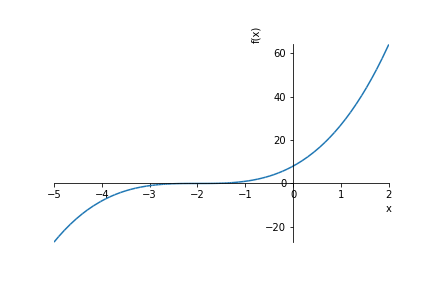
\includegraphics[width=0.75\linewidth]{images/Ch07_SymbolicFigure1} 

}

\caption{A plot of a symbolically defined function.}\label{fig:unnamed-chunk-833}
\end{figure}

\begin{center}\rule{0.5\linewidth}{0.5pt}\end{center}

\begin{example}
\protect\hypertarget{exm:unnamed-chunk-834}{}{\label{exm:unnamed-chunk-834} }Multiple plots can be done at the same time with the \texttt{sympy.plot} command.

Plot \(f(x) = (x+2)^3\) and \(g(x) = 20\cos(x)\) on the same axes on the domain \(x \in [-5,2]\).
\end{example}

\begin{Shaded}
\begin{Highlighting}[]
\ImportTok{import}\NormalTok{ sympy }\ImportTok{as}\NormalTok{ sp}
\NormalTok{x }\OperatorTok{=}\NormalTok{ sp.Symbol(}\StringTok{\textquotesingle{}x\textquotesingle{}}\NormalTok{)}
\NormalTok{f }\OperatorTok{=}\NormalTok{ (x}\OperatorTok{+}\DecValTok{2}\NormalTok{)}\OperatorTok{**}\DecValTok{3}
\NormalTok{g }\OperatorTok{=} \DecValTok{20}\OperatorTok{*}\NormalTok{sp.cos(x)}
\NormalTok{sp.plot(f, g, (x,}\OperatorTok{{-}}\DecValTok{5}\NormalTok{,}\DecValTok{2}\NormalTok{))}
\end{Highlighting}
\end{Shaded}

\begin{figure}

{\centering 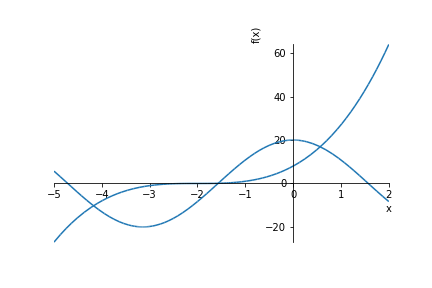
\includegraphics[width=0.75\linewidth]{images/Ch07_SymbolicFigure2} 

}

\caption{A second plot of symbolically defined functions.}\label{fig:unnamed-chunk-836}
\end{figure}

\begin{center}\rule{0.5\linewidth}{0.5pt}\end{center}

\begin{exercise}
\protect\hypertarget{exr:unnamed-chunk-837}{}{\label{exr:unnamed-chunk-837} }Make a symbolic plot of the function \(f(x) = x^3 \ln(x) - 7\) on the domain \([0,3]\).
\end{exercise}

\hypertarget{ch:writing}{%
\chapter{Mathematical Writing}\label{ch:writing}}

This appendix is designed to give you helpful hints for the writing
requires of the homework and the projects. You will find that
mathematical writing is different than writing for literature, for
general consumption, or perhaps other scientific disciplines. Pay
careful attention to the conventions mentioned in this chapter when you
write the results for your projects especially.

A few words of advice:

\begin{itemize}
\item
  Do all of the math first without worrying too much about the
  writing.
\item
  When you have your mathematical results you can start writing.
\item
  Write the introduction last since at that point you know what you've
  written.
\item
  You will spend more time creating well-crafted figures than any
  other part of a mathematical writing project. Expect the figures to
  take at least as long as the math, the writing, and the editing.
\end{itemize}

\hypertarget{the-paper}{%
\section{The Paper}\label{the-paper}}

Write your work in a formal paper that is typed and written at a college
level using appropriate mathematical typesetting. This paper must be
organized into sections, starting with a Summary or Abstract, followed
by an Introduction, and ending with Conclusions and References. Each of
these sections should begin with these headings in a large bold font
(using the LaTeX~\texttt{\textbackslash{}section} and \texttt{\textbackslash{}subsection} commands where
appropriate). Within sections I would suggest using subheadings to
further organize things and aid in clarity.

\hypertarget{figures-and-tables}{%
\section{Figures and Tables}\label{figures-and-tables}}

Figures and tables are a very important part of these projects. Never
break tables or figures across pages. Each figure or table must fit
completely onto one sheet of paper. If your table has too much
information to fit onto one sheet, divide it into two separate tables.
In addition to the figure, this sheet must contain the figure number,
the figure title, and a brief caption; for example ``Figure 2: A plot of
heating oil price versus time from Model F1. We see that the effects of
seasonal variation in price are dominated by random fluctuations.'' In
the text, refer to the figure/table by its number. For example in the
text you might say ``As we see in Figure 2, in model F1 the effects of
seasonal variation in price are dominated by random fluctuations.'' Every
figure and table must be mentioned (by number) somewhere in the text of
your paper. If you do not refer to it anywhere in the text, then you do
not need it, and subsequently it will be ignored.

Think of figures and tables as containing the evidence that you are
using to support the point you are trying to make with your paper.
Always remember that the purpose of a figure or a table is to show a
pattern, and when someone looks at the figure this pattern should be
obvious. Figures should not be cluttered and confusing: They should make
things very clear. Always label the horizontal and vertical axes of
plots.

\hypertarget{writing-style}{%
\section{Writing Style}\label{writing-style}}

The real goal of mathematical writing is to take a complex and intricate
subject and to explain it so simply and so plainly that the results are
obvious for everyone. I want your paper to demonstrate that you not only
did the right calculations, but that you understand what you did and why
your methods worked.

Write this paper using the word `we' instead of `I.' For example: ``First
we calculate the sample mean.'' This `we' refers to you and the reader as
you guide the reader through the work that you've done. Also please
avoid the word ``prove'' or ``proof.'' Numerical methods usually deal with
approximations, not absolutes, and in mathematics we reserve the word
``prove'' for things that are absolutely 100\% certain. Often the word
``test'' can be used instead of ``prove.''

\hypertarget{tips-for-writing-clear-math}{%
\section{Tips For Writing Clear Math}\label{tips-for-writing-clear-math}}

At this point you know just enough mathematics and LaTeX~to be
dangerous. It is time to clean up your act and teach you some of the
formalities about writing mathematics. The following sections stem from
a document that I give all of my upper level mathematics students.

\hypertarget{audience}{%
\subsection{Audience}\label{audience}}

The following suggestions will help you to submit properly written
homework solutions, papers, projects, labs, and proofs. The goal of any
writing is to clearly communicate ideas to another person. Remember that
the other person may even be your future self. When you write for
another person, you will need to include ideas that may be in your mind
but omitted when you are writing a rough draft on scratch paper. If you
keep your intended audience in mind, you will produce higher quality
work. For a course in mathematics, the intended audience is usually your
instructor, your classmates, or a student grader. This implies that your
task is to show that you thoroughly understand your solution.
Consequently, you should routinely include more details.

One rule of thumb must prevail throughout all mathematical writing:

\begin{quote}
When you read a mathematical solution out loud it needs to make sense
as grammatically correct English writing. This includes reading all of
the symbols with the proper language.

\textbf{Don't forget that mathematics is a language that is meant to be
spoken and read just like works of literature!}
\end{quote}

\hypertarget{how-to-make-mathematics-readable-10-things-to-do}{%
\subsection{How To Make Mathematics Readable -- 10 Things To Do}\label{how-to-make-mathematics-readable-10-things-to-do}}

\begin{enumerate}
\def\labelenumi{\arabic{enumi}.}
\item
  When read aloud, the text and formulas must form complete English
  sentences. If you get lost, say aloud what you mean and write it
  down.
\item
  Every mathematical statement must be complete and meaningful. Avoid
  fragments.
\item
  If a statement is something you want to prove or something you
  assume temporarily, e.g., to discuss possible cases or to get a
  contradiction, say so clearly. Otherwise, anything you put down must
  be a true statement that follows from your up front assumptions.
\item
  Write what your plan is. It will also help you focus on what to do.
\item
  There must be sufficient detail to verify your argument. If you do
  not have the details, you have no way of knowing if what you wrote
  is correct or not. Keep the level of detail uniform.
\item
  If you are not sure, even slightly, about something, work out the
  details on the side with utmost honesty, going as deep as necessary.
  Decide later how much detail to include.
\item
  Do not write irrelevant things just to fill paper and show you know
  something.
\item
  Your argument should flow well. Make the reading easy. Logical and
  intuitive notation matters.
\item
  Keep in mind what the problem is and make sure you are not doing
  something else. Many problems are solved and proofs done simply by
  understanding what is what.
\item
  The state of mind when you are inventing a solution is completely
  different from the mode of work when you are writing the solution
  down and verifying it. Learn how to go back and forth between the
  two. The act of typing your solutions forces you to iterate over
  this process but remember that the process isn't done until you've
  proofread what you typed.
\end{enumerate}

\hypertarget{some-writing-tips}{%
\subsection{Some Writing Tips}\label{some-writing-tips}}

\begin{description}
\item[Use sentences:]
The feature that best distinguishes between a properly written
mathematical exposition and a piece of scratch paper is the use (or
lack) of sentences. Properly written mathematics can be read in the
same manner as properly written sentences in any other discipline.
Sentences force a linear presentation of ideas. They provide the
connections between the various mathematical expressions you use.
This linearity will also keep you from handing in a page with
randomly scattered computations with no connections. The sentences
may contain both words and mathematical expressions. Keep in mind
that the way your present your solution may be different than the
way that you arrived at the solution. It is imperative that you work
problems on scratch paper first before formally writing the
solution.

The following extract illustrates these ideas.

\begin{quote}
Let \(n\) be odd. Then Definition 3.10 indicates that there does not
exist an integer, \(k\), such that \(n = 2k\). That is, \(n\) is not
divisible by \(2\). The Quotient-- Remainder theorem asserts that
\(n\) can be uniquely expressed in the form \(n = 2q + r\) , where \(r\)
is an integer with \(0 \le r < 2\). Thus, \(r \in  \{0, 1\}\). Since \(n\) is not divisible by 2, the only
admissible choice is \(r =  1\). Thus, \(n = 2q + 1\), with \(q\) an integer.
\end{quote}
\item[Read out loud:]
The sentences you write should read well out loud. This will help
you to avoid some common mistakes. Avoid sentences like:

\begin{quote}
Suppose the graph has \(n\) number of vertices.\\
The piggy bank contains \(n\) amount of coins.
\end{quote}

If you substitute an actual number for \(n\) (such as 4 or 6) and read
these out loud they will sound wrong (because they are wrong). The
variable \(n\) is already a numeric variable so it should be read just
like an actual number. The correct versions are:

\begin{quote}
Suppose the graph has \(n\) vertices.\\
(Read this as: ``Suppose the graph has en vertices''.)\\
The piggy bank contains \(n\) coins.
\end{quote}

You should also avoid sentences like:

\begin{quote}
From the previous computation \(x=5\) is true.
\end{quote}

A better way to say this is:

\begin{quote}
From the previous computation we see that \(x=5\).
\end{quote}

When you read the equal sign as part of the sentence you realize
that there is no reason to write ``is true''.
\item[\(=\) is NOT a conjunction:]
The mathematical symbol \(=\) is an assertion that the expression on
its left and the expression on its right are equal. Do not use it as
a connection between steps in a series of calculations. Use words
for this purpose. Here is an example that misuses the \(=\) symbol
when solving the equation \(3x=6\):
\[\text{Incorrect! } \qquad 3x = \underbrace{6 =
            \frac{3x}{3}}_{\text{false!}} = \frac{6}{3} = x = 2\]
One proper way to write his is:\\
\(3x=6\). Dividing both sides by \(3\) leads to \(\frac{3x}{3} =  \frac{6}{3}\), which simplifies to \(x=2\).
\item[``\(\implies\)'' means ``implies'':]
The double arrow ``\(\implies\)'' means that the statement on the left
logically implies the statement on the right. This symbol is often
misused in place of the ``\(=\)'' sign.
\item[Do not merge steps:]
Suppose you need to calculate the final price for a \$20 item with
7\% sales tax. One strategy is to first calculate the tax, then add
the \$20. Here is an incorrect way to write this.\\
\[\text{Incorrect! } \qquad  20 \cdot 0.07 \underbrace{=}_{false!} 1.4 +
            20 \underbrace{=}_{false!} \$21.4.\] The main problem
(besides the magically-appearing dollar sign at the end) is that
\(20 \cdot 0.07 \neq 1.4 + 20\). The writer has taken the result of
the multiplication (\(1.4\)) and merged directly into the addition
step, creating a lie (since \(1.4\neq 21.4\)). The calculations could
be written as:
\[\$20 \cdot 0.07 = \$1.40 \text{ so the total price is } \$1.40 + \$20 = \$21.40\]
\item[Avoid ambiguity:]
When in doubt, repeat a noun rather using unspecific words like ``it''
or ``the''. For example, in the sentences

\begin{quote}
Let \(G\) be a simple graph with \(n \ge 2\) vertices that is not
complete and let \(G\) be its complement. Then it must contain at
least one edge.
\end{quote}

there is some ambiguity about whether ``it'' refers to \(G\) or to the
complement of \(G\). The second sentence is better written as ``Then G
must contain at least one edge''.
\item[Use Proper Notation:]
There are many notational conventions in mathematics. You need to
follow the accepted conventions when using notation. For example, A
summation or integral symbol always needs something to act on. The
expressions \[\sum_{i=1}^n \qquad \qquad \int_a^b\] by themselves
are meaningless. The expressions
\[\sum_{i=1}^n a_n \qquad \qquad \int_a^b f(x) dx\] have
well-understood meanings.

An another example,
\[\underbrace{\lim_{h \to 0} = \frac{2x+h}{2}}_{\text{incorrect!}} = \frac{2x}{2} = x\]
is incorrect. It should be written
\[\lim_{h \to 0} \frac{2x+h}{2} = \frac{2x}{2} = x\]
\item[Parenthesis are important:]
Parenthesis show the grouping of terms, and the omission of
parenthesis can lead to much unneeded confusion. For example,
\[x^2 + 5 \cdot x-3 \quad \text{ is very different than } \quad \left( x^2 + 5
            \right) \cdot \left( x-3 \right).\] This is very
important in differentiation and summation notation:
\[\frac{d}{dx} \sin(x) + x^2 \quad \text{is not the same as} \quad \frac{d}{dx}
            \left( \sin(x) + x^2 \right)\]
\[\sum_{k=1}^n 2k+3 \quad \text{is not the same as} \quad \sum_{k=1}^n \left(
            2k+3 \right)\]
\item[Label and reference equations:]
When you need to refer to an equation later it is common practice to
label the equation with a number and then to refer to this equation
by that number. This avoids ambiguity and gives the reader a better
chance at understanding what you're writing. Furthermore, avoid
using words like ``below'' and ``above'' since the reader doesn't really
know where to look. One implication to this style of referencing is
that you should never reference an equation before you define it.\\
\textbf{Incorrect:}

\begin{quote}
In the equation below we consider the domain \(x \in (-1,1)\)
\[f(x) = \sum_{j=1}^\infty \frac{x^n}{n!}.\]
\end{quote}

\textbf{Correct:}

\begin{quote}
Consider the summation \[\begin{aligned}
 f(x) = \sum_{j=1}^\infty \frac{x^n}{n!}.\end{aligned}\]
In this equation we are assuming the domain
\(x \in (-1,1).\)
\end{quote}
\item[``Timesing'':]
The act of multiplication should not be called ``timesing'' as in ``I
can times 3 and 5 to get 15''. The correct version of this sentence
is ``I can multiply 3 and 5 to get 15''. The phrase ``3 times 5 is 15'',
on the other hand, is correct and is likely the root of the
confusion. The mathematical operation being performed is not called
``timesing''. It seems as if this is an unfortunate carry over from
childhood when a child hears ``3 times 5'', sees ``\(3  \times 5\)'', and then incorrectly associates the symbol
``\(\times\)'' with the word multiply in the statement ``I can multiply 3
and 5 to get 15''.
\end{description}

\hypertarget{mathematical-vocabulary}{%
\subsection{Mathematical Vocabulary}\label{mathematical-vocabulary}}

\begin{description}
\item[Function:]
The word function can be used to refer just to the name of a
function, such as ``The function \(s(t)\) gives the position of the
particle as a function of time.'' Or function can refer to both the
function name and the rule that describes the function. For example,
we could elaborate and say, ``The function \(s(t) = t2 - 3t\) gives the
position of the particle as a function of time.'' Notice that both
times the word function is used twice, where the second usage is
describing the mathematical nature of the relationship between time
and position. (Remember that if position can be described as a
function of time, then the position can be uniquely determined from
the time.)
\item[Equation:]
To begin with, an equation must have an equal sign (\(=\)), but just
having an equal sign isn't enough to deserve the name equation.
Generally, an equation is something that will be used to solve for a
particular variable, and/or it expresses a relationship between
variables. So you might say, ``We solved the equation \(x + y = 5\) for
\(x\) to find that \(x = 5 - y\),'' or you might say ``The relationship
between the variables can be expressed with the following equation:
\(xy = 2z\).''
\item[Formula:]
A formula might in fact be an equation or even a function, but
generally the word formula is used when you are going to substitute
numbers for some or all of the variables. For example, we might say,
``The formula for the area of a circle is \(A = \pi r^2\). Since
\(r = 2\) in this case, we find \(A = \pi  2^2 = 4\pi\).'' The bottom line: If you're going to use
algebra to solve for a variable, call it an equation. If you're
going to use it exactly as it is and just put in numbers for the
variables, then call it a formula.
\item[Definition:]
A definition might be any of the above, but it is specifically being
used to define a new term. For example, the definition of the
derivative of a function \(f\) at a point a is
\[f'(a) = \lim_{h \to 0} \frac{f(a+h)-f(a)}{h}.\] Now this does give
us a formula to use to compute the derivative, but we prefer to call
this particular formula a definition to highlight the fact that this
is what we have chosen the word derivative to mean.
\item[Expression:]
The word expression is used when there isn't an equal sign. You
probably won't need this word very often, but it is used like this:
``The factorization of the expression \(x^2 - x - 6\) is
\((x - 3)(x + 2)\).''
\item[Solve/Evaluate:]
Equations are solved, whereas functions are evaluated. So you would
say, ``We solved the equation for \(x\),'' but you would say ``We
evaluated the function at \(x = 5\) and found the function value to be
\(26\).''
\item[Add Subtract vs Plus Minus:]
The word subtract is used when discussing what needs to be done:
``Subtract two from five to get three.'' Add is used similarly: ``Add
two and five to get seven.'' Minus is used when reading a
mathematical equation or expression. For example, the equation
\(x - y = 5\) would be read as ``\(x\) minus \(y\) is equal to five''. Plus
is used similarly. So the equation \(x + y  = 5\) would be read as ``\(x\) plus \(y\) is equal to five''. Some
things we don't say are ``We plus 2 and 5 to get 7'' or ``We minus \(x\)
from both sides of the equation.''
\item[Number/Amount:]
The word number is used when referring to discrete items, such as
``there were a large number of cougars'', or ``there are a large number
of books on my shelf''. The word amount is used when referring to
something that might come in a pile, such as ``that is a huge amount
of sand!'' or, ``I only use a small amount of salt when I cook''.
\item[Many/Much:]
These words are used in much the same way as number and amount, with
many in place of number and much in place of amount. For example, we
might say, ``There aren't as many cougars here as before'', or ``I
don't use as much salt as you do.''
\item[Fewer/Less:]
These are the diminutive analogues of many and much. So, ``There are
fewer cougars here than before'', or ``You use less salt than I do.''
\end{description}

\hypertarget{sensitivity-analysis}{%
\section{Sensitivity Analysis}\label{sensitivity-analysis}}

(This section is paraphrased partly from Dianne O'Leary's book
\emph{Computing in Science \& Engineering} and partly from Mark Meerschaert's
text \emph{Mathematical Modeling}.)

In contrast to to classroom exercises, the real world rarely presents us
with a problem in which the data is known with absolute certainty. Some
parameters (such as \(\pi\)) we can define with certainty, and others
(such as Planck's constant \(\hslash\)) we know to high precision, but
most data is measured and therefore contains measurement error.

Thus, what we really solve isn't the problem we want, but some \emph{nearby}
problem, and in addition to reporting the computed solution we really
need to report a bound on either

\begin{itemize}
\item
  the difference between the true solution and the computed solution,
  or
\item
  the difference between the problem we solved and the problem we
  wanted to solve.
\end{itemize}

This need occurs throughout computational science. For example,

\begin{itemize}
\item
  If we compute the resonant frequencies of a model of a building, we
  want to know how these frequencies change if the load within the
  building changes.
\item
  If we compute the stresses on a bridge, we want to know how
  sensitive these values are to changes that might occur as the bridge
  ages.
\item
  If we develop a model for our data and fit the parameters using
  least squares, we want to know how much the parameters would change
  if the data were wiggled within the uncertainty limits.
\end{itemize}

One of the best ways to measure the sensitivity of a parameter \(k\) on an
output \(x\) is to measure the ratio between the relative change in \(x\) to
the relative change in \(k\). That is, one measure of sensitivity is
\[S = \Big| \left( \frac{\Delta x}{x} \right) \Big/ \left( \frac{\Delta k}{k} \right)
    \Big|.\] Simplifying a bit gives
\[S = \Big| \left( \frac{\Delta x}{\Delta k} \right) \cdot \left( \frac{k}{x(k)} \right)
    \Big|\] where we are now explicitly stating that the output \(x\) is a
function of \(k\): \(x=x(k)\). Taking \(\Delta k = \delta\) as well as taking
\(\Delta x = x(x\pm\delta)-x(k)\) we can rewrite one more time to give
\[S = \Big|\left( \frac{x(k\pm\delta)-x(k)}{\delta} \right) \cdot \left( \frac{k}{x(k)}
    \right) \Big|.\] Notice that we could take the change of \(x\) by
increasing \(k\) by \(\delta\) or by decreasing \(k\) by \(\delta\).

The value of \(\delta\) is related to known or estimated information about
how the parameter varies. It is likely that \(k\) is a value from some
statistical distribution (like a normal distribution) with an
approximately known or estimated standard deviation. The value of
\(\delta\) should be related to the standard deviation and some basic
statistics can be used to choose the \(\delta\) for your sensitivity
analysis. Recall that if you sample a parameter from the normal
distribution then

\begin{itemize}
\item
  roughly 68\% of the sampled parameters will be within 1 standard
  deviation of the mean of the normal distribution, and
\item
  roughly 95\% of the sampled parameters will be within \(1.96\) standard
  deviations of the mean of the normal distribution.
\end{itemize}

This means that if \(k\) comes from a normal distribution then a very
typical choice for \(\delta\) is \(1.96\) times the value of the estimated
standard deviation (up or down from \(k\)). If, on the other hand, the
values of the parameter are uniformly distributed then \(\delta\) can be
chosen as the maximum estimated deviation from the mean of the
distribution (up or down from \(k\)).

Generally:

\begin{itemize}
\item
  If the value of \(S\) is approximately 1 then the relative changes are
  approximately the same and the output is not very sensitive to
  changes in the parameter.
\item
  If the value of \(S\) is less than 1 then the relative changes in the
  output are less than the changes in the parameter and the output is
  not sensitive to changes in the parameter.
\item
  Finally, if the value of \(S\) is larger than 1 then the relative
  changes in the output are greater than the changes in the parameter
  and the output is considered sensitive to changes in the parameter.
\end{itemize}

\hypertarget{example-of-sensitivity-analysis}{%
\subsection{Example of Sensitivity Analysis}\label{example-of-sensitivity-analysis}}

Let's do a more specific example. If we are analyzing the differential
equation \(P' = kP\) and we estimate that the growth rate is normally
distributed with sample mean \(k \approx 0.009\) and a standard deviation of \(\sigma \approx 0.001\), then we can
estimate the sensitivity of the time needed for the population to double
as a function of the growth rate. In this case, the \emph{doubling time} is
the output and the \emph{growth rate} is the parameter of interest.

The analytic solution to the differential equation is
\(P(t) = P_0 e^{kt}\) and the population doubling can be found by solving
\(2P_0 = P_0 e^{kT_d}\) where \(T_d\) is the time to double the population.
Using some basic algebra we see that the doubling time as a function of
the growth rate is \(T_d(k) = \frac{\ln(2)}{k}\). Therefore, to measure
the sensitivity of the doubling time to changes in the parameter \(k\) we
can take \(\delta = 1.96 \times 0.001 = 0.00196\). To measure sensitivity in doubling time
to an increase in the growth rate we see that \(S\) is given as follows:
\[\begin{aligned}
    S &= \Big| \left( \frac{T_d(k+\delta)-T_d(k)}{\delta} \right) \cdot \left(
    \frac{k}{T_d(k)} \right) \Big| \\
    &= \Big| \left(\frac{\frac{\ln(2)}{k+\delta} -
    \frac{\ln(2)}{k}}{\delta}  \right) \cdot \left( \frac{k}{\frac{\ln(2)}{k}} \right)
    \Big| \\
    & = \Big| \left( \frac{k\ln(2) - (k+\delta)\ln(2) }{\delta k(k+\delta)} \right) \cdot \left(
    \frac{k^2}{\ln(2)} \right) \Big|  \\
    &= \Big| \frac{k}{k+\delta} \Big| \\
    &= \frac{0.009}{0.009 + 1.96 \times 0.001} = \frac{0.009}{0.01096} \approx
    0.8212\end{aligned}\] To measure sensitivity in doubling time to a
decrease in the growth rate we see that \(S\) is given as\footnote{I'm showing you the algebra here, but it really isn't necessary to
  show this level of routine algebra in your papers. Only show the
  algebra and other calculations that are necessary for the reader to
  understand the work that you're doing.}
\[\begin{aligned}
    S &= \Big| \left( \frac{T_d(k-\delta)-T_d(k)}{\delta} \right) \cdot \left(
    \frac{k}{T_d(k)} \right) \Big| \\
    &= \Big| \left(\frac{\frac{\ln(2)}{k-\delta} -
    \frac{\ln(2)}{k}}{\delta}  \right) \cdot \left( \frac{k}{\frac{\ln(2)}{k}} \right)
    \Big| \\
    & = \Big| \left( \frac{k\ln(2) - (k-\delta)\ln(2) }{\delta k(k-\delta)} \right) \cdot \left(
    \frac{k^2}{\ln(2)} \right) \Big|  \\
    &= \Big| \frac{k}{k-\delta} \Big| \\
    &\approx \frac{0.009}{0.009 - 1.96 \times 0.001} = \frac{0.009}{0.00704} \approx
    1.2784.\end{aligned}\]

In the present example, the doubling time is not considered to be very
sensitive to increases in the growth rate but it is sensitive to
decreases in the growth rate. Given that in this simple example we are
dealing with an exponential decay function this should also be
intuitively \emph{obvious}.

\hypertarget{ch:extras}{%
\chapter{Optional Material}\label{ch:extras}}

This Appendix contains a few sections that are considered optional for
the course as we teach it. Instructors may be interested
in expanding upon what is here for their classes.

\hypertarget{interpolation}{%
\section{Interpolation}\label{interpolation}}

The least squares problem that we studied in Chapter \ref{ch:linearalgebra} seeks to find a best fitting function that is \emph{closest} (in the Euclidean distance sense) to a set of data. What if, instead, we want to match the data points with a function. This is the realm of interpolation. Take note that there are many many forms of interpolation that are tailored to specific problems. In this brief section we cover only a few of the simplest forms of interpolation involving only polynomial functions. The problem that we'll focus on can be phrased as:\\
\emph{Given a set of \(n+1\) data points \((x_0, y_0), (x_1, y_1), \ldots, (x_n,y_n)\), find a polynomial of degree at most \(n\) that \textbf{exactly} matches these points.}

\hypertarget{vandermonde-interpolation}{%
\subsection{Vandermonde Interpolation}\label{vandermonde-interpolation}}

\begin{exercise}
\protect\hypertarget{exr:unnamed-chunk-838}{}{\label{exr:unnamed-chunk-838} }Consider the data set
\[S = \{ (0,1) \, , \, (1,2) \, , \, (2,5) \, , \, (3,10) \}.\]
If we want to fit a polynomial to this data then we can use a cubic function (which has 4
parameters) to match the data perfectly. Why is a cubic polynomial the best choice?
\end{exercise}

\begin{center}\rule{0.5\linewidth}{0.5pt}\end{center}

\begin{exercise}
\protect\hypertarget{exr:unnamed-chunk-839}{}{\label{exr:unnamed-chunk-839} }Using the data from the previous problem, if we choose \(p(x) = \beta_0 + \beta_1 x + \beta_2 x^2 + \beta_3 x^3\) then the resulting system of equations is
\[\begin{pmatrix}  1 & 0 & 0 & 0 \\
                    1 & 1 & 1 & 1 \\
                    1 & 2 & 4 & 8 \\
                    1 & 3 & 9 & 27 \end{pmatrix} \begin{pmatrix} \beta_0 \\ \beta_1 \\
                    \beta_2 \\ \beta_3 \end{pmatrix} = \begin{pmatrix} 1 \\ 2 \\ 5 \\ 10
            \end{pmatrix}.\]

\begin{enumerate}
\def\labelenumi{\alph{enumi}.}
\tightlist
\item
  Notice that the system of equations is square (same number of equations and unknowns). Why is this important?
\item
  Solve the system for \(\beta_1, \beta_2, \beta_3\) and \(\beta_4\) using any method discussed in Chapter \ref{ch:linearalgebra}.
\item
  Write the final polynomial \(p(x)\) and verify that it matches the data points exactly.\\
\item
  Make a plot showing the data and your interoplated polynomial.
\end{enumerate}
\end{exercise}

\begin{center}\rule{0.5\linewidth}{0.5pt}\end{center}

\begin{definition}[Vandemonde Interpolation]
\protect\hypertarget{def:unnamed-chunk-840}{}{\label{def:unnamed-chunk-840} \iffalse (Vandemonde Interpolation) \fi{} }Let \(S = \{(x_0,y_0) \,,\, (x_1,y_1) \,,\, \ldots, (x_n,y_n)\}\) be a set of ordered pairs where the \(x\) values are all unique. The goal of interpolation is to find a function \(f(x)\) that matches the data exactly. Vandermonde interpolation uses a polynomial of degree \(n-1\) since with such a polynomial we have \(n\) unknowns and we can solve the least squares problem exactly. Doing so, we arrive at the system of equations
\[\begin{aligned}
        \begin{pmatrix} 1 & x_0 & x_0^2 & \cdots & x_0^n \\
                        1 & x_1 & x_1^2 & \cdots & x_1^n \\
                        1 & x_2 & x_2^2 & \cdots & x_2^n \\
                        \vdots & \vdots & \vdots & \ddots & \vdots \\
                        1 & x_n & x_n^2 & \cdots & x_n^n \end{pmatrix}
        \begin{pmatrix} \beta_0 \\ \beta_1 \\ \beta_2 \\ \vdots \\ \beta_n \end{pmatrix}
        =
        \begin{pmatrix} y_0 \\ y_1 \\ y_2 \\ \vdots \\ y_n \end{pmatrix}.
    \end{aligned}\]
The matrix on the left-hand side of is called the \textbf{Vandermonde Matrix}.
\end{definition}

\begin{center}\rule{0.5\linewidth}{0.5pt}\end{center}

\begin{exercise}
\protect\hypertarget{exr:unnamed-chunk-841}{}{\label{exr:unnamed-chunk-841} }Write a python function that accepts an array of ordered pairs (where each \(x\) value is unique) and builds a Vandermonde interpolation polynomial. Test your function on the simple example given above and then on several larger problems. It may be simplest to initially test on data generated from functions that we know.
\end{exercise}

\begin{center}\rule{0.5\linewidth}{0.5pt}\end{center}

\begin{exercise}
\protect\hypertarget{exr:unnamed-chunk-842}{}{\label{exr:unnamed-chunk-842} }Build a Vandermonde interpolation polynomial to interpolate the function \(f(x) = \cos(2 \pi x)\) with \(n\) points that are linearly spaced on the interval \(x \in [0,2]\). Repeat this experiment with \(n=5\), \(n=10\), \(n=15\), \(\ldots\), \(n=100\). Make a plot for each value of \(n\). What do you observe?
\end{exercise}

\begin{center}\rule{0.5\linewidth}{0.5pt}\end{center}

\begin{exercise}
\protect\hypertarget{exr:unnamed-chunk-843}{}{\label{exr:unnamed-chunk-843} }Vandermonde interpolation is relatively easy to conceptualize and code, but there is an inherent problem. Use your Vandemonde interploation code to create a plot where the horizontal axis is the order of the interpolating polynomial
and the vertical axis is the ratio of the maximum eigenvalue to the minimum eigenvalue of the Vandemonde matrix \(|\lambda_{max}|/|\lambda_{min}|\). What does this plot tell you about Vandermonde interpolation for high-order polynomials? You can use the same model function as from the previous exercise.
\end{exercise}

\begin{center}\rule{0.5\linewidth}{0.5pt}\end{center}

\hypertarget{lagrange-interpolation}{%
\subsection{Lagrange Interpolation}\label{lagrange-interpolation}}

Lagrange interpolation is a rather clever interpolation scheme where we build up the interpolating polynomial from simpler polynomials. For interpolation we
want to build a polynomial \(p(x)\) such that \(p(x_j) = y_j\) for every datapoint in the set \(\{(x_1,y_1), (x_2, y_2), \ldots, (x_n,y_n)\}\). If we can find a polynomial \(\phi_j(x)\) such that
\[\phi_j(x) = \left\{ \begin{array}{ll} 0, & \text{ if } x = x_i \text{ and } i \ne j \\ 1, & \text{ if
    } x=x_j \end{array} \right.\]
then for Lagrange interpolation we build \(p(x)\) as a linear combination of the \(\phi_j\) functions. Let's look at an example.

\begin{center}\rule{0.5\linewidth}{0.5pt}\end{center}

\begin{exercise}
\protect\hypertarget{exr:unnamed-chunk-844}{}{\label{exr:unnamed-chunk-844} }Consider the data set
\(S = \{(0,1) \, , \, (1,2) \, , \, (2,5) \, , \, (3,10) \}\).

\begin{enumerate}
\def\labelenumi{\alph{enumi}.}
\item
  Based on the descriptions of the \(p(x)\) and \(\phi_j(x)\) functions,
  why would \(p(x)\) be defined as
  \[p(x) = 1 \phi_0(x) + 2 \phi_1(x) + 5 \phi_2(x) + 10 \phi_3(x)?\]
\item
  Verify that \(\phi_0(x)\) can be defined as
  \[\phi_0(x) = \frac{(x-1)(x-2)(x-3)}{(0-1)(0-2)(0-3)}.\]
  That is to say, verify that \(\phi_0(0) = 1\) and \(\phi_0(1) = \phi_0(2) = \phi_0(3) = 0\).
\item
  Verify that \(\phi_1(x)\) can be defined as
  \[\phi_1(x) = \frac{(x-0)(x-2)(x-3)}{(1-0)(1-2)(1-3)}.\]
  That is to say, verify that \(\phi_1(1) = 1\) and \(\phi_1(0) = \phi_1(2) = \phi_1(3) = 0\).
\item
  Define \(\phi_2(x)\) and \(\phi_3(x)\) in a similar way.
\item
  Build the linear combination from part (a) and create a plot showing
  that this polynomial indeed interpolates the points in the set \(S\).
\end{enumerate}
\end{exercise}

\begin{center}\rule{0.5\linewidth}{0.5pt}\end{center}

\begin{exercise}
\protect\hypertarget{exr:unnamed-chunk-845}{}{\label{exr:unnamed-chunk-845} }Is the Lagrange interpolation polynomial built form the previous problem the same as the Vandermonde interpolation polynomial for the same data?
\end{exercise}

\begin{center}\rule{0.5\linewidth}{0.5pt}\end{center}

\begin{definition}[Lagrange Interpolation]
\protect\hypertarget{def:unnamed-chunk-846}{}{\label{def:unnamed-chunk-846} \iffalse (Lagrange Interpolation) \fi{} }To build an \textbf{Lagrange polynomial} \(p(x)\) for the set of points
\(\{(x_0,y_0)\,,\,(x_1,y_1)\,,\,(x_2,y_2)\,,\ldots,\,(x_n,y_n)\}\) we
first build the polynomials \(\phi_j(x)\) for each
\(j = 0, 1, 2, \ldots, n\) and then construct the polynomial \(p(x)\) as
\[p(x) = \sum_{j=0}^n y_j \phi_j(x).\] The \(\phi_j(x)\) functions are
defined as \[\phi_j(x) = \prod_{i \ne j} \frac{x-x_i}{x_j-x_i}.\]
\end{definition}

\begin{center}\rule{0.5\linewidth}{0.5pt}\end{center}

\begin{example}
\protect\hypertarget{exm:unnamed-chunk-847}{}{\label{exm:unnamed-chunk-847} }Build a Lagrange interpolation polynomial for the set of points
\[S  = \{(1,5)\,,\,(2,9)\,,\,(3,11)\}.\]

\textbf{Solution:} We first build the three \(\phi_j\) functions.
\[\begin{aligned}
        \phi_0(x) = \frac{(x-2)(x-3)}{(1-2)(1-3)} \\
        \phi_1(x) = \frac{(x-1)(x-3)}{(2-1)(2-3)} \\
        \phi_2(x) = \frac{(x-1)(x-2)}{(3-1)(3-2)}.
    \end{aligned}\]
Take careful note that the \(\phi\) functions are built in a very particular way. Indeed, \(\phi_0(1) = 1\), \(\phi_0(2) =0\), and \(\phi_0(3) = 0\). Also, \(\phi_1(1) = 0\), \(\phi_1(2) = 1)\), and \(\phi_1(3) = 0\). Finally, note that \(\phi_2(1) = 0\), \(\phi_2(1) = 0\) and \(\phi_2(3) = 1\). Thus, the polynomial \(p(x)\) can be built as
\[p(x) = 5 \phi_0(x) + 9 \phi_1(x) + 11 \phi(2(x) = 5 \frac{(x-2)(x-3)}{(1-2)(1-3)} +
    \frac{(x-1)(x-3)}{(2-1)(2-3)} + \frac{(x-1)(x-2)}{(3-1)(3-2)}.\]
The remainder of the simplification is left to the reader.
\end{example}

\begin{center}\rule{0.5\linewidth}{0.5pt}\end{center}

\begin{exercise}
\protect\hypertarget{exr:unnamed-chunk-848}{}{\label{exr:unnamed-chunk-848} }Write a python function that accepts a list of list of ordered pairs (where each \(x\) value is unique) and builds a Lagrange interpolation polynomial. Test your function on several examples.
\end{exercise}

\begin{center}\rule{0.5\linewidth}{0.5pt}\end{center}

\hypertarget{chebyshev-points}{%
\subsection{Chebyshev Points}\label{chebyshev-points}}

\begin{exercise}
\protect\hypertarget{exr:unnamed-chunk-849}{}{\label{exr:unnamed-chunk-849} }Using either Vandermonde or Lagrange interpolation build a polynomial
that interpolates the function \[f(x) = \frac{1}{1+x^2}\] for
\(x \in [-5,5]\) with polynomials of order \(n=2, 3, \ldots\) and linearly
spaced interpolation points. What do you notice about the quality of the
interpolating polynomial near the endpoints?
\end{exercise}

\begin{center}\rule{0.5\linewidth}{0.5pt}\end{center}

\begin{exercise}
\protect\hypertarget{exr:unnamed-chunk-850}{}{\label{exr:unnamed-chunk-850} }As you should have noticed the quality of the interpolation gets rather
terrible near the endpoints when you use linearly spaced points for the
interpolation. A fix to this was first proposed by the Russian
mathematician Pafnuty Chebyshev (1821-1894). The idea is as follows:

\begin{itemize}
\item
  Draw a semicircle above the closed interval on which you are
  interpolating.
\item
  Pick \(n\) equally spaced points along the semicircle (i.e.~same arc
  length between each point).
\item
  Project the points on the semicircle down to the interval. Use these
  projected points for the interpolation.
\end{itemize}

\begin{enumerate}
\def\labelenumi{\alph{enumi}.}
\tightlist
\item
  Draw a picture of what we just described.
\item
  What do you notice about the \(x\)-values of these projected points? Why might it be desirable to use a collection of points like this for interpolation?
\end{enumerate}
\end{exercise}

\begin{center}\rule{0.5\linewidth}{0.5pt}\end{center}

\begin{definition}[Chebyshev Interpolation Points]
\protect\hypertarget{def:unnamed-chunk-851}{}{\label{def:unnamed-chunk-851} \iffalse (Chebyshev Interpolation Points) \fi{} }It should be clear that since we are projecting down to the \(x\)-axis from a circle then all we need are the cosine values from the circle. Hence we can form the Chebyshev interpolation points for the interval \(x \in [-1,1]\) from the formula
\[\begin{aligned}
    x_j = \cos\left( \frac{\pi j}{n} \right), \quad \text{for} \quad j=0, 1, \ldots, n
    \label{eqn:chebyshev_cosine}\end{aligned}.\]

To transform the Chebyshev points from the interval \([-1,1]\) to the interval \([a,b]\) we can apply a linear transformation which maps \(-1\) to \(a\) and \(1\) to \(b\):
\[x_j \gets \left( \frac{b-a}{2} \right)\left( x_j + 1 \right) + a\]
where the ``\(x_j\)'' on the left is on the interval \([a,b]\) and the ``\(x_j\)''
on the right is on the interval \([-1,1]\).
\end{definition}

\begin{center}\rule{0.5\linewidth}{0.5pt}\end{center}

\begin{exercise}
\protect\hypertarget{exr:unnamed-chunk-852}{}{\label{exr:unnamed-chunk-852} }Consider the function \(f(x) = \frac{1}{1+x^2}\) just as we did for the first problem in this subsection. Write code that overlays an interpolation with linearly spaced points and interpolation with Chebyshev points. Give plots for polynomial of order \(n=2,3, 4, \ldots\). Be sure to show the original function on your plots as well. What do you notice?
\end{exercise}

\begin{center}\rule{0.5\linewidth}{0.5pt}\end{center}

\begin{exercise}
\protect\hypertarget{exr:unnamed-chunk-853}{}{\label{exr:unnamed-chunk-853} }Demonstrate that the Chebyshev interpolation nodes will improve the stability of the Vandermonde matrix over using linearly spaced nodes.
\end{exercise}

\begin{center}\rule{0.5\linewidth}{0.5pt}\end{center}

\hypertarget{sec:mv_newton}{%
\section{Multi-Dimensional Newton's Method}\label{sec:mv_newton}}

Now that we know some linear algebra let's return to the Newton's Method root finding technique from earlier in the book. This time we will consider root finding problems where we are not just solving the equation \(f(x) = 0\) as we did Chapter \ref{ch:algebra}. Instead consider the function \(F\) that takes a vector of variables in and outputs a vector. An example of such a function is
\[F(x,y) = \begin{pmatrix} x\sin(y) \\ \cos(x) + \sin(y^2)
\end{pmatrix}.\]
It should be clear that making a picture of this type of function is a frivolous endeavor! In the case of the previous example, there are two inputs and two outputs so the ``picture'' would have to be four dimensional. Even so, we can still ask the question:\\
\emph{For what values of \(x\) and \(y\) does the function \(F\) give the zero vector?}

That is, what if we have \(F\) defined as
\[F(x,y) = \begin{pmatrix} f(x,y) \\ g(x,y) \end{pmatrix}\]
and want to solve the system of equations
\[\begin{aligned}
    f(x,y) &= 0 \\ 
    g(x,y) &= 0. \end{aligned}\]
In the present problem this amounts to solving the nonlinear system of equations
\[\begin{aligned}
    x\sin(y) &= 0 \\
    \cos(x) + \sin(y^2) &=0.\end{aligned}\]
In this case it should be clear that we are implicitly defining \(f(x,y) = x\sin(y)\) and \(g(x,y) = \cos(x) + \sin(y^2)\). A moment's reflection (or perhaps some deep meditation) should reveal that \((\pm\pi/2,0)\) are two solutions to the system, and given the trig functions it stands to reason that \((\pi/2 + \pi k,\pi j)\) will be a solution for all integer values of \(k\) and \(j\).

\begin{center}\rule{0.5\linewidth}{0.5pt}\end{center}

\begin{exercise}
\protect\hypertarget{exr:unnamed-chunk-854}{}{\label{exr:unnamed-chunk-854} }To build a numerical solver for a nonlinear system of equations, let's just recall Newton's Method in one dimension and then mimic that for systems of higher dimensions. We'll stick to two dimensions in this problem for relative simplicity.

\begin{enumerate}
\def\labelenumi{\alph{enumi}.}
\item
  In Newton's Method we first found the derivative of our function. In
  a nonlinear system such as this one, talking about ``the'' derivative
  is a bit nonsense since there are many first derivatives. Instead we
  will define the Jacobian matrix \(J(x,y)\) as a matrix of the first
  partial derivatives of the functions \(f\) and \(g\).
  \[J(x,y) = \begin{pmatrix} f_x & f_y \\ g_x & g_y \end{pmatrix}.\]
  In the present example (fill in the rest of the blanks),
  \[J(x,y) = \begin{pmatrix} \sin(y) &
                  \underline{\hspace{0.5in}} \\  \underline{\hspace{0.5in}} &
              \underline{\hspace{0.5in}} \end{pmatrix}.\]
\item
  Now let's do some Calculus and algebra. Your job in this part of
  this problem is to follow all of the algebraic steps.

  \begin{enumerate}
  \def\labelenumii{\roman{enumii}.}
  \item
    In one-dimensional Newton's Method we then write the equation of
    a tangent line at a point \((x_0, f(x_0))\) as
    \[f(x) - f(x_0) \approx f'(x_0)(x-x_0)\] to give a local
    approximation to the function. We'll do the exact same thing
    here, but in place of ``\(x\)'' we need to have a vector and in
    place of the derivative we need to have the Jacobian
    \[F(x,y) - F(x_0,y_0) \approx J(x_0, y_0) \left( \begin{pmatrix} x \\ y
            \end{pmatrix} - \begin{pmatrix} x_0 \\ y_0 \end{pmatrix} \right).\]
  \item
    In one-dimensional Newton's Method we then set \(f(x)\) to zero
    since we were ultimately trying to solve the equation
    \(f(x) = 0\). Hence we got the equation
    \[0 - f(x_0) \approx f'(x_0)(x-x_0)\] and then rearranged to
    solve for \(x\). This gave us
    \[x \approx x_0 - \frac{f(x_0)}{f'(x_0)}.\] In the
    multi-dimensional case we have the same goal. If we set \(F(x,y)\)
    to the zero vector and solve for the vector
    \(\begin{pmatrix}x\\y\end{pmatrix}\) then we get
    \[\begin{pmatrix} x\\y\end{pmatrix} \approx \begin{pmatrix}
                   x_0 \\ y_0 \end{pmatrix} -
               \left[ J(x_0,y_0) \right]^{-1} F(x_0,y_0).\] Take
    very careful note here that we didn't divide by the Jacobian. Why not?
  \item
    The final step in one-dimensional Newton's Method was to turn
    the approximation of \(x\) into an iterative process by replacing
    \(x\) with \(x_{n+1}\) and replacing \(x_0\) with \(x_{n}\) resulting in
    the iterative form of Newton's Method
    \[x_{n+1} = x_{n} - \frac{f(x_n)}{f'(x_n)}.\] We can do the
    exact same thing in the two-dimensional version of Newton's
    Method to arrive at
    \[\begin{pmatrix} x_{n+1} \\ y_{n+1} \end{pmatrix} = \begin{pmatrix}
              x_n \\ y_n \end{pmatrix} - J^{-1}(x_n,y_n) F(x_n, y_n).\]
    Writing this in full matrix-vector form we get
    \[\begin{pmatrix} x_{n+1} \\ y_{n+1} \end{pmatrix} = \begin{pmatrix}
                  x_n \\ y_n \end{pmatrix} - \begin{pmatrix} f_x & f_y \\ g_x & g_y
          \end{pmatrix}^{-1} \begin{pmatrix} f(x_n,y_n) \\ g(x_n,y_n) \end{pmatrix}.\]
  \end{enumerate}
\item
  Write down the Newton iteration formula for the system
  \[\begin{aligned}
          x\sin(y) &= 0 \\
          \cos(x) + \sin(y^2) &= 0.
      \end{aligned}\] Do not actually compute the matrix inverse of
  the Jacobian.
\item
  The inverse of the Jacobian needs to be dealt with carefully. We
  typically don't calculate inverses directly in numerical analysis,
  but since we have some other tools to do the work we can think of it
  as follows:

  \begin{itemize}
  \item
    We need the vector \(\boldsymbol{b} = J^{-1}(x_n,y_n) F(x_n,y_n)\).
  \item
    The vector \(\boldsymbol{b}\) is the same as the solution to the equation
    \(J(x_n,y_n) \boldsymbol{b}  = F(x_n,y_n)\) at each iteration of Newton's Method.
  \item
    Therefore we can so a relatively fast linear solve (using any
    technique from Chapter \ref{ch:linearalgebra}) to find \(\boldsymbol{b}\).
  \item
    The Newton iteration becomes
    \[\begin{pmatrix} x_{n+1} \\ y_{n+1} \end{pmatrix} = \begin{pmatrix} x_n \\
                    y_n \end{pmatrix} - \boldsymbol{b}.\]
  \end{itemize}
\end{enumerate}
\end{exercise}

\begin{center}\rule{0.5\linewidth}{0.5pt}\end{center}

\begin{exercise}
\protect\hypertarget{exr:unnamed-chunk-855}{}{\label{exr:unnamed-chunk-855} }Write code to solve the present nonlinear system of equations.
Implement some sort of linear solver within your code and be able to
defend your technique. Try to pick a starting point so that you
find the solution \((\pi/2,\pi)\) on your first attempt at solving
this problem. Then play with the starting point to verify that you
can get the other solutions.
\end{exercise}

\begin{center}\rule{0.5\linewidth}{0.5pt}\end{center}

\begin{exercise}
\protect\hypertarget{exr:unnamed-chunk-856}{}{\label{exr:unnamed-chunk-856} }Test your code from the previous problem on the system of nonlinear
equations \[\begin{aligned}
        1+x^2 - y^2 + e^x\cos(y) &= 0 \\
        2xy + e^x\sin(y) &=0.
    \end{aligned}\] Note here that \(f(x,y) = 1+x^2 - y^2 + e^x\cos(y)\)
and \(g(x,y) = 2xy + e^x \sin(y)\).
\end{exercise}

\begin{center}\rule{0.5\linewidth}{0.5pt}\end{center}

Let's
generalize the process a bit so we can numerically approximate solutions
to systems of nonlinear algebraic equations in any number of dimensions.
The Newton's method that we derived in Chapter \ref{ch:algebra} is only applicable to functions
\(f: \mathbb{R} \to \mathbb{R}\) (functions mapping a real number to a
real number). In the previous problem we build a method for solving the
equation \(F(x,y) = (0,0)\) where \(F: \mathbb{R}^2 \to \mathbb{R}^2\). What
about vector-valued functions in \(n\) dimensions? In particular, we would
like to have an analogous method for finding roots of a function \(F\)
where \(F: \mathbb{R}^k \to \mathbb{R}^k\) for any dimension \(k\).

Let \(\boldsymbol{x}\) be a vector in \(\mathbb{R}^k\), let
\[F(\boldsymbol{x}) = \begin{pmatrix} f_1(\boldsymbol{x}) \\ f_2(\boldsymbol{x}) \\ \vdots \\ f_k(\boldsymbol{x}) \end{pmatrix}\]
be a vector valued function, and let \(J\) be the Jacobian matrix
\[J(\boldsymbol{x}) = 
        \begin{pmatrix} \partial f_1 / \partial x_1(\boldsymbol{x}) & \partial f_1 / \partial
            x_2(\boldsymbol{x}) & \cdots
            & \partial f_1 / \partial x_k(\boldsymbol{x}) \\ 
         \partial f_2 / \partial x_1(\boldsymbol{x}) & \partial f_2 / \partial x_2(\boldsymbol{x}) & \cdots &
         \partial f_2 / \partial x_k(\boldsymbol{x}) \\ 
         \vdots & \vdots & \ddots & \vdots \\
         \partial f_k / \partial x_1(\boldsymbol{x}) & \partial f_k / \partial x_2(\boldsymbol{x}) & \cdots & \partial f_k /
     \partial x_k(\boldsymbol{x}) \end{pmatrix}\] By analogy, the multi-dimensional
Newton's method is \[\boldsymbol{x}_{n+1} = \boldsymbol{x}_n -  J^{-1}(\boldsymbol{x}_n)F(\boldsymbol{x}_n)\] where
\(J^{-1}(\boldsymbol{x}_n)\) is the inverse of the Jacobian matrix evaluated at the
point \(\boldsymbol{x}_n\). Take note that you should not be calculating the inverse directly, but instead you should be using a linear solve to get the vector \(\boldsymbol{b}\) where \(J(\boldsymbol{x}_n) \boldsymbol{b} = F(\boldsymbol{x}_n)\).

\begin{center}\rule{0.5\linewidth}{0.5pt}\end{center}

\begin{exercise}
\protect\hypertarget{exr:unnamed-chunk-857}{}{\label{exr:unnamed-chunk-857} }Write code that accepts any number of functions and an initial vector guess and returns an approximation to the root for the problem \(F(\boldsymbol{x}) = \boldsymbol{0}\).
\end{exercise}

\begin{center}\rule{0.5\linewidth}{0.5pt}\end{center}

\begin{exercise}
\protect\hypertarget{exr:unnamed-chunk-858}{}{\label{exr:unnamed-chunk-858} }Use Newton's method to find an approximate solution to the system of equations
\[\begin{aligned}
    x^2 + y^2 + z^2 &= 100 \\
    xyz &= 1 \\
    x - y - \sin(z) &= 0
\end{aligned}\]
\end{exercise}

\begin{center}\rule{0.5\linewidth}{0.5pt}\end{center}

\begin{exercise}
\protect\hypertarget{exr:unnamed-chunk-859}{}{\label{exr:unnamed-chunk-859} }When will the multi-dimensional version of Newton's Method fail? Compare and contrast this with what you found about the one-dimensional version of Newton's Method in Chapter \ref{ch:algebra}. Extend your discussion to talk about the eigenvalues of the Jacobian matrix for a nonlinear system.
\end{exercise}

\begin{center}\rule{0.5\linewidth}{0.5pt}\end{center}

\begin{exercise}
\protect\hypertarget{exr:unnamed-chunk-860}{}{\label{exr:unnamed-chunk-860} }One place that solving nonlinear systems arises naturally is when we
need to find equilibrium points for systems of differential equations.
Remember that to find the equilibrium points for a first order
differential equation we set the derivative term to zero and solve the
resulting equation.

Find the equilibrium point(s) for the system of differential equations
\[\begin{aligned}
        x' &= \alpha x - \beta xy \\
        y' &= \delta y + \gamma xy
    \end{aligned}\] where \(\alpha = 1, \beta = 0.05, \gamma = 0.01\) and
\(\delta =1\).
\end{exercise}

\begin{center}\rule{0.5\linewidth}{0.5pt}\end{center}

\begin{exercise}
\protect\hypertarget{exr:unnamed-chunk-861}{}{\label{exr:unnamed-chunk-861} }Find the equilibrium point(s) for the system of differential equations
\[\begin{aligned}
        x' &= -0.1 xy - x \\
        y' &= -x + 0.9y \\
        z' &= \cos(y) - xz
    \end{aligned}\] if they exist.
\end{exercise}

\begin{center}\rule{0.5\linewidth}{0.5pt}\end{center}

\begin{exercise}
\protect\hypertarget{exr:unnamed-chunk-862}{}{\label{exr:unnamed-chunk-862} }(This problem is modified from {[}\protect\hyperlink{ref-meerschaert}{6}{]})\\
A manufacturer of lawn furniture makes two types of lawn chairs, one
with a wood frame and one with a tubular aluminum frame. The wood-frame
model costs \$18 per unit to manufacture, and the aluminum-frame model
costs \$10 per unit. The company operates in a market where the number
of units that can be sold depends on the price. It is estimated that in
order to sell \(x\) units per day of the wood-frame model and \(y\) units
per day of the aluminum-frame model, the selling price cannot exceed
\[10 + \frac{31}{\sqrt{x}} + \frac{1.3}{y^{0.2}} \text{ dollars per unit}\]
for wood-frame chairs, and
\[5 + \frac{15}{y^{0.4}} + \frac{0.8}{x^{0.08}} \text{ dollars per unit}\]
for the aluminum chairs. We want to find the optimal production levels.
Write this situation as a multi-variable mathematical model, use a
computer algebra system (or by-hand computation) to find the gradient
vector, and then use the multi-variable Newton's method to find the
critical points. Classify the critical points as either local maximums
or local minimums.
\end{exercise}

\begin{center}\rule{0.5\linewidth}{0.5pt}\end{center}

\hypertarget{refs}{}
\begin{cslreferences}
\leavevmode\hypertarget{ref-R-bookdown}{}%
{[}1{]} Y. Xie, ``Bookdown: Authoring books and technical documents with r markdown.'' \url{https://bookdown.org/yihui/bookdown/}, 2019.

\leavevmode\hypertarget{ref-active-calculus}{}%
{[}2{]} M. Boelkins, ``Active calculus.'' \url{https://activecalculus.org/single/frontmatter.html}, 2018.

\leavevmode\hypertarget{ref-euler}{}%
{[}3{]} ``ProjectEuler.net.'' \url{https://projecteuler.net/}.

\leavevmode\hypertarget{ref-chartier}{}%
{[}4{]} A. Greenbaum and T. Chartier, \emph{Numerical methods: Design, analysis, and computer implementation of algorithms}. Princeton University Press, 2012.

\leavevmode\hypertarget{ref-burden}{}%
{[}5{]} R. Burden, D. Faires, and A. Burden, \emph{Numerical analysis, 10ed}. Cengage Learning, 2016.

\leavevmode\hypertarget{ref-meerschaert}{}%
{[}6{]} M. Meerschaert, \emph{Mathematical modeling, 4ed}. Academic Press, 2013.

\leavevmode\hypertarget{ref-tea}{}%
{[}7{]} E. Sullivan, J. Bauer, and E. Wiens, ``1-094-s-steepingtea.'' Sep. 2017, {[}Online{]}. Available: \url{https://www.simiode.org/resources/4190}.

\leavevmode\hypertarget{ref-plague}{}%
{[}8{]} B. Winkel, ``6-004-s-villageepidemic.'' Jul. 2016, {[}Online{]}. Available: \url{https://simiode.org/resources/2372}.

\leavevmode\hypertarget{ref-bedridden}{}%
{[}9{]} S. Miller, ``6-001-s-epidemic.'' Jun. 2015, {[}Online{]}. Available: \url{https://simiode.org/resources/572}.

\leavevmode\hypertarget{ref-drone}{}%
{[}10{]} R. Spindler, ``6-023-s-droneheadinghome.'' Apr. 2017, {[}Online{]}. Available: \url{https://www.simiode.org/resources/3476}.

\leavevmode\hypertarget{ref-simiodeheat}{}%
{[}11{]} K. Spayd and J. Puckett, ``9-020-t-heatdiffusion.'' Oct. 2019, {[}Online{]}. Available: \url{https://simiode.org/resources/6452}.
\end{cslreferences}

\end{document}
